\documentclass[12pt, a4paper]{article}

% Avoid useless warnings about included images
% Reference: https://tex.stackexchange.com/a/78020
%\pdfsuppresswarningpagegroup=1

% Use \hypersetup here to get rid of the ugly boxes around links
\usepackage{hyperref}
\hypersetup{
  colorlinks=true,
  linkcolor=blue,
  urlcolor=blue
}

% Avoid warning about missing font for \textbackslash character.
\usepackage[T1]{fontenc}

% For nicer paragraph spacing
\usepackage{parskip}

\usepackage[disable]{todonotes}
%\usepackage{todonotes}

\usepackage{amsmath}%
\usepackage{amsfonts}%
\usepackage{amssymb}%
\usepackage{graphicx}
%\usepackage[miktex]{gnuplottex}
%\ShellEscapetrue
\usepackage{epstopdf}
\usepackage{longtable}
\usepackage{floatrow}
\usepackage{makecell}

% Use \setminted here to get horizontal line above and below listings
\usepackage{minted}
\setminted{
   frame=lines,
   framesep=2mm
}

\usepackage{textcomp}
\usepackage{color,soul}
\usepackage[font={small,it}]{caption}
\floatsetup[listing]{style=Plaintop}    
\floatsetup[longlisting]{style=Plaintop}    

% Turn off indentation but allow \indent command to still work.
\newlength\tindent
\setlength{\tindent}{\parindent}
\setlength{\parindent}{0pt}
\renewcommand{\indent}{\hspace*{\tindent}}

\addtolength{\textwidth}{0.8in}
\addtolength{\oddsidemargin}{-.4in}
\addtolength{\evensidemargin}{-.4in}
\addtolength{\textheight}{1.6in}
\addtolength{\topmargin}{-.8in}

\usepackage{longtable,supertabular}
\usepackage{listings}
\lstset{
  frame=top,frame=bottom,
  basicstyle=\ttfamily,
  language=XML,
  tabsize=2,
  belowskip=2\medskipamount
}

% All listings have a left aligned caption. This looks better as the listings themselves are left aligned.
\captionsetup[listing]{justification=justified,singlelinecheck=false}

\usepackage{tabu}
\tabulinesep=1.0mm
\restylefloat{table}

\usepackage{siunitx}
\usepackage{tablefootnote}
\usepackage{multirow}
\usepackage{colortbl}
\usepackage{footmisc}
\newenvironment{longlisting}{\captionsetup{type=listing}}{}
%\usepackage[colorlinks=true]{hyperref}

% Inline code fragments can run over the page boundary without ragged right.
\AtBeginDocument{\raggedright}

\newcommand{\UserGuide}{}

\renewcommand\P{\ensuremath{\mathbb{P}}}
\newcommand\E{\ensuremath{\mathbb{E}}}
\newcommand\Q{\ensuremath{\mathbb{Q}}}
\newcommand\I{\mathds{1}}
\newcommand\F{\ensuremath{\mathcal F}}
\newcommand\V{\ensuremath{\mathbb{V}}}
\newcommand\YOY{{\rm YOY}}
\newcommand\Prob{\ensuremath{\mathbb{P}}}
\newcommand{\D}[1]{\mbox{d}#1}
\newcommand{\NPV}{\mathit{NPV}}
\newcommand{\CVA}{\mathit{CVA}}
\newcommand{\DVA}{\mathit{DVA}}
\newcommand{\FVA}{\mathit{FVA}}
\newcommand{\COLVA}{\mathit{COLVA}}
\newcommand{\FCA}{\mathit{FCA}}
\newcommand{\FBA}{\mathit{FBA}}
\newcommand{\KVA}{\mathit{KVA}}
\newcommand{\MVA}{\mathit{MVA}}
\newcommand{\PFE}{\mathit{PFE}}
\newcommand{\EE}{\mathit{EE}}
\newcommand{\EPE}{\mathit{EPE}}
\newcommand{\ENE}{\mathit{ENE}}
\newcommand{\EEPE}{\mathit{EEPE}}
\newcommand{\EEE}{\mathit{EEE}}
\newcommand{\EAD}{\mathit{EAD}}
\newcommand{\PE}{\mathit{PE}}
\newcommand{\NE}{\mathit{NE}}
\newcommand{\RC}{\mathit{RC}}
\newcommand{\RW}{\mathit{RW}}
\newcommand{\NS}{\mathit{NS}}
\newcommand{\PD}{\mathit{PD}}
\newcommand{\LGD}{\mathit{LGD}}
\newcommand{\DIM}{\mathit{DIM}}
\newcommand{\DF}{\mathit{DF}}
\newcommand{\MA}{\mathit{MA}}
\newcommand{\SCVA}{\mathit{SCVA}}
\newcommand{\bs}{\textbackslash}
\newcommand{\REDY}{\color{red}Y}

\begin{document}

%\title{Open Source Risk Engine \\ User Guide  }
\title{ORE User Guide}
%\author{Quaternion Risk Management Ltd.}
%\author{Acadia Inc.}
\date{16 October 2023}
\maketitle

\newpage

%-------------------------------------------------------------------------------
\section*{Document History}

\begin{center}
\begin{supertabular}{|l|l|p{9cm}|}
\hline
Date & Author & Comment \\
\hline
7 October 2016 & Quaternion & initial release\\
28 April 2017 & Quaternion  & updates for release 2\\
7 December 2017 & Quaternion & updates for release 3\\
20 March 2019 & Quaternion & updates for release 4\\
19 June 2020 & Quaternion & updates for release 5\\
30 June 2021 & Acadia & updates for release 6\\
16 September 2022 & Acadia & updates for release 7\\
6 December 2022 & Acadia & updates for release 8\\
31 March 2023 & Acadia & updates for release 9\\
16 June 2023 & Acadia & updates for release 10\\
16 October 2023 & Acadia & updates for release 11\\
\hline
\end{supertabular}
\end{center}

\newpage

\tableofcontents
\newpage

\section{Introduction}

The {\em Open Source Risk Project} \cite{ORE} aims at providing a transparent platform for pricing and risk analysis
that serves as
%\medskip
\begin{itemize}
\item a benchmarking, validation, training, and teaching reference,
\item an extensible foundation for tailored risk solutions.
\end{itemize}

Its main software project is {\em Open Source Risk Engine} (ORE), an application that provides
\begin{itemize}
\item a Monte Carlo simulation framework for contemporary risk analytics and value adjustments
\item simple interfaces for trade data, market data and system configuration
\item simple launchers and result visualisation in Jupyter, Excel, LibreOffice
\item unit tests and various examples.  
\end{itemize}
ORE is open source software, provided under the Modified BSD License. It is based 
on QuantLib, the open source library for quantitative finance \cite{QL}.

%\medskip
\subsubsection*{Audience}
The project aims at reaching quantitative risk ma\-nage\-ment practitioners (be it in financial institutions, audit
firms, consulting companies or regulatory bodies) who are looking for accessible software solutions, and quant
developers in charge of the implementation of pricing and risk methods similar to those in ORE. Moreover, the project
aims at reaching academics and students who would like to teach or learn quantitative risk management using a freely
available, contemporary risk application.

\subsubsection*{Contributions}
Quaternion Risk Management \cite{QRM} has been committed to sponsoring the Open Source Risk project through ongoing project
administration, through providing an initial release and a series of subsequent releases in order to achieve a wide
analytics, product and risk factor class coverage. Since Quaternion's acquisition by Acadia Inc. in February 2021, Acadia \cite{acadia} is committed to continue the sponsorship. The Open Source Risk project works will continue with former Quaternion now operating as Acadia's Quantitative Services unit. 

The community is invited to contribute to ORE, for example through
feedback, discussions and suggested enhancement in the forum on the ORE site \cite{ORE}, as well as contributions of ORE
enhancements in the form of source code. See the FAQ section on the ORE site \cite{ORE} on how to get involved.

\subsection{Scope}

ORE currently provides portfolio pricing, cash flow generation, market risk analysis and a range of contemporary derivative portfolio analytics. The latter are based on a Monte Carlo simulation framework which yields 
the evolution of various exposure measures:
\begin{itemize}
\item EE aka EPE (Expected Exposure or Expected Positive Exposure)
\item ENE (Expected Negative Exposure, i.e. the counterparty's perspective)
\item 'Basel' exposure measures relevant for regulatory capital charges under internal model methods 
\item PFE (Potential Future Exposure at some user defined quantile)
\end{itemize}
and derivative value adjustments (xVA)
\begin{itemize}
\item CVA (Credit Value Adjustment)
\item DVA (Debit Value Adjustment)
\item FVA (Funding Value Adjustment)
\item COLVA (Collateral Value Adjustment)
\item MVA (Margin Value Adjustment)
\end{itemize}
for portfolios with netting, variation and initial margin agreements. 

\medskip
The market risk framework provides sensitivity analysis, stress testing and several parametric VaR versions (Delta VaR, Delta-Gamma Normal VaR, Delta-Gamma VaR with Cornish-Fisher expansion and Saddlepoint method),  across all asset classes and products. 

\medskip
Thanks to Acadia's open-source strategy, ORE's financial instrument scope was extended beyond the initial vanilla scope with quarterly releases since version 7 (September 2022) to cover
\begin{itemize}
\item "First Generation" Equity and FX Exotics, released September with ORE v7
\item Commodity products (Swaps, Basis Swaps, Average Price Options, Swaptions), released December 22 with ORE v8
\item Credit products (Index CDS and Index CDS Options, Credit-Linked Swaps, Synthetic CDOs), released March 23 with ORE v9
\item Bond products and Hybrids (Bond Options, Bond Repos, Bond TRS, Composite Trades, Convertible Bonds, Generic TRS with mixed basket underlyings, CFDs), released in June 23 with ORE v10
\end{itemize}
These contributions were accompanied by analytics extensions to enhance ORE usability
\begin{itemize}
\item Exposure simulation for xVA and PFE, adding Commodity to the asset class coverage, and adding American Monte Carlo for Exotics, released in December 22 with ORE v8
\item Market Risk including multi-threaded sensitivity analysis, par sensitivity conversion, parametric delta/gamma VaR with Cornish-Fisher expansion and Saddlepoint method, released in March 23 with ORE v9
\item Portfolio Credit Model, released in June 23 with ORE v10
\item ISDA's Standard Initial Margin Model (SIMM), released in June 23 with ORE v10
\end{itemize}

With ORE v11 the release of the {\em Scripted Trade} framework followed. This allows the modelling of complex hybrid payoffs such as Accumulators, TARFs, PRDCs, Basket Options, etc, across IR, FX, INF, EQ, COM classes.  Scripted Trades are fully integrated into the market risk and exposure simulation frameworks, supported by American Monte Carlo methods for pricing and exposure simulation. 
The user can now extend the instrument scope conveniently by adding payoff scripts (embedded into the trade XML or in separate script "library" XML) and without recompiling the code base.

\medskip 
The product coverage of the latest release of ORE is sketched in Table \ref{tab_coverage}.
\begin{table}[hbt]
\scriptsize
\begin{center}
\begin{tabular}{|l|p{1.5cm}|p{1.5cm}|p{1.2cm}|p{1.5cm}|}
\hline
Product & Pricing and Cashflows & Sensitivity Analysis & Stress Testing & Exposure Simulation \& XVA\\
\hline
Fixed and Floating Rate Bonds/Loans & Y & Y & Y & N \\
\hline
Interest Rate Swaps & Y & Y & Y & Y\\
\hline
Caps/Floors & Y & Y & Y & Y\\
\hline
Swaptions & Y & Y & Y &Y \\
\hline
Constant Maturity Swaps, CMS Caps/Floors & Y & Y & Y & Y\\
\hline
FX Forwards and Average Forwards & Y & Y & Y & Y \\
\hline
Cross Currency Swaps & Y & Y & Y & Y \\
\hline
FX European and Asian Options & Y & Y & Y & Y\\
\hline
FX Exotic Options (see below) & Y & Y & Y & Y\\
\hline
Equity Forwards & Y & Y & Y & Y\\
\hline
Equity Swaps & Y & Y & Y & N\\
\hline
Equity European and Asian Options & Y & Y & Y & Y \\
\hline
Equity Exotic Options (see below)  & Y & Y & Y & Y \\
\hline
Equity Future Options & Y & Y & Y & Y \\
\hline
Commodity Forwards and Swaps & Y & Y & Y & Y\\
\hline
Commodity European and Asian Options & Y & Y & Y & Y \\
\hline
Commodity Digital Options & Y & Y & Y & Y \\
\hline
Commodity Swaptions & Y & Y & Y & Y\\
\hline
CPI Swaps & Y & Y & N & Y \\
\hline
CPI Caps/Floors & Y & Y & N & N\\
\hline
Year-on-Year Inflation Swaps & Y & Y & N & Y \\
\hline
Year-on-Year Inflation Caps/Floors & Y & Y & N & N\\
\hline
Credit Default Swaps, Options & Y & Y & N & Y \\
\hline
Index Credit Default Swaps, Options & Y & Y & N & Y \\
\hline
Credit Linked Swaps & Y & Y & N & Y \\
\hline
Index Tranches, Synthetic CDOs & Y & Y & N & Y \\
\hline
Composite Trades & Y & Y & Y & Y \\
\hline
Total Return Swaps and Contracts for Difference & Y & Y & Y & Y \\
\hline
Convertible Bonds & Y & Y & Y & N \\
\hline
ASCOTs & Y & Y & Y & Y \\
\hline
Scripted Trades & Y & Y & Y & Y \\
\hline
\end{tabular}
\caption{ORE product coverage. FX/Equity Exotics include Barrier, Digital, Digital Barrier (FX only), Double Barrier, European Barrier, KIKO Barrier (FX only), Touch and Double Touch Options. Scripted Trades cover single and multi-asset products across all asset classes except Credit (so far), see Example\_52 and the separate documentation in Docs/ScriptedTrade.}
\label{tab_coverage}
\end{center}
\end{table}

\medskip The simulation models applied in ORE's risk factor evolution implement the models discussed in detail in {\em
  Modern Derivatives Pricing and Credit Exposure Analysis} \cite{Lichters}: The IR/FX/INF/EQ risk factor evolution is based on
a cross currency model consisting of an arbitrage free combination of Linear Gauss Markov models for all interest rates
and lognormal processes for FX rates and EQ prices, Dodgson-Kainth (or Jarrow-Yildirim) models for inflation. The model components are calibrated to cross currency discounting and forward curves, Swaptions, FX Options, EQ Options and CPI caps/floors. With the 8th release, Commodity simulation has been added, as well as the foundation for a multi-factor Hull-White based IR/FX/COM simulation model. 

\subsection{ORE in Python or Java}

ORE is written in C++ and comes with a command line executable {\tt ore.exe} that supports batch processes. 
But since early versions of ORE we also provide language bindings following QuantLib's example using SWIG, in ORE's case with focus on Python and Java modules. 
The ORE SWIG module extends (contains) the QuantLib SWIG module and offers moreover access to a part of ORE's functionality.
Since ORE v9, Python {\em wheels} are provided for each release, so that users can install the most recent ORE Python module by calling

\medskip
\centerline{\tt pip install open-source-risk-engine}
 
\medskip
See section \ref{example:42} on how to use ORE-Python. 

\subsection{Roadmap}

It is planned that subsequent ORE releases will also provide the calculation of {\bf regulatory capital charges} 
\begin{itemize}
\item for Counterparty Credit Risk under the standardised approach (SA-CCR)
\item for Market Risk (FRTB-SA)
\item for CVA Risk (BA-CVA, SA-CVA)
\end{itemize}

We also expect to contribute performance enhancements over time that are currently in development at Acadia, primarily based on the scripted trade framework
\begin{itemize}
\item AAD for fast calculation of trade sensitivities and xVAs
\item tailored interfaces for utilising GPUs
\end{itemize}

There is demand among our clients for extended coverage of the ORE-Python version, so that we also expect steady growth of the Python wrapper around ORE.

\subsection{Further Resources}
\begin{itemize}
\item Open Source Risk Project site: \url{http://www.opensourcerisk.org}
\item Frequently Asked Questions: \url{http://www.opensourcerisk.org/faqs}
\item Forum: \url{http://www.opensourcerisk.org/forum}
\item Source code and releases: \url{https://github.com/opensourcerisk/engine}
\item Language bindings: \url{https://github.com/opensourcerisk/ore-swig}
\item Follow ORE on Twitter {\tt @OpenSourceRisk} for updates on releases and events
\end{itemize}
 
\subsubsection*{Organisation of this document}

This document focuses on instructions how to use ORE to cover basic workflows from individual deal analysis to portfolio
processing. After an overview over the core ORE data flow in section \ref{sec:process} and installation instructions in
section \ref{sec:installation} we start in section \ref{sec:examples} with a series of examples that illustrate how to
launch ORE using its command line application, and we discuss typical results and reports. We then illustrate in section
\ref{sec:visualisation} interactive analysis of resulting 'NPV cube' data. The final sections of this text document ORE
parametrisation and the structure of trade and market data input.

%========================================================
\section{Release Notes}\label{sec:releasenotes}
%========================================================

See the full history of release notes in {\tt News.txt} in the top level directory of the ORE's github repository.

\medskip
This section summarises the notable changes between release 10 (June 2023) and 11 (October 2023).

\bigskip
INSTRUMENTS
\begin{itemize}
\item Add the Scripted Trade framework, see Example 52
\item Add support for fixings at trade level, see Example 51
\item Add Commodity Heat Rate Option
\item Add support for FRA on OIS
\item Add support for SIFMA Cap/Floor
\end{itemize}

\bigskip
MARKETS
\begin{itemize}
\item Support Optionlet volatility input
\item Add Dated OIS Rate Helper to the ORE yield curve to support instruments
  tailored to Central Bank meeting dates, see Example 53
\end{itemize}

\bigskip
ANALYTICS
\begin{itemize}
\item Add SIMM 2.6
\item Add support for SIMM with one-day horizon, see updated Example 44
\item Convert pre-computed zero sensitivities into par sensitivities, see Example 50 
\item Add support for Cross Currency MtM Reset Swaps to AMC exposure simulation
\end{itemize}

\bigskip
TEST
\begin{itemize}
\item QuantExt: 272 test functions (vs 267 in the previous release)
\item OREData: 257 test functions (vs. 206 in the previous release)
\item OREAnalytics: 78 test functions 
\end{itemize}

\bigskip
DOCUMENTATION
\begin{itemize}
\item A separate guide for the Scripted Trade has been added,
  see Docs/ScriptedTrade/scriptedtrade.tex
\end{itemize}

\bigskip
LANGUAGE BINDINGS
\begin{itemize}
\item Upgrade to QuantLib-SWIG-v1.31.1
\end{itemize}

\bigskip
OTHER
\begin{itemize}
\item Added an external compute device interface (to utilise GPUs)
\item Logging enhancements (progress, structured logs)
\item Introduced Blackduck and Coverity scans of the code base before releases
\item Upgrade of ORE's QuantLib fork to QuantLib-v1.31.1
\end{itemize}

%========================================================
\section{ORE Data Flow}\label{sec:process}
%========================================================

The core processing steps followed in ORE to produce risk analytics results are sketched in Figure \ref{fig_process}.
All ORE calculations and outputs are generated in three fundamental process steps as indicated in the three boxes in the
upper part of the figure. In each of these steps appropriate data (described below) is loaded and results are generated,
either in the form of a human readable report, or in an intermediate step as pure data files (e.g. NPV data, exposure data).
\begin{figure}[h]
\begin{center}
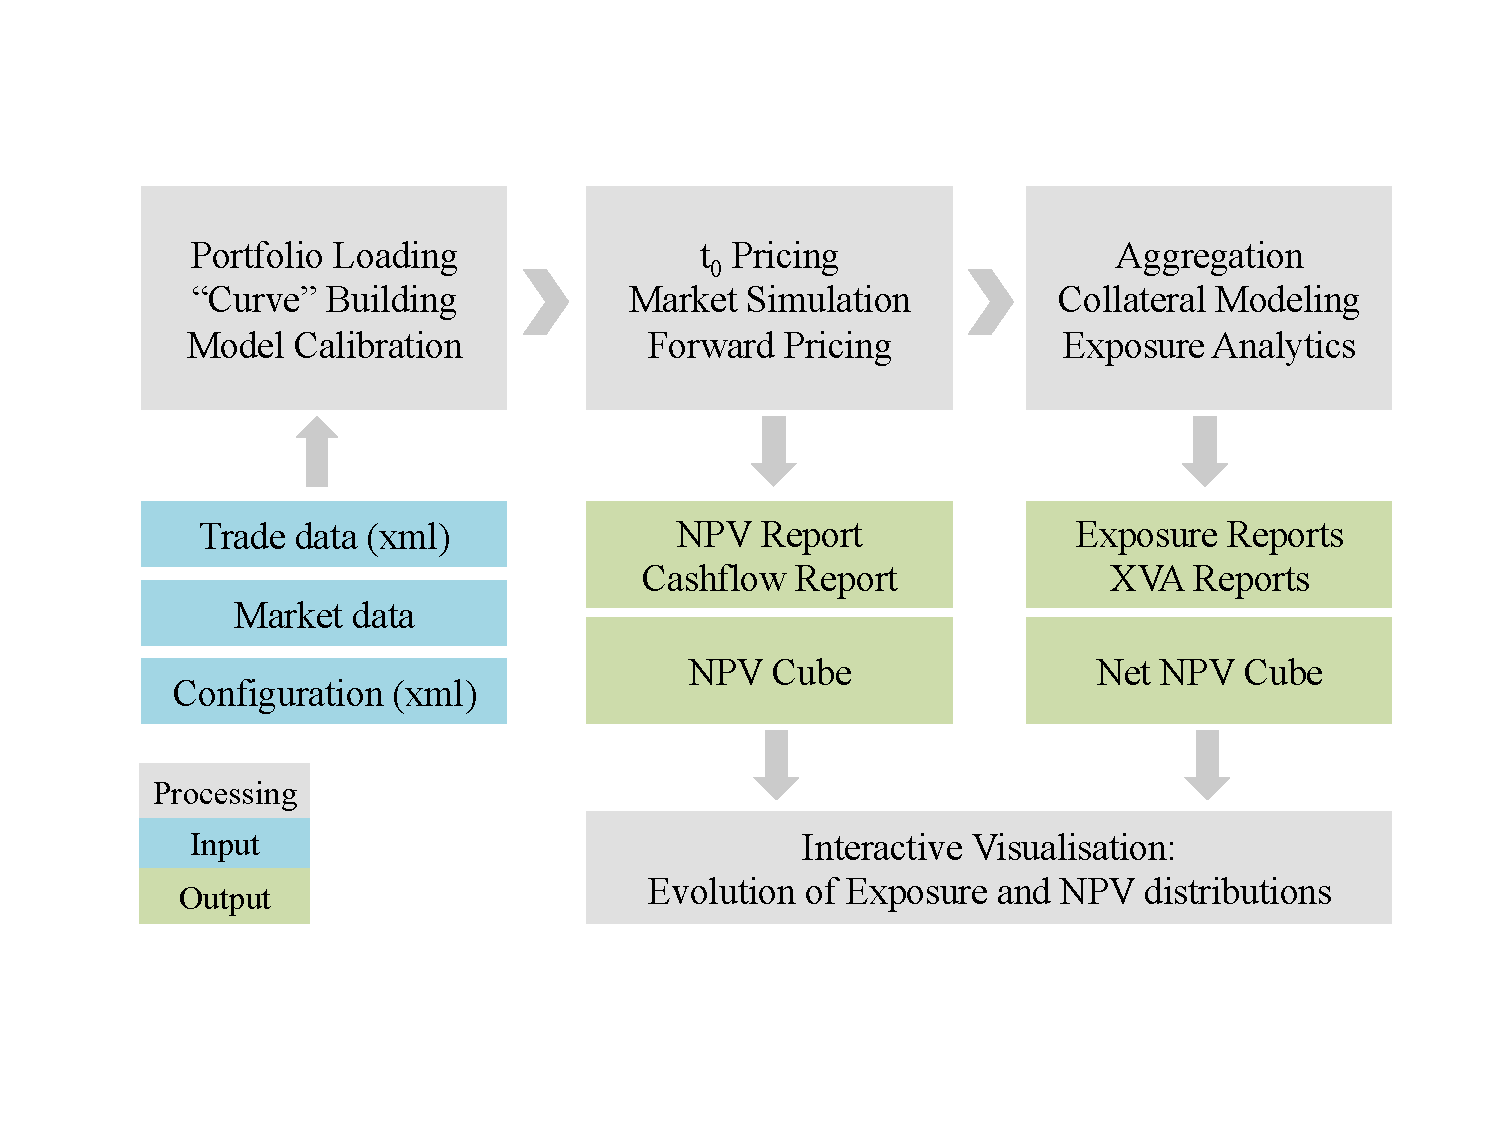
\includegraphics[scale=0.6]{process.pdf}
\end{center}
\caption{Sketch of the ORE process, inputs and outputs. }
\label{fig_process}
\end{figure}

The overall ORE process needs to be parametrised using a set of configuration XML files which is the subject of section
\ref{sec:configuration}. The portfolio is provided in XML format which is explained in detail in sections
\ref{sec:portfolio_data} and \ref{sec:nettingsetinput}. Note that ORE comes with 'Schema' files for all supported
products so that any portfolio xml file can be validated before running through ORE. Market data is provided in a simple
three-column text file with unique human-readable labelling of market data points, as explained in section
\ref{sec:market_data}.  \\

The first processing step (upper left box) then comprises 
\begin{itemize}
\item loading the portfolio to be analysed, 
\item building any yield curves or other 'term structures' needed for pricing, 
\item calibration of pricing and simulation models.
\end{itemize}

The second processing step (upper middle box) is then 
\begin{itemize}
\item portfolio valuation, cash flow generation,
\item going forward - conventional risk analysis such as sensitivity analysis and stress testing, standard-rule capital
  calculations such as SA-CCR, etc,
\item and in particular, more time-consuming, the market simulation and portfolio valuation through time under Monte
  Carlo scenarios.
\end{itemize}
This process step produces several reports (NPV, cashflows etc) and in particular an {\bf NPV cube}, i.e. NPVs per
trade, scenario and future evaluation date. The cube is written to a file in both condensed binary and human-readable
text format.  \\

The third processing step (upper right box) performs more 'sophisticated' risk ana\-ly\-sis by post-processing the NPV
cube data:
\begin{itemize}
\item aggregating over trades per netting set, 
\item applying collateral rules to compute simulated variation margin as well as simulated (dynamic) initial margin
  posting,
\item computing various XVAs including CVA, DVA, FVA, MVA for all netting sets, with and without taking collateral
  (variation and initial margin) into account, on demand with allocation to the trade level.
\end{itemize}
The outputs of this process step are XVA reports and the 'net' NPV cube, i.e. after aggregation, netting and collateral. \\

The example section \ref{sec:examples} demonstrates for representative product types how the described processing steps
can be combined in a simple batch process which produces the mentioned reports, output files and exposure evolution
graphs in one 'go'.

Moreover, both NPV cubes can be further analysed interactively using a visualisation tool introduced in section
\ref{sec:jupyter}. And finally, sections \ref{sec:calc} and \ref{sec:excel} demonstrate how ORE processes can be
launched in spreadsheets and key results presented automatically within the same sheet.

%========================================================
\section{Getting and Building ORE}\label{sec:installation}
%========================================================

You can get ORE in two ways, either by downloading a release bundle as described in section \ref{sec:release} (easiest if you just want to use ORE) or by
checking out the source code from the github repository as described in section \ref{sec:build_ore} (easiest if you want to build and develop ORE).

\subsection{ORE Releases}\label{sec:release}

ORE releases are regularly provided in the form of source code archives, Windows exe\-cutables {\tt ore.exe}, example
cases and documentation. Release archives will be provided at \url{https://github.com/opensourcerisk/engine/releases}.

The release contains the QuantLib source version that ORE depends on. This is the latest QuantLib release that precedes the ORE release including a small number of patches.

\medskip
The release consists of a single archive in zip format
\begin{itemize}
\item {\tt ORE-<VERSION>.zip}
\end{itemize}

When unpacked, it creates a directory {\tt ORE-<VERSION>} with the following files respectively subdirectories
\begin{enumerate}
%\item {\tt bin/win32/ore.exe}
%\item {\tt bin/x64/ore.exe}
\item {\tt App/}
\item {\tt Docs/}
\item {\tt Examples/}
\item {\tt FrontEnd/}
\item {\tt OREAnalytics/}
\item {\tt OREData/}
\item {\tt ORETest/}
\item {\tt QuantExt/}
\item {\tt QuantLib/}
\item {\tt ThirdPartyLibs/}
\item {\tt tools/}
\item {\tt xsd/}
\item {\tt userguide.pdf}
\end{enumerate} 

The first three items and {\tt userguide.pdf} are sufficient to run the compiled ORE application
on the list of examples described in the user guide (this works on Windows only). The Windows executables are located in {\tt App/bin/Win32/Release/} respectively {\tt App/bin/x64/Release/}. To continue with the compiled
executables:
\begin{itemize}
\item Ensure that the scripting language Python is installed on your computer, see also section \ref{sec:python}
  below;
\item Move on to the examples in section \ref{sec:examples}.
\end{itemize}

\medskip
The release bundle contains the ORE source code, which is sufficient to build ORE from sources as follows (if you build ORE for development purposes, we recommend using git though, see section \ref{sec:build_ore}):
\begin{itemize}
\item Set up Boost as described in section \ref{sec:boost}, unless already installed
\item Build QuantLib, QuantExt, OREData, OREAnalytics, App (in this order) as described in section \ref{sec:build}
\item Note that ThirdPartyLibs does not need to be built, it contains RapidXml, header only code for reading and
  writing XML files
\item Move on to section \ref{sec:python} and the examples in section \ref{sec:examples}.
\end{itemize}

Open {\tt Docs/html/index.html} to see the API documentation for QuantExt, OREData and OREAnalytics, generated by
doxygen.

\subsection{Building ORE}\label{sec:build_ore}

ORE's source code is hosted at \url{https://github.com/opensourcerisk/engine}.

\subsubsection{Git}

To access the current code base on GitHub, one needs to get {\tt git} installed first.
   
\begin{enumerate}
\item Install and setup Git on your machine following instructions at \cite{git-download}

\item Fetch ORE from github by running the following: 

{\tt\% git clone https://github.com/opensourcerisk/engine.git ore}      

This will create a folder 'ore' in your current directory that contains the codebase.

\item Initially, the QuantLib subdirectory under {\tt ore} is empty as it is a submodule pointing to the official
  QuantLib repository. To pull down locally, use the following commands:

{\tt
\% cd ore \\
\% git submodule init \\
\% git submodule update
}

\end{enumerate}

Note that one can also run 

{\footnotesize \tt\% git clone --recurse-submodules https://github.com/opensourcerisk/engine.git ore}

in step 2, which also performs the steps in 3.

\subsubsection{Boost}\label{sec:boost}

QuantLib and ORE depend on the boost C++ libraries. Hence these need to be installed before building QuantLib and
ORE. On all platforms the minimum required boost version is 1\_78.
%Other versions may work on some platforms and system configurations, but were not tested.

\subsubsection*{Windows}

\begin{enumerate}
\item Download the pre-compiled binaries for your MSVC version (e.g. MSVC-14.2 for MSVC2019) from \cite{boost-binaries}
%, any recent version should work
\begin{itemize}
\item 32-bit: \cite{boost-binaries}{\bs}VERSION{\bs}boost\_VERSION-msvc-14.2-32.exe{\bs}download 
\item 64-bit: \cite{boost-binaries}{\bs}VERSION{\bs}boost\_VERSION-msvc-14.2-64.exe{\bs}download
\end{itemize}
\item Start the installation file and choose an installation folder (the ``boost root directory''). Take a note of that folder as it will be needed later on.   
\item Finish the installation by clicking Next a couple of times.
\end{enumerate}
    
Alternatively, compile all Boost libraries directly from the source code:

\begin{enumerate}
\item Open a Visual Studio Tools Command Prompt
\begin{itemize}
\item 32-bit: VS2019 x86 Native Tools Command Prompt
\item 64-bit: VS2019 x64 Native Tools Command Prompt
\end{itemize}
\item Navigate to the boost root directory
\item Run bootstrap.bat
\item Build the libraries from the source code
\begin{itemize}
\item 32-bit: \\
  {\footnotesize\tt .{\bs}b2 --stagedir=.{\bs}lib{\bs}Win32{\bs}lib --build-type=complete toolset=msvc-14.0 \bs \\
    address-model=32 --with-test --with-system --with-filesystem  \bs \\
    --with-serialization --with-regex --with-date\_time stage}
\item 64-bit: \\
  {\footnotesize\tt .{\bs}b2 --stagedir=.{\bs}lib{\bs}x64{\bs}lib --build-type=complete toolset=msvc-14.0 \bs \\
    address-model=64 --with-test --with-system --with-filesystem \bs \\
    --with-serialization --with-regex --with-date\_time stage}
\end{itemize}
\end{enumerate}

\subsubsection*{Unix}

\begin{enumerate}
\item Download Boost from \cite{boost} and build following the instructions on the site
\item Define the environment variable BOOST that points to the boost directory
(so includes should be in BOOST and libs should be in BOOST/stage/lib)
\end{enumerate}

\subsubsection{ORE Libraries and Application}\label{sec:build}

\subsubsection*{Windows}

\begin{enumerate}

\item Download and install Visual Studio Community Edition (Version 2017 or later). 
During the installation, make sure you install the Visual
C++ support under the Programming Languages features (disabled by default).

\item Configure boost paths: \\

Set environment variables, e.g.:
\begin{itemize}
  	\item  {\tt \%BOOST\%} pointing to your directory, e.g, {\tt C:{\bs}boost\_1\_72\_0} 
  	\item {\tt \%BOOST\_LIB32\%} pointing to your Win32 lib directory, e.g, {\tt C:{\bs}boost\_1\_72\_0{\bs}lib32\-msvc\-14.2} 
	\item  {\tt \%BOOST\_LIB64\%} pointing to your x64 lib directory, e.g, {\tt C:{\bs}boost\_1\_72\_0{\bs}lib64\-msvc\-14.2} 
 \end{itemize}
 
\item Download and install CMake for Windows (https://cmake.org/download/). Visual Studio Community Edition 2019 or later supports CMake and you can install the feature 'C++ CMake Tools for Windows' instead of installing CMake as standalone program.

\end{enumerate}

%\subsubsection*{Visual Studio with CMake}

From Visual Studio 2015 and later supports CMake Projects.

\begin{enumerate}
\item Start Visual Studio 2017 or later.
\item Select "Open a local folder" from the start page or menu.
\item In the dialog window, select the ORE root directory.
\item Visual Studio will read the cmake presets from CMakePresets.json and the project file CMakeList.txt and configure the project.
\item Once the configuration is finished and one can build the project.
\item The executables are built in the subfolder {\tt /build/TARGET/CONFIGURATION/EXECUTABLE}, e.g. {\tt /build/App/Release/ore.exe}.
\end{enumerate}

ORE is shipped with configuration and build presets using Visual Studio 2022 and the Ninja build system. Those presets are configured in the CMakePreset.json which is read by Visual Studio by default when opening the CMake project. If you want to use Visual Studio 2019 or Visual Studio 2017 instead, you would have to change the Generator in the CMakePreset.json from "Visual Studio 17 2022" to "Visual Studio 16 2019" or "Visual Studio 15 2017".

You can switch in the solution explorer from the file view to the projects view, where the CMake Targets View can be selected. In this view, the various target projects can be seen below "ORE Project" and be used in a similar manner as the usual VS projects.

%\subsubsection*{Generate Visual Studio Projects with CMake}
\medskip

Alternatively, Visual Studio project files can be auto-generated from the CMake project files or ORE can be built with the CMake command line tool, similar to UNIX / Mac systems.

\begin{enumerate}

\item Generate MSVC project files from CMake files:
\begin{itemize}
\item Open a Visual Studio Tools Command Prompt
\begin{itemize}
\item 32-bit: VS2022/x86 Native Tools Command Prompt for VS 2022
\item 64-bit: VS2022/x64 Native Tools Command Prompt for VS 2022
\end{itemize}
\item Navigate to the ORE root directory
\item Run CMake command:
\begin{itemize}
\item 64-bit: \\
{\tt cmake -G "Visual Studio 17 2022" -A x64 -DBOOST\_INCLUDEDIR=\%BOOST\% -DBOOST\_LIBRARYDIR=\%BOOST\_LIB64\% -DQL\_ENABLE\_SESSIONS=ON -DMSVC\_LINK\_DYNAMIC\_RUNTIME=true -B build}
\item 32-bit: \\
{\tt cmake -G "Visual Studio 17 2022" -A x32 -DBOOST\_INCLUDEDIR=\%BOOST\% -DBOOST\_LIBRARYDIR=\%BOOST\_LIB32\% -DQL\_ENABLE\_SESSIONS=ON -DMSVC\_LINK\_DYNAMIC\_RUNTIME=true -B build}
\end{itemize}
Replace the generator "Visual Studio 17 2022" with the actual installed version.
The solution and project files will be generated in the {\tt $\langle$ORE\_ROOT$\rangle${\bs}build} subdirectory.
\end{itemize}

\item build the cmake project with the command {\tt cmake --build build -v --config Release}, 

\item or open the MSVC solution file {\tt build{\bs}ORE.sln} and build the entire solution with Visual Studio (again, make sure to select the correct platform in the configuration manager first).
\end{enumerate}

\subsubsection*{Optional: Install optional dependencies with VCPKG}

VCPKG is an open source c++ library manager. ORE can be built optionally with ZLIB and Eigen library support. 

For both features the libraries needed to be installed on the system. On Windows one can use the VCPKG package manager to install those dependencies:

\begin{itemize}
\item Install vcpkg: https://vcpkg.io/en/getting-started.html
\item Install dependencies with invoking the command \\
\medskip
{\tt vcpkg install --triplet x64-windows zlib} \\
{\tt vcpkg install --triplet x64-windows eigen3} \\
\medskip
\end{itemize}

To make VCPKG visible to CMAKE, create an environment variable {\tt VCPKG\_ROOT} pointing to the root of the vcpkg directory and configure ORE with the flag {\tt -DCMAKE\_TOOLCHAIN\_FILE=\%VCPKG\_ROOT\%/scripts/buildsystems/vcpkg.cmake}. 

To use VCPKG with Visual Studio add the toolChainFile to the configurePresets in the CMakePresets.json:

{\tt "toolchainFile": "\$env\{VCPKG\_ROOT\}/scripts/buildsystems/vcpkg.cmake",}

\subsubsection*{Unix}

With the 5th release we have discontinued automake support so that ORE can only be built with CMake on Unix systems, as follows.

\begin{enumerate}
\item set environment variable to locate the boost include and boost library directories\\
\medskip
  {\tt export BOOST\_LIB=path/to/boost/lib}\\
  {\tt export BOOST\_INC=path/to/boost/include}
\medskip
\item Change to the ORE project directory that contains the {\tt QuantLib}, {\tt QuantExt}, etc, folders; create subdirectory {\tt build} and change to subdirectory {\tt build}
\item Configure CMake by invoking \\
\medskip
{\tt cmake -DBOOST\_ROOT=\${BOOST\_INC} -DBOOST\_LIBRARYDIR=\${BOOST\_LIB} -DQL\_ENABLE\_SESSIONS=ON ..} \\
\medskip
where the {\tt QL\_ENABLE\_SESSIONS} variable is set to ON in order to enable some multi-threading applications in ORE.

Alternatively, set environment variables {\tt BOOST\_ROOT} and {\tt BOOST\_LIBRARYDIR} directly and run \\
\medskip
{\tt cmake ..} \\
\medskip
\item Build all ORE libraries, QuantLib, as well as the doxygen API documentation for QuantExt, OREData and OREAnalytics, by invoking \\
\medskip
{\tt make -j4} \\
\medskip
using four threads in this example.
\medskip
\item Run all test suites by invoking \\
\medskip
{\tt ctest -j4}
\item Run Examples (see section \ref{sec:examples})
\end{enumerate}

Note: 
\begin{itemize}
\item If the boost libraries are not installed in a standard path they might not be found during runtime because of a missing rpath
tag in their path. Run the script {\tt rename\_libs.sh} to set the rpath tag in all libraries located in {\tt
  \${BOOST}/stage/lib}.
\item Unset {\tt LD\_LIBRARY\_PATH} respectively {\tt DYLD\_LIBRARY\_PATH} before running the ORE executable or the test suites, in order not to override the rpath information embedded into the libaries built with CMake
\item On Linux systems, the 'locale' settings can negatively affect the ORE process and output. To avoid this, we
recommend setting the environment variable {\tt LC\_NUMERIC} to {\tt C}, e.g. in a bash shell, do

{\tt\footnotesize
\% export LC\_NUMERIC=C
}

before running ORE or any of the examples below. This will suppress thousand separators in numbers when converted to
strings.

\item Generate {\tt CMakeLists.txt}:

The .cpp and .hpp files included in the build process need to be explicitly specified in the various {\tt CMakeLists.txt} 
files in the project directory. The python script (in {\tt Tools/update\_cmake\_files.py}) can be used to update all CMakeLists.txt files 
automatically. 

\end{itemize}
 
\subsubsection*{ZLIB support}

To enable zlib support configure CMake with the flag {\tt -DORE\_USE\_ZLIB=ON}. 

If zlib is not installed on the system, it can be installed on Windows with the package manager VCPKG.

\subsection{Python and Jupyter}\label{sec:python}

Python (version 3.5 or higher) is required to use the ORE Python language bindings in section \ref{sec:oreswig}, 
or to run the examples in section \ref{sec:examples} and plot exposure
evolutions. Moreover, we use Jupyter \cite{jupyter} in section \ref{sec:visualisation} to visualise simulation
results. Both are part of the 'Anaconda Open Data Science Analytics Platform' \cite{Anaconda}. Anaconda installation
instructions for Windows, OS X and Linux are available on the Anaconda site, with graphical installers for
Windows\footnote{With Windows, after a fresh installation of Python the user may have to run the {\tt python} command
  once in a command shell so that the Python executable will be found subsequently when running the example scripts in
  section \ref{sec:examples}.}, Linux and OS X.

With Linux and OS X, the following environment variable settings are required
\begin{itemize}
\item set {\tt LANG} and {\tt LC\_ALL } to {\tt en\_US.UTF-8} or {\tt en\_GB.UTF-8}
\item set {\tt LC\_NUMERIC} to {\tt C}. 
\end{itemize}
The former is required for both running the Python scripts in the examples section, as well as successful installation
of the following packages. \\

The full functionality of the Jupyter notebook introduced in section \ref{sec:jupyter} requires furthermore installing
\begin{itemize}
\item jupyter\_dashboards: \url{https://github.com/jupyter-incubator/dashboards}
\item ipywidgets: \url{https://github.com/ipython/ipywidgets}
\item pythreejs: \url{https://github.com/jovyan/pythreejs}
\item bqplot: \url{https://github.com/bloomberg/bqplot}
\end{itemize}
With Python and Anaconda already installed, this can be done by running these commands
\begin{itemize}
\item {\tt conda install -c conda-forge ipywidgets}
\item {\tt pip install jupyter\_dashboards}
\item {\tt jupyter dashboards quick-setup --sys-prefix}
\item {\tt conda install -c conda-forge bqplot}
\item {\tt conda install -c conda-forge pythreejs}
\end{itemize}
Note that the bqplot installation requires the environment settings mentioned above.

\subsection{Building ORE-SWIG and Python Wheels}\label{sec:oreswig}

Since release 4, ORE comes with Python and Java language bindings following the QuantLib-SWIG example.
The ORE bindings extend the QuantLib SWIG wrappers and allow calling ORE functionality in the 
QuantExt/OREData/OREAnalytics libraries alongside with functionality in QuantLib.  

\medskip
The ORE-SWIG source code is hosted in a separate git repository at \url{https://github.com/opensourcerisk/ore-swig}.
The {\tt README.md} in the top level directory of this git repository contains build instructions and refers to tutorials 
for installing and building Python wrappers and wheels.

\medskip
Typical usage of the Python wrapper is shown in ORE's {\tt Example\_42} and in ORE SWIG's {\tt OREAnalytics/Python/Examples} directory.

%
%\medskip
%To build the wrappers on Windows, Linux, mac OS
%\begin{enumerate}
%\item build ORE and QuantLib first, as shown in the previous section. It is strongly advised to switch the codebase to a release tag here (e.g. 1.8.7.0), as the versions of the master branch are not always aligned!
%\item check out the ORE-SWIG repository into a project directory {\tt oreswig}, change into that directory (the same advice as above applies here as well, switch to the same release tag as ORE)
%\item pull in the QuantLib-SWIG project by running \\
%{\tt git submodule init} \\
%{\tt git submodule update}
%%\item Edit the top-level {\tt oreswig/CMakeLists.txt} and uncomment e.g. the line {\tt add\_subdirectory(OREAnalytics-SWIG/Python)} to build the OREAnalytics Python wrappers
%\item Create a subdirectory {\tt build}, change into that directory and configure cmake and then build using Ninja as follows \\
%\medskip
%{\footnotesize
%{\tt cmake -G Ninja $\backslash$} \\
%\hspace{1cm} {\tt -D ORE=<ORE Root Directory> $\backslash$} \\
%\hspace{1cm} {\tt -D BOOST\_ROOT=<Top level boost include directory> $\backslash$}\\
%\hspace{1cm} {\tt -D BOOST\_LIBRARYDIR=<Location of the compiled boost libraries> $\backslash$}\\
%\hspace{1cm} {\tt -D Python\_ROOT\_DIR=<Root directory of the python installation>$\backslash$} \\
%\hspace{1cm} {\tt ..} \\
%{\tt ninja} \\
%}
%\medskip
%On Linux or mac OS one can also use {\tt make} instead of {\tt ninja}. 
%In that case, omit the {\tt -G Ninja} part in the configuration. 
%
%\medskip
%To build on Windows using CMake and an existing Visual Studio installation you can e.g. run
%this from the top-level oreswig directory
%
%{\footnotesize
%{\tt mkdir build $\backslash$} \\
%{\tt cmake -G "Visual Studio 15 2017" $\backslash$}\\
%\hspace{1cm} {\tt -A x64 $\backslash$}\\
%\hspace{1cm} {\tt -D SWIG\_DIR=C:$\backslash$dev$\backslash$swigwin$\backslash$Lib $\backslash$}\\
%\hspace{1cm} {\tt -D SWIG\_EXECUTABLE=C:$\backslash$dev$\backslash$swigwin$\backslash$swig.exe $\backslash$}\\
%\hspace{1cm} {\tt -D ORE:PATHNAME=C:$\backslash$dev$\backslash$ORE$\backslash$master $\backslash$}\\
%\hspace{1cm} {\tt -D BOOST\_ROOT=C:$\backslash$dev$\backslash$boost $\backslash$}\\
%\hspace{1cm} {\tt -S OREAnalytics-SWIG/Python $\backslash$}\\
%\hspace{1cm} {\tt -B build $\backslash$}\\
%{\tt cmake -{}-build build -v}
%}

%\medskip
%
%This builds the OREAnalytics-Python bindings which include the wrapped parts of QuantLib, QuantExt, OREData and OREAnalytics.
%
%\begin{itemize}
%\item Try a Python example: Update your PYTHONPATH environment variable to include directory {\tt oreswig/build/OREAnalytics-SWIG/Python} 
%which contains both the new python module and the associated native library loaded by the python module;
%change to the {\tt oreswig/OREAnalytics/Python/Examples} directory and run e.g.\\
%
%\medskip
%\centerline{\tt python ore.py}  
%
%There is also an IPython example in the same directory. To try it, launch 
%
%\medskip
%\centerline{\tt jupyter notebook}  
%
%wait for your browser to open, select {\tt ore.ipy} from the list of files and then run all cells.
%
%\item Try a Java example: Make sure that the line {\tt add\_subdirectory(OREAnalytics-SWIG/Java)} 
%is uncommented in the top-level CMakeLists.txt file when building; change to directory 
%{\tt ORE-SWIG/OREAnalytics-SWIG/Java/Examples} and run
%
%\medskip
%{\tt java -Djava.library.path=../../../build/OREAnalytics-SWIG/Java $\backslash$} \\
%\hspace{1cm} {\tt -jar ../../../build/OREAnalytics-SWIG/Java/ORERunner.jar $\backslash$}\\
%\hspace{1cm} {\tt Input/ore.xml}
%
%\end{enumerate}
%
%\subsection{How to build ORE Python Wheels on Windows}\label{sec:win_wheel}
%
%This section is a stand-alone HOWTO for building ore and oreswig, including Python wrappers and wheels, at the DOS command line using cmake and VS 2022.  
%
%\subsubsection*{Prerequisites}
% 
%\begin{itemize}
%\item python: The following tools need to be up to date: \\
% {\tt python -m ensurepip } \\
% {\tt pip install build }
%\item boost: Download the binaries from the link below.  This release was tested against boost version 1.72.  It is important to download these precompiled binaries (rather than compiling yourself from source code) because the binaries include ZLIB support which this build requires. \\
%\url{https://sourceforge.net/projects/boost/files/boost-binaries}
%\item  swig: You need to either install the binaries, or install the source code and build yourself
% \item ore and oreswig: You need to install the source code. Instructions for building with cmake are provided below.
% \end{itemize}
% 
%\subsubsection*{Environment variables}
% 
%Set the following environment variables to the paths where the above items live on your machine, e.g:
% 
%{\tt set BOOST\_INC=C:{\bs}repos{\bs}boost{\bs}boost\_1\_81\_0} \\
%{\tt set BOOST\_LIB=C:{\bs}repos{\bs}boost{\bs}boost\_1\_81\_0{\bs}lib{\bs}x64{\bs}lib} \\
%{\tt set SWIG=C:{\bs}repos{\bs}swigwin-4.1.1} \\
%{\tt set ORE=C:{\bs}repos{\bs}ore } \\
%{\tt set ORESWIG=C:{\bs}repos{\bs}oreswig}
% 
%\subsubsection*{Build ORE}
% 
%Generate the project files:
% 
%\medskip
%{\tt cd \%ORE\%} \\
%{\tt mkdir build }\\
%{\tt cd \%ORE\%{\bs}build} \\
%{\tt cmake .. $\backslash$\\
%\hspace{1cm} -DBoost\_NO\_WARN\_NEW\_VERSIONS=1 $\backslash$\\
%\hspace{1cm} -Wno-dev -G "Visual Studio 17 2022" $\backslash$ \\
%\hspace{1cm} -A x64 $\backslash$\\
%\hspace{1cm} -DMSVC\_LINK\_DYNAMIC\_RUNTIME=OFF $\backslash$ \\
%\hspace{1cm} -DBOOST\_ROOT=\$BOOST\_INC $\backslash$\\
%\hspace{1cm} -DBOOST\_LIBRARYDIR=\$BOOST\_LIB $\backslash$ \\
%\hspace{1cm} -DQL\_ENABLE\_SESSIONS=ON} 
%
%\medskip
%This will create \%ORE\%{\bs}build{\bs}ORE.sln
% 
%\medskip
%Build:
% 
%\medskip
%{\tt cd \%ORE\%{\bs}build} \\
%%{\tt "C:{\bs}Program Files{\bs}CMake{\bs}bin{\bs}cmake.exe" -{}-build . -{}-config Release}
%{\tt cmake -{}-build . -{}-config Release}
%
%\medskip
%This will create  \%ORE\%{\bs}build{\bs}OREAnalytics{\bs}orea{\bs}Release{\bs}OREAnalytics-x64-mt.lib
% 
%\subsubsection*{Build ORE-SWIG Wrapper and Wheel}
% 
%In contrast to the generic cmake-based SWIG build in section \ref{sec:oreswig}, we are now resorting to python's setup.py.
% 
%\medskip
%{\tt cd \%ORESWIG\%{\bs}OREAnalytics-SWIG{\bs}Python} \\
%{\tt set BOOST\_ROOT=\%BOOST\_INC\%} \\
%% set BOOST_LIB is needed but already done above
%% set ORE needed but already done above
%{\tt set PATH=\%PATH\%;\%SWIG\%} \\
%{\tt set ORE\_STATIC\_RUNTIME=1} \\
%{\tt python setup.py wrap} \\
%{\tt python setup.py build} \\
%{\tt python setup.py test} \\
%{\tt python -m build -{}-wheel} 
% 
%\medskip
%This will create 
%\begin{itemize}
%\item the Python module and static library in folder {\tt <PATH>{\bs}build{\bs}lib.win-amd64-cpython-310} (the directory name depends on the machine and python version)
%\item the wheel file (filename.whl) in folder {\tt <PATH>{\bs}dist}
%\end{itemize}
%where {\tt <PATH>} stands for {\tt \%ORESWIG\%{\bs}OREAnalytics-SWIG{\bs}Python}.
%
%\medskip
%To use the wrapper directly: \\
%\medskip
%{\tt cd <PATH>{\bs}Examples} \\
%{\tt set PYTHONPATH=<PATH>{\bs}build{\bs}lib.win-amd64-cpython-310} \\
%{\tt python swap.py}
%
%\medskip
%To use the wheel:
% 
%{\tt cd <PATH>{\bs}Examples} \\
%{\tt python -m venv env1} \\
%{\tt .{\bs}env1{\bs}Scripts{\bs}activate.bat} \\
%{\tt pip install <PATH>{\bs}dist{\bs}filename.whl} \\
%{\tt python swap.py} \\
%{\tt deactivate} \\
%{\tt rmdir /s /q env1} \\
%
%\subsection{How to build ORE Python Wheels on Linux and macOS}\label{sec:nix_wheel}
%
%This section is a stand-alone HOWTO for building and using a python wheel for OREAnalytics on Linux or macOS.
%
%\subsubsection*{Prerequisites}
%
%\begin{itemize}
%\item python: Ensure that python3, pip, build, and virtualenv are installed and up to date. \\
%
%\medskip
%For example, on ubuntu:\\
%{\tt sudo apt install python3-pip} \\
%{\tt sudo apt install python3.10-venv} \\
%{\tt pip3 install -{}-upgrade build} \\
%
%\medskip
%On macOS it is recommended to install jupyterlab (which contains python and pip) with \\
%{\tt brew install jupyterlab} \\
%followed by\\
%{\tt pip install -{}-upgrade build} \\
%{\tt pip install virtualenv} 
%
%\item python3-dev: You need to install the python header files and libs. On some platforms these come already installed with python.  
%
%\medskip
%On ubuntu they do not and the command to install them is: \\
%{\tt sudo apt install python3-dev }\\
%
%\medskip
%On macOS they come with the recommended installation of jupyterlab
%
%\item boost and swig: You need to either install the binaries, or install the source code and build yourself.
%\item ore and oreswig: You need to install the source code. Instructions for building with cmake are provided below.
%\end{itemize}
%
%\subsubsection*{Environment variables}
%
%Set the following environment variables to the paths where the ore and ore swig repos, as well as boost live on your machine, e.g:
%
%\medskip
%{\tt export ORE=\$HOME/dev/ore} \\
%{\tt export ORESWIG=\$HOME/dev/oreswig}\\
%{\tt export BOOST\_INC=/opt/homebrew/include} \\
%{\tt export BOOST\_LIB=/opt/homebrew/lib} 
%
%\subsubsection*{Build ORE}
%
%Use cmake to generate the project Makefiles
%
%\medskip
%{\tt cd \$ORE} \\
%{\tt mkdir build} \\
%{\tt cd \$ORE/build} \\
%{\tt cmake .. \\
%\hspace{1cm} -DQL\_ENABLE\_SESSIONS=ON $\backslash$\\
%\hspace{1cm} -DCMAKE\_POSITION\_INDEPENDENT\_CODE=ON $\backslash$\\
%\hspace{1cm} -DORE\_BUILD\_DOC=OFF $\backslash$ \\
%\hspace{1cm} -DORE\_BUILD\_EXAMPLES=OFF $\backslash$ \\
%\hspace{1cm} -DORE\_BUILD\_TESTS=OFF $\backslash$\\
%\hspace{1cm} -DORE\_BUILD\_APP=OFF $\backslash$\\
%\hspace{1cm} -DQL\_BUILD\_BENCHMARK=OFF $\backslash$\\
%\hspace{1cm} -DQL\_BUILD\_EXAMPLES=OFF $\backslash$\\
%\hspace{1cm} -DQL\_BUILD\_TEST\_SUITE=OFF $\backslash$\\
%\hspace{1cm} -DBoost\_NO\_WARN\_NEW\_VERSIONS=1 $\backslash$\\
%\hspace{1cm} -DBoost\_NO\_SYSTEM\_PATHS=1 $\backslash$\\
%\hspace{1cm} -DBOOST\_ROOT=\$BOOST\_INC $\backslash$\\
%\hspace{1cm} -DBOOST\_LIBRARYDIR=\$BOOST\_LIB}
%
%\medskip
%Execute the following to kick off the build:
%
%\medskip
%{\tt cd \$ORE/build} \\
%{\tt cmake -{}-build} . 
%
%\medskip
%This will generate \$ORE/build/OREAnalytics/orea/libOREAnalytics.so or .dylib
%
%\subsubsection*{Build ORE-SWIG Wrapper and Wheel}
%
%In contrast to the generic cmake-based SWIG build in section \ref{sec:oreswig}, we are now resorting to python's setup.py. 
%
%The commands below will try to link to boost library boost\_thread.  On some platforms this lib has a different name and if that is the case for you then you can override it, e.g:
%
%{\tt export BOOST\_THREAD=boost\_thread-mt} \\
%
%\medskip
%
%Ensure that environent variables ORE, BOOST\_INC and BOOST\_LIB are set (see above), then
%
%\medskip
%{\tt cd \$ORESWIG/OREAnalytics-SWIG/Python} \\
%{\tt python setup.py wrap} \\
%{\tt python setup.py build} \\
%{\tt python -m build -{}-wheel}
%
%\medskip
%will then generate the wheel file (filename.whl) in folder \$ORESWIG/OREAnalytics-SWIG/Python/dist.
%For the second step above you may need to modify the \$ORESWIG/OREAnalytics-SWIG/oreanalytics-config script to return the appropriate cflags and libs on your machine.
%
%\medskip
%To use the wheel:
%
%\medskip
%{\tt cd \$ORESWIG/OREAnalytics-SWIG/Python/Examples} \\
%{\tt python -m venv env1} \\
%{\tt . ./env1/bin/activate} \\
%{\tt pip install \$ORESWIG/OREAnalytics-SWIG/Python/dist/filename.whl} \\
%{\tt python commodityforward.py} \\
%{\tt deactivate} \\
%{\tt rm -rf env1}

%========================================================
\section{Examples}\label{sec:examples}
%========================================================

The examples shown in table \ref{tab_0} are intended to help with getting started with ORE, and to serve as plausibility
checks for the simulation results generated with ORE.

\begin{table}[hbt]
\scriptsize
\begin{center}
\begin{tabular}{|c|l|}
\hline
Example & Description \\
\hline
\hline
1 & Vanilla at-the-money Swap with flat yield curve \\
\hline
2 & Vanilla Swap with normal yield curve \\
\hline
3 & European Swaption \\
\hline
4 & Bermudan Swaption \\
\hline
5 & Callable Swap \\
\hline
6 & Cap/Floor \\
\hline
7 & FX Forward \\
  & European FX Option \\ 
\hline
8 & Cross Currency Swap without notional reset \\
\hline
9 & Cross Currency Swap with notional reset \\
\hline
10 & Three-Swap portfolio with netting and collateral \\
   & XVAs - CVA, DVA, FVA, MVA, COLVA \\
   & Exposure and XVA Allocation to trade level \\
\hline
11 & Basel exposure measures - EE, EPE, EEPE \\
\hline
12 & Long term simulation with horizon shift \\
\hline
13 & Dynamic Initial Margin and MVA \\
\hline
14 & Minimal Market Data Setup \\
\hline
15 & Sensitivity Analysis and Stress Testing \\
\hline
16 & Equity Derivatives Exposure \\
\hline
17 & Inflation Swap Exposure under Dodgson-Kainth\\
\hline
18 & Bonds and Amortisation Structures\\
\hline
19 & Swaption Pricing with Smile\\
\hline
20 & Credit Default Swap Pricing\\
\hline
21 & Constant Maturity Swap Pricing\\
\hline
22 & Option Sensitivity Analysis with Smile\\
\hline
23 & Forward Rate Agreement and Averaging OIS Exposure\\
\hline
24 & Commodity Forward and Option Pricing and Sensitivity\\
\hline
25 & CMS Spread with (Digital) Cap/Floor Pricing, Sensitivity and Exposures\\
\hline
26 & Bootstrap Consistency\\
\hline
27 & BMA Basis Swap Pricing and Sensitivity\\
\hline
28 & Discount Ratio Curves\\
\hline
29 & Curve Building using Fixed vs. Float Cross Currency Helpers\\
\hline
30 & USD-Prime Curve Building via Prime-LIBOR Basis Swap\\
\hline
31 & Exposure Simulation using a Close-out Grid\\
\hline
32 & Inflation Swap Exposure under Jarrow-Yildrim\\ 
\hline
33 & CDS Exposure Simulation \\
\hline
34 & Wrong Way Risk \\
\hline
35 & Flip View \\
\hline
36 & Choice of Measure \\
\hline
37 & Multifactor Hull-White scenario generation \\
\hline
38 & Cross Currency Exposure using Multifactor Hull-White Models \\
\hline
39 & Exposure Simulation using American Monte Carlo \\
\hline
40 & Par Sensitivity Analysis \\
\hline
41 & Multi-threaded Exposure Simulation \\
\hline
42 & ORE Python Module \\
\hline
43 & Credit Portfolio Model \\
\hline
44 & ISDA SIMM Model \\
\hline
45 & Collateralized Bond Obligation \\
\hline
46 & Generic Total Return Swap \\
\hline
47 & Composite Trade \\
\hline
48 & Convertible Bond and ASCOT \\
\hline
49 & Bond Yield Shifted \\
\hline
50 & Par Sensitivity Conversion of external "Raw" Sensis \\
\hline
51 & Custom Trade Fixings\\
\hline
52 & Scripted Trades \\
\hline
\end{tabular}
\caption{ORE examples.}
\label{tab_0}
\end{center}
\end{table}
\clearpage

All example results can be produced with the Python scripts {\tt run.py} in the ORE release's {\tt Examples/Example\_\#}
folders which work on both Windows and Unix platforms. In a nutshell, all scripts call ORE's command line application
with a single input XML file

\medskip
\centerline{\tt ore[.exe] ore.xml}
\medskip

They produce a number of standard reports and exposure graphs in PDF format. The structure of the input file and of the
portfolio, market and other configuration files referred to therein will be explained in section
\ref{sec:configuration}.

\medskip ORE is driven by a number of input files, listed in table \ref{tab_1} and explained in detail in sections
\ref{sec:configuration} to \ref{sec:fixings}. In all examples, these input files are either located in the example's sub
directory {\tt Examples/Example\_\#/Input} or the main input directory {\tt Examples/Input} if used across several
examples. The particular selection of input files is determined by the 'master' input file {\tt ore.xml}.

\begin{table}[h]
\scriptsize
\begin{center}
\begin{tabular}{|l|p{11cm}|}
  \hline
  File Name & Description \\
  \hline
  {\tt ore.xml}&   Master input file, selection of further inputs below and selection of analytics \\
  {\tt portfolio.xml} & Trade data \\
  {\tt netting.xml} &  Collateral (CSA) data \\
  {\tt simulation.xml} & Configuration of simulation model and market\\
  {\tt market.txt} &  Market data snapshot \\
  {\tt fixings.txt} &  Index fixing history \\
  {\tt dividends.txt} &  Dividends history \\
  {\tt curveconfig.xml} & Curve and term structure composition from individual market instruments\\
  {\tt conventions.xml} & Market conventions for all market data points\\
  {\tt todaysmarket.xml} &  Configuration of the market composition, relevant for the pricing of the given portfolio as
                           of today (yield curves, FX rates, volatility surfaces etc) \\
  {\tt pricingengines.xml} &  Configuration of pricing methods by product\\
  \hline
\end{tabular}
\end{center}
\caption{ORE input files}
\label{tab_1}
\end{table}

The typical list of output files and reports is shown in table \ref{tab_2}. The names of output files can be configured
through the master input file {\tt ore.xml}. Whether these reports are generated also depends on the setting in {\tt
  ore.xml}. For the examples, all output will be written to the directory {\tt Examples/Example\_\#/Output}.

\begin{table}[h]
\scriptsize
\begin{center}
\begin{tabular}{|l|p{11cm}|}
\hline
File Name & Description \\
\hline
{\tt npv.csv}&   NPV report \\
{\tt flows.csv} & Cashflow report \\
{\tt curves.csv} & Generated yield (discount) curves report \\
{\tt xva.csv} & XVA report, value adjustments at netting set and trade level \\
{\tt exposure\_trade\_*.csv} & Trade exposure evolution reports\\
{\tt exposure\_nettingset\_*.csv} &  Netting set exposure evolution reports\\
{\tt rawcube.csv} & NPV cube in readable text format \\
{\tt netcube.csv} & NPV cube after netting and colateral, in readable text format \\
{\tt *.csv.gz} & Intermediate storage of NPV cube and scenario data \\
{\tt *.pdf} &  Exposure graphics produced by the python script {\tt run.py} after ORE completed\\
\hline
\end{tabular}
\end{center}
\caption{ORE output files}
\label{tab_2}
\end{table}

Note: When building ORE from sources on Windows platforms, make sure that you copy your {\tt ore.exe} to the binary
directory {\tt App/bin/win32/} respectively {\tt App/bin/x64/}. Otherwise the examples may be run using the pre-compiled
executables which come with the ORE release.

%--------------------------------------------------------
\subsection{Interest Rate Swap Exposure, Flat Market}\label{sec:example1}
%--------------------------------------------------------

We start with a vanilla single currency Swap (currency EUR, maturity 20y, notional 10m, receive fixed 2\% annual, pay
6M-Euribor flat). The market yield curves (for both discounting and forward projection) are set to be flat at 2\% for
all maturities, i.e. the Swap is at the money initially and remains at the money on average throughout its life. Running
ORE in directory {\tt Examples/Example\_1} with

\medskip
\centerline{\tt python run.py } 
\medskip

yields the exposure evolution in 

\medskip
\centerline{\tt Examples/Example\_1/Output/*.pdf } 
\medskip

and shown in figure \ref{fig_1}. 
\begin{figure}[h!]
\begin{center}
%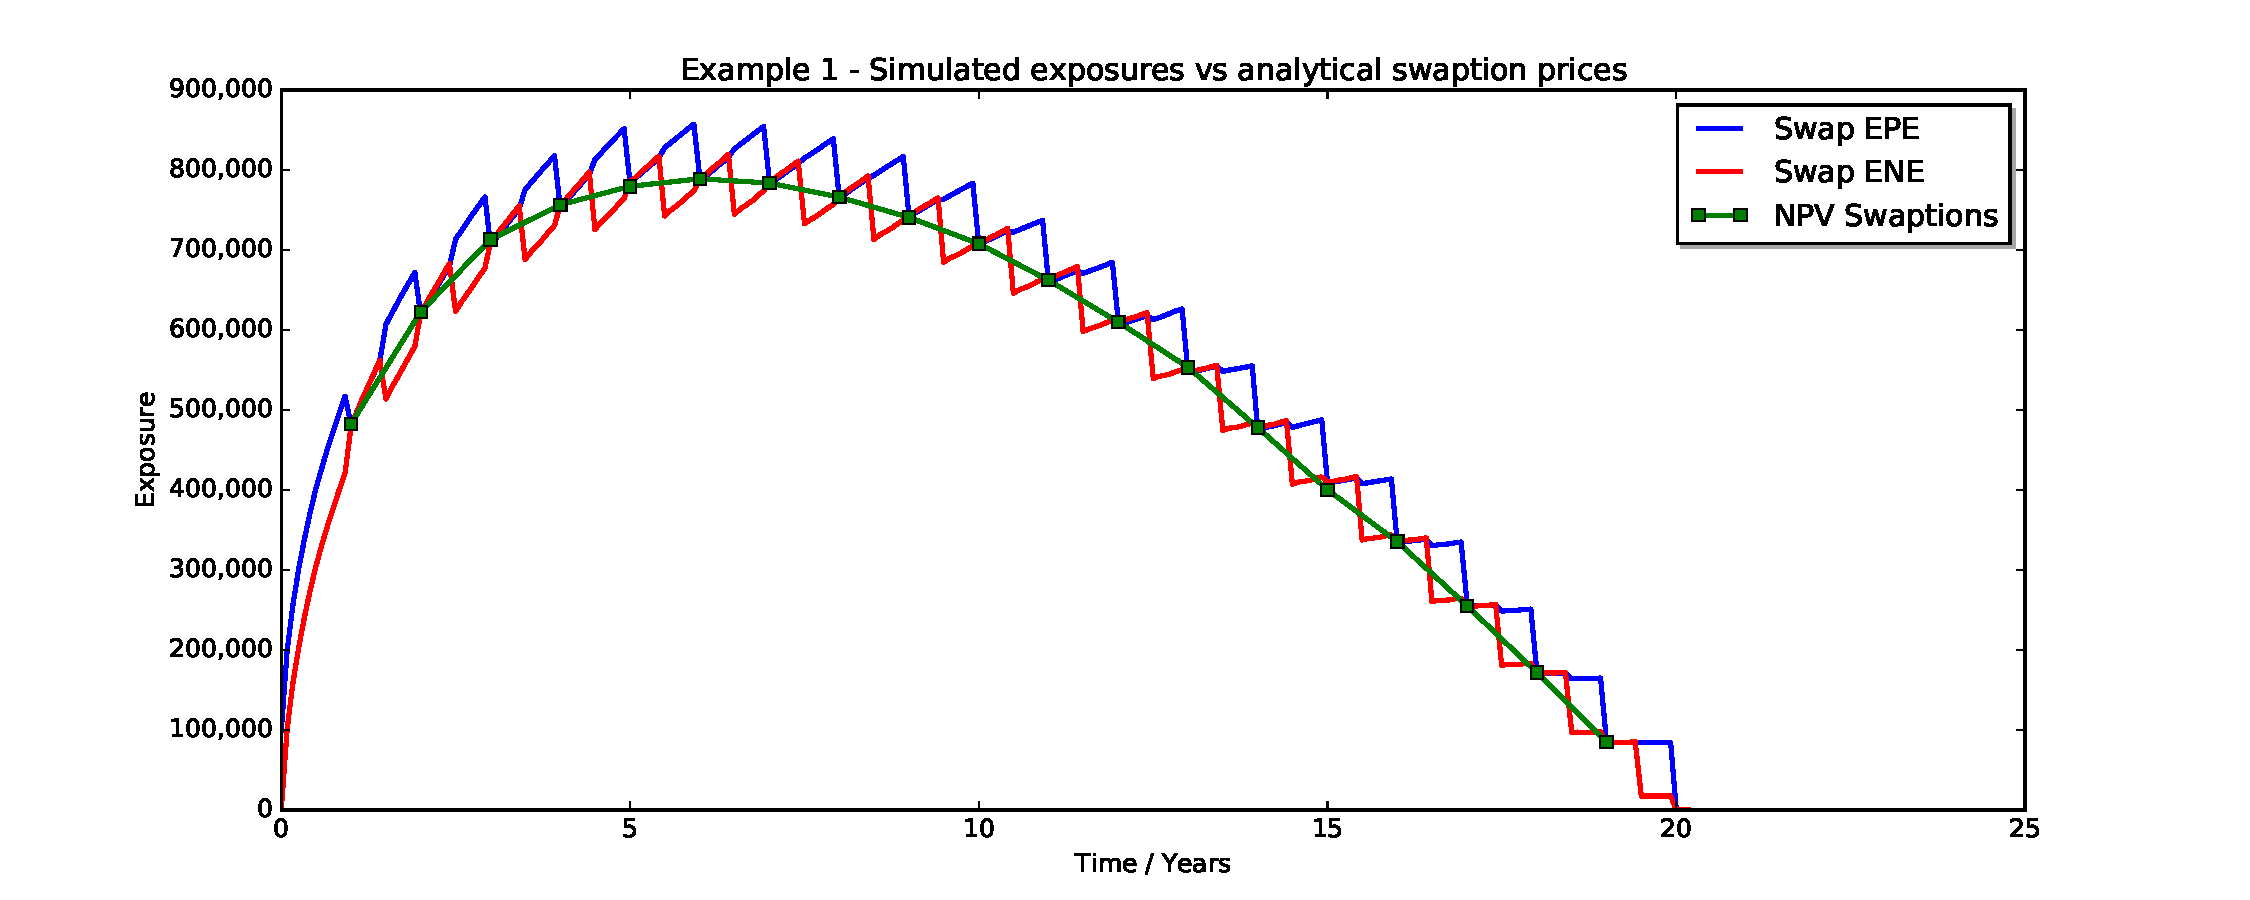
\includegraphics[scale=0.45]{mpl_swap_1_1m_sbb_100k.pdf}
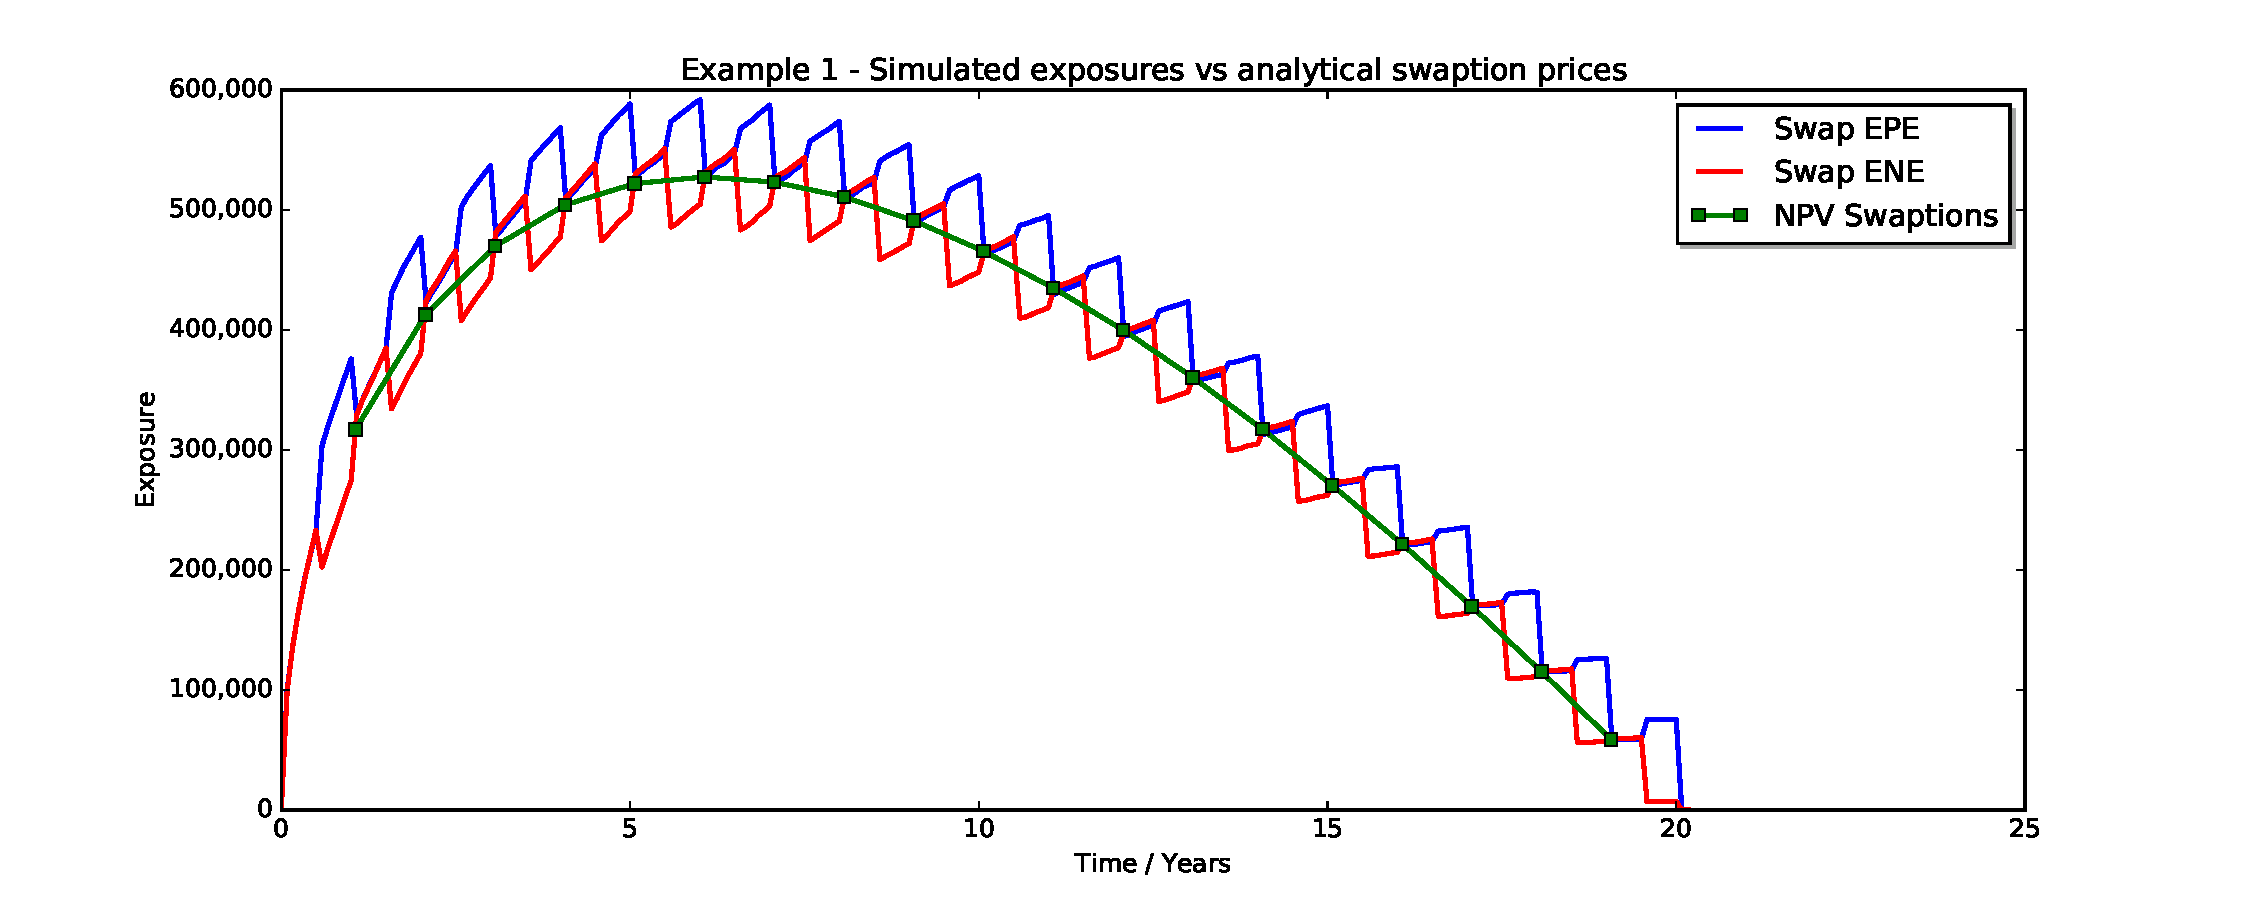
\includegraphics[scale=0.45]{mpl_swap_1_1m_sbb_10k_flat.pdf}
\end{center}
\caption{Vanilla ATM Swap expected exposure in a flat market environment from both parties' perspectives. The symbols are European Swaption prices. The simulation was run with monthly time steps and 10,000 Monte Carlo samples to demonstrate the convergence of EPE and ENE profiles. A similar
outcome can be obtained more quickly with 5,000 samples on a quarterly time grid which is the default setting of Example\_1. }
\label{fig_1}
\end{figure}
Both Swap simulation and Swaption pricing are run with calls to the ORE executable, essentially 

\medskip
\centerline{\tt ore[.exe] ore.xml} 

\centerline{\tt ore[.exe] ore\_swaption.xml} 
\medskip

which are wrapped into the script {\tt Examples/Example\_1/run.py} provided with the ORE release.
It is instructive to look into the input folder in Examples/Example\_1, the content of the main input file {\tt
  ore.xml}, together with the explanations in section \ref{sec:configuration}. \\

This simple example is an important test case which is also run similarly in one of the unit test suites of ORE. The
expected exposure can be seen as a European option on the underlying netting set, see also appendix
\ref{sec:app_exposure}. In this example, the expected exposure at some future point in time, say 10 years, is equal to
the European Swaption price for an option with expiry in 10 years, underlying Swap start in 10 years and underlying Swap
maturity in 20 years. We can easily compute such standard European Swaption prices for all future points in time where
both Swap legs reset, i.e. annually in this case\footnote{Using closed form expressions for standard European Swaption
  prices.}. And if the simulation model has been calibrated to the points on the Swaption surface which are used for
European Swaption pricing, then we can expect to see that the simulated exposure matches Swaption prices at these annual
points, as in figure \ref{fig_1}.  In Example\_1 we used co-terminal ATM Swaptions for both model calibration and
Swaption pricing. Moreover, as the yield curve is flat in this example, the exposures from both parties'
perspectives (EPE and ENE) match not only at the annual resets, but also for the period between annual reset of both
legs to the point in time when the floating leg resets. Thereafter, between floating leg (only) reset and next joint
fixed/floating leg reset, we see and expect a deviation of the two exposure profiles.

%--------------------------------------------------------
\subsection{Interest Rate Swap Exposure, Realistic Market}\label{sec:example2}
%--------------------------------------------------------

Moving to {\tt Examples/Example\_2}, we see what changes when using a realistic (non-flat) market
environment. Running the example with

\medskip
\centerline{\tt python run.py } 
\medskip

yields the exposure evolution in 

\medskip
\centerline{\tt Examples/Example\_2/Output/*.pdf } 
\medskip

shown in figure \ref{fig_2}.
\begin{figure}[h!]
\begin{center}
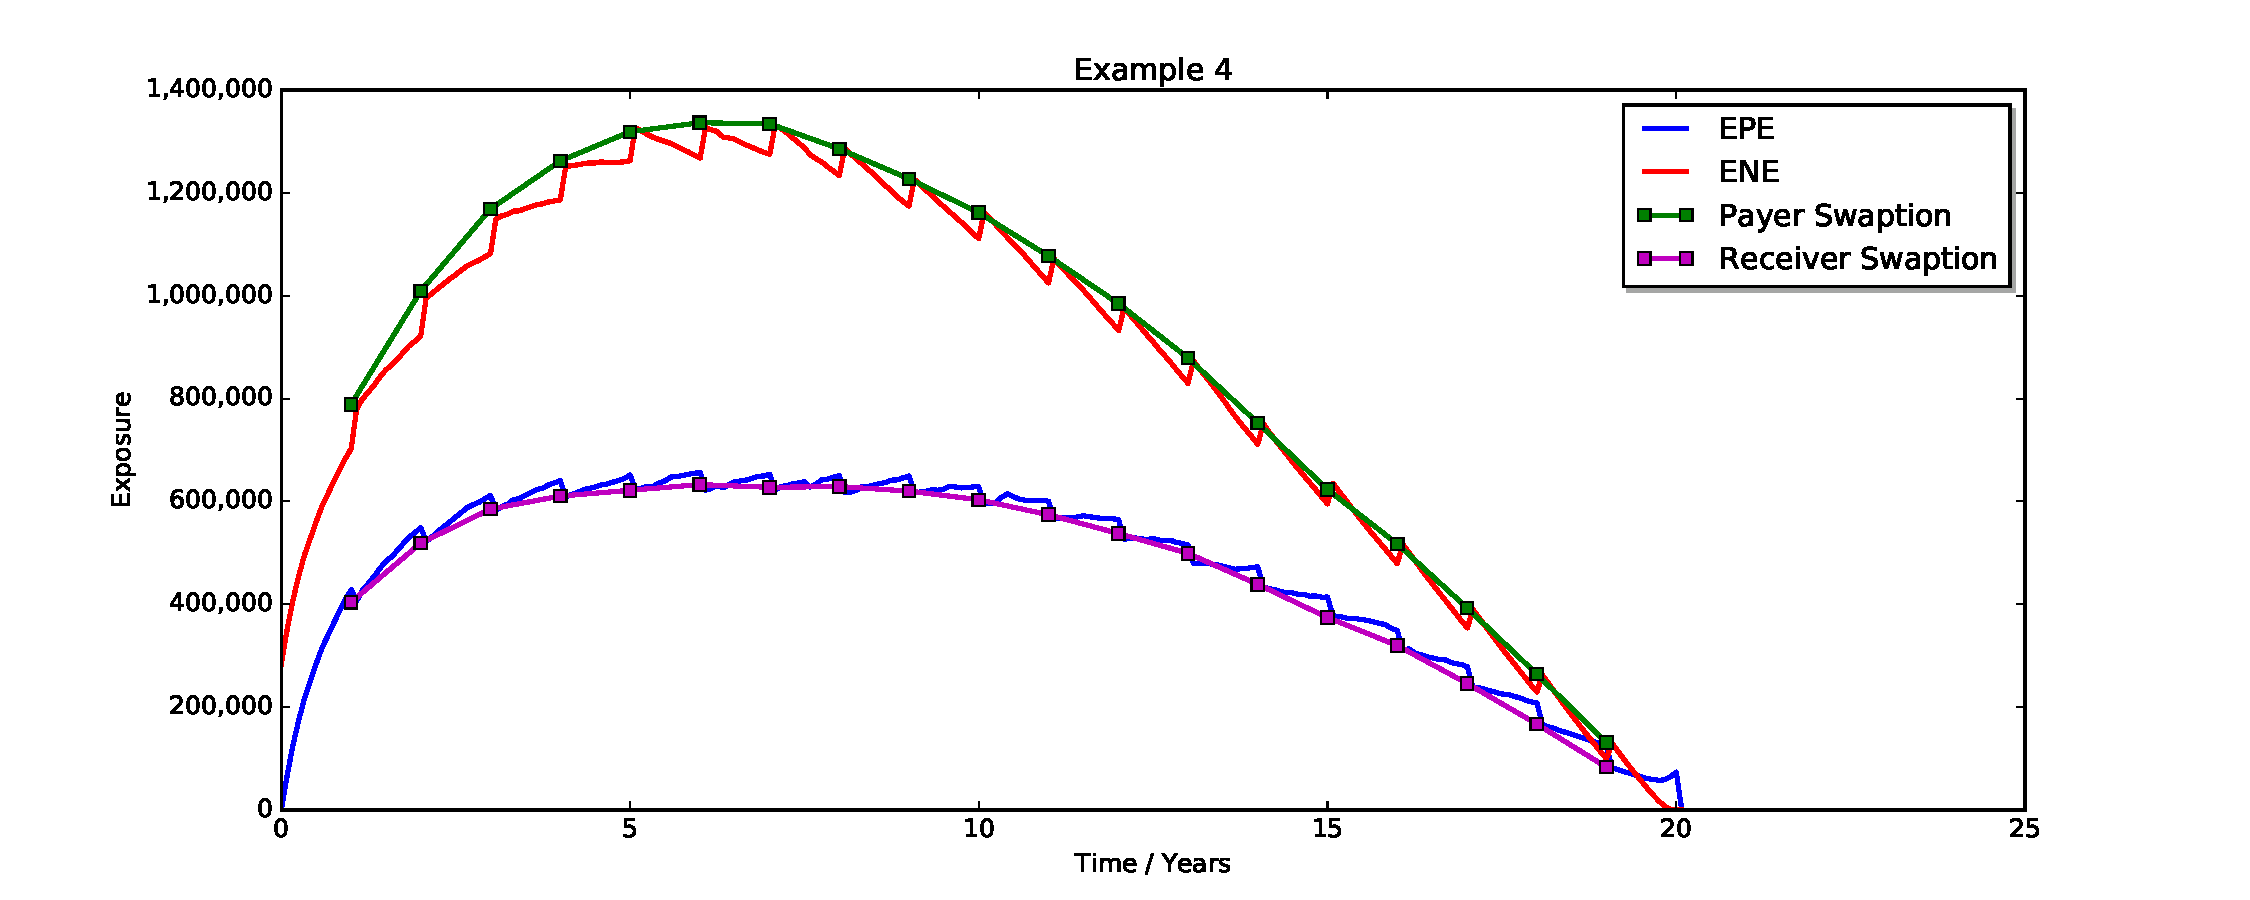
\includegraphics[scale=0.45]{mpl_swap_3.pdf}
\end{center}
\caption{Vanilla ATM Swap expected exposure in a realistic market environment as of 05/02/2016 from both parties'
  perspectives. The Swap is the same as in figure \ref{fig_1} but receiving fixed 1\%, roughly at the money. The symbols
  are the prices of European payer and receiver Swaptions. Simulation with 5000 paths and monthly time steps.}
\label{fig_2}
\end{figure}
In this case, where the curves (discount and forward) are upward sloping, the receiver Swap is at the money at inception
only and moves (on average) out of the money during its life. Similarly, the Swap moves into the money from the
counterparty's perspective. Hence the expected exposure evolutions from our perspective (EPE) and the counterparty's
perspective (ENE) 'detach' here, while both can still be be reconciled with payer or respectively receiver Swaption
prices.

%--------------------------------------------------------
\subsection{European Swaption Exposure}\label{sec:european_swaption}
%--------------------------------------------------------

This demo case in folder {\tt Examples/Example\_3} shows the exposure evolution of European Swaptions with cash and
physical delivery, respectively, see figure \ref{fig_3}.
\begin{figure}[h!]
\begin{center}
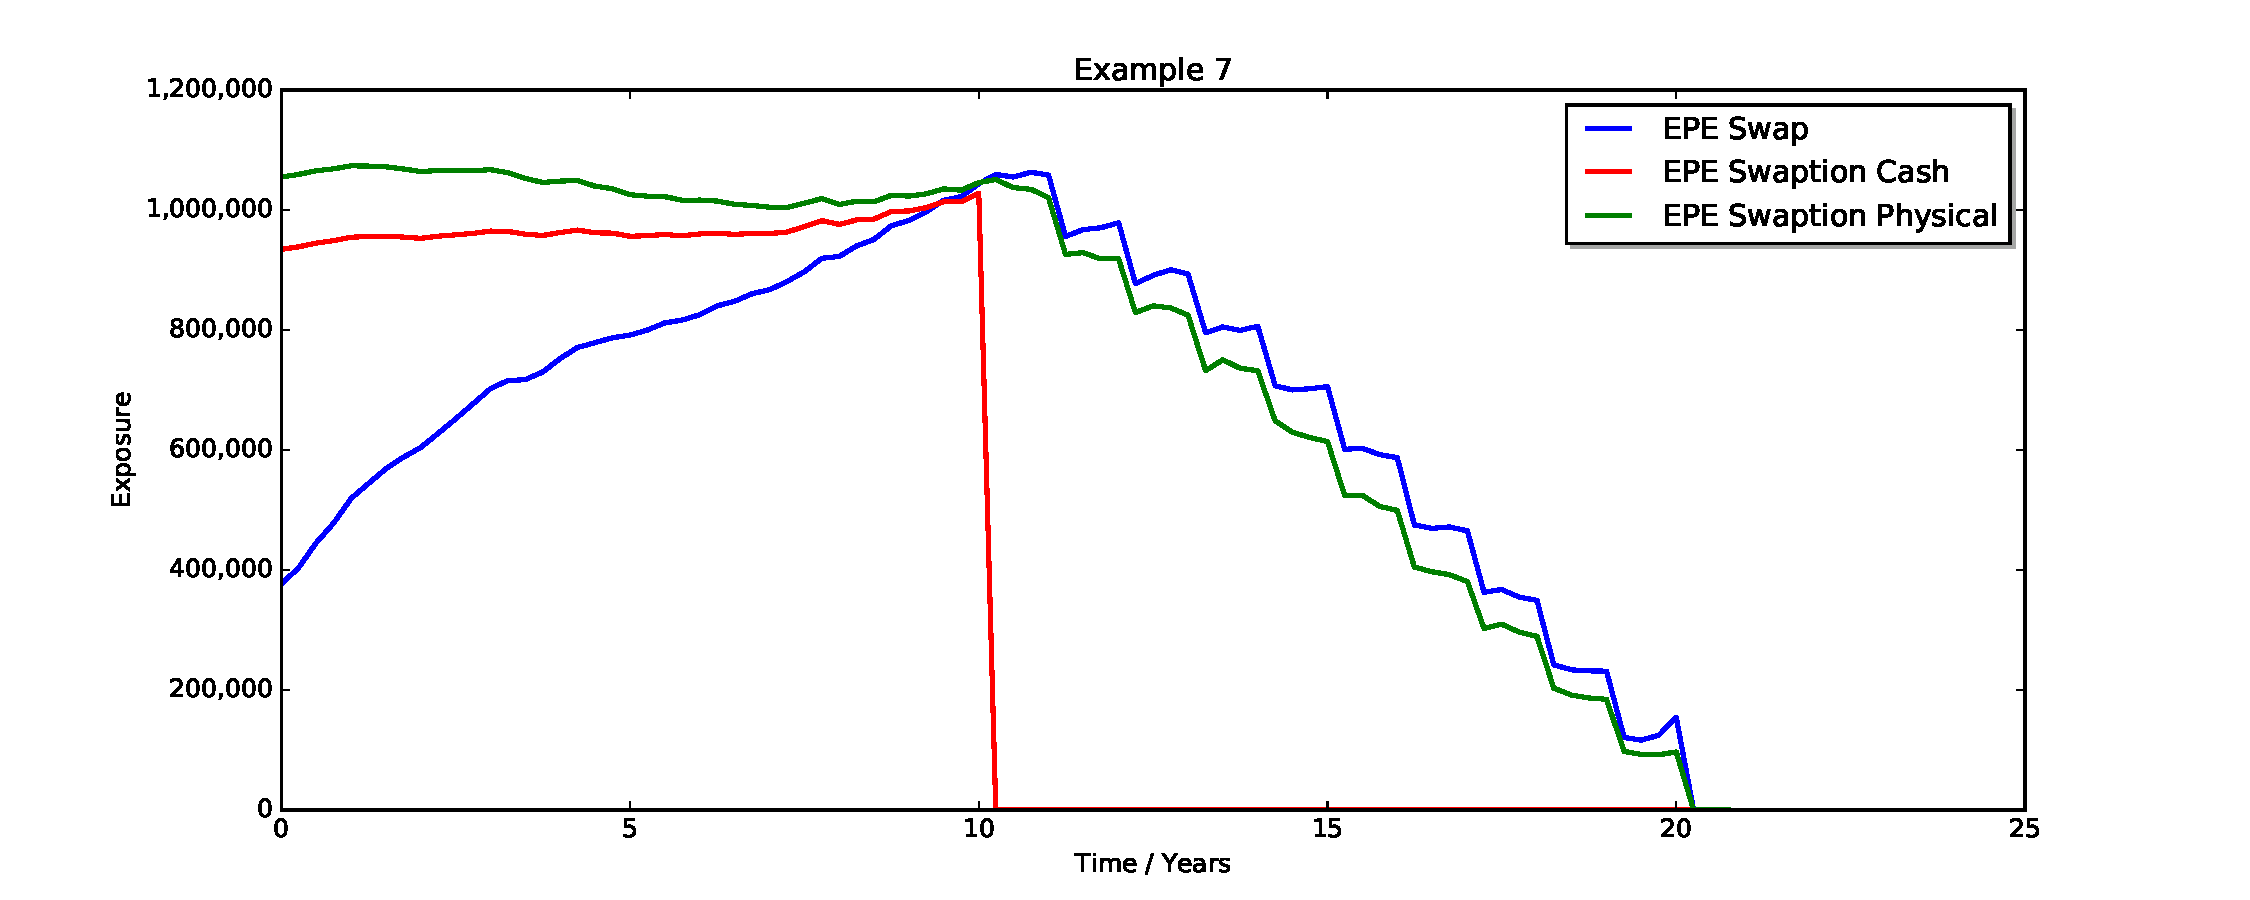
\includegraphics[scale=0.45]{mpl_swaption.pdf}
\end{center}
\caption{European Swaption exposure evolution, expiry in 10 years, final maturity in 20 years, for cash and physical
  delivery. Simulation with 1000 paths and quarterly time steps. }
\label{fig_3}
\end{figure}
The delivery type (cash vs physical) yields significantly different valuations as of today due to the steepness of the
relevant yield curves (EUR). The cash settled Swaption's exposure graph is truncated at the exercise date, whereas the
physically settled Swaption exposure turns into a Swap-like exposure after expiry. For comparison, the example also
provides the exposure evolution of the underlying forward starting Swap which yields a somewhat higher exposure after
the forward start date than the physically settled Swaption. This is due to scenarios with negative Swap NPV at expiry
(hence not exercised) and positive NPVs thereafter. Note the reduced EPE in case of a Swaption with settlement of the option premium on exercise date.

%--------------------------------------------------------
\subsection{Bermudan Swaption Exposure}
%--------------------------------------------------------

This demo case in folder {\tt Examples/Example\_4} shows the exposure evolution of Bermudan rather than European
Swaptions with cash and physical delivery, respectively, see figure \ref{fig_3b}.
\begin{figure}[h!]
\begin{center}
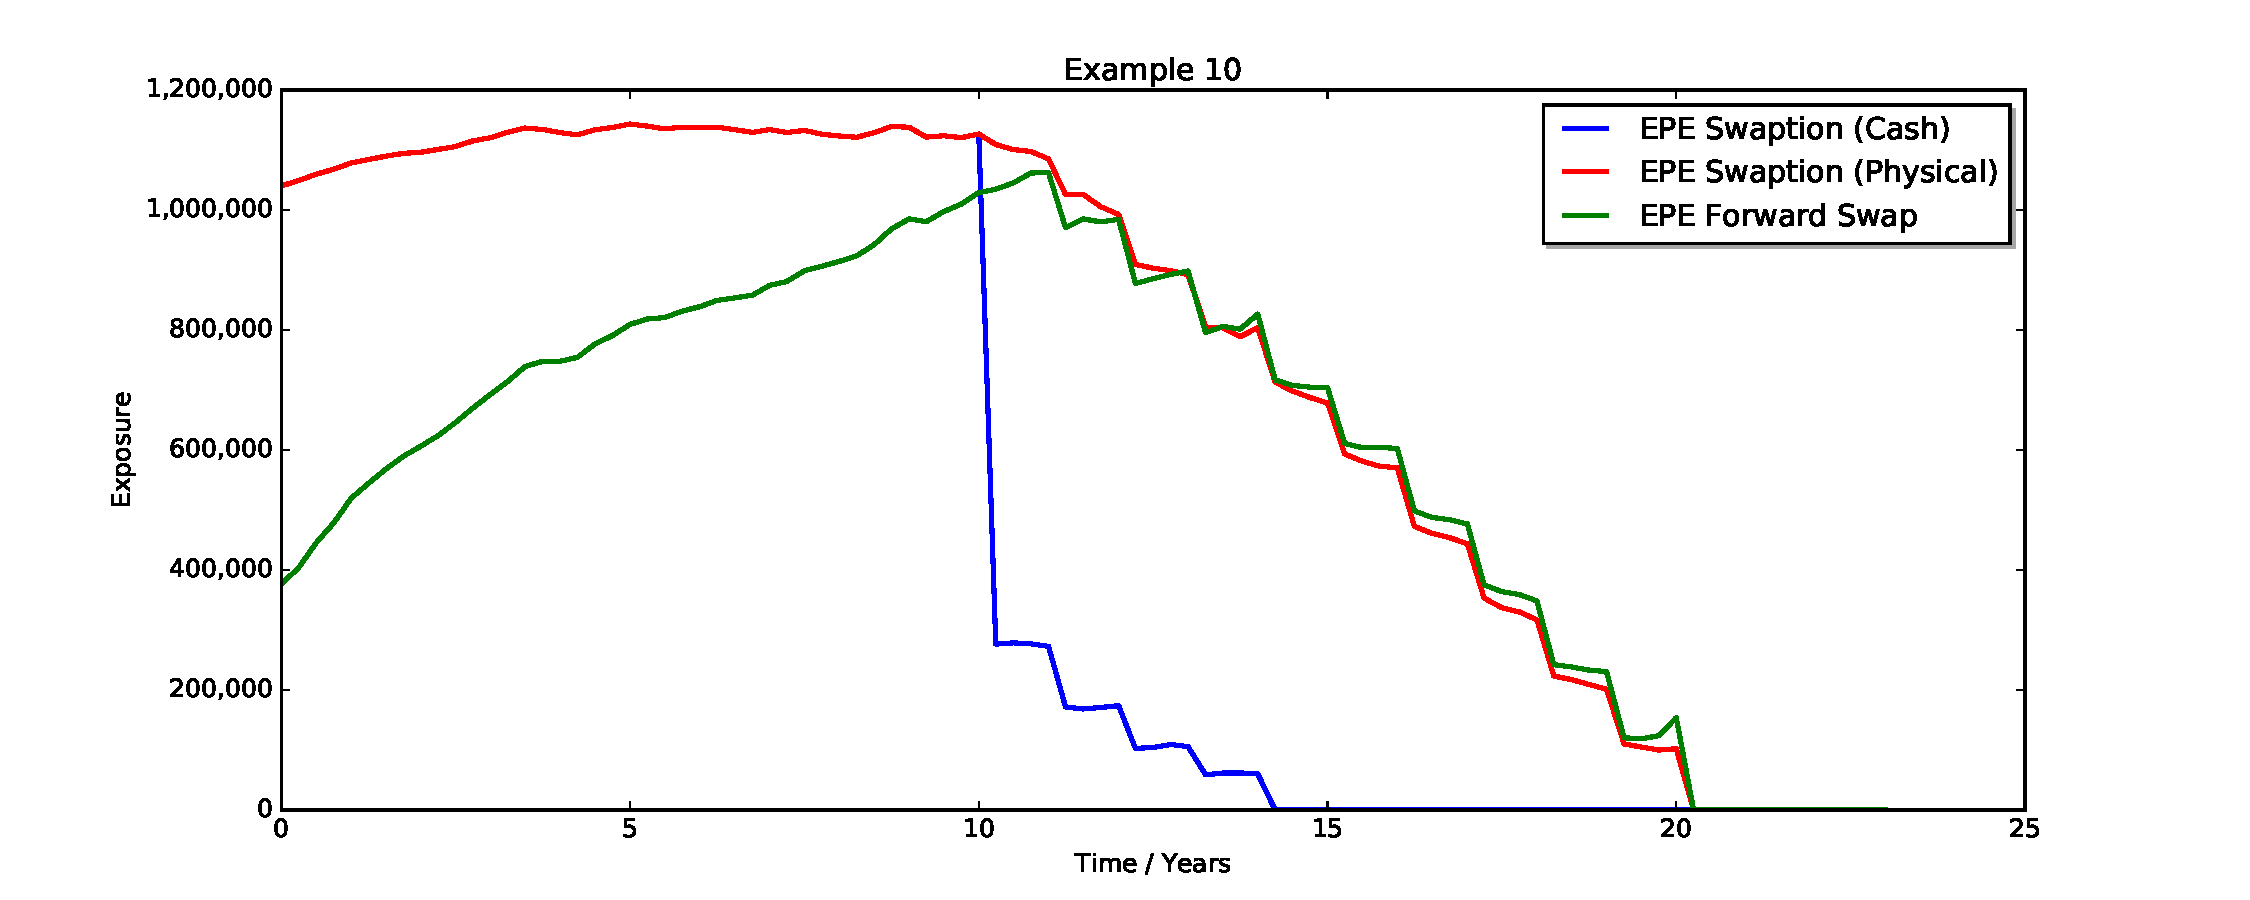
\includegraphics[scale=0.45]{mpl_bermudan_swaption.pdf}
\end{center}
\caption{Bermudan Swaption exposure evolution, 5 annual exercise dates starting in 10 years, final maturity in 20 years,
  for cash and physical delivery. Simulation with 1000 paths and quarterly time steps.}
\label{fig_3b}
\end{figure}
The underlying Swap is the same as in the European Swaption example in section \ref{sec:european_swaption}. Note in
particular the difference between the Bermudan and European Swaption exposures with cash settlement: The Bermudan shows
the typical step-wise decrease due to the series of exercise dates. Also note that we are using the same Bermudan option
pricing engines for both settlement types, in contrast to the European case, so that the Bermudan option cash and
physical exposures are identical up to the first exercise date. When running this example, you will notice the
significant difference in computation time compared to the European case (ballpark 30 minutes here for 2 Swaptions, 1000
samples, 90 time steps). The Bermudan example takes significantly more computation time because we use an LGM grid
engine for pricing under scenarios in this case. In a realistic context one would more likely resort to American Monte
Carlo simulation, feasible in ORE, but not provided in the current release. However, this implementation can be used to
benchmark any faster / more sophisticated approach to Bermudan Swaption exposure simulation.

%--------------------------------------------------------
\subsection{Callable Swap Exposure}
%--------------------------------------------------------

This demo case in folder {\tt Examples/Example\_5} shows the exposure evolution of a European callable Swap, represented
as two trades - the non-callable Swap and a Swaption with physical delivery. We have sold the call option, i.e. the
Swaption is a right for the counterparty to enter into an offsetting Swap which economically terminates all future flows
if exercised. The resulting exposure evolutions for the individual components (Swap, Swaption), as well as the callable
Swap are shown in figure \ref{fig_4}.
\begin{figure}[h!]
\begin{center}
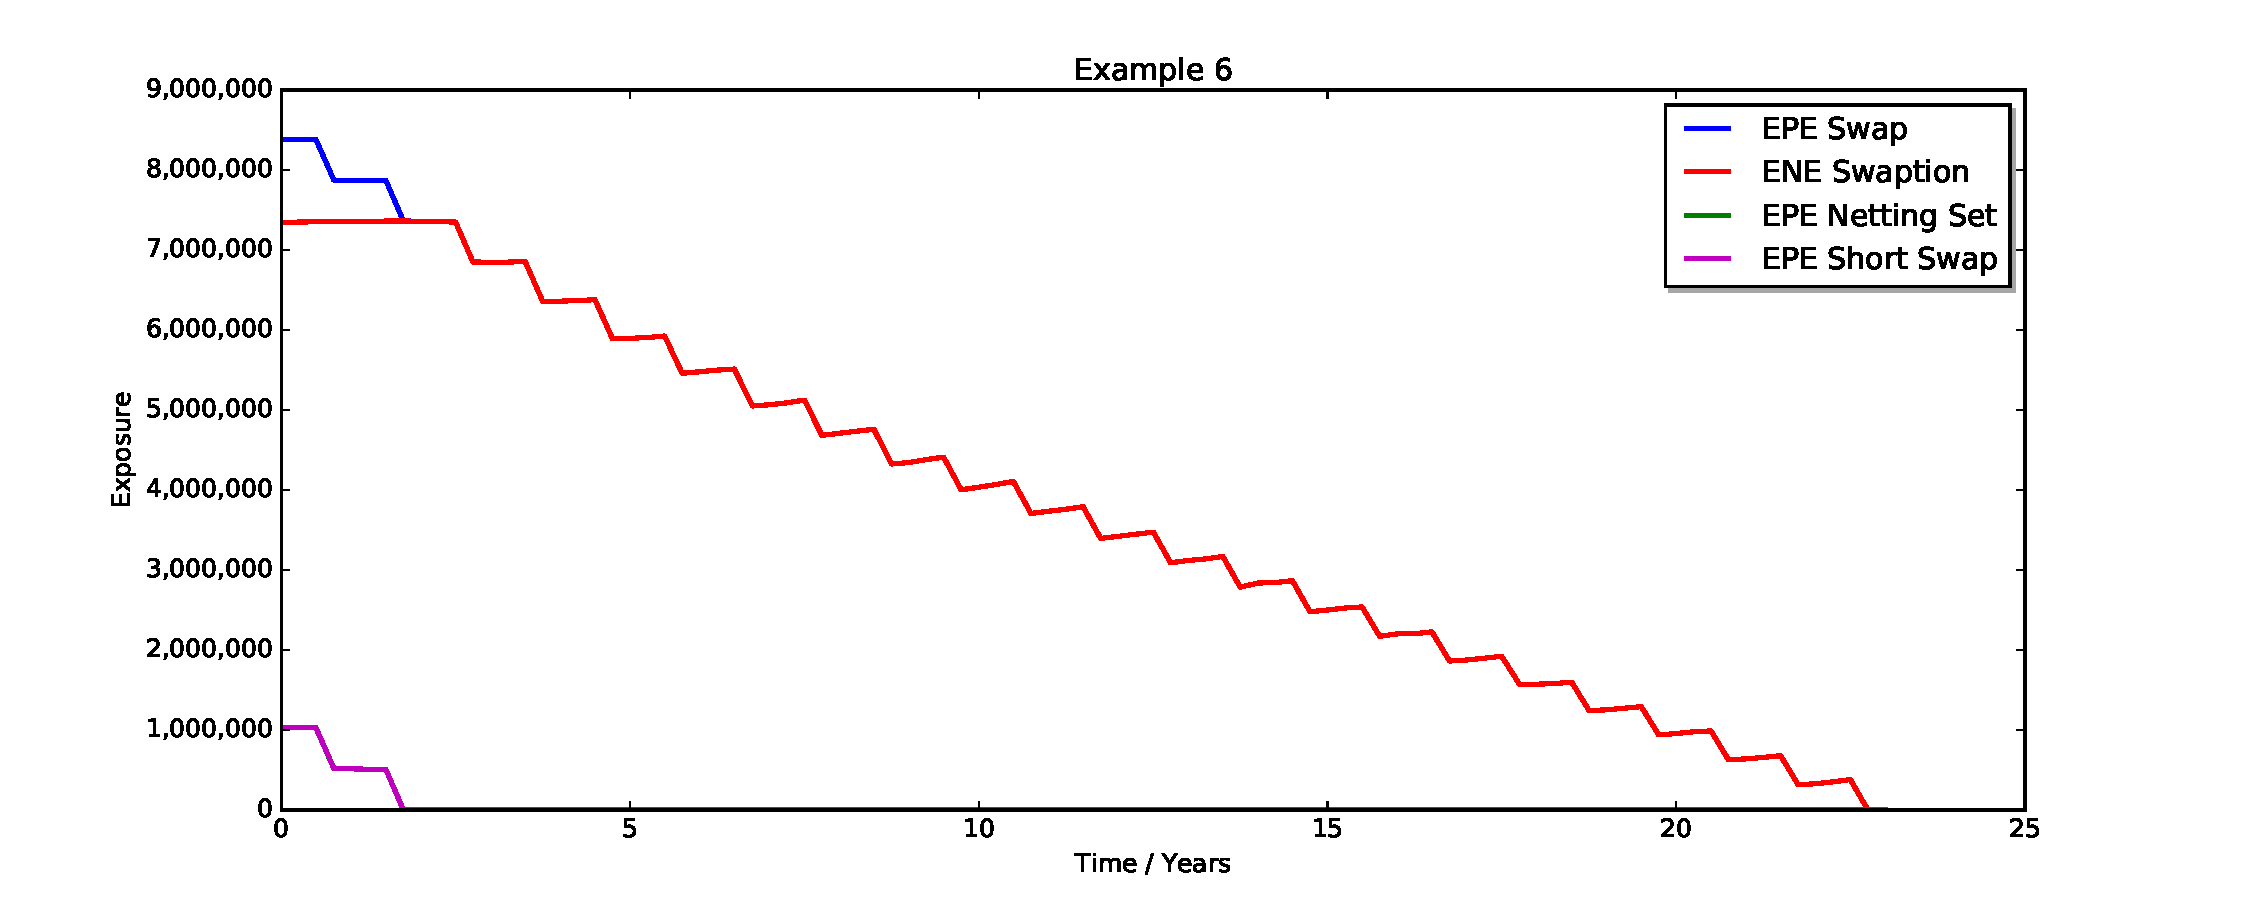
\includegraphics[scale=0.45]{mpl_callable_swap.pdf}
\end{center}
\caption{European callable Swap represented as a package consisiting of non-callable Swap and Swaption. The Swaption has
  physical delivery and offsets all future Swap cash flows if exercised. The exposure evolution of the package is shown
  here as 'EPE Netting Set' (green line). This is covered by the pink line, the exposure evolution of the same Swap but
  with maturity on the exercise date. The graphs match perfectly here, because the example Swap is deep in the money and
  exercise probability is close to one. Simulation with 5000 paths and quarterly time steps.}
\label{fig_4}
\end{figure}
The example is an extreme case where the underlying Swap is deeply in the money (receiving fixed 5\%), and hence the
call exercise probability is close to one. Modify the Swap and Swaption fixed rates closer to the money ($\approx$ 1\%)
to see the deviation between net exposure of the callable Swap and the exposure of a 'short' Swap with maturity on
exercise.

%--------------------------------------------------------
\subsection{Cap/Floor Exposure}\label{sec:capfloor}
%--------------------------------------------------------

The example in folder {\tt Examples/Example\_6} generates exposure evolutions of several Swaps, caps and floors. The
example shown in figure \ref{fig_capfloor_1} ('portfolio 1') consists of a 20y Swap receiving 3\% fixed and paying
Euribor 6M plus a long 20y Collar
with both cap and floor at 4\% so that the net exposure corresponds to a Swap paying 1\% fixed. \\

\begin{figure}[h!]
\begin{center}
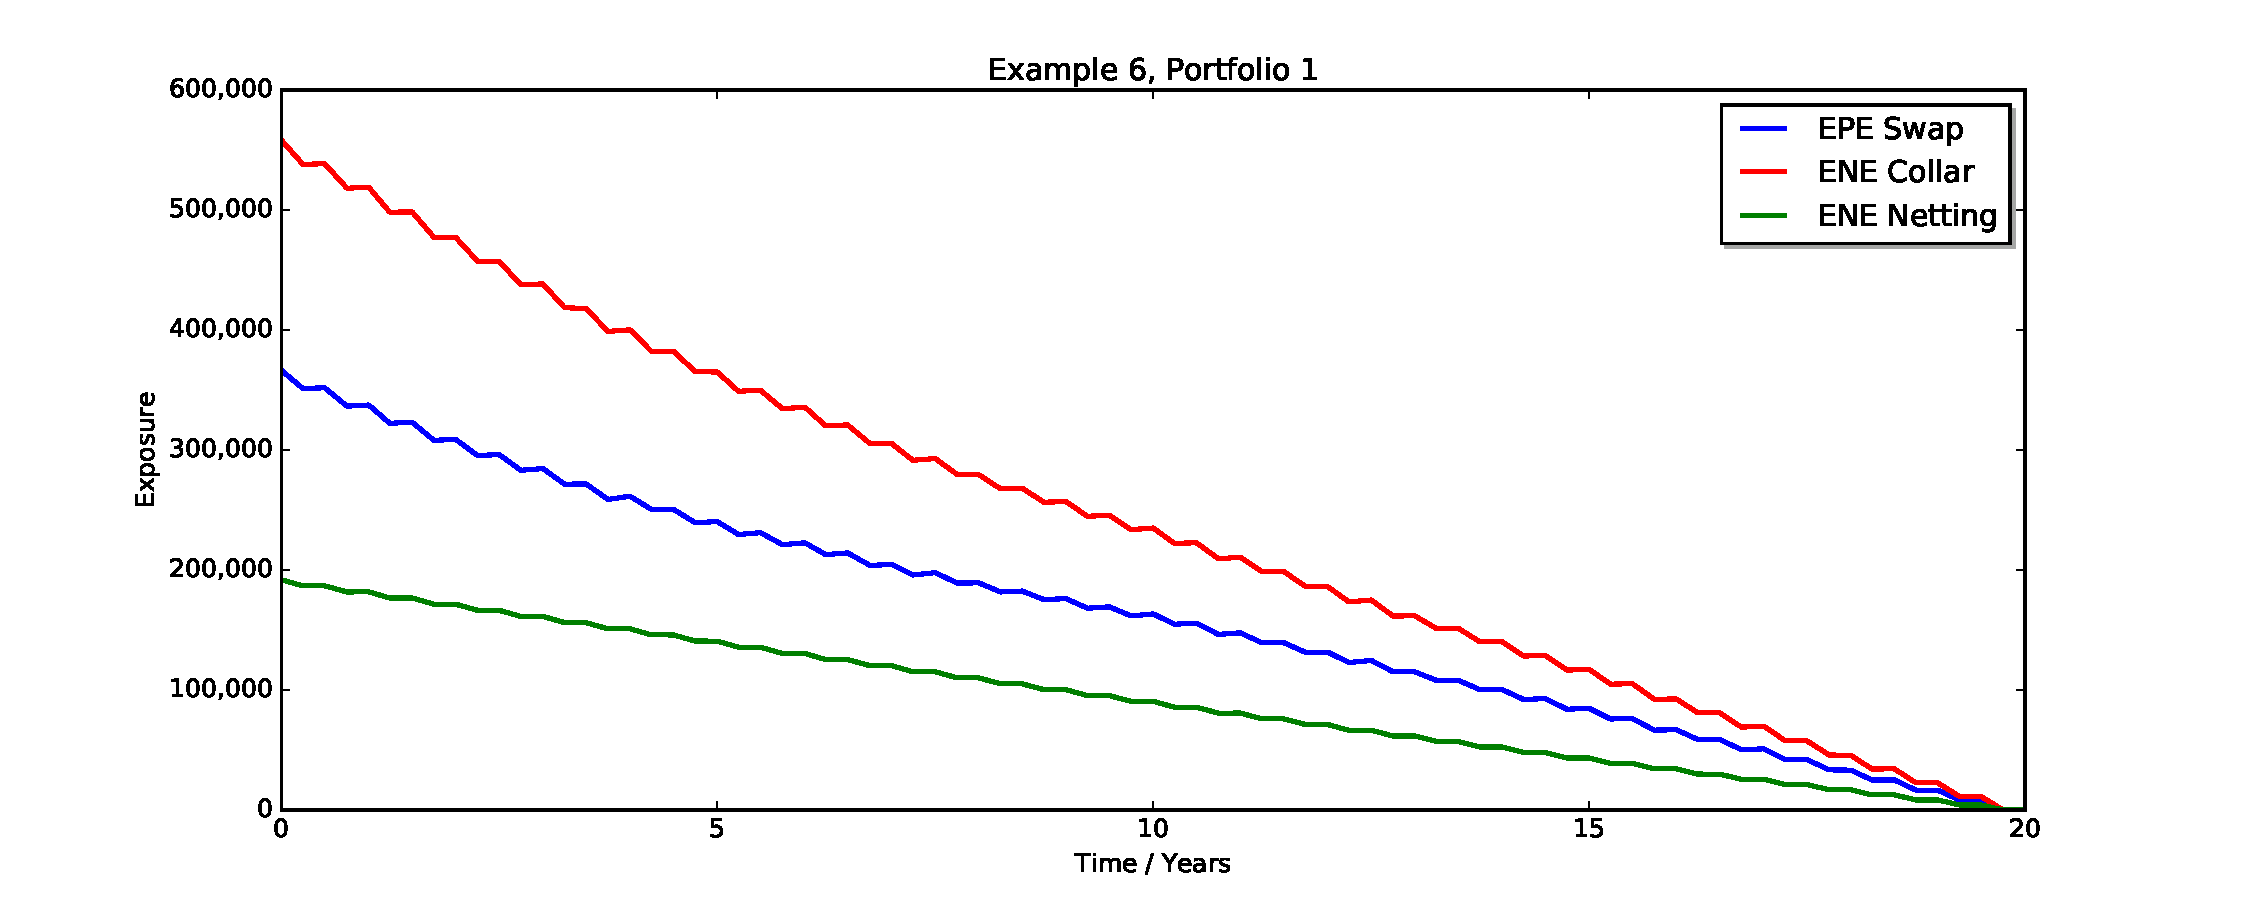
\includegraphics[scale=0.45]{mpl_capfloor_1.pdf}
\end{center}
\caption{Swap+Collar, portfolio 1. The Collar has identical cap and floor rates at 4\% so that it corresponds to a
  fixed leg which reduces the exposure of the Swap, which receives 3\% fixed. Simulation with 1000 paths and quarterly
  time steps.}
\label{fig_capfloor_1}
\end{figure}

The second example in this folder shown in figure \ref{fig_capfloor_2} ('portfolio 2') consists of a short Cap, long
Floor and a long Collar that exactly offsets the netted Cap and Floor.

\begin{figure}[h!]
\begin{center}
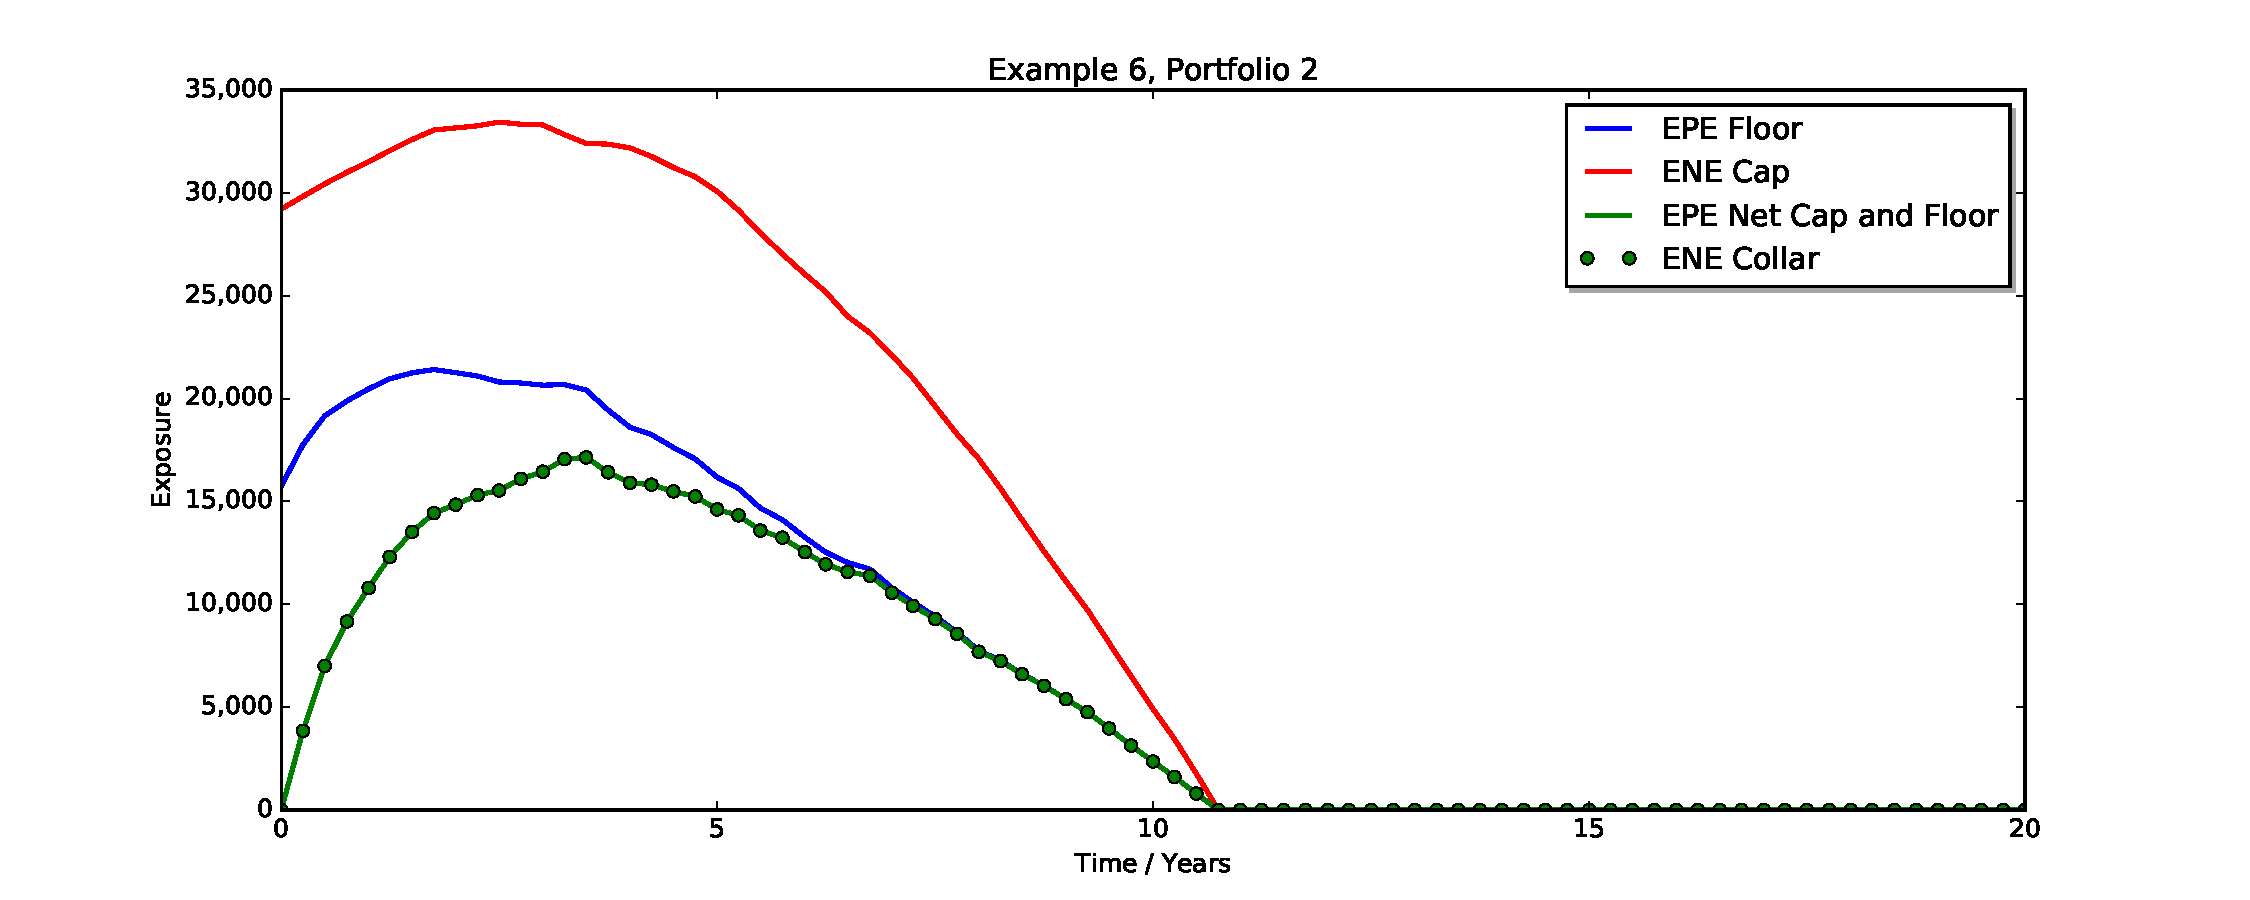
\includegraphics[scale=0.45]{mpl_capfloor_2.pdf}
\end{center}
\caption{Short Cap and long Floor vs long Collar, portfolio 2. Simulation with 1000 paths and quarterly time steps.}
\label{fig_capfloor_2}
\end{figure}

Further three test portfolios are provided as part of this example. Run the example and inspect the respective output
directories {\tt Examples/Example\_6/Output/portfolio\_\#}. Note that these directories have to be present/created
before running the batch with {\tt python run.py}.

%--------------------------------------------------------
\subsection{FX Forward and FX Option Exposure}\label{sec:fxfwd}
%--------------------------------------------------------

The example in folder {\tt Examples/Example\_7} generates the exposure evolution for a EUR / USD FX Forward transaction
with value date in 10Y. This is a particularly simple show case because of the single cash flow in 10Y. On the other
hand it checks the cross currency model implementation by means of comparison to analytic limits - EPE and ENE at the
trade's value date must match corresponding Vanilla FX Option prices, as shown in figure \ref{fig_5}.
\begin{figure}[h]
\begin{center}
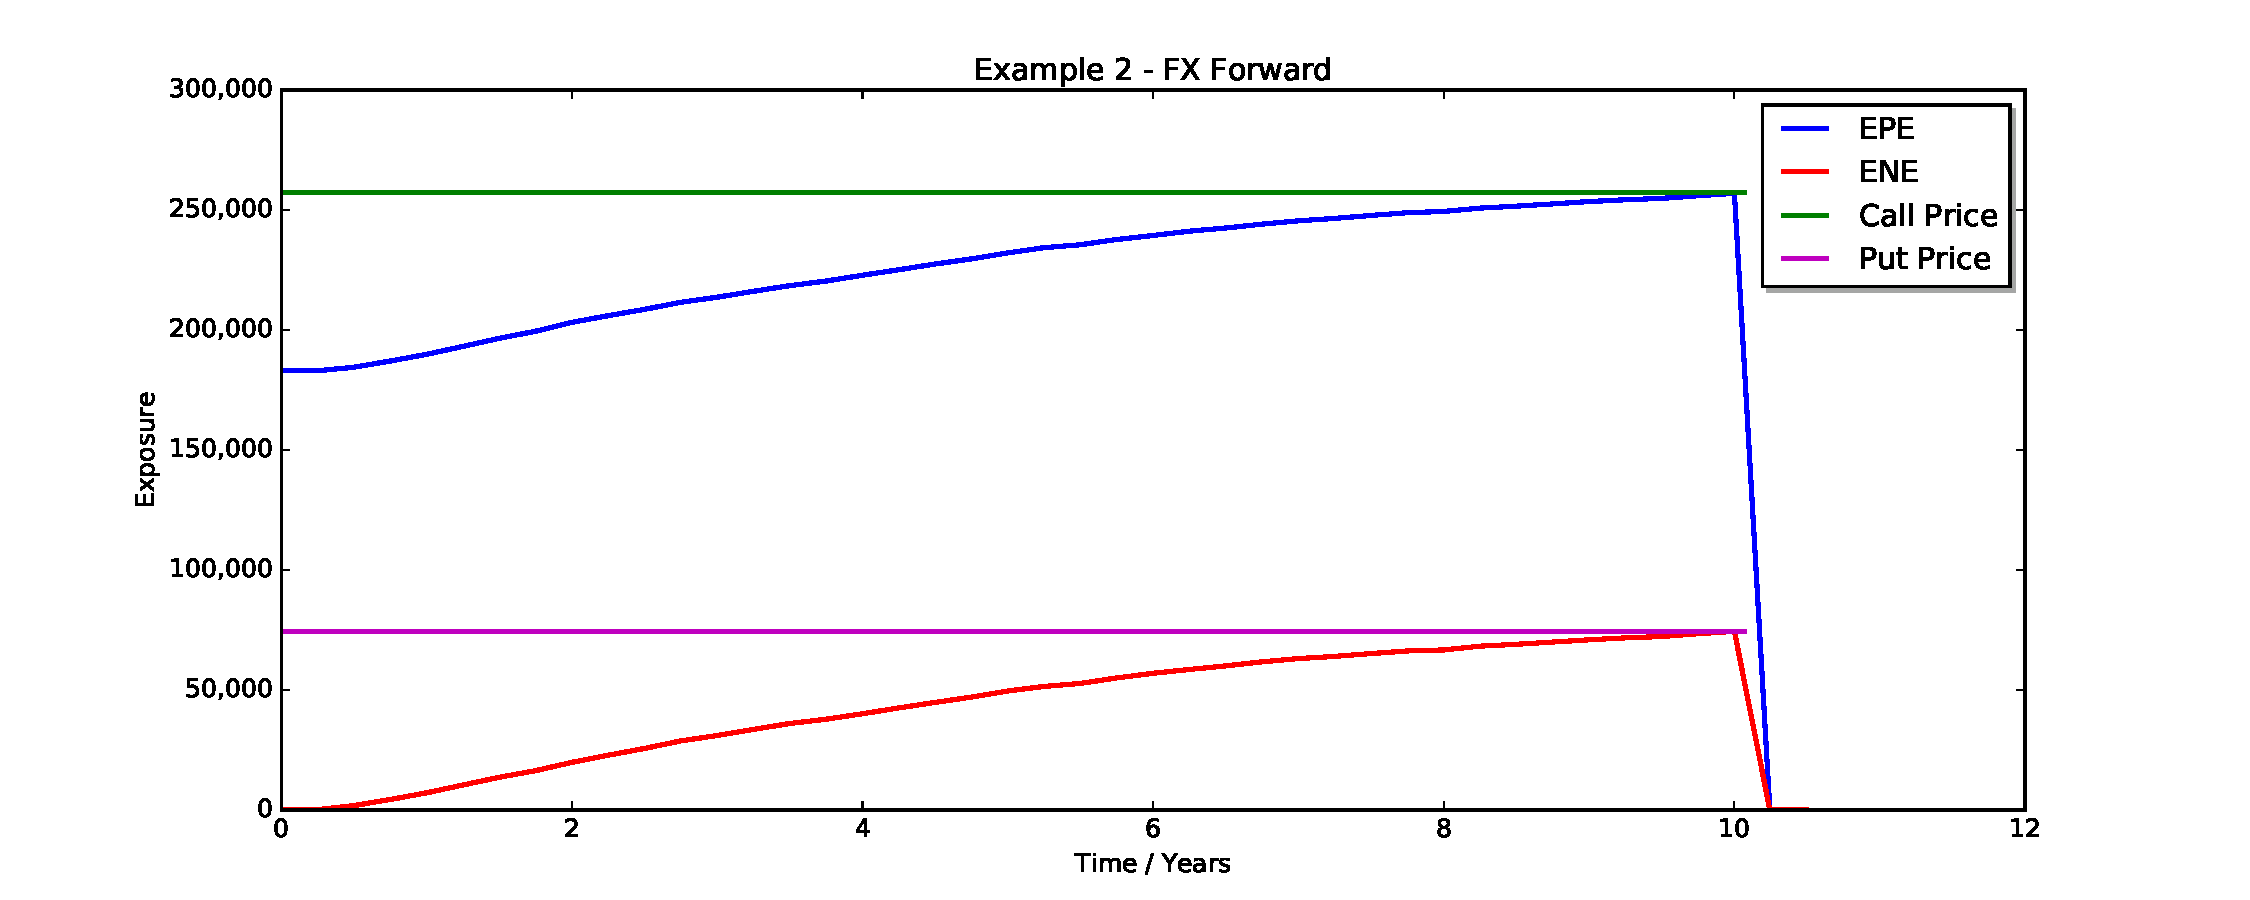
\includegraphics[scale=0.45]{mpl_fxforward.pdf}
\end{center}
\caption{EUR/USD FX Forward expected exposure in a realistic market environment as of 26/02/2016 from both parties'
  perspectives. Value date is obviously in 10Y. The flat lines are FX Option prices which coincide with EPE and ENE,
  respectively, on the value date. Simulation with 5000 paths and quarterly time steps.}
\label{fig_5}
\end{figure}

%--------------------------------------------------------
\subsection*{FX Option Exposure}\label{sec:fxoption}
%--------------------------------------------------------

This example (in folder {\tt Examples/Example\_7}, as the FX Forward example) illustrates the exposure evolution for an
FX Option, see figure \ref{fig_7}.
\begin{figure}[h!]
\begin{center}
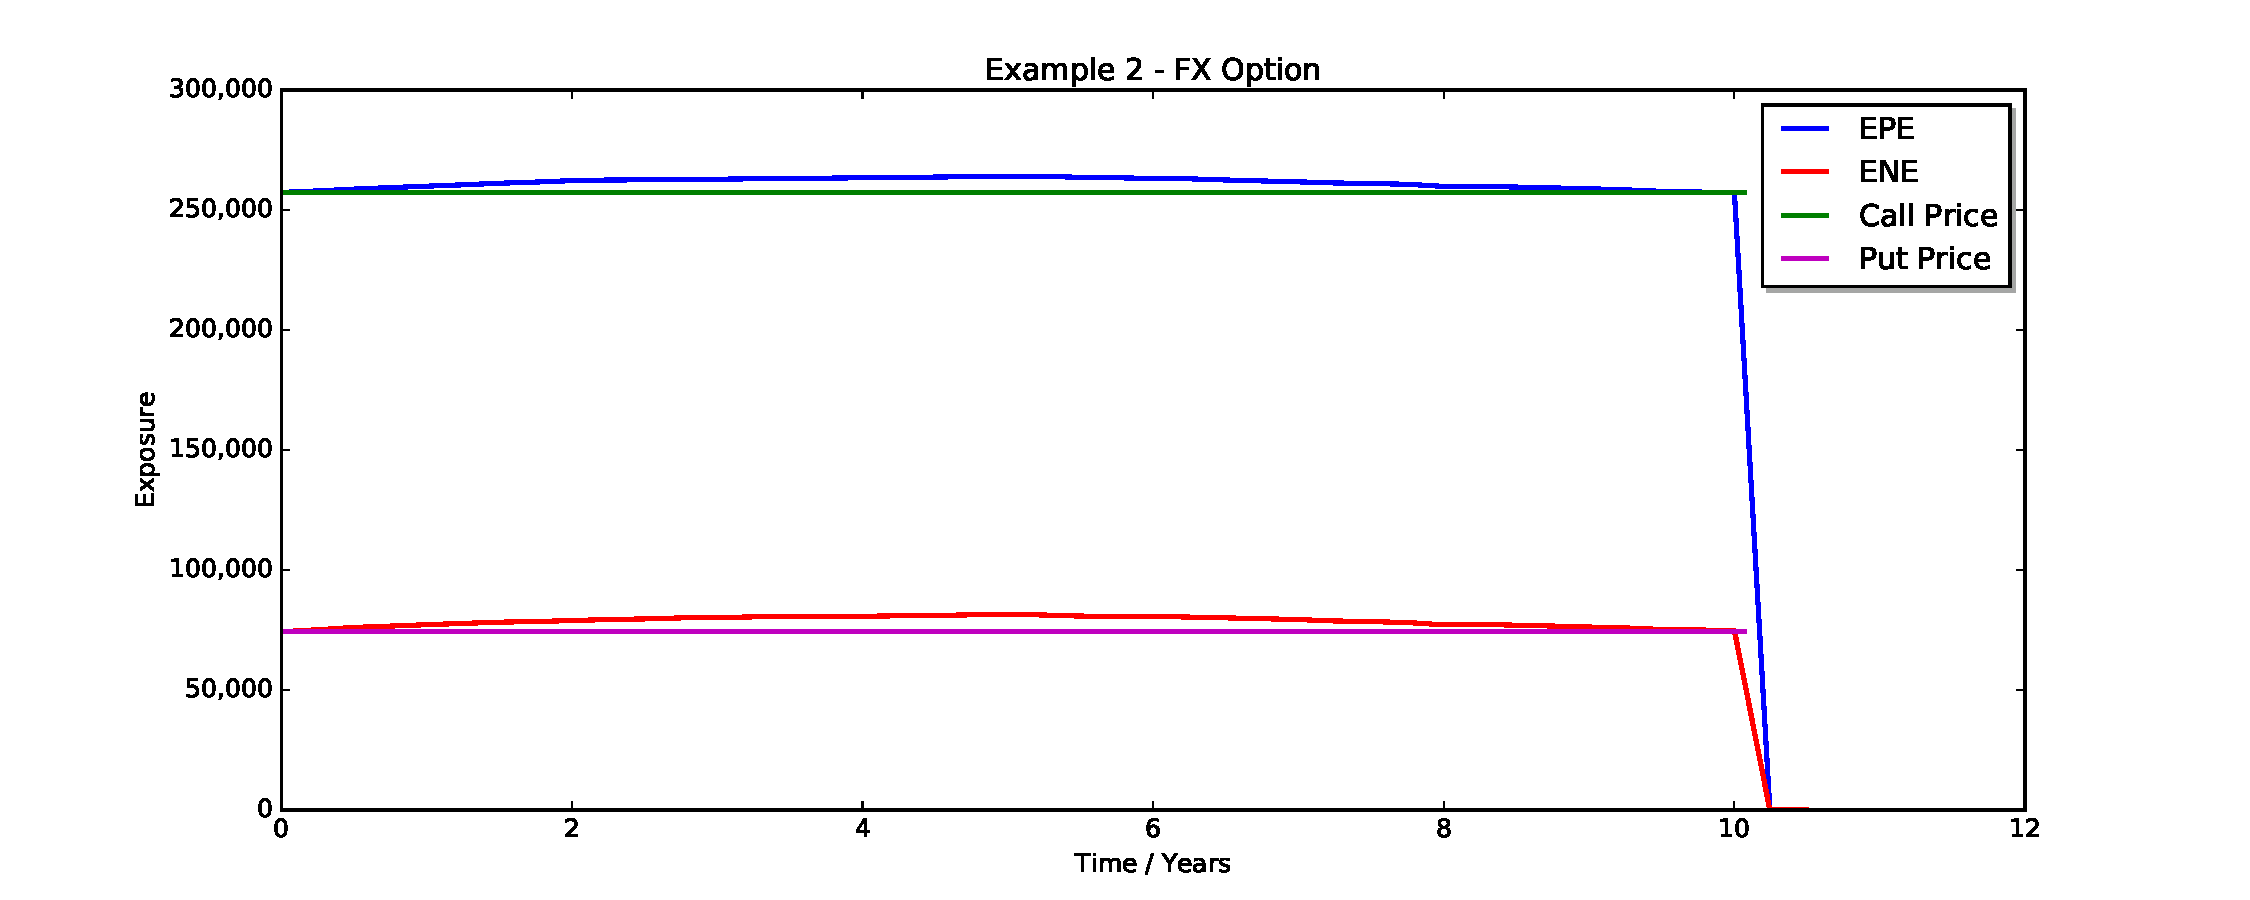
\includegraphics[scale=0.45]{mpl_fxoption.pdf}
\end{center}
\caption{EUR/USD FX Call and Put Option exposure evolution, same underlying and market data as in section
  \ref{sec:fxfwd}, compared to the call and put option price as of today (flat line). Simulation with 5000 paths and
  quarterly time steps.}
\label{fig_7}
\end{figure}
Recall that the FX Option value $NPV(t)$ as of time $0 \leq t \leq T$ satisfies
\begin{align*}
\frac{NPV(t)}{N(t)} &= \mbox{Nominal}\times\E_t\left[\frac{(X(T) - K)^+}{N(T)}\right]\\
NPV(0) &= \E\left[\frac{NPV(t)}{N(t)}\right] = \E\left[\frac{NPV^+(t)}{N(t)} \right]= \EPE(t) 
\end{align*}
where $N(t)$ denotes the numeraire asset.
One would therefore expect a flat exposure evolution up to option expiry. The deviation from this in ORE's simulation is
due to the pricing approach chosen here under scenarios. A Black FX option pricer is used with deterministic Black
volatility derived from today's volatility structure (pushed or rolled forward, see section \ref{sec:sim_market}). The
deviation can be removed by extending the volatility modelling, e.g. implying model consistent Black volatilities in
each simulation step on each path.  
%\todo[inline]{Add exposure evolution graph with 'simulated' FX vol}

%--------------------------------------------------------
\subsection{Cross Currency Swap Exposure, without FX Reset}
%--------------------------------------------------------

The case in {\tt Examples/Example\_8} is a vanilla cross currency Swap. It shows the typical blend of an Interest Rate
Swap's saw tooth exposure evolution with an FX Forward's exposure which increases monotonically to final maturity, see
figure \ref{fig_6}.
\begin{figure}[h!]
\begin{center}
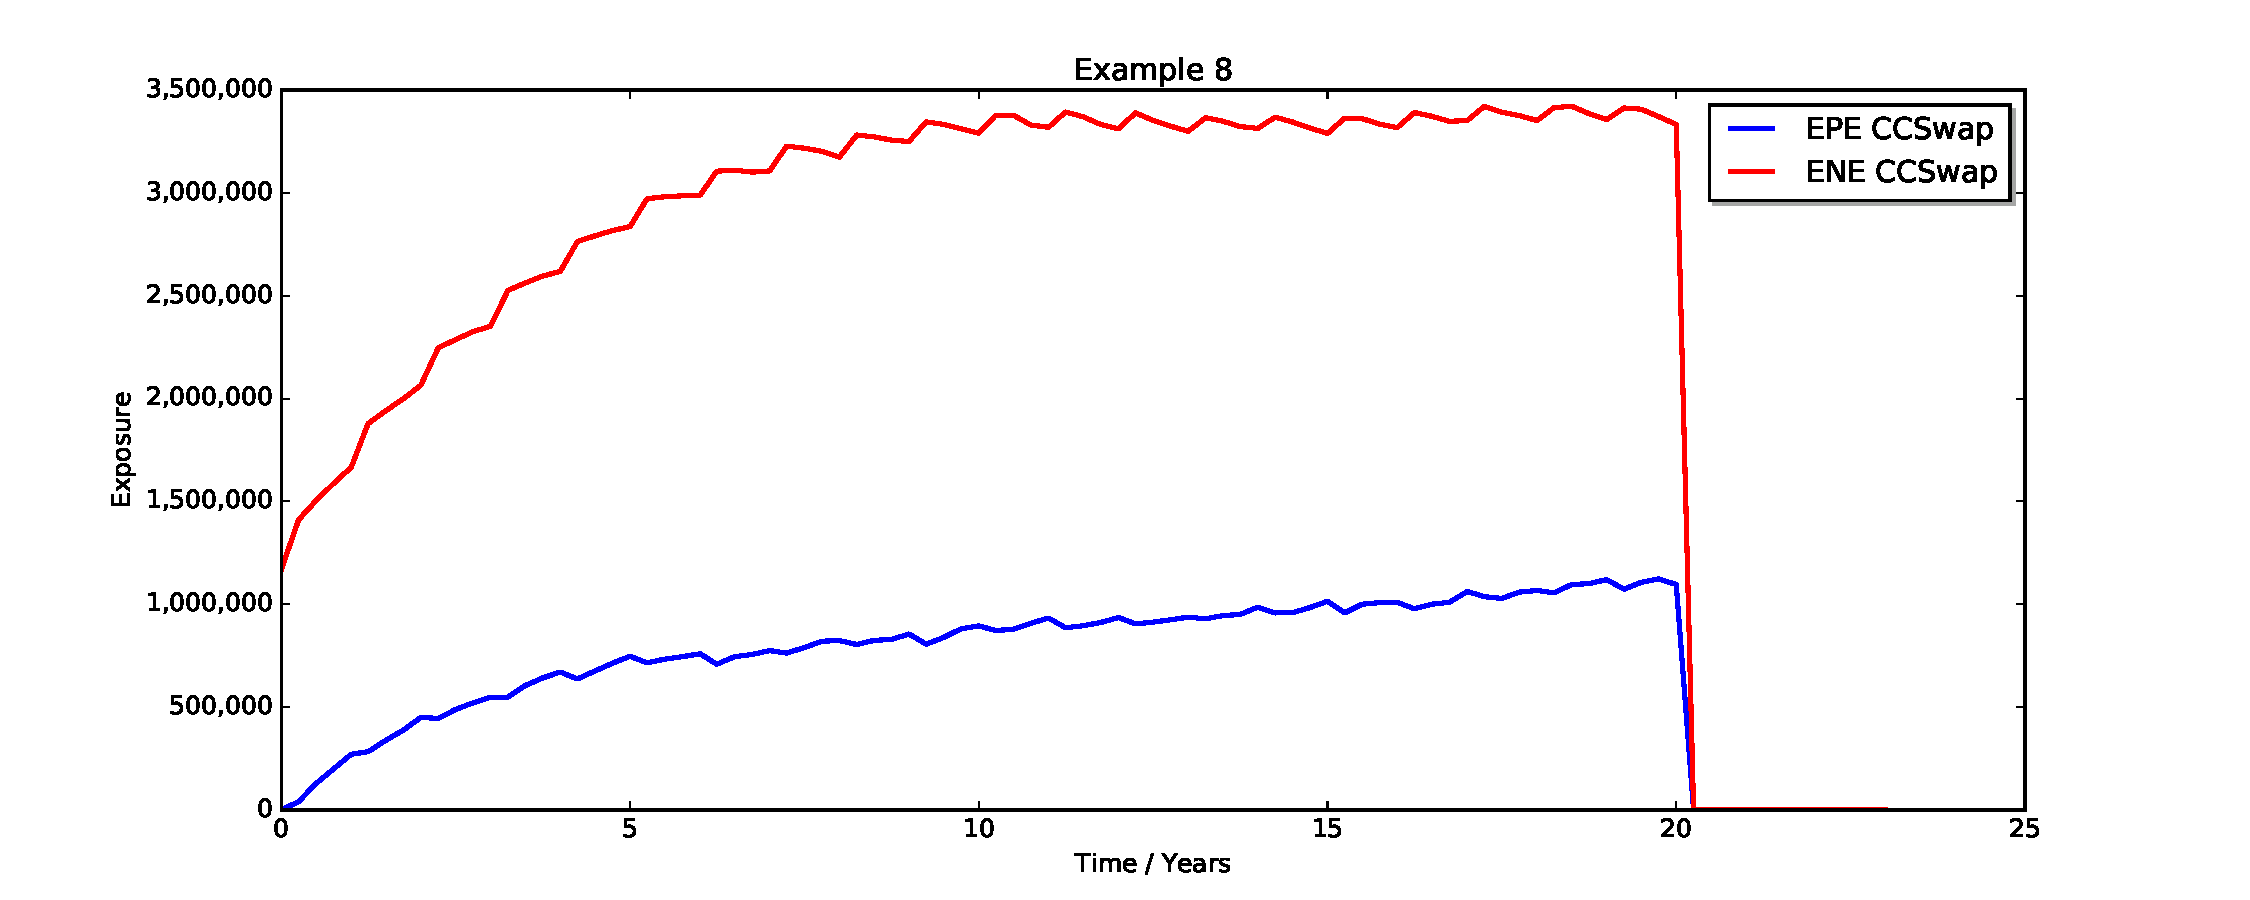
\includegraphics[scale=0.45]{mpl_ccswap.pdf}
\end{center}
\caption{Cross Currency Swap exposure evolution without mark-to-market notional reset. Simulation with 1000 paths and
  quarterly time steps.}
\label{fig_6}
\end{figure}

%--------------------------------------------------------
\subsection{Cross Currency Swap Exposure, with FX Reset}
%--------------------------------------------------------

The effect of the FX resetting feature, common in Cross Currency Swaps nowadays, is shown in {\tt Examples/Example\_9}.
The example shows the exposure evolution of a EUR/USD cross currency basis Swap with FX reset at each interest period
start, see figure \ref{fig_6b}. As expected, the notional reset causes an exposure collapse at each period start when
the EUR leg's notional is reset to match the USD notional.
\begin{figure}[h!]
\begin{center}
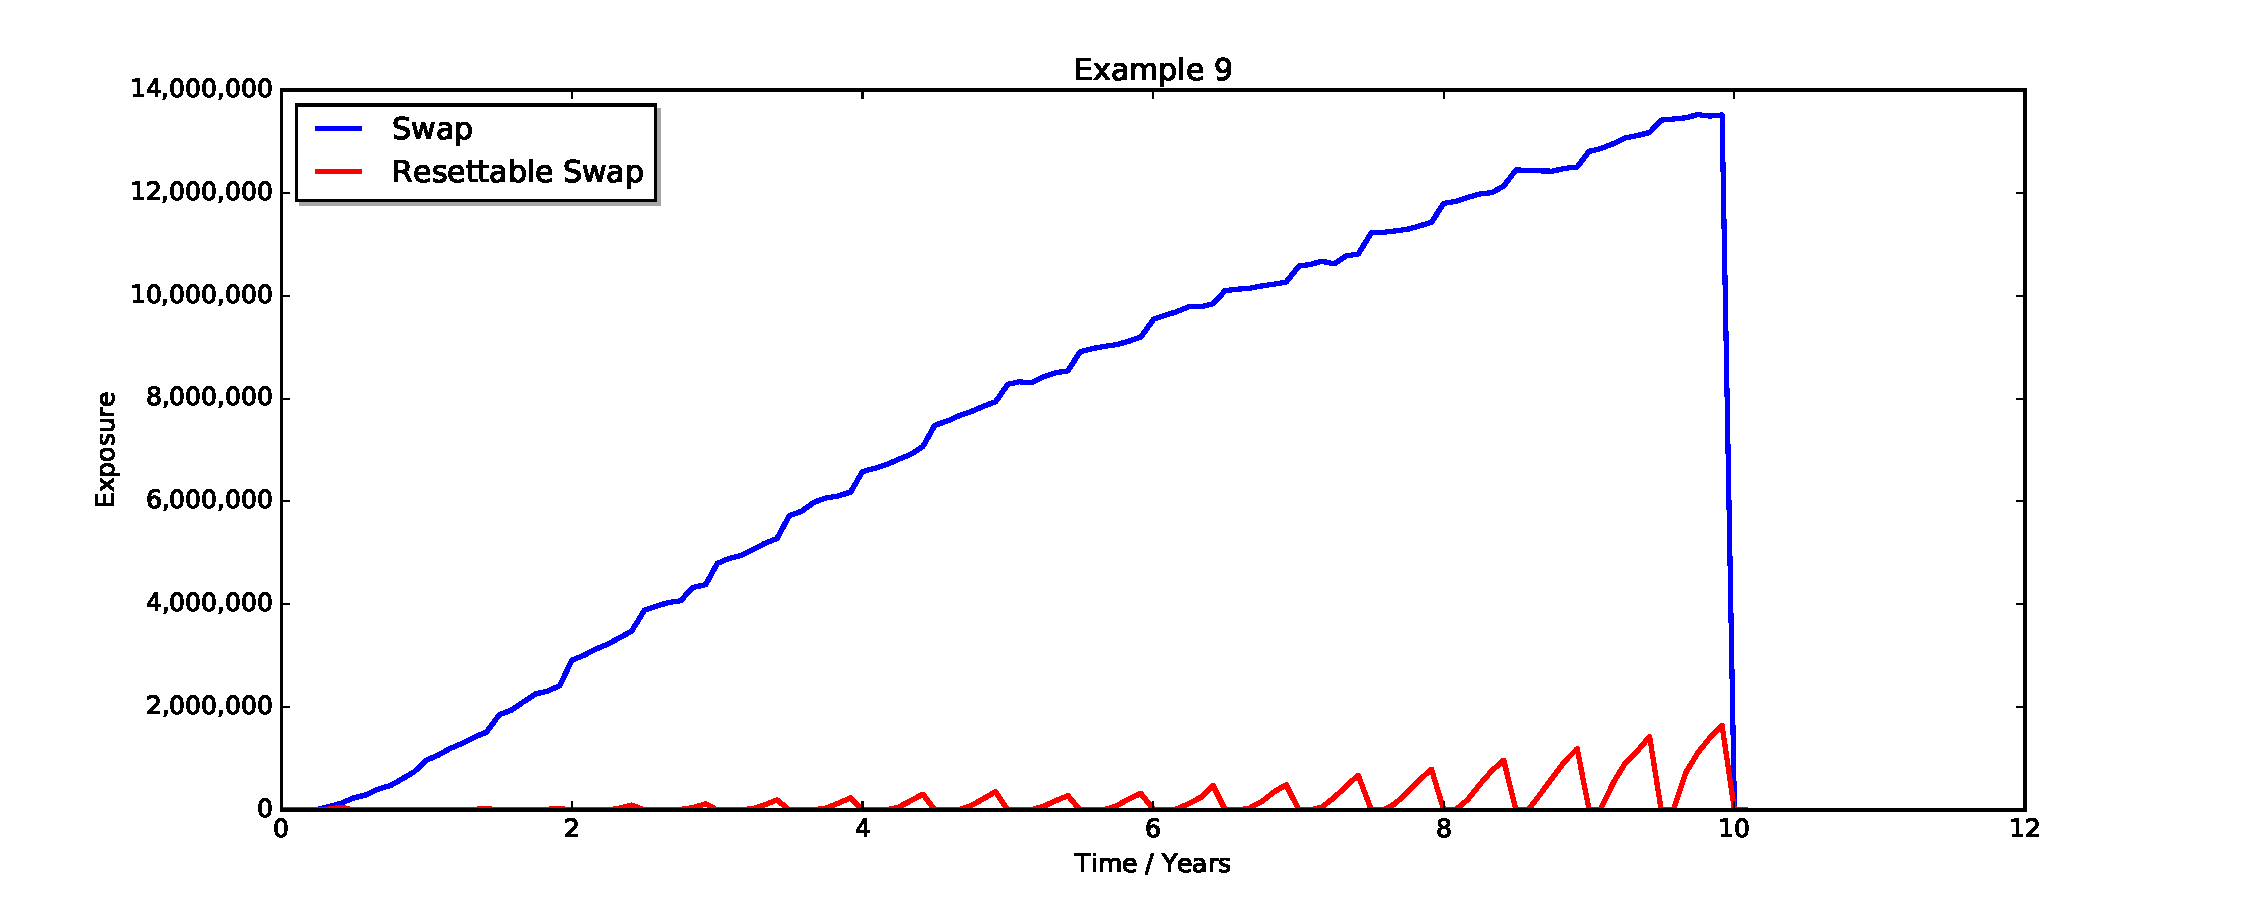
\includegraphics[scale=0.45]{mpl_xccy_reset.pdf}
\end{center}
\caption{Cross Currency Basis Swap exposure evolution with and without mark-to-market notional reset. Simulation with
  1000 paths and quarterly time steps.}
\label{fig_6b}
\end{figure}
  
%--------------------------------------------------------
\subsection{Netting Set, Collateral, XVAs, XVA Allocation}
%--------------------------------------------------------

In this example (see folder {\tt Examples/Example\_10}) we showcase a small netting set consisting of three Swaps in
different currencies, with different collateral choices
\begin{itemize}
\item no collateral - figure \ref{fig_8},
\item collateral with threshold (THR) 1m EUR, minimum transfer amount (MTA) 100k EUR, margin period of risk (MPOR) 2
  weeks - figure \ref{fig_9}
\item collateral with zero THR and MTA, and MPOR 2w - figure \ref{fig_10}
\end{itemize}
The exposure graphs with collateral and positive margin period of risk show typical spikes. What is causing these? As
sketched in appendix \ref{sec:app_collateral}, ORE uses a {\em classical collateral model} that applies collateral
amounts to offset exposure with a time delay that corresponds to the margin period of risk. The spikes are then caused
by instrument cash flows falling between exposure measurement dates $d_1$ and $d_2$ (an MPOR apart), so that a
collateral delivery amount determined at $d_1$ but settled at $d_2$ differs significantly from the closeout amount at
$d_2$ causing a significant residual exposure for a short period of time. See for example \cite{Andersen2016} for a
recent detailed discussion of collateral modelling. The approach currently implemented in ORE corresponds to {\em
  Classical+} in \cite{Andersen2016}, the more conservative approach of the classical methods. The less conservative
alternative, {\em Classical-}, would assume that both parties stop paying trade flows at the beginning of the MPOR, so
that the P\&L over the MPOR does not contain the cash flow effect, and exposure spikes are avoided. Note that the size
and position of the largest spike in figure \ref{fig_9} is consistent with a cash flow of the 40 million GBP Swap in the
example's portfolio that rolls over the 3rd of March and has a cash flow on 3 March 2020, a bit more than four years
from the evaluation date.
  
\begin{figure}[h!]
\begin{center}
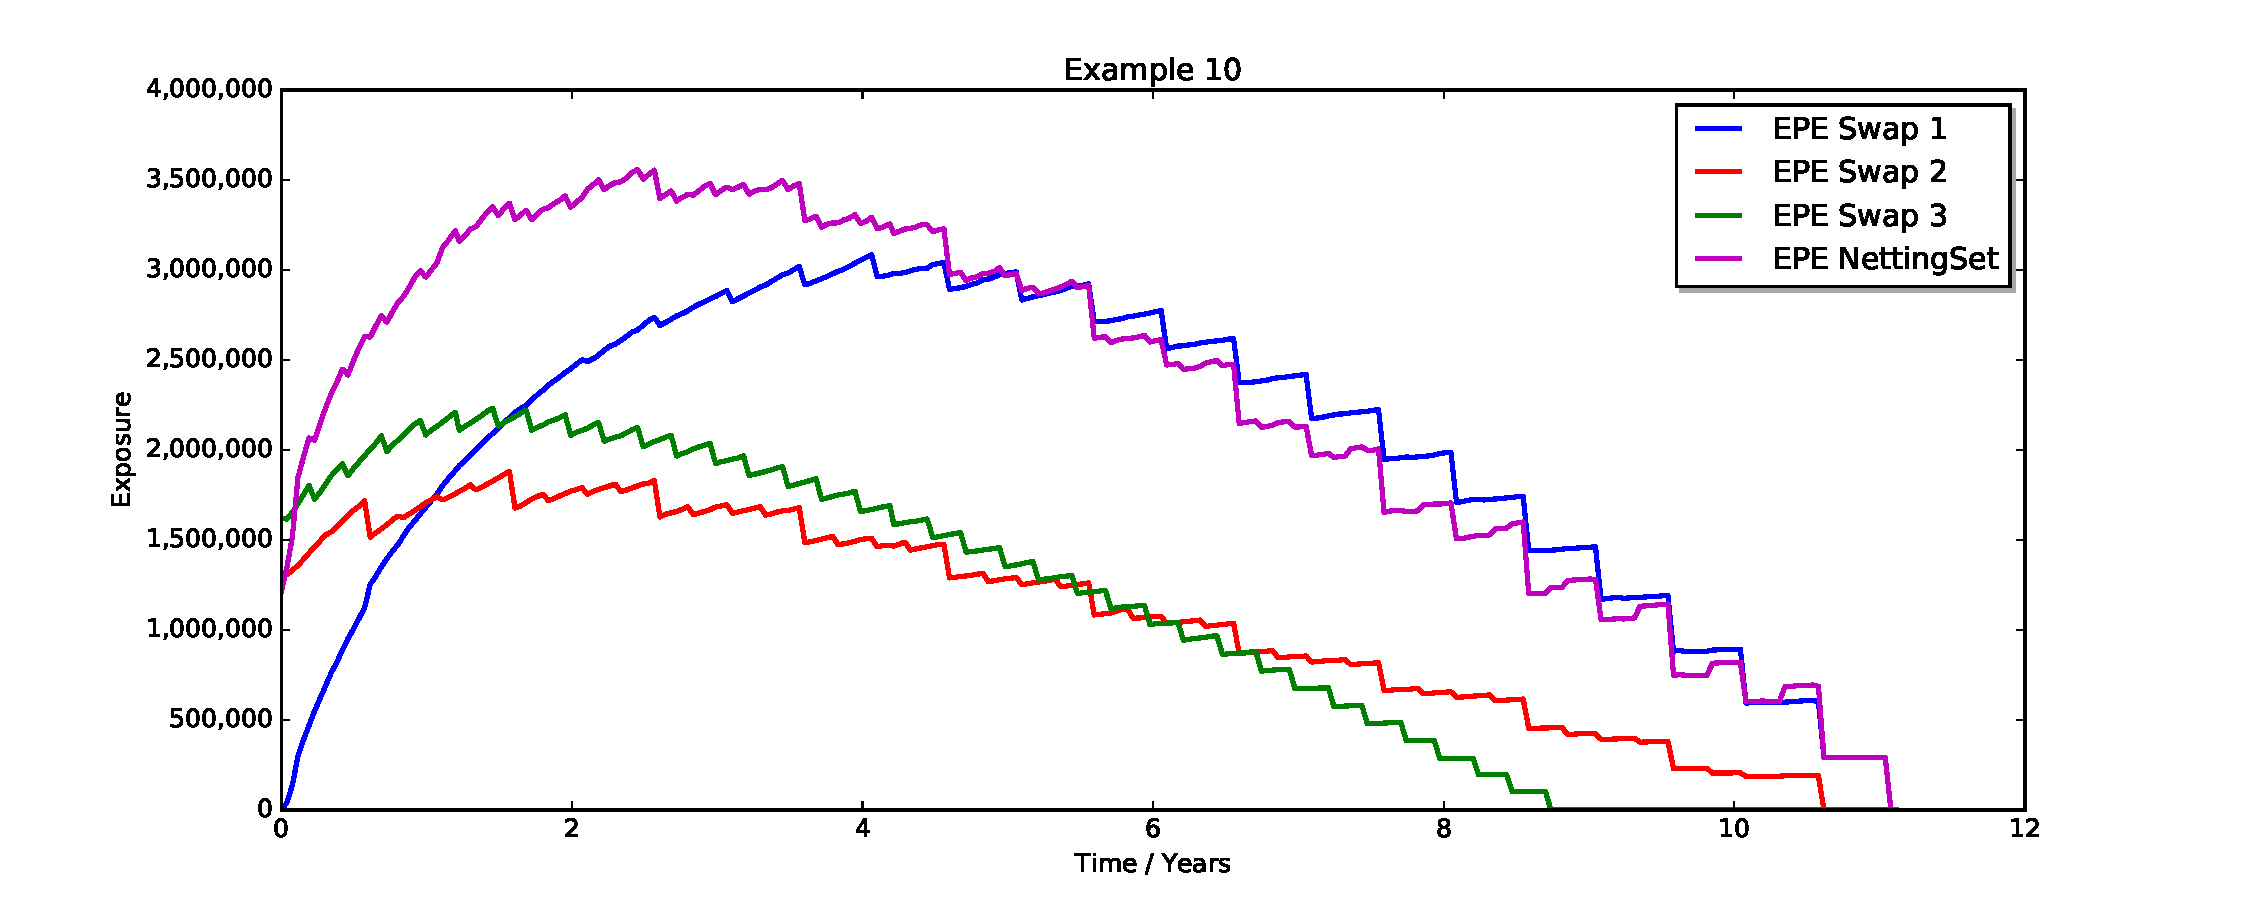
\includegraphics[scale=0.45]{mpl_nocollateral_epe.pdf}
\end{center}
\caption{Three Swaps netting set, no collateral. Simulation with 5000 paths and bi-weekly time steps.}
\label{fig_8}
\end{figure}

\begin{figure}[htb]
\begin{center}
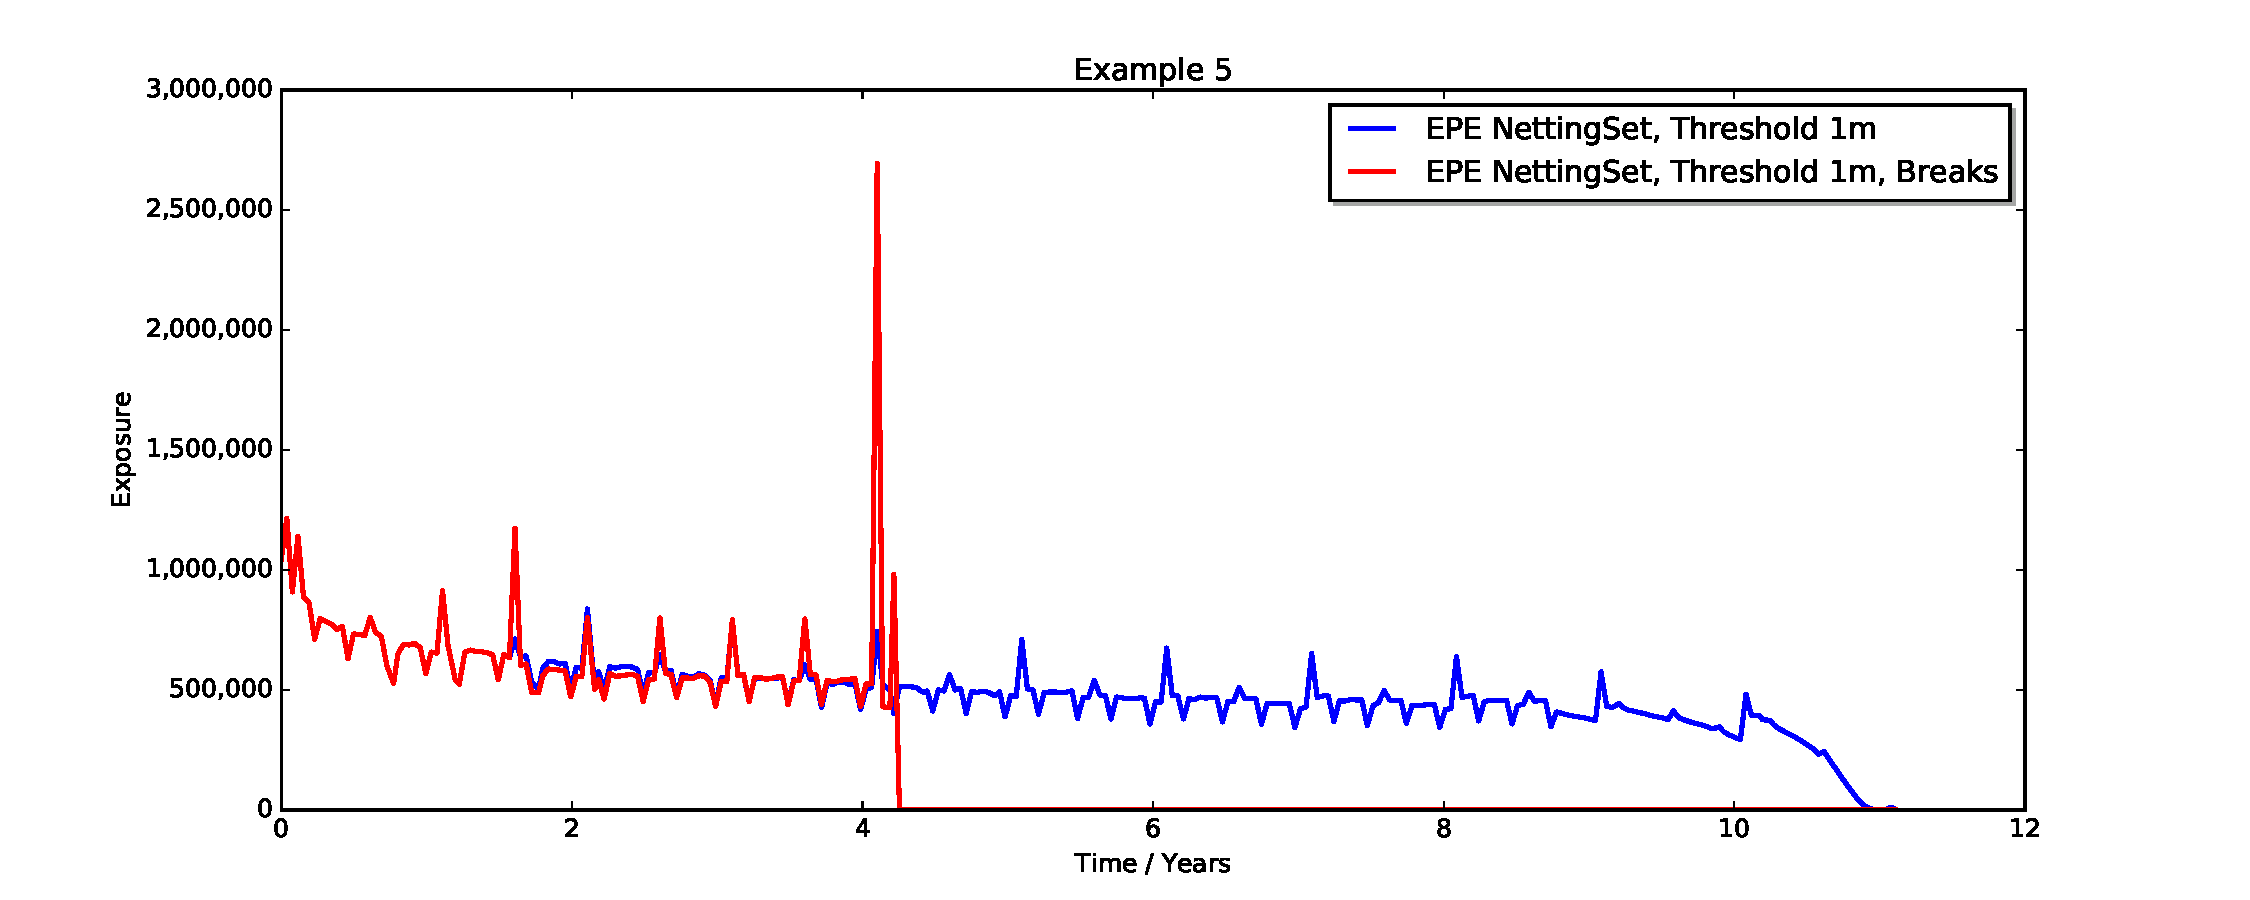
\includegraphics[scale=0.45]{mpl_threshold_break_epe.pdf}
\end{center}
\caption{Three Swaps netting set, THR=1m EUR, MTA=100k EUR, MPOR=2w. The red evolution assumes that the each trade is
  terminated at the next break date. The blue evolution ignores break dates. Simulation with 5000 paths and bi-weekly
  time steps.}
\label{fig_9}
\end{figure}

%\begin{figure}[h]
%\begin{center}
%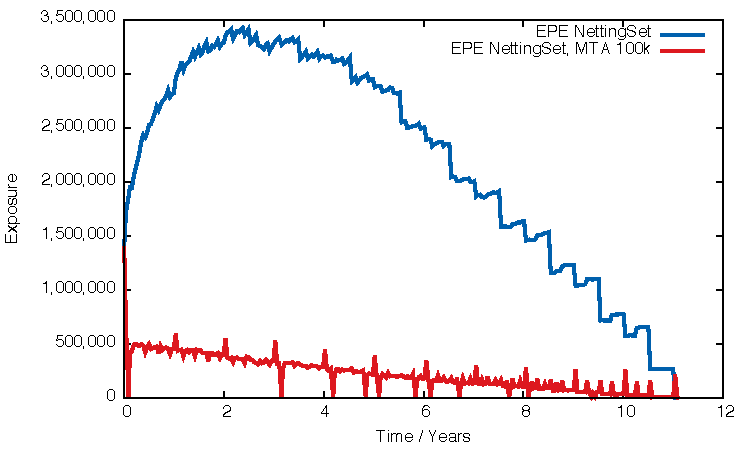
\includegraphics[scale=1.0]{example_mta_epe.pdf}
%\end{center}
%\caption{Three swaps, threshold = 0, mta > 0.}
%\label{fig_7}
%\end{figure}

\begin{figure}[h!]
\begin{center}
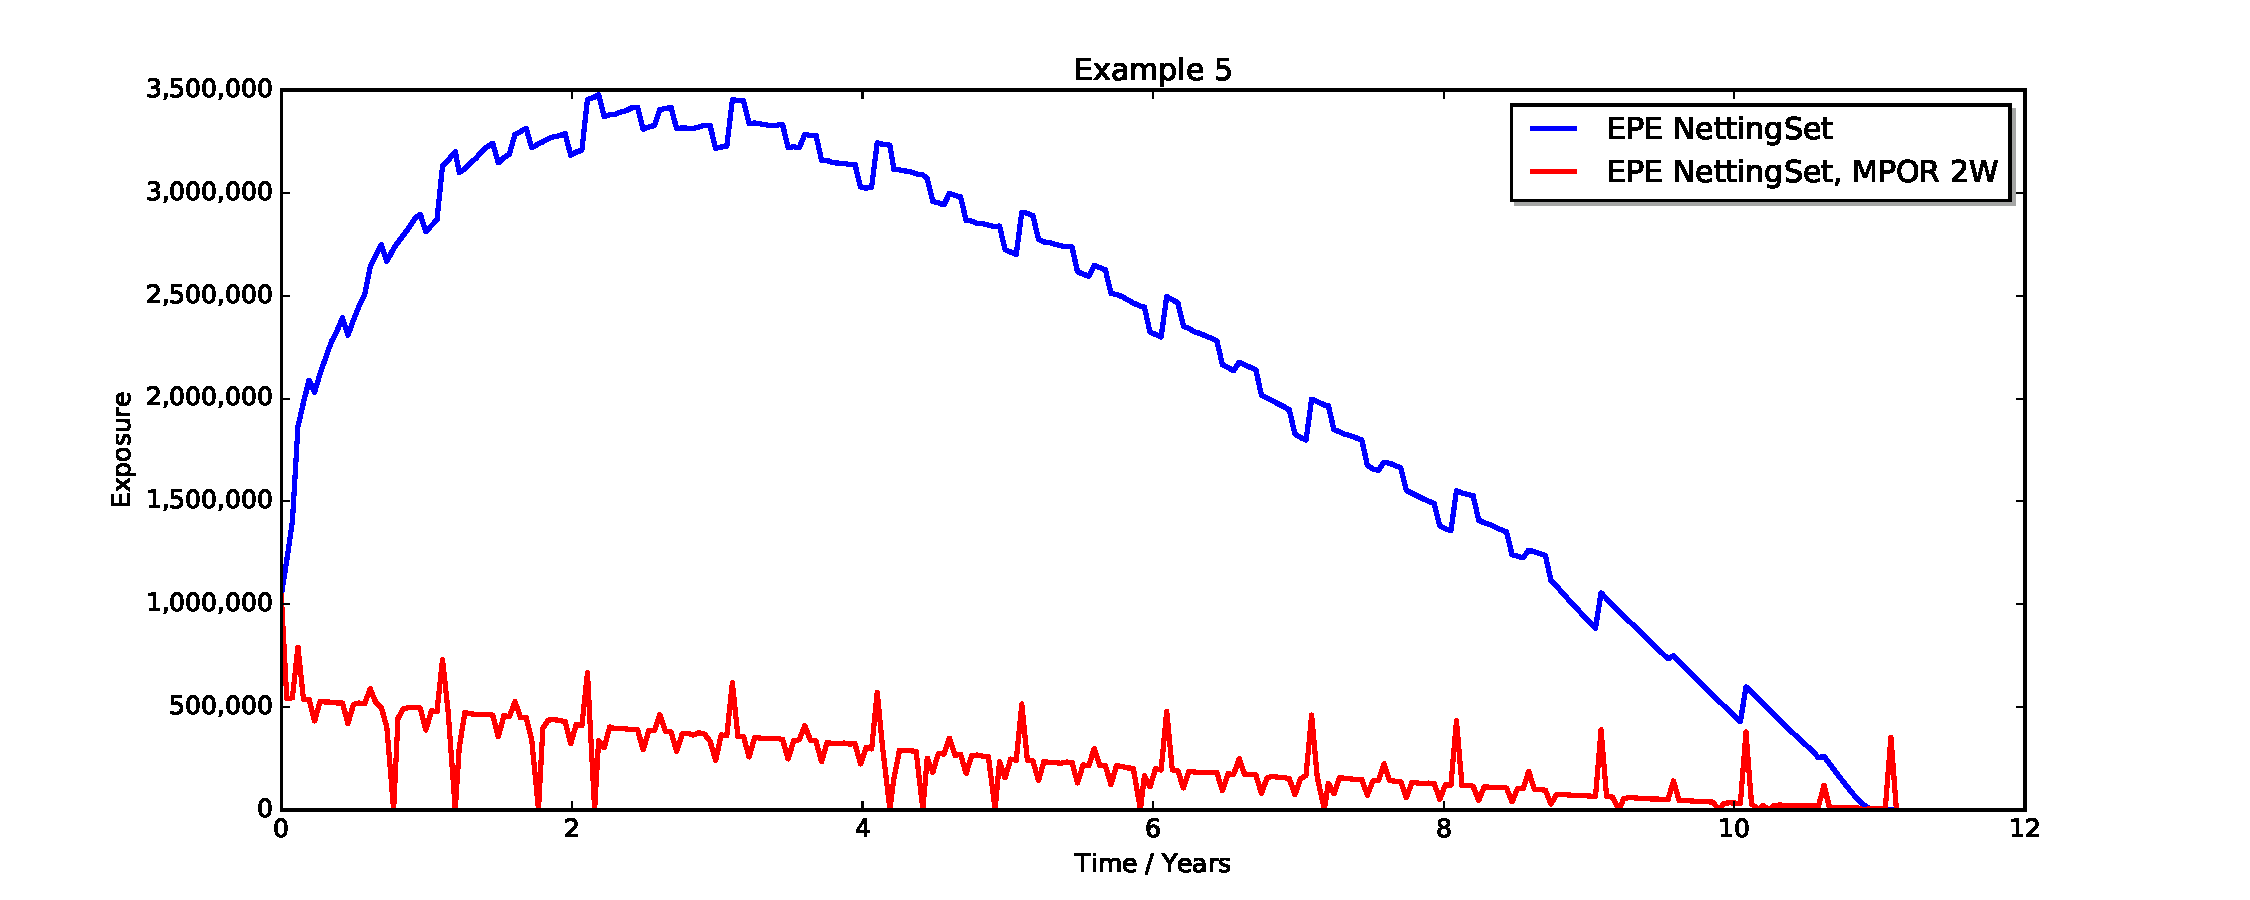
\includegraphics[scale=0.45]{mpl_mpor_epe.pdf}
\end{center}
\caption{Three Swaps, THR=MTA=0, MPOR=2w. Simulation with 5000 paths and bi-weekly time steps.}
\label{fig_10}
\end{figure}

%--------------------------------------------------------
\subsection*{CVA, DVA, FVA, COLVA, MVA, Collateral Floor}
%--------------------------------------------------------

We use one of the cases in {\tt Examples/Example\_10} to demonstrate the
XVA outputs, see folder {\tt Examples/Example\_10/Output/collateral\_threshold\_dim}.

\medskip The summary of all value adjustments (CVA, DVA, FVA, COLVA, MVA, as well as the Collateral Floor) is provided
in file {\tt xva.csv}.  The file includes the allocated CVA and DVA numbers to individual trades as introduced in the
next section. The following table illustrates the file's layout, omitting the three columns containing allocated data.

\begin{center}
\resizebox{\columnwidth}{!}{%
\begin{tabular}{|l|l|r|r|r|r|r|r|r|r|r|}
\hline
TradeId & NettingSetId & CVA & DVA & FBA & FCA & COLVA & MVA & CollateralFloor & BaselEPE & BaselEEPE \\
\hline
 & CPTY\_A &  6,521  &  151,193  & -946  &  72,103  &  2,769  & -14,203  &  189,936  &  113,260  &  1,211,770 \\
Swap\_1 & CPTY\_A &  127,688  &  211,936  & -19,624  &  100,584  &  n/a  &  n/a  &  n/a   &  2,022,590  &  2,727,010 \\
Swap\_3 & CPTY\_A &  71,315  &  91,222  & -11,270  &  43,370  &  n/a  &  n/a  &  n/a   &  1,403,320  &  2,183,860 \\
Swap\_2 & CPTY\_A &  68,763  &  100,347  & -10,755  &  47,311  &  n/a  &  n/a  &  n/a   &  1,126,520  &  1,839,590 \\
\hline
\end{tabular}
}
\end{center}

The line(s) with empty TradeId column contain values at netting set level, the others contain uncollateralised
single-trade VAs.  Note that COLVA, MVA and Collateral Floor are only available at netting set level at which collateral
is posted.

\medskip
Detailed output is written for COLVA and Collateral Floor to file {\tt colva\_nettingset\_*.csv} which shows the 
incremental contributions to these two VAs through time.


%--------------------------------------------------------
\subsection*{Exposure Reports \& XVA Allocation to Trades}
%--------------------------------------------------------
Using the example in folder {\tt Examples/Example\_10} we illustrate here the layout of an exposure report produced by
ORE. The report shows the exposure evolution of Swap\_1 without collateral which - after running Example\_10 - is found
in folder \\
{\tt Examples/Example\_10/Output/collateral\_none/exposure\_trade\_Swap\_1.csv}:

\begin{center}
\resizebox{\columnwidth}{!}{%
\begin{tabular}{|l|l|r|r|r|r|r|r|r|r|}
\hline
TradeId & Date & Time & EPE & ENE & AllocEPE & AllocENE & PFE & BaselEE & BaselEEE \\
\hline
Swap\_1 & 05/02/16 & 0.0000 & 0  & 1,711,748  & 0  & 0  & 0  & 0  & 0 \\
Swap\_1 & 19/02/16 & 0.0383 & 38,203   & 1,749,913  & -1,200,677 & 511,033 & 239,504 & 38,202 & 38,202 \\
Swap\_1 & 04/03/16 & 0.0765 & 132,862  & 1,843,837 & -927,499 & 783,476 & 1,021,715 & 132,845 & 132,845 \\
%Swap\_1 & 18/03/16 & 0.1148 & 299,155  & 1,742,450  & -650,225  & 793,067  & 1,914,150  & 299,091  & 299,091 \\
%Swap\_1 & 01/04/16 & 0.1530 & 390,178  & 1,834,810  & -552,029  & 892,604  & 2,373,560  & 390,058  & 390,058 \\
%Swap\_1 & 15/04/16 & 0.1913 & 471,849  & 1,918,600  & -465,580  & 981,171  & 2,765,710  & 471,659  & 471,659 \\
%Swap\_1 & 29/04/16 & 0.2295 & 550,301  & 2,000,640  & -330,578  & 1,119,760  & 3,106,810  & 550,016  & 550,016 \\
%Swap\_1 & 13/05/16 & 0.2678 & 620,279  & 2,074,880  & -266,042  & 1,188,560  & 3,427,080  & 619,888  & 619,888 \\
%Swap\_1 & 27/05/16 & 0.3060 & 690,018  & 2,140,320  & -190,419  & 1,259,880  & 3,778,570  & 689,509  & 689,509 \\
%Swap\_1 & 10/06/16 & 0.3443 & 763,207  & 2,206,020  & -137,681  & 1,305,130  & 4,052,870  & 762,560  & 762,560 \\
Swap\_1 & ... & ...& ... & ... & ... & ... & ... & ... & ... \\
\hline
\end{tabular}
}
\end{center}

The exposure measures EPE, ENE and PFE, and the Basel exposure measures $EE_B$ and $EEE_B$, are defined in appendix
\ref{sec:app_exposure}. Allocated exposures are defined in appendix \ref{sec:app_allocation}. The PFE quantile and
allocation method are chosen as described in section \ref{sec:analytics}. \\

In addition to single trade exposure files, ORE produces an exposure file per netting set. The example from the same
folder as above is:

\begin{center}
\resizebox{\columnwidth}{!}{%
\begin{tabular}{|l|l|r|r|r|r|r|r|r|}
\hline
NettingSet & Date & Time & EPE & ENE & PFE & ExpectedCollateral & BaselEE & BaselEEE \\
\hline
CPTY\_A & 05/02/16 & 0.0000 & 1,203,836 & 0 & 1,203,836 & 0 & 1,203,836 & 1,203,836 \\%1,211,770 & 0 & 1,211,770 & 0 & 1,211,770 & 1,211,770\\
CPTY\_A & 19/02/16 & 0.0383 & 1,337,713 & 137,326 & 3,403,460 & 0 & 1,337,651 & 1,337,651 \\ %0.0383 & 1,344,220 & 137,776 & 3,414,000 & 0 & 1,344,160 & 1,344,160\\
%CPTY\_A & 04/03/16 & 0.0765 & 1,518,610 & 308,381 & 4,354,060 & 0 & 1,518,410 & 1,518,410\\
%CPTY\_A & 18/03/16 & 0.1148 & 1,846,900 & 382,068 & 5,200,730 & 0 & 1,846,500 & 1,846,500\\
%CPTY\_A & 01/04/16 & 0.1530 & 1,961,290 & 494,416 & 5,869,470 & 0 & 1,960,690 & 1,960,690\\
%CPTY\_A & 15/04/16 & 0.1913 & 2,067,240 & 598,283 & 6,384,140 & 0 & 2,066,400 & 2,066,400\\
%CPTY\_A & 29/04/16 & 0.2295 & 2,053,670 & 745,960 & 6,740,070 & 0 & 2,052,610 & 2,066,400\\
%CPTY\_A & 13/05/16 & 0.2678 & 2,149,190 & 845,507 & 6,930,230 & 0 & 2,147,840 & 2,147,840\\
%CPTY\_A & 27/05/16 & 0.3060 & 2,235,630 & 930,218 & 7,295,440 & 0 & 2,233,980 & 2,233,980\\
%CPTY\_A & 10/06/16 & 0.3443 & 2,314,470 & 1,014,690 & 7,753,190 & 0 & 2,312,510 & 2,312,510\\
CPTY\_A & ... & ...& ... & ... & ... & ... & ... & ...\\
%CPTY\_A & 07/07/17 & 1.4167 & 3,320,430 & 2,423,890 & 12,787,900 & 0 & 3,304,650 & 3,304,650\\
%CPTY\_A & 21/07/17 & 1.4551 & 3,351,780 & 2,452,640 & 12,964,200 & 0 & 3,335,420 & 3,335,420\\
%CPTY\_A & 04/08/17 & 1.4934 & 3,302,820 & 2,511,500 & 12,796,100 & 0 & 3,286,260 & 3,335,420\\
%CPTY\_A & 18/08/17 & 1.5318 & 3,339,840 & 2,545,850 & 13,120,000 & 0 & 3,322,640 & 3,335,420\\
%CPTY\_A & 01/09/17 & 1.5701 & 3,371,300 & 2,576,100 & 13,238,700 & 0 & 3,353,480 & 3,353,480\\
%CPTY\_A & 15/09/17 & 1.6085 & 3,279,670 & 2,555,370 & 13,041,300 & 0 & 3,261,880 & 3,353,480\\
%CPTY\_A & 29/09/17 & 1.6468 & 3,305,060 & 2,579,200 & 13,072,800 & 0 & 3,286,680 & 3,353,480\\
%CPTY\_A & 13/10/17 & 1.6852 & 3,332,830 & 2,604,200 & 13,225,600 & 0 & 3,313,850 & 3,353,480\\
%CPTY\_A & 27/10/17 & 1.7236 & 3,280,280 & 2,661,770 & 13,034,600 & 0 & 3,261,150 & 3,353,480\\
%CPTY\_A & 13/11/17 & 1.7701 & 3,316,800 & 2,701,060 & 13,331,600 & 0 & 3,296,880 & 3,353,480\\
%CPTY\_A & 24/11/17 & 1.8003 & 3,337,760 & 2,720,870 & 13,402,400 & 0 & 3,317,280 & 3,353,480\\
%CPTY\_A & ... & ...& ... & ... & ... & ... & ... & ...\\
\hline
\end{tabular}
}
\end{center}

Allocated exposures are missing here, as they make sense at the trade level only, and the expected collateral balance is
added for information (in this case zero as collateralisation is deactivated in this example).

\medskip The allocation of netting set exposure and XVA to the trade level is frequently required by finance
departments. This allocation is also featured in {\tt Examples/Example\_10}. We start again with the uncollateralised
case in figure \ref{fig_12}, followed by the case with threshold 1m EUR in figure \ref{fig_13}.
\begin{figure}[h!]
\begin{center}
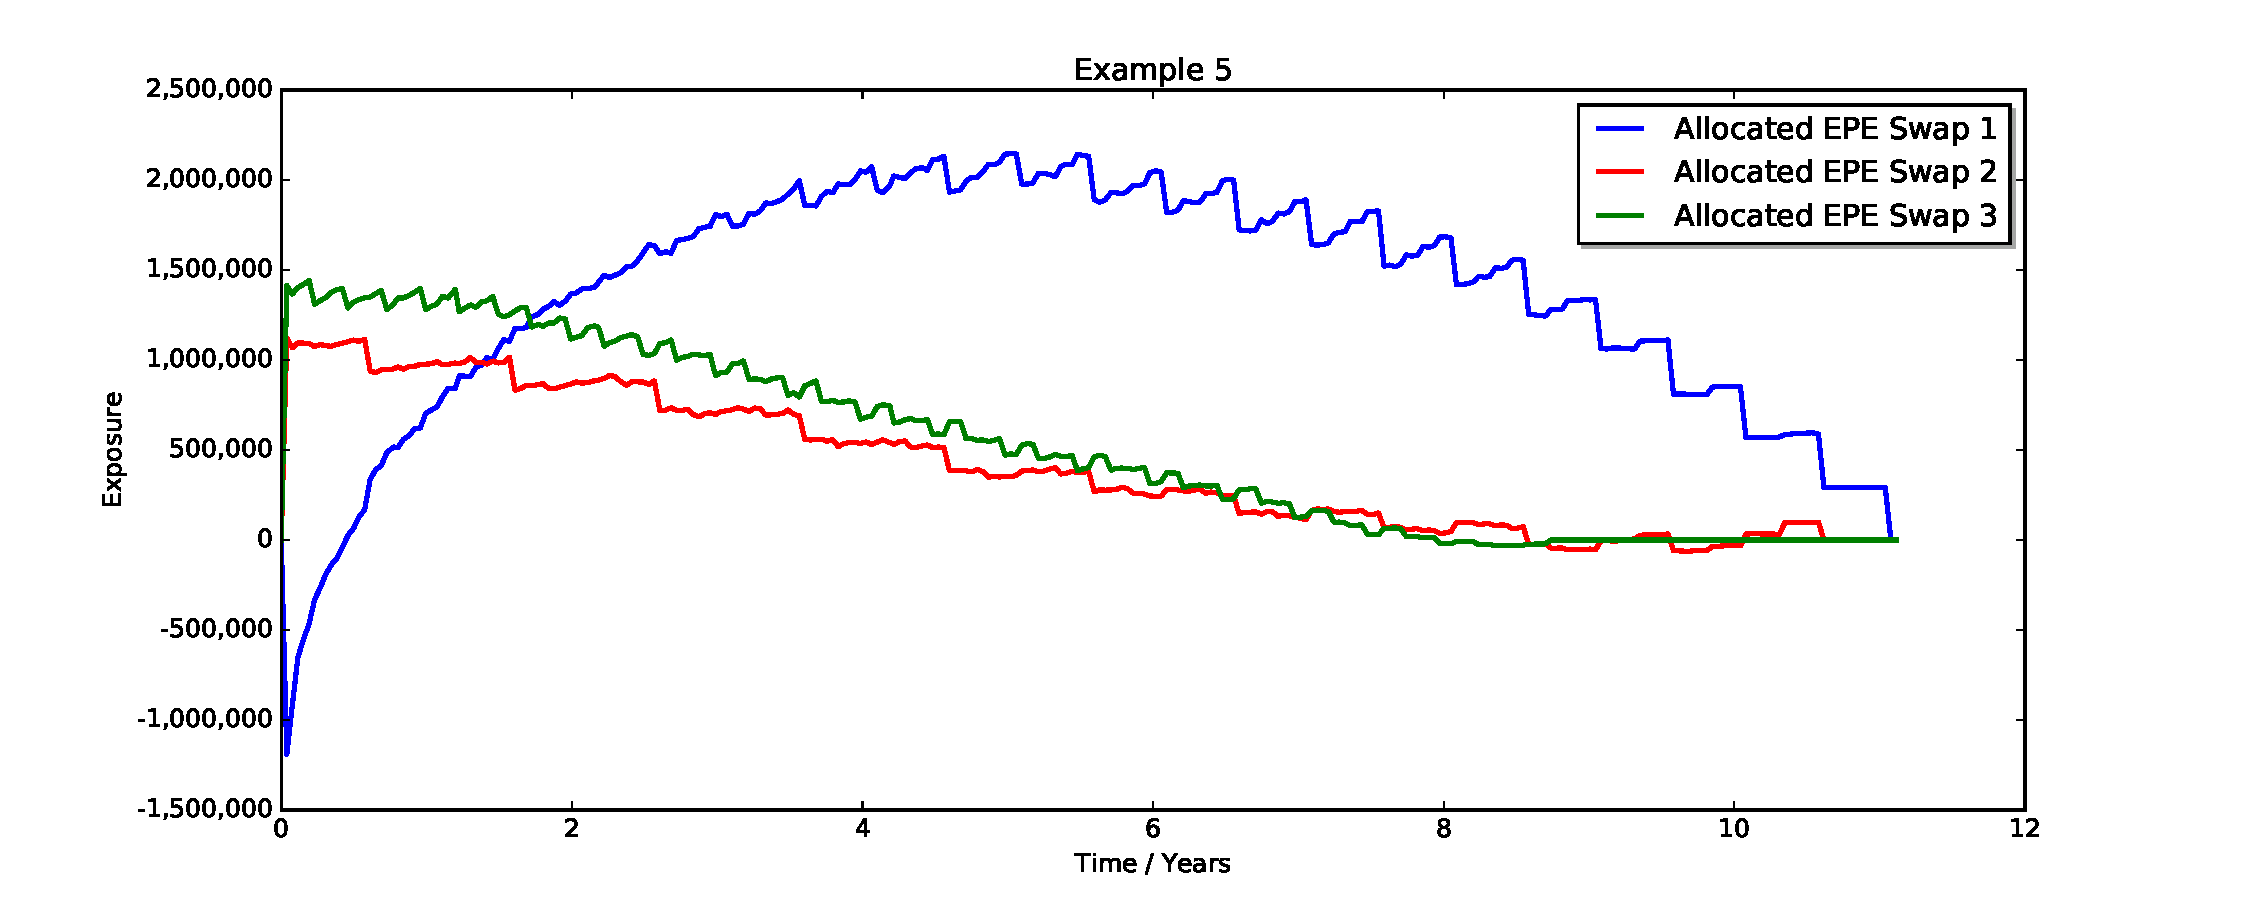
\includegraphics[scale=0.45]{mpl_nocollateral_allocated_epe.pdf}
\end{center}
\caption{Exposure allocation without collateral. Simulation with 5000 paths and bi-weekly time steps.}
\label{fig_12}
\end{figure}
In both cases we apply the {\em marginal} (Euler) allocation method as published by Pykhtin and Rosen in 2010, hence we
see the typical negative EPE for one of the trades at times when it reduces the netting set exposure. The case with
collateral moreover shows the typical spikes in the allocated exposures.
\begin{figure}[h!]
\begin{center}
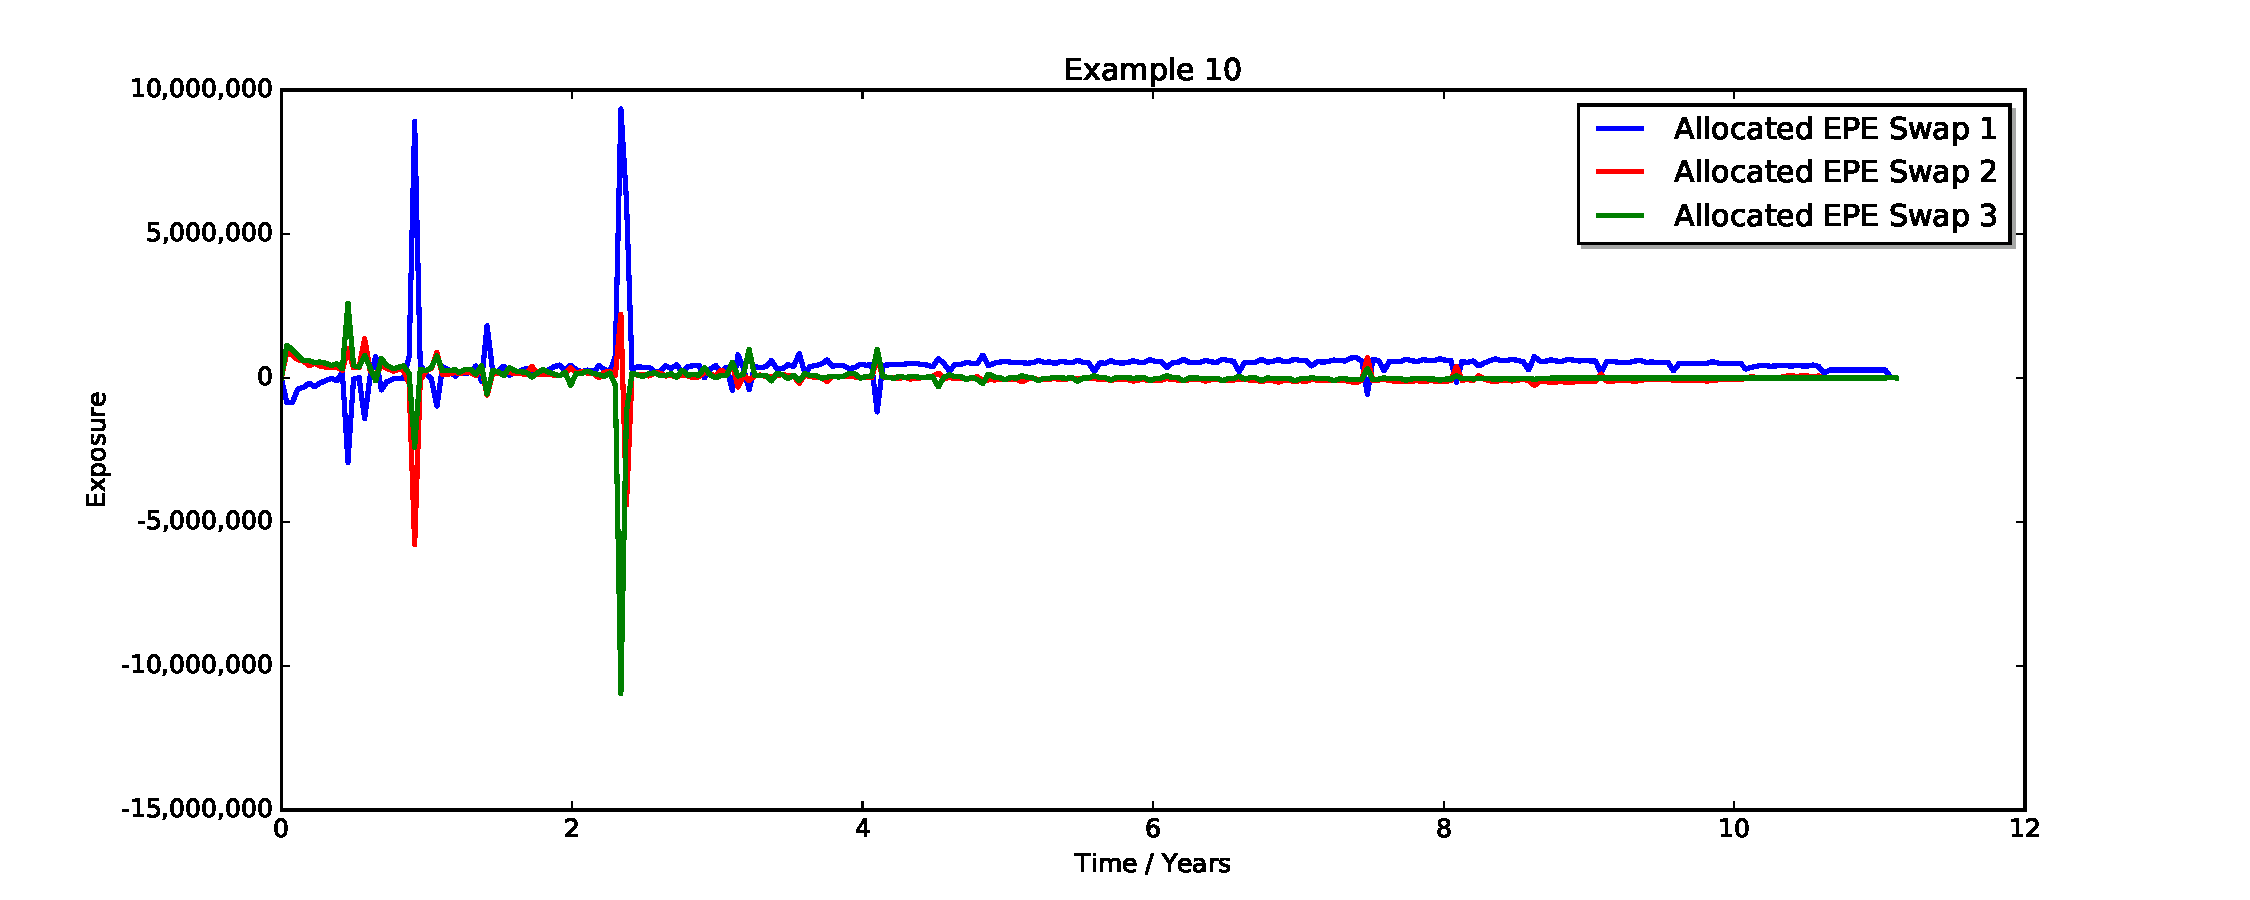
\includegraphics[scale=0.45]{mpl_threshold_allocated_epe.pdf}
\end{center}
\caption{Exposure allocation with collateral and threshold 1m EUR. Simulation with 5000 paths and bi-weekly time steps.}
\label{fig_13}
\end{figure}
The analytics results also feature allocated XVAs in file {\tt xva.csv} which are derived from the allocated exposure
profiles. Note that ORE also offers alternative allocation methods to the marginal method by Pykhtin/Rosen, which can be
explored with {\tt Examples/Example\_10}.

%--------------------------------------------------------
\subsection{Basel Exposure Measures}\label{sec:basel}
%--------------------------------------------------------

Example {\tt Example\_11} demonstrates the relation between the evolution of the expected exposure (EPE in our notation)
to the `Basel' exposure measures EE\_B, EEE\_B, EPE\_B and EEPE\_B as defined in appendix \ref{sec:app_exposure}. In
particular the latter is used in internal model methods for counterparty credit risk as a measure for the exposure at
default. It is a `derivative' of the expected exposure evolution and defined as a time average over the running maximum
of EE\_B up to the horizon of one year.
\begin{figure}[h!]
\begin{center}
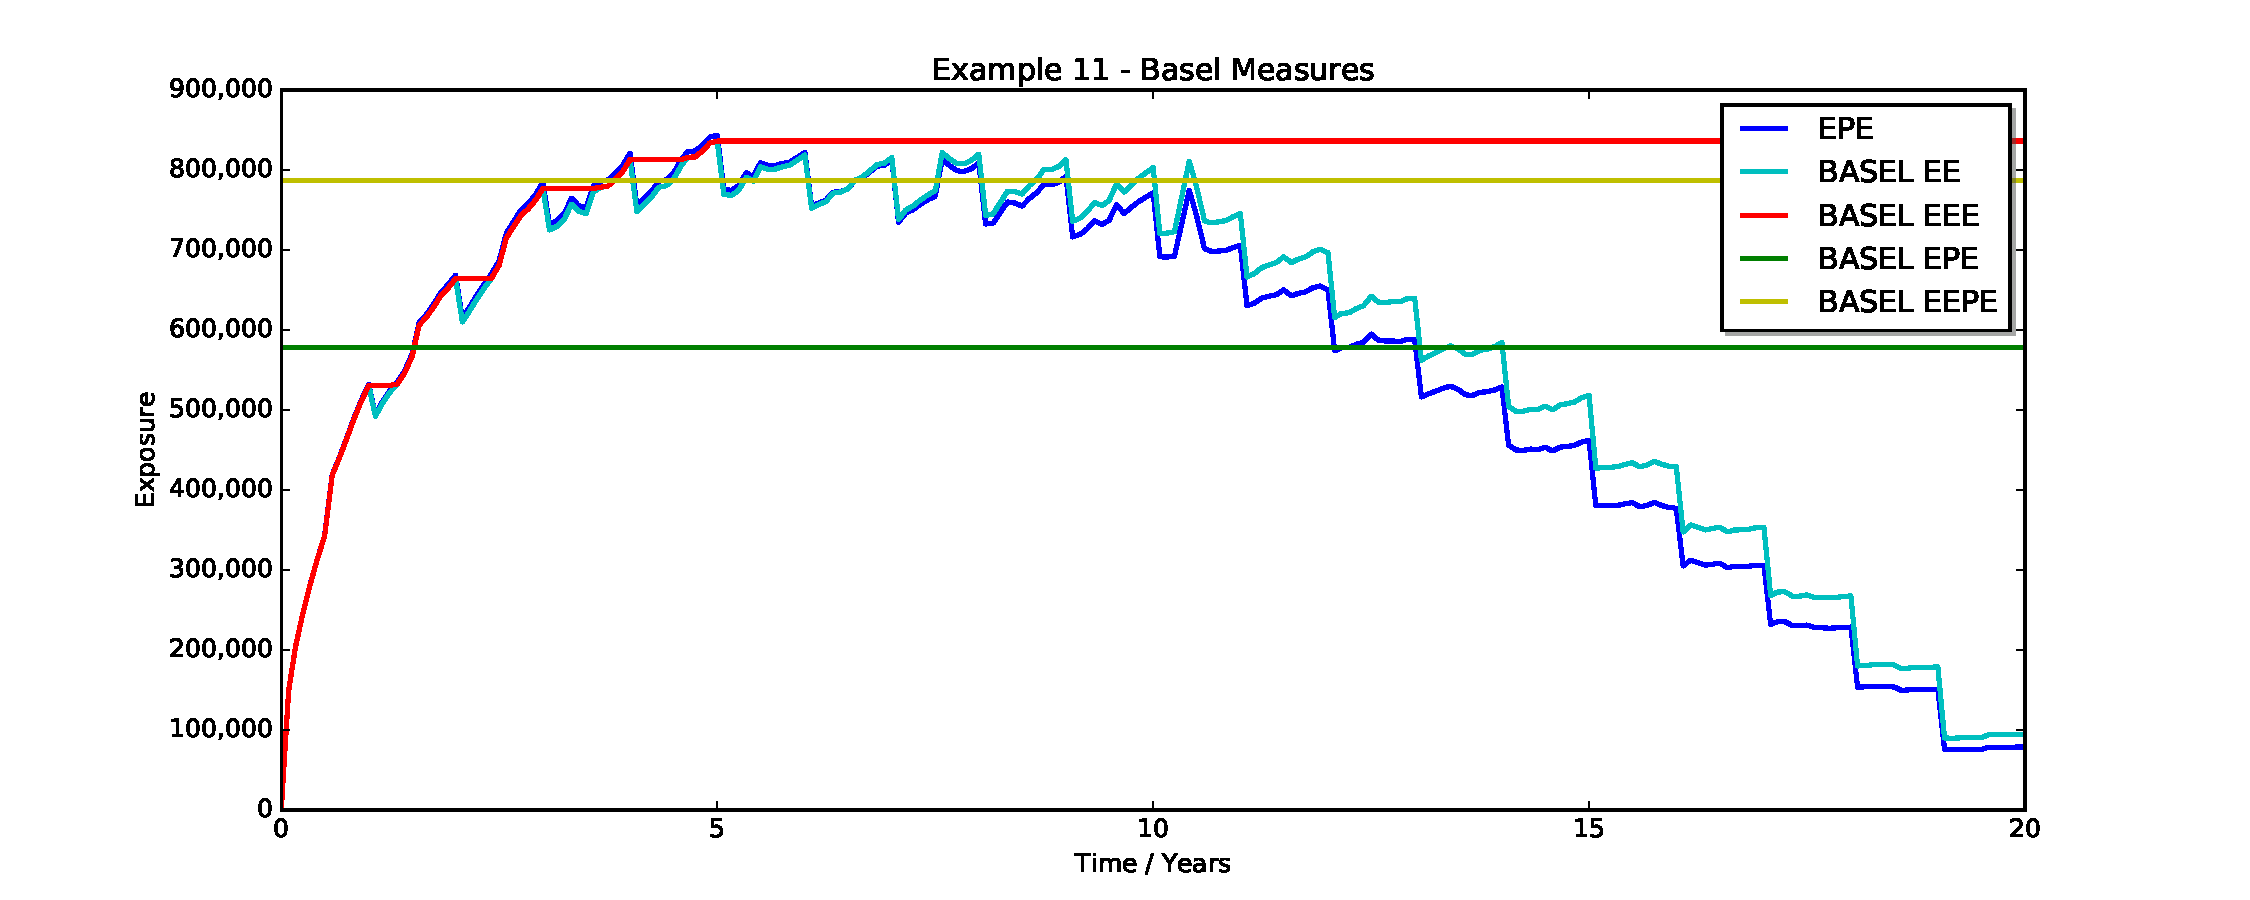
\includegraphics[scale=0.45]{mpl_basel_exposures.pdf}
\end{center}
\caption{Evolution of the expected exposure of Vanilla Swap, comparison to the `Basel' exposure measures EEE\_B, EPE\_B and EEPE\_B. Note that the latter two are indistinguishable in this case, because the expected exposure is increasing for the first year.}
\label{fig_14}
\end{figure}

%--------------------------------------------------------
\subsection{Long Term Simulation with Horizon Shift}\label{sec:longterm}
%--------------------------------------------------------

The example in folder {\tt Example\_12} finally demonstrates an effect that, at first glance, seems to cause a serious
issue with long term simulations. Fortunately this can be avoided quite easily in the Linear Gauss Markov model setting
that is used here. \\

In the example we consider a Swap with maturity in 50 years in a flat yield curve environment. If we simulate this
naively as in all previous cases, we obtain a particularly noisy EPE profile that does not nearly reconcile with the
known exposure (analytical Swaption prices). This is shown in figure \ref{fig_15} (`no horizon shift'). The origin of
this issue is the width of the risk-neutral NPV distribution at long time horizons which can turn out to be quite small
so that the Monte Carlo simulation with finite number of samples does not reach far enough into the positive or negative
NPV range to adequately sample the distribution, and estimate both EPE and ENE in a single run.  Increasing the number
of samples may not solve the problem, and may not even be feasible in a realistic setting. \\

The way out is applying a `shift transformation' to the Linear Gauss Markov model, see {\tt
  Example\_12/Input/simulation2.xml} in lines 92-95:
\begin{listing}[H]
%\hrule\medskip
\begin{minted}[fontsize=\footnotesize]{xml}
        <ParameterTransformation>
          <ShiftHorizon>30.0</ShiftHorizon>
          <Scaling>1.0</Scaling>
        </ParameterTransformation>
\end{minted}
%\hrule
%\caption{LGM Shift transformation}
%\label{lst:shift_transformation}
\end{listing}

The effect of the 'ShiftHorizon' parameter $T$ is to apply a shift to the Linear Gauss Markov model's $H(t)$ parameter
(see appendix \ref{sec:app_rfe}) {\em after} the model has been calibrated, i.e. to replace:
$$ 
H(t) \rightarrow H(t) - H(T) 
$$ 
It can be shown that this leaves all expectations computed in the model (such as EPE and ENE) invariant. As explained in
\cite{Lichters}, subtracting an $H$ shift effectively means performing a change of measure from the `native' LGM measure
to a T-Forward measure with horizon $T$, here 30 years. Both negative and positive shifts are permissible, but only
negative shifts are connected with a T-Forward measure and improve numerical stability. \\

In our experience it is helpful to place the horizon in the middle of the portfolio duration to significantly improve
the quality of long term expectations. The effect of this change (only) is shown in the same figure \ref{fig_15}
(`shifted horizon').
\begin{figure}[h!]
\begin{center}
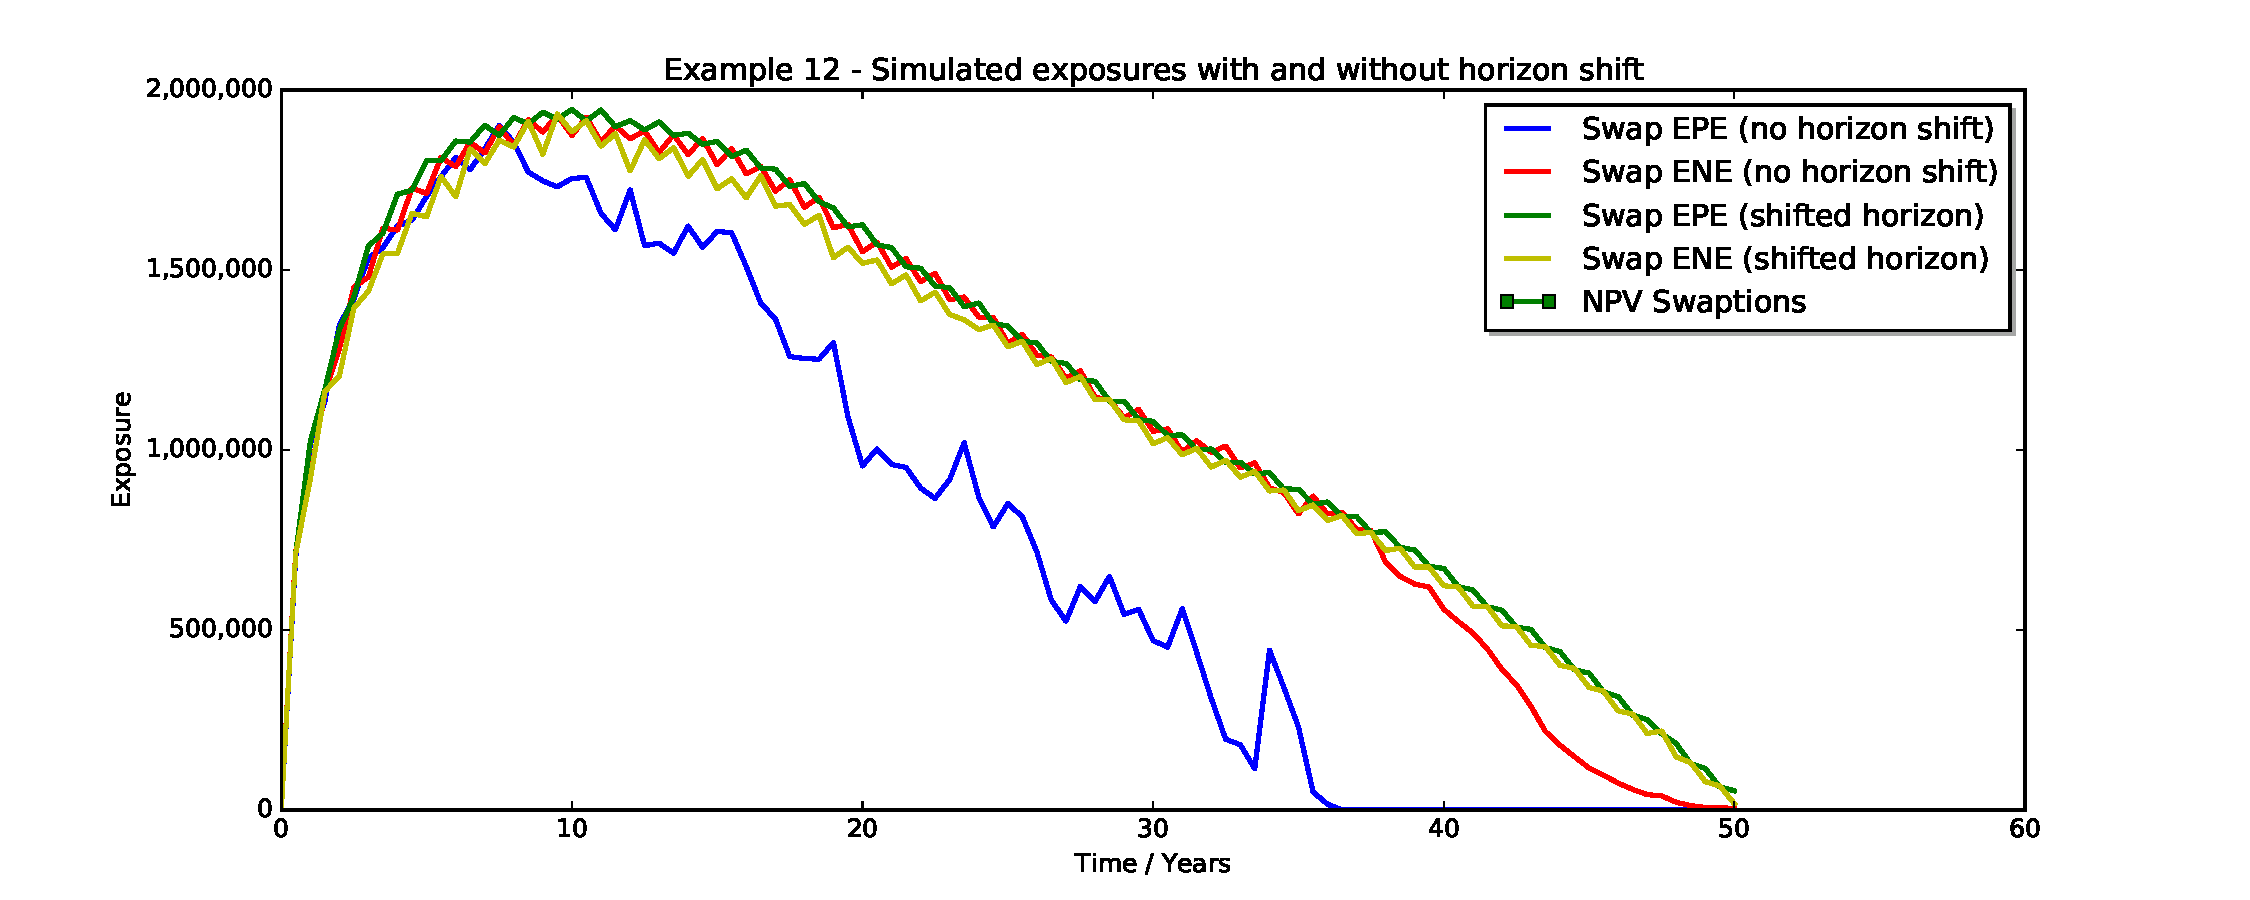
\includegraphics[scale=0.45]{mpl_longterm.pdf}
\end{center}
\caption{Long term Swap exposure simulation with and without horizon shift.}
\label{fig_15}
\end{figure}
Figure \ref{fig_15b} further illustrates the origin of the problem and its resolution: The rate distribution's mean
(without horizon shift or change of measure) drifts upwards due to convexity effects (note that the yield curve is flat
in this example), and the distribution's width is then too narrow at long horizons to yield a sufficient number of low
rate scenarios with contributions to the Swap's $\EPE$ (it is a floating rate payer). With the horizon shift (change of
measure), the distribution's mean is pulled 'back' at long horizons, because the convexity effect is effectively wiped
out at the chosen horizon, and the expected rate matches the forward rate.

\begin{figure}[h!]
\begin{center}
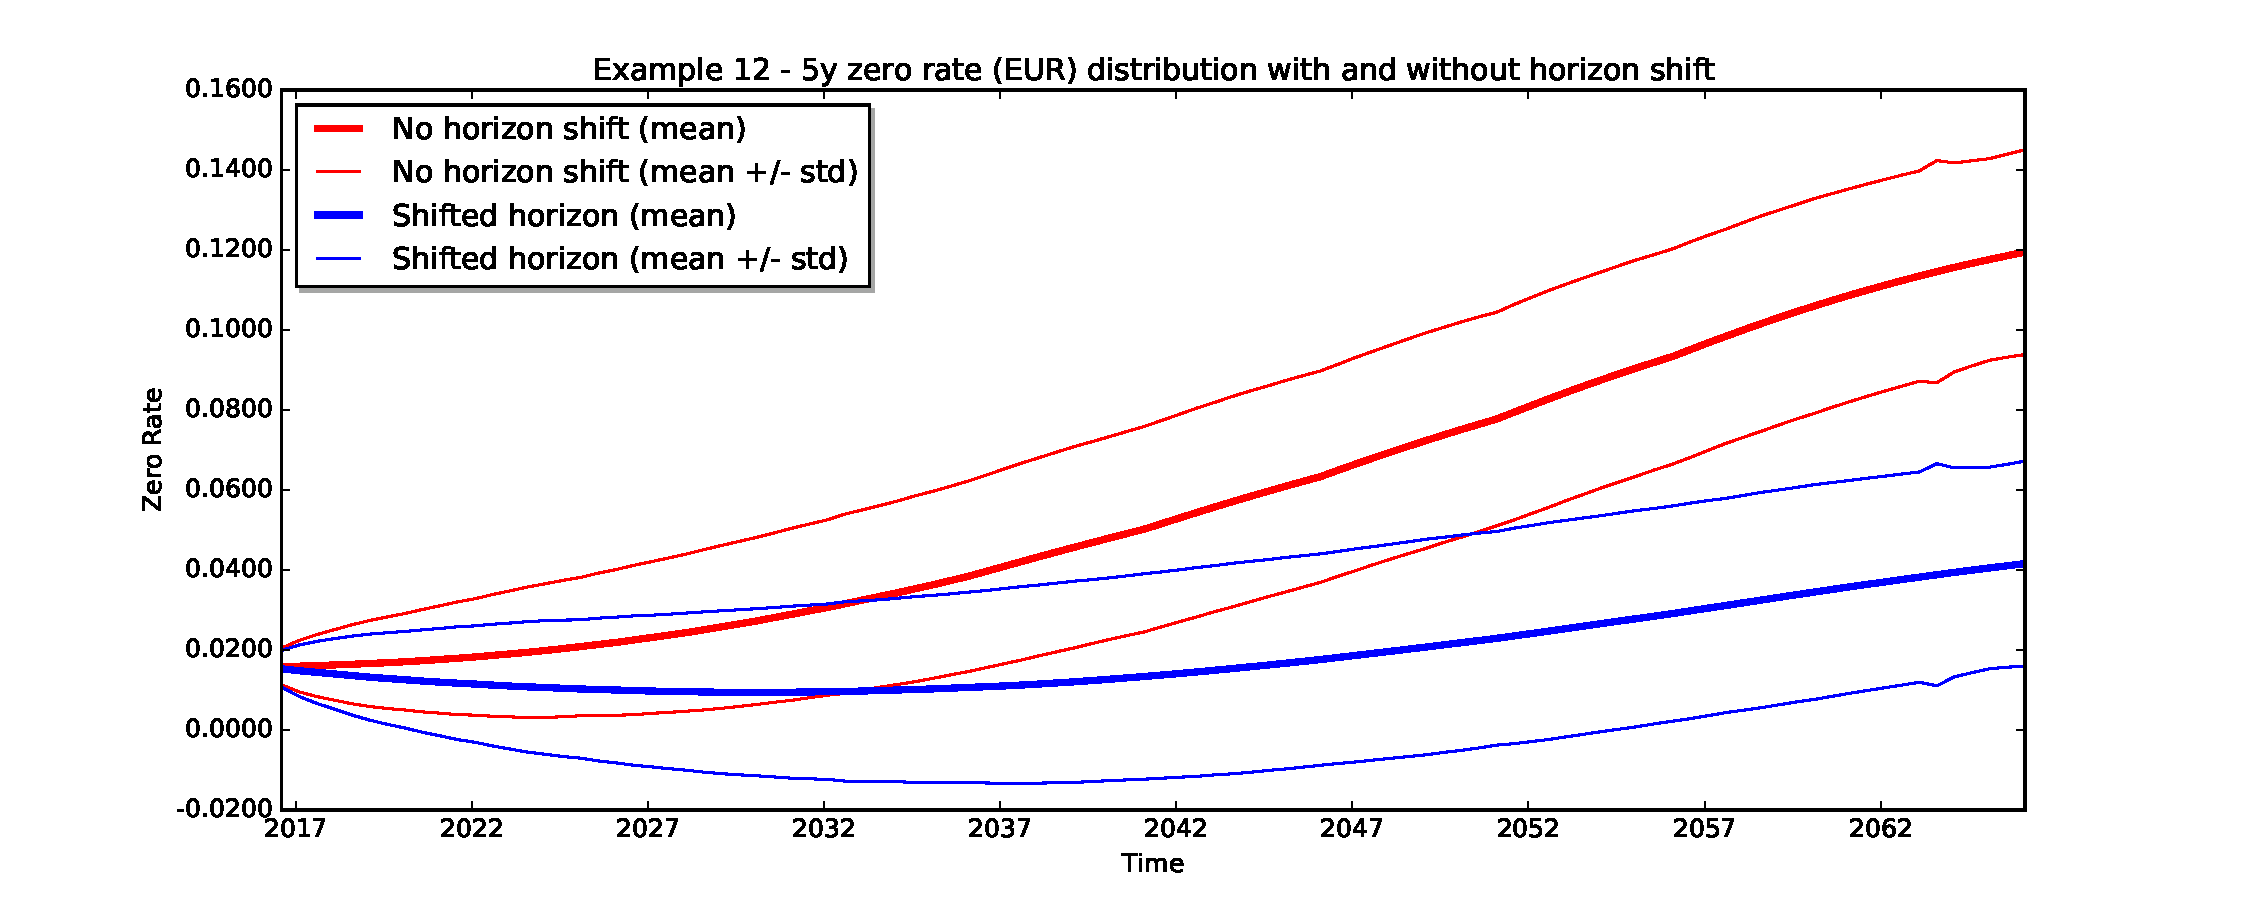
\includegraphics[scale=0.45]{mpl_rates.pdf}
\end{center}
\caption{Evolution of rate distributions with and without horizon shift (change of measure). Thick lines indicate mean
  values, thin lines are contours of the rate distribution at $\pm$ one standard deviation.}
\label{fig_15b}
\end{figure}

%--------------------------------------------------------
\subsection{Dynamic Initial Margin and MVA}\label{sec:dim}
%--------------------------------------------------------

This example in folder {\tt Examples/Example\_13} demonstrates Dynamic Initial Margin calculations (see also appendix
\ref{sec:app_dim}) for a number of elementary products:
\begin{itemize}
\item A single currency Swap in EUR (case A), 
\item a European Swaption in EUR with physical delivery (case B), 
\item a single currency Swap in USD (case C), and 
\item a EUR/USD cross currency Swap (case D).
\end{itemize}

The examples can be run as before with 

\medskip
\centerline{\tt python run\_A.py} 

\medskip
and likewise for cases B, C and D. The essential results of each run are are visualised in the form of 
\begin{itemize}
\item evolution of expected DIM
\item regression plots at selected future times 
\end{itemize}
illustrated for cases A and B in figures \ref{fig_ex13a_evolution} - \ref{fig_ex13b_regression}. 
In the three swap cases, the regression orders do make a noticeable difference in the respective expected DIM evolution. In the Swaption case B, first and second order polynomial choice makes a difference before option expiry. More details on this DIM model and its performance can be found in \cite{Anfuso2016,LichtersEtAl}.
 
\begin{figure}[h!]
\begin{center}
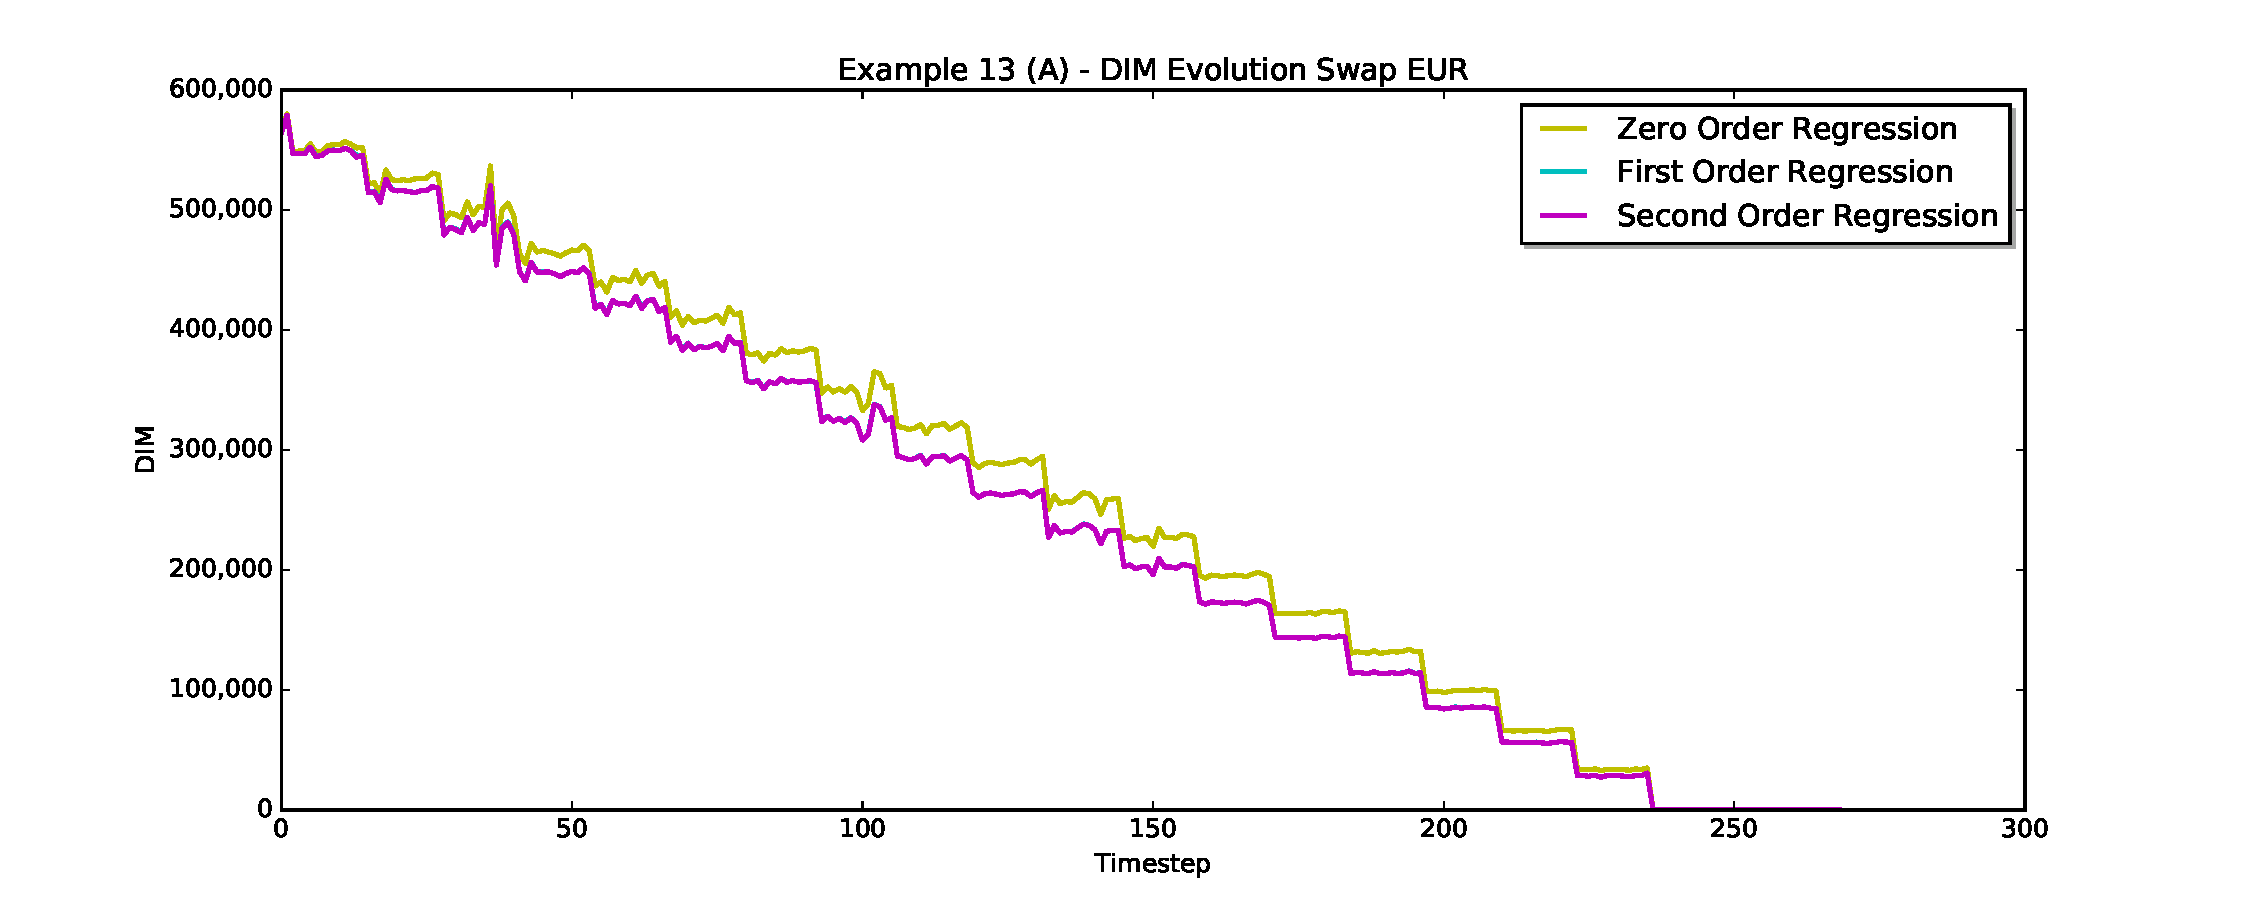
\includegraphics[scale=0.45]{mpl_dim_evolution_A_swap_eur.pdf}
\end{center}
\caption{Evolution of expected Dynamic Initial Margin (DIM) for the EUR Swap of Example 13 A. DIM is evaluated using
  regression of NPV change variances versus the simulated 3M Euribor fixing; regression polynomials are zero, first and
  second order (first and second order curves are not distinguishable here). The simulation uses 1000 samples and a time
  grid with bi-weekly steps in line with the Margin Period of Risk.}
\label{fig_ex13a_evolution}
\end{figure}

\begin{figure}[h!]
\begin{center}
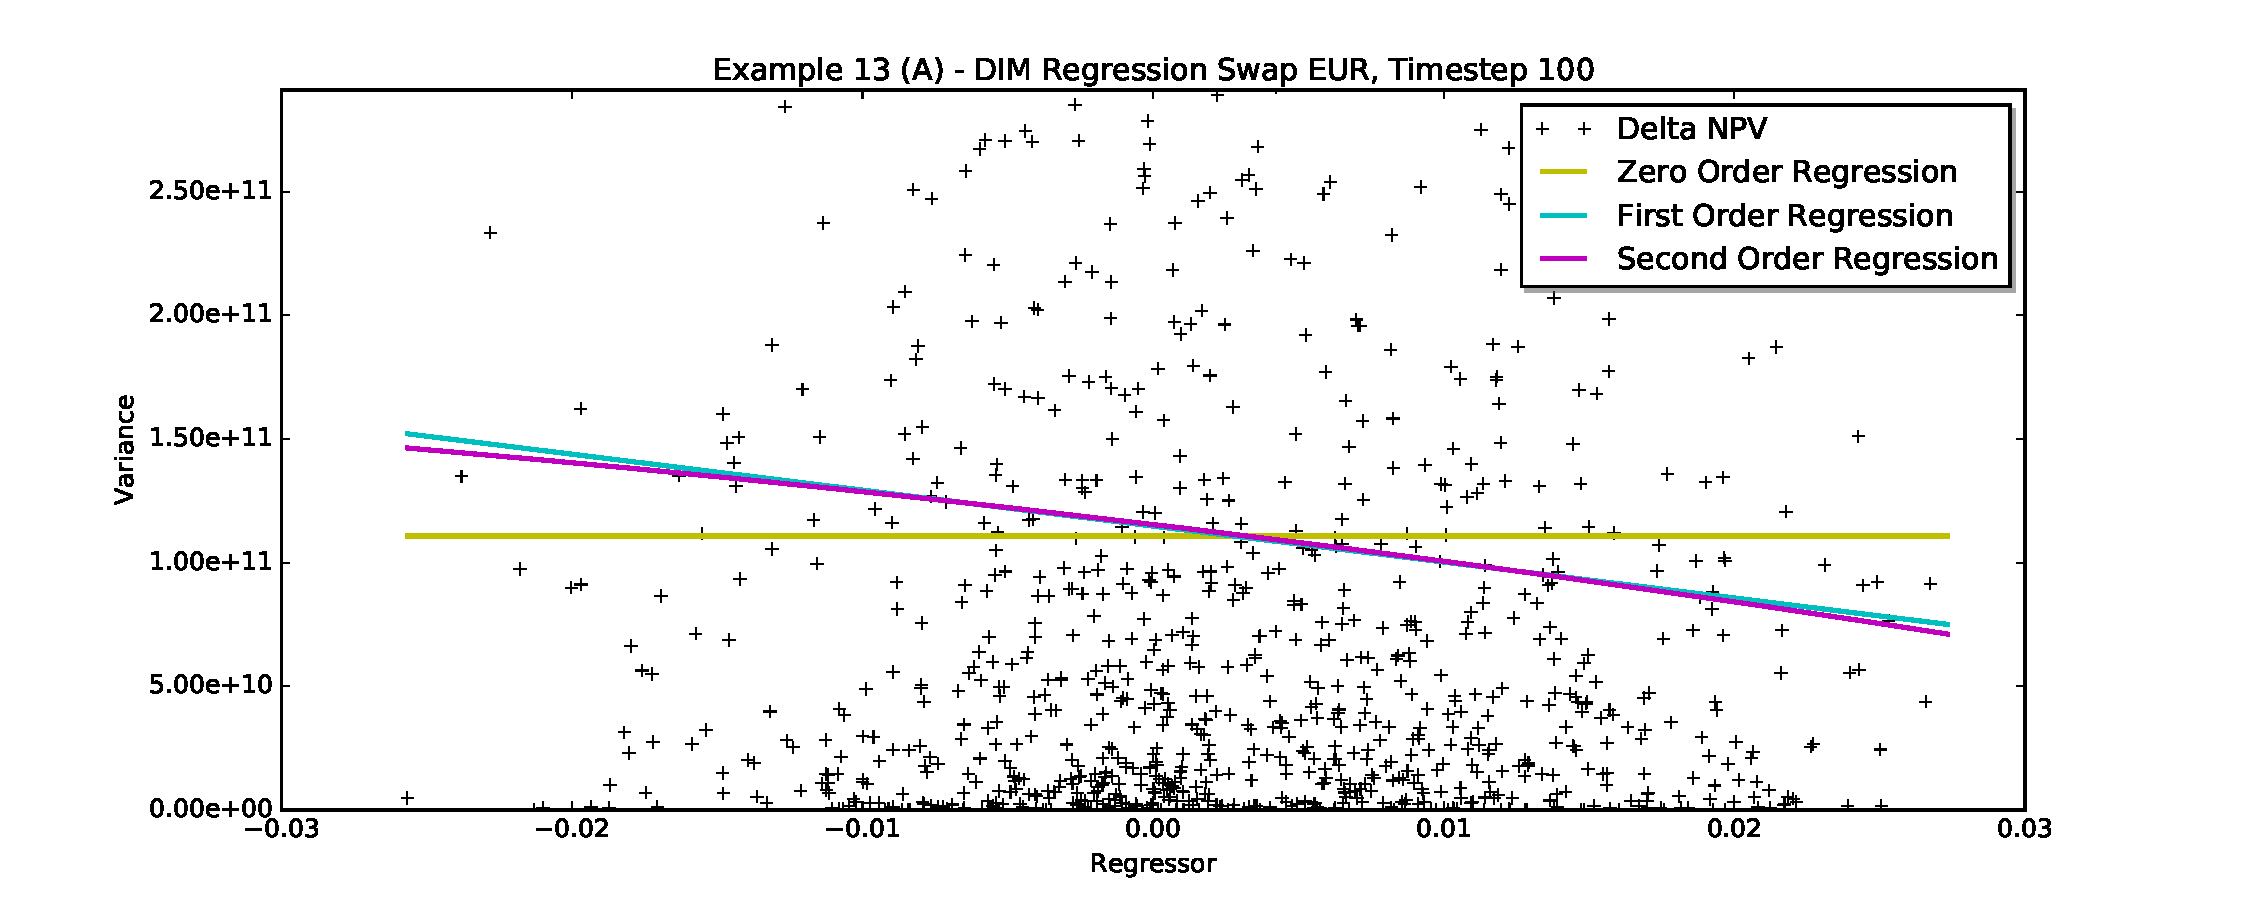
\includegraphics[scale=0.45]{mpl_dim_regression_A_swap_eur.pdf}
\end{center}
\caption{Regression snapshot at time step 100 for the EUR Swap of Example 13 A.}
\label{fig_ex13a_regression}
\end{figure}

\begin{figure}[h!]
\begin{center}
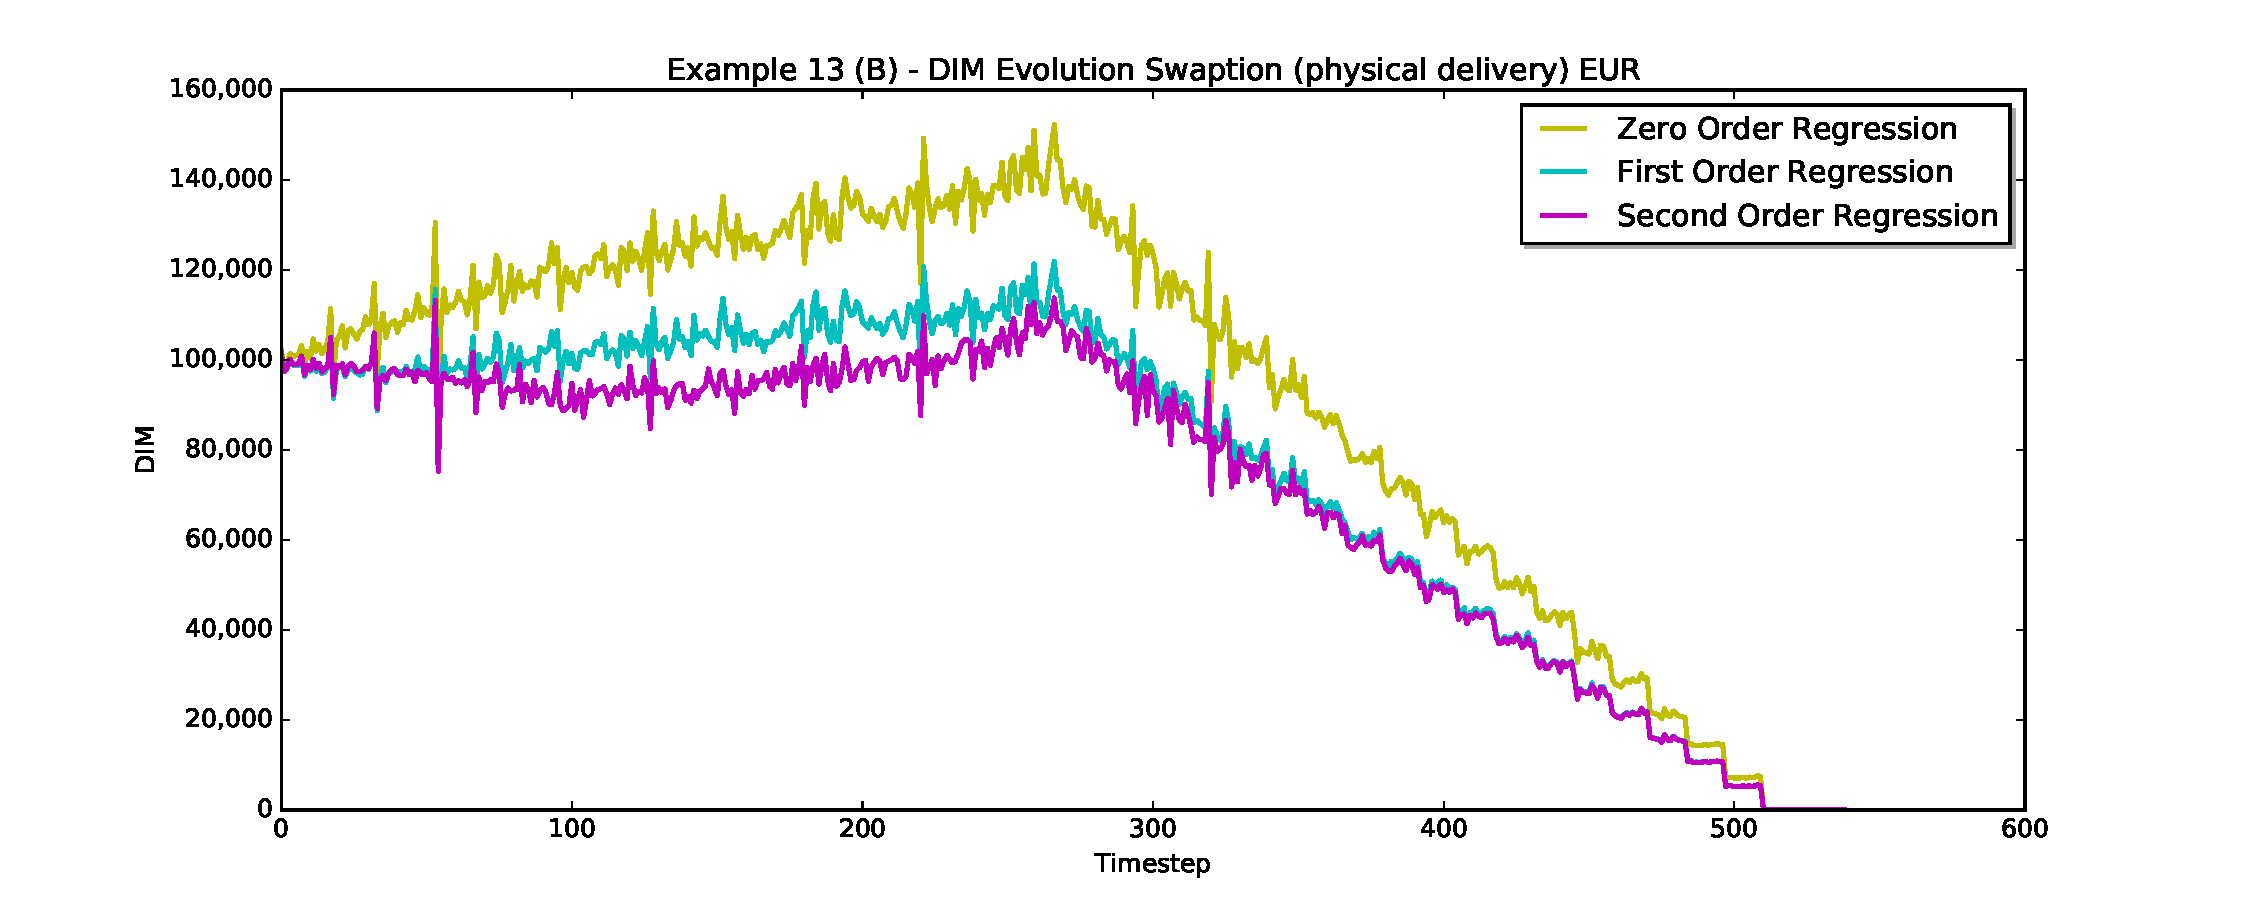
\includegraphics[scale=0.45]{mpl_dim_evolution_B_swaption_eur.pdf}
\end{center}
\caption{Evolution of expected Dynamic Initial Margin (DIM) for the EUR Swaption of Example 13 B with expiry in 10Y
  around time step 100. DIM is evaluated using regression of NPV change variances versus the simulated 3M Euribor
  fixing; regression polynomials are zero, first and second order. The simulation uses 1000 samples and a time grid with
  bi-weekly steps in line with the Margin Period of Risk.}
\label{fig_ex13b_evolution}
\end{figure}

\begin{figure}[h!]
\begin{center}
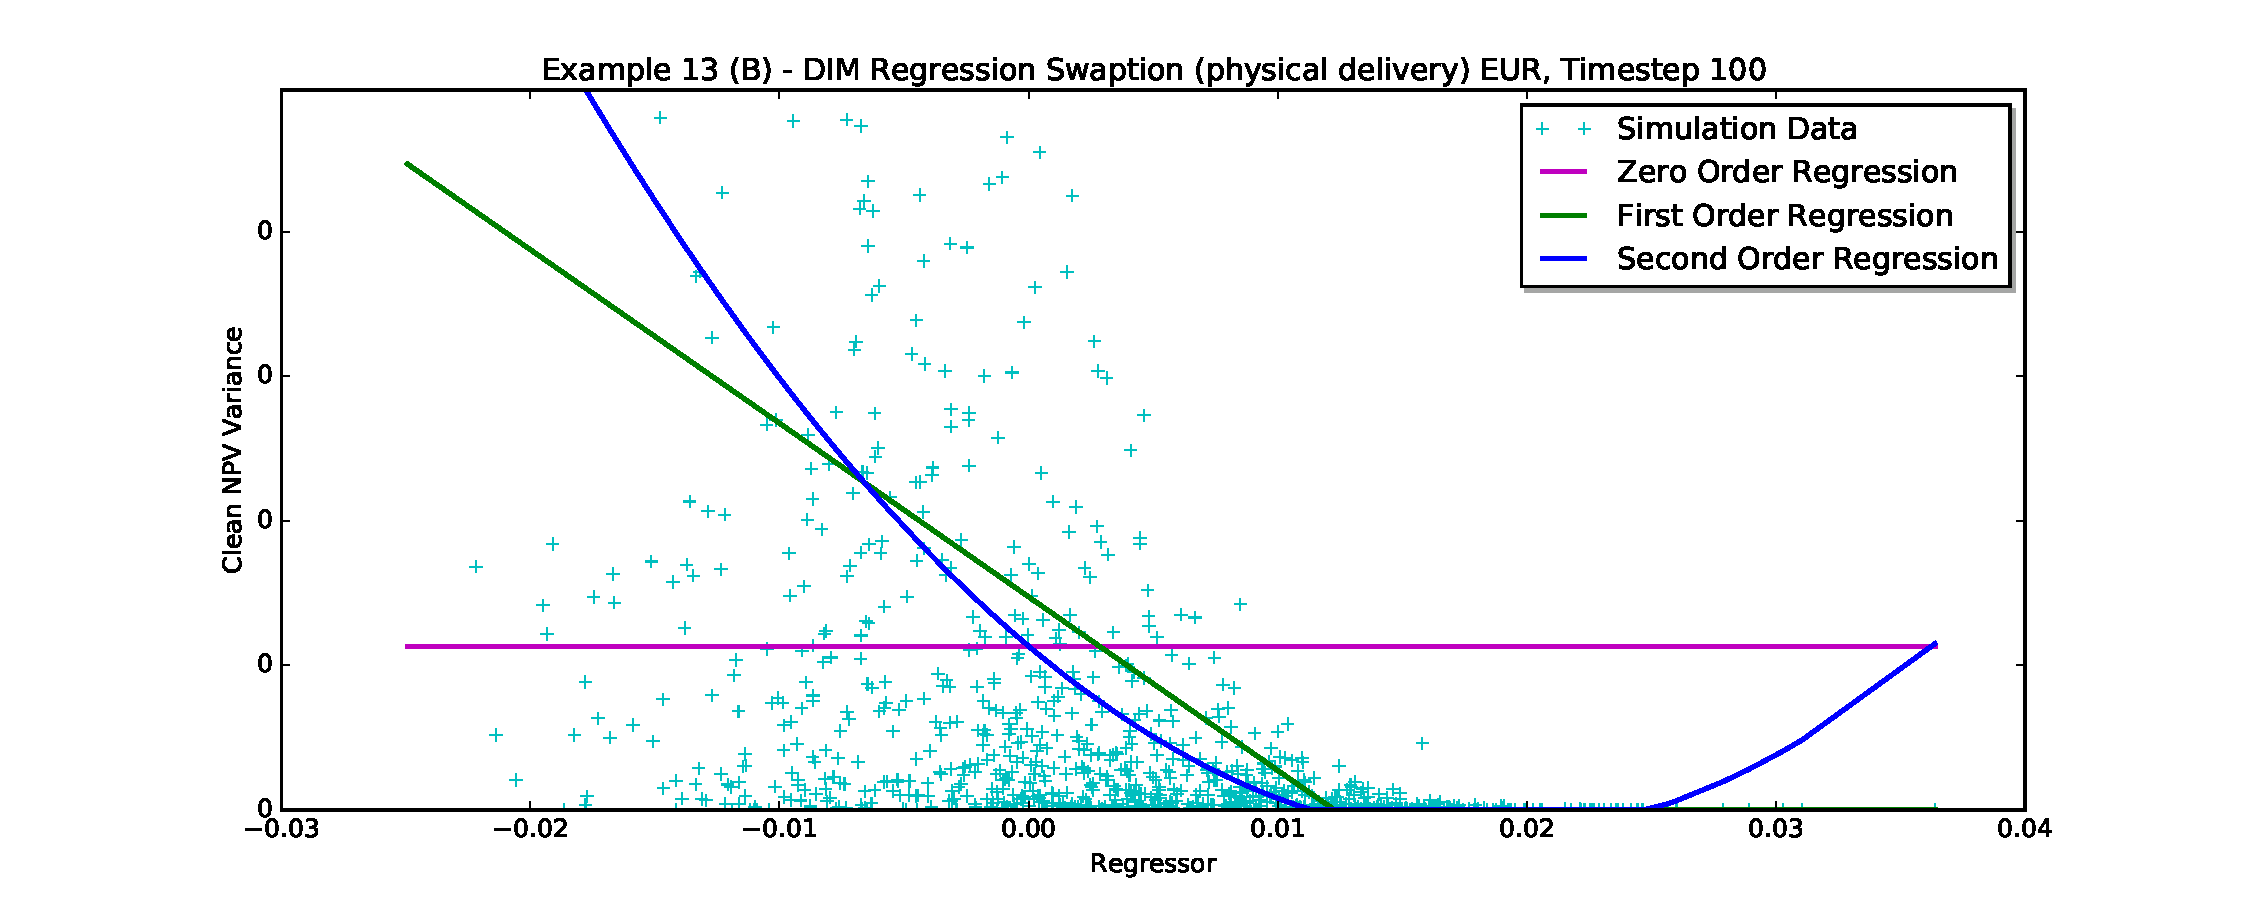
\includegraphics[scale=0.45]{mpl_dim_regression_B_swaption_eur_t100.pdf}
\end{center}
\caption{Regression snapshot at time step 100 (before expiry) for the EUR Swaption of Example 13 B.}
\label{fig_ex13b_regression}
\end{figure}

%--------------------------------------------------------
\subsection{Minimal Market Data Setup}
%--------------------------------------------------------

The example in folder {\tt Examples/Example\_14} demonstrates using a minimal market data setup in order to rerun the vanilla Swap exposure simulation shown in {\tt Examples/Example\_1}. The minimal market data uses single points per curve where possible.

%--------------------------------------------------------
\subsection{Sensitivity Analysis, Stress Testing and Parametric Value-at-Risk}\label{ex:sensitivity_stress}
%--------------------------------------------------------

The example in folder {\tt Examples/Example\_15} demonstrates the calculation of sensitivities and stress scenarios. The
portfolio used in this example consists of

\begin{itemize}
\item a vanilla swap in EUR
\item a cross currency swap EUR-USD
\item a resettable cross currency swap EUR-USD
\item a FX forward EUR-USD
\item a FX call option on USD/GBP % commented out?
\item a FX put option on USD/EUR
\item an European swaption
\item a Bermudan swaption 
\item a cap and a floor in USD
\item a cap and a floor in EUR
\item a fixed rate bond
\item a floating rate bond with floor
\item an Equity call option, put option and forward on S\&P500
\item an Equity call option, put option and forward on Lufthansa
\item a CPI Swap referencing UKRPI
\item a Year-on-Year inflation swap referencing EUHICPXT
\item a USD CDS.
\end{itemize}

The sensitivity configuration in {\tt sensitivity.xml} aims at computing the following sensitivities

\begin{itemize}
\item discount curve sensitivities in EUR, USD; GBP, CHF, JPY, on pillars 6M, 1Y, 2Y, 3Y, 5Y, 7Y, 10Y, 15Y, 20Y (absolute shift of 0.0001)
\item forward curve sensitivities for EUR-EURIBOR 6M and 3M indices, EUR-EONIA, USD-LIBOR 3M and 6M, GBP-LIBOR 3M and
  6M, CHF-LIBOR-6M and JPY-LIBOR-6M indices (absolute shift of 0.0001)
\item yield curve shifts for a bond benchmark curve in EUR (absolute shift of 0.0001)
\item FX spot sensitivities for USD, GBP, CHF, JPY against EUR as the base currency (relative shift of 0.01)
\item FX vegas for USDEUR, GBPEUR, JPYEUR volatility surfaces (relative shift of 0.01)
\item swaption vegas for the EUR surface on expiries 1Y, 5Y, 7Y, 10Y and underlying terms 1Y, 5Y, 10Y (relative shift of 0.01)
\item caplet vegas for EUR and USD on an expiry grid 1Y, 2Y, 3Y, 5Y, 7Y, 10Y and strikes 0.01, 0.02, 0.03, 0.04,
  0.05. (absolute shift of 0.0001)
\item credit curve sensitivities on tenors 6M, 1Y, 2Y, 5Y, 10Y (absolute shift of 0.0001).
\item Equity spots for S\&P500 and Lufthansa
\item Equity vegas for S\&P500 and Lufthansa at expiries 6M, 1Y, 2Y, 3Y, 5Y
\item Zero inflation curve deltas for UKRPI and EUHICPXT at tenors 6M, 1Y, 2Y, 3Y, 5Y, 7Y, 10Y, 15Y, 20Y
\item Year on year inflation curve deltas for EUHICPXT at tenors 6M, 1Y, 2Y, 3Y, 5Y, 7Y, 10Y, 15Y, 20Y
\end{itemize}

Furthermore, mixed second order derivatives (``cross gammas'') are computed for discount-discount, discount-forward and
forward-forward curves in EUR.

By definition the sensitivities are zero rate sensitivities and optionlet sensitivities, no par sensitivities are
provided. The sensitivity analysis produces three output files.

The first, {\tt scenario.csv}, contains the shift
direction ({\tt UP}, {\tt DOWN}, {\tt CROSS}), the base NPV, the scenario NPV and the difference of these two for each
trade and sensitivity key. For an overview over the possible scenario keys see \ref{sec:sensitivity}.

The second file, {\tt sensitivity.csv}, contains the shift size (in absolute terms always) and first (``Delta'') and second
(``Gamma'') order finite differences computed from the scenario results. Note that the Delta and Gamma results are pure
differences, i.e. they are not divided by the shift size.

The second file also contains second order mixed differences according to the specified cross gamma filter, along with the shift sizes for the two factors involved.

The stress scenario definition in {\tt stresstest.xml} defines two stress tests:

\begin{itemize}
\item {\tt parallel\_rates}: Rates are shifted in parallel by 0.01 (absolute). The EUR bond benchmark curve is shifted by
  increasing amounts 0.001, ..., 0.009 on the pillars 6M, ..., 20Y. FX Spots are shifted by 0.01 (relative), FX vols by
  0.1 (relative), swaption and cap floor vols by 0.0010 (absolute).
  Credit curves are not yet shifted.
\item {\tt twist}: The EUR bond benchmark curve is shifted by amounts -0.0050, -0.0040, -0.0030, -0.0020, 0.0020,
  0.0040, 0.0060, 0.0080, 0.0100 on pillars 6M, 1Y, 2Y, 3Y, 5Y, 7Y, 10Y, 15Y, 20Y.
\end{itemize}

The corresponding output file {\tt stresstest.csv} contains the base NPV, the NPV under the scenario shifts and the
difference of the two for each trade and scenario label.

%\todo[inline]{Update after CDS has been added to the example.}
\medskip
Finally, this example demonstrates a parametric VaR calculation based on the sensitivity and cross gamma output from the sensitivity analysis (deltas, vegas, gammas, cross gammas) and an external covariance matrix input. The result in {\tt var.csv} shows a breakdown by portfolio, risk class (All, Interest Rate, FX, Inflation, Equity, Credit) and risk type (All, Delta \& Gamma, Vega). The results shown are Delta Gamma Normal VaRs for the 95\% and 99\% quantile, the holding period is incorporated into the input covariances. Alternatively, one can choose a Monte Carlo VaR which means that the sensitivity based P\&L distribution is evaluated with MC simulation assuming normal respectively log-normal risk factor distribution. 
 
%--------------------------------------------------------
\subsection{Equity Derivatives Exposure}\label{ex:equityderivatives}
%--------------------------------------------------------

The example in folder {\tt Examples/Example\_16} demonstrates the computation of NPV, sensitivities, exposures and XVA for a portfolio 
of OTC equity derivatives. The portfolio used in this example consists of:

\begin{itemize}
	\item an equity call option denominated in EUR (``Luft'')
	\item an equity put option denominated in EUR (``Luft'')
	\item an equity forward denominated in EUR (``Luft'')
	\item an equity call option denominated in USD (``SP5'')
	\item an equity put option denominated in USD (``SP5'')
	\item an equity forward denominated in USD (``SP5'')
	\item an equity Swap in USD with return type  ``price'' (``SP5'')
	\item an equity Swap in USD with return type ``total'' (``SP5'')
\end{itemize}

The step-by-step procedure for running ORE is identical for equities as for other asset classes; the same market and 
portfolio data files are used to store the equity market data and trade details, respectively. For the exposure 
simulation, the calibration parameters for the equity risk factors can be set in the usual {\tt simulation.xml} file.

Looking at the MtM results in the output file {\tt npv.csv} we observe that put-call parity ($V_{Fwd} = V_{Call} - 
V_{Put}$) is observed as expected. Looking at Figure \ref{fig_eq_call} we observe that the Expected Exposure profile of 
the equity call option trade is relatively smooth over time, while for the equity forward trade the Expected Exposure 
tends to increase as we approach maturity. This behaviour is similar to what we observe in sections \ref{sec:fxfwd} 
and \ref{sec:fxoption}. 

\begin{figure}[h!]
	\begin{center}
		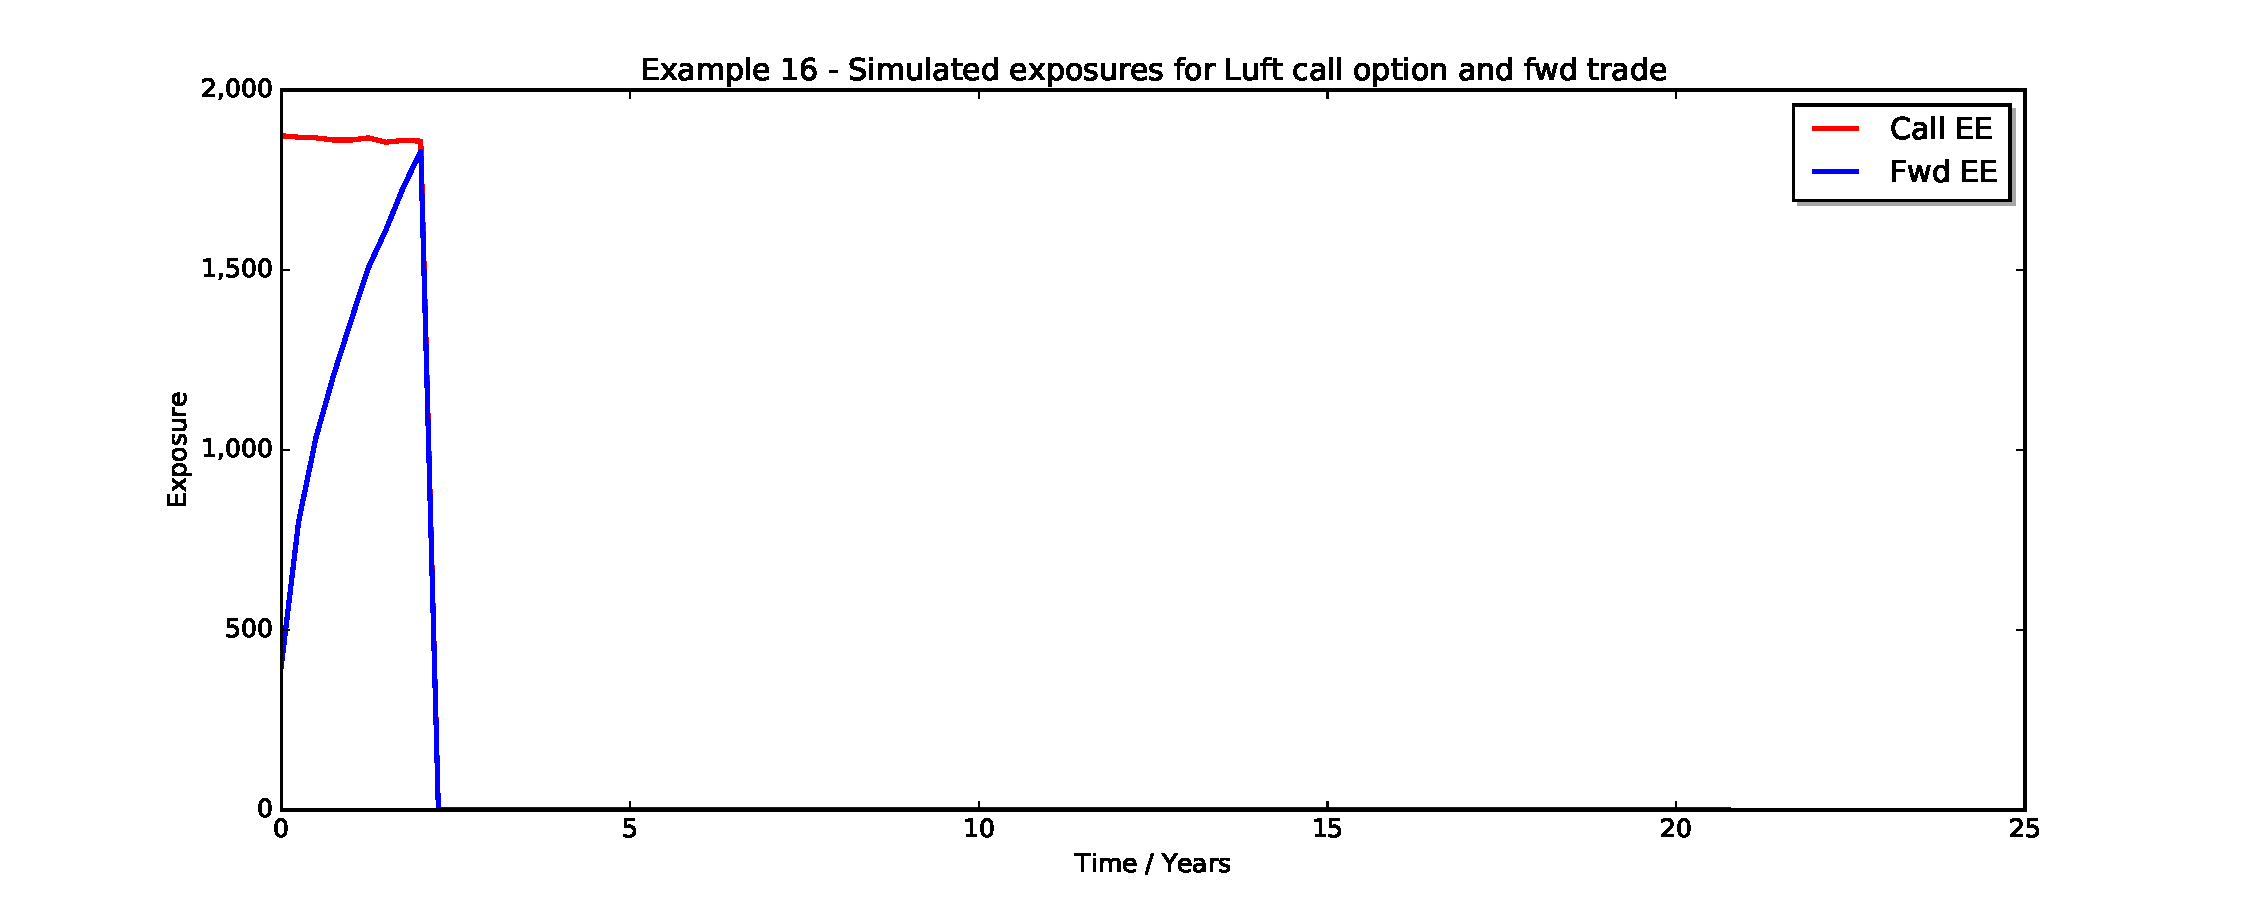
\includegraphics[scale=0.45]{mpl_eq_call.pdf}
	\end{center}
	\caption{Equity (``Luft'') call option and OTC forward exposure evolution, maturity in approximately 2.5 years. 
	Simulation with 
	10000 paths and quarterly time steps.}
	\label{fig_eq_call}
\end{figure}

%--------------------------------------------------------
\subsection{Inflation Swap Exposure under Dodgson-Kainth}% Example 17
\label{example:17}
%--------------------------------------------------------

The example portfolio in folder {\tt Examples/Example\_17} contains two CPI Swaps and one Year-on-Year Inflation Swap.
The terms of the three trades are as follows:

\begin{itemize}
\item CPI Swap 1: Exchanges on 2036-02-05 a fixed amount of 20m GBP for a 10m GBP notional inflated with UKRPI with base CPI 210
\item CPI Swap 2: Notional 10m GBP, maturity 2021-07-18, exchanging GBP Libor for GBP Libor 6M vs. $2\%$ x CPI-Factor (Act/Act), inflated with index UKRPI with base CPI 210
\item YOY Swap: Notional 10m EUR, maturity 2021-02-05, exchanging fixed coupons for EUHICPXT year-on-year inflation coupons
\item YOY Swap with capped/floored YOY leg: Notional 10m EUR, maturity 2021-02-05, exchanging fixed coupons for EUHICPXT year-on-year inflation coupons, YOY leg capped with 0.03 and floored with 0.005
\item YOY Swap with scheduled capped/floored YOY leg: Notional 10m EUR, maturity 2021-02-05, exchanging fixed coupons for EUHICPXT year-on-year inflation coupons, YOY leg capped with cap schedule and floored with floor schedule
\end{itemize}

The example generates cash flows, NPVs, exposure evolutions, XVAs, as well as two exposure graphs for CPI Swap 1 respectively the YOY Swap. For the YOY Swap and the both YOY Swaps with capped/floored YOY leg, the example generates their cash flows, NPVs, exposure evolutions, XVAs and sensitivities. Figure \ref{fig_cpi_swap} shows the CPI Swap exposure evolution.

\begin{figure}[h!]
	\begin{center}
		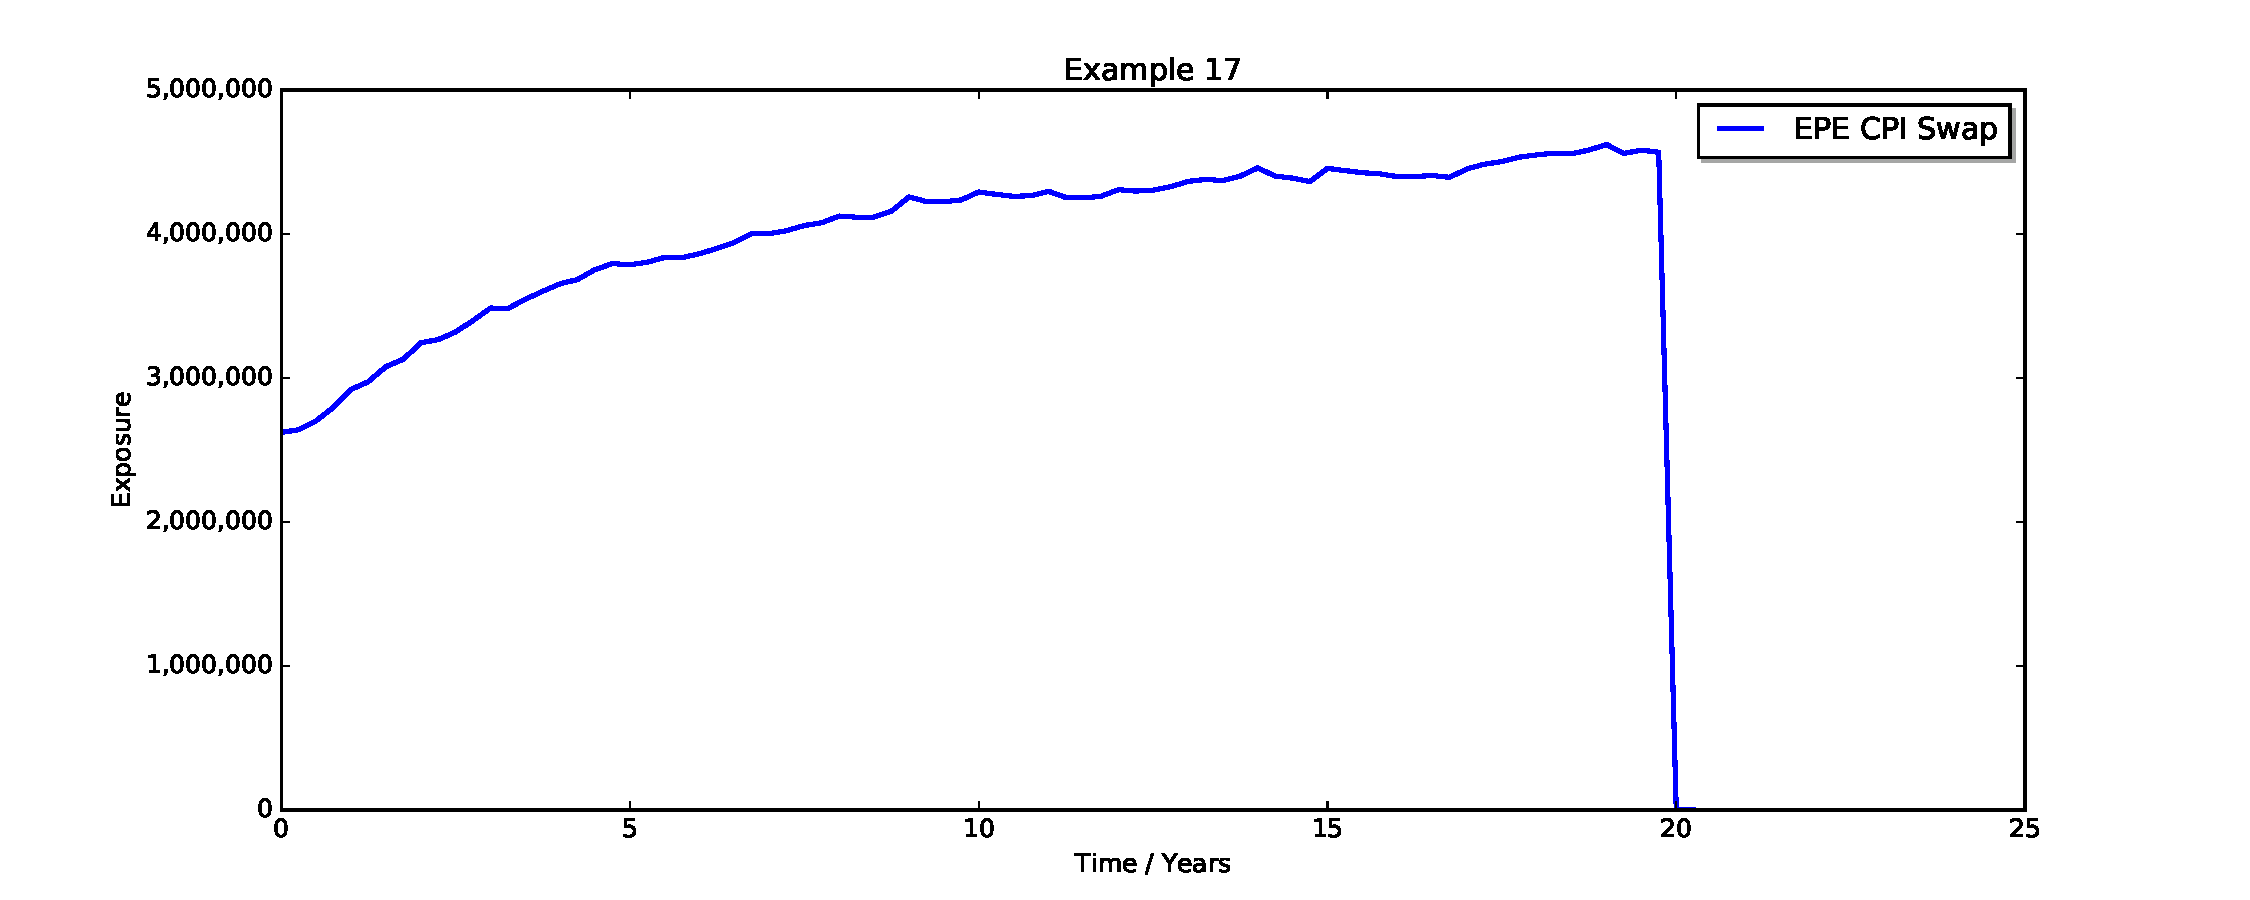
\includegraphics[scale=0.45]{mpl_cpi_swap.pdf}
	\end{center}
	\caption{CPI Swap 1 exposure evolution. Simulation with 1000 paths and quarterly time steps.}
	\label{fig_cpi_swap}
\end{figure}

Figure \ref{fig_yoy_swap} shows the evolution of the 5Y maturity Year-on-Year inflation swap for comparison. Note that the inflation simulation model (Dodgson-Kainth, see appendix \ref{sec:app_rfe}) yields the evolution of inflation indices and inflation zero bonds which allows spanning future inflation zero curves and the pricing of CPI swaps. To price Year-on-Year inflation Swaps under future scenarios, we imply Year-on-Year inflation curves from zero inflation curves\footnote{Currently we discard the required (small) convexity adjustment. This will be supplemented in a subsequent release.}. Note that for pricing Year-on-Year Swaps as of today we use a separate inflation curve bootstrapped from quoted Year-on-Year inflation Swaps.
 
\begin{figure}[h!]
	\begin{center}
		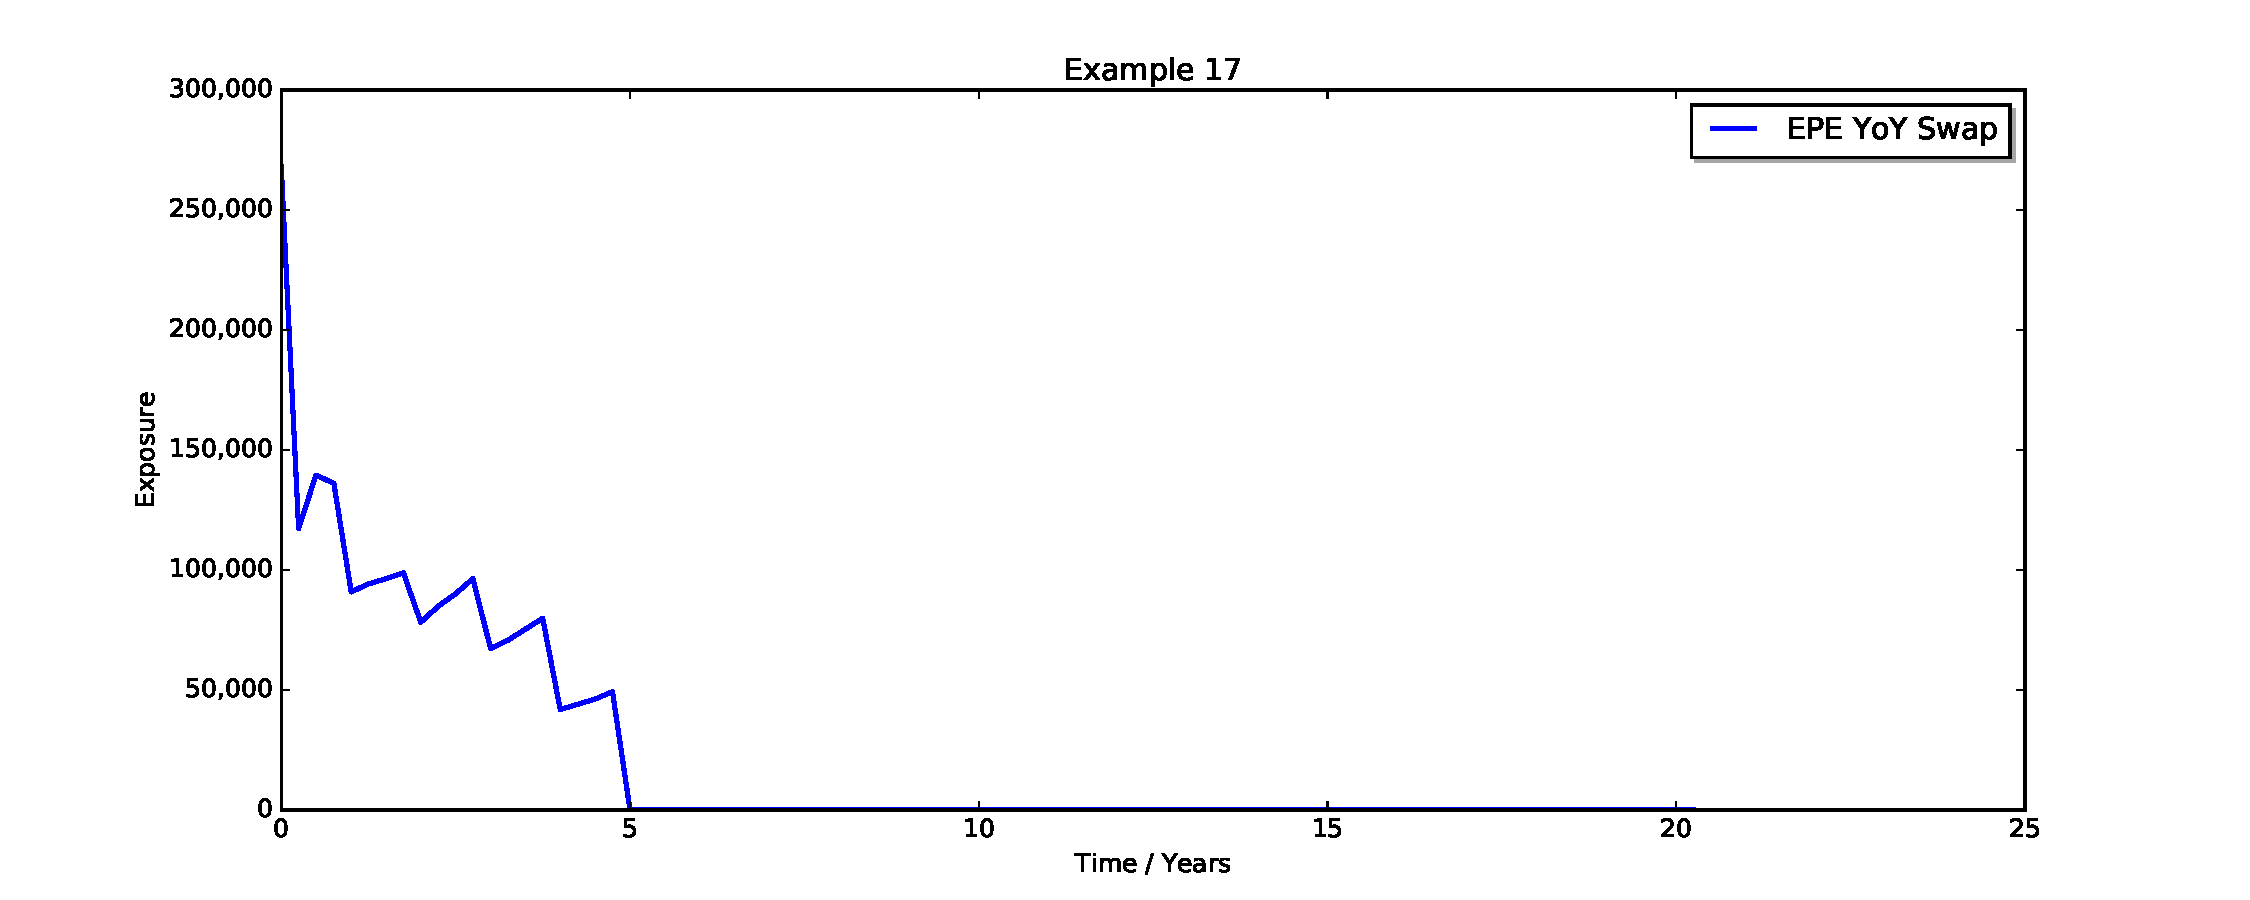
\includegraphics[scale=0.45]{mpl_yoy_swap.pdf}
	\end{center}
	\caption{Year-on-Year Inflation Swap exposure evolution. Simulation with 1000 paths and quarterly time steps.}
	\label{fig_yoy_swap}
\end{figure}

%--------------------------------------------------------
\subsection{Bonds and Amortisation Structures}% Example 18
%--------------------------------------------------------

The example in folder {\tt Examples/Example\_18} computes NPVs and cash flow projections for a vanilla bond portfolio
consisting of a range of bond products, in particular demonstrating amortisation features:
\begin{itemize}
\item fixed rate bond
\item floating rate bond linked to Euribor 6M
\item bond switching from fixed to floating
\item bond with 'fixed amount' amortisation
\item bond with percentage amortisation relative to the initial notional
\item bond with percentage amortisation relative to the previous notional
\item bond with fixed annuity amortisation
\item bond with floating annuity amortisation (this example needs QuantLib 1.10 or higher to work, in particular the amount() method in the Coupon class needs to be virtual)
\item bond with fixed amount amortisation followed by percentage amortisation relative to previous notional
\end{itemize}

After running the example, the results of the computation can be found in the output files {\tt npv.csv} and {\tt
  flows.csv}, respectively.

\medskip
Note that the amortisation features used here are linked to the LegData structure, hence not limited to the Bond instrument, see section \ref{ss:amortisationdata}.

%--------------------------------------------------------
\subsection{Swaption Pricing with Smile}% Example 19
%--------------------------------------------------------

This example in folder {\tt Examples/Example\_19} demonstrates European Swaption pricing with and without smile. Calling

\medskip
\centerline{\tt python run.py}

\medskip
will launch two ORE runs using config files {\tt ore\_flat.xml} and {\tt ore\_smile.xml}, respectively. The only difference in these is referencing alternative market configurations {\tt todaymarket\_flat.xml} and {\tt todaysmarket\_smile.xml} using an ATM Swaption volatility matrix and a Swaption cube, respectively. NPV results are written to {\tt npv\_flat.cvs} and {\tt npv\_smile.csv}.

%--------------------------------------------------------
\subsection{Credit Default Swap Pricing}% Example 20
%--------------------------------------------------------

This example in folder {\tt Examples/Example\_20} demonstrates Credit Default Swap pricing via ORE. Calling

\medskip
\centerline{\tt python run.py}

\medskip
will launch a single ORE run to process a single name CDS example and to generate NPV and cash flows in the usual result files. 

\medskip
CDS can be included in sensitivity analysis and stress testing. Exposure simulation for credit derivatives will follow in the next ORE release.

%--------------------------------------------------------
\subsection{CMS and CMS Cap/Floor Pricing}% Example 21
%--------------------------------------------------------

This example in folder {\tt Examples/Example\_21} demonstrates the pricing of CMS and CMS Cap/Floor using a portfolio consisting of a CMS Swap (CMS leg vs. fixed leg) and a CMS Cap. Calling

\medskip
\centerline{\tt python run.py}

\medskip
will launch a single ORE run to process the portfolio and generate NPV and cash flows in the usual result files. 

\medskip
CMS structures can be included in sensitivity analysis, stress testing and exposure simulation. 

%--------------------------------------------------------
\subsection{Option Sensitivity Analysis with Smile}% Example 22
%--------------------------------------------------------

The example in folder {\tt Examples/Example\_22} demonstrates the current state of sensitivity calculation for European options where the volatility surface has a smile. 

\medskip
The portfolio used in this example consists of
\begin{itemize}
	\item an equity call option denominated in USD (``SP5'')
	\item an equity put option denominated in USD (``SP5'')
	\item a receiver swaption in EUR
	\item an FX call option on EUR/USD
\end{itemize}

\medskip
Refer to appendix \ref{sec:app_sensi} for the current status of sensitivity implementation with smile. In this example the setup is as follows
\begin{itemize}
\item today's market is configured with volatility smile for all three products above
\item simulation market has two configurations, to simulate ``ATM only'' or the ``full surface''; ``ATM only'' means that only ATM volatilities are to be simulated and shifts to ATM vols are propagated to the respective smile section (see appendix \ref{sec:app_sensi});  
\item the sensitivity analysis has two corresponding configurations as well, ``ATM only'' and ``full surface''; note that the ``full surface'' configuration leads to explicit sensitivities by strike only in the case of Swaption volatilities, for FX and Equity volatilities only ATM sensitivity can be specified at the moment and sensitivity output is currently aggregated to the ATM bucket (to be extended in subsequent releases).
\end{itemize}

The respective output files end with ``{\tt\_fullSurface.csv}'' respectively ``{\tt\_atmOnly.csv}''.

%ORE supports two methods of simulating equity volatility smile. The first method simulates the entire surface using specific moneyness levels configured in simulation.xml. The second method simulates only the ATM equity volatilities, the other strikes are shifted relative to this new ATM using the $t_{0}$ smile.  This example compares both methods using the same sensitivity configuration as in {\tt Examples/Example\_15}. For the first method {\tt simulation\_fullSurface.xml} is used and all output files are appended with ``\_fullSurface'', for the second method {\tt simulation\_atmOnly.xml} is used and all output files are appended with ``\_atmOnly''.


%--------------------------------------------------------
\subsection{FRA and Average OIS Exposure}% Example 23
%--------------------------------------------------------

This example in folder {\tt Examples/Example\_23} demonstrates pricing, cash flow projection and exposure simulation for two additional products
\begin{itemize}
\item Forward Rate Agreements
\item Averaging Overnight Index Swaps
\end{itemize}
using a minimal portfolio of four trades, one FRA and three OIS. The essential results are in {\tt npv.csv}, {\tt flows.csv} and 
four {\tt exposure\_trade\_*.csv} files.

%--------------------------------------------------------
\subsection{Commodity Derivatives, Pricing, Sensitivity, Exposure}% Example 24
\label{example:24}
%--------------------------------------------------------

Calling

\medskip
\centerline{\tt python run.py}

\medskip
in folder {\tt Examples/Example\_24} will launch two ORE runs. The first one determined by {\tt ore.xml} demonstrates pricing and sensitivity analysis for
\begin{itemize}
\item Commodity Forwards
\item European Commodity Options
\end{itemize}
using a minimal portfolio of four forwards and two options referencing WTI and Gold. 
The essential results are in {\tt npv.csv} and {\tt sensitivity.csv}.

The second run determined by {\tt ore\_wti.xml} demonstrates Commodity exposure simulation for a portfolio including a
\begin{itemize}
\item Commodity Forward
\item Commodity Swap
\item European Commodity Option
\item Commodity Average Price Option
\item Commodity Swaption
\end{itemize}
with the usual results, exposure reports and graphs. 

%--------------------------------------------------------
\subsection{CMS Spread with (Digital) Cap/Floor}% Example 25
\label{example:25}
%--------------------------------------------------------

The example in folder {\tt Examples/Example\_25}  demonstrates pricing, sensitivity analysis 
and exposure simulation for 
\begin{itemize}
\item Capped/Floored CMS Spreads
\item CMS Spreads with Digital Caps/Floors
\end{itemize}

The example can be run with

\medskip
\centerline{\tt python run.py}

\medskip
and results are in {\tt npv.csv}, {\tt sensitivity.csv}, {\tt exposure\_*.csv} 
and the exposure graphs in {\tt mpl\_cmsspread.pdf}.

%--------------------------------------------------------
\subsection{Bootstrap Consistency}% Example 26
%--------------------------------------------------------

The example in folder {\tt Examples/Example\_26} confirms that bootstrapped curves 
correctly reprice the bootstrap instruments (FRAs, Interest Rate Swaps, FX Forwards, Cross
Currency Basis Swaps) using three pricing setups with
\begin{itemize}
\item EUR collateral discounting (configuration xois\_eur)
\item USD collateral discounting (configuration xois\_usd)
\item in-currency OIS discounting (configuration collateral\_inccy)
\end{itemize}
all defined in {\tt Examples/Input/todaysmarket.xml}.

\medskip
The required portfolio files need to be generated from market data and conventions in
{\tt Examples/Input} and trade templates in 
{\tt Examples/Example\_26/Helpers}, calling

\medskip
\centerline{\tt python TradeGenerator.py}

\medskip
This will place three portfolio files {\tt *\_portfolio.xml} in the input folder.
Thereafter, the three consistency checks can be run calling

\medskip
\centerline{\tt python run.py}

\medskip
Results are in three files {\tt *\_npv.csv} and should show zero NPVs for all benchmark instruments.

%--------------------------------------------------------
\subsection{BMA Basis Swap}% Example 27
\label{example:27}
%--------------------------------------------------------

The example in folder {\tt Examples/Example\_27} demonstrates pricing 
and sensitivity analysis for a series of USD Libor 3M vs. Averaged BMA (SIFMA) 
Swaps that correspond to the instruments used to bootstrap the BMA curve. 

The example can be run with

\medskip
\centerline{\tt python run.py}

\medskip
and results are in {\tt npv.csv} and {\tt sensitivity.csv}.

%--------------------------------------------------------
\subsection{Discount Ratio Curves}% Example 28
\label{example:28}
%--------------------------------------------------------

The example in folder {\tt Examples/Example\_28} shows how to use a yield curve 
built from a DiscountRatio segment. 
In particular, it builds a GBP collateralized in EUR discount curve by referencing 
three other discount curves:
\begin{itemize}
\item a GBP collateralised in USD curve
\item a EUR collateralised in USD curve
\item a EUR OIS curve i.e. a EUR collateralised in EUR curve
\end{itemize}

The implicit assumption in building the curve this way is that EUR/GBP FX 
forwards collateralised in EUR have the same fair market rate as EUR/GBP 
FX forwards collateralised in USD. This assumption is illustrated in the 
example by the NPV of the two forward instruments in the portfolio returning 
exactly 0 under both discounting regimes i.e. under USD collateralization with 
direct curve building and under EUR collateralization with the discount ratio 
modified ``GBP-IN-EUR'' curve.

Also, in this example, an assumption is made that there are no direct GBP/EUR FX 
forward or cross currency quotes available which in general is false. The example 
s merely for illustration.

Both collateralizaton scenarios can be run calling {\tt python run.py}.

%--------------------------------------------------------
\subsection{Curve Building using Fixed vs. Float Cross Currency Helpers}% Example 29
\label{example:29}
%--------------------------------------------------------

The example in folder {\tt Examples/Example\_29} demonstrates using fixed vs. float 
cross currency swap helpers. In particular, it builds a TRY collateralised in USD 
discount curve using TRY annual fixed vs USD 3M Libor swap quotes.

The portfolio contains an at-market fixed vs. float cross currency swap that is 
included in the curve building. The NPV of this swap should be zero when the example is run,
using {\tt python run.py} or ``directly'' calling {\tt ore[.exe] ore.xml}.

%--------------------------------------------------------
\subsection{USD-Prime Curve Building via Prime-LIBOR Basis Swap}% Example 30
\label{example:30}
%--------------------------------------------------------

The example in folder {\tt Examples/Example\_30} demonstrates the implementation of the USD-Prime index in the ORE.
The USD-Prime yield curve is built from USD-Prime vs USD 3M Libor basis swap quotes.
The portfolio consists of two fair basis swaps (NPVs equal to 0):
\begin{itemize}
\item US Dollar Prime Rate vs 3 Month LIBOR
\item US Dollar 3 Month LIBOR vs Fed Funds + 0.027
\end{itemize}

In particular, it is confirmed that the bootstrapped curves USD-FedFunds and USD-Prime follow
the 3\% rule observed on the market: {\tt U.S. Prime Rate = (The Fed Funds Target Rate + 3\%)}.
(See \url{http://www.fedprimerate.com/}.)

Running ORE in directory {\tt Examples/Example\_30} with {\tt python run.py }
yields the USD-Prime curve in {\tt Examples/Example\_30/Output/curves.csv.}

%--------------------------------------------------------
\subsection{Exposure Simulation using a Close-Out Grid}% Example 31
\label{example:31}
%--------------------------------------------------------

In the previous examples we have used a ``lagged'' approach, described at the end of appendix \ref{sec:app_collateral}, to take the Margin Period of Risk into account in exposure modelling. This has the disadvantage in ORE that we need to use equally-spaced time grids with time steps that match the MPoR, e.g. 2W, out to final portfolio maturity. 

In this example we demonstrate an alternative approach supported by ORE since release 6. In this approach we use two nested grids: The (almost) arbitrary main simulation grid is used to compute ``default values'' which feed into the collateral balance $C(t)$ filtered by MTA and Threshold etc; an auxiliary ``close-out'' grid, offset from the main grid by the MPoR, is used to compute the delayed close-out values $V(t)$ associated with time default time $t$. The difference between $V(t)$ and $C(t)$ causes a residual exposure $[V(t)-C(t)]^+$ even if minimum transfer amounts and thresholds are zero.

The close-out date value can be computed in two ways in ORE
\begin{itemize}
\item as of default date, by just evolving the market from default date to close-out date
   (``sticky date''), or 
\item  as of close-out date, by evolving both valuation date and market over the 
   close-out period (``actual date''), i.e., the portfolio ages and cash flows might occur
   in the close-out period causing spikes in the evolution of exposures. 
\end{itemize}

We are reusing one case from Example 10 here, perfect CSA with zero threshold and
minimum transfer amount, so that the remaining exposure is solely due to the MPoR
effect. The portfolio consists of a single at-the-money Swap in GBP. 
The relevant configuration changes that trigger this modelling are in the Parameters section of {\tt simulation.xml} as shown in Listing \ref{lst:close_out_grid}

\begin{listing}[H]
\begin{minted}[fontsize=\footnotesize]{xml}
  <Parameters>
    <Grid> ... </Grid>
    <Calendar> ... </Calendar>
    <Sequence> ... </Sequence>
    <Scenario> ... </Scenario>
    <Seed> ... </Seed>
    <Samples> ... </Samples>
    <CloseOutLag> 2W </CloseOutLag>
    <MporMode> StickyDate </MporMode><!-- Alternative: ActualDate -->
  </Parameters>
\end{minted}
\caption{Close-out grid specification}
\label{lst:close_out_grid}
\end{listing}

and moreover in the XVA analytics section of {\tt ore\_mpor.xml} as shown in Listing \ref{lst:calctype_nolag}.

\begin{listing}[H]
\begin{minted}[fontsize=\footnotesize]{xml}
  <Analytic type="xva">
    ...
    <Parameter name="calculationType"> NoLag </Parameter>
    ...
  </Parameters>
\end{minted}
\caption{Close-out grid specification}
\label{lst:calctype_nolag}
\end{listing}

Run as usual calling {\tt python run.py}.

%--------------------------------------------------------------------
\subsection{Inflation Swap Exposure under Jarrow-Yildrim}% Example 32
\label{example:32}
%--------------------------------------------------------------------

The example here is similar to that in Section \ref{example:17} in that we are generating exposures for inflation swaps. The example in Section \ref{example:17} uses the Dodgson-Kainth model whereas this example uses the Jarrow-Yildrim model. The valuation date is 5 Oct 2020 and the portfolio contains four spot starting inflation swaps:

\begin{itemize}
\item trade\_01: 20Y standard UKRPI ZCIIS struck at the fair market rate of 3.1925\% giving an NPV of 0.0. 
\item trade\_02: 20Y standard EUHICPXT ZCIIS struck at the fair market rate of 1.16875\% giving an NPV of 0.0.
\item trade\_03: 20Y year on year EUHICPXT swap.
\item trade\_04: 20Y year on year UKRPI swap.
\end{itemize}

The example generates cash flows, NPVs, exposure evolutions and XVAs.

%--------------------------------------------------------------------
\subsection{CDS Exposure Simulation}% Example 33
\label{example:33}
%--------------------------------------------------------------------

The example in folder {\tt Examples/Example\_33} is the credit variant of the example in
\ref{sec:example1}. Running ORE in directory {\tt Examples/Example\_33} with

\medskip
\centerline{\tt python run.py } 
\medskip

yields the exposure evolution in 

\medskip
\centerline{\tt Examples/Example\_33/Output/*.pdf } 
\medskip

and shown in figure \ref{fig_33}. 
\begin{figure}[h!]
\begin{center}
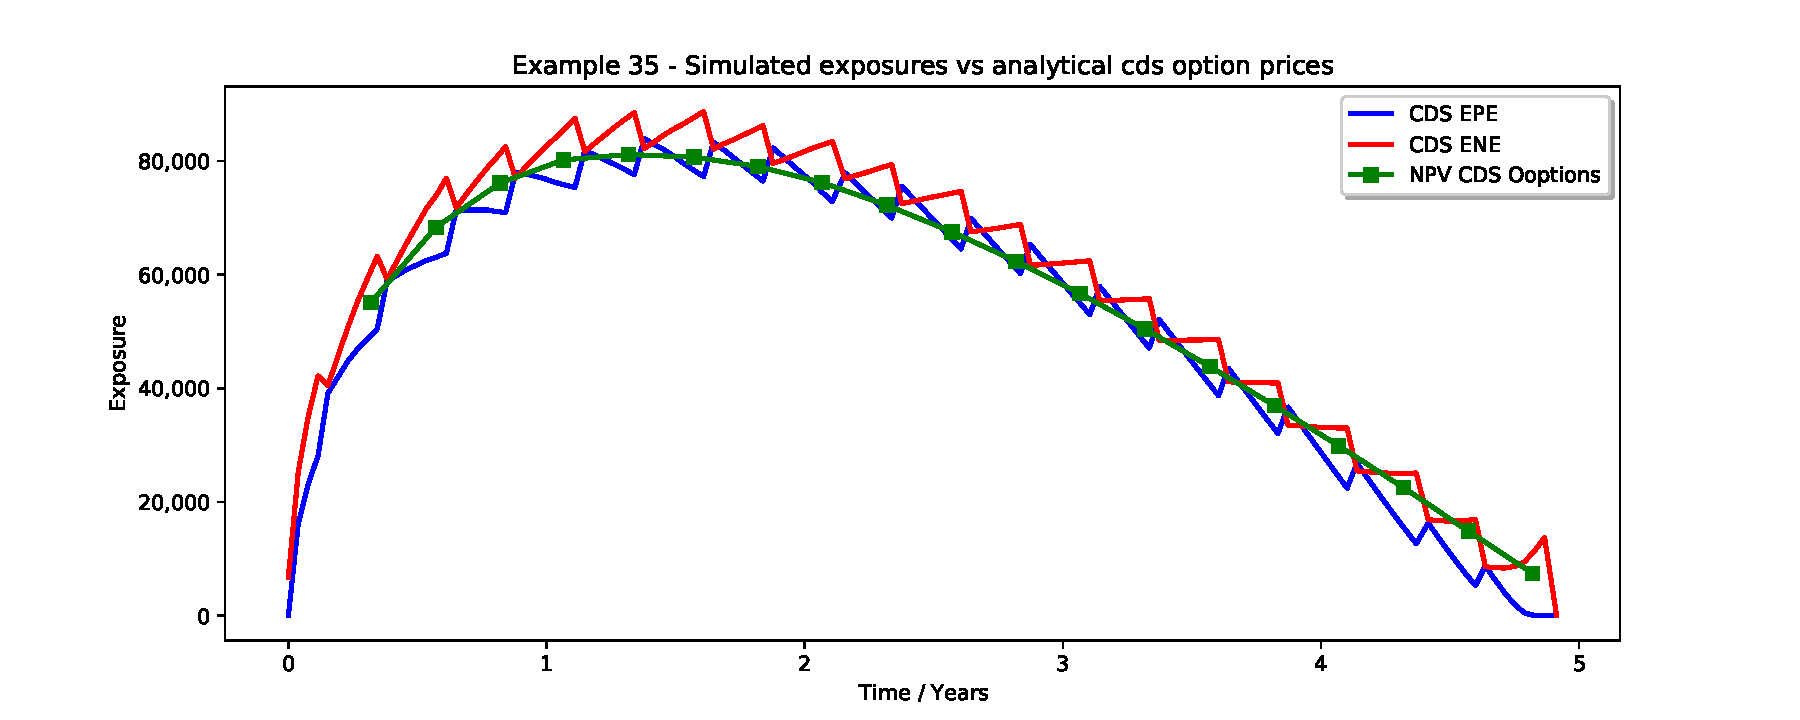
\includegraphics[scale=0.45]{mpl_cds_33_2w_10k.pdf}
\end{center}
\caption{Credit Default Swap expected exposure in a flat market environment from both parties' perspectives. The symbols are CDS Option prices. The simulation was run with bi-weekly time steps and 10,000 Monte Carlo samples to demonstrate the convergence of EPE and ENE profiles. A similar
outcome can be obtained more quickly with 5,000 samples on a monthly time grid which is the default setting of Example\_33. }
\label{fig_33}
\end{figure}
Both CDS simulation and CDS Option pricing are run with calls to the ORE executable, essentially 

\medskip
\centerline{\tt ore[.exe] ore.xml} 

\centerline{\tt ore[.exe] ore\_cds\_option.xml} 
\medskip

which are wrapped into the script {\tt Examples/Example\_33/run.py} provided with the ORE release.

This example demonstrates credit simulation using the LGM model and the calculation of Wrong Way Risk due to credit
correlation between the underlying entity of the CDS and the counterparty of the CDS trade via dynamic credit.
Positive correlation between the two names weakens the protection of the CDS whilst
negative correlation strengthens the protection.

The following table lists the XVA result from the example at different levels of correlation.


\begin{table}[hbt]
\scriptsize
\begin{center}
\begin{tabular}{|r|l|r|r|r|r|}
\hline
Correlation & NettingSetId & CVA & DVA & FBA & FCA \\
\hline
-100\%  &  CPTY\_B  &  -2,638  &  2,906  &  486  &  -1,057 \\
 -90\%  &  CPTY\_B  &  -2,204  &  2,906  &  488  &  -1,053 \\
 -50\%  &  CPTY\_B  &    -485  &  2,906  &  493  &  -1,040 \\
 -40\%  &  CPTY\_B  &     -60  &  2,906  &  495  &  -1,037 \\
 -30\%  &  CPTY\_B  &     363  &  2,906  &  496  &  -1,033 \\
 -20\%  &  CPTY\_B  &     784  &  2,906  &  498  &  -1,030 \\
 -10\%  &  CPTY\_B  &   1,204  &  2,906  &  500  &  -1,027 \\
   0\%  &  CPTY\_B  &   1,621  &  2,906  &  501  &  -1,023 \\
  10\%  &  CPTY\_B  &   2,036  &  2,906  &  503  &  -1,020 \\
  20\%  &  CPTY\_B  &   2,450  &  2,906  &  504  &  -1,017 \\
  30\%  &  CPTY\_B  &   2,861  &  2,906  &  506  &  -1,013 \\
  40\%  &  CPTY\_B  &   3,271  &  2,906  &  507  &  -1,010 \\
  50\%  &  CPTY\_B  &   3,679  &  2,906  &  509  &  -1,017 \\
  90\%  &  CPTY\_B  &   5,290  &  2,906  &  515  &    -994 \\
 100\%  &  CPTY\_B  &   5,689  &  2,906  &  517  &    -991 \\
\hline
\end{tabular}
\caption{CDS XVA results with LGM model}
\end{center}
\end{table}

%--------------------------------------------------------------------
\subsection{Wrong Way Risk}% Example 34
\label{example:34}
%--------------------------------------------------------------------

The example in folder {\tt Examples/Example\_34} is an extension of the example in
\ref{sec:example1} with dynamic credit and IR-CR correlation. As we are paying
float, negative correlation implies that we pay more when the counterparty's credit
worsens, leading to a surge of CVA.

The following table lists the XVA result from the example at different levels of correlation.

\begin{table}[hbt]
\scriptsize
\begin{center}
\begin{tabular}{|r|l|r|r|r|r|}
\hline
Correlation & NettingSetId & CVA & DVA & FBA & FCA \\
\hline
 -30\%  &  CPTY\_A  & 105,146  &  68,061  &  31,519  &  -4,127 \\
 -20\%  &  CPTY\_A  &  88,442  &  68,061  &  30,976  &  -4,219 \\
 -10\%  &  CPTY\_A  &  71,059  &  68,061  &  30,439  &  -4,314 \\
   0\%  &  CPTY\_A  &  52,983  &  68,061  &  29,909  &  -4,411 \\
  10\%  &  CPTY\_A  &  34,199  &  68,061  &  29,386  &  -4,511 \\
  20\%  &  CPTY\_A  &  14,691  &  68,061  &  28,869  &  -4,614 \\
  30\%  &  CPTY\_A  &  -5,554  &  68,061  &  28,360  &  -4,719 \\
\hline
\end{tabular}
\caption{IR Swap XVA results with LGM model}
\end{center}
\end{table}

%--------------------------------------------------------------------
\subsection{Flip View}% Example 35
\label{example:35}
%--------------------------------------------------------------------

The example in folder {\tt Examples/Example\_35} demonstrates how ORE can be used to quickly switch perspectives in XVA calculations with minimal changes in the {\tt ore.xml} file only. In particular it does not involve manipulating the portfolio input or the netting set.

%--------------------------------------------------------------------
\subsection{Choice of Measure}% Example 36
\label{example:36}
%--------------------------------------------------------------------

The example in folder {\tt Examples/Example\_36} illustrates the effect of measure changes on simulated expected and peak exposures. For that purpose we reuse Example 1 (un-collateralized vanilla swap exposure) and run the simulation three times with different risk-neutral measures,
\begin{itemize}
\item in the LGM measure as in Example 1 (note {\tt <Measure>LGM</Measure>} in {\tt simulation\_lgm.xml}, this is the default also if the Measure tag is omitted)  
\item in the more common Bank Account measure (note {\tt <Measure>BA</Measure>} in {\tt simulation\_ba.xml})  
\item in the T-Forward measure with horizon T=20 at the Swap maturity (note {\tt <Measure>LGM</Measure>}  and {\tt <ShiftHorizon>20.0</ShiftHorizon>} in {\tt simulation\_fwd.xml})
\end{itemize}

The results are summarized in the exposure evolution graphs in figure \ref{fig:36}. As expected, the expected exposures evolutions match across measures, as these are expected discounted NPVs and hence measure independent.
However, peak exposures are dependent on the measure choice as confirmed graphically here. Many more measures are accessible with ORE, by way of varying the T-Forward horizon which was chosen arbitrarily here to match the Swap's maturity.

\begin{figure}[h!]
\begin{center}
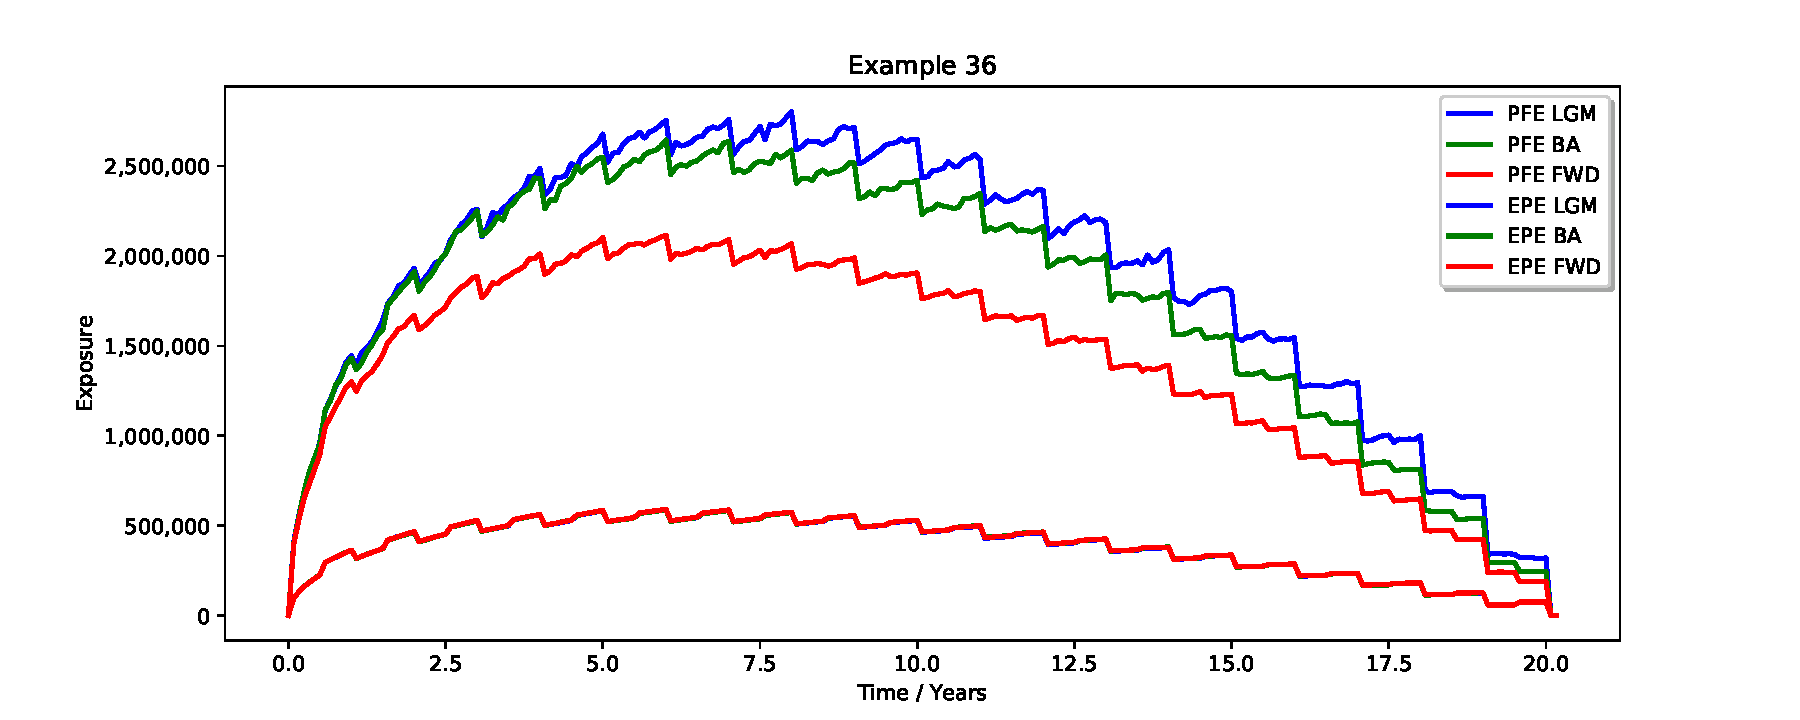
\includegraphics[scale=0.45]{mpl_exposures_measures.pdf}
\end{center}
\caption{Evolution of expected exposures (EPE) and peak exposures (PFE at the 95\% quantile) in three measures, LGM, Bank Account, T-Forward with T=20, with 10k Monte Carlo samples.}
\label{fig:36}
\end{figure}

%--------------------------------------------------------------------
\subsection{Multifactor Hull-White Scenario Generation}% Example 37
\label{example:37}
%--------------------------------------------------------------------

The example in folder {\tt Examples/Example\_37} illustrates the scenario generation under a Hull-White multifactor
model. The model is driven by two independent Brownian motions and has four states. The diffusion matrix sigma is
therefore 2 x 4. The reversion matrix is a 4 x 4 diagonal matrix and entered as an array. Both diffusion and reversion
are constant in time. Their values are not calibrated to the option market, but hardcoded in simulation.xml.

The values for the diffusion and reversion matrices were fitted to the first two principal components of a
(hypothetical) analyis of absolute rate curve movements. These input principal components can be found in
inputeigenvectors.csv in the input folder. The tenor is given in years, and the two components are given as column
vectors, see table \ref{tab:ex37_1}.

\begin{table}[hbt]
\begin{center}
\begin{tabular}{r|r|r}
tenor & eigenvector 1  & eigenvector 2   \\
\hline      
1     & 0.353553390593 & -0.537955502871 \\
2     & 0.353553390593 & -0.374924478795 \\
3     & 0.353553390593 & -0.252916811525 \\
5     & 0.353553390593 & -0.087587539893 \\
10    & 0.353553390593 & 0.12267800393   \\
15    & 0.353553390593 & 0.240659435416  \\
20    & 0.353553390593 & 0.339148675322  \\
30    & 0.353553390593 & 0.552478951238
\end{tabular}
\caption{Input principal components}
\label{tab:ex37_1}
\end{center}
\end{table}

The first eigenvector represent perfectly parallel movements. The second eigenvector represent a rotation around the 7y
point of the curve. Furthermore we prescribe an annual volatility of 0.0070 for the first components and 0.0030 for the
second one. The values can be compared to normal (bp) volatilities.

We follow \cite{Andersen_Piterbarg_2010} chapter 12.1.5 ``Multi-Factor Statistical Gaussian Model'' to calibrate the
diffusion and reversion matrices to the prescribed components and volatilities. We do not detail the procedure here and
refer the interested reader to the given reference.

The example generates a single monte carlo path with 5000 daily steps and outputs the generated scenarios in
scenariodump.csv. The python script pca.py performs a principal component analysis on this output. The model implied
eigenvalues are given in table \ref{tab:ex37_2}.

\begin{table}[hbt]
\begin{center}
\begin{tabular}{r|r}
number & value                  \\
\hline      
1      & 4.9144936649319346e-05 \\
2      & 8.846877641067412e-06  \\
3      & 5.82566039467854e-10   \\
4      & 2.1298948225571415e-10 \\
5      & 9.254913949332787e-11  \\
6      & 1.0861256211767673e-11 \\
7      & 8.478795662698618e-14  \\
8      & 9.74468069377584e-13   \\
\end{tabular}
\caption{Input principal components}
\label{tab:ex37_2}
\end{center}
\end{table}

Only the first two values are relevant, the following are all close to zero. The square root of the first two
eigenvalues is given in table \ref{tab:ex37_3}.

\begin{table}[hbt]
\begin{center}
\begin{tabular}{r|r}
number & sqrt(value)                \\
\hline      
1      & 0.007010344973631422       \\
2      & 0.0029743701250966414      \\
\end{tabular}
\caption{Input principal components}
\label{tab:ex37_3}
\end{center}
\end{table}

matching the prescribed input values of 0.0070 and 0.0030 quite well. The correpsonding eigenvectors are given in etable
\ref{tab:ex37_4}.

\begin{table}[hbt]
\begin{center}
\begin{tabular}{r|r|r}
tenor & eigenvector 1       & eigenvector 2       \\
\hline      
1     & 0.34688826736335926 & 0.5441204725042812  \\
2     & 0.3489303472083185  & 0.380259707350115   \\
3     & 0.350362134519783   & 0.2581408080614405  \\
5     & 0.3523983915961889  & 0.09230899007104967 \\
10    & 0.3550169593982022  & -0.11856777284904292\\
15    & 0.35647835947136625 & -0.23676104168229614\\
20    & 0.3577146190751303  & -0.3354486339442275 \\
30    & 0.36042236352102563 & -0.549124709243042  \\
\end{tabular}
\caption{Input principal components}
\label{tab:ex37_4}
\end{center}
\end{table}

again matching the input principal components quite well. The second eigenvector is the negative of the input vector
here (the principal compoennt analysis can not distinguish these of course).

The example also produces a plot comparing the input eigenvectors and the model implied eigenvectors as shown in figure \ref{fig:ex37}.

\begin{figure}[h!]
\begin{center}
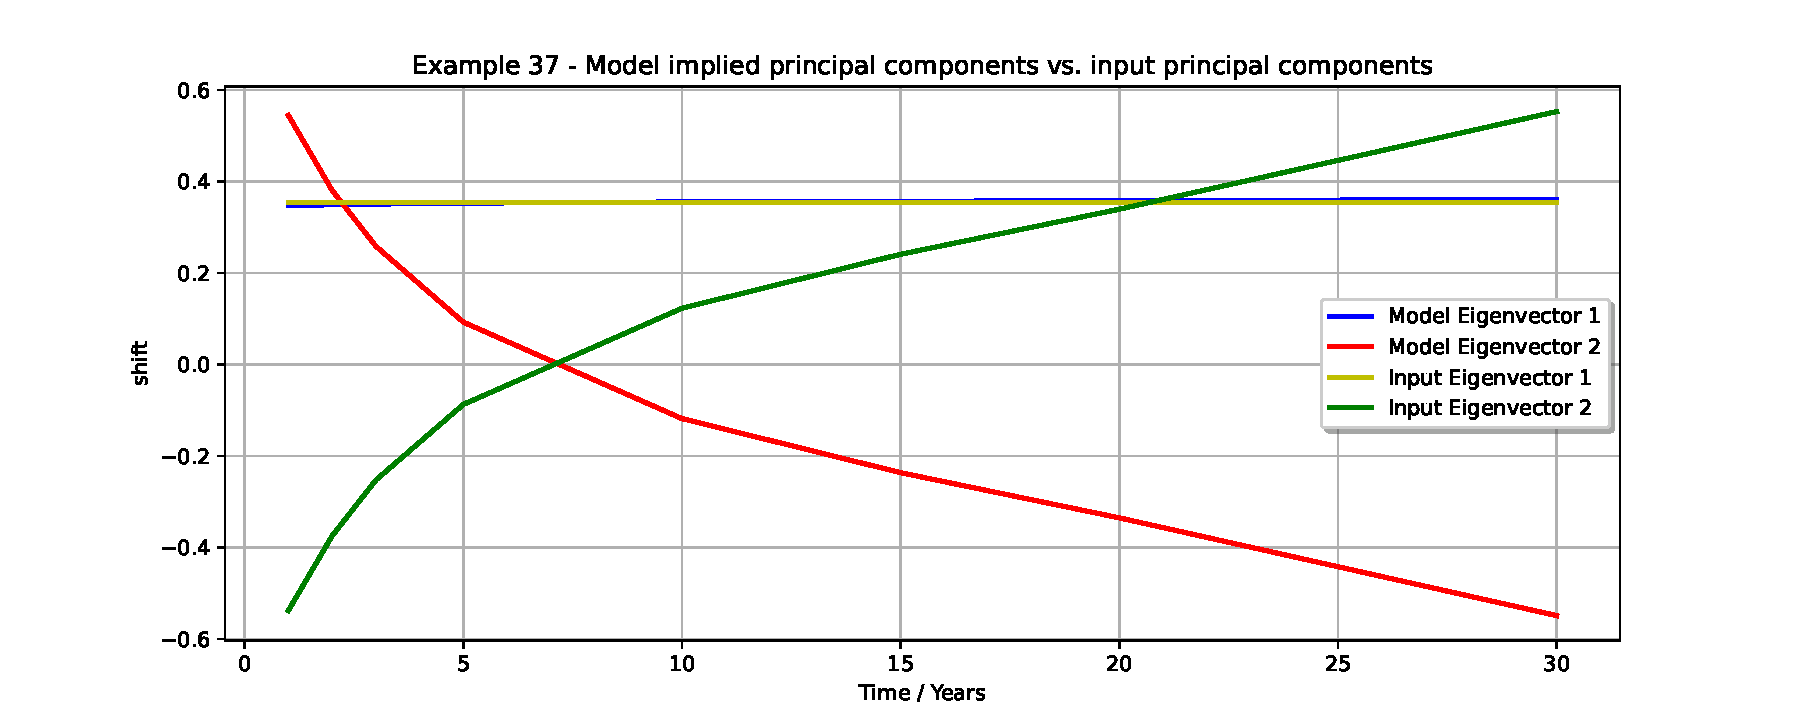
\includegraphics[scale=0.50]{mpl_eigenvectors_ex37.pdf}
\end{center}
\caption{Input and model implied eigenvectors for a Hull-White 4-factor model calibrated to 2 principal components of
  rate curve movements (parallel + rotation). Notice that the model implied 2nd eigenvector is the negative of the input
  vector.}
\label{fig:ex37}
\end{figure}

%--------------------------------------------------------------------
\subsection{Cross Currency Swap Exposure using Multifactor Hull-White Models}% Example 38
\label{example:38}
%--------------------------------------------------------------------

The example in folder {\tt Examples/Example\_38} is similar to Example 8 (EPE, ENE for xccy swap), but uses a
multifactor HW model for EUR and USD to generate scenarios. The parametrization of the HW models is taken from Example
37.

Each of the two factors of each HW model is correlated with each of the two factors of the other currency's HW model and
with the FX factors. Remember that the factors represent principal components of interest rate movements and so the
correlations can be interpreted as correlations of these principal components with each other and the fx rate processes.

%--------------------------------------------------------------------
\subsection{Exposure Simulation using American Monte Carlo}% Example 39
\label{example:39}
%--------------------------------------------------------------------

The example in folder {\tt Examples/Example\_39} demonstrates how to use American Monte Carlo simulation (AMC) to generate exposures in ORE.
For a sketch of the methodology and comments on its implementation in ORE see appendix \ref{sec:app_amc}.

Calling 

\medskip
\centerline {\tt python run.py} 

\medskip
performs two ORE runs, a 'classical' exposure simulation and an American Monte Carlo simulation, both on a quarterly simulation grid and for the same portfolio consisting of four trades:

\begin{itemize}
\item Bermudan swaption
\item Single Currency Swap
\item Cross Currency Swap
\item FX Option
\end{itemize}

We use a 'flat' market here (yield curve and Swaption volatility surface). The number of simulation paths is 2k in the classic simulations. If not stated otherwise below, the number of training paths and simulation paths is 10k in the AMC simulations. 

In the following we compare the AMC exposure profiles to those produced by the 'classic' valuation engine for each trade and the netting set. 

Figure \ref{epe_swaption} shows the EPE and ENE for a Bermudan Swaption 10y into 10y in (base ccy) EUR with physical settlement. The classic run uses
the LGM grid engine for valuation. We observe close agreement between the two runs. To achieve the observed agreement, it is essential to set the LGM model's mean reversion speed to zero in both
\begin{itemize}
\item the Bermudan Swaption LGM pricing model (see Input/pricingengine.xml), and
\item the Cross Asset Model's IR model components (see Input/simulation.xml and Input/simulation\_amc.xml) 
\end{itemize}
and to use a high order 6 of the regression polynomials (see Input/pricingengine\_amc.xml).
 
\begin{figure}
  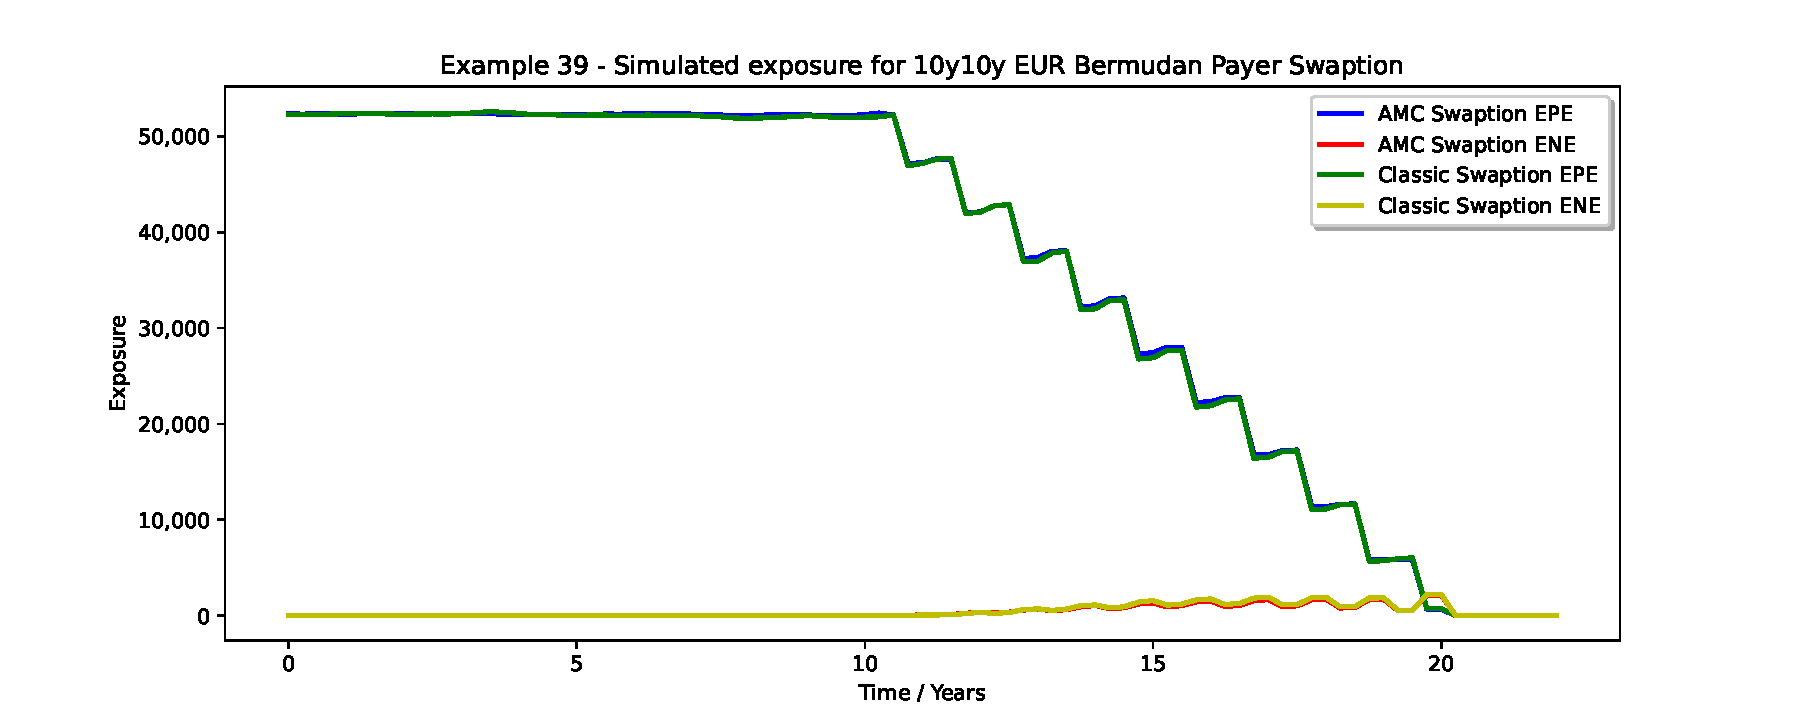
\includegraphics[width=0.8\textwidth]{mpl_amc_bermudanswaption.pdf}
  \caption{EPE of a EUR Bermudan Swaption computed with the classic and AMC valuation engines, using 50k training paths for the AMC simulation.}
  \label{epe_swaption}
\end{figure}

Figure \ref{epe_swap} shows the EPE and ENE for a 20y vanilla Swap in USD. The currency of
the amc calculator is USD in this case, i.e. it is different from the base ccy of the simulation (EUR). The consistency
of the classic and amc runs in particular demonstrates the correct application of the currency conversion factor
\ref{currency_conversion_factor}. To get a better accuracy for purposes of the plot in this document we increased the
number of training paths for this example to 50k and the order of the basis functions to 6.

\begin{figure}
  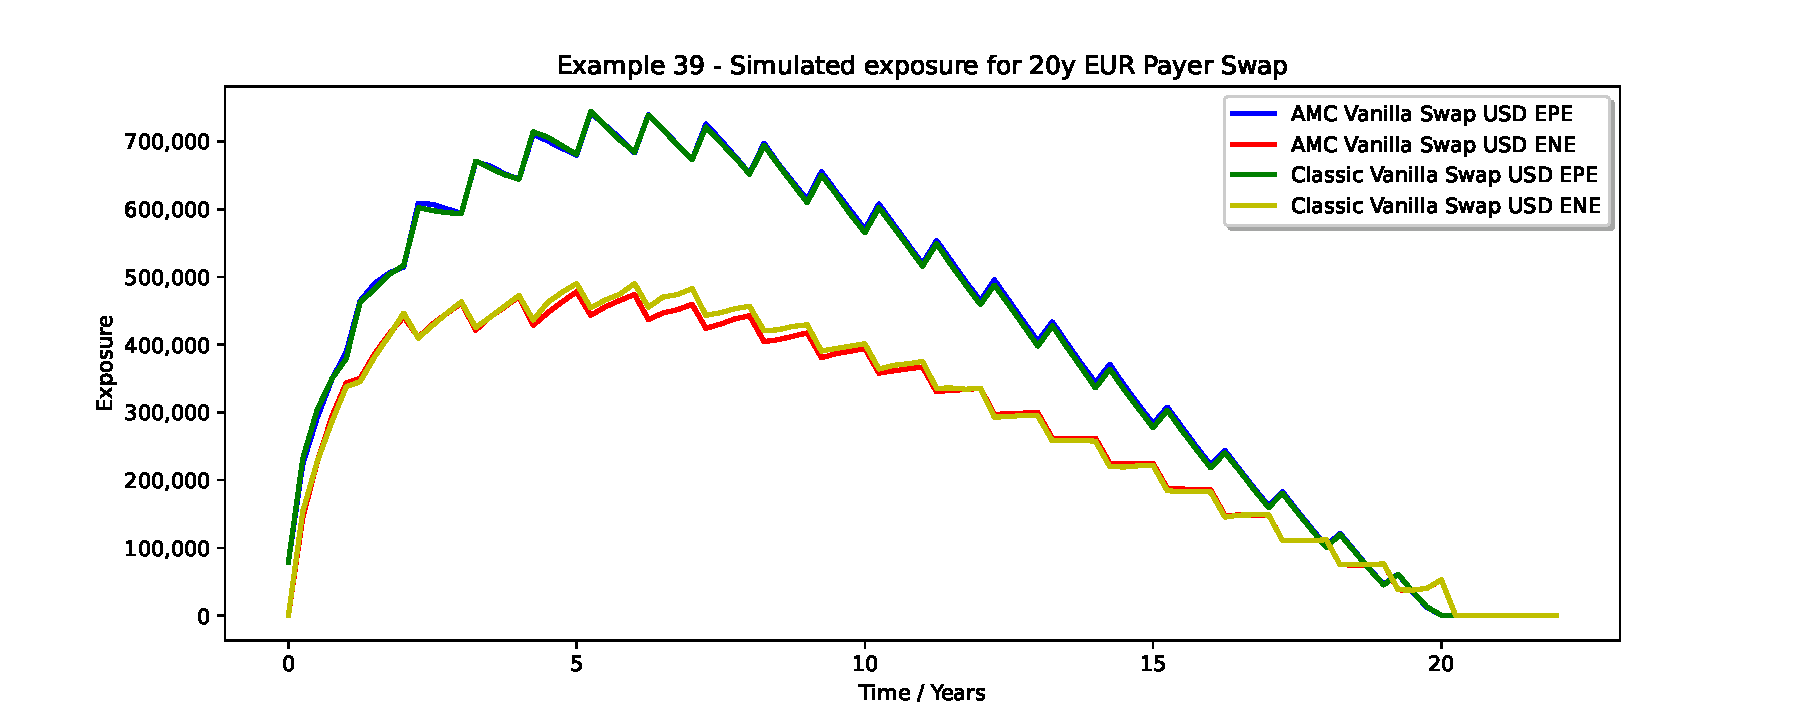
\includegraphics[width=0.8\textwidth]{mpl_amc_vanillaswap_usd.pdf}
  \caption{EPE of a USD swap computed with the classic and AMC valuation engines}
  \label{epe_swap}
\end{figure}

Figure \ref{epe_ccyswap} shows the EPE and ENE for a 20y cross currency Swap EUR-USD. 

\begin{figure}
  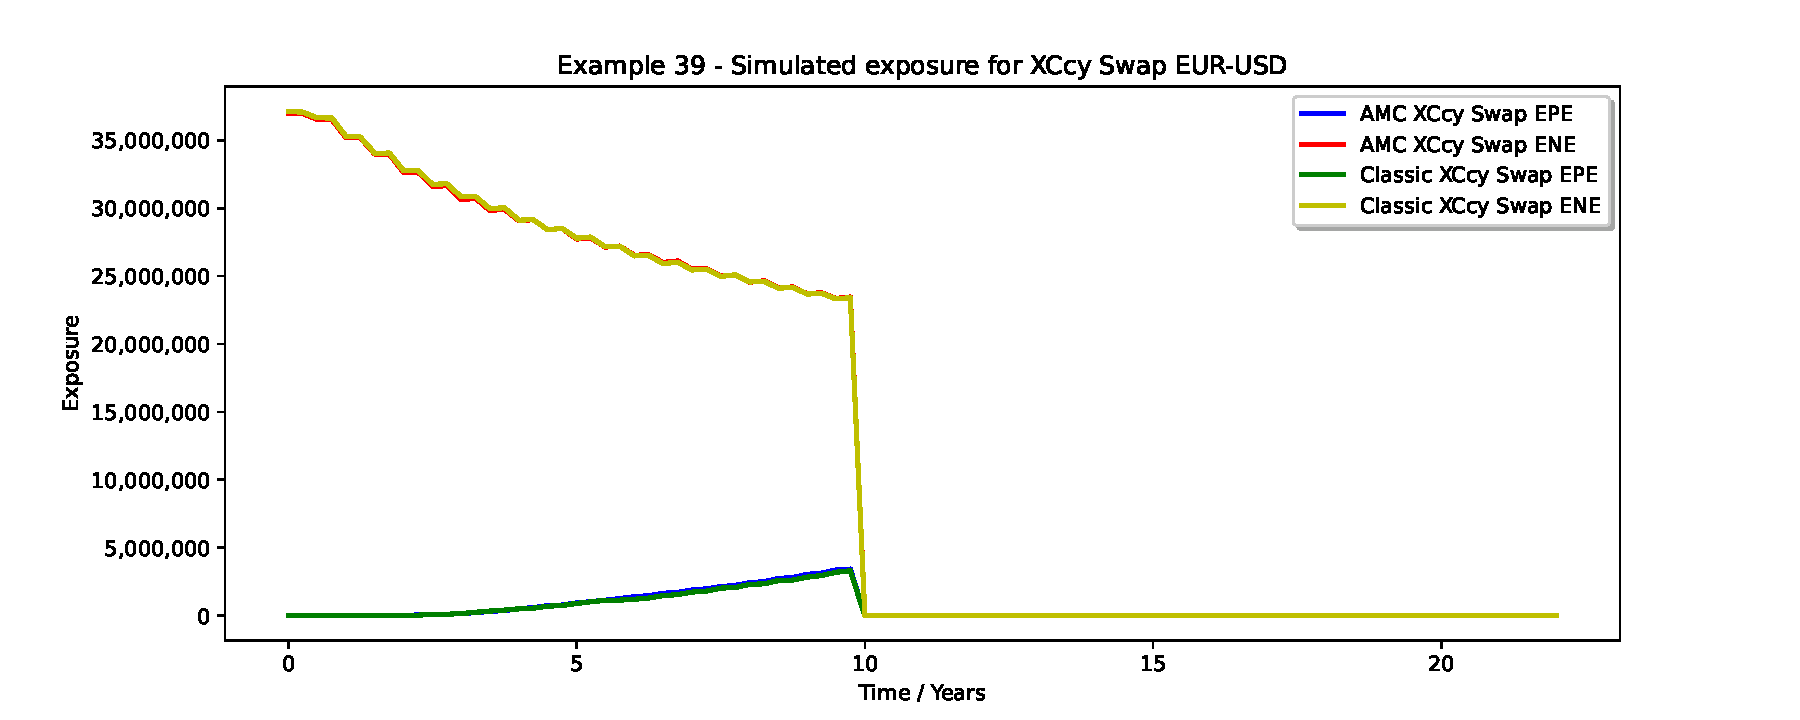
\includegraphics[width=0.8\textwidth]{mpl_amc_xccyswap.pdf}
  \caption{EPE of a EUR-USD cross currency swap computed with the classic and AMC valuation engines}
  \label{epe_ccyswap}
\end{figure}

Figure \ref{epe_fxoption} shows the EPE and ENE for a vanilla FX Option EUR-USD with 10y1m expiry. 
For the classic run the FX volatility surface is not implied by the cross asset model but kept flat, which
yields a slight hump in the profile. The AMC profile is flat on the other hand which demonstrates the consistency of the
FX Option pricing with the risk factor evolution model.

\begin{figure}
  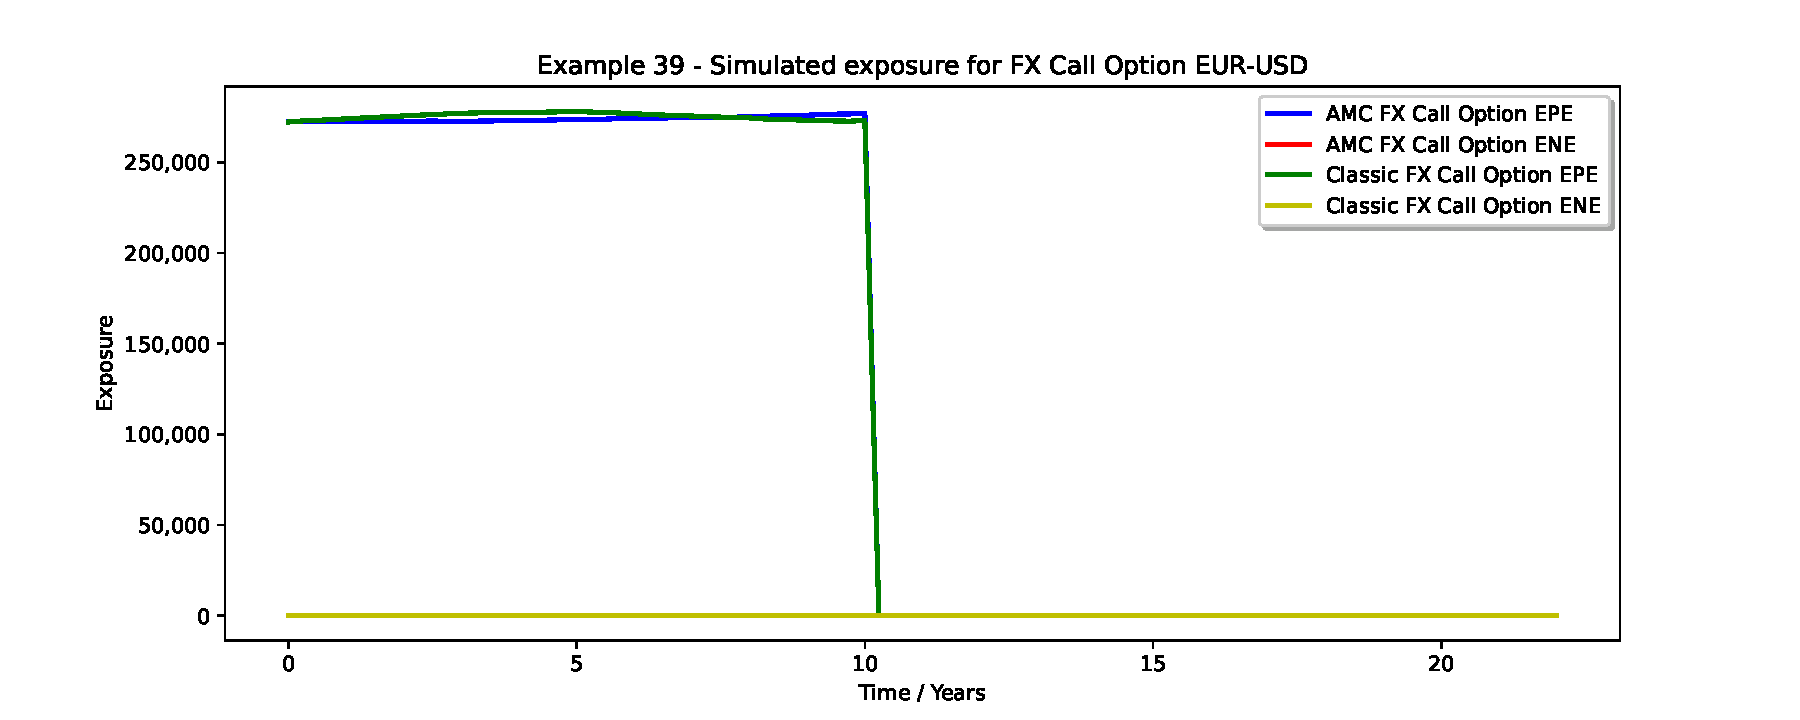
\includegraphics[width=0.8\textwidth]{mpl_amc_fxoption.pdf}
  \caption{EPE of a EUR-USD FX option computed with the classic and AMC valuation engines}
  \label{epe_fxoption}
\end{figure}

\subsubsection*{Analytic Configuration}
\label{sec:amc_applicationconfig}

To use the AMC engine for an XVA simulation the following needs to be added to the {\tt simulation} analytic in {\tt ore.xml}:

\begin{minted}[fontsize=\scriptsize]{xml}
<Analytic type="simulation">
  ...
  <Parameter name="amc">Y</Parameter>
  <Parameter name="amcPricingEnginesFile">pricingengine_amc.xml</Parameter>
  <Parameter name="amcTradeTypes">Swaption</Parameter>
  ...
</Analytic>
\end{minted}

The trades which have a trade type matching one of the types in the \verb+amcTradeTypes+ list, will be built against the
pricing engine config provided and processed in the AMC engine. As a naming convention, pricing engines with engine type
AMC provide the required functionality to be processed by the AMC engine, for technical details cf. \ref{sec:app_amc}.

All other trades are processed by the classic simulation engine in ORE. The resulting cubes from the classic and AMC
simulation are joined and passed to the post processor in the usual way.

Note that since sometimes the AMC pricing engines have a different base ccy than the risk factor evolution model (see
below), a horizon shift parameter in the simulation set up should be set for all currencies, so that the shift also
applies to these reduced models.

\subsubsection*{Pricing Engine Configuration}
\label{sec:amc_pricingengineconfig}

At this point we assume that the reader is generally familiar with the configuration section 
\ref{sec:configuration}, in particular pricing engine configuration in section \ref{sec:configuration_pricingengines}.

The pricing engine configuration is similar for all AMC enabled products, e.g. for Bermudan Swaptions:

\begin{minted}[fontsize=\scriptsize]{xml}
<Product type="BermudanSwaption">
  <Model>LGM</Model>
  <ModelParameters/>
  <Engine>AMC</Engine>
  <EngineParameters>
    <Parameter name="Training.Sequence">MersenneTwisterAntithetic</Parameter>
    <Parameter name="Training.Seed">42</Parameter>
    <Parameter name="Training.Samples">50000</Parameter>
    <Parameter name="Training.BasisFunction">Monomial</Parameter>
    <Parameter name="Training.BasisFunctionOrder">6</Parameter>
    <Parameter name="Pricing.Sequence">SobolBrownianBridge</Parameter>
    <Parameter name="Pricing.Seed">17</Parameter>
    <Parameter name="Pricing.Samples">0</Parameter>
    <Parameter name="BrownianBridgeOrdering">Steps</Parameter>
    <Parameter name="SobolDirectionIntegers">JoeKuoD7</Parameter>
    <Parameter name="MinObsDate">true</Parameter>
    <Parameter name="RegressionOnExerciseOnly">false</Parameter>
  </EngineParameters>
</Product>
\end{minted}

The \verb+Model+ differs by product type, table \ref{tbl:amcconfig} summarises the supported product types and model and
engine types. The engine parameters are the same for all products:

\begin{enumerate}
\item \verb+Training.Sequence+: The sequence type for the traning phase, can be \verb+MersenneTwister+,
  \verb+MersenneTwisterAntithetc+, \verb+Sobol+, \verb+Burley2020Sobol+, \verb+SobolBrownianBridge+,
  \verb+Burley2020SobolBrownianBridge+
\item \verb+Training.Seed+: The seed for the random number generation in the training phase
\item \verb+Training.Samples+: The number of samples to be used for the training phase
\item \verb+Pricing.Sequence+: The sequence type for the pricing phase, same values allowed as for training
\item \verb+Training.BasisFunction+: The type of basis function system to be used for the regression analysis, can be
  \verb+Monomial+, \verb+Laguerre+, \verb+Hermite+, \verb+Hyperbolic+, \verb+Legendre+, \verb+Chbyshev+,
  \verb+Chebyshev2nd+
\item \verb+BasisFunctionOrder+: The order of the basis function system to be used
\item \verb+Pricing.Seed+: The seed for the random number generation in the pricing
\item \verb+Pricing.Samples+: The number of samples to be used for the pricing phase. If this number is zero, no pricing
  run is performed, instead the (T0) NPV is estimated from the training phase (this result is used to fill the T0 slice
  of the NPV cube)
\item \verb+BrownianBridgeOrdering+: variate ordering for Brownian bridges, can be \verb+Steps+, \verb+Factors+,
  \verb+Diagonal+
\item \verb+SobolDirectionIntegers+: direction integers for Sobol generator, can be \verb+Unit+, \verb+Jaeckel+,
  \verb+SobolLevitan+, \verb+SobolLevitanLemieux+, \verb+JoeKuoD5+, \verb+JoeKuoD6+, \verb+JoeKuoD7+,
  \verb+Kuo+, \verb+Kuo2+, \verb+Kuo3+
\item \verb+MinObsDate+: if true the conditional expectation of each cashflow is taken from the minimum possible
  observation date (i.e. the latest exercise or simulation date before the cashflow's event date); recommended setting
  is \verb+true+
\item \verb+RegressionOnExerciseOnly+: if true, regression coefficients are computed only on exercise dates and
  extrapolated (flat) to earlier exercise dates; only for backwards compatibility to older versions of the AMC module,
  recommended setting is \verb+false+
\end{enumerate}

\begin{table}[hbt]
  \begin{tabular}{l|l|l}
    Product Type & Model & Engine \\ \hline
    Swap & CrossAssetModel & AMC \\
    CrossCurrencySwap & CrossAssetModel & AMC \\
    FxOption & CrossAssetModel & AMC \\
    BermudanSwaption & LGM & AMC \\
    MultiLegOption & CrossAssetModel & AMC \\
  \end{tabular}
  \caption{AMC enabled products with engine and model types}
  \label{tbl:amcconfig}
\end{table}

\subsubsection*{Additional Features}
\label{sec:amc_sideproducts}

As a side product the AMC module provides plain MC pricing engines for Bermudan Swaptions and a new trade type
\verb+MultiLegOption+ with a corresponding MC pricing engine.

\subsubsection*{MC pricing engine for Bermudan swaptions}\label{sec:mc_bermudan_engine}

The following listing shows a sample configuration for the MC Bermudan Swaption engine. The model parameters are
identical to the LGM Grid engine configuration. The engine parameters on the other hand are the same as for the AMC
engine, see \ref{sec:amc_pricingengineconfig}.

\begin{minted}[fontsize=\scriptsize]{xml}
<Product type="BermudanSwaption">
  <Model>LGM</Model>
  <ModelParameters>
    <Parameter name="Calibration">Bootstrap</Parameter>
    <Parameter name="CalibrationStrategy">CoterminalDealStrike</Parameter>
    <Parameter name="Reversion_EUR">0.0050</Parameter>
    <Parameter name="Reversion_USD">0.0030</Parameter>
    <Parameter name="ReversionType">HullWhite</Parameter>
    <Parameter name="VolatilityType">HullWhite</Parameter>
    <Parameter name="Volatility">0.01</Parameter>
    <Parameter name="ShiftHorizon">0.5</Parameter>
    <Parameter name="Tolerance">1.0</Parameter>
  </ModelParameters>
  <Engine>MC</Engine>
  <EngineParameters>
    <Parameter name="Training.Sequence">MersenneTwisterAntithetic</Parameter>
    <Parameter name="Training.Seed">42</Parameter>
    <Parameter name="Training.Samples">10000</Parameter>
    <Parameter name="Training.BasisFunction">Monomial</Parameter>
    <Parameter name="Training.BasisFunctionOrder">6</Parameter>
    <Parameter name="Pricing.Sequence">SobolBrownianBridge</Parameter>
    <Parameter name="Pricing.Seed">17</Parameter>
    <Parameter name="Pricing.Samples">25000</Parameter>
    <Parameter name="BrownianBridgeOrdering">Steps</Parameter>
    <Parameter name="SobolDirectionIntegers">JoeKuoD7</Parameter>
  </EngineParameters>
</Product>
\end{minted}

\subsubsection*{Multi Leg Options / MC pricing engine}

The following listing shows a sample MultiLegOption trade. It consists of

\begin{enumerate}
\item an option data block; this is optional, see below
\item a number of legs; in principle all leg types are supported, the number of legs is arbitrary and they can be in
  different currencies; if the payment currency of a leg is different from a floating index currency, this is
  interpreted as a quanto payoff
\end{enumerate}

If the option block is given, the trade represents a Bermudan swaption on the underlying legs. If the option block is
missing, the legs themselves represent the trade.

See \ref{sec:amc_limitations} for limitations of the multileg option pricing engine.

\begin{minted}[fontsize=\scriptsize]{xml}
<Trade id="Sample_MultiLegOption">
  <TradeType>MultiLegOption</TradeType>
  <Envelope>...</Envelope>
  <MultiLegOptionData>
    <OptionData>
      <LongShort>Long</LongShort>
      <OptionType>Call</OptionType>
      <Style>Bermudan</Style>
      <Settlement>Physical</Settlement>
      <PayOffAtExpiry>false</PayOffAtExpiry>
      <ExerciseDates>
        <ExerciseDate>2026-02-25</ExerciseDate>
        <ExerciseDate>2027-02-25</ExerciseDate>
        <ExerciseDate>2028-02-25</ExerciseDate>
      </ExerciseDates>
    </OptionData>
    <LegData>
      <LegType>Floating</LegType>
      <Payer>false</Payer>
      <Currency>USD</Currency>
      <Notionals>
        <Notional>100000000</Notional>
      </Notionals>
      ...
    </LegData>
    <LegData>
      <LegType>Floating</LegType>
      <Payer>true</Payer>
      <Currency>EUR</Currency>
      <Notionals>
        <Notional>100000000</Notional>
      </Notionals>
      ...
    </LegData>
  </MultiLegOptionData>
</Trade>
\end{minted}

The pricing engine configuration is similar to that of the MC Bermudan swaption engine, cf.
\ref{sec:mc_bermudan_engine}, also see the following listing.

\begin{minted}[fontsize=\scriptsize]{xml}
  <Product type="MultiLegOption">
  <Model>CrossAssetModel</Model>
  <ModelParameters>
    <Parameter name="Tolerance">0.0001</Parameter>
    <!-- IR -->
    <Parameter name="IrCalibration">Bootstrap</Parameter>
    <Parameter name="IrCalibrationStrategy">CoterminalATM</Parameter>
    <Parameter name="ShiftHorizon">1.0</Parameter>
    <Parameter name="IrReversion_EUR">0.0050</Parameter>
    <Parameter name="IrReversion_GBP">0.0070</Parameter>
    <Parameter name="IrReversion_USD">0.0080</Parameter>
    <Parameter name="IrReversion">0.0030</Parameter>
    <Parameter name="IrReversionType">HullWhite</Parameter>
    <Parameter name="IrVolatilityType">HullWhite</Parameter>
    <Parameter name="IrVolatility">0.0050</Parameter>
    <!-- FX -->
    <Parameter name="FxCalibration">Bootstrap</Parameter>
    <Parameter name="FxVolatility_EURUSD">0.10</Parameter>
    <Parameter name="FxVolatility">0.08</Parameter>
    <Parameter name="ExtrapolateFxVolatility_EURUSD">false</Parameter>
    <Parameter name="ExtrapolateFxVolatility">true</Parameter>
    <!-- Correlations IR-IR, IR-FX, FX-FX -->
    <Parameter name="Corr_IR:EUR_IR:GBP">0.80</Parameter>
    <Parameter name="Corr_IR:EUR_FX:GBPEUR">-0.50</Parameter>
    <Parameter name="Corr_IR:GBP_FX:GBPEUR">-0.15</Parameter>
  </ModelParameters>
  <Engine>MC</Engine>
  <EngineParameters>
    <Parameter name="Training.Sequence">MersenneTwisterAntithetic</Parameter>
    <Parameter name="Training.Seed">42</Parameter>
    <Parameter name="Training.Samples">10000</Parameter>
    <Parameter name="Pricing.Sequence">SobolBrownianBridge</Parameter>
    <Parameter name="Pricing.Seed">17</Parameter>
    <Parameter name="Pricing.Samples">25000</Parameter>
    <Parameter name="Training.BasisFunction">Monomial</Parameter>
    <Parameter name="Training.BasisFunctionOrder">4</Parameter>
    <Parameter name="BrownianBridgeOrdering">Steps</Parameter>
    <Parameter name="SobolDirectionIntegers">JoeKuoD7</Parameter>
  </EngineParameters>
</Product>
\end{minted}

Model Parameters special to that product are

\begin{enumerate}
\item \verb+IrCalibrationStrategy+ can be \verb+None+, \verb+CoterminalATM+, \verb+UnderlyingATM+
\item \verb+FXCalibration+ can be \verb+None+ or \verb+Bootstrap+
\item \verb+ExtrapolateFxVolatility+ can be \verb+true+ or \verb+false+; if false, no calibration instruments are used
  that require extrapolation of the market fx volatilty surface in option expiry direction
\item \verb+Corr_Key1_Key2+: These entries describe the cross asset model correlations to be used; the syntax for
  \verb+Key1+ and \verb+Key2+ is the same as in the simulation configuration for the cross asset model
\end{enumerate}

%--------------------------------------------------------------------
\subsection{Par Sensitivity Analysis}% Example 40
\label{example:40}
%--------------------------------------------------------------------

The example in folder {\tt Examples/Example\_40}  demonstrates ORE's par sensitivity analysis (e.g. to Swap rates) 
that is implemented  by means of a Jacobi transformation of the "raw" sensitivities (e.g. to zero rates), see a sketch of the 
methodology in appendix \ref{app:par_sensi} and section \ref{sec:sensitivity} for configuration details.

To perform a par sensitivity analysis, the following required change in {\tt ore.xml} is required

\begin{minted}[fontsize=\scriptsize]{xml}
    <Analytic type="sensitivity">
      <Parameter name="active">Y</Parameter>
      <Parameter name="marketConfigFile">simulation.xml</Parameter>
      <Parameter name="sensitivityConfigFile">sensitivity.xml</Parameter>
      <Parameter name="pricingEnginesFile">../../Input/pricingengine.xml</Parameter>
      <Parameter name="scenarioOutputFile">sensi_scenarios.csv</Parameter>
      <Parameter name="sensitivityOutputFile">sensitivity.csv</Parameter>
      <Parameter name="outputSensitivityThreshold">0.000001</Parameter>
      <!-- Additional parametrisation for par sensitivity analysis -->
      <Parameter name="parSensitivity">Y</Parameter>
      <Parameter name="parSensitivityOutputFile">parsensitivity.csv</Parameter>
      <Parameter name="outputJacobi">Y</Parameter>
      <Parameter name="jacobiOutputFile">jacobi.csv</Parameter>
      <Parameter name="jacobiInverseOutputFile">jacobi_inverse.csv</Parameter>
    </Analytic>
\end{minted}

The portfolio used in this example includes products sensitive to 
\begin{itemize}
\item Discount and index curves
\item Credit curves
\item Inflation curves
\item CapFloor volatilities
\end{itemize}

The usual sensitivity analysis is performed by bumping the "raw" rates (zero rates, hazard rates, inflation zero rates, optionlet vols).
This is followed by the Jacobi transformation that turns "raw" sensitivities  into sensitivities in the par domain (Deposit/FRA/Swap rates, FX Forwards, CC Basis Swap spreads, 
CDS spreads, ZC and YOY Inflation Swap rates, flat Cap/Floor vols). The conversion is controlled by the additional {\tt ParConversion} data blocks 
in {\tt sensitivity.xml} where the assumed par instruments and corresponding conventions are coded, as shown below for three types of discount curves.

\begin{minted}[fontsize=\scriptsize]{xml}
  <DiscountCurves>
  
    <DiscountCurve ccy="EUR">
      <ShiftType>Absolute</ShiftType>
      <ShiftSize>0.0001</ShiftSize>
      <ShiftTenors>2W,1M,3M,6M,9M,1Y,2Y,3Y,4Y,5Y,7Y,10Y,15Y,20Y,25Y,30Y</ShiftTenors>
      <ParConversion>
        <!--DEP, FRA, IRS, OIS, FXF, XBS -->
	<Instruments>OIS,OIS,OIS,OIS,OIS,OIS,OIS,OIS,OIS,OIS,OIS,OIS,OIS,OIS,OIS,OIS</Instruments>
	<SingleCurve>true</SingleCurve>
	<Conventions>
	  <Convention id="OIS">EUR-OIS-CONVENTIONS</Convention>
	</Conventions>
      </ParConversion>
    </DiscountCurve>   
    
    <DiscountCurve ccy="USD">
      <ShiftType>Absolute</ShiftType>
      <ShiftSize>0.0001</ShiftSize>
      <ShiftTenors>2W,1M,3M,6M,9M,1Y,2Y,3Y,4Y,5Y,7Y,10Y,15Y,20Y,25Y,30Y</ShiftTenors>
      <ParConversion>
	<Instruments>FXF,FXF,FXF,FXF,FXF,XBS,XBS,XBS,XBS,XBS,XBS,XBS,XBS,XBS,XBS,XBS</Instruments>
	<SingleCurve>true</SingleCurve>
	<Conventions>
	  <Convention id="XBS">EUR-USD-XCCY-BASIS-CONVENTIONS</Convention>
	  <Convention id="FXF">EUR-USD-FX-CONVENTIONS</Convention>
	</Conventions>
      </ParConversion>

    <DiscountCurve ccy="GBP">
      <ShiftType>Absolute</ShiftType>
      <ShiftSize>0.0001</ShiftSize>
      <ShiftTenors>2W,1M,3M,6M,9M,1Y,2Y,3Y,4Y,5Y,7Y,10Y,15Y,20Y,25Y,30Y</ShiftTenors>
      <ParConversion>
	<Instruments>DEP,DEP,DEP,DEP,DEP,IRS,IRS,IRS,IRS,IRS,IRS,IRS,IRS,IRS,IRS,IRS</Instruments>
	<SingleCurve>true</SingleCurve>
	<Conventions>
	  <Convention id="DEP">GBP-DEPOSIT</Convention>
	  <Convention id="IRS">GBP-6M-SWAP-CONVENTIONS</Convention>
	</Conventions>
      </ParConversion>
    </DiscountCurve>
  
  </DiscountCurves>
\end{minted}

Finally note that par sensitivity analysis requires that the shift tenor grid in the sensitivity data above matches the corresponding grid in the simulation (market) configuration.
See also section \ref{sec:sensitivity}.

%--------------------------------------------------------------------
\subsection{Multi-threaded Exposure Simultion}% Example 41
\label{example:41}
%--------------------------------------------------------------------

The example in folder {\tt Examples/Example\_41} demonstrates the multithreaded valuation engine to generate the exposure for a
portfolio of 8 copies of the vanilla swap in {\tt Example\_1}.

%--------------------------------------------------------------------
\subsection{ORE Python Module}% Example 42
\label{example:42}
%--------------------------------------------------------------------

Since release 9 (March 2023) we provide easy access to ORE via a pre-compiled Python module. Some example scripts using this ORE module are provided in this example, so change to this directory first

\medskip
{\tt cd Example\_42} 

\medskip
The examples require Python 3. The ORE Python module is then installed with a one-liner, see step 3 below. However, to separate ORE from any other Python environments on your machine, we recommend creating a virtual environment first. In that case the steps are as follows. 

\begin{enumerate}
\item To create a virtual environment: {\tt python -m venv env1} 
\item To activate this environment on Windows: {\tt .{\bs}env1{\bs}Scripts{\bs}activate.bat}  \\
or on macOS/Linux: {\tt ./env1/bin/activate }  
\item Then install the latest release of ORE:\\
{\tt pip install open-source-risk-engine } 
\item Try examples:\\
	\begin{itemize} 
	\item {\tt python ore.py} \\
	This demonstrates the Python-wrapped version of the ORE application that is also used in the command line application {\tt ore.exe}. We use it here to re-run the Swap exposure of {\tt Example\_1}. 
	\item {\tt python ore2.py} \\
	This extends the previous example and shows how to access and post-process ORE in-memory results in the Python framework without reading files. 
	\item {\tt python commodityforward.py} \\
	The ORE Python module also allows lower-level access to the QuantLib and QuantExt libraries, demonstrated here for a CommodityForward instrument defined in QuantExt. 
	Note that the ORE Python module contains the entire QuantLib Python functionality.
	\end{itemize}
	More use cases of the ORE Python module including Jupyter notebooks can be found in the ORE SWIG repository, in particular in folder OREAnalytics-SWIG/Python/Examples. 
\item You can deactivate the environment with {\tt deactivate} \\
or even fully remove the environment again by removing the {\tt env1} folder.
\end{enumerate}

Finally, you can build the Python module and installable packages yourself following the instructions in sections \ref{sec:oreswig}, \ref{sec:win_wheel}, \ref{sec:nix_wheel}
based on your local ORE code. 

%--------------------------------------------------------------------
\subsection{Credit Portfolio Model}% Example 43
\label{example:43}
%--------------------------------------------------------------------

The purpose of the credit portfolio model in ORE is to generate an integrated portfolio gain/loss distribution at a given future horizon which is driven by 
\begin{itemize}
\item credit defaults and rating migrations in Bonds and CDS, and 
\item the PnL of a portfolio of derivatives over the specified time horizon.
\end{itemize}
The model integrates Credit and Market Risk by jointly evolving systemic credit risk drivers alongside the usual risk factors in ORE's Cross Asset Model.
See also the separate documentation in Docs/UserGuide/creditmodel.tex.

By running \\
\medskip
\centerline{{\tt python run.py}} 

\medskip
this example demonstrates the model's outcome for seven demo portfolios

\begin{center}
\begin{tabular}{|l|l|l|l|}
\hline
Case & Credit Mode & Exposure Mode & Evaluation \\
\hline
\hline
Single Bond & Migration & Value & Analytic \\
\hline
Bond and Swap & Migration & Value & Analytic \\
\hline
3 Bonds & Migration & Value & Analytic \\
\hline
10 Bonds & Migration & Value & Analytic \\
\hline
10 Bonds & Migration & Value & Terminal Simulation \\
\hline
Bonds and CDS & Migration & Notional & Analytic \\
\hline
100 Bonds & Default & Notional & Analytic \\
\hline
\end{tabular}
\end{center}
The last demo case in this table can be activated by uncommenting the corresponding section at the end of the {\tt run.py} script.
 
%--------------------------------------------------------------------
\subsection{ISDA SIMM Model}% Example 44
\label{example:44}
%--------------------------------------------------------------------

This example demonstrates the calculation of initial margin using ISDA's Standard Initial Margin Model (SIMM) based on a provided 
sensitivity file in ISDA's Common Risk Interchange Format (CRIF).
ORE covers all SIMM versions since inception to date, i.e.\ 1.0, 1.1, 1.2, 1.3, 1.3.38, 2.0, 2.1, 2.2, 2.3, 2.4 (=2.3.8), 2.5, 2.5A, 2.6 (=2.5.6).
All versions have been tested against the respective ISDA SIMM model unit test suites and pass these tests.
Any new SIMM versions will be added with each ORE release.

For SIMM versions >= 2.2 we support SIMM calculation for both MPoR horizons, 1d and 10d.
 
Note that you need to purchase a SIMM model license from ISDA if you want to use the model in production, and the unit test
suites mentioned above are provided to licensed vendors only. Therefore we unfortunately cannot share our ORE SIMM model 
test suite here either. 

By running \\
\medskip
\centerline{{\tt python run.py}} 

\medskip
ORE will pick up the small example CRIF file in {\tt Input/crif.csv} (i.e.\ par sensitivities rebucketed and reformatted to match the ISDA CRIF template) and generate the resulting SIMM report in a {\tt simm.csv} file.
This report shows ISDA SIMM results with the usual breakdown by product class, risk class, margin type, bucket and SIMM ``side'' (IM to call or post).
The SIMM calculation in this example is done for SIMM version 2.4 and 2.6, with MPoR 1d and 10d:

\begin{itemize}
  \item SIMM 2.4, 1-day MPoR
  \item SIMM 2.4, 10-day MPoR
  \item SIMM 2.6, 1-day MPoR
  \item SIMM 2.6, 10-day MPoR
\end{itemize}

\medskip
There are four input files -- {\tt ore\_SIMM2.4\_1D.xml}, {\tt ore\_SIMM2.4\_10D.xml}, {\tt ore\_SIMM2.6\_1D.xml}, {\tt ore\_SIMM2.6\_10D.xml} -- with corresponding folders in the {\tt Output/} directory.
The relevant inputs in the files are:

\begin{itemize}
\item SIMM version
\item name of the CRIF file to be loaded
\item calculation currency - this determines which Risk\_FX entries of the CRIF will be ignored in the SIMM calculation
\item result currency (optional) - currency of the resulting SIMM amounts in the report, by default equal to the calculation currency
\item MPoR horizon, in terms of days
\end{itemize}

The market data input and todays's market configuration required here is minimal - limited to FX rates for conversions from base/calculation currency into USD and into the result currency.

\bigskip
If the ORE Python module is installed, as shown in Example 42, then you can also run the SIMM example using

\medskip
\centerline{\tt python ore.py} 

%--------------------------------------------------------
\subsection{Collateralized Bond Obligation}% Example 45
%--------------------------------------------------------

This example in folder {\tt Examples/Example\_45} demonstrates a Cashflow CDO or Collateralized Bond Obligation (CBO) via ORE. Calling

\medskip
\centerline{\tt python run.py}

\medskip
will launch a single ORE run to process a CBO example, referencing underyling bond portfolio of 20 trades. 
The CBO is represented by a CBO reference datum specified in the reference data file. 
NPV results are calculated for the investment in the junior tranche. 

%--------------------------------------------------------
\subsection{Generic Total Return Swap}% Example 46
%--------------------------------------------------------

This example in folder {\tt Examples/Example\_46} demonstrates ORE's generic Total Return Swap referencing a CBO. 
Calling

\medskip
\centerline{\tt python run.py}

\medskip
will launch a single ORE run to process a TRS example and to generate NPV and cash flows in the usual result files.
As opposed to example 45, the CBO and its bondbasket are represented explicitly in the CBO node.

%--------------------------------------------------------
\subsection{Composite Trade}% Example 47
%--------------------------------------------------------

This example in folder {\tt Examples/Example\_47} demonstrates the input of ORE's Composite Trade that can consist on any number 
and type of products covered by ORE. In this case the composite consists of two Equity Swaps.
Calling

\medskip
\centerline{\tt python run.py}

\medskip
runs ORE and generates an NPV report.

%--------------------------------------------------------
\subsection{Convertible Bond and ASCOT}% Example 48
%--------------------------------------------------------

This example in folder {\tt Examples/Example\_48} demonstrates the input of 
\begin{itemize}
\item a ConvertibleBond  trade
\item a related Asset Swapped Convertible Option Transaction (ASCOT)
\item a vanilla Swap that represents the package of Convertible Bond position and ASCOT
\end{itemize}

Calling
\medskip
\centerline{\tt python run.py}

\medskip
runs ORE and generates an NPV report.

%--------------------------------------------------------
\subsection{Bond Yield Shifted}% Example 49
\label{example:49}
%--------------------------------------------------------

The example in folder {\tt Examples/Example\_49} shows how to use a yield curve
built from a BondYieldShifted segment, as described in section \ref{sec:bond_yield_shifted}.

In particular, it builds the curve {\tt USD.BMK.GVN.CURVE\_SHIFTED} shifted by three liquid Bonds:

\begin{itemize}
\item Fixed rate USD Bond maturing in August 2023 with id {\tt EJ7706660}.
\item Fixed rate USD Bond maturing in September 2049 with id {\tt ZR5330686}.
\item Floating Rate Bond maturing in May 2025 with id {\tt AS064441}.
\end{itemize}

The resulting curve is exhibited in the {\tt curves.csv} output file.
Moreover, the results can be crosschecked against the NPVs, i.e. prices, of the ZeroBonds comprised in the portfolio.
\begin{itemize}
\item {\tt ZeroBond\_long}, maturing 2052-06-03 shows a price of 0.2022 akin to the 0.2022 in the curves output at the same date.
\item {\tt ZeroBond\_short}, maturing 2032-06-01 shows a price of 0.5754 aktin to the 0.5754 in the curves output at the same date.
\end{itemize}

The example can be run calling {\tt python run.py}.


%--------------------------------------------------------------------
\subsection{Zero to Par sensitivity Conversion Analysis}% Example 50
\label{example:50}
%--------------------------------------------------------------------

The example in folder {\tt Examples/Example\_50} demonstrates ORE's capability to convert external computed zero sensitivities (e.g Zero rates) to par sensitivities (e.g. to Swap rates) 
that is implemented  by means of a Jacobi transformation of the "raw" sensitivities (e.g. to zero rates), see a sketch of the 
methodology in appendix \ref{app:par_sensi} and section \ref{sec:sensitivity} for configuration details.

To perform a par sensitivity analysis, the following required change in {\tt ore.xml} is required

\begin{minted}[fontsize=\scriptsize]{xml}
    <Analytic type="zeroToParSensiConversion">
      <Parameter name="active">Y</Parameter>
      <Parameter name="marketConfigFile">simulation.xml</Parameter>
      <Parameter name="sensitivityConfigFile">sensitivity.xml</Parameter>
      <Parameter name="pricingEnginesFile">../../Input/pricingengine.xml</Parameter>
	  <!-- Input file with the raw sensitivities -->
      <Parameter name="sensitivityInputFile">sensitivity.csv</Parameter>
      <Parameter name="idColumn">TradeId</Parameter>
      <Parameter name="riskFactorColumn">Factor_1</Parameter>
      <Parameter name="deltaColumn">Delta</Parameter>
	  <Parameter name="currencyColumn">Currency</Parameter>
	  <Parameter name="baseNpvColumn">Base NPV</Parameter>
 	  <Parameter name="shiftSizeColumn">ShiftSize_1</Parameter>
      <Parameter name="outputThreshold">0.000001</Parameter>
      <Parameter name="outputFile">parconversion_sensitivity.csv</Parameter>
      <Parameter name="outputJacobi">Y</Parameter>
      <Parameter name="jacobiOutputFile">jacobi.csv</Parameter>
      <Parameter name="jacobiInverseOutputFile">jacobi_inverse.csv</Parameter>
    </Analytic>
\end{minted}

The portfolio used in this example includes zero sensitivities of 
\begin{itemize}
\item Discount and index curves
\item Credit curves
\item Inflation curves
\item CapFloor volatilities
\end{itemize}

ORE reads the raw sensitivites from the csv input file *sensitivityInputFile*. The input file needs to have six  columns, the column names can be user configured. Here is a description of each of the columns:

\begin{enumerate}
\item idColumn : Column with a unique identifier for the trade / nettingset / portfolio.
\item riskFactorColumn: Column with the identifier of the zero/raw sensitiviy. The risk factor name needs to follow the ORE naming convention, e.g. DiscountCurve/EUR/5/1Y (the 6th bucket in EUR discount curve as specified in the sensitivity.xml)\
\item deltaColumn: The raw sensitivity of the trade/nettingset / portfolio with respect to the risk factor
\item currencyColumn: The currency in which the raw sensitivity is expressed, need to be the same as the BaseCurrency in the simulation settings.
\item shiftSizeColumn: The shift size applied to compute the raw sensitivity, need to be consistent to the sensitivity configuration.
\item baseNpvColumn: The base npv of the trade / nettingset / portfolio in currency.
\end{enumerate}

This is followed by the Jacobi transformation that turns "raw" sensitivities  into sensitivities in the par domain (Deposit/FRA/Swap rates, FX Forwards, CC Basis Swap spreads, 
CDS spreads, ZC and YOY Inflation Swap rates, flat Cap/Floor vols). The conversion is controlled by the additional {\tt ParConversion} data blocks 
in {\tt sensitivity.xml} where the assumed par instruments and corresponding conventions are coded, as shown below for three types of discount curves.

\begin{minted}[fontsize=\scriptsize]{xml}
  <DiscountCurves>
  
    <DiscountCurve ccy="EUR">
      <ShiftType>Absolute</ShiftType>
      <ShiftSize>0.0001</ShiftSize>
      <ShiftTenors>2W,1M,3M,6M,9M,1Y,2Y,3Y,4Y,5Y,7Y,10Y,15Y,20Y,25Y,30Y</ShiftTenors>
      <ParConversion>
        <!--DEP, FRA, IRS, OIS, FXF, XBS -->
	<Instruments>OIS,OIS,OIS,OIS,OIS,OIS,OIS,OIS,OIS,OIS,OIS,OIS,OIS,OIS,OIS,OIS</Instruments>
	<SingleCurve>true</SingleCurve>
	<Conventions>
	  <Convention id="OIS">EUR-OIS-CONVENTIONS</Convention>
	</Conventions>
      </ParConversion>
    </DiscountCurve>   
    
    <DiscountCurve ccy="USD">
      <ShiftType>Absolute</ShiftType>
      <ShiftSize>0.0001</ShiftSize>
      <ShiftTenors>2W,1M,3M,6M,9M,1Y,2Y,3Y,4Y,5Y,7Y,10Y,15Y,20Y,25Y,30Y</ShiftTenors>
      <ParConversion>
	<Instruments>FXF,FXF,FXF,FXF,FXF,XBS,XBS,XBS,XBS,XBS,XBS,XBS,XBS,XBS,XBS,XBS</Instruments>
	<SingleCurve>true</SingleCurve>
	<Conventions>
	  <Convention id="XBS">EUR-USD-XCCY-BASIS-CONVENTIONS</Convention>
	  <Convention id="FXF">EUR-USD-FX-CONVENTIONS</Convention>
	</Conventions>
      </ParConversion>

    <DiscountCurve ccy="GBP">
      <ShiftType>Absolute</ShiftType>
      <ShiftSize>0.0001</ShiftSize>
      <ShiftTenors>2W,1M,3M,6M,9M,1Y,2Y,3Y,4Y,5Y,7Y,10Y,15Y,20Y,25Y,30Y</ShiftTenors>
      <ParConversion>
	<Instruments>DEP,DEP,DEP,DEP,DEP,IRS,IRS,IRS,IRS,IRS,IRS,IRS,IRS,IRS,IRS,IRS</Instruments>
	<SingleCurve>true</SingleCurve>
	<Conventions>
	  <Convention id="DEP">GBP-DEPOSIT</Convention>
	  <Convention id="IRS">GBP-6M-SWAP-CONVENTIONS</Convention>
	</Conventions>
      </ParConversion>
    </DiscountCurve>
  
  </DiscountCurves>
\end{minted}

Finally note that par sensitivity analysis requires that the shift tenor grid in the sensitivity data above matches the corresponding grid in the simulation (market) configuration. 
See also section \ref{sec:sensitivity}.


%--------------------------------------------------------------------
\subsection{Custom Trade Fixings}% Example 51
\label{example:51}
%--------------------------------------------------------------------

The example in folder {\tt Examples/Example\_51} demonstrates ORE's capability to use custom trade specific fixings. For OIS and Ibor floating legs one can specify historical fixing on a trade level, see \ref{ss:floatingleg_data}. Those trade level fixings will be only use for the specific trade, all other trades will use the global fixings.

%--------------------------------------------------------------------
\subsection{Scripted Trade}% Example 52
\label{example:52}
%--------------------------------------------------------------------

The scripted trade was added to ORE to gain more flexibility in representing exotic products, with hyprid payoffs across
asset classes, path-dependence, multiple kinds of early termination options. The scripted trade module uses Monte Carlo and
Finite Difference pricing approaches, it is an evolving interface to implement parallel processing with GPUs and a central
interface to implement AD methods in ORE. See the separate documentation in folder Docs/ScriptedTrade for an introduction to trade
representation, scripting language, model and pricing engine configuration. 

\medskip
The example in this folder {\tt Examples/Example\_52} is a basic demonstration of ORE's scripted trade functionality.
In this example we provide a self-contained case that can be run as usual calling

\medskip
\centerline{\tt python run.py}

\medskip

This generates an NPV and cash flow report for the following portfolio
\begin{itemize}
\item Trade 1: Vanilla European Equity Option, represented as standard ORE XML with analytical pricing
\item Trade 2: Same Option as above, represented as ``generic'' scripted trade with scripted payoff embedded into the trade XML,
  pricing via Monte Carlo
\item Trade 3: Same Option as above, same representation, pricing via Finite Differences triggered by a {\tt ProductTag} assigned
  to the script and used in {\tt pricingengine.xml} 
\item Trade 4: Same Option as above, the scripted trade now refers to an ``external'' script in {\tt scriptlibrary.xml},
  MC pricing
\item Trade 4b: Same as trade 4, but ``compact'' scripted trade representation (uncomment trade 4b in {\tt portfolio.xml})
\item Trade 5: Barrier Option with single continuously observed Up \& Out barrier, represented as standard ORE XML with
  analytical pricing
\item Trade 6: Same Barrier Option as above, approximated as generic scripted trade with daily barrier observation
\item Trade 6b: Same Barrier Option as above, approximated as ``compact'' scripted trade with daily barrier observation
  (uncomment trade 6b in {\tt portfolio.xml})
\item Trade 7: Same Barrier Option as above, represented as generic scripted trade with continuously observed barrier,
  i.e. adjusting for the probability of knock-out between daily observations
\item Trade 7b: Same Barrier Option as of above, represented as ``compact'' scripted trade
  (uncomment trade 7b in {\tt portfolio.xml})
\item Trade 8: Equity Accumulator, represented as generic scripted trade with external payoff script
\item Trade 8b: Same Equity Accumulator as above, represented as compact scripted trade with external payoff script
  (uncomment trade 8b in {\tt portfolio.xml})
\end{itemize}

Note:
\begin{itemize}
\item In all cases we use the Black-Scholes model to drive the Equity process.
\item The Barrier Option pricing using the scripted trade deviates noticeably from the analytical pricing when we use daily
  observations (trade 6 and 6b), but matches quite closely when we adjust for the probability of knock-out between observation
  dates (trade 7 and 7b)
\item We are not aware of analytical pricing for the Accumulator product in trade 8 to benchmark against; trade 8 is priced with MC,
  FD pricing of the Accumulator is possible as well but requires a separate payoff script, only in the vanilla European option case
  we can utilize the same script for both MC and FD pricing
\end{itemize}

Though this initial Example\_52 shows only single-asset Equity cases, the scripted trade in its current version is
  significantly more versatile, more examples and scripts to follow.

%--------------------------------------------------------------------
\subsection{GBP OIS Curve using MPC Swaps}% Example 53
\label{example:53}
%--------------------------------------------------------------------

This example demonstrates the build of a GBP OIS curve using MPC Swaps at the short end.


\clearpage
%========================================================
\section{Launchers and Visualisation}\label{sec:visualisation}
%========================================================

\subsection{Jupyter}\label{sec:jupyter}

ORE comes with an experimental Jupyter notebook for launching ORE batches and in particular for drilling into NPV cube
data.  The notebook is located in directory {\tt FrontEnd/Python/Visualization/npvcube}. To launch the notebook, change
to this directory and follow instructions in the {\tt Readme.txt}. In a nutshell, type\footnote{With Mac OS X, you may
  need to set the environment variable {\tt LANG} to {\tt en\_US.UTF-8} before running jupyter, as mentioned in the
  installation section \ref{sec:python}.}

\medskip
\centerline{\tt jupyter notebook}
\medskip

to start the ipython console and open a browser window. From the list of files displayed in the browser then click

\medskip
\centerline{\tt ore\_jupyter\_dashboard.ipynb} 
\medskip

to open the ORE notebook. The notebook offers
\begin{itemize}
\item launching an ORE job
\item selecting an NPV cube file and netting sets or trades therein
\item plotting a 3d exposure probability density surface
\item viewing exposure probability density function at a selected future time
\item viewing expected exposure evolution through time  
\end{itemize}

The cube file loaded here by default when processing all cells of the notebook (without changing it or launching a ORE
batch) is taken from {\tt Example\_7} (FX Forwards and FX Options).

%\todo[inline]{Add Jupyter section}

\subsection{Calc}\label{sec:calc}

ORE comes with a simple LibreOffice Calc \cite{LO} sheet as an ORE launcher and basic result viewer. This is
demonstrated on the example in section \ref{sec:example1}. It is currently based on the stable LibreOffice version 5.0.6
and tested on OS X. \\

To launch Calc, open a terminal, change to directory {\tt Examples/Example\_1}, and run

\medskip
{\centerline{\tt ./launchCalc.sh} }
\medskip

%This will show the blank sheet in figure \ref{fig_14}.
%\begin{figure}[h]
%\begin{center}
%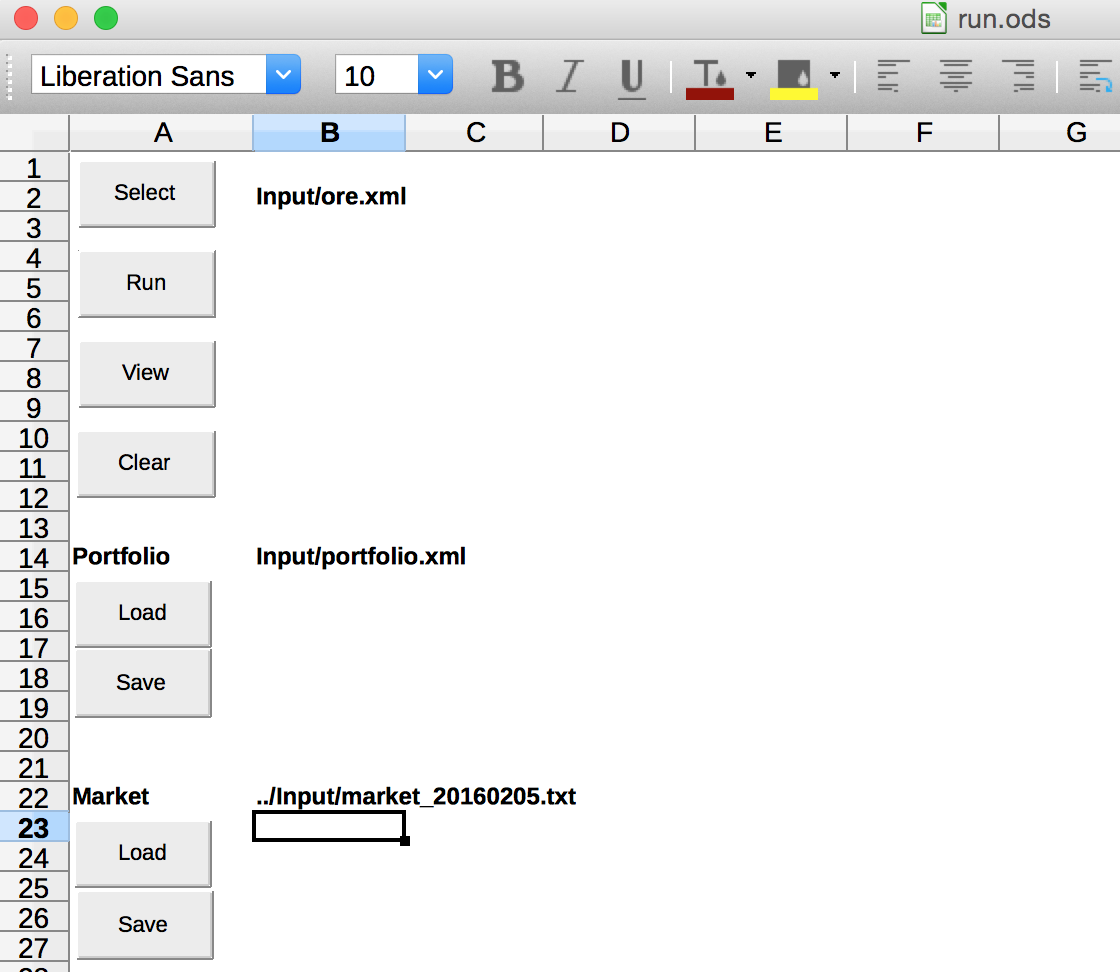
\includegraphics[scale=0.4]{demo_calc_1}
%\end{center}
%\caption{Calc sheet after launching.}
%\label{fig_14}
%\end{figure}
The user can choose a configuration (one of the {\tt ore*.xml} files in Example\_1's subfolder Input) by hitting the
'Select' button. Initially Input/ore.xml is pre-selected. The ORE process is then kicked off by hitting 'Run'. Once
completed, standard ORE reports (NPV, Cashflow, XVA) are loaded into several sheets. Moreover, exposure evolutions can
then be viewed by hitting 'View' which shows the result in figure \ref{fig_16}.  \\
\begin{figure}[h]
\begin{center}
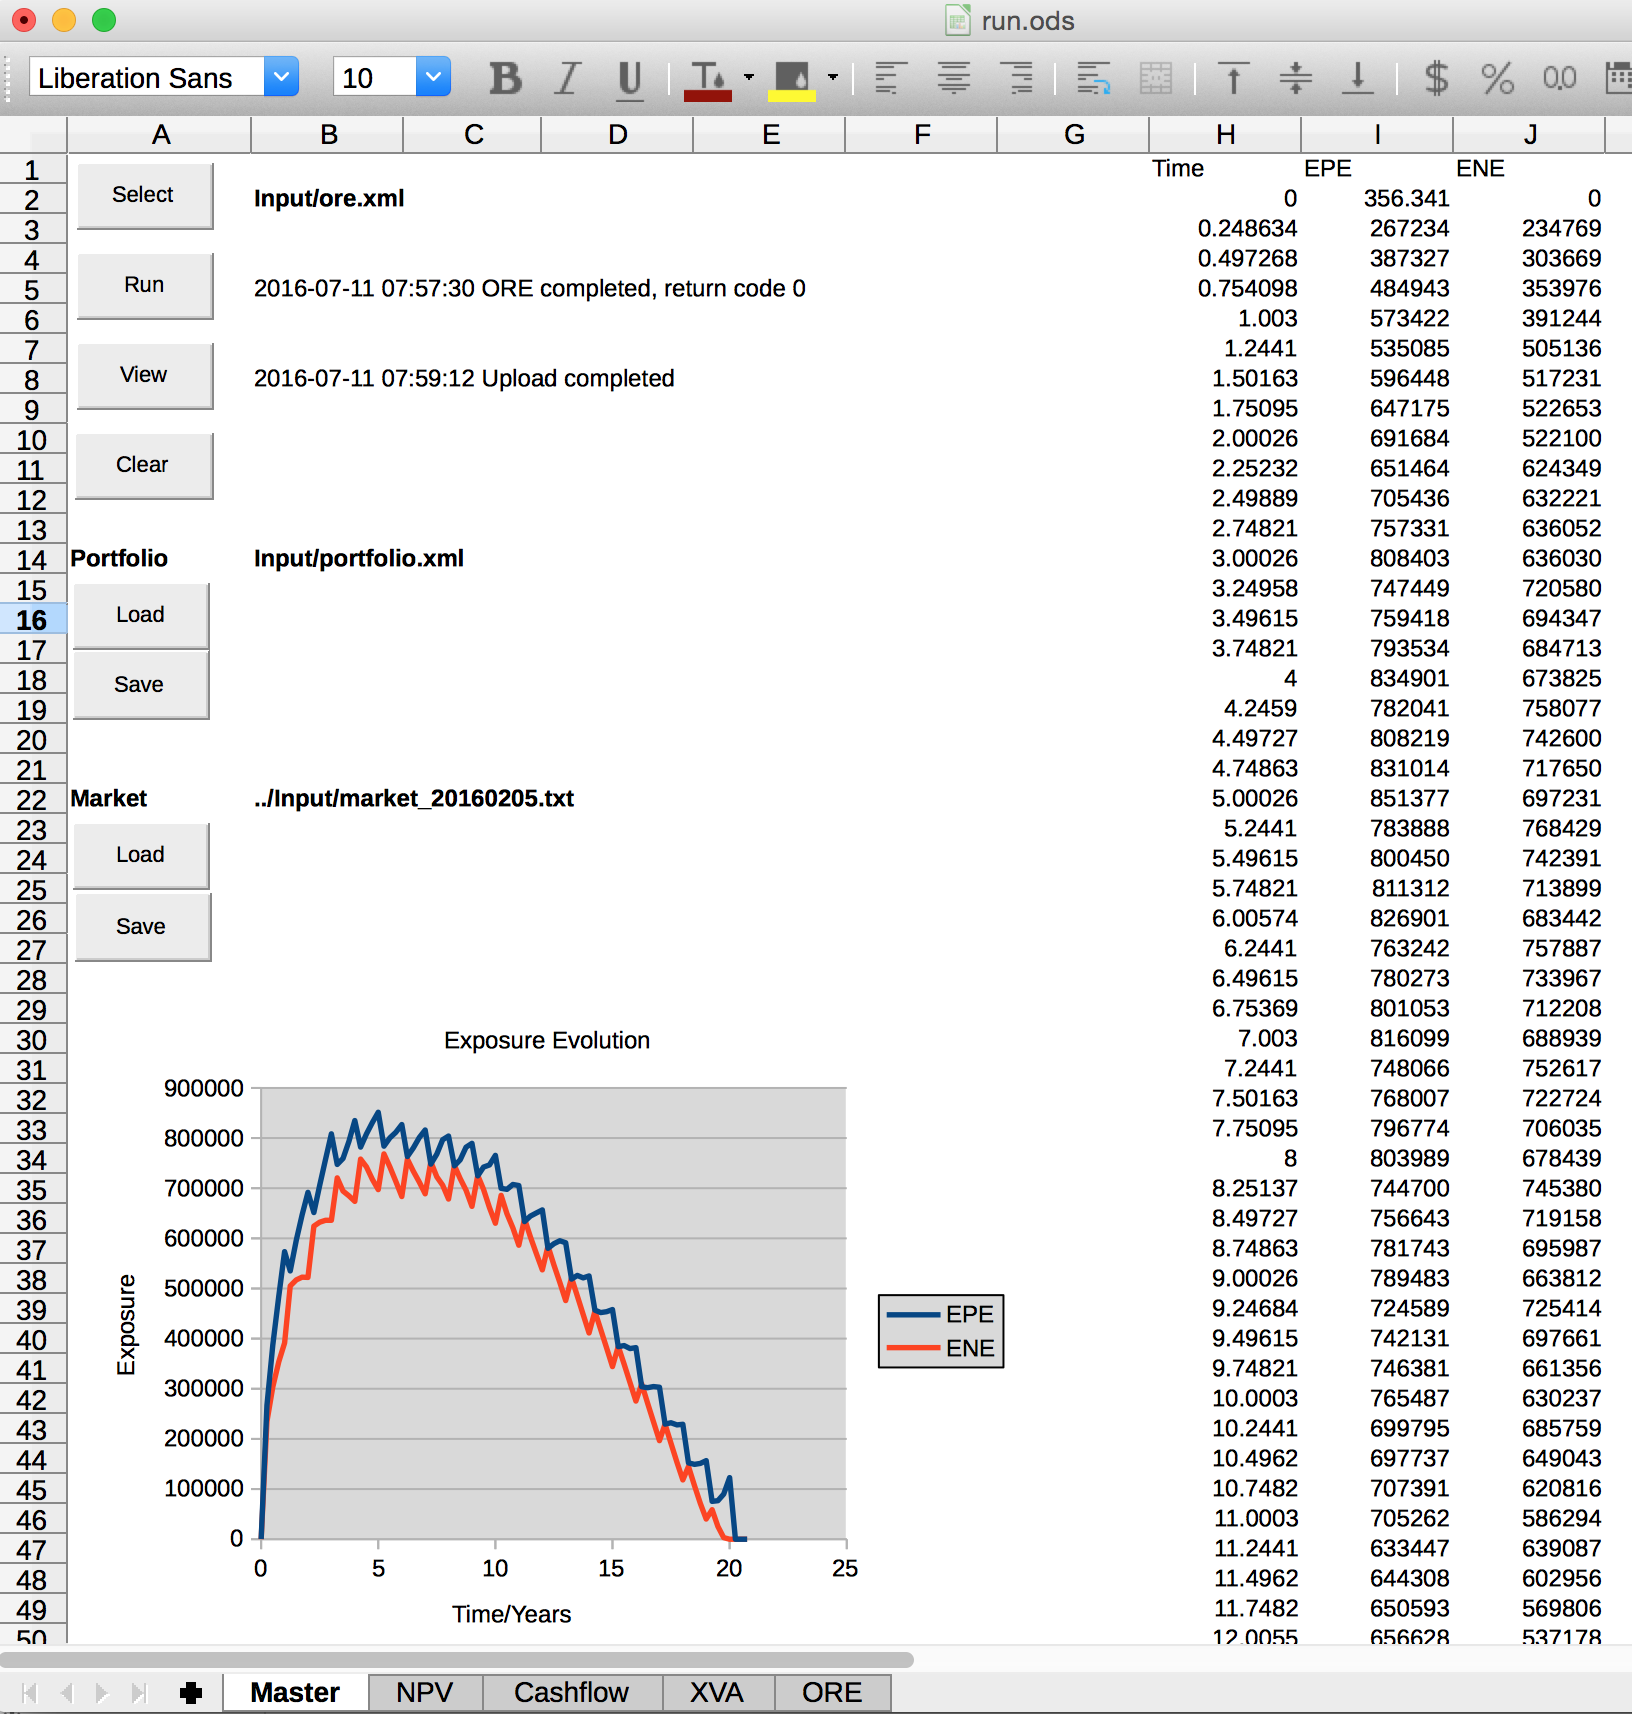
\includegraphics[scale=0.4]{demo_calc_2}
\end{center}
\caption{Calc sheet after hitting 'Run'.}
\label{fig_16}
\end{figure}

This demo uses simple Libre Office Basic macros which call Python scripts to execute ORE. The Libre Office Python uno
module (which comes with Libre Office) is used to communicate between Python and Calc to upload results into the sheets.

%\todo[inline]{Remove hard-coded file names from Python scripts}
%\todo[inline]{Calc example on Windows and Linux} 
%\todo[inline]{Harmonise layout with Excel launcher} 

\subsection{Excel}\label{sec:excel}

ORE also comes with a basic Excel sheet to demonstrate launching ORE and presenting results in Excel. This demo is more
self-contained than the Calc demo in the previous section, as it uses VBA only rather than calls to external Python
scripts. The Excel demo is available in Example\_1. Launch {\tt Example\_1.xlsm}. Then modify the paths on the first
sheet, and kick off the ORE process.

%========================================================
\section{Parameterisation}\label{sec:configuration}
%========================================================

A run of ORE is kicked off with a single command line parameter 

\medskip
\centerline{\tt ore[.exe] ore.xml}
\medskip

which points to the 'master input file' referred to  as {\tt ore.xml} subsequently. 
This file is the starting point of the engine's configuration explained in the following sub section.
An overview of all input configuration files respectively all output files is shown in Table \ref{tab_1} respectively Table \ref{tab_2}.
To set up your own ORE configuration, it might be not be necessary to start from scratch, but instead use any of the examples discussed in section \ref{sec:examples} as a boilerplate and just change the folders, see section \ref{sec:master_input}, and the trade data, see section \ref{sec:portfolio_data}, together with the netting definitions, see section \ref{sec:nettingsetinput}.

\subsection{Master Input File: {\tt ore.xml}}\label{sec:master_input}

The master input file contains general setup information (paths to configuration, trade data and market data), as well
as the selection and configuration of analytics. The file has an opening and closing root element {\tt <ORE>}, {\tt
  </ORE>} with three sections
\begin{itemize}
\item Setup
\item Logging
\item Markets
\item Analytics
\end{itemize}
which we will explain in the following.

\subsubsection{Setup}

This subset of data is easiest explained using an example, see listing \ref{lst:ore_setup}.
\begin{listing}[H]
%\hrule\medskip
\begin{minted}[fontsize=\footnotesize]{xml}
<Setup>
  <Parameter name="asofDate">2016-02-05</Parameter>
  <Parameter name="inputPath">Input</Parameter>
  <Parameter name="outputPath">Output</Parameter>
  <Parameter name="logFile">log.txt</Parameter>
  <Parameter name="logMask">255</Parameter>
  <Parameter name="marketDataFile">../../Input/market_20160205.txt</Parameter>
  <Parameter name="fixingDataFile">../../Input/fixings_20160205.txt</Parameter>
  <Parameter name="dividendDataFile">../../Input/dividends_20160205.txt</Parameter> <!-- Optional -->
  <Parameter name="implyTodaysFixings">Y</Parameter>
  <Parameter name="curveConfigFile">../../Input/curveconfig.xml</Parameter>
  <Parameter name="conventionsFile">../../Input/conventions.xml</Parameter>
  <Parameter name="marketConfigFile">../../Input/todaysmarket.xml</Parameter>
  <Parameter name="pricingEnginesFile">../../Input/pricingengine.xml</Parameter>
  <Parameter name="portfolioFile">portfolio.xml</Parameter>
  <Parameter name="calendarAdjustment">../../Input/calendaradjustment.xml</Parameter>
  <Parameter name="currencyConfiguration">../../Input/currencies.xml</Parameter>
  <Parameter name="referenceDataFile">../../Input/referencedata.xml</Parameter>
  <Parameter name="iborFallbackConfig">../../Input/iborFallbackConfig.xml</Parameter>
  <!-- None, Unregister, Defer or Disable -->
  <Parameter name="observationModel">Disable</Parameter>
  <Parameter name="lazyMarketBuilding">false</Parameter>
  <Parameter name="continueOnError">false</Parameter>
  <Parameter name="buildFailedTrades">true</Parameter>
  <Parameter name="nThreads">4</Parameter>
</Setup>
\end{minted}
%\hrule
\caption{ORE setup example}
\label{lst:ore_setup}
\end{listing}

Parameter names are self explanatory: Input and output path are interpreted relative from the directory where the ORE
executable is executed, but can also be specified using absolute paths. All file names are then interpreted relative to the
'inputPath' and 'outputPath', respectively. The files starting with {\tt ../../Input/} then point to files in the global
Example input directory {\tt Example/Input/*}, whereas files such as {\tt portfolio.xml} are local inputs in {\tt 
Example/Example\_\#/Input/}. 

Parameter {\tt logMask} determines the verbosity of log file output. Log messages are 
internally labelled as Alert, Critical, Error, Warning, Notice, Debug, associated with logMask values 1, 2, 4, 8, ..., 64. 
The logMask allows filtering subsets of these categories and controlling the verbosity of log file output\footnote{by bitwise comparison of the the external logMask value with each message's log level}. LogMask 255 ensures maximum verbosity. \\

When ORE starts, it will initialise today's market, i.e. load market data, fixings and dividends, and build all term
structures as specified in {\tt todaysmarket.xml}.  Moreover, ORE will load the trades in {\tt portfolio.xml} and link
them with pricing engines as specified in {\tt pricingengine.xml}. When parameter {\tt implyTodaysFixings} is set to Y,
today's fixings would not be loaded but implied, relevant when pricing/bootstrapping off hypothetical market data as
e.g. in scenario analysis and stress testing. The curveConfigFile {\tt curveconfig.xml}, the conventionsFile {\tt
  conventions.xml}, the referenceDataFile {\tt referencedata.xml}, the iborFallbackConfig, the marketDataFile and the
fixingDataFile are explained in the sections below.

\medskip Parameter {\tt calendarAdjustment} includes the {\tt calendarAdjustment.xml} which lists out additional holidays and
business days to be added to specified calendars.

\medskip The optional parameter {\tt currencyConfiguration} points to a configuration file that contains additional currencies
to be added to ORE's setup, see {\tt Examples/Input/currencies.xml} for a full list of ISO currencies and a few unofficial currency
codes that can thus be made available in ORE. Note that the external configuration does not override any currencies that are
hard-coded in the QuantLib/QuantExt libraries, only currencies not present already are added from the external configuration file.

\medskip The last parameter {\tt observationModel} can be used to control ORE performance during simulation. The choices
{\em Disable } and {\em Unregister } yield similarly improved performance relative to choice {\em None}. For users
familiar with the QuantLib design - the parameter controls to which extent {\em QuantLib observer notifications} are
used when market and fixing data is updated and the evaluation date is shifted:
\begin{itemize}
\item The 'Unregister' option limits the amount of notifications by unregistering floating rate coupons from indices;
\item Option 'Defer' disables all notifications during market data and fixing updates with
{\tt ObservableSettings::instance().disableUpdates(true)}
and kicks off updates afterwards when enabled again
\item The 'Disable' option goes one step further and disables all notifications during market data and fixing updates,
  and in particular when the evaluation date is changed along a path, with \\
  {\tt ObservableSettings::instance().disableUpdates(false)} \\
  Updates are not deferred here. Required term structure and instrument recalculations are triggered explicitly.
\end{itemize}
%\todo[inline]{Expand the technical description of observationModel}

\medskip If the parameter {\tt lazyMarketBuilding} is set to true, the build of the curves in the TodaysMarket is
delayed until they are actually requested. This can speed up the processing when some curves configured in TodaysMarket
are not used. If not given, the parameter defaults to {\tt true}.

\medskip If the parameter {\tt continueOnError} is set to true, the application will not exit on an error, but try to
continue the processing. If not given, the parameter defaults to {\tt false}.

\medskip If the parameter {\tt buildFailedTrades} is set to true, the application will build a dummy trade if loading or
building the original trade fails. The dummy trade has trade type ``Failed'', zero notional and NPV.
If not given, the parameter defaults to {\tt false}.

\medskip If the parameter {\tt nThreads} is given, multiple threads will be used for valuation engine runs where
applicable (Sensitivity, Exposure Classic, Exposure AMC). If not given, the parameter defaults to $1$.

\subsubsection{Logging}\label{sec:master_input_logging}

The {\tt Logging} section (see listing \ref{lst:ore_logging}) is used to configure some ORE logging options.

\begin{listing}[H]
%\hrule\medskip
\begin{minted}[fontsize=\footnotesize]{xml}
<Logging>
  <Parameter name="logFile">log.txt</Parameter>
  <Parameter name="logMask">31</Parameter>
  <Parameter name="progressLogFile">my_log_progress_%N.json</Parameter>
  <Parameter name="progressLogRotationSize">102400</Parameter>
  <Parameter name="progressLogToConsole">false</Parameter>
  <Parameter name="structuredLogFile">my_structured_logs_%N.txt</Parameter>
  <Parameter name="structuredLogRotationSize">102400</Parameter>
</Logging>
\end{minted}
%\hrule
\caption{ORE logging}
\label{lst:ore_logging}
\end{listing}

Parameter {\tt logFile} and {\tt logMask} will override the same parameters in the {\tt Setup} section.

Parameters {\tt progressLogFile} and {\tt structuredLogFile} are the filename where progress log messages
and structured log messages are written out to, respectively, which supports Boost string patterns.This defaults to ``log\_progress\_\%N.json'' and ``log\_structured\_\%N.json'', respectively, where {\tt N} will be an integer (beginning at 0) used for log file rotation.

Parameters {\tt progressLogRotationSize} and {\tt structuredLogRotationSize} are the size limit (in bytes)
of each log file before applying log file rotation to the progress log file and structured log message file,
respectively.. For example, $10 * 1024 * 1024 = 10 \text{MiB}$. Defaults to 100 MiB.

If the parameter {\tt progressLogToConsole} is set to true, then progress logs will be written to std::cout.
This can be used simultaneously with {\tt progressLogFile}, i.e.\ progress logs can be written out
to both file and std::cout.

\subsubsection{Markets}\label{sec:master_input_markets}

The {\tt Markets} section (see listing \ref{lst:ore_markets}) is used to choose market configurations for calibrating
the IR, FX and EQ simulation model components, pricing and simulation, respectively. These configurations have to be 
defined
in {\tt todaysmarket.xml} (see section \ref{sec:market}).

\begin{listing}[H]
%\hrule\medskip
\begin{minted}[fontsize=\footnotesize]{xml}
<Markets>
  <Parameter name="lgmcalibration">collateral_inccy</Parameter>
  <Parameter name="fxcalibration">collateral_eur</Parameter>
  <Parameter name="eqcalibration">collateral_inccy</Parameter>
  <Parameter name="pricing">collateral_eur</Parameter>
  <Parameter name="simulation">collateral_eur</Parameter>
</Markets>
\end{minted}
%\hrule
\caption{ORE markets}
\label{lst:ore_markets}
\end{listing}

For example, the calibration of the simulation model's interest rate components requires local OIS discounting whereas
the simulation phase requires cross currency adjusted discount curves to get FX product pricing right. So far, the
market configurations are used only to distinguish discount curve sets, but the market configuration concept in ORE
applies to all term structure types.

\subsubsection{Analytics}\label{sec:analytics}

The {\tt Analytics} section lists all permissible analytics using tags {\tt <Analytic type="..."> ... </Analytic>} where
type can be (so far) in
\begin{itemize}
\item npv
\item cashflow
\item curves
\item simulation
\item xva
\item sensitivity
\item stress
\item parametricVar
\item simm
\end{itemize}

Each {\tt Analytic} section contains a list of key/value pairs to parameterise the analysis of the form {\tt <Parameter
  name="key">value</Parameter>}. Each analysis must have one key {\tt active} set to Y or N to activate/deactivate this
analysis.  The following listing \ref{lst:ore_analytics} shows the parametrisation of the first four basic analytics in
the list above.

\begin{listing}[H]
%\hrule\medskip
\begin{minted}[fontsize=\footnotesize]{xml}
<Analytics>    
  <Analytic type="npv">
    <Parameter name="active">Y</Parameter>
    <Parameter name="baseCurrency">EUR</Parameter>
    <Parameter name="outputFileName">npv.csv</Parameter>
    <Parameter name="additionalResults">Y</Parameter>
  </Analytic>      
  <Analytic type="cashflow">
    <Parameter name="active">Y</Parameter>
    <Parameter name="outputFileName">flows.csv</Parameter>
    <Parameter name="includePastCashflows">N</Parameter>
  </Analytic>      
  <Analytic type="curves">
    <Parameter name="active">Y</Parameter>
    <Parameter name="configuration">default</Parameter>
    <Parameter name="grid">240,1M</Parameter>
    <Parameter name="outputFileName">curves.csv</Parameter>
    <Parameter name="outputTodaysMarketCalibration">N</Parameter>
  </Analytic>
  <Analytic type="...">
    <!-- ... -->
  </Analytic>      
</Analytics>      
\end{minted}
\caption{ORE analytics: npv, cashflow, curves, additional results, todays market calibration}
\label{lst:ore_analytics}
\end{listing}

The cashflow analytic writes a report containing all future cashflows of the portfolio. Table \ref{cashflowreport} shows
a typical output for a vanilla swap.

\begin{table}[hbt]
\scriptsize
\begin{center}
  \begin{tabular}{l|l|l|l|r|l|r|r|l|r|r}
\hline
\#ID & Type & LegNo & PayDate & Amount & Currency & Coupon & Accrual & fixingDate & fixingValue & Notional \\
\hline
\hline
tr123 & Swap & 0 & 13/03/17 & -111273.76 & EUR & -0.00201 & 0.50556 & 08/09/16 & -0.00201 & 100000000.00 \\
tr123 & Swap & 0 & 12/09/17 & -120931.71 & EUR & -0.002379 & 0.50833 & 09/03/17 & -0.002381 & 100000000.00 \\
\ldots
\end{tabular}
\caption{Cashflow Report}
\label{cashflowreport}
\end{center}
\end{table}

The amount column contains the projected amount including embedded caps and floors and convexity (if applicable), the
coupon column displays the corresponding rate estimation. The fixing value on the other hand is the plain fixing
projection as given by the forward value, i.e. without embedded caps and floors or convexity.

Note that the fixing value might deviate from the coupon value even for a vanilla coupon, if the QuantLib library was
compiled {\em without} the flag \verb+QL_USE_INDEXED_COUPON+ (which is the default case). In this case the coupon value
uses a par approximation for the forward rate assuming the index estimation period to be identical to the accrual
period, while the fixing value is the actual forward rate for the index estimation period, i.e. whenever the index estimation
period differs from the accrual period the values will be slightly different.

The Notional column contains the underlying notional used to compute the amount of each coupon. It contains \verb+#NA+
if a payment is not a coupon payment.

The curves analytic exports all yield curves that have been built according to the specification in {\tt
  todaysmarket.xml}. Key {\tt configuration} selects the curve set to be used (see explanation in the previous Markets
section).  Key {\tt grid} defines the time grid on which the yield curves are evaluated, in the example above a grid of
240 monthly time steps from today. The discount factors for all curves with configuration default will be exported on
this monthly grid into the csv file specified by key {\tt outputFileName}. The grid can also be specified explicitly by
a comma separated list of tenor points such as {\tt 1W, 1M, 2M, 3M, \dots}.

The additionalResults analytic writes a report containing any additional results generated for the portfolio. The results are pricing engine specific but Table \ref{additionalreport} shows the output for a vanilla swaption.

\begin{table}[hbt]
\scriptsize
\begin{center}
  \begin{tabular}{l|l|l|l}
\hline
\#TradeId & ResultId & ResultType & ResultValue \\
example\_swaption & annuity & double & 2123720984 \\
example\_swaption & atmForward & double & 0.01664135 \\
example\_swaption & spreadCorrection & double & 0 \\
example\_swaption & stdDev & double & 0.00546015 \\
example\_swaption & strike & double & 0.024 \\
example\_swaption & swapLength & double & 4 \\
example\_swaption & vega & double & 309237709.5 \\
\hline
\hline
\ldots
\end{tabular}
\caption{AdditionalResults Report}
\label{additionalreport}
\end{center}
\end{table}

The todaysMarketCalibration analytic writes a report containing information on the build of the t0 market.

\medskip The purpose of the {\tt simulation} 'analytics' is to run a Monte Carlo simulation which evolves the market as
specified in the simulation config file. The primary result is an NPV cube file, i.e. valuations of all trades in the
portfolio file (see section Setup), for all future points in time on the simulation grid and for all paths. Apart from
the NPV cube, additional scenario data (such as simulated overnight rates etc) are stored in this process which are
needed for subsequent XVA analytics.

\begin{listing}[H]
%\hrule\medskip
\begin{minted}[fontsize=\footnotesize]{xml}
<Analytics>
  <Analytic type="simulation">
    <Parameter name="active">Y</Parameter>
    <Parameter name="simulationConfigFile">simulation.xml</Parameter>
    <Parameter name="pricingEnginesFile">../../Input/pricingengine.xml</Parameter>
    <Parameter name="baseCurrency">EUR</Parameter>
    <Parameter name="storeFlows">Y</Parameter>
    <Parameter name="storeSurvivalProbabilities">Y</Parameter>
    <Parameter name="cubeFile">cube_A.csv.gz</Parameter>
    <Parameter name="nettingSetCubeFile">nettingSetCube_A.csv.gz</Parameter>
    <Parameter name="cptyCubeFile">cptyCube_A.csv.gz</Parameter>
    <Parameter name="aggregationScenarioDataFileName">scenariodata.csv.gz</Parameter>
    <Parameter name="aggregationScenarioDump">scenariodump.csv</Parameter>
  </Analytic>
</Analytics>      
\end{minted}
\caption{ORE analytic: simulation}
\label{lst:ore_simulation}
\end{listing}

The pricing engines file specifies how trades are priced under future scenarios which can differ from pricing as of
today (specified in section Setup).  Key base currency determines into which currency all NPVs will be converted. Key
store scenarios (Y or N) determines whether the market scenarios are written to a file for later reuse. Key
`store flows' (Y or N) controls whether cumulative cash flows between simulation dates are stored in the (hyper-)
cube for post processing in the context of Dynamic Initial Margin and Variation Margin calculations. And finally, the
key `store survival probabilities' (Y or N) controls whether survival probabilities on simulation dates are stored in the
cube for post processing in the context of Dynamic Credit XVA calculation. The additional
scenario data (written to the specified file here) is likewise required in the post processor step. These data comprise
simulated index fixing e.g. for collateral compounding and simulated FX rates for cash collateral conversion into base
currency. The scenario dump file, if specified here, causes ORE to write simulated market data to a human-readable csv
file. Only those currencies or indices are written here that are stated in the AggregationScenarioDataCurrencies and 
AggregationScenarioDataIndices subsections of the simulation files market section, see also section
\ref{sec:sim_market}.
 
\medskip The XVA analytic section offers CVA, DVA, FVA and COLVA calculations which can be selected/deselected here
individually. All XVA calculations depend on a previously generated NPV cube (see above) which is referenced here via
the {\tt cubeFile} parameter. This means one can re-run the XVA analytics without regenerating the cube each time. The
XVA reports depend in particular on the settings in the {\tt csaFile} which determines CSA details such as margining
frequency, collateral thresholds, minimum transfer amounts, margin period of risk. By splitting the processing into
pre-processing (cube generation) and post-processing (aggregation and XVA analysis) it is possible to vary these CSA
details and analyse their impact on XVAs quickly without re-generating the NPV cube. The cube file is usually a
compressed csv file (using gzip compression, with file ending .csv.gz), except when the file extension is set explicitly
to txt or csv in which case an uncompressed version of the file is written to disk.

\begin{listing}[H]
%\hrule\medskip
\begin{minted}[fontsize=\footnotesize]{xml}
<Analytics>
  <Analytic type="xva">
    <Parameter name="active">Y</Parameter>
    <Parameter name="csaFile">netting.xml</Parameter>
    <Parameter name="cubeFile">cube.csv.gz</Parameter>
    <Parameter name="scenarioFile">scenariodata.csv.gz</Parameter>
    <Parameter name="baseCurrency">EUR</Parameter>
    <Parameter name="exposureProfiles">Y</Parameter>
    <Parameter name="exposureProfilesByTrade">Y</Parameter>
    <Parameter name="quantile">0.95</Parameter>
    <Parameter name="calculationType">NoLag</Parameter>      
    <Parameter name="allocationMethod">None</Parameter>    
    <Parameter name="marginalAllocationLimit">1.0</Parameter>
    <Parameter name="exerciseNextBreak">N</Parameter>
    <Parameter name="cva">Y</Parameter>
    <Parameter name="dva">N</Parameter>
    <Parameter name="dvaName">BANK</Parameter>
    <Parameter name="fva">N</Parameter>
    <Parameter name="fvaBorrowingCurve">BANK_EUR_BORROW</Parameter>
    <Parameter name="fvaLendingCurve">BANK_EUR_LEND</Parameter>
    <Parameter name="colva">Y</Parameter>
    <Parameter name="collateralFloor">Y</Parameter>
    <Parameter name="dynamicCredit">N</Parameter>
    <Parameter name="kva">Y</Parameter>
    <Parameter name="kvaCapitalDiscountRate">0.10</Parameter>
    <Parameter name="kvaAlpha">1.4</Parameter>
    <Parameter name="kvaRegAdjustment">12.5</Parameter>
    <Parameter name="kvaCapitalHurdle">0.012</Parameter>
    <Parameter name="kvaOurPdFloor">0.03</Parameter>
    <Parameter name="kvaTheirPdFloor">0.03</Parameter>
    <Parameter name="kvaOurCvaRiskWeight">0.005</Parameter>
    <Parameter name="kvaTheirCvaRiskWeight">0.05</Parameter>
    <Parameter name="dim">Y</Parameter>
    <Parameter name="mva">Y</Parameter>
    <Parameter name="dimQuantile">0.99</Parameter>
    <Parameter name="dimHorizonCalendarDays">14</Parameter>
    <Parameter name="dimRegressionOrder">1</Parameter>
    <Parameter name="dimRegressors">EUR-EURIBOR-3M,USD-LIBOR-3M,USD</Parameter>
    <Parameter name="dimLocalRegressionEvaluations">100</Parameter>
    <Parameter name="dimLocalRegressionBandwidth">0.25</Parameter>
    <Parameter name="dimScaling">1.0</Parameter>
    <Parameter name="dimEvolutionFile">dim_evolution.txt</Parameter>
    <Parameter name="dimRegressionFiles">dim_regression.txt</Parameter>
    <Parameter name="dimOutputNettingSet">CPTY_A</Parameter>      
    <Parameter name="dimOutputGridPoints">0</Parameter>
    <Parameter name="rawCubeOutputFile">rawcube.csv</Parameter>
    <Parameter name="netCubeOutputFile">netcube.csv</Parameter>
    <Parameter name="fullInitialCollateralisation">true</Parameter>
    <Parameter name="flipViewXVA">N</Parameter>
    <Parameter name="flipViewBorrowingCurvePostfix">_BORROW</Parameter>
    <Parameter name="flipViewLendingCurvePostfix">_LEND</Parameter>
  </Analytic>
</Analytics>
\end{minted}
\caption{ORE analytic: xva}
\label{lst:ore_xva}
\end{listing}

Parameters:
\begin{itemize}
\item {\tt csaFile:} Netting set definitions file covering CSA details such as margining frequency, thresholds, minimum
transfer amounts, margin period of risk
\item {\tt cubeFile:} NPV cube file previously generated and to be post-processed here
\item {\tt scenarioFile:} Scenario data previously generated and used in the post-processor (simulated index fixings and
FX rates)
\item {\tt baseCurrency:} Expression currency for all NPVs, value adjustments, exposures
\item {\tt exposureProfiles:} Flag to enable/disable exposure output for each netting set
\item {\tt exposureProfilesByTrade:} Flag to enable/disable stand-alone exposure output for each trade
\item {\tt quantile:} Confidence level for Potential Future Exposure (PFE) reporting
\item {\tt calculationType:} Determines the settlement of margin calls. The admissible choices depend on having a close-out grid, see table \ref{tab:calcTypes}; \\
	\begin{itemize}
		\item if there isn't any ``close-out'' grid -see section \ref{sec:simulation}-, the choices are:
		\begin{itemize}
			\item {\em Symmetric} - margin for both counterparties settled after the margin period of risk;
			\item {\em AsymmetricCVA} - margin requested from the counterparty settles with delay,
			margin requested from us settles immediately;
			\item {\em AsymmetricDVA} - vice versa.
		\end{itemize}
		\item If there is a ``close-out'' grid -see section \ref{sec:simulation}-, only choice is:
		\begin{itemize}
			\item {\em NoLag} - used to disable any delayed settlement of the margin. 
		\end{itemize}
	\end{itemize}
	\todo[inline]{Move calculationType into the {\tt csaFile}?}
%
NoLag is the default configuration.
%
\begin{table}[!h]
\centering
\arrayrulecolor{black}
\begin{tabular}{!{\color{black}\vrule}c!{\color{black}\vrule}c!{\color{black}\vrule}l!{\color{black}\vrule}} 
\hline
\multicolumn{1}{!{\color{black}\vrule}l!{\color{black}\vrule}}{Grid Type} & \multicolumn{1}{l!{\color{black}\vrule}}{{\tt calculationType}} & Comment                                                                                                                                                                                           \\ 
\hline
\multirow{4}{*}{without close-out grid}                                    & {\em NoLag}                                                      & Not Supported                                                                                                                                                                                     \\ 
\cline{2-3}
                                                                          & {\em Symmetric}                                                  & Supported\tablefootnote{\label{note1} The calculations are correct only if the simulation grid (see section \ref{sec:simulation}) is equally-spaced with time steps that match the MPoR defined in netting-set definition (see section \ref{sec:CollNettingSet}). See section \ref{sec:mpor} for further explanation.}  \\ 
\cline{2-3}
                                                                          & {\em AsymmetricCVA}                                              & Supported \footref{note1} \\ 
\cline{2-3}
                                                                          & {\em AsymmetricDVA}                                              & Supported \footref{note1}\\ 
\hline
\multirow{4}{*}{with close-out grid}                                       & {\em NoLag}                                                      & Supported\tablefootnote{Close-out lag (see section \ref{sec:simulation}) must be equal to MPoR defined in netting-set definition (see section \ref{sec:CollNettingSet}). Otherwise, an error will be thrown.}                                           \\ 
\cline{2-3}
                                                                          & {\em Symmetric}                                                  & Not Supported                                                                                                                                                                                     \\ 
\cline{2-3}
                                                                          & {\em AsymmetricCVA}                                              & Not Supported                                                                                                                                                                                     \\ 
\cline{2-3}
                                                                          & {\em AsymmetricDVA}                                              & Not Supported                                                                                                                                                                                     \\
\hline
\end{tabular}
\arrayrulecolor{black}
\caption{Overview of admissible calculation types with combination of grid types.} \label{tab:calcTypes}
\end{table}
%
\item {\tt allocationMethod:} XVA allocation method, choices are {\em None, Marginal, RelativeXVA, RelativeFairValueGross, RelativeFairValueNet}
\item {\tt marginalAllocationLimit:} The marginal allocation method a la Pykhtin/Rosen breaks down when the netting set
value vanishes while the exposure does not. This parameter acts as a cutoff for the marginal allocation when the
absolute netting set value falls below this limit and switches to equal distribution of the exposure in this case.
\item {\tt exerciseNextBreak:} Flag to terminate all trades at their next break date before aggregation and the
subsequent analytics
\item {\tt cva, dva, fva, colva, collateralFloor, dim, mva:} Flags to enable/disable these analytics. \todo[inline]{Add
collateral rates floor to the collateral model file (netting.xml)}
\item {\tt dvaName:} Credit name to look up the own default probability curve and recovery rate for DVA calculation
\item {\tt fvaBorrowingCurve:} Identifier of the borrowing yield curve
\item {\tt fvaLendingCurve:} Identifier of the lending yield curve
%\item {\tt collateralSpread:} Deviation between collateral rate and overnight rate, expressed in absolute terms (one
%basis point is 0.0001) assuming the day count convention of the
%collateral rate. 
%basis point is 0.0001) assuming the day count convention of the collateral rate.
\item {\tt dynamicCredit:} Flag to enable using pathwise survival probabilities when calculating CVA, DVA, FVA and MVA increments from exposures. If set to N the survival probabilities are extracted from T0 curves.
\item {\tt kva:} Flag to enable setting the kva ccr parameters.
\item {\tt kvaCapitalDiscountRate, kvaAlpha, kvaRegAdjustment, kvaCapitalHurdle, kvaOurPdFloor, kvaTheirPdFloor kvaOurCvaRiskWeight, kvaTheirCvaRiskWeight:} the kva CCR parameters (see \ref{sec:app_kva} and \ref{sec:app_kva_cva}.
\item {\tt dimQuantile:} Quantile for Dynamic Initial Margin (DIM) calculation
\item {\tt dimHorizonCalendarDays:} Horizon for DIM calculation, 14 calendar days for 2 weeks, etc.
\item {\tt dimRegressionOrder:} Order of the regression polynomial (netting set clean NPV move over the simulation
period versus netting set NPV at period start)
\item {\tt dimRegressors:} Variables used as regressors in a single- or multi-dimensional regression; these variable
  names need to match entries in the {\tt simulation.xml}'s AggregationScenarioDataCurrencies and
  AggregationScenarioDataIndices sections (only these scenario data are passed on to the post processor); if the list is
  empty, the NPV will be used as a single regressor
\item {\tt dimLocalRegressionEvaluations:} Nadaraya-Watson local regression evaluated at the given number of points to
validate polynomial regression. Note that Nadaraya-Watson needs a large number of samples for meaningful
results. Evaluating the local regression at many points (samples) has a significant performance impact, hence the option
here to limit the number of evaluations.
\item {\tt dimLocalRegressionBandwidth:} Nadaraya-Watson local regression bandwidth in standard deviations of the
independent variable (NPV)
\item {\tt dimScaling:} Scaling factor applied to all DIM values used, e.g. to reconcile simulated DIM with actual IM at
$t_0$
\item {\tt dimEvolutionFile:} Output file name to store the evolution of zero order DIM and average of nth order DIM
through time
\item {\tt dimRegressionFiles:} Output file name(s) for a DIM regression snapshot, comma separated list
\item {\tt dimOutputNettingSet:} Netting set for the DIM regression snapshot
\item {\tt dimOutputGridPoints:} Grid point(s) (in time) for the DIM regression snapshot, comma separated list
\item {\tt rawCubeOutputFile:} File name for the trade NPV cube in human readable csv file format (per trade, date,
sample), leave empty to skip generation of this file.
\item {\tt netCubeOutputFile:} File name for the aggregated NPV cube in human readable csv file format (per netting set,
date, sample) {\em after} taking collateral into account. Leave empty to skip generation of this file.
\item {\tt fullInitialCollateralisation:} If set to {\tt true}, then for every netting set, the collateral balance at $t=0$ will be set to the NPV of the setting set. The resulting effect is that EPE, ENE and PFE are all zero at $t=0$. If set to {\tt false} (default value), then the collateral balance at $t=0$ will be set to zero.
\item {\tt flipViewXVA:} If set to {\tt Y}, the perspective in XVA calculations is switched to the cpty view, the npvs and the netting sets being reverted during calculation. In order to get the lending/borrowing curve, the calculation assumes these curves being set up with the cptyname + the postfix given in the next two settings.
\item {\tt flipViewBorrowingCurvePostfix:} postfix for the borrowing curve, the calculation assumes this is curves being set up with cptyname + postfix given.
\item {\tt flipViewLendingCurvePostfix:} postfix for the lending curve, the calculation assumes this is curve being set up with cptyname + postfix given.
\end{itemize}

The two cube file outputs {\tt rawCubeOutputFile} and {\tt netCubeOutputFile} are provided for interactive analysis and visualisation purposes, see section
\ref{sec:visualisation}.

\medskip The {\tt sensitivity} and {\tt stress} 'analytics' provide computation of bump and revalue (zero rate
resp. optionlet) sensitivities and NPV changes under user defined stress scenarios. Listing \ref{lst:ore_sensitivity}
shows a typical configuration for sensitivity calculation.

\begin{listing}[H]
%\hrule\medskip
\begin{minted}[fontsize=\footnotesize]{xml}
<Analytics>
 <Analytic type="sensitivity">
   <Parameter name="active">Y</Parameter>
   <Parameter name="marketConfigFile">simulation.xml</Parameter>
   <Parameter name="sensitivityConfigFile">sensitivity.xml</Parameter>
   <Parameter name="pricingEnginesFile">../../Input/pricingengine.xml</Parameter>
   <Parameter name="scenarioOutputFile">scenario.csv</Parameter>
   <Parameter name="sensitivityOutputFile">sensitivity.csv</Parameter>
   <Parameter name="crossGammaOutputFile">crossgamma.csv</Parameter>
   <Parameter name="outputSensitivityThreshold">0.000001</Parameter>
   <Parameter name="recalibrateModels">Y</Parameter>
   <!-- Additional parametrisation for par sensitivity analysis -->
   <Parameter name="parSensitivity">Y</Parameter>
   <Parameter name="parSensitivityOutputFile">parsensitivity.csv</Parameter>
   <Parameter name="outputJacobi">Y</Parameter>
   <Parameter name="jacobiOutputFile">jacobi.csv</Parameter>
   <Parameter name="jacobiInverseOutputFile">jacobi_inverse.csv</Parameter>
 </Analytic>
</Analytics>
\end{minted}
\caption{ORE analytic: sensitivity}
\label{lst:ore_sensitivity}
\end{listing}
%   <Parameter name="parRateSensitivityOutputFile">parsensi.csv</Parameter>

The parameters have the following interpretation:

\begin{itemize}
\item {\tt marketConfigFile:} Configuration file defining the simulation market under which sensitivities are computed,
  see \ref{sec:simulation}. Only a subset of the specification is needed (the one given under {\tt Market}, see
  \ref{sec:sim_market} for a detailed description).
\item {\tt sensitivityConfigFile:} Configuration file  for the sensitivity calculation, see section \ref{sec:sensitivity}.
\item {\tt pricingEnginesFile:} Configuration file for the pricing engines to be used for sensitivity calculation.
\item {\tt scenarioOutputFile:} File containing the results of the sensitivity calculation in terms of the base scenario
  NPV, the scenario NPV and their difference.
\item {\tt sensitivityOutputFile:} File containing the results of the sensitivity calculation in terms of the base scenario
  NPV, the shift size together with the risk-factor and the resulting first and (pure) second order finite differences.
  Also included is a second set of shift sizes together with the risk-factor with a (mixed) second order finite difference associated to a cross gamma calculation
%\item {\tt parRateSensitivityOutputFile:} File containing par sensitivities (only available in ORE+)
\item {\tt outputSensitivityThreshold:} Only finite differences with absolute value greater than this number are written
  to the output files.
\item {\tt recalibrateModels:} If set to Y, then recalibrate pricing models after each shift of relevant term structures; otherwise do not recalibrate
\item {\tt parSensitivity}: If set to Y, par sensitivity analysis is performed following the "raw" sensitivity analysis; note that in this case the 
{\tt sensitivityConfigFile} needs to contain {\tt ParConversion} sections, see {\tt Example\_40}   
\item {\tt parSensitivityOutputFile}: Output file name for the par sensitivity report
\item {\tt outputJacobi}: If set to Y, then the relevant Jacobi and inverse Jacobi matrix is written to a file, see below
\item {\tt jacobiOutputFile}: Output file name for the Jacobi matrx
\item {\tt jacobiInverseOutputFile}: Output file name for the inverse Jacobi matrix
\end{itemize}


The zero to par sensitivity conversion analytics configuration is similar to the one of the sensitivity calculation. Listing \ref{lst:ore_zerotoparconversion}
shows an example.

\begin{listing}[H]
%\hrule\medskip
\begin{minted}[fontsize=\footnotesize]{xml}
<Analytics>
 <Analytic type="zeroToParSensiConversion">
      <Parameter name="active">Y</Parameter>
      <Parameter name="marketConfigFile">simulation.xml</Parameter>
      <Parameter name="sensitivityConfigFile">sensitivity.xml</Parameter>
      <Parameter name="pricingEnginesFile">../../Input/pricingengine.xml</Parameter>
      <Parameter name="sensitivityInputFile">sensitivity.csv</Parameter>
      <Parameter name="outputThreshold">0.000001</Parameter>
      <Parameter name="outputFile">parconversion_sensitivity.csv</Parameter>
      <Parameter name="outputJacobi">Y</Parameter>
      <Parameter name="jacobiOutputFile">jacobi.csv</Parameter>
      <Parameter name="jacobiInverseOutputFile">jacobi_inverse.csv</Parameter>
    </Analytic>
</Analytics>
\end{minted}
\caption{ORE analytic: Zero to Par Sensitivity Conversion}
\label{lst:ore_zerotoparconversion}
\end{listing}

The parameters have the same interpretation as for the sensitivity analytic. There is one new parameter *sensitivityInputFile* which points to a csv file with the raw (zero)sensitivites. Those raw sensitivites will be converted into par sensitivities, using the the same methodology described in \ref{app:par_sensi} and the configuration is described in \ref{sec:sensitivity}.

The raw sensitivites csv input file *sensitivityInputFile* needs to have at least six columns, the column names can be user configured in the master input file. Here is a description of each of the columns:

\begin{enumerate}
\item idColumn : Column with a unique identifier for the trade / nettingset / portfolio.
\item riskFactorColumn: Column with the identifier of the zero/raw sensitiviy. The risk factor name needs to follow the ORE naming convention, e.g. DiscountCurve/EUR/5/1Y (the 6th bucket in EUR discount curve as specified in the sensitivity.xml)\
\item deltaColumn: The raw sensitivity of the trade/nettingset / portfolio with respect to the risk factor
\item currencyColumn: The currency in which the raw sensitivity is expressed, need to be the same as the BaseCurrency in the simulation settings.
\item shiftSizeColumn: The shift size applied to compute the raw sensitivity, need to be consistent to the sensitivity configuration.
\item baseNpvColumn: The base npv of the trade / nettingset / portfolio in currency.
\end{enumerate}

Here is an example for an input file:

\begin{table}[hbt]
\scriptsize
\begin{center}
\begin{tabular}{lllrlrr}
\hline
{} & \#TradeId &                Factor\_1 &  ShiftSize\_1 & Currency &  Base NPV &  Delta \\
\hline
0 &     Swap &  DiscountCurve/EUR/3/6M &       0.0001 &      EUR &   1335.27 &   5.05 \\
1 &     Swap &  DiscountCurve/EUR/4/9M &       0.0001 &      EUR &   1335.27 &   0.35 \\
2 &     Swap &  DiscountCurve/EUR/5/1Y &       0.0001 &      EUR &   1335.27 &  -5.41 \\
3 &     Swap &  DiscountCurve/EUR/6/2Y &       0.0001 &      EUR &   1335.27 &  -0.22 \\
4 &     Swap &  DiscountCurve/EUR/7/3Y &       0.0001 &      EUR &   1335.27 &  -0.32 \\
\hline
\end{tabular}
\end{center}
\end{table}

The stress analytics configuration is similar to the one of the sensitivity calculation. Listing \ref{lst:ore_stress}
shows an example.

\begin{listing}[H]
%\hrule\medskip
\begin{minted}[fontsize=\footnotesize]{xml}
<Analytics>
 <Analytic type="stress">
   <Parameter name="active">Y</Parameter>
   <Parameter name="marketConfigFile">simulation.xml</Parameter>
   <Parameter name="stressConfigFile">stresstest.xml</Parameter>
   <Parameter name="pricingEnginesFile">../../Input/pricingengine.xml</Parameter>
   <Parameter name="scenarioOutputFile">stresstest.csv</Parameter>
   <Parameter name="outputThreshold">0.000001</Parameter>
 </Analytic>
</Analytics>
\end{minted}
\caption{ORE analytic: stress}
\label{lst:ore_stress}
\end{listing}

The parameters have the same interpretation as for the sensitivity analytic. The configuration file for the stress
scenarios is described in more detail in section \ref{sec:stress}.

\medskip The {\tt VaR} 'analytics' provide computation of Value-at-Risk measures based on the sensitivity (delta, gamma, cross gamma) data above. Listing \ref{lst:ore_var} shows a configuration example.

\begin{listing}[H]
%\hrule\medskip
\begin{minted}[fontsize=\footnotesize]{xml}
<Analytics>
    <Analytic type="parametricVar"> 
      <Parameter name="active">Y</Parameter> 
      <Parameter name="portfolioFilter">PF1|PF2</Parameter>
      <Parameter name="sensitivityInputFile">
         ../Output/sensitivity.csv,../Output/crossgamma.csv
      </Parameter> 
      <Parameter name="covarianceInputFile">covariance.csv</Parameter> 
      <Parameter name="salvageCovarianceMatrix">N</Parameter>
      <Parameter name="quantiles">0.01,0.05,0.95,0.99</Parameter> 
      <Parameter name="breakdown">Y</Parameter> 
      <!-- Delta, DeltaGammaNormal, Cornish-Fisher, Saddlepoint, MonteCarlo --> 
      <Parameter name="method">DeltaGammaNormal</Parameter> 
      <Parameter name="mcSamples">100000</Parameter> 
      <Parameter name="mcSeed">42</Parameter> 
      <Parameter name="outputFile">var.csv</Parameter> 
    </Analytic> 
</Analytics>
\end{minted}
\caption{ORE analytic: VaR}
\label{lst:ore_var}
\end{listing}

The parameters have the following interpretation:

\begin{itemize}
\item {\t portfolioFilter:} Regular expression used to filter the portfolio for which VaR is computed; if the filter is not provided, then the full portfolio is processed
\item {\tt sensitivityInputFile:} Reference to the sensitivity (deltas, vegas, gammas) and cross gamma input as generated by ORE in a comma separated list
\item {\tt covarianceFile:} Reference to the covariances input data; these are currently not calculated in ORE and need to be provided externally, in a blank/tab/comma separated file with three columns (factor1, factor2, covariance), where factor1 and factor2 follow the naming convention used in ORE's sensitivity and cross gamma output files. Covariances need to be consistent with the sensitivity data provided. For example, if sensitivity to factor1 is computed by absolute shifts and expressed in basis points, then the covariances with factor1 need to be based on absolute basis point shifts of factor1; if sensitivity is due to a relative factor1 shift of 1\%, then covariances with factor1 need to be based on relative shifts expressed in percentages to, etc. Also note that covariances are expected to include the desired holding period, i.e. no scaling with square root of time etc is performed in ORE; 
\item {\tt salvageCovarianceMatrix:} If set to Y, turn the input covariance matrix into a valid (positive definite) matrix applying a Salvaging algorithm; if set to N, throw an exception if the matrix is not positive definite
\item {\tt quantiles:} Several desired quantiles can be specified here in a comma separated list; these lead to several columns of results in the output file, see below. Note that e.g. the 1\% quantile corresponds to the lower tail of the P\&L distribution (VaR), 99\% to the upper tail.
\item {\tt breakdown:} If yes, VaR is computed by portfolio, risk class (All, Interest Rate, FX, Inflation, Equity, Credit) and risk type (All, Delta \& Gamma, Vega)
\item {\tt method:} Choices are {\em Delta, DeltaGammaNormal, Cornish-Fisher, Saddlepoint, MonteCarlo}, see appendix \ref{sec:app_var}
\item {\tt mcSamples:} Number of Monte Carlo samples used when the {\em MonteCarlo} method is chosen 
\item {\tt mcSeed:} Random number generator seed when the {\em MonteCarlo} method is chosen
\item {\tt outputFile:} Output file name
\end{itemize}

\medskip The {\tt simm} 'analytic' provides computation of initial margin using ISDA's Standard Initial Margin Model (SIMM) based on sensitivities in the Common Risk Interchange Format (CRIF) defined by ISDA. Listing \ref{lst:ore_simm} shows a configuration example.

\begin{listing}[H]
\begin{minted}[fontsize=\footnotesize]{xml}
<Analytics>
   <Analytic type="simm">
      <Parameter name="active">Y</Parameter>
      <Parameter name="version">2.1</Parameter>
      <Parameter name="crif">crif.csv</Parameter>
      <Parameter name="calculationCurrency">USD</Parameter>
      <Parameter name="resultCurrency">USD</Parameter>
      <Parameter name="enforceIMRegulations">true</Parameter>
      <Parameter name="mporDays">1</Parameter>
    </Analytic>
<Analytics>
\end{minted}
\caption{ORE analytic: SIMM}
\label{lst:ore_simm}
\end{listing}

The parameters have the following interpretation:

\begin{itemize}
\item {\tt version:} SIMM model version string \\
Allowable values: 1.0, 1.1, 1.2, 1.3, 1.3.38, 2.0, 2.1, 2.2, 2.3, 2.4, 2.5, 2.5A  \\
Note that any new SIMM model versions are integrated into ORE with each release, tested against the official ISDA SIMM unit tests.
\item {\tt crif:} Name of the CRIF file to be loaded
\item {\tt calculationCurrency:} Determines the {\tt Risk\_FX} CRIF entry that is ignored in ISDA SIMM calculation \\
Allowable values: See Table \ref{tab:currency} \lstinline!Currency!.
\item {\tt resultCurrency} (optional): Currency for expressing the amounts in the resulting SIMM report, by default set to the calculationCurrency. \\
Allowable values: See Table \ref{tab:currency} \lstinline!Currency!.
\item {\tt enforceIMRegulations} (optional): Whether to take collect/post regulations into account. \\
Allowable values: Allowable boolean values are given in Table \ref{tab:boolean_allowable}. Defaults to \emph{False} if omitted.
\item {\tt mporDays} (optional): Currency for expressing the amounts in the resulting SIMM report, by default set to the calculationCurrency. \\
Allowable values: See Table \ref{tab:currency} \lstinline!Currency!.
\end{itemize}

The SIMM analytic requires minimal market data input and today's market configuration - FX rates for conversions calculation currency, USD and result currency.

%--------------------------------------------------------
\subsection{Market: {\tt todaysmarket.xml}}\label{sec:market}
%--------------------------------------------------------

This configuration file determines the subset of the 'market' universe which is going to be built by ORE. It is the
user's responsibility to make sure that this subset is sufficient to cover the portfolio to be analysed. If it is not,
the application will complain at run time and exit.

\medskip We assume that the market configuration is provided in file {\tt todaysmarket.xml}, however, the file name can
be chosen by the user. The file name needs to be entered into the master configuration file {\tt ore.xml}, see section
\ref{sec:master_input}.

\medskip 
The file starts and ends with the opening and closing tags {\tt <TodaysMarket>} 
and {\tt </TodaysMarket>}. The file then contains configuration blocks for
\begin{itemize}
\item Discounting curves
\item Index curves (to project index fixings)
\item Yield curves (for other purposes, e.g. as benchmark curve for bond pricing)
\item Swap index curves (to project Swap rates)
\item FX spot rates
\item Inflation index curves (to project zero or yoy inflation fixings)
\item Equity curves (to project forward prices)
\item Default curves
\item Swaption volatility structures
\item Cap/Floor volatility structures
\item FX volatility structures
\item Inflation Cap/Floor volatility surfaces
\item Equity volatility structures
\item CDS volatility structures
\item Base correlation structures
\item Correlation structures
\item Securities
\end{itemize}

There can be alternative versions of each block each labeled with a unique identifier (e.g. Discount curve block with ID
'default', discount curve block with ID 'ois', another one with ID 'xois', etc). The purpose of these IDs will be
explained at the end of this section. We now discuss each block's layout.

\subsubsection{Discounting Curves} 

We pick one discounting curve block as an example here (see {\tt Examples/Input/todaysmarket.xml}), the one with ID 'ois' 

\begin{listing}[H]
%\hrule\medskip
\begin{minted}[fontsize=\footnotesize]{xml}
  <DiscountingCurves id="ois">
    <DiscountingCurve currency="EUR">Yield/EUR/EUR1D</DiscountingCurve>
    <DiscountingCurve currency="USD">Yield/USD/USD1D</DiscountingCurve>
    <DiscountingCurve currency="GBP">Yield/GBP/GBP1D</DiscountingCurve>
    <DiscountingCurve currency="CHF">Yield/CHF/CHF6M</DiscountingCurve>
    <DiscountingCurve currency="JPY">Yield/JPY/JPY6M</DiscountingCurve>
    <!-- ... -->
  </DiscountingCurves>
\end{minted}
\caption{Discount curve block with ID 'ois'}
\label{lst:discountcurve_spec}
\end{listing}

This block instructs ORE to build five discount curves for the indicated currencies. The string within the tags,
e.g. Yield/EUR/EUR1D, uniquely identifies the curve to be built.  Curve Yield/EUR/EUR1D is defined in the curve
configuration file explained in section \ref{sec:curveconfig} below. In this case ORE is instructed to build an Eonia
Swap curve made of Overnight Deposit and Eonia Swap quotes. The right most token of the string Yield/EUR/EUR1D (EUR1D)
is user defined, the first two tokens Yield/EUR have to be used to point to a yield curve in currency EUR.
 
\subsubsection{Index Curves} 

See an excerpt of the index curve block with ID 'default' from the same example file:

\begin{listing}[H]
%\hrule\medskip
\begin{minted}[fontsize=\footnotesize]{xml}
<IndexForwardingCurves id="default">
  <Index name="EUR-EURIBOR-3M">Yield/EUR/EUR3M</Index>
  <Index name="EUR-EURIBOR-6M">Yield/EUR/EUR6M</Index>
  <Index name="EUR-EURIBOR-12M">Yield/EUR/EUR12M</Index>
  <Index name="EUR-EONIA">Yield/EUR/EUR1D</Index>
  <Index name="USD-LIBOR-3M">Yield/USD/USD3M</Index>
  <!-- ... -->
</IndexForwardingCurves>
\end{minted}
\caption{Index curve block with ID 'default'}
\label{lst:indexcurve_spec}
\end{listing}

This block of curve specifications instructs ORE to build another set of yield curves, unique strings
(e.g. Yield/EUR/EUR6M etc.) point to the {\tt curveconfig.xml} file where these curves are defined. Each curve is then
associated with an index name (of format Ccy-IndexName-Tenor, e.g. EUR-EURIBOR-6M) so that ORE will project the
respective index using the selected curve (e.g. Yield/EUR/EUR6M).

\subsubsection{Yield Curves}

See an excerpt of the yield curve block with ID 'default' from the same example file:

\begin{listing}[H]
%\hrule\medskip
\begin{minted}[fontsize=\footnotesize]{xml}
<YieldCurves id="default">
  <YieldCurve name="BANK_EUR_LEND">Yield/EUR/BANK_EUR_LEND</YieldCurve>
  <YieldCurve name="BANK_EUR_BORROW">Yield/EUR/BANK_EUR_BORROW</YieldCurve>
  <!-- ... -->
</YieldCurves>
\end{minted}
\caption{Yield curve block with ID 'default'}
\label{lst:yieldcurve_spec}
\end{listing}

This block of curve specifications instructs ORE to build another set of yield curves, unique strings
(e.g. Yield/EUR/EUR6M etc.) point to the {\tt curveconfig.xml} file where these curves are defined. Other than
discounting and index curves the yield curves in this block are not tied to a particular purpose. The curves defined in
this block typically include

\begin{itemize}
\item additional curves needed in the XVA post processor, e.g. for the FVA calculation
\item benchmark curves used for bond pricing
\end{itemize}

\subsubsection{Swap Index Curves}

The following is an excerpt of the swap index curve block with ID 'default' from the same example file:

\begin{listing}[H]
%\hrule\medskip
\begin{minted}[fontsize=\footnotesize]{xml}
<SwapIndexCurves id="default">
  <SwapIndex name="EUR-CMS-1Y">
    <Index>EUR-EURIBOR-6M</Index>
    <Discounting>EUR-EONIA</Discounting>
  </SwapIndex>
  <SwapIndex name="EUR-CMS-30Y">
    <Index>EUR-EURIBOR-6M</Index>
    <Discounting>EUR-EONIA</Discounting>
  </SwapIndex>
  <!-- ... -->
</SwapIndexCurves>
\end{minted}
\caption{Swap index curve block with ID 'default'}
\label{lst:swapindexcurve_spec}
\end{listing}

These instructions do not build any additional curves. They only build the respective swap index objects and associate
them with the required index forwarding and discounting curves already built above. This enables a swap index to project
the fair rate of forward starting Swaps. Swap indices are also containers for conventions. Swaption volatility surfaces
require two swap indices each available in the market object, a long term and a short term swap index. The curve
configuration file below will show that in particular the required short term index has term 1Y, and the required long
term index has 30Y term. This is why we build these two indices at this point.

\subsubsection{FX Spot}

The following is an excerpt of the FX spot block with ID 'default' from the same example file:

\begin{listing}[H]
%\hrule\medskip
\begin{minted}[fontsize=\footnotesize]{xml}
<FxSpots id="default">
  <FxSpot pair="EURUSD">FX/EUR/USD</FxSpot>
  <FxSpot pair="EURGBP">FX/EUR/GBP</FxSpot>
  <FxSpot pair="EURCHF">FX/EUR/CHF</FxSpot>
  <FxSpot pair="EURJPY">FX/EUR/JPY</FxSpot>
  <!-- ... -->
</FxSpots>
\end{minted}
\caption{FX spot block with ID 'default'}
\label{lst:fxspot_spec}
\end{listing}

This block instructs ORE to provide four FX quotes, all quoted with target currency EUR so
that foreign currency amounts can be converted into EUR via multiplication with that rate.
 
\subsubsection{FX Volatilities}

The following is an excerpt of the FX Volatilities block with ID 'default' from the same example file:

\begin{listing}[H]
%\hrule\medskip
\begin{minted}[fontsize=\footnotesize]{xml}
<FxVolatilities id="default">
  <FxVolatility pair="EURUSD">FXVolatility/EUR/USD/EURUSD</FxVolatility>
  <FxVolatility pair="EURGBP">FXVolatility/EUR/GBP/EURGBP</FxVolatility>
  <FxVolatility pair="EURCHF">FXVolatility/EUR/CHF/EURCHF</FxVolatility>
  <FxVolatility pair="EURJPY">FXVolatility/EUR/JPY/EURJPY</FxVolatility>
  <!-- ... -->
</FxVolatilities>
\end{minted}
\caption{FX volatility block with ID 'default'}
\label{lst:fxvol_spec}
\end{listing}

This instructs ORE to build four FX volatility structures for all FX pairs with target currency EUR, see curve
configuration file for the definition of the volatility structure.

\subsubsection{Swaption Volatilities}

The following is an excerpt of the Swaption Volatilities block with ID 'default' from the same example file:

\begin{listing}[H]
%\hrule\medskip
\begin{minted}[fontsize=\footnotesize]{xml}
<SwaptionVolatilities id="default">
  <SwaptionVolatility currency="EUR">SwaptionVolatility/EUR/EUR_SW_N</SwaptionVolatility>
  <SwaptionVolatility currency="USD">SwaptionVolatility/USD/USD_SW_N</SwaptionVolatility>
  <SwaptionVolatility currency="GBP">SwaptionVolatility/GBP/GBP_SW_N</SwaptionVolatility>
  <SwaptionVolatility currency="CHF">SwaptionVolatility/CHF/CHF_SW_N</SwaptionVolatility>
  <SwaptionVolatility currency="JPY">SwaptionVolatility/CHF/JPY_SW_N</SwaptionVolatility>
</SwaptionVolatilities>
\end{minted}
\caption{Swaption volatility block with ID 'default'}
\label{lst:swaptionvol_spec}
\end{listing}

This instructs ORE to build five Swaption volatility structures, see the curve configuration file for the definition of
the volatility structure. The latter token (e.g. EUR\_SW\_N) is user defined and will be found in the curve
configuration's CurveId tag.

\subsubsection{Cap/Floor Volatilities}

The following is an excerpt of the Cap/Floor Volatilities block with ID 'default' from the same example file:

\begin{listing}[H]
%\hrule\medskip
\begin{minted}[fontsize=\footnotesize]{xml}
<CapFloorVolatilities id="default">
  <CapFloorVolatility currency="EUR">CapFloorVolatility/EUR/EUR_CF_N</CapFloorVolatility>
  <CapFloorVolatility currency="USD">CapFloorVolatility/USD/USD_CF_N</CapFloorVolatility>
  <CapFloorVolatility currency="GBP">CapFloorVolatility/GBP/GBP_CF_N</CapFloorVolatility>
</CapFloorVolatilities>
\end{minted}
\caption{Cap/Floor volatility block with ID 'default'}
\label{lst:capfloorvol_spec}
\end{listing}

This instructs ORE to build three Cap/Floor volatility structures, see the curve configuration file for the definition
of the volatility structure. The latter token (e.g. EUR\_CF\_N) is user defined and will be found in the curve
configuration's CurveId tag.

\subsubsection{Default Curves}

The following is an excerpt of the Default Curves block with ID 'default' from the same example file:

\begin{listing}[H]
%\hrule\medskip
\begin{minted}[fontsize=\footnotesize]{xml}
<DefaultCurves id="default">
  <DefaultCurve name="BANK">Default/USD/BANK_SR_USD</DefaultCurve>
  <DefaultCurve name="CPTY_A">Default/USD/CUST_A_SR_USD</DefaultCurve>
  <DefaultCurve name="CPTY_B">Default/USD/CUST_A_SR_USD</DefaultCurve>
  <!-- ... -->
</DefaultCurves>
\end{minted}
\caption{Default curves block with ID 'default'}
\label{lst:defaultcurve_spec}
\end{listing}

This instructs ORE to build a set of default probability curves, again defined in the curve configuration file. Each
curve is then associated with a name (BANK, CUST\_A) for subsequent lookup.  As before, the last token
(e.g. BANK\_SR\_USD) is user defined and will be found in the curve configuration's CurveId tag.

\subsubsection{Securities}\label{sssec:securities}

The following is an excerpt of the Security block with ID 'default' from the same example file:

\begin{listing}[H]
	%\hrule\medskip
	\begin{minted}[fontsize=\footnotesize]{xml}
<Securities id="default">
  <Security name="SECURITY_1">Security/SECURITY_1</Security>
</Securities>
	\end{minted}
	\caption{Securities block with ID 'default'}
	\label{lst:secspread_spec}
\end{listing}

The pricing of bonds includes (among other components) a security specific spread and rate. 
This block links a security name to a spread and rate pair defined in the curve configuration file. This name may then be referenced 
as the security id in the bond trade definition.

\subsubsection{Equity Curves}
The following is an excerpt of the Equity curves block with ID 'default' from the same example file:

\begin{listing}[H]
%\hrule\medskip
\begin{minted}[fontsize=\footnotesize]{xml}
<EquityCurves id="default">
  <EquityCurve name="SP5">Equity/USD/SP5</EquityCurve>
  <EquityCurve name="Lufthansa">Equity/EUR/Lufthansa</EquityCurve>
</EquityCurves>
\end{minted}
\caption{Equity curves block with ID 'default'}
\label{lst:eqcurve_spec}
\end{listing}

This instructs ORE to build a set of equity curves, again defined in the curve configuration file. Each equity curve 
after construction will consist of a spot equity price, as well as a term structure of dividend yields, which can be 
used to determine forward prices. This object is then associated with a name (e.g. SP5) for subsequent lookup. 

\subsubsection{Equity Volatilities}

The following is an excerpt of the equity volatilities block with ID 'default' from the same example file:

\begin{listing}[H]
%\hrule\medskip
\begin{minted}[fontsize=\footnotesize]{xml}
<EquityVolatilities id="default">
  <EquityVolatility name="SP5">EquityVolatility/USD/SP5</EquityVolatility>
  <EquityVolatility name="Lufthansa">EquityVolatility/EUR/Lufthansa</EquityVolatility>
</EquityVolatilities>
\end{minted}
\caption{EQ volatility block with ID 'default'}
\label{lst:eqvol_spec}
\end{listing}

This instructs ORE to build two equity volatility structures for SP5 and Lufthansa, respectively. See the curve
configuration file for the definition of the equity volatility structure.


\subsubsection{Inflation Index Curves}

The following is an excerpt of the Zero Inflation Index Curves block with ID 'default' from the sample example file:

\begin{listing}[H]
%\hrule\medskip
\begin{minted}[fontsize=\footnotesize]{xml}
<ZeroInflationIndexCurves id="default">
    <ZeroInflationIndexCurve name="EUHICPXT">
        Inflation/EUHICPXT/EUHICPXT_ZC_Swaps
    </ZeroInflationIndexCurve>
    <ZeroInflationIndexCurve name="FRHICP">
        Inflation/FRHICP/FRHICP_ZC_Swaps
    </ZeroInflationIndexCurve>
    <ZeroInflationIndexCurve name="UKRPI">
        Inflation/UKRPI/UKRPI_ZC_Swaps
    </ZeroInflationIndexCurve>
    <ZeroInflationIndexCurve name="USCPI">
        Inflation/USCPI/USCPI_ZC_Swaps
    </ZeroInflationIndexCurve>
    ...
</ZeroInflationIndexCurves>
\end{minted}
\caption{Zero Inflation Index Curves block with ID 'default'}
\label{lst:zeroinflationindexcurve_spec}
\end{listing}

This instructs ORE to build a set of zero inflation index curves, which are defined in the curve configuration
file. Each curve is then associated with an index name (like e.g. EUHICPXT or UKRPI). The last token
(e.g. EUHICPXT\_ZC\_Swap) is user defined and will be found in the curve configuration's CurveId tag.

In a similar way, Year on Year index curves are specified:

\begin{listing}[H]
%\hrule\medskip
\begin{minted}[fontsize=\footnotesize]{xml}
  <YYInflationIndexCurves id="default">
      <YYInflationIndexCurve name="EUHICPXT">
          Inflation/EUHICPXT/EUHICPXT_YY_Swaps
      </YYInflationIndexCurve>
      ...
  </YYInflationIndexCurves>
\end{minted}
\caption{YoY Inflation Index Curves block with ID 'default'}
\label{lst:yoyinflationindexcurve_spec}
\end{listing}

Note that the index name is the same as in the corresponding zero index curve definition, but the token corresponding to
the CurveId tag is different. This is because the actual underlying index (and in particular its fixings) are shared
between the two index types, while different projection curves are used to forecast future index realisations.

\subsubsection{Inflation Cap/Floor Volatility Surfaces}

The following is an excerpt of the Inflation Cap/Floor Volatility Surfaces blocks with ID 'default' from the sample example
file:

{
\begin{listing}[H]
%\hrule\medskip
\begin{minted}[fontsize=\footnotesize]{xml}
  <YYInflationCapFloorVolatilities id="default">
    <YYInflationCapFloorVolatility name="EUHICPXT">
        InflationCapFloorVolatility/EUHICPXT/EUHICPXT_YY_CF
    </InflationCapFloorVolatility>
  </YYInflationCapFloorVolatilities>

  <ZeroInflationCapFloorVolatilities id="default">
    <ZeroInflationCapFloorVolatility name="UKRPI">
        InflationCapFloorVolatility/UKRPI/UKRPI_ZC_CF
    </ZeroInflationCapFloorVolatility>
    <ZeroInflationCapFloorVolatility name="EUHICPXT">
        InflationCapFloorVolatility/EUHICPXT/EUHICPXT_ZC_CF
    </ZeroInflationCapFloorVolatility>
    <ZeroInflationCapFloorVolatility name="USCPI">
        InflationCapFloorVolatility/USCPI/USCPI_ZC_CF
    </ZeroInflationCapFloorVolatility>
  </ZeroInflationCapFloorVolatilities>
\end{minted}
\caption{Inflation Cap/Floor Volatility Surfaces block with ID 'default'}
\label{lst:inflation_cap_floor_surface_spec}
\end{listing}

This instructs ORE to build a set of year-on-year and zero inflation cap floor volatility surfaces, which are defined in the curve
configuration file. Each surface is associated with an index name. The last token (e.g. EUHICPXT\_ZC\_CF) is user defined
and will be found in the curve configuration's CurveId tag.

\subsubsection{CDS Volatility Structures}

CDS volatility structures are configured as follows
\begin{listing}[H]
%\hrule\medskip
\begin{minted}[fontsize=\footnotesize]{xml}
  <CDSVolatilities id="default">
   <CDSVolatility name="CDSVOL_A">CDSVolatility/CDXIG</CDSVolatility>
   <CDSVolatility name="CDSVOL_B">CDSVolatility/CDXHY</CDSVolatility>
  </CDSVolatilities>
\end{minted}
\caption{CDS volatility structure block with ID 'default'}
\label{lst:cdsvol_spec}
\end{listing}

The composition of the CDS volatility structures is defined in the curve configuration.

\subsubsection{Base Correlation Structures}

Base correlation structures are configured as follows
\begin{listing}[H]
%\hrule\medskip
\begin{minted}[fontsize=\footnotesize]{xml}
  <BaseCorrelations id="default">
   <BaseCorrelation name="CDXIG">BaseCorrelation/CDXIG</BaseCorrelation>
  </BaseCorrelations>
\end{minted}
\caption{Base Correlations block with ID 'default'}
\label{lst:basecorr_spec}
\end{listing}

The composition of the base correlation structure is defined in the curve configuration.

\subsubsection{Correlation Structures}

Correlation structures are configured as follows
\begin{listing}[H]
%\hrule\medskip
\begin{minted}[fontsize=\footnotesize]{xml}
 <Correlations id="default">
      <Correlation name="EUR-CMS-10Y:EUR-CMS-1Y">Correlation/EUR-CORR</Correlation>  
      <Correlation name="USD-CMS-10Y:USD-CMS-1Y">Correlation/USD-CORR</Correlation>
 </Correlations>
\end{minted}
\caption{Correlations block with ID 'default'}
\label{lst:corr_spec}
\end{listing}

The composition of the correlation structure is defined in the curve configuration.
\subsubsection{Market Configurations}

Finally, representatives of each type of block (Discount Curves, Index Curves, Volatility structures, etc, up to
Inflation Cap/Floor Price Surfaces) can be bundled into a market configuration. This is done by adding the following to
the {\tt todaysmarket.xml} file:

\begin{listing}[H]
%\hrule\medskip
\begin{minted}[fontsize=\footnotesize]{xml}
<Configuration id="default">
  <DiscountingCurvesId>xois_eur</DiscountingCurvesId>
</Configuration>
<Configuration id="collateral_inccy">
  <DiscountingCurvesId>ois</DiscountingCurvesId>
</Configuration>
<Configuration id="collateral_eur">
  <DiscountingCurvesId>xois_eur</DiscountingCurvesId>
</Configuration>
<Configuration id="libor">
  <DiscountingCurvesId>inccy_swap</DiscountingCurvesId>
</Configuration>
\end{minted}
\caption{Market configurations}
\label{lst:config_spec}
\end{listing}

When ORE constructs the market object, all market configurations will be build and labelled using the 'Configuration
Id'.  This allows configuring a market setup for different alternative purposes side by side in the same {\tt
  todaysmarket.xml} file. Typical use cases are
\begin{itemize}
\item different discount curves needed for model calibration and risk factor evolution, respectively
\item different discount curves needed for collateralised and uncollateralised derivatives pricing.
\end{itemize}
The former is actually used throughout the {\tt Examples} section. Each master input file {\tt ore.xml} has a Markets
section (see \ref{sec:master_input}) where four market configuration IDs have to be provided - the ones used for
'lgmcalibration', 'fxcalibration', 'pricing' and 'simulation' (i.e. risk factor evolution).

\medskip The configuration ID concept extends across all curve and volatility objects though currently used only to
distinguish discounting.
 
%--------------------------------------------------------
\subsection{Pricing Engines: {\tt pricingengine.xml}}
%--------------------------------------------------------
\label{sec:configuration_pricingengines}

The pricing engine configuration file is provided to select pricing models and pricing engines by product type. The
following is an overview over the Example section's {\tt pricingengine.xml}. Further below we discuss the Bermudan Swaption engine parametrisation in more detail.

\begin{longlisting}
%\hrule\medskip
\begin{minted}[fontsize=\footnotesize]{xml}
<PricingEngines>
  <Product type="Swap">
    <Model>DiscountedCashflows</Model>
    <ModelParameters/>
    <Engine>DiscountingSwapEngine</Engine>
    <EngineParameters/>
  </Product>
  <Product type="CrossCurrencySwap">
    <Model>DiscountedCashflows</Model>
    <ModelParameters/>
    <Engine>DiscountingCrossCurrencySwapEngine</Engine>
    <EngineParameters/>
  </Product>
  <Product type="FxForward">
    <Model>DiscountedCashflows</Model>
    <ModelParameters/>
    <Engine>DiscountingFxForwardEngine</Engine>
    <EngineParameters/>
  </Product>
  <Product type="FxOption">
    <Model>GarmanKohlhagen</Model>
    <ModelParameters/>
    <Engine>AnalyticEuropeanEngine</Engine>
    <EngineParameters/>
  </Product>
  <Product type="FxOptionAmerican">
    <Model>GarmanKohlhagen</Model>
    <ModelParameters/>
    <Engine>FdBlackScholesVanillaEngine</Engine>
    <EngineParameters>
      <Parameter name="Scheme">Douglas</Parameter>
      <Parameter name="TimeGridPerYear">100</Parameter>
      <Parameter name="XGrid">100</Parameter>
      <Parameter name="DampingSteps">0</Parameter>
      <!-- optional, prevents too small time grids for increased
           Greek precision when expiry is near, set to 1 if omitted -->
      <Parameter name="TimeGridMinimumSize">1</Parameter>
    </EngineParameters>
  </Product>
  <Product type="EuropeanSwaption">
    <Model>BlackBachelier</Model> <!-- depends on input vol -->
    <ModelParameters/>
    <Engine>BlackBachelierSwaptionEngine</Engine>
    <EngineParameters/>
  </Product>
  <Product type="Bond">
    <Model>DiscountedCashflows</Model>
    <ModelParameters/>
    <Engine>DiscountingRiskyBondEngine</Engine>
    <EngineParameters>
      <Parameter name="TimestepPeriod">6M</Parameter>
    </EngineParameters>
  </Product>
  <Product type="BermudanSwaption">
    <Model>LGM</Model>
    <ModelParameters>
      <Parameter name="Calibration">Bootstrap</Parameter>
      <Parameter name="BermudanStrategy">CoterminalATM</Parameter>
      <!-- ccy specific reversions -->
      <Parameter name="Reversion_EUR">0.03</Parameter>
      <Parameter name="Reversion_USD">0.04</Parameter>
      <!-- reversion to use if no ccy specific value is given -->
      <Parameter name="Reversion">0.02</Parameter>
      <Parameter name="ReversionType">HullWhite</Parameter>
      <Parameter name="Volatility">0.01</Parameter>
      <Parameter name="VolatilityType">Hagan</Parameter>
      <Parameter name="ShiftHorizon">0.5</Parameter>
      <Parameter name="Tolerance">0.0001</Parameter>
    </ModelParameters>
    <Engine>Grid</Engine>
    <EngineParameters>
      <Parameter name="sy">3.0</Parameter>
      <Parameter name="ny">10</Parameter>
      <Parameter name="sx">3.0</Parameter>
      <Parameter name="nx">10</Parameter>
    </EngineParameters>
  </Product>
  <Product type="CapFloor">
    <Model>IborCapModel</Model>
    <ModelParameters/>
    <Engine>IborCapEngine</Engine>
    <EngineParameters/>
  </Product>
  <Product type="CapFlooredIborLeg">
    <Model>BlackOrBachelier</Model>
    <ModelParameters/>
    <Engine>BlackIborCouponPricer</Engine>
    <EngineParameters>
      <!-- Black76 or BivariateLognormal -->
      <TimingAdjustment>Black76</TimingAdjustment>
      <!-- Correlation Parameter for BivariateLognormal -->
      <Correlation>1.0</Correlation>
    </EngineParameters>
  </Product>
  <Product type="EquityForward">
    <Model>DiscountedCashflows</Model>
    <ModelParameters/>
    <Engine>DiscountingEquityForwardEngine</Engine>
    <EngineParameters/>
  </Product>
  <Product type="EquityOption">
    <Model>BlackScholesMerton</Model>
    <ModelParameters/>
    <Engine>AnalyticEuropeanEngine</Engine>
    <EngineParameters/>
  </Product>
  <Product type="Bond">
    <Model>DiscountedCashflows</Model>
    <ModelParameters/>
    <Engine>DiscountingRiskyBondEngine</Engine>
    <EngineParameters>
      <Parameter name="TimestepPeriod">6M</Parameter>
    </EngineParameters>
  </Product>
  <Product type="CreditDefaultSwap">
    <Model>DiscountedCashflows</Model>
    <ModelParameters/>
    <Engine>MidPointCdsEngine</Engine>
    <EngineParameters/>
  </Product>
  <Product type="CMS">
    <Model>Hagan</Model><!-- or LinearTSR -->
    <ModelParameters/>
    <Engine>Analytic</Engine> <!-- or Numerical -->
    <EngineParameters>
      <!-- Alternative Yield Curve Models: ExactYield, ParallelShifts, NonParallelShifts -->
      <Parameter name="YieldCurveModel">Standard</Parameter> 
      <Parameter name="MeanReversion_EUR">0.01</Parameter>
      <Parameter name="MeanReversion_USD">0.02</Parameter>
      <Parameter name="MeanReversion">0.0</Parameter>
    </EngineParameters>
  </Product>
  <Product type="CMSSpread">
    <Model>BrigoMercurio</Model>
    <ModelParameters/>
    <Engine>Analytic</Engine>
    <EngineParameters>
      <Parameter name="IntegrationPoints">16</Parameter>
    </EngineParameters>
  </Product>
  <GlobalParameters>
    <Parameter name="ContinueOnCalibrationError">true</Parameter>
    <!-- typically not present in a user configuration, but used internally -->
    <Parameter name="Calibrate">true</Parameter>
    <Parameter name="GenerateAdditionalResults">true</Parameter>
    <Parameter name="RunType">NPV</Parameter>
  </GlobalParameters>
\end{minted}
\caption{Pricing engine configuration}
\label{lst:pricingengine_config}
\end{longlisting}

These settings will be taken into account when the engine factory is asked to build the respective pricing engines and required models, and to calibrate the required model.

\medskip
For example, in case of the Bermudan Swaption, the parameters are interpreted as follows:

\begin{itemize}
\item The only model currently supported for Bermudan Swaption pricing is the LGM selected here. 

\item The first block of model parameters then provides initial values for the model (Reversion, Volatility) and chooses
  the parametrisation of the LGM model with ReversionType and VolatilityType choices {\em HullWhite} and {\em
    Hagan}. Notice the possibility to specify a currency-specific reversion. Calibration and BermudanStrategy can be set
  to {\em None} in order to skip model calibration. Alternatively, Calibration is set to {\em Bootstrap} and
  BermudanStrategy to {\em CoterminalATM} in order to calibrate to instrument-specific co-terminal ATM Swaptions,
  i.e. chosen to match the instruments first expiry and final maturity.  If {\em CoterminalDealStrike} is chosen, the
  co-terminal swaptions will match the fixed rate of the deal (if the deal has changing fixed rates, the first rate is
  matched). Finally if the ShiftHorizon parameter is given, its value times the remaining maturity time of the deal is
  chosen as the horizon shift parameter for the LGM model. If not given, this parameter defaults to $0.5$.

\item The second block of engine parameters specifies the Numerical Swaption engine parameters which determine the
  number of standard deviations covered in the probability density integrals (sy and sx), and the number of grid points
  used per standard deviation (ny and nx).
\end{itemize}

To see the configuration options for the alternative CMS engines (Hagan Numerical, LinearTSR) or the Black Ibor coupon
pricer (CapFlooredIborLeg), please refer to the commented parts in {\tt Examples/Input/pricingengine.xml}.

\medskip
This file is relevant in particular for structured products which are on the roadmap of future ORE releases. But it is also
intended to allow the selection of optimised pricing engines for vanilla products such as Interest Rate Swaps.

\medskip
In addition to product specific settings there is also a block with global parameters with the following meaning:
\begin{itemize}
\item ContinueOnCalibrationError: If set to true an exceedence of a prescribed model calibration tolerance (for e.g. the
  LGM model) will not cause the trade building to fail, instead a warning is logged and the trade is processed
  anyway. Optional, defaults to false.
\item Calibrate: If false, model calibration is disabled. This flag is usually not present in a user configuration, but
  only used internally for certain workflows within ORE which do not require a model calibration. Optional, defaults to
  true.
\item GenerateAdditionalResults: If false, the generation of additional results within pricing engines will be
  suppressed (for those pricing engines which support this). This flag is usually not present in a user configuration,
  but only used internally to improve the performance for processes which only rely on the NPV as a result from pricing
  engines, e.g. when repricing trades under sensitivity or stress scenarios. Option, defaults to false.
\item RunType: Set automatically. One of NPV, SensitivityDelta, SensitivityDeltaGamma, Stress, Exposure, Capital,
  TradeDetails, PortfolioAnalyser, HistoricalPnL, BondSpreadImply, AbsMaturityUpdate depending on the context for which
  a portfolio was built. Might also be left empty. This is used by some pricing engines to adapt to certain run
  types. E.g. a first order sensitivity pnl expansion might be used for a SensitivityDelta run by an engine which is
  able to compute analytical or AAD first order sensitivities.
\end{itemize}

%--------------------------------------------------------
\subsection{Simulation: {\tt simulation.xml}}\label{sec:simulation}
%--------------------------------------------------------

This file determines the behaviour of the risk factor simulation (scenario generation) module.
It is structured in three blocks of data.

\begin{listing}[H]
%\hrule\medskip
\begin{minted}[fontsize=\footnotesize]{xml}
<Simulation>
  <Parameters> ... </Parameters>
  <CrossAssetModel> ... </CrossAssetModel>
  <Market> ... </Market>
</Simulation>
\end{minted}
\caption{Simulation configuration}
\label{lst:simulation_configuration}
\end{listing}

Each of the three blocks is sketched in the following.

\subsubsection{Parameters}\label{sec:sim_params}

Let us discuss this section using the following example

\begin{listing}[H]
%\hrule\medskip
\begin{minted}[fontsize=\footnotesize]{xml}
<Parameters>
  <Grid>80,3M</Grid>
  <Calendar>EUR,USD,GBP,CHF</Calendar>
  <DayCounter>ACT/ACT</DayCounter>
  <Sequence>SobolBrownianBridge</Sequence>
  <Seed>42</Seed>
  <Samples>1000</Samples>
  <Ordering>Steps</Ordering>
  <DirectionIntegers>JoeKuoD7</DirectionIntegers>
  <!-- The following two nodes are optional -->
  <CloseOutLag>2W</CloseOutLag>
  <MporMode>StickyDate</MporMode>
</Parameters>
\end{minted}
\caption{Simulation configuration}
\label{lst:simulation_params_configuration}
\end{listing}

\begin{itemize}
\item {\tt Grid:} Specifies the simulation time grid, here 80 quarterly steps.\footnote{For exposure calculation under DIM, the second parameter has to match the Margin Period of Risk, i.e. if {\tt MarginPeriodOfRisk} is set to for instance {\tt 2W} in a netting set definition in {\tt netting.xml}, then one has to set {\tt Grid} to for instance {\tt 80,2W}.}
\item {\tt Calendar:} Calendar or combination of calendars used to adjust the dates of the grid. Date adjustment is
required because the simulation must step over 'good' dates on which index fixings can be stored.
%\item {\tt Scenario: } Choose between {\em Simple } and {\em Complex } implementations, the latter optimized for
% more efficient memory usage. \todo[inline]{Remove Scenario choice}
\item {\tt DayCounter:} Day count convention used to translate dates to times. Optional, defaults to ActualActual ISDA.
\item {\tt Sequence:} Choose random sequence generator ({\em MersenneTwister, MersenneTwisterAntithetic, Sobol,
  Burley2020Sobol, SobolBrownianBridge, Burley2020SobolBrownianBridge}).
\item {\tt Seed:} Random number generator seed
\item {\tt Samples:} Number of Monte Carlo paths to be produced
%\item {\tt Fixings: } Choose whether fixings should be simulated or not, and if so which fixing simulation method to
use ({\em Backward, Forward, BestOfForwardBackward, InterpolatedForwardBackward}), which number of forward horizon days
to use if one of the {\em Forward } related methods is chosen.
\item {\tt Ordering:} If the sequence type {\em SobolBrownianBridge} or {\em Burley2020SobolBrownianBridge} is used,
  ordering of variates ({\em Factors, Steps, Diagonal})
\item {\tt DirectionIntegers:} If the sequence type {\em SobolBrownianBridge}, {\em Burley2020SobolBrownianBridge}, {\em
  Sobol} or {\em Burley2020Sobol} is used, type of direction integers in Sobol generator ({\em Unit, Jaeckel,
  SobolLevitan, SobolLevitanLemieux, JoeKuoD5, JoeKuoD6, JoeKuoD7, Kuo, Kuo2, Kuo3})
\item {\tt CloseOutLag}: If this tag is present, this specifies the close-out period length (e.g. 2W) used; otherwise no close-out grid is built. The close-out grid is an auxiliary time grid that is offset from the main default date grid by the close-out period, typically set to the applicable margin period of risk. If present, it is used to evolve the portfolio value and determine close-out values associated with the preceding default date valuation.
\item {\tt MporMode}: This tag is expected if the previous one is present, permissible values are then {\tt StickyDate} and {\tt ActualDate}. {\tt StickyDate} means that only market data is evolved from the default date to close-out date for close-out date valuation, the valuation as of date remains unchanged and trades do not ``age'' over the period. As a consequence, exposure evolutions will not show spikes caused by cash flows within the close-out period. {\tt ActualDate} means that trades will also age over the close-out period so that one can experience exposure evolution spikes due to cash flows. 
\end{itemize}

\subsubsection{Model}\label{sec:sim_model}

The {\tt CrossAssetModel} section determines the cross asset model's number of currencies covered, composition, and each
component's calibration. It is currently made of 
\begin{itemize}
\item a sequence of LGM models for each currency (say $n_c$ currencies), 
\item $n_c-1$ FX models for each exchange rate to the base currency, 
\item $n_e$ equity models,
\item $n_i$ inflation models, 
\item $n_{cr}$ credit models, 
\item $n_{com}$ commodity models, 
\item a specification of the correlation structure between all components.
\end{itemize}

\medskip The simulated currencies are specified as follows, with clearly identifying the domestic currency which is also
the target currency for all FX models listed subsequently. If the portfolio requires more currencies to be simulated,
this will lead to an exception at run time, so that it is the user's responsibility to make sure that the list of
currencies here is sufficient. The list can be larger than actually required by the portfolio. This will not lead to any
exceptions, but add to the run time of ORE.

\begin{listing}[H]
%\hrule\medskip
\begin{minted}[fontsize=\footnotesize]{xml}
<CrossAssetModel>
  <DomesticCcy>EUR</DomesticCcy>
  <Currencies>
    <Currency>EUR</Currency>
    <Currency>USD</Currency>
    <Currency>GBP</Currency>
    <Currency>CHF</Currency>
    <Currency>JPY</Currency>
  </Currencies>
  <Equities>
	<!-- ... -->
  </Equities>
  <InflationIndices>
	<!-- ... -->
  </InflationIndices>
  <CreditNames>
	<!-- ... -->
  </CreditNames>
  <Commodities>
	<!-- ... -->
  </Commodities>
  <BootstrapTolerance>0.0001</BootstrapTolerance>
  <Measure>LGM</Measure><!-- Choices: LGM, BA -->
  <Discretization>Exact</Discretization>
  <!-- ... -->
</CrossAssetModel>
\end{minted}
\caption{Simulation model currencies configuration}
\label{lst:simulation_model_currencies_configuration}
\end{listing}
 
Bootstrap tolerance is a global parameter that applies to the calibration of all model components. If the calibration
error of any component exceeds this tolerance, this will trigger an exception at runtime, early in the ORE process.

The Measure tag allows switching between the LGM and the Bank Account (BA) measure for the risk-neutral market simulations using the Cross Asset Model. Note that within LGM one can shift the horizon (see ParameterTransformation below) to effectively switch to a T-Forward measure.

The Discretization tag chooses between time discretization schemes for the risk factor evolution. {\em Exact} means
exploiting the analytical tractability of the model to avoid any time discretization error. {\em Euler} uses a naive
time discretization scheme which has numerical error and requires small time steps for accurate results (useful for
testing purposes or if more sophisticated component models are used.)
 
\medskip

Each interest rate model is specified by a block as follows

\begin{listing}[H]
%\hrule\medskip
\begin{minted}[fontsize=\footnotesize]{xml}
<CrossAssetModel>	
  <!-- ... -->
  <InterestRateModels>
    <LGM ccy="default">
      <CalibrationType>Bootstrap</CalibrationType>
      <Volatility>
        <Calibrate>Y</Calibrate>
        <VolatilityType>Hagan</VolatilityType>
        <ParamType>Piecewise</ParamType>
        <TimeGrid>1.0,2.0,3.0,4.0,5.0,7.0,10.0</TimeGrid>
        <InitialValue>0.01,0.01,0.01,0.01,0.01,0.01,0.01,0.01<InitialValue>
      </Volatility>
      <Reversion>
        <Calibrate>N</Calibrate>
        <ReversionType>HullWhite</ReversionType>
        <ParamType>Constant</ParamType>
        <TimeGrid/>
        <InitialValue>0.03</InitialValue>
      </Reversion>
      <CalibrationSwaptions>
        <Expiries>1Y,2Y,4Y,6Y,8Y,10Y,12Y,14Y,16Y,18Y,19Y</Expiries>
        <Terms>19Y,18Y,16Y,14Y,12Y,10Y,8Y,6Y,4Y,2Y,1Y</Terms>
        <Strikes/>
      </CalibrationSwaptions>
      <ParameterTransformation>
        <ShiftHorizon>0.0</ShiftHorizon>
        <Scaling>1.0</Scaling>
      </ParameterTransformation>
    </LGM>
    <LGM ccy="EUR">
      <!-- ... -->
    </LGM>
    <LGM ccy="USD">
      <!-- ... -->
    </LGM>
  </InterestRateModels>	
  <!-- ... -->		
</CrossAssetModel>
\end{minted}
\caption{Simulation model IR configuration}
\label{lst:simulation_model_ir_configuration}
\end{listing}

We have LGM sections by currency, but starting with a section for currency 'default'. As the name implies, this is used
as default configuration for any currency in the currency list for which we do not provide an explicit
parametrisation. Within each LGM section, the interpretation of elements is as follows:

\begin{itemize}
\item {\tt CalibrationType: } Choose between {\em Bootstrap} and {\em BestFit}, where Bootstrap is chosen when we expect
to be able to achieve a perfect fit (as with calibration of piecewise volatility to a series of co-terminal Swaptions)
\item {\tt Volatility/Calibrate: } Flag to enable/disable calibration of this particular parameter
\item {\tt Volatility/VolatilityType: } Choose volatility parametrisation a la {\em HullWhite} or {\em Hagan}
\item {\tt Volatility/ParamType: } Choose between {\em Constant} and {\em Piecewise}
\item {\tt Volatility/TimeGrid: } Initial time grid for this parameter, can be left empty if ParamType is Constant
\item {\tt Volatility/InitialValue: } Vector of initial values, matching number of entries in time (for CalibrationType {\em BestFit} this should be one more entry than the {\tt Volatility/TimeGrid} entries, for {\em Bootstrap} this is ignored), or single value if the time grid is empty
\item {\tt Reversion/Calibrate: } Flag to enable/disable calibration of this particular parameter
\item {\tt Reversion/VolatilityType: } Choose reversion parametrisation a la {\em HullWhite} or {\em Hagan}
\item {\tt Reversion/ParamType: } Choose between {\em Constant} and {\em Piecewise}
\item {\tt Reversion/TimeGrid: } Initial time grid for this parameter, can be left empty if ParamType is Constant
\item {\tt Reversion/InitialValue: } Vector of initial values, matching number of entries in time, or single value if
the time grid is empty
\item {\tt CalibrationSwaptions: } Choice of calibration instruments by expiry, underlying Swap term and strike. There have to be at least one more calibration options configured than {\tt Volatility/TimeGrid} entries were given.
\item {\tt ParameterTransformation: } LGM model prices are invariant under scaling and shift transformations
\cite{Lichters} with advantages for numerical convergence of results in long term simulations. These transformations can
be chosen here. Default settings are shiftHorizon 0 (time in years) and scaling factor 1.
\end{itemize}

The reason for having to specify one more {\tt Volatility/InitialValue} entries than {\tt Volatility/TimeGrid} entries (and at least one more calibration option than {\tt Volatility/TimeGrid} entries) is the fact that the intervals defined by the {\tt Volatility/TimeGrid} entries are spanning from $[0,t_1],[t_1,t_2]\ldots[t_n,\infty]$, which results in $n+1$ intervals.

\medskip

Each FX model is specified by a block as follows

\begin{listing}[H]
%\hrule\medskip
\begin{minted}[fontsize=\footnotesize]{xml}
<CrossAssetModel>	
  <!-- ... -->
  <ForeignExchangeModels>
    <CrossCcyLGM foreignCcy="default">
      <DomesticCcy>EUR</DomesticCcy>
      <CalibrationType>Bootstrap</CalibrationType>
      <Sigma>
        <Calibrate>Y</Calibrate>
        <ParamType>Piecewise</ParamType>
        <TimeGrid>1.0,2.0,3.0,4.0,5.0,7.0,10.0</TimeGrid>
        <InitialValue>0.1,0.1,0.1,0.1,0.1,0.1,0.1,0.1</InitialValue>
      </Sigma>
      <CalibrationOptions>
        <Expiries>1Y,2Y,3Y,4Y,5Y,10Y</Expiries>
        <Strikes/>
      </CalibrationOptions>
    </CrossCcyLGM>
    <CrossCcyLGM foreignCcy="USD">
      <!-- ... -->
    </CrossCcyLGM>
    <CrossCcyLGM foreignCcy="GBP">
      <!-- ... -->
    </CrossCcyLGM>
    <!-- ... -->
  </ForeignExchangeModels>
  <!-- ... -->
<CrossAssetModel>	
\end{minted}
\caption{Simulation model FX configuration}
\label{lst:simulation_model_fx_configuration}
\end{listing}

CrossCcyLGM sections are defined by foreign currency, but we also support a default configuration as above for the IR
model parametrisations.  Within each CrossCcyLGM section, the interpretation of elements is as follows:

\begin{itemize}
\item {\tt DomesticCcy: } Domestic currency completing the FX pair
\item {\tt CalibrationType: } Choose between {\em Bootstrap} and {\em BestFit} as in the IR section
\item {\tt Sigma/Calibrate: } Flag to enable/disable calibration of this particular parameter
\item {\tt Sigma/ParamType: } Choose between {\em Constant} and {\em Piecewise}
\item {\tt Sigma/TimeGrid: } Initial time grid for this parameter, can be left empty if ParamType is Constant
\item {\tt Sigma/InitialValue: } Vector of initial values, matching number of entries in time (for CalibrationType {\em BestFit} this should be one more entry than the {\tt Sigma/TimeGrid} entries, for {\em Bootstrap} this is ignored), or single value if the time grid is empty
\item {\tt CalibrationOptions: } Choice of calibration instruments by expiry and strike, strikes can be empty (implying
the default, ATMF options), or explicitly specified (in terms of FX rates as absolute strike values, in delta notation
such as $\pm 25D$, $ATMF$ for at the money). There have to be at least one more calibration options configured than {\tt Sigma/TimeGrid} entries were given
\end{itemize}


\medskip

Each equity model is specified by a block as follows

\begin{listing}[H]
%\hrule\medskip
\begin{minted}[fontsize=\footnotesize]{xml}
<CrossAssetModel>	
  <!-- ... -->
  <EquityModels>
    <CrossAssetLGM name="default">
      <Currency>EUR</Currency>
      <CalibrationType>Bootstrap</CalibrationType>
      <Sigma>
        <Calibrate>Y</Calibrate>
        <ParamType>Piecewise</ParamType>
        <TimeGrid>1.0,2.0,3.0,4.0,5.0,7.0,10.0</TimeGrid>
        <InitialValue>0.1,0.1,0.1,0.1,0.1,0.1,0.1,0.1</InitialValue>
      </Sigma>
      <CalibrationOptions>
        <Expiries>1Y,2Y,3Y,4Y,5Y,10Y</Expiries>
        <Strikes/>
      </CalibrationOptions>
    </CrossAssetLGM>
    <CrossAssetLGM name="SP5">
      <!-- ... -->
    </CrossAssetLGM>
    <CrossAssetLGM name="Lufthansa">
      <!-- ... -->
    </CrossAssetLGM>
      <!-- ... -->
  </EquityModels>
  <!-- ... -->
<CrossAssetModel>	
\end{minted}
\caption{Simulation model equity configuration}
\label{lst:simulation_model_eq_configuration}
\end{listing}

CrossAssetLGM sections are defined by equity name, but we also support a default configuration as above for the IR and 
FX model parameterisations.  Within each CrossAssetLGM section, the interpretation of elements is as follows:

\begin{itemize}
	\item {\tt Currency: } Currency of denomination
	\item {\tt CalibrationType: } Choose between {\em Bootstrap} and {\em BestFit} as in the IR section
	\item {\tt Sigma/Calibrate: } Flag to enable/disable calibration of this particular parameter
	\item {\tt Sigma/ParamType: } Choose between {\em Constant} and {\em Piecewise}
	\item {\tt Sigma/TimeGrid: } Initial time grid for this parameter, can be left empty if ParamType is Constant
	\item {\tt Sigma/InitialValue: } Vector of initial values, matching number of entries in time (for CalibrationType {\em BestFit} this should be one more entry than the {\tt Sigma/TimeGrid} entries, for {\em Bootstrap} this is ignored), or single value if the time grid is empty
	\item {\tt CalibrationOptions: } Choice of calibration instruments by expiry and strike, strikes can be empty 
	(implying the default, ATMF options), or explicitly specified (in terms of equity prices as absolute strike values). There have to be at least one more calibration options configured than {\tt Sigma/TimeGrid} entries were given
\end{itemize}

\medskip

For the inflation model component, there is a choice between a Dodgson Kainth model and a Jarrow Yildrim model. The Dodgson Kainth 
model is specified in a \lstinline!LGM! or \lstinline!DodgsonKainth! node as outlined in Listing \ref{lst:simulation_model_dk_inflation_configuration}.
The inflation model parameterisation inherits from the LGM parameterisation for interest rate components, in particular the \lstinline!CalibrationType!, 
\lstinline!Volatility! and \lstinline!Reversion! elements. The \lstinline!CalibrationCapFloors! element specify the model's calibration to a selection of 
either CPI caps or CPI floors with specified strike.

\begin{listing}[H]
%\hrule\medskip
\begin{minted}[fontsize=\footnotesize]{xml}
<CrossAssetModel>	
  ...
  <InflationIndexModels>
    <LGM index="EUHICPXT">
      <Currency>EUR</Currency>
      <!-- As in the LGM parameterisation for any IR components -->
      <CalibrationType> ... </CalibrationType>
      <Volatility> ... </Volatility>
      <Reversion> ... </Reversion> 
      <ParameterTransformation> ... </ParameterTransformation>
      <!-- Inflation model specific -->
      <CalibrationCapFloors>
        <!-- not used yet, as there is only one strategy so far -->
        <CalibrationStrategy> ... </CalibrationStrategy> 
        <CapFloor> Floor </CapFloor> <!-- Cap, Floor -->
        <Expiries> 2Y, 4Y, 6Y, 8Y, 10Y </Expiries>
        <!-- can be empty, this will yield calibration to ATM -->
        <Strikes> 0.03, 0.03, 0.03, 0.03, 0.03 </Strikes> 
      </CalibrationCapFloors>
    </LGM>
    <LGM index="USCPI">
      ...
    </LGM>
    ...
  </InflationIndexModels>
  ...
<CrossAssetModel>	
\end{minted}
\caption{Simulation model DK inflation component configuration}
\label{lst:simulation_model_dk_inflation_configuration}
\end{listing}

The calibration instruments may be specified in an alternative way via a \lstinline!CalibrationBaskets! node. In general, a \lstinline!CalibrationBaskets! node 
can contain multiple \lstinline!CalibrationBasket! nodes each containing a list of calibration instruments of the same type. For Dodgson Kainth, only a single 
calibration basket is allowed and the instruments must be of type \lstinline!CpiCapFloor!. So, for example, the \lstinline!CalibrationCapFloors! node in 
Listing \ref{lst:simulation_model_dk_inflation_configuration} could be replaced with the \lstinline!CalibrationBaskets! node in \ref{lst:dk_inflation_calibration_basket}.

\begin{listing}[H]
\begin{minted}[fontsize=\footnotesize]{xml}
<CalibrationBaskets>
  <CalibrationBasket>
    <CpiCapFloor>
      <Type>Floor</Type>
      <Maturity>2Y</Maturity>
      <Strike>0.03</Strike>
    </CpiCapFloor>
    <CpiCapFloor>
      <Type>Floor</Type>
      <Maturity>4Y</Maturity>
      <Strike>0.03</Strike>
    </CpiCapFloor>
    <CpiCapFloor>
      <Type>Floor</Type>
      <Maturity>6Y</Maturity>
      <Strike>0.03</Strike>
    </CpiCapFloor>
    <CpiCapFloor>
      <Type>Floor</Type>
      <Maturity>8Y</Maturity>
      <Strike>0.03</Strike>
    </CpiCapFloor>
    <CpiCapFloor>
      <Type>Floor</Type>
      <Maturity>10Y</Maturity>
      <Strike>0.03</Strike>
    </CpiCapFloor>
  </CalibrationBasket>
</CalibrationBaskets>
\end{minted}
\caption{Calibration basket for DK inflation model component}
\label{lst:dk_inflation_calibration_basket}
\end{listing}

The Jarrow Yildrim model is specified in a \lstinline!JarrowYildirim! node as outlined in Listing \ref{lst:simulation_model_jy_inflation_configuration}. The \lstinline!RealRate! 
node describes the JY real rate process and has \lstinline!Volatility! and \lstinline!Reversion! nodes that follow those outlined in the interest rate LGM section above. The  
\lstinline!Index! node describes the JY index process and has a \lstinline!Volatility! component that follows the \lstinline!Sigma! component of the FX model above. The 
\lstinline!CalibrationBaskets! node is as outlined above for Dodgson Kainth but up to two baskets may be used and extra inflation instruments are supported in the calibration. More 
information is provided below.

The \lstinline!CalibrationType! determines the calibration approach, if any, that is used to calibrate the various parameters of the model i.e.\ the real rate reversion, the real 
rate volatility and the index volatility. If the \lstinline!CalibrationType! is \lstinline!None!, no calibration is attempted and all parameter values must be explicitly specified.
If the \lstinline!CalibrationType! is \lstinline!BestFit!, the parameters that have \lstinline!Calibrate! set to \lstinline!Y! will be calibrated to the instruments specified in 
the \lstinline!CalibrationBaskets! node. If the \lstinline!CalibrationType! is \lstinline!Bootstrap!, there are a number of options:

\begin{enumerate}
\item
The index volatility parameter may be calibrated, indicated by setting \lstinline!Calibrate! to \lstinline!Y! for that parameter, with both of the real rate parameters not calibrated 
and set explicitly in the \lstinline!RealRate! node. There should be exactly one \lstinline!CalibrationBasket! in the \lstinline!CalibrationBaskets! node and its \lstinline!parameter! 
attribute may be set to \lstinline!Index! or omitted.

\item
One of the real rate parameters may be calibrated, indicated by setting \lstinline!Calibrate! to \lstinline!Y! for that parameter, with the index volatility not calibrated and set 
explicitly in the \lstinline!Volatility! node. There should be exactly one \lstinline!CalibrationBasket! in the \lstinline!CalibrationBaskets! node and its \lstinline!parameter! 
attribute may be set to \lstinline!RealRate! or omitted.

\item
One of the real rate parameters and the index volatility parameter may be calibrated together. There should be exactly two \lstinline!CalibrationBasket! nodes in the \lstinline!CalibrationBaskets! 
node. The \lstinline!parameter! attribute should be set to \lstinline!RealRate! on the \lstinline!CalibrationBasket! node that should be used for the real rate parameter calibration. 
Similarly, the \lstinline!parameter! attribute should be set to \lstinline!Index! on the \lstinline!CalibrationBasket! node that should be used for the index volatility parameter calibration. 
The parameters are calibrated iteratively in turn until the root mean squared error over all calibration instruments in the two baskets is below the tolerance specified by the 
\lstinline!RmseTolerance! in the \lstinline!CalibrationConfiguration! node or until the maximum number of iterations as specified by the \lstinline!MaxIterations! in the 
\lstinline!CalibrationConfiguration! node has been reached. The \lstinline!CalibrationConfiguration! node is optional. If it is omitted, the \lstinline!RmseTolerance! defaults to 0.0001 and the 
\lstinline!MaxIterations! defaults to 50.

\end{enumerate}

Note that it is an error to attempt to calibrate both of the real rate parameters together when \lstinline!CalibrationType! is \lstinline!Bootstrap!. If a parameter is being calibrated 
with \lstinline!CalibrationType! set to \lstinline!Bootstrap!, the \lstinline!ParamType! should be \lstinline!Piecewise!. The \lstinline!TimeGrid! will be overridden for that parameter by 
the relevant calibration instrument times and the parameter's initial values are set to the first element of the \lstinline!InitialValue! list. So, leaving the \lstinline!TimeGrid! node 
empty and giving a single value in the \lstinline!InitialValue! node is the clearest XML setup in this case.

\begin{listing}[H]
\begin{minted}[fontsize=\footnotesize]{xml}
<JarrowYildirim index="EUHICPXT">
  <Currency>EUR</Currency>
  <CalibrationType>Bootstrap</CalibrationType>
  <RealRate>
    <Volatility>
      <Calibrate>Y</Calibrate>
      <VolatilityType>Hagan</VolatilityType>
      <ParamType>Piecewise</ParamType>
      <TimeGrid/>
      <InitialValue>0.0001</InitialValue>
    </Volatility>
    <Reversion>
      <Calibrate>N</Calibrate>
      <ReversionType>HullWhite</ReversionType>
      <ParamType>Constant</ParamType>
      <TimeGrid/>
      <InitialValue>0.5</InitialValue>
    </Reversion>
    <ParameterTransformation>
      <ShiftHorizon>0.0</ShiftHorizon>
      <Scaling>1.0</Scaling>
    </ParameterTransformation>
  </RealRate>
  <Index>
    <Volatility>
      <Calibrate>Y</Calibrate>
      <ParamType>Piecewise</ParamType>
      <TimeGrid/>
      <InitialValue>0.0001</InitialValue>
    </Volatility>
  </Index>
  <CalibrationBaskets>
    <CalibrationBasket parameter="Index">
      <CpiCapFloor>
        <Type>Floor</Type>
        <Maturity>2Y</Maturity>
        <Strike>0.0</Strike>
      </CpiCapFloor>
      ...
    </CalibrationBasket>
    <CalibrationBasket parameter="RealRate">
      <YoYSwap>
        <Tenor>2Y</Tenor>
      </YoYSwap>
      ...
    </CalibrationBasket>
  </CalibrationBaskets>
  <CalibrationConfiguration>
    <RmseTolerance>0.00000001</RmseTolerance>
    <MaxIterations>40</MaxIterations>
  </CalibrationConfiguration>
</JarrowYildirim>
\end{minted}
\caption{Simulation model JY inflation component configuration}
\label{lst:simulation_model_jy_inflation_configuration}
\end{listing}

The \lstinline!CpiCapFloor! and \lstinline!YoYSwap! calibration instruments can be seen in Listing \ref{lst:simulation_model_jy_inflation_configuration}. A \lstinline!YoYCapFloor! is 
also allowed and it has the structure shown in Listing \ref{lst:yoy_cf_calibration_inst}. The \lstinline!Type! may be \lstinline!Cap! or \lstinline!Floor!. The \lstinline!Tenor! should 
be a maturity period e.g.\ \lstinline!5Y!. The \lstinline!Strike! should be an absolute strike level for the year on year cap or floor e.g.\ \lstinline!0.01! for 1\%.

\begin{listing}[H]
\begin{minted}[fontsize=\footnotesize]{xml}
<YoYCapFloor>
  <Type>...</Type>
  <Tenor>...</Tenor>
  <Strike>...</Strike>
</YoYCapFloor>
\end{minted}
\caption{Layout for \lstinline!YoYCapFloor! calibration instrument.}
\label{lst:yoy_cf_calibration_inst}
\end{listing}

% credit models: todo

% commodity models

For commodity simulation we currently provide one model, as described in the methodology appendix. 
Commodity model components are specified by commodity name, by a block as follows

\begin{listing}[H]
\begin{minted}[fontsize=\footnotesize]{xml}
<CrossAssetModel>	
  <!-- ... -->
  <CommodityModels>
    <CommoditySchwartz name="default">
      <Currency>EUR</Currency>
      <CalibrationType>None</CalibrationType>
      <Sigma>
        <Calibrate>Y</Calibrate>
        <InitialValue>0.1</InitialValue>
      </Sigma>
      <Kappa>
        <Calibrate>Y</Calibrate>
        <InitialValue>0.1</InitialValue>
      </Kappa>
      <CalibrationOptions>
           ...
      </CalibrationOptions>
      <DriftFreeState>false</DriftFreeState>
    </CommoditySchwartz>
    <CommoditySchwartz name="WTI">
      <!-- ... -->
    </CommoditySchwartz>
    <CommoditySchwartz name="NG">
      <!-- ... -->
    </CommoditySchwartz>
      <!-- ... -->
  </CommodityModels>
  <!-- ... -->
<CrossAssetModel>	
\end{minted}
\caption{Simulation model commodity configuration}
\label{lst:simulation_model_com_configuration}
\end{listing}

CommoditySchwartz sections are defined by commodity name, but we also support a default configuration as above for the IR and 
FX model parameterisations.  Each component is parameterised in terms of two constant, non time-dependent parameters $\sigma$ and $\kappa$ so far (see appendix).
Within each CommoditySchwartz section, the interpretation of elements is as follows:

\begin{itemize}
\item {\tt Currency: } Currency of denomination
\item {\tt CalibrationType:} Choose between {\em BestFit} and {\em None}.  The choice {\em None} will deactivate calibration as usual. {\em BestFit} will attempt to set the model parameter(s) such that the error in matching calibration instrument prices is minimised.  The option  {\em Bootstrap} is not available here because the model parameters are not time-dependent and the model's degrees of freedom in general do not suffice to perfectly match the calibration instrument prices.
\item {\tt Sigma/Calibrate:} Flag to enable/disable calibration of this particular parameter
\item {\tt Sigma/InitialValue:} Initial value of the constant parameter
\item {\tt Kappa/Calibrate:} Flag to enable/disable calibration of this particular parameter
\item {\tt Kappa/InitialValue:} Initial value of the constant parameter
\item {\tt CalibrationOptions:} Choice of calibration instruments by expiry and strike, strikes can be empty 	(implying the default, ATMF options), or explicitly specified (in terms of commodity prices as absolute strike values). 
\item {\tt DriftFreeState[Optional]:} Boolean to switch between the two implementations of the state variable, see appendix. By default this is set to {\tt false}.        
\end{itemize}

\medskip
Finally, the instantaneous correlation structure is specified as follows.

\begin{listing}[H]
%\hrule\medskip
\begin{minted}[fontsize=\footnotesize]{xml}
<CrossAssetModel>
  <!-- ... -->
  <InstantaneousCorrelations>
    <Correlation factor1="IR:EUR" factor2="IR:USD">0.3</Correlation>
    <Correlation factor1="IR:EUR" factor2="IR:GBP">0.3</Correlation>
    <Correlation factor1="IR:USD" factor2="IR:GBP">0.3</Correlation>
    <Correlation factor1="IR:EUR" factor2="FX:USDEUR">0</Correlation>
    <Correlation factor1="IR:EUR" factor2="FX:GBPEUR">0</Correlation>
    <Correlation factor1="IR:GBP" factor2="FX:USDEUR">0</Correlation>
    <Correlation factor1="IR:GBP" factor2="FX:GBPEUR">0</Correlation>
    <Correlation factor1="IR:USD" factor2="FX:USDEUR">0</Correlation>
    <Correlation factor1="IR:USD" factor2="FX:GBPEUR">0</Correlation>
    <Correlation factor1="FX:USDEUR" factor2="FX:GBPEUR">0</Correlation>
    <!-- ... --> 
  </InstantaneousCorrelations>
</CrossAssetModel>
\end{minted}
\caption{Simulation model correlation configuration}
\label{lst:simulation_model_correlation_configuration}
\end{listing}

Any risk factor pair not specified explicitly here will be assumed to have zero correlation. Note that the commodity components can have non-zero correlations among each other, but correlations to all other CAM components must remain set to zero for the time being.

\subsubsection{Market}\label{sec:sim_market}

The last part of the simulation configuration file covers the specification of the simulated market.  Note that the
simulation model will yield the evolution of risk factors such as short rates which need to be translated into entire
yield curves that can be 'understood' by the instruments which we want to price under scenarios.  

Moreover we need to specify how volatility structures evolve even if we do not explicitly simulate volatility. This 
translation happens based on the information in the {\em simulation market} object, which is configured in the section 
within the enclosing tags {\tt <Market>} and {\tt </Market>}, as shown in the following small example.

It should be noted that equity volatilities are taken to be a curve by default. To simulate an equity volatility surface with smile the xml node {\tt <Surface> } must be supplied.
There are two methods in ORE for equity volatility simulation: 
\begin{itemize}
\item Simulating ATM volatilities only (and shifting other strikes relative to this using the $T_{0}$ smile). In this case set {\tt <SimulateATMOnly>} to true.
\item Simulating the full volatility surface. The node {\tt <SimulateATMOnly>} should be omitted or set to false, and explicit moneyness levels for simulation should be provided.
\end{itemize}

Swaption volatilities are taken to be a surface by default. To simulate a swaption volatility cube with smile the xml node {\tt <Cube> } must be supplied.
There are two methods in ORE for swaption volatility cube simulation: 
\begin{itemize}
\item Simulating ATM volatilities only (and shifting other strikes relative to this using the $T_{0}$ smile). In this case set {\tt <SimulateATMOnly>} to true.
\item Simulating the full volatility cube. The node {\tt <SimulateATMOnly>} should be omitted or set to false, and explicit strike spreads for simulation should be provided.
\end{itemize}

FX volatilities are taken to be a curve by default. To simulate an FX volatility cube with smile the xml node {\tt <Surface> } must be supplied. The surface node contains the moneyness levels to be simulated.

For Yield Curves, Swaption Volatilities, CapFloor Volatilities, Default Curves, Base Correlations and Inflation Curves, a DayCounter may be specified for each risk factor using the node {\tt <DayCounter name="EXAMPLE\_CURVE">}.  
If no day counter is specified for a given risk factor then the default Actual365 is used. To specify a new default for a risk factor type then use the daycounter node without any attribute,  {\tt <DayCounter>}.

For Yield Curves, there are several choices for the interpolation and extrapolation:
\begin{itemize}
\item Interpolation: This can be LogLinear or LinearZero. If not given, the value defaults to LogLinear.
\item Extrapolation: This can be FlatFwd or FlatZero. If not given, the value defaults to FlatFwd.
\end{itemize}

For Default Curve, there is a similar choice for the extrapolation:
\begin{itemize}
\item Extrapolation: This can be FlatFwd or FlatZero. If not given, the value defaults to FlatFwd.
\end{itemize}

For swap, yield, interest cap-floor, yoy inflation cap-floor, zc inflation cap-floor, cds, fx, equity, commodity
volatilities the smile dynamics can be specified as shown in listing \ref{lst:smile_dynamics_configuration} for swap
vols. The empty key serves as a default configuration for all keys for which no own smile dynamics node is present. The
allowed smile dynamics values are StickyStrike and StickyMoneyness. If not given, the smile dynamics defaults to
StickyStrike.

\begin{listing}
  \begin{minted}[fontsize=\footnotesize]{xml}
    <SmileDynamics key="">StickyStrike</SmileDynamics>
    <SmileDynamics key="EUR-ESTER">StickyMoneyness</SmileDynamics>
  \end{minted}
\caption{Smile Configuration Node}
\label{lst:smile_dynamics_configuration}
\end{listing}

\begin{longlisting}
%\hrule\medskip
\begin{minted}[fontsize=\footnotesize]{xml}
<Market>
  <BaseCurrency>EUR</BaseCurrency>
  <Currencies>
    <Currency>EUR</Currency>
    <Currency>USD</Currency>
  </Currencies>
  <YieldCurves>
    <Configuration>
      <Tenors>3M,6M,1Y,2Y,3Y,4Y,5Y,7Y,10Y,12Y,15Y,20Y</Tenors>
      <Interpolation>LogLinear</Interpolation>
      <Extrapolation>FlatFwd</Extrapolation>
      <DayCounter>ACT/ACT</DayCounter> <!-- Sets a new default for all yieldCurves -->
    </Configuration>
  </YieldCurves>
  <Indices>
    <Index>EUR-EURIBOR-6M</Index>
    <Index>EUR-EURIBOR-3M</Index>
    <Index>EUR-EONIA</Index>
    <Index>USD-LIBOR-3M</Index>
  </Indices>
  <SwapIndices>
    <SwapIndex>
      <Name>EUR-CMS-1Y</Name>
      <ForwardingIndex>EUR-EURIBOR-6M</ForwardingIndex>
      <DiscountingIndex>EUR-EONIA</DiscountingIndex>
    </SwapIndex>
  </SwapIndices>
  <DefaultCurves> 
      <Names> 
        <Name>CPTY1</Name> 
        <Name>CPTY2</Name> 
      </Names> 
      <Tenors>6M,1Y,2Y</Tenors> 
      <SimulateSurvivalProbabilities>true</SimulateSurvivalProbabilities> 
      <DayCounter name="CPTY1">ACT/ACT</DayCounter>
      <Extrapolation>FlatFwd</Extrapolation>
  </DefaultCurves> 
  <SwaptionVolatilities>
    <ReactionToTimeDecay>ForwardVariance</ReactionToTimeDecay>
    <Currencies>
      <Currency>EUR</Currency>
      <Currency>USD</Currency>
    </Currencies>
    <Expiries>6M,1Y,2Y,3Y,5Y,10Y,12Y,15Y,20Y</Expiries>
    <Terms>1Y,2Y,3Y,4Y,5Y,7Y,10Y,15Y,20Y,30Y</Terms>
    <Cube>
     <SimulateATMOnly>false</SimulateATMOnly>
     <StrikeSpreads>-0.02,-0.01,0.0,0.01,0.02</StrikeSpreads>
    </Cube>
    <!-- Sets a new daycounter for just the EUR swaptionVolatility surface -->
    <DayCounter ccy="EUR">ACT/ACT</DayCounter> 
  </SwaptionVolatilities> 
  <CapFloorVolatilities>
    <ReactionToTimeDecay>ConstantVariance</ReactionToTimeDecay>
    <Currencies>
      <Currency>EUR</Currency>
      <Currency>USD</Currency>
    </Currencies>
    <DayCounter ccy="EUR">ACT/ACT</DayCounter>
  </CapFloorVolatilities>
  <FxVolatilities>
    <ReactionToTimeDecay>ForwardVariance</ReactionToTimeDecay>
    <CurrencyPairs>
      <CurrencyPair>EURUSD</CurrencyPair>
    </CurrencyPairs>
    <Expiries>6M,1Y,2Y,3Y,4Y,5Y,7Y,10Y</Expiries>
    <Surface>
     <Moneyness>0.5,0.6,0.7,0.8,0.9</Moneyness>
    </Surface>
  </FxVolatilities>
  <EquityVolatilities>
      <Simulate>true</Simulate>
      <ReactionToTimeDecay>ForwardVariance</ReactionToTimeDecay>
      <!-- Alternative: ConstantVariance -->
      <Names>
        <Name>SP5</Name>
        <Name>Lufthansa</Name>
      </Names>
      <Expiries>6M,1Y,2Y,3Y,4Y,5Y,7Y,10Y</Expiries>
      <Surface>
        <SimulateATMOnly>false</SimulateATMOnly><!-- false -->
        <Moneyness>0.1,0.5,1.0,1.5,2.0,3.0</Moneyness><!-- omitted if SimulateATMOnly true -->
      </Surface>
      <TimeExtrapolation>Flat</TimeExtrapolation>
      <StrikeExtrapolation>Flat</StrikeExtrapolation>

  </EquityVolatilities>
  ...
  <BenchmarkCurves>
    <BenchmarkCurve>
      <Currency>EUR</Currency>
      <Name>BENCHMARK_EUR</Name>
  </BenchmarkCurve>
  ...
  </BenchmarkCurves>
  <Securities>
    <Simulate>true</Simulate>
    <Names>
      <Name>SECURITY_1</Name>
      ...
    </Names>
  </Securities>
  <ZeroInflationIndexCurves>
    <Names>
      <Name>EUHICP</Name>
      <Name>UKRPI</Name>
      <Name>USCPI</Name>
      ...
    </Names>
    <Tenors>6M,1Y,2Y,3Y,5Y,7Y,10Y,15Y,20Y</Tenors>
  </ZeroInflationIndexCurves>
  <YYInflationIndexCurves>
    <Names>
      <Name>EUHICPXT</Name>
      ...
    </Names>
    <Tenors>1Y,2Y,3Y,5Y,7Y,10Y,15Y,20Y</Tenors>
  </YYInflationIndexCurves>
  <DefaultCurves>
    <Names>
      <Name>ItraxxEuropeCrossoverS26V1</Name>
      ...
    </Names>
    <Tenors>1Y,2Y,3Y,5Y,10Y</Tenors>
    <SimulateSurvivalProbabilities>true</SimulateSurvivalProbabilities>
  </DefaultCurves>
  <BaseCorrelations/>
  <CDSVolatilities/>
  <Correlations>
    <Simulate>true</Simulate>
    <Pairs>
      <Pair>EUR-CMS-10Y,EUR-CMS-2Y</Pair>
    </Pairs>
    <Expiries>1Y,2Y</Expiries>
  </Correlations>
  <AdditionalScenarioDataCurrencies>
    <Currency>EUR</Currency>
    <Currency>USD</Currency>
  </AdditionalScenarioDataCurrencies>
  <AdditionalScenarioDataIndices>
    <Index>EUR-EURIBOR-3M</Index>
    <Index>EUR-EONIA</Index>
    <Index>USD-LIBOR-3M</Index>
  </AdditionalScenarioDataIndices>
</Market>
\end{minted}
\caption{Simulation market configuration}
\label{lst:simulation_market_configuration}
\end{longlisting}

\todo[inline]{Comment on cap/floor surface structure and reaction to time decay}

%--------------------------------------------------------
\subsection{Sensitivity Analysis: {\tt sensitivity.xml}}\label{sec:sensitivity}
%--------------------------------------------------------

ORE currently supports sensitivity analysis with respect to
\begin{itemize}
\item Discount curves  (in the zero rate domain)
\item Index curves (in the zero rate domain)
\item Yield curves including e.g. equity forecast yield curves (in the zero rate domain)
\item FX Spots
\item FX volatilities
\item Swaption volatilities, ATM matrix or cube 
\item Cap/Floor volatility matrices (in the caplet/floorlet domain)
\item Default probability curves (in the ``zero rate'' domain, expressing survival probabilities $S(t)$ in term of zero rates $z(t)$ via $S(t)=\exp(-z(t)\times t)$ with Actual/365 day counter)
\item Equity spot prices
\item Equity volatilities, ATM or including strike dimension 
\item Zero inflation curves
\item Year-on-Year inflation curves
\item CDS volatilities
\item Bond credit spreads
\item Base correlation curves
\item Correlation termstructures
\end{itemize}

The {\tt sensitivity.xml} file specifies how sensitivities are computed for each market component. 
The general structure is shown in listing \ref{lst:sensitivity_config}, for a more comprehensive case see {\tt Examples/Example\_15}. A subset of the following parameters is used in each market component to specify the sensitivity analysis:

\begin{itemize}
\item {\tt ShiftType:} Both absolute or relative shifts can be used to compute a sensitivity, specified by the key words
  {\tt Absolute} resp. {\tt Relative}.
\item {\tt ShiftSize:} The size of the shift to apply.
\item {\tt ShiftTenors:} For curves, the tenor buckets to apply shifts to, given as a comma separated list of periods.
\item {\tt ShiftExpiries:} For volatility surfaces, the option expiry buckets to apply shifts to, given as a comma
  separated list of periods.
\item {\tt ShiftStrikes:} For cap/floor, FX option and equity option volatility surfaces, the strikes to apply shifts to, given as a comma separated
  list of absolute strikes
\item {\tt ShiftTerms:} For swaption volatility surfaces, the underlying terms to apply shifts to, given as a comma
  separated list of periods.
\item {\tt Index:} For cap / floor volatility surfaces, the index which together with the currency defines the surface.
  list of absolute strikes
\item {\tt CurveType:} In the context of Yield Curves used to identify an equity ``risk free'' rate forecasting curve; set to {\tt EquityForecast} in this case
\end{itemize}

The cross gamma filter section contains a list of pairs of sensitivity keys. For each possible pair of sensitivity keys
matching the given strings, a cross gamma sensitivity is computed. The given pair of keys can be (and usually are)
shorter than the actual sensitivity keys. In this case only the prefix of the actual key is matched. For example, the
pair {\tt DiscountCurve/EUR,DiscountCurve/EUR} matches all actual sensitivity pairs belonging to a cross sensitivity by
one pillar of the EUR discount curve and another (different) pillar of the same curve. We list the possible keys by
giving an example in each category:

\begin{itemize}
\item {\tt DiscountCurve/EUR/5/7Y}: 7y pillar of discounting curve in EUR, the pillar is at position 5 in the list of
  all pillars (counting starts with zero)
\item {\tt YieldCurve/BENCHMARK\_EUR/0/6M}: 6M pillar of yield curve ``BENCHMARK\_EUR'', the index of the 6M pillar is
  zero (i.e. it is the first pillar)
\item {\tt IndexCurve/EUR-EURIBOR-6M/2/2Y}: 2Y pillar of index forwarding curve for the Ibor index ``EUR-EURIBOR-6M'',
  the pillar index is 2 in this case
\item {\tt OptionletVolatility/EUR/18/5Y/0.04}: EUR caplet volatility surface, at 5Y option expiry and $4\%$ strike, the
  running index for this expiry - strike pair is 18; the index counts the points in the surface in lexical order
  w.r.t. the dimensions option expiry, strike
\item {\tt FXSpot/USDEUR/0/spot}: FX spot USD vs EUR (with EUR as base ccy), the index is always zero for FX spots, the
  pillar is labelled as ``spot'' always
\item {\tt SwaptionVolatility/EUR/11/10Y/10Y/ATM}: EUR Swaption volatility surface at 10Y option expiry and 10Y
  underlying term, ATM level, the running index for this expiry, term, strike triple has running index 11; the index
  counts the points in the surface in lexical order w.r.t. the dimensions option expiry, underlying term and strike
\end{itemize}

Additional flags:

\begin{itemize}
\item ComputeGamma: If set to false, second order sensitivity computation is suppressed
\item UseSpreadedTermStructures: If set to true, spreaded termstructures over t0 will be used for sensitivity
  calculation (where supported), to improve the alignment of the scenario sim market and t0 curves
\end{itemize}

\begin{longlisting}
%\hrule\medskip
  \begin{minted}[fontsize=\scriptsize]{xml}
<SensitivityAnalysis>
  <DiscountCurves>
    <DiscountCurve ccy="EUR">
      <ShiftType>Absolute</ShiftType>
      <ShiftSize>0.0001</ShiftSize>
      <ShiftTenors>6M,1Y,2Y,3Y,5Y,7Y,10Y,15Y,20Y</ShiftTenors>
    </DiscountCurve>
    ...
  </DiscountCurves>
  ...
  <IndexCurves>
    <IndexCurve index="EUR-EURIBOR-6M">
      <ShiftType>Absolute</ShiftType>
      <ShiftSize>0.0001</ShiftSize>
      <ShiftTenors>6M,1Y,2Y,3Y,5Y,7Y,10Y,15Y,20Y</ShiftTenors>
    </IndexCurve>
  </IndexCurves>
  ...
  <YieldCurves>
    <YieldCurve name="BENCHMARK_EUR">
      <ShiftType>Absolute</ShiftType>
      <ShiftSize>0.0001</ShiftSize>
      <ShiftTenors>6M,1Y,2Y,3Y,5Y,7Y,10Y,15Y,20Y</ShiftTenors>
    </YieldCurve>
  </YieldCurves>
  ...
  <FxSpots>
    <FxSpot ccypair="USDEUR">
      <ShiftType>Relative</ShiftType>
      <ShiftSize>0.01</ShiftSize>
    </FxSpot>
  </FxSpots>
  ...
  <FxVolatilities>
    <FxVolatility ccypair="USDEUR">
      <ShiftType>Relative</ShiftType>
      <ShiftSize>0.01</ShiftSize>
      <ShiftExpiries>1Y,2Y,3Y,5Y</ShiftExpiries>
      <ShiftStrikes/>
    </FxVolatility>
  </FxVolatilities>
  ...
  <SwaptionVolatilities>
    <SwaptionVolatility ccy="EUR">
      <ShiftType>Relative</ShiftType>
      <ShiftSize>0.01</ShiftSize>
      <ShiftExpiries>1Y,5Y,7Y,10Y</ShiftExpiries>
      <ShiftStrikes/>
      <ShiftTerms>1Y,5Y,10Y</ShiftTerms>
    </SwaptionVolatility>
  </SwaptionVolatilities>
  ...
  <CapFloorVolatilities>
    <CapFloorVolatility ccy="EUR">
      <ShiftType>Absolute</ShiftType>
      <ShiftSize>0.0001</ShiftSize>
      <ShiftExpiries>1Y,2Y,3Y,5Y,7Y,10Y</ShiftExpiries>
      <ShiftStrikes>0.01,0.02,0.03,0.04,0.05</ShiftStrikes>
      <Index>EUR-EURIBOR-6M</Index>
    </CapFloorVolatility>
  </CapFloorVolatilities>
  ...
  <SecuritySpreads>
    <SecuritySpread security="SECURITY_1">
      <ShiftType>Absolute</ShiftType>
      <ShiftSize>0.0001</ShiftSize>
    </SecuritySpread>
  </SecuritySpreads>
  ...
  <Correlations>
    <Correlation index1="EUR-CMS-10Y" index2="EUR-CMS-2Y">
      <ShiftType>Absolute</ShiftType>
      <ShiftSize>0.01</ShiftSize>
      <ShiftExpiries>1Y,2Y</ShiftExpiries>
      <ShiftStrikes>0</ShiftStrikes>
    </Correlation>
  </Correlations>
  ...
  <CrossGammaFilter>
    <Pair>DiscountCurve/EUR,DiscountCurve/EUR</Pair>
    <Pair>IndexCurve/EUR,IndexCurve/EUR</Pair>
    <Pair>DiscountCurve/EUR,IndexCurve/EUR</Pair>
  </CrossGammaFilter>
  ...
  <ComputeGamma>true</ComputeGamma>
  <UseSpreadedTermStructures>false</UseSpreadedTermStructures>
</SensitivityAnalysis>
\end{minted}
\caption{Sensitivity configuration}
\label{lst:sensitivity_config}
\end{longlisting}

\subsubsection*{Par Sensitivity Analysis}

To perform a par sensitivity analysis, additional sensitivity configuration is required that describes the assumed par instruments and related conventions.
This additional data is required for:
\begin{itemize}
\item DiscountCurves
\item IndexCurves
\item CapFloorVolatilities
\item CreditCurves
\item ZeroInflationIndexCurves
\item YYInflationIndexCurves
\item YYCapFloorVolatilities
\end{itemize}

Using DiscountCurves as an example, the full sensitivity specification including par conversion data is as follows:

\begin{longlisting}
  \begin{minted}[fontsize=\footnotesize]{xml}
    <DiscountCurve ccy="EUR">
      <ShiftType>Absolute</ShiftType>
      <ShiftSize>0.0001</ShiftSize>
      <ShiftTenors>2W,1M,3M,6M,9M,1Y,2Y,3Y,4Y,5Y,7Y,10Y,15Y,20Y,25Y,30Y</ShiftTenors>
      <ParConversion>
        <!--DEP, FRA, IRS, OIS, FXF, XBS -->
	<Instruments>OIS,OIS,OIS,OIS,OIS,OIS,OIS,OIS,OIS,OIS,OIS,OIS,OIS,OIS,OIS,OIS</Instruments>
	<SingleCurve>true</SingleCurve>
	<Conventions>
	  <Convention id="DEP">EUR-EURIBOR-CONVENTIONS</Convention>
	  <Convention id="IRS">EUR-6M-SWAP-CONVENTIONS</Convention>
	  <Convention id="OIS">EUR-OIS-CONVENTIONS</Convention>
	</Conventions>
      </ParConversion>
    </DiscountCurve>   
\end{minted}
\caption{Par sensitivity configuration}
\label{lst:par_sensitivity_config}
\end{longlisting}

Note
\begin{itemize}
\item The list of shift tenors needs to match the list of tenors matches the corresponding grid in the simulation (market) configuration
\item The length of list of (par) instruments needs to match the length of the list of shift tenors
\item Permissible codes for the assumed par instruments:
	\begin{itemize}
	\item DEP, FRA, IRS, OIS, TBS, FXF, XBS in the case of DiscountCurves 
	\item DEP, FRA, IRS, OIS, TBS in the case of IndexCurves
	\item DEP, FRA, IRS, OIS, TBS, XBS in the case of YieldCurves 
	\item ZIS, YYS for YYInflationIndexCurves, interpreted as Year-on-Year Inflation Swaps linked to Zero Inflation resp. YoY Inflation curves
	\item ZIS, YYS for YYCapFloorVolatilities, interpreted as Year-on-Year Inflation Cap Floor linked to Zero Inflation resp. YoY Inflation curves
	\item Any code for CreditCurves, interpreted as CDS
	\item Any code for ZeroInflationIndexCurves, interpreted as CPI Swaps linked to Zero Inflation curves
	\item Any code for CapFloorVolatilities, interpreted as flat Cap/Floor
	\end{itemize}
\item One convention needs to be referenced for each of the instrument codes	
\end{itemize}

%--------------------------------------------------------
\subsection{Stress Scenario Analysis: {\tt stressconfig.xml}}\label{sec:stress}
%--------------------------------------------------------

Stress tests can be applied in ORE to the same market segments and with same granularity as described in the sensitivity section \ref{sec:sensitivity}.

\medskip
This file {\tt stressconfig.xml} specifies how stress tests can be configured. The general structure is shown in listing
\ref{lst:stress_config}.

In this example, two stress scenarios ``parallel\_rates'' and ``twist'' are defined. Each scenario definition contains
the market components to be shifted in this scenario in a similar syntax that is also used for the sensitivity
configuration, see \ref{sec:sensitivity}. Components that should not be shifted, can just be omitted in the definition
of the scenario.

However, instead of specifying one shift size per market component, here a whole vector of shifts can be given, with
different shift sizes applied to each point of the curve (or surface / cube).

In case of the swaption volatility shifts, the single value given as {\tt Shift} (without the attributes {\tt expiry}
and {\tt term}) represents a default value that is used whenever no explicit value is given for a expiry / term pair.

UseSpreadedTermStructures: If set to true, spreaded termstructures over t0 will be used for the scenario calculation, to
improve the alignment of the scenario sim market and t0 curves.


\begin{longlisting}
%\hrule\medskip
  \begin{minted}[fontsize=\scriptsize]{xml}
<StressTesting>
  <UseSpreadedTermStructures>false</UseSpreadedTermStructures>
  <StressTest id="parallel_rates">
    <DiscountCurves>
      <DiscountCurve ccy="EUR">
        <ShiftType>Absolute</ShiftType>
        <ShiftTenors>6M,1Y,2Y,3Y,5Y,7Y,10Y,15Y,20Y</ShiftTenors>
        <Shifts>0.01,0.01,0.01,0.01,0.01,0.01,0.01,0.01,0.01</Shifts>
      </DiscountCurve>
      ...
    </DiscountCurves>
    <IndexCurves>
      ...
    </IndexCurves>
    <YieldCurves>
      ...
    </YieldCurves>
    <FxSpots>
      <FxSpot ccypair="USDEUR">
        <ShiftType>Relative</ShiftType>
        <ShiftSize>0.01</ShiftSize>
      </FxSpot>
    </FxSpots>
    <FxVolatilities>
      ...
    </FxVolatilities>
    <SwaptionVolatilities>
      <SwaptionVolatility ccy="EUR">
        <ShiftType>Absolute</ShiftType>
        <ShiftExpiries>1Y,10Y</ShiftExpiries>
        <ShiftTerms>5Y</ShiftTerms>
        <Shifts>
          <Shift>0.0010</Shift>
          <Shift expiry="1Y" term="5Y">0.0010</Shift>
          <Shift expiry="1Y" term="5Y">0.0010</Shift>
          <Shift expiry="1Y" term="5Y">0.0010</Shift>
          <Shift expiry="10Y" term="5Y">0.0010</Shift>
          <Shift expiry="10Y" term="5Y">0.0010</Shift>
          <Shift expiry="10Y" term="5Y">0.0010</Shift>
        </Shifts>
      </SwaptionVolatility>
    </SwaptionVolatilities>
    <CapFloorVolatilities>
      <CapFloorVolatility ccy="EUR">
        <ShiftType>Absolute</ShiftType>
        <ShiftExpiries>6M,1Y,2Y,3Y,5Y,10Y</ShiftExpiries>
        <Shifts>0.001,0.001,0.001,0.001,0.001,0.001</Shifts>
      </CapFloorVolatility>
    </CapFloorVolatilities>
  </StressTest>
  <StressTest id="twist">
    ...
  </StressTest>
</StressTesting>
  \end{minted}
\caption{Stress configuration}
\label{lst:stress_config}
\end{longlisting}

%--------------------------------------------------------
\subsection{Calendar Adjustment: {\tt calendaradjustment.xml}}\label{sec:calendaradjustment}
%--------------------------------------------------------

\medskip
 This file {\tt calendaradjustment.xml} list out all additional holidays and business days that are added to a specified calendar in ORE.
 These dates would originally be missing from the calendar and has to be added.The general structure is shown in listing \ref{lst:calendar_adjustment}.
In this example, two additional dates had been added to the calendar "Japan", one additional holiday and one additional business day. If the user is not certain
wether the date is already included or not, adding it to the {\tt calendaradjustment.xml} to be safe won't raise any errors.
A sample {\tt calendaradjustment.xml} file can be found in the global example input directory. However, it is only used in Example\_1.

\begin{longlisting}
\begin{minted}[fontsize=\scriptsize]{xml}
<CalendarAdjustments>
  <Calendar name="Japan">
    <AdditionalHolidays>
      <Date>2020-01-01</Date>
    </AdditionalHolidays>
    <AdditionalBusinessDays>
      <Date>2020-01-02</Date>
    </AdditionalBusinessDays>
</CalendarAdjustments>
\end{minted}
\caption{Calendar Adjustment}\label{lst:calendar_adjustment}
\end{longlisting}

If the parameter \lstinline!BaseCalendar! is provided then a new calendar will be created using the specified calendar as a base, and adding any \lstinline!AdditionalHolidays! or \lstinline!AdditionalBusinessDays!. In the example below a new calendar \lstinline!CUSTOM_Japan! is being created, it will include any additional holidays or business days specified in the original \lstinline!Japan! calendar plus one additional date.

If a new calendar is added in this way and the schema is being used to validate XML input, the corresponding calendar name must be prefixed with `CUSTOM\_'.

\begin{longlisting}
\hrule\medskip
\begin{minted}[fontsize=\scriptsize]{xml}
<CalendarAdjustments>
  <Calendar name="CUSTOM_Japan">
    <BaseCalendar>Japan</BaseCalendar>
    <AdditionalHolidays>
      <Date>2020-04-06</Date>
    </AdditionalHolidays>
</CalendarAdjustments>
\end{minted}
\caption{Calendar Adjustment creating a new calendar}
\label{lst:calendar_adjustment_2}
\end{longlisting}

%--------------------------------------------------------
\subsection{Curves: {\tt curveconfig.xml}}\label{sec:curveconfig}
%--------------------------------------------------------

The configuration of various term structures required to price a portfolio is covered in a single configuration file
which we will label {\tt curveconfig.xml} in the following though the file name can be chosen by the user. This
configuration determines the composition of 
\begin{itemize}
\item Yield curves % done
\item Default curves % done
\item Inflation curves % done
\item Equity forward price curves % done
\item Swaption volatility structures % done
\item Cap/Floor volatility structures % done
\item FX Option volatility structures % done
\item CDS volatility structures % done
\item Inflation Cap/Floor price surfaces % done
\item Equity volatility structures % done
\item Security spreads and recovery rates % done
\item Base correlation curves % done
\item Correlation termstructures % done
\end{itemize}

This file also contains other market objects such as FXSpots, Security Spreads and Security Rates which are necessary
for the construction of a market.

\subsubsection{Yield Curves}

The top level XML elements for each \lstinline!YieldCurve! node are shown in Listing \ref{lst:top_level_yc}.

\begin{listing}[H]
%\hrule\medskip
\begin{minted}[fontsize=\footnotesize]{xml}
<YieldCurve>
  <CurveId> </CurveId>
  <CurveDescription> </CurveDescription>
  <Currency> </Currency>
  <DiscountCurve> </DiscountCurve>
  <Segments> </Segments>
  <InterpolationVariable> </InterpolationVariable>
  <InterpolationMethod> </InterpolationMethod>
  <ZeroDayCounter> </ZeroDayCounter>
  <Tolerance> </Tolerance>
  <Extrapolation> </Extrapolation>
  <BootstrapConfig>
    ...
  </BootstrapConfig>
</YieldCurve>
\end{minted}
\caption{Top level yield curve node}
\label{lst:top_level_yc}
\end{listing}

The meaning of each of the top level elements in Listing \ref{lst:top_level_yc} is given below. If an element is labelled 
as 'Optional', then it may be excluded or included and left blank.
\begin{itemize}
\item CurveId: Unique identifier for the yield curve.
\item CurveDescription: A description of the yield curve. This field may be left blank.
\item Currency: The yield curve currency.
\item DiscountCurve: If the yield curve is being bootstrapped from market instruments, this gives the CurveId of the
yield curve used to discount cash flows during the bootstrap procedure. If this field is left blank or set equal to the
current CurveId, then this yield curve itself is used to discount cash flows during the bootstrap procedure.
\item Segments: This element contains child elements and is described in the following subsection.
\item InterpolationVariable [Optional]: The variable on which the interpolation is performed. The allowable values are
given in Table \ref{tab:allow_interp_variables}. If the element is omitted or left blank, then it defaults to
\emph{Discount}.
\item InterpolationMethod [Optional]: The interpolation method to use. The allowable values are given in Table
\ref{tab:allow_interp_methods}. If the element is omitted or left blank, then it defaults to \emph{LogLinear}.
\item ZeroDayCounter [Optional]: The day count basis used internally by the yield curve to calculate the time between
dates. In particular, if the curve is queried for a zero rate without specifying the day count basis, the zero rate that
is returned has this basis. If the element is omitted or left blank, then it defaults to \emph{A365}.

\item \lstinline!Tolerance! [Optional]: The tolerance used by the root finding procedure in the bootstrapping algorithm. If the
element is omitted or left blank, then it defaults to \num[scientific-notation=true]{1.0e-12}. It is preferable to use the 
\lstinline!Accuracy! node in the \lstinline!BootstrapConfig! node below for specifying this value. However, if this node is 
explicitly supplied, it takes precedence for backwards compatibility purposes.

\item Extrapolation [Optional]: Set to \emph{True} or \emph{False} to enable or disable extrapolation respectively. If
the element is omitted or left blank, then it defaults to \emph{True}.

\item \lstinline!BootstrapConfig! [Optional]: this node holds configuration details for the iterative bootstrap 
that are described in section \ref{sec:bootstrap_config}. If omitted, this node's default values described 
in section \ref{sec:bootstrap_config} are used.

\end{itemize}

\begin{table}[h]
\centering
  \begin{tabu} to 0.9\linewidth {| X[-1.5,l,m] | X[-5,l,m] |}
    \hline
    \bfseries{Variable} & \bfseries{Description} \\
    \hline
    Zero & The continuously compounded zero rate \\ \hline
    Discount & The discount factor \\ \hline
    Forward & The instantaneous forward rate \\ \hline
  \end{tabu}
  \caption{Allowable interpolation variables.}
  \label{tab:allow_interp_variables}
\end{table}

\begin{table}[h]
\centering
  \begin{tabu} to 0.9\linewidth {| X[-1.5,l,m] | X[-5,l,m] |}
    \hline
    \bfseries{Method} & \bfseries{Description} \\
    \hline
    Linear & Linear interpolation \\ \hline
    LogLinear & Linear interpolation on the natural log of the interpolation variable \\ \hline
    NaturalCubic & Monotonic Kruger cubic interpolation with second derivative at left and right \\ \hline
    FinancialCubic & Monotonic Kruger cubic interpolation with second derivative at left and 
                     first derivative at right \\ \hline
    ConvexMonotone & Convex Monotone Interpolation (Hagan, West) \\ \hline
    ExponentialSplines & Exponential Spline curve fitting, for Fitted Bond Curves only \\ \hline
    NelsonSiegel & Nelson-Siegel curve fitting, for Fitted Bond Curves only \\ \hline
    Svensson & Svensson curve fitting, for Fitted Bond Curves only \\ \hline
  \end{tabu}
  \caption{Allowable interpolation methods.}
  \label{tab:allow_interp_methods}
\end{table}
%- - - - - - - - - - - - - - - - - - - - - - - - - - - - - - - - - - - - - - - -
\subsubsection*{Segments Node} \label{ss:segments_node}
%- - - - - - - - - - - - - - - - - - - - - - - - - - - - - - - - - - - - - - - -
The \lstinline!Segments! node gives the zero rates, discount factors and instruments that comprise the yield curve. This
node consists of a number of child nodes where the node name depends on the segment being described. Each node has a
\lstinline!Type! that determines its structure. The following sections describe the type of child nodes that are
available. Note that for all segment types below, with the exception of \lstinline!DiscountRatio! and \lstinline!AverageOIS!, the 
\lstinline!Quote! elements within the \lstinline!Quotes! node may have an \lstinline!optional! attribute indicating whether or
not the quote is optional. Example:
%\hrule\medskip
\begin{minted}[fontsize=\footnotesize]{xml}
<Quotes>
  <Quote optional="true"></Quote>
</Quotes>
\end{minted}
%\hrule

\subsubsection*{Direct Segment}
When the node name is \lstinline!Direct!, the \lstinline!Type! node has the value \emph{Zero} or \emph{Discount} and the
node has the structure shown in Listing \ref{lst:direct_segment}. We refer to this segment here as a direct segment
because the discount factors, or equivalently the zero rates, are given explicitly and do not need to be
bootstrapped. The \lstinline!Quotes! node contains a list of \lstinline!Quote! elements. Each \lstinline!Quote! element
contains an ID pointing to a line in the {\tt market.txt} file, i.e.\ in this case, pointing to a particular zero rate
or discount factor. The \lstinline!Conventions! node contains the ID of a node in the {\tt conventions.xml} file
described in section \ref{sec:conventions}. The \lstinline!Conventions! node associates conventions with the quotes.

\begin{listing}[H]
%\hrule\medskip
\begin{minted}[fontsize=\footnotesize]{xml}
<Direct>
  <Type> </Type>
  <Quotes>
    <Quote> </Quote>
    <Quote> </Quote>
     <!--...-->
  </Quotes>
  <Conventions> </Conventions>
</Direct>
\end{minted}
\caption{Direct yield curve segment}
\label{lst:direct_segment}
\end{listing}


\subsubsection*{Simple Segment}
When the node name is \lstinline!Simple!, the \lstinline!Type! node has the value \emph{Deposit}, \emph{FRA},
\emph{Future}, \emph{OIS} or \emph{Swap} and the node has the structure shown in Listing \ref{lst:simple_segment}. This
segment holds quotes for a set of deposit, FRA, Future, OIS or swap instruments corresponding to the value in the
\lstinline!Type! node. These quotes will be used by the bootstrap algorithm to imply a discount factor, or equivalently
a zero rate, curve. The only difference between this segment and the direct segment is that there is a
\lstinline!ProjectionCurve! node. This node allows us to specify the CurveId of another curve to project floating rates
on the instruments underlying the quotes listed in the \lstinline!Quote! nodes during the bootstrap procedure. This is
an optional node. If it is left blank or omitted, then the projection curve is assumed to equal the curve being
bootstrapped i.e.\ the current CurveId.

\begin{listing}[H]
%\hrule\medskip
\begin{minted}[fontsize=\footnotesize]{xml}
<Simple>
  <Type> </Type>
  <Quotes>
    <Quote> </Quote>
    <Quote> </Quote>
    <!--...-->
  </Quotes>
  <Conventions> </Conventions>
  <ProjectionCurve> </ProjectionCurve>
</Simple>
\end{minted}
\caption{Simple yield curve segment}
\label{lst:simple_segment}
\end{listing}

\subsubsection*{Average OIS Segment}
When the node name is \lstinline!AverageOIS!, the \lstinline!Type! node has the value \emph{Average OIS} and the node
has the structure shown in Listing \ref{lst:average_ois_segment}. This segment is used to hold quotes for Average OIS
swap instruments. The \lstinline!Quotes! node has the structure shown in Listing \ref{lst:average_ois_quotes}. Each
quote for an Average OIS instrument (a typical example in a USD Overnight Index Swap) consists of two quotes, a vanilla
IRS quote and an OIS-LIBOR basis swap spread quote.  The IDs of these two quotes are stored in the
\lstinline!CompositeQuote! node. The \lstinline!RateQuote! node holds the ID of the vanilla IRS quote and the
\lstinline!SpreadQuote! node holds the ID of the OIS-LIBOR basis swap spread quote.

\begin{listing}[H]
%\hrule\medskip
\begin{minted}[fontsize=\footnotesize]{xml}
<AverageOIS>
  <Type> </Type>
  <Quotes>
    <CompositeQuote> </CompositeQuote>
    <CompositeQuote> </CompositeQuote>
    <!--...-->
  </Quotes>
  <Conventions> </Conventions>
  <ProjectionCurve> </ProjectionCurve>
</AverageOIS>
\end{minted}
\caption{Average OIS yield curve segment}
\label{lst:average_ois_segment}
\end{listing}

\begin{listing}[H]
%\hrule\medskip
\begin{minted}[fontsize=\footnotesize]{xml}
<Quotes>
  <CompositeQuote>
    <SpreadQuote> </SpreadQuote>
    <RateQuote> </RateQuote>
  </CompositeQuote>
  <!--...-->
</Quotes>
\end{minted}
\caption{Average OIS segment's quotes section}
\label{lst:average_ois_quotes}
\end{listing}

\subsubsection*{Tenor Basis Segment}
When the node name is \lstinline!TenorBasis!, the \lstinline!Type! node has the value \emph{Tenor Basis Swap} or
\emph{Tenor Basis Two Swaps} and the node has the structure shown in Listing \ref{lst:tenor_basis_segment}. This segment
is used to hold quotes for tenor basis swap instruments. The quotes may be for a conventional tenor basis swap where
Ibor of one tenor is swapped for Ibor of another tenor plus a spread. In this case, the \lstinline!Type! node has the
value \emph{Tenor Basis Swap}. The quotes may also be for the difference in fixed rates on two fair swaps where one swap
is against Ibor of one tenor and the other swap is against Ibor of another tenor. In this case, the \lstinline!Type!
node has the value \emph{Tenor Basis Two Swaps}. Again, the structure is similar to the simple segment in Listing
\ref{lst:simple_segment} except that there are two projection curve nodes. There is a \lstinline!ProjectionCurveShort!
node for the index with the shorter tenor. This node holds the CurveId of a curve for projecting the floating rates on
the short tenor index. Similarly, there is a \lstinline!ProjectionCurveLong! node for the index with the longer
tenor. This node holds the CurveId of a curve for projecting the floating rates on the long tenor index. These are
optional nodes. If they are left blank or omitted, then the projection curve is assumed to equal the curve being
bootstrapped i.e.\ the current CurveId. However, at least one of the nodes needs to be populated to allow the bootstrap
to proceed.

\begin{listing}[H]
%\hrule\medskip
\begin{minted}[fontsize=\footnotesize]{xml}
<TenorBasis>
  <Type> </Type>
  <Quotes>
    <Quote> </Quote>
    <Quote> </Quote>
    <!--...-->
  </Quotes>
  <Conventions> </Conventions>
  <ProjectionCurveLong> </ProjectionCurveLong>
  <ProjectionCurveShort> </ProjectionCurveShort>
</TenorBasis>
\end{minted}
\caption{Tenor basis yield curve segment}
\label{lst:tenor_basis_segment}
\end{listing}

\subsubsection*{Cross Currency Segment}
When the node name is \lstinline!CrossCurrency!, the \lstinline!Type! node has the value \emph{FX Forward} or
\emph{Cross Currency Basis Swap}. When the \lstinline!Type! node has the value \emph{FX Forward}, the node has the
structure shown in Listing \ref{lst:fx_forward_segment}. This segment is used to hold quotes for FX forward
instruments. The \lstinline!DiscountCurve! node holds the CurveId of a curve used to discount cash flows in the other
currency i.e.\ the currency in the currency pair that is not equal to the currency in Listing
\ref{lst:top_level_yc}. The \lstinline!SpotRate! node holds the ID of a spot FX quote for the currency pair that is
looked up in the {\tt market.txt} file.

\begin{listing}[H]
%\hrule\medskip
\begin{minted}[fontsize=\footnotesize]{xml}
<CrossCurrency>
  <Type> </Type>
  <Quotes>
    <Quote> </Quote>
    <Quote> </Quote>
          ...
  </Quotes>
  <Conventions> </Conventions>
  <DiscountCurve> </DiscountCurve>
  <SpotRate> </SpotRate>
</CrossCurrency>
\end{minted}
\caption{FX forward yield curve segment}
\label{lst:fx_forward_segment}
\end{listing}

When the \lstinline!Type! node has the value \emph{Cross Currency Basis Swap} then the node has the structure shown in
Listing \ref{lst:xccy_basis_segment}. This segment is used to hold quotes for cross currency basis swap instruments. The
\lstinline!DiscountCurve! node holds the CurveId of a curve used to discount cash flows in the other currency i.e.\ the
currency in the currency pair that is not equal to the currency in Listing \ref{lst:top_level_yc}. The
\lstinline!SpotRate! node holds the ID of a spot FX quote for the currency pair that is looked up in the {\tt
  market.txt} file. The \lstinline!ProjectionCurveDomestic! node holds the CurveId of a curve for projecting the
floating rates on the index in this currency i.e.\ the currency in the currency pair that is equal to the currency in
Listing \ref{lst:top_level_yc}. It is an optional node and if it is left blank or omitted, then the projection curve is
assumed to equal the curve being bootstrapped i.e.\ the current CurveId. Similarly, the
\lstinline!ProjectionCurveForeign! node holds the CurveId of a curve for projecting the floating rates on the index in
the other currency. If it is left blank or omitted, then it is assumed to equal the CurveId provided in the
\lstinline!DiscountCurve! node in this segment.

\begin{listing}[H]
%\hrule\medskip
\begin{minted}[fontsize=\footnotesize]{xml}
<CrossCurrency>
  <Type> </Type>
  <Quotes>
    <Quote> </Quote>
    <Quote> </Quote>
          ...
  </Quotes>
  <Conventions> </Conventions>
  <DiscountCurve> </DiscountCurve>
  <SpotRate> </SpotRate>
  <ProjectionCurveDomestic> </ProjectionCurveDomestic>
  <ProjectionCurveForeign> </ProjectionCurveForeign>
</CrossCurrency>
\end{minted}
\caption{Cross currency basis yield curve segment}
\label{lst:xccy_basis_segment}
\end{listing}

\subsubsection*{Zero Spread Segment}

When the node name is \lstinline!ZeroSpread!, the \lstinline!Type!
node has the only allowable value \emph{Zero Spread},  and the node has the structure shown in 
Listing \ref{lst:zero_spread_segment}. This segment is used to build yield
curves which are expressed as a spread over some reference yield curve.

\begin{listing}[H]
%\hrule\medskip
\begin{minted}[fontsize=\footnotesize]{xml}
    <ZeroSpread>
          <Type>Zero Spread</Type>
          <Quotes>
            <Quote>ZERO/YIELD_SPREAD/EUR/BANK_EUR_LEND/A365/2Y</Quote>
            <Quote>ZERO/YIELD_SPREAD/EUR/BANK_EUR_LEND/A365/5Y</Quote>
            <Quote>ZERO/YIELD_SPREAD/EUR/BANK_EUR_LEND/A365/10Y</Quote>
            <Quote>ZERO/YIELD_SPREAD/EUR/BANK_EUR_LEND/A365/20Y</Quote>
          </Quotes>
          <Conventions>EUR-ZERO-CONVENTIONS-TENOR-BASED</Conventions>
          <ReferenceCurve>EUR1D</ReferenceCurve>
    </ZeroSpread>
\end{minted}
\caption{Zero spread yield curve segment}
\label{lst:zero_spread_segment}
\end{listing}


\subsubsection*{Fitted Bond Segment}
\label{sec:fitted_bond_segment}

When the node name is \lstinline!FittedBond!, the \lstinline!Type! node has the only allowable value \emph{FittedBond},
and the node has the structure shown in Listing \ref{lst:fitted_bond_segment}. This segment is used to build yield
curves which are fitted to liquid bond prices. The segment has the following elements:

\begin{itemize}
\item Quotes: a list of bond price quotes, for each security in the list, reference data must be available
\item IborIndexCurves: for each Ibor index that is required by one of the bonds to which the curve is fitted, a mapping
  to an estimation curve for that index must be provided
\item ExtrapolateFlat: if true, the parametric curve is extrapolated flat in the instantaneous forward rate before the
  first and after the last maturity of the bonds in the calibration basket. This avoids unrealistic rates at the short
  end or for long maturities in the resulting curve.
\end{itemize}

The \lstinline!BootstrapConfig! has the following interpretation for a fitted bond curve:

\begin{itemize}
\item Accuracy [Optional, defaults to 1E-12]: the desired accuracy expressed as a weighted rmse in the implied quote,
  where 0.01 = 1 bp. Once this accuracy is reached in a calibration trial, the fit is accepted, no further calibration
  trials re run. In general, this parameter should be set to a higher than the default value for fitted bond curves.
\item GlobalAccuracy [Optional]: the acceptable accuracy. If the Accuracy is not reached in any calibration trial, but
  the GloablAccuracy is met, the best fit among the calibration trials is selected as a result of the calibration. If
  not given, the best calibration trial is compared to the Accuracy parameter instead.
\item DontThrow [Optional, defaults to false]: If true, the best calibration is always accepted as a result, i.e. no
  error is thrown even if the GlobalAccuracy is breached.
\item MaxAttempts [Optional, defaults to 5]: The maximum number of calibration trials. Each calibration trial is run with a random calibratio
  seed. Random calibration seeds are currently only supported for the NelsonSiegel interpolation method.
\end{itemize}

\begin{listing}[H]
%\hrule\medskip
\begin{minted}[fontsize=\footnotesize]{xml}
    <YieldCurve>
      ...
      <Segments>
        <FittedBond>
          <Type>FittedBond</Type>
          <Quotes>
            <Quote>BOND/PRICE/SECURITY_1</Quote>
            <Quote>BOND/PRICE/SECURITY_2</Quote>
            <Quote>BOND/PRICE/SECURITY_3</Quote>
            <Quote>BOND/PRICE/SECURITY_4</Quote>
            <Quote>BOND/PRICE/SECURITY_5</Quote>
          </Quotes>
          <!-- mapping of Ibor curves used in the bonds from which the curve is built -->
          <IborIndexCurves>
            <IborIndexCurve iborIndex="EUR-EURIBOR-6M">EUR-EURIBOR-6M</IborIndexCurve>
          </IborIndexCurves>
          <!-- flat extrapolation before first and after last bond maturity -->
          <ExtrapolateFlat>true</ExtrapolateFlat>
        </FittedBond>
      </Segments>
      <!-- NelsonSiegel, Svensson, ExponentialSplines -->
      <InterpolationMethod>NelsonSiegel</InterpolationMethod>
      <YieldCurveDayCounter>A365</YieldCurveDayCounter>
      <Extrapolation>true</Extrapolation>
      <BootstrapConfig>
        <!-- desired accuracy (in implied quote) -->
        <Accuracy>0.1</Accuracy>
        <!-- tolerable accuracy -->
        <GlobalAccuracy>0.5</GlobalAccuracy>
        <!-- do not throw even if tolerable accuracy is breached -->
        <DontThrow>false</DontThrow>
        <!-- max calibration trials to reach desired accuracy -->
        <MaxAttempts>20</MaxAttempts>
      </BootstrapConfig>
    </YieldCurve>
\end{minted}
\caption{Fitted bond yield curve segment}
\label{lst:fitted_bond_segment}
\end{listing}

\subsubsection*{Yield plus Default Segment}
\label{sec:yield_plus_default}

When the node name is \lstinline!YieldPlusDefault!, the \lstinline!Type! node has the only allowable value \emph{Yield
 Plus Default}, and the node has the structure shown in Listing \ref{lst:yield_plus_default_segment}. This segment is
used to build all-in discounting yield curves from a benchmark curve and (a weighted sum of) default curves. The
construction is in some sense inverse to the benchmark default curve construction, see \ref{ss:benchmark_default_curve}.

\begin{itemize}
\item ReferenceCurve: the benchmark yield curve serving as the basis of the resulting yield curve
\item DefaultCurves: a list of default curves whose weighted sum is added to the benchmark yield curve
\item Weights: a list of weights for the default curves, the number of weights must match the number of default curves
\end{itemize}

Notice that it is explicitly allowed to use default curves in different currencies than the benchmark yield curve. In
the construction, the hazard rate is reinterpreted as an instantaneous forward rate, and the sum of the curves is being
built in the instantaneous forward rate.

The definition takes into account the recovery rates associated to each default curve. The resulting discount factor is
computed as

\begin{equation}
P(0,t) = \prod_i  S_i(t)^{(1-R)w_i}
\end{equation}

where $S_i$ and $R_i$ are the survival probabilities and recovery rates of the source default curves, and $w_i$ are the
weights.

\begin{listing}[H]
%\hrule\medskip
\begin{minted}[fontsize=\footnotesize]{xml}
  <YieldCurve>
    <CurveId>BenchmarkPlusDefault</CurveId>
    <CurveDescription>USD Libor 3M + 0.5 x CDX.NA.HY + 0.5 x EUR.10BP</CurveDescription>
    <Currency>USD</Currency>
    <DiscountCurve/>
    <Segments>
      <YieldPlusDefault>
        <Type>Yield Plus Default</Type>
        <ReferenceCurve>USD3M</ReferenceCurve>
        <DefaultCurves>
          <DefaultCurve>Default/USD/CDX.NA.HY</DefaultCurve>
          <DefaultCurve>Default/EUR/EUR.10BP</DefaultCurve>
        </DefaultCurves>
        <Weights>
          <Weight>0.5</Weight>
          <Weight>0.5</Weight>
        </Weights>
      </YieldPlusDefault>
    </Segments>
  </YieldCurve>
</YieldCurves>
\end{minted}
\caption{Yield plus default curve segment}
\label{lst:yield_plus_default_segment}
\end{listing}

\subsubsection*{Weighted Average Segment}
\label{sec:yield_plus_default}

When the node name is \lstinline!WeightedAverage!, the \lstinline!Type! node has the only allowable value
\emph{WeightedAverage}, and the node has the structure shown in Listing \ref{lst:weighted_average_segment}. This segment
is used to build a curve with instantaneous forward rates that are the weighted sum of instantaneous forward rates of
reference curves. This way a projection curve for non-standard Ibor curves can be build, e.g. to project a Euribor2M
index using the curves for 1M and 3M.

\begin{itemize}
\item ReferenceCurve1: the first source curve
\item ReferenceCurve2: the second source curve
\item Weight1: the weight of the first curve
\item Weights: the weight of the second curve
\end{itemize}

If $P_1(0,t)$ and $P_2(0,t)$ denote the discount factors of the two reference curves, the discount factor $P(0,t)$ of
the resulting curve is defined as

\begin{equation}
P(0,t) = P_1(0,t)^{w_1}P_2(0,t)^{w_2}
\end{equation}

\begin{listing}[H]
%\hrule\medskip
\begin{minted}[fontsize=\footnotesize]{xml}
<YieldCurve>
  <CurveId>EUR2M</CurveId>
  <CurveDescription>Euribor2M forwarding curve, interpolated from 1M and 3M</CurveDescription>
  <Currency>EUR</Currency>
  <DiscountCurve>EUR1D</DiscountCurve>
  <Segments>
    <WeightedAverage>
      <Type>Weighted Average</Type>
      <ReferenceCurve1>EUR1M</ReferenceCurve1>
      <ReferenceCurve2>EUR3M</ReferenceCurve2>
      <Weight1>0.5</Weight1>
      <Weight2>0.5</Weight2>
    </WeightedAverage>
  </Segments>
</YieldCurve>
\end{minted}
\caption{Weighted Average yield curve segment}
\label{lst:weighted_average_segment}
\end{listing}

\subsubsection{Default Curves from CDS}

Default curves can be bootstrapped from credit default swap (CDS) market instruments. The CDS market quotes may be given as a par spread or as an upfront price. These market quotes are documented in Sections \ref{md:cds_spread_quote} and \ref{md:cds_price_quote} respectively. The bootstrap also requires a market recovery rate quote and this is documented in Section \ref{md:cds_recovery_rate_quote}.

Listing \ref{lst:defaultcurve_cds_configuration} outlines the configuration required to build a default curve from CDS quotes. The meaning of each of the nodes is as follows:

\begin{itemize}
\item
\lstinline!CurveId!: Unique identifier for the bootstrapped default curve. For index term curves a suffix \lstinline!_5Y! should be appended to the name indicating the index term, since this is the prefered name looked up by index cds and index cds option pricers. If such a curve is not found, the pricers will fall back to the specified credit curve id without suffix, i.e. following this naming convention is not mandatory, but recommended.

\item \lstinline!CurveDescription! [Optional]:
A description of the default curve. It is for information only and may be left blank.

\item \lstinline!Currency!:
The default curve's currency.

\item \lstinline!Type!:
For a default curve built from CDS, the \lstinline!Type! should be set to \lstinline!SpreadCDS! if the \lstinline!Quotes! reference CDS spread quotes or \lstinline!Price! if the \lstinline!Quotes! reference upfront price quotes.

\item \lstinline!DiscountCurve!:
A reference to a valid discount curve specification that will be used to discount cashflows during the bootstrap process. It should be of the form \lstinline!Yield/Currency/curve_name! where \lstinline!curve_name! is the name of a yield curve defined in the yield curve configurations.

\item \lstinline!DayCounter!:
The day counter used to convert from dates to times in the underlying structure. Allowable values are given in the Table \ref{tab:daycount}.

\item \lstinline!RecoveryRate!:
A valid recovery rate quote name as documented in Section \ref{md:cds_recovery_rate_quote}.

\item \lstinline!StartDate! [Optional]:
The \lstinline!StartDate! is optional and is used for index CDS to specify the start date of the index CDS. This is then used to determine the maturity associated with the index CDS spread quotes which are quoted with a tenor. For single name CDS, this should be omitted.

\item \lstinline!RunningSpread! [Optional]:
  The \lstinline!RunningSpread! is optional and is used for
  \begin(itemize}
    \item stripping cds curves from upfront quotes. Alternatively the upfront quote labels can contain the running spread.
    \item the calculation of the ATM level in cds and index cds volatility surfaces that are strike dependent
  \end{itemize}
  The value should be set whenever one of these use cases applies.

\item \lstinline!IndexTerm! [Optional]: The \lstinline!IndexTerm! is optional and is used to set up index cds curves for
  a specific term. If several quotes are specified explicitly or via wildcards, the quote matching the specified term is
  used to build a flat curve. If no quote is available for the specified term, an interpolated term quote will be built
  using the adjacent terms of the provided quotes.

\item \lstinline!Quotes!:
The \lstinline!Quotes! element should be populated with a list of valid \lstinline!Quote! elements. If the \lstinline!Type! is \lstinline!SpreadCDS!, the quotes should be CDS spread quote strings as documented in Section \ref{md:cds_spread_quote} and if \lstinline!Type! is \lstinline!Price!, the quotes should be CDS upfront price quote strings as documented in Section \ref{md:cds_price_quote}. The attribute \lstinline!optional! in the \lstinline!Quote! element should be set to \lstinline!true! if the associated quote is optional and set to \lstinline!false! if the associated quote is mandatory. If a quote is mandatory and not found in the market, the default curve building will fail. The attribute \lstinline!optional! may be omitted from the quote element. In this case, it defaults to \lstinline!false! and the quote is mandatory. Note also that instead of a list of explicit quotes, a single quote may be provided with the wildcard character \lstinline!*!. In this case, the market is searched for quotes matching the pattern. For example, \lstinline!CDS/CREDIT_SPREAD/JPM/SNRFOR/USD/XR14/*! would return all quotes in the market that start with \lstinline!CDS/CREDIT_SPREAD/JPM/SNRFOR/USD/XR14!.

\item \lstinline!Conventions!:
The name of a valid set of CDS conventions, as documented in Section \ref{sss:cds_conventions}, to use in the bootstrap.

\item \lstinline!Extrapolation! [Optional]:
A boolean value indicating if the bootstrapped default curve allows for extrapolation past the last pillar date. Allowable boolean values are given in the Table \ref{tab:boolean_allowable}. If omitted, it defaults to \lstinline!true!.

\item \lstinline!ImplyDefaultFromMarket! [Optional]:
A boolean value indicating if a reference entity's default should be implied from the market data. Allowable boolean values are given in the Table \ref{tab:boolean_allowable}. If omitted, it defaults to \lstinline!false!. When a default credit event has been determined for an entity, certain market data providers continue to supply a recovery rate from the credit event determination date up to the credit event auction settlement date. In this period, no CDS spreads or upfront prices are provided. When this flag is \lstinline!true!, we assume an entity is in default and awaiting a credit event auction if we find a recovery rate in the market but no CDS spreads or upfront prices. In this case, we build a survival probability curve with a value of close to but greater than 0.0 for one day after the valuation date. This will give an approximation to the correct price for CDS and index CDS in these cases. When this flag is \lstinline!false!, we make no such assumption and the default curve building will fail.

\item \lstinline!BootstrapConfig! [Optional]:
This node holds configuration details for the iterative bootstrap that are described in section \ref{sec:bootstrap_config}. If omitted, this node's default values described in section \ref{sec:bootstrap_config} are used.

\item AllowNegativeRates [Optional]: If set to false (default) negative instantaneous hazard rates implied by the CDS
  quotes lead to an exception or - if the DontThrow flag in the BootstrapConfig is set to true - to a zero instantaneous
  hazard rate in the relevant segment of the curve. In the latter case the market CDS instrument associated to the
  critical curve segment will not match the market quote exactly. If set to true, negative instantaneous hazard rates
  will be allowed during the bootstrap (in a range that is technically defined by the MaxFactor and MaxAttempts
  parameters for the survival probability in the bootstrap config).

\end{itemize}

\begin{longlisting}
%\hrule\medskip
\begin{minted}[fontsize=\footnotesize]{xml}
<DefaultCurve>
  <CurveId>...</CurveId>
  <CurveDescription>...</CurveDescription>
  <Currency>USD</Currency> 
  <Type>...</Type>
  <DiscountCurve>...</DiscountCurve>
  <DayCounter>...</DayCounter>
  <RecoveryRate>...</RecoveryRate>
  <StartDate>...</StartDate>
  <RunningSpread>...</RunningSpread>
  <IndexTerm>...</IndexTerm>
  <Quotes>
    <Quote optional="true">...</Quote>
    ...
  </Quotes>
  <Conventions>...</Conventions>
  <Extrapolation>...</Extrapolation>
  <ImplyDefaultFromMarket>...</ImplyDefaultFromMarket>
  <BootstrapConfig>
    ...
  </BootstrapConfig>
  <AllowNegativeRates>...</AllowNegativeRates>
</DefaultCurve>
\end{minted}
\caption{Default curve configuration based on CDS quotes}
\label{lst:defaultcurve_cds_configuration}
\end{longlisting}

\subsubsection{Benchmark Default Curve}\label{ss:benchmark_default_curve}

Default curves can be set up as a difference curve of two yield curves as shown in listing
\ref{lst:defaultcurve_benchmark}. A typical use case is to back out a default curve from an all-in discounting curve
fitted to a series of liquid bond prices (the ``source curve'') and a benchmark curve representing a benchmark funding
level. The default curve can then be used in models consuming a benchmark curve and a default curve.

If $P_B(0,t)$ and $P_S(0,t)$ denote the discount factors of the given benchmark
and source curve respectively the resulting default term structures has survival probabilities

\begin{equation}
S(t) = \left( P_S(0,t) / P_B(0,t) \right) ^ { 1/(1-R) }
\end{equation}

on the given pillar times. Her, $R$ is the specified recovery rate. If the recovery rate is zero, which is the usual
case, the formula simplifies to

\begin{equation}
  S(0,t) = P_S(0,t) / P_B(0,t)
\end{equation}

The interpolation is backward flat in the hazard rate. The meaning of each node is as follows:

\begin{itemize}
\item CurveId: The curve id.
\item CurveDescription: The curve description.
\item Currency: The currency of the curve.
\item Type: Must be set to Benchmark.
\item DayCounter: The day counter used to convert dates to times.
\item RecoveryRate [optional]: The recovery rate for the resulting default curve. Defaults to zero. The recovery rate
  can be a market quote as usual or also a fixed numeric value for this curve type.
\item BenchmarkCurve: The benchmark yield curve, typically this is the standard Ibor curve in the currence
  (e.g. EUR-EURIBOR-6M, USD-Libor-3M, ...)
\item SourceCurve: The all-in discounting curve.
\item Pillars: The pillars on which to match the source curve
\item SpotLag: The pillar dates are derived using the spot lag and the tenors as specified in the Pillars node using the
  specified calendar.
\item Calendar: The calendar used to derive the pillar dates.
\item Extrapolation [Optional]: If set to true, the curve is extrapoalted beyond the last pillar. Defaults to true.
\item AllowNegativeRates [Optional]: If set to true, the check for non-negative instantaneous hazard rate in the result
  curve is disabled, i.e. the relation $P_S(0,t) \leq P_B(0,t)$ is not enforced. This flag should be enabled with care,
  i.e.  a model consuming the resulting default curve must be able to handle negative hazard rates appropriately. On the
  other hand in some situations it is natural that the source curve rates are below the benchmark rates. Defaults to
  false.
\end{itemize}

\begin{longlisting}
%\hrule\medskip
\begin{minted}[fontsize=\footnotesize]{xml}
    <DefaultCurve>
      <CurveId>BOND_YIELD_EUR_OVER_OIS</CurveId>
      <CurveDescription>Default curve derived as bond yield curve over Eonia</CurveDescription>
      <Currency>EUR</Currency>
      <Type>Benchmark</Type>
      <DayCounter>A365</DayCounter>
      <RecoveryRate>RECOVERY_RATE/RATE//SNR/USD</RecoveryRate>
      <BenchmarkCurve>Yield/EUR/EUR6M</BenchmarkCurve>
      <SourceCurve>Yield/EUR/BOND_YIELD_EUR</SourceCurve>
      <Pillars>1Y,2Y,3Y,4Y,5Y,7Y,10Y</Pillars>
      <SpotLag>0</SpotLag>
      <Calendar>TARGET</Calendar>
      <Extrapolation>true</Extrapolation>
      <AllowNegativeRates>false</AllowNegativeRates>
    </DefaultCurve>
  </DefaultCurves>
\end{minted}
\caption{Benchmark default curve}
\label{lst:defaultcurve_benchmark}
\end{longlisting}

\subsubsection{Multi-Section Default Curve}\label{ss:multisection_default_curve}

Default curves can be build by stitching together instantaneous hazard rates from multiple source curves for multiple
date ranges as shown in listing \ref{lst:defaultcurve_multisection}.

The hazard rate of the resulting curve is taken from the $i$th input curve ($i=0,1,2,\ldots$) for dates before the $i$th
switch date and (if $i>0$) on or after the $i-1$th switch date. The day counter of all input curves should be equal to
the day counter of the result curve. The interpolation is hardcoded as backward flat in the hazard rate.

If not given, the recovery rate $R$ is assumed to be zero. The result default curve's survival probabiltiies are
computed as

\begin{equation}
  S(t) = \left[ \left(\frac{P_{S,n}(t)}{P_{S,n}(t_{n})}\right)^{(1-R_n)} \Pi_{i=0}^{n-1} \left(\frac{P_{S,i}(t_{i+1})}{P_{S,i}(t_{i})}\right)^{(1-R_i)} \right] ^ { \frac{1}{1-R} }
\end{equation}

where $P_{S,i}$ is the survival probability of the $i$th source curve, $R_i$ is the associated recovery rate for the
$i$th source curve, $n$ is chosen such that $P_{S,n}$ is the relevant source curve for time $t$ according to the given
switch dates and curve $i$ is relevant for times in $[t_i,t_{i+1}]$.

The meaning of each node is as follows:

\begin{itemize}
\item CurveId: The curve id.
\item CurveDescription: The curve description.
\item Currency: The currency of the curve.
\item Type: Must be set to MutliSection.
\item SourceCurves: The list of input default curves.
\item SwitchDates: The list of dates where we switch from one input curve to the next. The number of switch dates must
  be one less than the number of source curves.
\item DayCounter: The day counter used to convert dates to times.
\item RecoveryRate [optional]: The recovery rate for the resulting default curve. Defaults to zero. The recovery rate
  can be a market quote as usual or also a fixed numeric value for this curve type.
\item Extrapolation [Optional]: If set to true, the curve is extrapoalted beyond the last pillar. Defaults to true.
\end{itemize}


\begin{longlisting}
%\hrule\medskip
\begin{minted}[fontsize=\small]{xml}
<DefaultCurve>
   <CurveId>MyMultiSectionDefaultCurve</CurveId>
   <CurveDescription>Default curve with multiple sections</CurveDescription>
   <Currency>USD</Currency>
   <Type>MultiSection</Type>
   <SourceCurves>
     <SourceCurve>Default/USD/Generic_AA_Curve</SourceCurve>
     <SourceCurve>Default/USD/Generic_B_Curve</SourceCurve>
     <SourceCurve>Default/USD/Generic_C_Curve</SourceCurve>
   </SourceCurves>
   <SwitchDates>
     <SwitchDate>2020-10-01</SwitchDate>
     <SwitchDate>2021-12-01</SwitchDate>
   <SwitchDates>
   <Extrapolation>true</Extrapolation>
   <DayCounter>A365</DayCounter>
   <RecoveryRate>RECOVERY_RATE/RATE/NAME/SR/USD</RecoveryRate>
</DefaultCurve>
\end{minted}
\caption{Multi-Section default curve}
\label{lst:defaultcurve_multisection}
\end{longlisting}


\subsubsection{Swaption Volatility Structures}
\label{sss:swaptionconfig}

Listing \ref{lst:swaptionvol_configuration} shows an example of a Swaption volatility structure configuration.

\begin{longlisting}
%\hrule\medskip
\begin{minted}[fontsize=\footnotesize]{xml}
<SwaptionVolatilities>    
  <SwaptionVolatility>
    <CurveId>EUR_SW_N</CurveId>
    <CurveDescription>EUR normal swaption volatilities</CurveDescription>
    <Dimension>ATM</Dimension>
    <VolatilityType>Normal</VolatilityType>
    <Interpolation>Hagan2002NormalZeroBeta</Interpolation>
    <ParametricSmileConfiguration>
      <Parameters>
        <Parameter>
          <Name>alpha</Name>
          <InitialValue>0.0050</InitialValue>
          <IsFixed>false</IsFixed>
        </Parameter>
        <Parameter>
          <Name>beta</Name>
          <InitialValue>0.0</InitialValue>
          <IsFixed>true</IsFixed>
        </Parameter>
        <Parameter>
          <Name>nu</Name>
          <InitialValue>0.30</InitialValue>
          <IsFixed>false</IsFixed>
        </Parameter>
        <Parameter>
          <Name>rho</Name>
          <InitialValue>0.0</InitialValue>
          <IsFixed>false</IsFixed>
        </Parameter>
      </Parameters>
      <Calibration>
        <MaxCalibrationAttempts>10</MaxCalibrationAttempts>
        <ExitEarlyErrorThreshold>0.005</ExitEarlyErrorThreshold>
        <MaxAcceptableError>0.05</MaxAcceptableError>
      </Calibration>
    </ParametricSmileConfiguration>
    <Extrapolation>Flat</Extrapolation>
    <OutputVolatilityType>Normal</OutputVolatilityType>
    <DayCounter>Actual/365 (Fixed)</DayCounter>
    <Calendar>TARGET</Calendar>
    <BusinessDayConvention>Following</BusinessDayConvention>
    <!-- ATM matrix specification -->
    <OptionTenors>1M,3M,6M,1Y,2Y,3Y,4Y,5Y,7Y,10Y,15Y,20Y,25Y,30Y</OptionTenors>
    <SwapTenors>1Y,2Y,3Y,4Y,5Y,7Y,10Y,15Y,20Y,25Y,30Y</SwapTenors>
    <ShortSwapIndexBase>EUR-CMS-1Y</ShortSwapIndexBase>
    <SwapIndexBase>EUR-CMS-30Y</SwapIndexBase>
    <!-- Smile section specification -->
    <SmileOptionTenors>6M,1Y,10Y</SmileOptionTenors>
    <SmileSwapTenors>2Y,5Y</SmileSwapTenors>
    <SmileSpreads>-0.02,-0.01,0.01,0.02</SmileSpreads>
    <QuoteTag/>
  </SwaptionVolatility>
  ...
</SwaptionVolatilities>
\end{minted}
\caption{Swaption volatility configuration}
\label{lst:swaptionvol_configuration}
\end{longlisting}

The meaning of each of the elements in Listing \ref{lst:swaptionvol_configuration} is given below. 
%If an element is labelled as 'Optional', then it may be excluded or included and left blank.

\begin{itemize}
\item CurveId: Unique identifier of the swaption volatility structure
\item CurveDescription [Optional]: A description of the volatility structure, may be left blank.
\item Dimension: Distinguishes at-the-money matrices and full volatility cubes. \\ Allowable values: {\tt ATM, Smile}
\item VolatilityType: Specifies the type of market volatility inputs. \\ 
Allowable values: {\tt Normal, Lognormal, ShiftedLognormal} \\
In the case of {\tt ShiftedLognormal}, a matrix of shifts (by option and swap tenor) has to be provided in the market data input. 
\item Interpolation: Optional. Possible values: Linear, Hagan2002Lognormal, Hagan2002Normal, Hagan2002NormalZeroBeta,
  Antonov2015FreeBoundaryNormal, KienitzLawsonSwaynePde, FlochKennedy. If not given, defaults to Linear.
\item ParametricSmileConfiguration: Optional. Applies to SABR only. If not given, default values are used. Allows to
  specify initial values for calibrated parameters, to exclude single parameters from calibration and to set calibration
  parameters.
\item Extrapolation: Specifies the extrapolation behaviour in all dimensions. \\ Allowable values: {\tt Linear, Flat,
  None}
\item OutputVolatilityType: Optional, defaults to input volatility type and applies to SABR variants only. For
  Interpolation = Linear it must be set to the input VolatilityType or (better) omitted. Possible values: Normal,
  Lognormal (alias for ShiftedLognormal, shift is always implied from input data), ShiftedLognormal.
\item DayCounter: The term structure's day counter used in date to time conversions
\item Calendar: The term structure's calendar used in option tenor to date conversions
\item BusinessDayConvention: The term structure's business day convention used in option tenor to date conversion
\item ATM Matrix specification, required for both Dimension choices:
  \begin{itemize}
  \item OptionTenors: Option expiry in period form
  \item SwapTenors: Underlying Swap term in period form
  \item ShortSwapIndexBase: Swap index (ORE naming convention, e.g. EUR-CMS-1Y) used to compute ATM strikes for tenors up to and including the tenor given in the index (1Y in this example)
  \item SwapIndexBase: Swap index used to compute ATM strikes for tenors longer than the one defined by the short index 
  \end{itemize}
\item Smile section specification, this part is required when Dimension is set to {\tt Smile}, otherwise it can be omitted:
  \begin{itemize}
  \item SmileOptionTenors: Option expiries, in period form, where smile section data is to be taken into account
  \item SmileSwapTenors: Underlying Swap term, in period form, where smile section data is to be taken into account
  \item SmileSpreads: Strikes in smile direction expressed as strike spreads, relative to the ATM strike at the expiry/term point of the ATM matrix. Note that trailing 0s are not ignored.
  \end{itemize}
\item QuoteTag [Optional]: If non-empty, a tag will be included in the market datum labels. This can be used to set up
  underlying specific volatility date. For example, if the quote tag is set to EUR-EURIBOR-3M, the market datum labels
  will be \verb+SWAPTION/RATE_LNVOL/EUR/EUR-EURIBOR-3M/5Y/10Y/ATM+ instead of
  \verb+SWAPTION/RATE_LNVOL/EUR/5Y/10Y/ATM+. See section \ref{ss:swaptionvolatilitydata}.
\end{itemize}

\subsubsection{Cap Floor Volatility Structures}

The cap volatility structure parameterisation allows the user to pick out term cap volatilities in the market data and define how they should be stripped to create an optionlet volatility structure. The parameterisation allows for three separate types of input term cap volatility structures:

\begin{enumerate}
\item A strip of at-the-money (ATM) cap volatilities.
\item A cap maturity tenor by absolute cap strike grid of cap volatilities.
\item A combined structure containing both the ATM cap volatilities and the maturity by strike grid of cap volatilities.
\end{enumerate}

The input cap volatilities may be normal, lognormal or shifted lognormal. The structure of the market quotes is provided in Table \ref{tab:capfloor_implvol_quote}.

The structure of the XML, i.e.\ the nodes that are necessary, used and ignored, and the way that the optionlet volatilities are stripped hinges on the value of the \lstinline!InterpolateOn! node. This node may be set to \lstinline!TermVolatilities! or \lstinline!OptionletVolatilities!.

When set to \lstinline!TermVolatilities!, a column of sequential caps or floors, are created for each strike level out to the maximum cap maturity configured. In other words, if the index tenor is 6M, the first cap created would have a maturity of 1Y, the second cap 18M, the third cap 2Y and so on until we have a cap with maturity equal to the maximum maturity tenor in the configuration. The volatility for each of these caps or floors is then interpolated from the term cap volatility surface using the configured interpolation. Finally, the optionlet volatility at each cap or floor maturity, starting from the first, is derived in turn such that the column of cap or floor volatilities are matched.

When set to \lstinline!OptionletVolatilities!, the optionlet volatility structure pillar dates are set to the fixing dates on the last caplet on each of the configured caps or floors i.e.\ caps or floors with the maturities in the configured \lstinline!Tenors! or \lstinline!AtmTenors!. The optionlet volatilities on these pillar dates are then solved for such that the configured cap or floor volatilities are matched. In the following sections, we describe four XML configurations separately for clarity:

\begin{enumerate}
\item ATM curve with interpolation on term volatilities.
\item ATM curve with interpolation on optionlet volatilities.
\item Surface, possibly including an ATM column, with interpolation on term volatilities.
\item Surface, possibly including an ATM column, with interpolation on optionlet volatilities.
\end{enumerate}

Listing \ref{lst:capfloorvol_atm_configuration_term} shows the layout for parameterising an ATM cap volatility curve with interpolation on term volatilities. Nodes that have no effect for this parameterisation but that are allowed by the schema are not referenced. The meaning of each of the nodes is as follows:

\begin{itemize}
\item
\lstinline!CurveId!: Unique identifier for the cap floor volatility structure.

\item \lstinline!CurveDescription! [Optional]:
A description of the volatility structure. It is for information only and may be left blank.

\item \lstinline!VolatilityType!:
Indicates the cap floor volatility type. It may be \lstinline!Normal!, \lstinline!Lognormal! or \lstinline!ShiftedLognormal!. Note that this then determines which market data points are looked up in the market when creating the ATM cap floor curve and how they are interpreted when stripping the optionlets. In particular, the market will be searched for market data points of the form \lstinline!CAPFLOOR/RATE_NVOL/Currency/Tenor/IndexTenor/1/1/0!, \lstinline!CAPFLOOR/RATE_LNVOL/Currency/Tenor/IndexTenor/1/1/0! or \lstinline!CAPFLOOR/RATE_SLNVOL/Currency/Tenor/IndexTenor/1/1/0! respectively.

\item \lstinline!Extrapolation!:
Indicates the extrapolation in the time direction before the first optionlet volatility and after the last optionlet volatility. The extrapolation occurs on the stripped optionlet volatilities. The allowable values are \lstinline!None!, \lstinline!Flat! and \lstinline!Linear!. If set to \lstinline!None!, extrapolation is turned off and an exception is thrown if the optionlet surface is queried outside the allowable times. If set to \lstinline!Flat!, the first optionlet volatility is used before the first time and the last optionlet volatility is used after the last time. If set to \lstinline!Linear!, the interpolation method configured in \lstinline!InterpolationMethod! is used to extrapolate.

\item \lstinline!InterpolationMethod! [Optional]:
Indicates the interpolation in the time direction. As \lstinline!InterpolateOn! is set to \lstinline!TermVolatilities! here, the interpolation is used in the stripping process to interpolate the term cap floor volatility curve as explained above. It is also used to interpolate the optionlet volatilities when an optionlet volatility is queried from the stripped optionlet structure. The allowable values are \lstinline!Bilinear! and \lstinline!BicubicSpline!. If not set, \lstinline!BicubicSpline! is assumed. Obviously, as we are describing an ATM curve here, there is no interpolation in the strike direction so when \lstinline!Bilinear! is set the time interpolation is linear and when \lstinline!BicubicSpline! is set the time interpolation is cubic spline.

\item \lstinline!IncludeAtm!:
A boolean value indicating if an ATM curve should be used. Allowable boolean values are given in the Table \ref{tab:boolean_allowable}. As we are describing an ATM curve here, this node should be set to \lstinline!true! as shown in \ref{lst:capfloorvol_atm_configuration_term}.

\item \lstinline!DayCounter!:
The day counter used to convert from dates to times in the underlying structure. Allowable values are given in the Table \ref{tab:daycount}.

\item \lstinline!Calendar!:
The calendar used to advance dates by periods in the underlying structure. In particular, it is used in deriving the cap maturity dates from the configured cap tenors. Allowable values are given in the Table \ref{tab:calendar}.

\item \lstinline!BusinessDayConvention!:
The business day convention used to advance dates by periods in the underlying structure. In particular, it is used in deriving the cap maturity dates from the configured cap tenors. Allowable values are given in the Table \ref{tab:allow_stand_data} under \lstinline!Roll Convention!.

\item \lstinline!Tenors! [Optional]:
A comma separated list of valid tenor strings giving the cap floor maturity tenors to be used in the ATM curve. If omitted, the tenors for the ATM curve must be provided in the \lstinline!AtmTenors! node instead. If the tenors are provided here, the \lstinline!AtmTenors! node may be omitted.

\item \lstinline!OptionalQuotes! [Optional]:
A boolean flag to indicate whether market data quotes for all tenors are required. If true, we attempt to build the curve from whatever quotes are provided. If false, the curve will fail to build if any quotes are missing. This also applies to quotes for the \lstinline!AtmTenors!. Default value is false.

\item \lstinline!IborIndex!:
A valid interest rate index name giving the index underlying the cap floor quotes. Allowable values are given in the Table \ref{tab:indices}.

\item \lstinline!DiscountCurve!:
A reference to a valid discount curve specification that will be used to discount cashflows during the stripping process. It should be of the form \lstinline!Yield/Currency/curve_name! where \lstinline!curve_name! is the name of a yield curve defined in the yield curve configurations.

\item \lstinline!AtmTenors! [Optional]:
A comma separated list of valid tenor strings giving the cap floor maturities to be used in the ATM curve. If omitted, the tenors for the ATM curve must be provided in the \lstinline!Tenors! node instead. If the tenors are provided here, the \lstinline!Tenors! node may be omitted.

\item \lstinline!SettlementDays! [Optional]:
Any non-negative integer is allowed here. If omitted, it is assumed to be 0. If provided the reference date of the term volatility curve and the stripped optionlet volatility structure will be calculated by advancing the valuation date by this number of days using the configured calendar and business day convention. In general, this should be omitted or set to 0.

\item \lstinline!InterpolateOn!:
As referenced above, the allowable values are \lstinline!TermVolatilities! or \lstinline!OptionletVolatilities!. As we are describing here an ATM curve with interpolation on term volatilities, this should be set to \lstinline!TermVolatilities! as shown in Listing \ref{lst:capfloorvol_atm_configuration_term}.

\item \lstinline!BootstrapConfig! [Optional]:
This node holds configuration details for the iterative bootstrap that are described in section \ref{sec:bootstrap_config}. If omitted, this node's default values described in section \ref{sec:bootstrap_config} are used.

\end{itemize}

\begin{longlisting}
\begin{minted}[fontsize=\footnotesize]{xml}
<CapFloorVolatility>
  <CurveId>...</CurveId>
  <CurveDescription>...</CurveDescription>
  <VolatilityType>...</VolatilityType>
  <Extrapolation>...</Extrapolation>
  <InterpolationMethod>...</InterpolationMethod>
  <IncludeAtm>true</IncludeAtm>
  <DayCounter>...</DayCounter>
  <Calendar>...</Calendar>
  <BusinessDayConvention>...</BusinessDayConvention>
  <Tenors>...</Tenors>
  <OptionalQuotes>...</OptionalQuotes>
  <IborIndex>...</IborIndex>
  <DiscountCurve>...</DiscountCurve>
  <AtmTenors>...</AtmTenors>
  <SettlementDays>...</SettlementDays>
  <InterpolateOn>TermVolatilities</InterpolateOn>
  <BootstrapConfig>...</BootstrapConfig>
</CapFloorVolatility>
\end{minted}
\caption{ATM cap floor configuration with interpolation on term volatilities.}
\label{lst:capfloorvol_atm_configuration_term}
\end{longlisting}

Listing \ref{lst:capfloorvol_atm_configuration_opt} shows the layout for parameterising an ATM cap volatility curve with interpolation on optionlet volatilities. Nodes that have no effect for this parameterisation but that are allowed by the schema are not referenced. The meaning of each of the nodes is as follows:

\begin{itemize}
\item
\lstinline!CurveId!: Unique identifier for the cap floor volatility structure.

\item \lstinline!CurveDescription! [Optional]:
A description of the volatility structure. It is for information only and may be left blank.

\item \lstinline!VolatilityType!:
Indicates the cap floor volatility type. It may be \lstinline!Normal!, \lstinline!Lognormal! or \lstinline!ShiftedLognormal!. Note that this then determines which market data points are looked up in the market when creating the ATM cap floor curve and how they are interpreted when stripping the optionlets. In particular, the market will be searched for market data points of the form \lstinline!CAPFLOOR/RATE_NVOL/Currency/Tenor/IndexTenor/1/1/0!, \lstinline!CAPFLOOR/RATE_LNVOL/Currency/Tenor/IndexTenor/1/1/0! or \lstinline!CAPFLOOR/RATE_SLNVOL/Currency/Tenor/IndexTenor/1/1/0! respectively.

\item \lstinline!Extrapolation!:
The allowable values are \lstinline!None!, \lstinline!Flat! and \lstinline!Linear!. If set to \lstinline!None!, extrapolation is turned off and an exception is thrown if the optionlet surface is queried outside the allowable times. Otherwise, extrapolation is allowed and the type of extrapolation is determined by the \lstinline!TimeInterpolation! node value described below.

\item \lstinline!IncludeAtm!:
A boolean value indicating if an ATM curve should be used. Allowable boolean values are given in the Table \ref{tab:boolean_allowable}. As we are describing an ATM curve here, this node should be set to \lstinline!true! as shown in \ref{lst:capfloorvol_atm_configuration_opt}.

\item \lstinline!DayCounter!:
The day counter used to convert from dates to times in the underlying structure. Allowable values are given in the Table \ref{tab:daycount}.

\item \lstinline!Calendar!:
The calendar used to advance dates by periods in the underlying structure. In particular, it is used in deriving the cap maturity dates from the configured cap tenors. Allowable values are given in the Table \ref{tab:calendar}.

\item \lstinline!BusinessDayConvention!:
The business day convention used to advance dates by periods in the underlying structure. In particular, it is used in deriving the cap maturity dates from the configured cap tenors. Allowable values are given in the Table \ref{tab:allow_stand_data} under \lstinline!Roll Convention!.

\item \lstinline!Tenors! [Optional]:
A comma separated list of valid tenor strings giving the cap floor maturity tenors to be used in the ATM curve. If omitted, the tenors for the ATM curve must be provided in the \lstinline!AtmTenors! node instead. If the tenors are provided here, the \lstinline!AtmTenors! node may be omitted.

\item \lstinline!OptionalQuotes! [Optional]:
A boolean flag to indicate whether market data quotes for all tenors are required. If true, we attempt to build the curve from whatever quotes are provided. If false, the curve will fail to build if any quotes are missing. This also applies to quotes for the \lstinline!AtmTenors!. Default value is false.

\item \lstinline!IborIndex!:
A valid interest rate index name giving the index underlying the cap floor quotes. Allowable values are given in the Table \ref{tab:indices}.

\item \lstinline!DiscountCurve!:
A reference to a valid discount curve specification that will be used to discount cashflows during the stripping process. It should be of the form \lstinline!Yield/Currency/curve_name! where \lstinline!curve_name! is the name of a yield curve defined in the yield curve configurations.

\item \lstinline!AtmTenors! [Optional]:
A comma separated list of valid tenor strings giving the cap floor maturities to be used in the ATM curve. If omitted, the tenors for the ATM curve must be provided in the \lstinline!Tenors! node instead. If the tenors are provided here, the \lstinline!Tenors! node may be omitted.

\item \lstinline!SettlementDays! [Optional]:
Any non-negative integer is allowed here. If omitted, it is assumed to be 0. If provided the reference date of the term volatility curve and the stripped optionlet volatility structure will be calculated by advancing the valuation date by this number of days using the configured calendar and business day convention. In general, this should be omitted or set to 0.

\item \lstinline!InterpolateOn!:
As referenced above, the allowable values are \lstinline!TermVolatilities! or \lstinline!OptionletVolatilities!. As we are describing here an ATM curve with interpolation on optionlet volatilities, this should be set to \lstinline!OptionletVolatilities! as shown in Listing \ref{lst:capfloorvol_atm_configuration_opt}.

\item \lstinline!TimeInterpolation! [Optional]:
Indicates the interpolation and extrapolation, if allowed by the \lstinline!Extrapolation! node, in the time direction. As \lstinline!InterpolateOn! is set to \lstinline!OptionletVolatilities! here, the interpolation is used to interpolate the optionlet volatilities only i.e.\ there is no interpolation on the term cap floor volatility curve. The allowable values are \lstinline!Linear!, \lstinline!LinearFlat!, \lstinline!BackwardFlat!, \lstinline!Cubic! and \lstinline!CubicFlat!. If not set, \lstinline!LinearFlat! is assumed. Note that \lstinline!Linear! indicates linear interpolation and linear extrapolation. \lstinline!LinearFlat! indicates linear interpolation and flat extrapolation. Analogous meanings apply for \lstinline!Cubic! and \lstinline!CubicFlat!.

\item \lstinline!BootstrapConfig! [Optional]:
This node holds configuration details for the iterative bootstrap that are described in section \ref{sec:bootstrap_config}. If omitted, this node's default values described in section \ref{sec:bootstrap_config} are used.

\end{itemize}

\begin{longlisting}
\begin{minted}[fontsize=\footnotesize]{xml}
<CapFloorVolatility>
  <CurveId>...</CurveId>
  <CurveDescription>...</CurveDescription>
  <VolatilityType>...</VolatilityType>
  <Extrapolation>...</Extrapolation>
  <IncludeAtm>true</IncludeAtm>
  <DayCounter>...</DayCounter>
  <Calendar>...</Calendar>
  <BusinessDayConvention>...</BusinessDayConvention>
  <Tenors>...</Tenors>
  <OptionalQuotes>...</OptionalQuotes>
  <IborIndex>...</IborIndex>
  <DiscountCurve>...</DiscountCurve>
  <AtmTenors>...</AtmTenors>
  <SettlementDays>...</SettlementDays>
  <InterpolateOn>OptionletVolatilities</InterpolateOn>
  <TimeInterpolation>...</TimeInterpolation>
  <BootstrapConfig>...</BootstrapConfig>
</CapFloorVolatility>
\end{minted}
\caption{ATM cap floor configuration with interpolation on optionlet volatilities.}
\label{lst:capfloorvol_atm_configuration_opt}
\end{longlisting}

Listing \ref{lst:capfloorvol_surface_configuration_term} shows the layout for parameterising a cap tenor by absolute cap strike volatility surface with interpolation on term volatilities. This parameterisation also allows for the inclusion of a cap floor ATM curve in combination with the surface. Nodes that have no effect for this parameterisation but that are allowed by the schema are not referenced. The meaning of each of the nodes is as follows:

\begin{itemize}
\item
\lstinline!CurveId!: Unique identifier for the cap floor volatility structure.

\item \lstinline!CurveDescription! [Optional]:
A description of the volatility structure. It is for information only and may be left blank.

\item \lstinline!VolatilityType!:
Indicates the cap floor volatility type. It may be \lstinline!Normal!, \lstinline!Lognormal! or \lstinline!ShiftedLognormal!. Note that this then determines which market data points are looked up in the market when creating the cap floor surface and how they are interpreted when stripping the optionlets. In particular, the market will be searched for market data points of the form \lstinline!CAPFLOOR/RATE_NVOL/Currency/Tenor/IndexTenor/0/0/Strike!, \lstinline!CAPFLOOR/RATE_LNVOL/Currency/Tenor/IndexTenor/0/0/Strike! or \lstinline!CAPFLOOR/RATE_SLNVOL/Currency/Tenor/IndexTenor/0/0/Strike! respectively.

\item \lstinline!Extrapolation!:
Indicates the extrapolation in the time and strike direction. The extrapolation occurs on the stripped optionlet volatilities. The allowable values are \lstinline!None!, \lstinline!Flat! and \lstinline!Linear!. If set to \lstinline!None!, extrapolation is turned off and an exception is thrown if the optionlet surface is queried outside the allowable times or strikes. If set to \lstinline!Flat!, the optionlet volatility on the time strike boundary is used if the optionlet surface is queried outside the allowable times or strikes. If set to \lstinline!Linear!, the interpolation method configured in \lstinline!InterpolationMethod! is used to extrapolate either time or strike direction.

\item \lstinline!InterpolationMethod! [Optional]:
Indicates the interpolation in the time and strike direction. As \lstinline!InterpolateOn! is set to \lstinline!TermVolatilities! here, the interpolation is used in the stripping process to interpolate the term cap floor volatility surface as explained above. It is also used to interpolate the optionlet volatilities when an optionlet volatility is queried from the stripped optionlet structure. The allowable values are \lstinline!Bilinear! and \lstinline!BicubicSpline!. If not set, \lstinline!BicubicSpline! is assumed.

\item \lstinline!IncludeAtm!:
A boolean value indicating if an ATM curve should be used in combination with the surface. Allowable boolean values are given in the Table \ref{tab:boolean_allowable}. If set to \lstinline!true!, the \lstinline!AtmTenors! node needs to be populated with the ATM tenors to use. The ATM quotes that are searched for are as outlined in the previous two ATM sections above. The original stripped optionlet surface is amended by inserting the optionlet volatilities at the successive ATM strikes that reproduce the sequence of ATM cap volatilities.

\item \lstinline!DayCounter!:
The day counter used to convert from dates to times in the underlying structure. Allowable values are given in the Table \ref{tab:daycount}.

\item \lstinline!Calendar!:
The calendar used to advance dates by periods in the underlying structure. In particular, it is used in deriving the cap maturity dates from the configured cap tenors. Allowable values are given in the Table \ref{tab:calendar}.

\item \lstinline!BusinessDayConvention!:
The business day convention used to advance dates by periods in the underlying structure. In particular, it is used in deriving the cap maturity dates from the configured cap tenors. Allowable values are given in the Table \ref{tab:allow_stand_data} under \lstinline!Roll Convention!.

\item \lstinline!Tenors!:
A comma separated list of valid tenor strings giving the cap floor maturity tenors to be used in the tenor by strike surface. In this case, i.e.\ configuring a surface, they must be provided.

\item \lstinline!OptionalQuotes! [Optional]:
A boolean flag to indicate whether market data quotes for all tenors are required. If true, we attempt to build the curve from whatever quotes are provided. If false, the curve will fail to build if any quotes are missing. This also applies to quotes for the \lstinline!AtmTenors!. Default value is false.

\item \lstinline!IborIndex!:
A valid interest rate index name giving the index underlying the cap floor quotes. Allowable values are given in the Table \ref{tab:indices}.

\item \lstinline!DiscountCurve!:
A reference to a valid discount curve specification that will be used to discount cashflows during the stripping process. It should be of the form \lstinline!Yield/Currency/curve_name! where \lstinline!curve_name! is the name of a yield curve defined in the yield curve configurations.

\item \lstinline!AtmTenors! [Optional]:
A comma separated list of valid tenor strings giving the cap floor maturity tenors to be used in the ATM curve. It must be provided when \lstinline!IncludeAtm! is \lstinline!true! and omitted when \lstinline!IncludeAtm! is \lstinline!false!.

\item \lstinline!SettlementDays! [Optional]:
Any non-negative integer is allowed here. If omitted, it is assumed to be 0. If provided the reference date of the term volatility curve and the stripped optionlet volatility structure will be calculated by advancing the valuation date by this number of days using the configured calendar and business day convention. In general, this should be omitted or set to 0.

\item \lstinline!InterpolateOn!:
As referenced above, the allowable values are \lstinline!TermVolatilities! or \lstinline!OptionletVolatilities!. As we are describing here a surface with interpolation on term volatilities, this should be set to \lstinline!TermVolatilities! as shown in Listing \ref{lst:capfloorvol_surface_configuration_term}.

\item \lstinline!BootstrapConfig! [Optional]:
This node holds configuration details for the iterative bootstrap that are described in section \ref{sec:bootstrap_config}. If omitted, this node's default values described in section \ref{sec:bootstrap_config} are used.

\end{itemize}

\begin{longlisting}
\begin{minted}[fontsize=\footnotesize]{xml}
<CapFloorVolatility>
  <CurveId>...</CurveId>
  <CurveDescription>...</CurveDescription>
  <VolatilityType>...</VolatilityType>
  <Extrapolation>...</Extrapolation>
  <InterpolationMethod>...</InterpolationMethod>
  <IncludeAtm>...</IncludeAtm>
  <DayCounter>...</DayCounter>
  <Calendar>...</Calendar>
  <BusinessDayConvention>...</BusinessDayConvention>
  <Tenors>...</Tenors>
  <OptionalQuotes>...</OptionalQuotes>
  <IborIndex>...</IborIndex>
  <DiscountCurve>...</DiscountCurve>
  <AtmTenors>...</AtmTenors>
  <SettlementDays>...</SettlementDays>
  <InterpolateOn>TermVolatilities</InterpolateOn>
  <BootstrapConfig>...</BootstrapConfig>
</CapFloorVolatility>
\end{minted}
\caption{Cap floor surface with interpolation on term volatilities.}
\label{lst:capfloorvol_surface_configuration_term}
\end{longlisting}

Listing \ref{lst:capfloorvol_surface_configuration_opt} shows the layout for parameterising a cap tenor by absolute cap strike volatility surface with interpolation on optionlet volatilities. This parameterisation also allows for the inclusion of a cap floor ATM curve in combination with the surface. Nodes that have no effect for this parameterisation but that are allowed by the schema are not referenced. The meaning of each of the nodes is as follows:

\begin{itemize}
\item
\lstinline!CurveId!: Unique identifier for the cap floor volatility structure.

\item \lstinline!CurveDescription! [Optional]:
A description of the volatility structure. It is for information only and may be left blank.

\item \lstinline!VolatilityType!:
Indicates the cap floor volatility type. It may be \lstinline!Normal!, \lstinline!Lognormal! or \lstinline!ShiftedLognormal!. Note that this then determines which market data points are looked up in the market when creating the cap floor surface and how they are interpreted when stripping the optionlets. In particular, the market will be searched for market data points of the form \lstinline!CAPFLOOR/RATE_NVOL/Currency/Tenor/IndexTenor/0/0/Strike!, \lstinline!CAPFLOOR/RATE_LNVOL/Currency/Tenor/IndexTenor/0/0/Strike! or \lstinline!CAPFLOOR/RATE_SLNVOL/Currency/Tenor/IndexTenor/0/0/Strike! respectively.

\item \lstinline!Extrapolation!:
The allowable values are \lstinline!None!, \lstinline!Flat! and \lstinline!Linear!. If set to \lstinline!None!, extrapolation is turned off and an exception is thrown if the optionlet surface is queried outside the allowable times or strikes. Otherwise, extrapolation is allowed and the type of extrapolation is determined by the \lstinline!TimeInterpolation! and \lstinline!StrikeInterpolation! node values described below.

\item \lstinline!IncludeAtm!:
A boolean value indicating if an ATM curve should be used in combination with the surface. Allowable boolean values are given in the Table \ref{tab:boolean_allowable}. If set to \lstinline!true!, the \lstinline!AtmTenors! node needs to be populated with the ATM tenors to use. The ATM quotes that are searched for are as outlined in the previous two ATM sections above. The original stripped optionlet surface is amended by inserting the optionlet volatilities at the configured ATM strikes that reproduce the configured ATM cap volatilities.

\item \lstinline!DayCounter!:
The day counter used to convert from dates to times in the underlying structure. Allowable values are given in the Table \ref{tab:daycount}.

\item \lstinline!Calendar!:
The calendar used to advance dates by periods in the underlying structure. In particular, it is used in deriving the cap maturity dates from the configured cap tenors. Allowable values are given in the Table \ref{tab:calendar}.

\item \lstinline!BusinessDayConvention!:
The business day convention used to advance dates by periods in the underlying structure. In particular, it is used in deriving the cap maturity dates from the configured cap tenors. Allowable values are given in the Table \ref{tab:allow_stand_data} under \lstinline!Roll Convention!.

\item \lstinline!Tenors!:
A comma separated list of valid tenor strings giving the cap floor maturity tenors to be used in the tenor by strike surface. In this case, i.e.\ configuring a surface, they must be provided.

\item \lstinline!OptionalQuotes! [Optional]:
A boolean flag to indicate whether market data quotes for all tenors and strikes are required. If true, we attempt to build the curve from whatever quotes are provided. If false, the curve will fail to build if any quotes are missing. This also applies to quotes for the \lstinline!AtmTenors!. Default value is false.

\item \lstinline!IborIndex!:
A valid interest rate index name giving the index underlying the cap floor quotes. Allowable values are given in the Table \ref{tab:indices}.

\item \lstinline!DiscountCurve!:
A reference to a valid discount curve specification that will be used to discount cashflows during the stripping process. It should be of the form \lstinline!Yield/Currency/curve_name! where \lstinline!curve_name! is the name of a yield curve defined in the yield curve configurations.

\item \lstinline!AtmTenors! [Optional]:
A comma separated list of valid tenor strings giving the cap floor maturity tenors to be used in the ATM curve. It must be provided when \lstinline!IncludeAtm! is \lstinline!true! and omitted when \lstinline!IncludeAtm! is \lstinline!false!.

\item \lstinline!SettlementDays! [Optional]:
Any non-negative integer is allowed here. If omitted, it is assumed to be 0. If provided the reference date of the term volatility curve and the stripped optionlet volatility structure will be calculated by advancing the valuation date by this number of days using the configured calendar and business day convention. In general, this should be omitted or set to 0.

\item \lstinline!InterpolateOn!:
As referenced above, the allowable values are \lstinline!TermVolatilities! or \lstinline!OptionletVolatilities!. As we are describing here a surface with interpolation on optionlet volatilities, this should be set to \lstinline!OptionletVolatilities! as shown in Listing \ref{lst:capfloorvol_surface_configuration_opt}.

\item \lstinline!TimeInterpolation!:
Indicates the interpolation and extrapolation, if allowed by the \lstinline!Extrapolation! node, in the time direction. As \lstinline!InterpolateOn! is set to \lstinline!OptionletVolatilities! here, the interpolation is used to interpolate the optionlet volatilities only i.e.\ there is no interpolation on the term cap floor volatility curve. The allowable values are \lstinline!Linear!, \lstinline!LinearFlat!, \lstinline!BackwardFlat!, \lstinline!Cubic! and \lstinline!CubicFlat!. If not set, \lstinline!LinearFlat! is assumed. Note that \lstinline!Linear! indicates linear interpolation and linear extrapolation. \lstinline!LinearFlat! indicates linear interpolation and flat extrapolation. Analogous meanings apply for \lstinline!Cubic! and \lstinline!CubicFlat!.

\item \lstinline!StrikeInterpolation!:
Indicates the interpolation and extrapolation, if allowed by the \lstinline!Extrapolation! node, in the strike direction. Again, as \lstinline!InterpolateOn! is set to \lstinline!OptionletVolatilities! here, the interpolation is used to interpolate the optionlet volatilities in the strike direction. The allowable values are \lstinline!Linear!, \lstinline!LinearFlat!, \lstinline!Cubic! and \lstinline!CubicFlat!. If not set, \lstinline!LinearFlat! is assumed.

\item \lstinline!BootstrapConfig! [Optional]:
This node holds configuration details for the iterative bootstrap that are described in section \ref{sec:bootstrap_config}. If omitted, this node's default values described in section \ref{sec:bootstrap_config} are used.

\end{itemize}

\begin{longlisting}
\begin{minted}[fontsize=\footnotesize]{xml}
<CapFloorVolatility>
  <CurveId>...</CurveId>
  <CurveDescription>...</CurveDescription>
  <VolatilityType>...</VolatilityType>
  <Extrapolation>...</Extrapolation>
  <InterpolationMethod>...</InterpolationMethod>
  <IncludeAtm>...</IncludeAtm>
  <DayCounter>...</DayCounter>
  <Calendar>...</Calendar>
  <BusinessDayConvention>...</BusinessDayConvention>
  <Tenors>...</Tenors>
  <OptionalQuotes>...</OptionalQuotes>
  <IborIndex>...</IborIndex>
  <DiscountCurve>...</DiscountCurve>
  <AtmTenors>...</AtmTenors>
  <SettlementDays>...</SettlementDays>
  <InterpolateOn>OptionletVolatilities</InterpolateOn>
  <TimeInterpolation>...</TimeInterpolation>
  <StrikeInterpolation>...</StrikeInterpolation>
  <BootstrapConfig>...</BootstrapConfig>
</CapFloorVolatility>
\end{minted}
\caption{Cap floor surface with interpolation on optionlet volatilities.}
\label{lst:capfloorvol_surface_configuration_opt}
\end{longlisting}


\subsubsection{FX Volatility Structures}

Listings \ref{lst:fxoptionvol_configuration_atm}, \ref{lst:fxoptionvol_configuration_smile_vv},
\ref{lst:fxoptionvol_configuration_smile_delta}, \ref{lst:fxoptionvol_configuration_smile_bfrr}, \ref{lst:fxoptionvol_configuration_smile_absolute},
\ref{lst:fxoptionvol_configuration_atm_triangulated} shows examples of FX volatility structure configurations.

\begin{longlisting}
\begin{minted}[fontsize=\footnotesize]{xml}
  <FXVolatility>
    <CurveId>EURUSD</CurveId>
    <CurveDescription />
    <Dimension>ATM</Dimension> 
    <Expiries>1M,3M,6M,1Y,2Y,3Y,10Y</Expiries>
    <FXSpotID>FX/EUR/USD</FXSpotID>
    <FXForeignCurveID>Yield/EUR/EUR-IN-USD</FXForeignCurveID>
    <FXDomesticCurveID>Yield/USD/USD1D</FXDomesticCurveID>
    <DayCounter>A365</DayCounter>
    <Calendar>US,TARGET</Calendar>
    <Conventions>EUR-USD-FXOPTION</Conventions>
  </FXVolatility>
\end{minted}
\caption{FX option volatility configuration ATM}
\label{lst:fxoptionvol_configuration_atm}
\end{longlisting}

\begin{longlisting}
\begin{minted}[fontsize=\footnotesize]{xml}
  <FXVolatility>
    <CurveId>USDJPY</CurveId>
    <CurveDescription />
    <Dimension>Smile</Dimension> 
    <SmileType>VannaVolga</SmileType> 
    <SmileInterpolation>VannaVolga2</SmileInterpolation>
    <Expiries>1M,3M,6M,1Y,2Y,3Y,10Y</Expiries>
    <SmileDelta>25</SmileDelta>
    <FXSpotID>FX/USD/JPY</FXSpotID>
    <FXForeignCurveID>Yield/USD/USD1D</FXForeignCurveID>
    <FXDomesticCurveID>Yield/JPY/JPY-IN-USD</FXDomesticCurveID>
    <DayCounter>A365</DayCounter>
    <Calendar>US,JP</Calendar>
    <Conventions>USD-JPY-FXOPTION</Conventions>
  </FXVolatility>
\end{minted}
\caption{FX option volatility configuration Smile / VannaVolga}
\label{lst:fxoptionvol_configuration_smile_vv}
\end{longlisting}

\begin{longlisting}
\begin{minted}[fontsize=\footnotesize]{xml}
  <FXVolatility>
    <CurveId>USDJPY</CurveId>
    <CurveDescription />
    <Dimension>Smile</Dimension> 
    <SmileType>Delta</SmileType> 
    <SmileInterpolation>Linear</SmileInterpolation>
    <Expiries>1M,3M,6M,1Y,2Y,3Y,10Y</Expiries>
    <Deltas>10P,20P,30P,40P,ATM,40C,30C,20C,10C</Deltas>
    <FXSpotID>FX/USD/JPY</FXSpotID>
    <FXForeignCurveID>Yield/USD/USD1D</FXForeignCurveID>
    <FXDomesticCurveID>Yield/JPY/JPY-IN-USD</FXDomesticCurveID>
    <DayCounter>A365</DayCounter>
    <Calendar>US,JP</Calendar>
    <Conventions>USD-JPY-FXOPTION</Conventions>
  </FXVolatility>
\end{minted}
\caption{FX option volatility configuration Smile / Delta}
\label{lst:fxoptionvol_configuration_smile_delta}
\end{longlisting}

\begin{longlisting}
\begin{minted}[fontsize=\footnotesize]{xml}
  <FXVolatility>
    <CurveId>USDJPY</CurveId>
    <CurveDescription />
    <Dimension>Smile</Dimension> 
    <SmileType>BFRR</SmileType> 
    <SmileInterpolation>Cubic</SmileInterpolation>
    <Expiries>1M,3M,6M,1Y,2Y,3Y,10Y</Expiries>
    <SmileDelta>10,25</SmileDelta>
    <FXSpotID>FX/USD/JPY</FXSpotID>
    <FXForeignCurveID>Yield/USD/USD1D</FXForeignCurveID>
    <FXDomesticCurveID>Yield/JPY/JPY-IN-USD</FXDomesticCurveID>
    <DayCounter>A365</DayCounter>
    <Calendar>US,JP</Calendar>
    <Conventions>USD-JPY-FXOPTION</Conventions>
  </FXVolatility>
\end{minted}
\caption{FX option volatility configuration Smile / BFRR with 10 and 25 BF and RR}
\label{lst:fxoptionvol_configuration_smile_bfrr}
\end{longlisting}

\begin{longlisting}
\begin{minted}[fontsize=\footnotesize]{xml}
  <FXVolatility>
    <CurveId>USDJPY</CurveId>
    <CurveDescription />
    <Dimension>Smile</Dimension> 
    <SmileType>Absolute</SmileType> 
    <SmileInterpolation>Cubic</SmileInterpolation>
    <Expiries>1M,3M,6M,1Y,2Y,3Y,10Y</Expiries>
    <FXSpotID>FX/USD/JPY</FXSpotID>
    <FXForeignCurveID>Yield/USD/USD1D</FXForeignCurveID>
    <FXDomesticCurveID>Yield/JPY/JPY-IN-USD</FXDomesticCurveID>
    <DayCounter>A365</DayCounter>
    <Calendar>US,JP</Calendar>
    <Conventions>USD-JPY-FXOPTION</Conventions>
  </FXVolatility>
\end{minted}
\caption{FX option volatility configuration Smile / Absolute vols}
\label{lst:fxoptionvol_configuration_smile_absolute}
\end{longlisting}

\begin{longlisting}
\begin{minted}[fontsize=\footnotesize]{xml}
  <FXVolatility>
    <CurveId>EURJPY</CurveId>
    <CurveDescription />
    <Dimension>ATMTriangulated</Dimension> 
    <FXSpotID>FX/EUR/JPY</FXSpotID>
    <DayCounter>A365</DayCounter>
    <Calendar>US,JP</Calendar>
    <BaseVolatility1>EURUSD</BaseVolatility1>
    <BaseVolatility2>USDJPY</BaseVolatility2>
  </FXVolatility>
\end{minted}
\caption{FX option volatility configuration ATM Triangulated}
\label{lst:fxoptionvol_configuration_atm_triangulated}
\end{longlisting}

The meaning of each of the elements in Listings \ref{lst:fxoptionvol_configuration_atm},
\ref{lst:fxoptionvol_configuration_smile_vv}, \ref{lst:fxoptionvol_configuration_smile_delta},
\ref{lst:fxoptionvol_configuration_smile_bfrr}, \ref{lst:fxoptionvol_configuration_smile_absolute}, \ref{lst:fxoptionvol_configuration_atm_triangulated} is given below.

\begin{itemize}
\item CurveId: Unique identifier of the FX volatility structure
\item CurveDescription [Optional]: A description of the volatility structure, may be left blank.
\item Dimension: Distinguishes at-the-money volatility curves from volatility surfaces. An `ATMTriangulated' value
  denotes a curve triangulated from two other surfaces.\\ Allowable values: {\tt ATM, Smile, ATMTriangulated}
\item SmileType [Optional]: Required field in case of Dimension {\tt Smile}, otherwise it can be omitted. \\ Allowable
  values: {\tt VannaVolga} as per (Castagna \& Mercurio - 2006), {\tt Delta}, {\tt BFRR}, {\tt Absolute}, with default value {\tt
    VannaVolga} if left blank.
\item SmileInterpolation [Optional]: Smile interpolation method applied, required field in case of Dimension {\tt
  Smile}, otherwise it can be omitted. \\ Allowable values:
\begin{itemize}
\item {\tt VannaVolga1} or {\tt VannaVolga2} in case of SmileType {\tt VannaVolga} with default VannaVolga2 if left
  blank.  VannaVolga1/VannaVolga2 refer to the first/second approximation in (eq. 13) and (eq. 14) of the reference
  above.
\item {\tt Linear} or {\tt Cubic} in case of SmileType {\tt Delta} or {\tt BFRR} with default {\tt Linear} for SmileType
  Delta and {\tt Cubic} for SmileType BFRR and Absolute if left blank
\end{itemize}
\item Expiries: Option expiries in period form. A wildcard may also be used. In the wildcard case, it will look for any
  matching quotes provided in the loader, and construct the curve from these. This is currently only supported for {\tt
    ATM} or {\tt Delta} or {\tt BFRR} or {\tt Absolute} curves.
\item Deltas [Optional]: Strike grid, required in case of SmileType {\tt Delta} \\ Allowable values: {\tt ATM, *P, *C},
  see example in Listing \ref{lst:fxoptionvol_configuration_smile_delta}
\item SmileDelta [Optional]: Strike grid for SmileType {\tt VannaVolga} and {\tt BFRR}, defaults to 25 for VannaVolga
  resp. 10,25 for BFRR \\ Allowable values: a list of integers, see example in Listing
  \ref{lst:fxoptionvol_configuration_smile_bfrr}
\item FXSpotID: ORE representation of the relevant FX spot quote in the form FX/CCY1/CCY2 
\item FXForeignCurveID [Optional]: Yield curve, in ORE format Yield/CCY/ID, used as foreign yield curve in smile curves,
  may be omitted for ATM curves.
\item FXDomesticCurveID [Optional]: Yield curve, in ORE format Yield/CCY/ID, used as domestic yield curve in smile
  curves, may be omitted for ATM curves.
\item DayCounter: The term structure's day counter used in date to time conversions. Optional, defaults to A365.
\item Calendar: The term structure's calendar used in option tenor to date conversions. Optional, defaults to source ccy
  + target ccy default calendars.
\item Conventions [Optional]: FX conventions object ID that is used to determine the at-the-money type and delta type of
  the volatility quotes, these default to {\tt AtmDeltaNeutral} and {\tt Spot} for option tenors <= 2Y and {\tt
    AtmDeltaNeutral} and {\tt Fwd} for option tenors > 2Y if the conventions ID is omitted or left blank. Furthermore,
  the conventions hold information on the side of risk reversals (RiskReversalInFavorOf, defaults to {\tt Call}) and the
  quote style of butterflies (ButterflyStyle, defaults to {\tt Broker}), these latter two are relevant for BF, RR market
  data input. See \ref{sss:fx_option_conv} for more details.
\item BaseVolatility1: For `ATMTriangulated' this denotes one of the surfaces we want to triangulate from
\item BaseVolatility2: For `ATMTriangulated' this denotes one of the surfaces we want to triangulate from
\end{itemize}

\subsubsection{Equity Curve Structures}

Listing \ref{lst:eqcurve_configuration} shows the configuration of equity forward price curves.

\begin{longlisting}
%\hrule\medskip
\begin{minted}[fontsize=\footnotesize, texcomments]{xml}
<EquityCurves>
  <EquityCurve>
    <CurveId>SP5</CurveId>
    <CurveDescription>SP 500 equity price projection curve</CurveDescription>
    <Currency>USD</Currency>
    <ForecastingCurve>EUR1D</ForecastingCurve>
    <!-- DividendYield, ForwardPrice, OptionPremium, NoDividends, ForwardDividendPrice -->
    <Type>DividendYield</Type> 
    <!-- Optional node, only used when Type is OptionPremium -->
    <ExerciseStyle>American</ExerciseStyle>
    <!-- Spot quote from the market data file -->
    <SpotQuote>EQUITY/PRICE/SP5/USD</SpotQuote>
    <!-- Note: do not provide Quotes if Type is NoDividends -->
    <Quotes>
      <Quote>EQUITY_DIVIDEND/RATE/SP5/USD/3M</Quote>
      <Quote>EQUITY_DIVIDEND/RATE/SP5/USD/20160915</Quote>
      <Quote>EQUITY_DIVIDEND/RATE/SP5/USD/1Y</Quote>
      <Quote>EQUITY_DIVIDEND/RATE/SP5/USD/20170915</Quote>
    </Quotes>
    <!-- Optional interpolation options, default Zero and Linear -->
    <!-- Note: do not provide DividendInterpolation if Type is NoDividends -->
    <DividendInterpolation>
      <!-- Zero, Discount -->
      <InterpolationVariable>Zero</InterpolationVariable>
      <!-- See Table \ref{tab:allow_interp_methods} for allowed interpolation methods -->
      <InterpolationMethod>Linear</InterpolationMethod>
    </DividendInterpolation>
    <DividendExtrapolation>False</DividendExtrapolation>
    <!-- Optional node, defaults to false -->
    <Extrapolation>False</Extrapolation>
    <DayCounter>A365</DayCounter>
  </EquityCurve>
  <EquityCurve>
    ...
  </EquityCurve> 
  </EquityCurves>
\end{minted}
\caption{Equity curve configuration}
\label{lst:eqcurve_configuration}
\end{longlisting}

The meaning of each of the elements is given below. 

\begin{itemize}
\item CurveId: Unique identifier of the equity curve structure.
\item CurveDescription [Optional]: A description of the equity curve structure, may be left blank.
\item Currency: Currency of the equity.
\item Calendar [Optional]: The term structure's calendar used in tenor to date conversions. Defaults to the calendar corresponding to \lstinline!Currency!.
\item ForecastingCurve: CurveId of the curve used for discounting equity fixing forecasts.
\item Type: The quote types in \lstinline!Quote! (e.g.\ option premium, forward equity price) and whether dividends are taken into account. Allowable values: {\tt DividendYield, ForwardPrice, ForwardDividendPrice, OptionPremium, NoDividends}
\item ExerciseStyle [Optional]: Exercise type of the underlying option quotes. Only required if \lstinline!Type! is \emph{OptionPremium}. Allowable values: {\tt American, European}
\item SpotQuote: Market datum ID/name of the current spot rate for the equity underlying.
\item Quotes [Optional]: Market datum IDs/names to be used in building the curve structure.
\item DayCounter [Optional]: The term structure's day counter used in date to time conversions. Defaults to {\tt A365F}.
\item DividendInterpolation [Optional]: This node contains an \lstinline!InterpolationVariable! and \lstinline!InterpolationMethod! sub-node, which define the variable on which the interpolation is performed and the interpolation method for the dividend curve, respectively. The allowable values are found in Table \ref{tab:allow_interp_variables} and Table \ref{tab:allow_interp_methods}, respectively. This should not be provided if \lstinline!Type! is {\tt NoDividends}.
\item DividendExtrapolation [Optional]: Boolean flag indicating whether extrapolation in the dividend curve is allowed. If True the dividend curve is extrapolated forward at the risk free rate beyond the last date of the curve - this is only considered when \lstinline!Extrapolation! is False. Defaults to {\tt False}.
\item Extrapolation [Optional]: Boolean flag indicating whether extrapolation in the forward price is allowed. Defaults to {\tt False}.
\end{itemize}

The equity curves here consists of a spot equity price, as well as a set of either forward prices or else dividend 
yields. If the index is a dividend futures index then curve type should be entered as ForwardDividendPrice. In this case the curve will be built from forward prices as normal, but excluded from the SIMM calculations as required by the SIMM methodology.
Upon construction, ORE stores internally an equity spot price quote, a forecasting curve and a dividend yield 
term structure, which are then used together for projection of forward prices.

\subsubsection{Equity Volatility Structures}

When configuring volatility structures for equities, there are four options:
\begin{enumerate}
\item a constant volatility for all expiries and strikes.
\item a volatility curve with a dependency on expiry but no strike dimension.
\item a volatility surface with an expiry and strike dimension.
\item a proxy surface - point to another surface as a proxy.
\end{enumerate}

There are a number of fields common to all configurations:
\begin{itemize}
\item CurveId: Unique identifier for the curve.
\item CurveDescription [Optional]: A description of the curve. This field may be left blank.
\item EquityId: [Optional] Identifies the underlying equity name, this is used in the construction of the \lstinline!Quote! strings. If omitted the \lstinline!CurveId! is used instead.
\item Currency: Currency of the equity.
\item Calendar [Optional]: allowable value is any valid calendar. Defaults to \lstinline!NullCalendar!.
\item DayCounter [Optional]: allowable value is any valid day counter. Defaults to \lstinline!A365!.
\item OneDimSolverConfig [Optional]: A configuration for the one dimensional solver used in deriving volatilities from prices. This node is described in detail in Section \ref{sec:one_dim_solver_config}. If not provided, a default step based configuration is used. This is only used when volatilities are stripped from prices.
\item PreferOutOfTheMoney [Optional]: allowable value is any boolean value. Defaults to \lstinline!false! for backwards compatibility. It is used, when building the volatility surface, to choose between a call and put option price or volatility when both are provided. When set to \lstinline!true!, the out of the money option is chosen by comparing the quote's strike with the forward price at the associated expiry. Conversely, when set to \lstinline!false!, the in the money option is chosen.
\end{itemize}

Listing \ref{lst:eqoptionvol_constant} shows the configuration of equity volatility structures with constant volatility. A node \lstinline!Constant! takes one \lstinline!Quote!, as described in Section \ref{md:equity_option_iv}, which is held constant for all strikes and expiries.

\begin{longlisting}
%\hrule\medskip
\begin{minted}[fontsize=\footnotesize]{xml}
<EquityVolatilities>
  <EquityVolatility>
    <CurveId>SP5</CurveId>
    <CurveDescription>Lognormal option implied vols for SP 500</CurveDescription>
    <EquityId>RIC:.SP5</EquityId>
    <Currency>USD</Currency>
    <DayCounter>Actual/365 (Fixed)</DayCounter>
    <Constant>
      <Quote>EQUITY_OPTION/RATE_LNVOL/RIC:.SP5/USD/5Y/ATMF</Quote>
    </Constant>
  </EquityVolatility>
  <EquityVolatility>
    ...
  </EquityVolatility>
</EquityVolatilities>
\end{minted}
\caption{Equity option volatility configuration - constant}
\label{lst:eqoptionvol_constant}
\end{longlisting}

Secondly, the volatility curve configuration layout is given in Listing \ref{lst:eqoptionvol_curve}. With this curve construction the volatility is held constant in the strike direction, and quotes of varying expiry can be provided, for examlple if only ATM volatility quotes are available. The volatility quote IDs in the \lstinline!Quotes! node should be Equity option volatility quotes as described in Section \ref{md:equity_option_iv}. An explicit list of quotes can be provided, or a single quote with a wildcard replacing the expiry/strike. In the wildcard case, it will look for any matching quotes provided in the loader, and construct the curve from these. The \lstinline!Interpolation! node supports \lstinline!Linear!, \lstinline!Cubic! and \lstinline!LogLinear! interpolation. The \lstinline!Extrapolation! node supports either \lstinline!None! for no extrapolation or \lstinline!Flat! for flat extrapolation in the volatility.

\begin{longlisting}
%\hrule\medskip
\begin{minted}[fontsize=\footnotesize]{xml}
<EquityVolatilities>
  <EquityVolatility>
    <CurveId>SP5</CurveId>
    <CurveDescription>Lognormal option implied vols for SP 500</CurveDescription>
    <EquityId>RIC:.SP5</EquityId>
    <Currency>USD</Currency>
    <DayCounter>Actual/365 (Fixed)</DayCounter>
    <Curve>
      <QuoteType>ImpliedVolatility</QuoteType>
      <VolatilityType>Lognormal</VolatilityType>
      <Quotes>
        <Quote>EQUITY_OPTION/RATE_LNVOL/RIC:.SP5/USD/*</Quote>
      </Quotes>
      <Interpolation>LinearFlat</Interpolation>
      <Extrapolation>Flat</Extrapolation>
    </Curve>
  </EquityVolatility>
  <EquityVolatility>
    ...
  </EquityVolatility>
</EquityVolatilities>
\end{minted}
\caption{Equity option volatility configuration - curve}
\label{lst:eqoptionvol_curve}
\end{longlisting}

The volatility strike surface configuration layout is given in Listing \ref{lst:eqoptionvol_surface}. This allows a full surface of \lstinline!Strikes! and \lstinline!Expiries! to be defined. The following are the valid nodes:

\begin{itemize}
\item
\lstinline!QuoteType!: either \lstinline!ImpliedVolatility! of \lstinline!Premium!, indicating the type of quotes provided in the market.

\item
\lstinline!ExerciseType! [Optional]: only valid when \lstinline!QuoteType! is \lstinline!Premium!. Valid types are \lstinline!European! and \lstinline!American!.

\item
\lstinline!VolatilityType! [Optional]: only valid when \lstinline!QuoteType! is \lstinline!ImpliedVolatility!. Valid types are \lstinline!Lognormal!, \lstinline!ShiftedLognormal! and \lstinline!Normal!.

\item
\lstinline!Strikes!: comma separated list of strikes, representing the absolute strike values for the option. In other words, A single wildcard character, \lstinline!*!, can be used here also to indicate that all strikes found in the market data for this equity volatility configuration should be used when building the equity volatility surface.

\item
\lstinline!Expiries!: comma separated list of expiry tenors and or expiry dates. A single wildcard character, \lstinline!*!, can be used here also to indicate that all expiries found in the market data for this equity volatility configuration should be used when building the equity volatility surface.

\item
\lstinline!TimeInterpolation!: interpolation in the option expiry direction. If either \lstinline!Strikes! or \lstinline!Expiries! are configured with a wildcard character, \lstinline!Linear! is used. If both \lstinline!Strikes! and \lstinline!Expiries! are configured explicitly, \lstinline!Linear! or \lstinline!Cubic! is allowed here but the value must agree with the value for \lstinline!StrikeInterpolation!.

\item
\lstinline!StrikeInterpolation!: interpolation in the strike direction. If either \lstinline!Strikes! or \lstinline!Expiries! are configured with a wildcard character, \lstinline!Linear! is used. If both \lstinline!Strikes! and \lstinline!Expiries! are configured explicitly, \lstinline!Linear! or \lstinline!Cubic! is allowed here but the value must agree with the value for \lstinline!TimeInterpolation!.

\item
\lstinline!Extrapolation!: boolean value. If \lstinline!true!, extrapolation is allowed. If \lstinline!false!, extrapolation is not allowed.

\item
\lstinline!TimeExtrapolation!: extrapolation in the option expiry direction. If both \lstinline!Strikes! and \lstinline!Expiries! are configured explicitly, the extrapolation in the time direction is flat in volatility regardless of the setting here. If either \lstinline!Strikes! or \lstinline!Expiries! are configured with a wildcard character, \lstinline!Linear!, \lstinline!UseInterpolator!, \lstinline!Flat! or \lstinline!None! are allowed. If \lstinline!Linear! or \lstinline!UseInterpolator! is specified, the extrapolation is linear. If \lstinline!Flat! is specified, the extrapolation is flat. If \lstinline!None! is specified, it is ignored and the extrapolation is flat since extrapolation in the time direction cannot be turned off in isolation i.e.\ extrapolation can only be turned off for the surface as a whole using the \lstinline!Extrapolation! flag.

\item
\lstinline!StrikeExtrapolation!: extrapolation in the strike direction. The allowable values are \lstinline!Linear!, \lstinline!UseInterpolator!, \lstinline!Flat! or \lstinline!None!. If \lstinline!Linear! or \lstinline!UseInterpolator! is specified, the extrapolation uses the strike interpolation setting for extrapolation i.e. linear or cubic in this case. If \lstinline!Flat! is specified, the extrapolation is flat. If \lstinline!None! is specified, it is ignored and the extrapolation is flat since extrapolation in the strike direction cannot be turned off in isolation i.e.\ extrapolation can only be turned off for the surface as a whole using the \lstinline!Extrapolation! flag.

\end{itemize}

When this configuration is used, the market is searched for quote strings of the form \lstinline!EQUITY_OPTION/PRICE/[NAME]/[CURRENCY]/[EXPIRY]/[STRIKE]! or \lstinline!EQUITY_OPTION/RATE_LNVOL/[NAME]/[CURRENCY]/[EXPIRY]/[STRIKE]!, depending on the \lstinline!QuoteType!. When both the \lstinline!Strikes! and \lstinline!Expiries! are configured explicitly, it is clear that the \lstinline![EXPIRY]! field is populated from the list of expiries in turn and the \lstinline![STRIKE]! field is populated from the list of strikes in turn. If there are $m$ expiries in the \lstinline!Expiries! list and $n$ strikes in the \lstinline!Strikes! list, there will be $m \times n$ quotes created and searched for in the market data. If \lstinline!Expiries! are configured via the wildcard character, \lstinline!*!, all quotes in the market data matching the pattern \lstinline!EQUITY_OPTION/RATE_LNVOL/[NAME]/[CURRENCY]/*/[STRIKE]!. Similarly for \lstinline!Strikes! configured via the wildcard character, \lstinline!*!.

\begin{longlisting}
%\hrule\medskip
\begin{minted}[fontsize=\footnotesize]{xml}
<EquityVolatilities>
  <EquityVolatility>
    <CurveId>SP5</CurveId>
    <CurveDescription>Lognormal option implied vols for SP 500</CurveDescription>
    <EquityId>RIC:.SP5</EquityId>
    <Currency>USD</Currency>
    <DayCounter>Actual/365 (Fixed)</DayCounter>
    <StrikeSurface>
      <QuoteType>Premium</QuoteType>
      <ExerciseType>European</ExerciseType>
      <Strikes>*</Strikes>
      <Expiries>*</Expiries>
      <TimeInterpolation>Linear</TimeInterpolation>
      <StrikeInterpolation>Linear</StrikeInterpolation>
      <Extrapolation>true</Extrapolation>
      <TimeExtrapolation>UseInterpolator</TimeExtrapolation>
      <StrikeExtrapolation>Flat</StrikeExtrapolation>
    </StrikeSurface>
  </EquityVolatility>
  <EquityVolatility>
    ...
  </EquityVolatility>
</EquityVolatilities>
\end{minted}
\caption{Equity option volatility configuration - strike surface}
\label{lst:eqoptionvol_surface}
\end{longlisting}

A volatility surface can also be given in terms of moneyness levels as shown in listing
\ref{lst:eqoptionvol_mny_surface}. The nodes have the same meaning as in the case of a strike surface with the following
exceptions:

\begin{itemize}
\item \lstinline!QuoteType!: only \lstinline!ImpliedVolatility! is allowed
\item \lstinline!VolatilityType! [Optional]: only \lstinline!Lognormal! is allowed
\item \lstinline!MoneynessType!: \lstinline!Spot! or \lstinline!Fwd!, indicating the type of moneyness. See
  \ref{md:equity_option_iv} for the definition of moneyness types.
\item \lstinline!MoneynessLevels!: comma separated list of moneyness levels, no wild cards are allowed.
\item \lstinline!Expiries!: comma separated list of expiry tenors and or expiry dates. A single wildcard character, \lstinline!*!, can be used here also to indicate that all expiries found in the market data for this equity volatility configuration should be used when building the equity volatility surface.
\end{itemize}

Notice that the market data for the moneyness level $1.0$ must be given as a moneyness quote, not an ATM or ATMF quote,
see \ref{md:equity_option_iv} for details of the market data.

\begin{longlisting}
%\hrule\medskip
\begin{minted}[fontsize=\footnotesize]{xml}
<EquityVolatilities>
  <EquityVolatility>
    <CurveId>SP5</CurveId>
    <CurveDescription>Lognormal option implied vols for SP 500</CurveDescription>
    <EquityId>RIC:.SP5</EquityId>
    <Currency>USD</Currency>
    <DayCounter>Actual/365 (Fixed)</DayCounter>
    <MoneynessSurface>
      <QuoteType>ImpliedVolatility</QuoteType>
      <VolatilityType>Lognormal</VolatilityType>
      <MoneynessType>Fwd</MoneynessType>
      <MoneynessLevels>0.5,0.6,0.7,0.8,0.9,1.0,1.1,1.2,1.3,1.4,1.5</MoneynessLevels>
      <Expiries>*</Expiries>
      <TimeInterpolation>Linear</TimeInterpolation>
      <StrikeInterpolation>Linear</StrikeInterpolation>
      <Extrapolation>true</Extrapolation>
      <TimeExtrapolation>UseInterpolator</TimeExtrapolation>
      <StrikeExtrapolation>Flat</StrikeExtrapolation>
    </MoneynessSurface>
  </EquityVolatility>
  <EquityVolatility>
    ...
  </EquityVolatility>
</EquityVolatilities>
\end{minted}
\caption{Equity option volatility configuration - moneyness surface}
\label{lst:eqoptionvol_mny_surface}
\end{longlisting}

Finally, the volatility proxy surface configuration layout is given in Listing \ref{lst:eqoptionvol_proxy}. This allows us to use any other surface as a proxy, in cases where there is no option data for a given equity. We provide a name in the \lstinline!EquityVolatilityCurve! field, which must match the \lstinline!CurveId! of another configuration.  \lstinline!FXVolatilityCurve! and \lstinline!CorrelationCurve! must be provided if the currency of the proxy surface is different to that of current surface, that can be omitted otherwise. The proxy surface looks up the volatility in the reference surface based on moneyness.
 
\begin{longlisting}
%\hrule\medskip
\begin{minted}[fontsize=\footnotesize]{xml}
<EquityVolatilities>
  <EquityVolatility>
    <CurveId>ABC</CurveId>
    <CurveDescription>Lognormal option implied vols for APC - proxied from SP5</CurveDescription>
    <EquityId>RIC:.SP5</EquityId>
    <Currency>USD</Currency>
    <DayCounter>Actual/365 (Fixed)</DayCounter>
    <ProxySurface>
      <EquityVolatilityCurve>RIC:.SPX</EquityVolatilityCurve>
      <FXVolatilityCurve>GBPUSD</FXVolatilityCurve>
      <CorrelationCurve>FX-GENERIC-GBP-USD&amp;EQ-RIC:VOD.L</CorrelationCurve>
    </ProxySurface>
  </EquityVolatility>
  <EquityVolatility>
    ...
  </EquityVolatility>
</EquityVolatilities>
\end{minted}
\caption{Equity option volatility configuration - proxy surface}
\label{lst:eqoptionvol_proxy}
\end{longlisting}

\subsubsection{Inflation Curves}

Listing \ref{lst:inflationcurve_configuration} shows the configuration of an inflation curve. The inflation curve specific
elements are the following:

\begin{longlisting}
%\hrule\medskip
\begin{minted}[fontsize=\footnotesize]{xml}
<InflationCurves>
   <InflationCurve>
       <CurveId>USCPI_ZC_Swaps</CurveId>
       <CurveDescription>Estimation Curve for USCPI</CurveDescription>
       <NominalTermStructure>Yield/USD/USD1D</NominalTermStructure>
       <Type>ZC</Type>
       <Quotes>
           <Quote>ZC_INFLATIONSWAP/RATE/USCPI/1Y</Quote>
           <Quote>ZC_INFLATIONSWAP/RATE/USCPI/2Y</Quote>
           ...
           <Quote>ZC_INFLATIONSWAP/RATE/USCPI/30Y</Quote>
           <Quote>ZC_INFLATIONSWAP/RATE/USCPI/40Y</Quote>
       </Quotes>
       <Conventions>USCPI_INFLATIONSWAP</Conventions>
       <Extrapolation>true</Extrapolation>
       <Calendar>US</Calendar>
       <DayCounter>A365</DayCounter>
       <Lag>3M</Lag>
       <Frequency>Monthly</Frequency>
       <BaseRate>0.01</BaseRate>
       <Tolerance>0.000000000001</Tolerance>
       <Seasonality>
           <BaseDate>20160101</BaseDate>
           <Frequency>Monthly</Frequency>
           <Factors>
               <Factor>SEASONALITY/RATE/MULT/USCPI/JAN</Factor>
               <Factor>SEASONALITY/RATE/MULT/USCPI/FEB</Factor>
               <Factor>SEASONALITY/RATE/MULT/USCPI/MAR</Factor>
               <Factor>SEASONALITY/RATE/MULT/USCPI/APR</Factor>
               <Factor>SEASONALITY/RATE/MULT/USCPI/MAY</Factor>
               <Factor>SEASONALITY/RATE/MULT/USCPI/JUN</Factor>
               <Factor>SEASONALITY/RATE/MULT/USCPI/JUL</Factor>
               <Factor>SEASONALITY/RATE/MULT/USCPI/AUG</Factor>
               <Factor>SEASONALITY/RATE/MULT/USCPI/SEP</Factor>
               <Factor>SEASONALITY/RATE/MULT/USCPI/OCT</Factor>
               <Factor>SEASONALITY/RATE/MULT/USCPI/NOV</Factor>
               <Factor>SEASONALITY/RATE/MULT/USCPI/DEC</Factor>
           </Factors>
           <OverrideFactors>
               1.00,1.00,1.00,1.00,1.00,1.00,1.00,1.00,1.00,1.00,1.00,1.00
           </OverrideFactors>
       </Seasonality>
   </InflationCurve>
</InflationCurves>
\end{minted}
\caption{Inflation Curve Configuration}
\label{lst:inflationcurve_configuration}
\end{longlisting}

\begin{itemize}
\item {\tt NominalTermStructure}: The interest rate curve to be used to strip the inflation curve.
\item {\tt Type}: The type of the curve, {\tt ZC} for zero coupon, {\tt YY} for year on year.
\item {\tt Quotes}: The instruments' market quotes from which to bootstrap the curve.
\item {\tt Conventions}: The conventions applicable to the curve instruments.
\item {\tt Lag}: The observation lag used in the term structure.
\item {\tt Frequency}: The frequency of index fixings.
\item {\tt BaseRate}: The rate at $t=0$, this introduces an additional degree of freedom to get a smoother curve. If not
  given, it is defaulted to the first market rate.
\end{itemize}

The optional seasonality block defines a multiplicative seasonality and contains the following elements:

\begin{itemize}
\item {\tt BaseDate}: Defines the first inflation period to which to apply the seasonality correction, only day and
  month matters, the year is ignored.
\item {\tt Frequency:} Defines the frequency of the factors (usually identical to the index's fixing frequency).
\item {\tt Factors:} Multiplicative seasonality correction factors, must be part of the market data.
\item {\tt OverrideFactors:} A numeric list of seasonality correction factors, replacing the Factors. This allows to
  specify a static seasonality correction that does not require market data quotes. If both Factors and OverrideFactors
  are given, the OverrideFactors are used. Otherwise only one of Factors, OverrideFactors is required in a seasonality
  block.
\end{itemize}

We note that if zero coupon swap market quotes are given, but the type is set to YY, the zero coupon swap quotes will be
converted to year on year swap quotes on the fly, using the plain forward rates, i.e. no convexity adjustment is
applied.

\subsubsection{Inflation Cap/Floor Volatility Surfaces}

Listing \ref{lst:inflationcapfloorvolsurface_configuration} shows the configuration of an zero coupon inflation cap
floor price surface.

\begin{longlisting}
%\hrule\medskip
\begin{minted}[fontsize=\footnotesize]{xml}
      <InflationCapFloorVolatility>
          <CurveId>EUHICPXT_ZC_CF</CurveId>
          <CurveDescription>
              EUHICPXT CPI Cap/Floor vol surface derived from price quotes
          </CurveDescription>
          <Type>ZC</Type>
          <QuoteType>Price</QuoteType>
          <VolatilityType>Normal</VolatilityType>
          <Extrapolation>Y</Extrapolation>
          <DayCounter>ACT</DayCounter>
          <Calendar>TARGET</Calendar>
          <BusinessDayConvention>MF</BusinessDayConvention>
          <Tenors>1Y,2Y,3Y,4Y,5Y,6Y,7Y,8Y,9Y,10Y,12Y,15Y,20Y,30Y</Tenors>
          <!-- QuoteType 'Volatility' requires <Strikes>: -->
          <!-- <Strikes>-0.02,-0.01,-0.005,0.00,0.01,0.015,0.02,0.025,0.03</Strikes> -->
          <!-- QuoteType 'Price' requires <CapStrikes> and/or <FloorStrikes>: -->
          <CapStrikes/> 
          <FloorStrikes>-0.02,-0.01,-0.005,0.00,0.01,0.015,0.02,0.025,0.03</FloorStrikes>
          <Index>EUHICPXT</Index>
          <IndexCurve>Inflation/EUHICPXT/EUHICPXT_ZC_Swaps</IndexCurve>
          <IndexInterpolated>false</IndexInterpolated>
          <ObservationLag>3M</ObservationLag>
          <YieldTermStructure>Yield/EUR/EUR1D</YieldTermStructure>
          <QuoteIndex>...</QuoteIndex>
      </InflationCapFloorVolatility>
\end{minted}
\caption{Inflation ZC cap floor volatility surface configuration}
\label{lst:inflationcapfloorvolsurface_configuration}
\end{longlisting}

\begin{itemize}
\item {\tt Type}: The type of the surface, {\tt ZC} for zero coupon, {\tt YY} for year on year. 
\item {\tt QuoteType}: The type of the quotes used to build the surface, {\tt Volatility} for volatility quotes, {\tt Price} for bootstrap from option premia. 
\item {\tt VolatilityType}: If QuoteType is {\tt Volatility}, this specifies whether the input is {\tt Normal}, {\tt Lognormal} or {\tt ShiftedLognormal}. 
\item {\tt Extrapolation}: Boolean to indicate whether the surface should allow extrapolation. 
\item {\tt DayCounter}: The term structure's day counter
\item {\tt Calendar}: The term structure's calendar 
\item {\tt BusinessDayConvention}: The term structure's business day convention
\item {\tt Tenors:} The maturities for which cap and floor prices are quoted
\item {\tt Strikes}: In the case of QuoteType {\tt Volatility}, the strikes for which floor prices are quoted (may, and will usually, overlap with the cap
  strike region); neither CapStrikes nor FloorStrikes are expected in this case. 
\item {\tt CapStrikes}: The strikes for which cap prices are quoted (may, and will usually, overlap with the floor
  strike region); if the QuoteType above is {\tt Price}, either CapStrikes or FloorStrikes or both are required.
\item {\tt FloorStrikes}: The strikes for which floor prices are quoted (may and will usually) overlap with the cap
  strike region); if the QuoteType above is {\tt Price}, either CapStrikes or FloorStrikes or both are required. 
\item {\tt Index}: The underlying zero inflation index.
\item {\tt IndexCurve}: The curve id of the index's projection curve used to determine the ATM levels for the surface.
\item {\tt IndexInterpolated}: Flag indicating whether the index should be interpolating.
\item {\tt Observation Lag}: The observation lag applicable to the term structure.
\item {\tt YieldTermStructure}: The nominal term structure.
\item \lstinline!QuoteIndex!: An optional node allowing the user to provide an alternative index name for forming the quotes that will be used in building the cap floor surface. If this node is not provided, the \lstinline!Index! node value is used in quote construction. For example, quotes must be created from each strike and each tenor and these quotes are subsequently looked up in the market data when building the cap floor volatility surface. The quotes are formed by concatenating \lstinline![Type]_INFLATIONCAPFLOOR!, \lstinline!PRICE! or \lstinline!RATE_[Vol_Type]VOL!, \lstinline![Index_Name]!, \lstinline![Tenor]!, \lstinline!C! or \lstinline!F! and \lstinline![Strike]! delimited by \lstinline!/!. If \lstinline!QuoteIndex! is provided, it is used as the \lstinline![Index_Name]! token. If it is not provided \lstinline!Index! is used as usual.
\end{itemize}

\subsubsection{CDS Volatilities}

When configuring volatility structures for CDS and index CDS options, there are three options:
\begin{enumerate}
\item a constant volatility for all expiries, strikes and terms.
\item a volatility curve with a dependency on expiry and term, but no strike dimension.
\item a volatility surface with an expiry, term and strike dimension.
\end{enumerate}

Firstly, the constant volatility configuration layout is given in Listing \ref{lst:cdsvol_constant_config}. The single volatility quote ID, \lstinline!constant_quote_id!, in the \lstinline!Quote! node should be a CDS option volatility quote as described in Section \ref{md:cds_option_iv}. The \lstinline!DayCounter! node is optional and defaults to \lstinline!A365F!. The \lstinline!Calendar! node is optional and defaults to \lstinline!NullCalendar!. The \lstinline!DayCounter! and \lstinline!Calendar! nodes are common to all three CDS volatility configurations.

\begin{longlisting}
\begin{minted}[fontsize=\footnotesize]{xml}
<CDSVolatility>
  <CurveId>..<CurveId>
  <CurveDescription>...</CurveDescription>
  <Constant>
    <Quote>constant_quote_id</Quote>
  </Constant>
  <DayCounter>...</DayCounter>
  <Calendar>...</Calendar>
</CDSVolatility>
\end{minted}
\caption{Constant CDS volatility configuration}
\label{lst:cdsvol_constant_config}
\end{longlisting}

Secondly, the volatility curve configuration layout is given in Listing \ref{lst:cdsvol_curve_config}. The volatility quote IDs, \lstinline!quote_id_1!, \lstinline!quote_id_2!, etc., in the \lstinline!Quotes! node should be CDS option volatility quotes as described in Section \ref{md:cds_option_iv}. The \lstinline!Interpolation! node supports \lstinline!Linear!, \lstinline!Cubic! and \lstinline!LogLinear! interpolation. The \lstinline!Extrapolation! node supports either \lstinline!None! for no extrapolation or \lstinline!Flat! for flat extrapolation in the volatility.

The optional boolean parameter \lstinline!EnforceMontoneVariance! should be set to \lstinline!true! to raise an exception if the curve implied variance is not montone increasing with time and should be set to \lstinline!false! if you want to suppress such an exception. The default value for \lstinline!EnforceMontoneVariance! is \lstinline!true!.

\begin{longlisting}
\begin{minted}[fontsize=\footnotesize]{xml}
<CDSVolatility>
  <CurveId>..<CurveId>
  <CurveDescription>...</CurveDescription>
  <Terms>
    <Term>
      <Label>...</Label>
      <Curve>...</Curve>
    </Term>
  </Terms>
  <Curve>
    <Quotes>
      <Quote>quote_id_1</Quote>
      <Quote>quote_id_2</Quote>
      ...
    </Quotes>
    <Interpolation>...</Interpolation>
    <Extrapolation>...</Extrapolation>
    <EnforceMontoneVariance></EnforceMontoneVariance>
  </Curve>
  <DayCounter>...</DayCounter>
  <Calendar>...</Calendar>
</CDSVolatility>
\end{minted}
\caption{CDS volatility curve configuration}
\label{lst:cdsvol_curve_config}
\end{longlisting}

For backwards compatibility, the volatility curve configuration can also be given using a single \lstinline!Expiries! node as shown in Listing \ref{lst:cdsvol_curve_config_alt}. Note that this configuration is deprecated and the configuration in \ref{lst:cdsvol_curve_config} is preferred. The \lstinline!Expiries! node should take a comma separated list of tenors and or expiry dates e.g.\ \lstinline!<Expiries>1M,3M,6M</Expiries>!. The list of expiries are extracted and a set of quotes are created of the form \lstinline!INDEX_CDS_OPTION/RATE_LNVOL/[NAME]/[EXPIRY]! or \lstinline!INDEX_CDS_OPTION/RATE_LNVOL/[NAME]/[TERM]/[EXPIRY]!. There is one quote for each expiry in the list where the \lstinline![EXPIRY]! field is understood to be replaced with the expiry string extracted from the list.

The \lstinline![NAME]! field is populated with the curve id or with the \lstinline![QuoteName]! if that is specified. The rules for including market quotes into the volatility surface construction are as follows:

\begin{itemize}
\item All quotes explicitly specified with their full name are loaded (applies to configs of type constant or curve
  without wildcards)
\item If a quote does not contain a term, we only load it if at most one term is specified in the vol curve config. The
  quote gets the unique term specified in the vol curve configs assigned or 5Y if the config does not specify any terms.
\item If a quote contains a term if this matches one of the configured terms in the curve configuration or if the curve
  configuration does not specify any terms.
\end{itemize}

The \lstinline![Terms]! node specifies a list of term labels ``5Y'', ``7Y'', ... and associated credit curve spec names
representing the curve suitable to estimate the ATM level for that term.

If only one expiry is provided in the list, there is only one quote and a constant volatility structure is configured as in Listing \ref{lst:cdsvol_constant_config}. If more than one expiry is provided, a curve is configured as in \ref{lst:cdsvol_curve_config}. The interpolation is \lstinline!Linear!, the extrapolation is \lstinline!Flat! and \lstinline!EnforceMontoneVariance! is \lstinline!true!.

\begin{longlisting}
\begin{minted}[fontsize=\footnotesize]{xml}
<CDSVolatility>
  <CurveId>..<CurveId>
  <CurveDescription>...</CurveDescription>
  <Terms>
    <Term>
      <Label>...</Label>
      <Curve>...</Curve>
    </Term>
  </Terms>
  <Expiries>...</Expiries>
  <DayCounter>...</DayCounter>
  <Calendar>...</Calendar>
  <QuoteName>...</QuoteName>
</CDSVolatility>
\end{minted}
\caption{Legacy deprecated CDS volatility curve configuration}
\label{lst:cdsvol_curve_config_alt}
\end{longlisting}

Thirdly, the volatility surface configuration layout is given in Listing \ref{lst:cdsvol_surface_config}. The nodes have the following meanings and supported values:
\begin{itemize}
\item
\lstinline!Strikes!: comma separated list of strikes. The strikes may be in terms of spread or price. However, it is important to ensure that the trade XML for a CDS option or index CDS option provides the strike in the same way. In other words, if the strike is in terms of spread on the trade XML, the strike must be in terms of spread in the CDS volatility configuration here. Similarly for strikes in terms of price. A single wildcard character, \lstinline!*!, can be used here also to indicate that all strikes found in the market data for this CDS volatility configuration should be used when building the CDS volatility surface.

\item
\lstinline!Expiries!: comma separated list of expiry tenors and or expiry dates. A single wildcard character, \lstinline!*!, can be used here also to indicate that all expiries found in the market data for this CDS volatility configuration should be used when building the CDS volatility surface.

\item
\lstinline!TimeInterpolation!: interpolation in the option expiry direction. If either \lstinline!Strikes! or \lstinline!Expiries! are configured with a wildcard character, \lstinline!Linear! is used. If both \lstinline!Strikes! and \lstinline!Expiries! are configured explicitly, \lstinline!Linear! or \lstinline!Cubic! is allowed here but the value must agree with the value for \lstinline!StrikeInterpolation!.

\item
\lstinline!StrikeInterpolation!: interpolation in the strike direction. If either \lstinline!Strikes! or \lstinline!Expiries! are configured with a wildcard character, \lstinline!Linear! is used. If both \lstinline!Strikes! and \lstinline!Expiries! are configured explicitly, \lstinline!Linear! or \lstinline!Cubic! is allowed here but the value must agree with the value for \lstinline!TimeInterpolation!.

\item
\lstinline!Extrapolation!: boolean value. If \lstinline!true!, extrapolation is allowed. If \lstinline!false!, extrapolation is not allowed.

\item
\lstinline!TimeExtrapolation!: extrapolation in the option expiry direction. If both \lstinline!Strikes! and \lstinline!Expiries! are configured explicitly, the extrapolation in the time direction is flat in volatility regardless of the setting here. If either \lstinline!Strikes! or \lstinline!Expiries! are configured with a wildcard character, \lstinline!Linear!, \lstinline!UseInterpolator!, \lstinline!Flat! or \lstinline!None! are allowed. If \lstinline!Linear! or \lstinline!UseInterpolator! is specified, the extrapolation is linear. If \lstinline!Flat! is specified, the extrapolation is flat. If \lstinline!None! is specified, it is ignored and the extrapolation is flat since extrapolation in the time direction cannot be turned off in isolation i.e.\ extrapolation can only be turned off for the surface as a whole using the \lstinline!Extrapolation! flag.

\item
\lstinline!StrikeExtrapolation!: extrapolation in the strike direction. The allowable values are \lstinline!Linear!, \lstinline!UseInterpolator!, \lstinline!Flat! or \lstinline!None!. If \lstinline!Linear! or \lstinline!UseInterpolator! is specified, the extrapolation uses the strike interpolation setting for extrapolation i.e. linear or cubic in this case. If \lstinline!Flat! is specified, the extrapolation is flat. If \lstinline!None! is specified, it is ignored and the extrapolation is flat since extrapolation in the strike direction cannot be turned off in isolation i.e.\ extrapolation can only be turned off for the surface as a whole using the \lstinline!Extrapolation! flag.

\item
\lstinline!DayCounter!: allowable value is any valid day count fraction. As stated above, this node is optional and defaults to \lstinline!A365F!.

\item
\lstinline!Calendar!: allowable value is any valid calendar. As stated above, this node is optional and defaults to \lstinline!NullCalendar!.

\item
\lstinline!StrikeType!: allowable value is either \lstinline!Price! or \lstinline!Spread!. This flag denotes if the strikes are in terms of spread or price. Currently, this is merely informational and as outlined in the \lstinline!Strikes! section above, it is the responsibility of the user to ensure that the strike type in trades aligns with the configured strike type in the CDS volatility surfaces.

\item
\lstinline!QuoteName!: this node is optional and the allowable value is any string. This value can be used in determining the name and term that appears in the quote strings that are searched for in the market data to feed into the CDS volatility surface construction. How it is used has been outlined above when describing the deprecated CDS volatility curve configuration.

\item
\lstinline!StrikeFactor!: this node is optional and the allowable value is any positive real number. It defaults to 1. The strikes configured and found in the market data quote strings may not be in absolute terms. For example, a quote string such as \lstinline!INDEX_CDS_OPTION/RATE_LNVOL/CDXIGS33V1/5Y/1M/115! could be given to indicate an index CDS option volatility quote for CDX IG Series 33 Version 1, with underlying index term 5Y expiring in 1M with a strike spread of 115 bps. The strike here is in bps and needs to be divided by 10,000 before being used in the ORE volatility objects. The \lstinline!StrikeFactor! would be set to \lstinline!10000! here.

\end{itemize}

When the CDS volatility surface is configured as in Listing \ref{lst:cdsvol_surface_config}, the market is searched for quote strings of the form \lstinline!INDEX_CDS_OPTION/RATE_LNVOL/[NAME]/[EXPIRY]/[STRIKE]! or \lstinline!INDEX_CDS_OPTION/RATE_LNVOL/[NAME]/[TERM]/[EXPIRY]/[STRIKE]!. The population of the \lstinline![NAME]! field, and possibly the \lstinline![TERM]! field, and how they depend on the \lstinline!QuoteName! and \lstinline!ParseTerm! nodes has been discussed at length above when describing the deprecated CDS volatility curve configuration. When both the \lstinline!Strikes! and \lstinline!Expiries! are configured explicitly, it is clear that the \lstinline![EXPIRY]! field is populated from the list of expiries in turn and the \lstinline![STRIKE]! field is populated from the list of strikes in turn. If there are $m$ expiries in the \lstinline!Expiries! list and $n$ strikes in the \lstinline!Strikes! list, there will be $m \times n$ quotes created and searched for in the market data. If \lstinline!Expiries! are configured via the wildcard character, \lstinline!*!, all quotes in the market data matching the pattern \lstinline!INDEX_CDS_OPTION/RATE_LNVOL/[NAME]/*/[STRIKE]! will be used if \lstinline![TERM]! has not been populated and all quotes in the market data matching the pattern \lstinline!INDEX_CDS_OPTION/RATE_LNVOL/[NAME]/[TERM]/*/[STRIKE]! will be used if \lstinline![TERM]! has been populated. Similarly for \lstinline!Strikes! configured via the wildcard character, \lstinline!*!.

\begin{longlisting}
\begin{minted}[fontsize=\footnotesize]{xml}
<CDSVolatility>
  <CurveId/>
  <CurveDescription/>
  <Terms>
    <Term>
      <Label>...</Label>
      <Curve>...</Curve>
    </Term>
  </Terms>
  <StrikeSurface>
    <Strikes>...</Strikes>
    <Expiries>...</Expiries>
    <TimeInterpolation>...</TimeInterpolation>
    <StrikeInterpolation>...</StrikeInterpolation>
    <Extrapolation>...</Extrapolation>
    <TimeExtrapolation>...</TimeExtrapolation>
    <StrikeExtrapolation>...</StrikeExtrapolation>
  </StrikeSurface>
  <DayCounter>...</DayCounter>
  <Calendar>...</Calendar>
  <StrikeType>...</StrikeType>
  <QuoteName>...</QuoteName>
  <StrikeFactor>..</StrikeFactor>
  <ParseTerm>...</ParseTerm>
</CDSVolatility>
\end{minted}
\caption{CDS volatility surface configuration}
\label{lst:cdsvol_surface_config}
\end{longlisting}

\subsubsection{Base Correlations}

Listing \ref{lst:basecorr_configuration} shows the configuration of a Base Correlation curve.

\begin{longlisting}
%\hrule\medskip
\begin{minted}[fontsize=\footnotesize]{xml}
  <BaseCorrelations>
    <BaseCorrelation>
      <CurveId>CDXIG</CurveId>
      <CurveDescription>CDX IG Base Correlations</CurveDescription>
      <Terms>1D</Terms>
      <DetachmentPoints>0.03, 0.06, 0.10, 0.20, 1.0</DetachmentPoints>
      <SettlementDays>0</SettlementDays>
      <Calendar>US</Calendar>
      <BusinessDayConvention>F</BusinessDayConvention>
      <DayCounter>A365</DayCounter>
      <Extrapolate>Y</Extrapolate>
    </BaseCorrelation>
  </BaseCorrelations>
\end{minted}
\caption{Base Correlation Configuration}
\label{lst:basecorr_configuration}
\end{longlisting}

The meaning of each of the elements in Listing \ref{lst:basecorr_configuration} is given below. 

\begin{itemize}
\item CurveId: Unique identifier of the base correlation structure
\item CurveDescription [Optional]: A description of the base correlation structure, may be left blank.
\item Terms: Comma-separated list of tenors, sorted in increasing order, possibly a single term to represent a flat term structure in time-direction
\item DetachmentPoints: Comma-separated list of equity tranche detachment points, sorted in increasing order\\
Allowable values: Any positive number less than one
\item SettlementDays: The floating term structure's settlement days argument used in the reference date calculation
\item DayCounter: The term structure's day counter used in date to time conversions
\item Calendar: The term structure's calendar used in tenor to date conversions
\item BusinessDayConvention: The term structure's business day convention used in tenor to date conversion
\item Extrapolate: Boolean to indicate whether the correlation curve shall be extrapolated or not
\end{itemize}

\subsubsection{FXSpots}

Listing \ref{lst:fxspot_configuration} shows the configuration of the fxSpots. It is assumed that each FXSpot CurveId is of
the form "Ccy1Ccy2".
\begin{longlisting}
%\hrule\medskip
\begin{minted}[fontsize=\footnotesize]{xml}
<FXSpots>
  <FXSpot>
    <CurveId>EURUSD</CurveId>
    <CurveDescription/>
  </FXSpot>
  <FXSpot>
    <CurveId>EURGBP</CurveId>
    <CurveDescription/>
  </FXSpot>
  <FXSpot>
    <CurveId>EURCHF</CurveId>
    <CurveDescription/>
  </FXSpot>
  <FXSpot>
    <CurveId>EURJPY</CurveId>
    <CurveDescription/>
  </FXSpot>
</FXSpots>
\end{minted}
\caption{FXSpot Configuration}
\label{lst:fxspot_configuration}
\end{longlisting}

\subsubsection{Securities}

Listing \ref{lst:security_configuration} shows the configuration of the Securities. Each Security name is associated with

\begin{itemize}
\item an optional SpreadQuote
\item an optional RecoveryRateQuote. Usually a pricer will fall back on the recovery rate associated to the credit curve
  involved in the pricing if no security specific recovery rate is given. If no credit curve is given either, a zero
  recovery rate will be assumed.
\end{itemize}

If no configuration is given for a security, in general a pricer will assume as zero spread and recovery rate. Notice
that in this case the spread and recovery will not be simulated and therefore also be excluded from the sensitivity and
stress analysis.

\begin{longlisting}
%\hrule\medskip
\begin{minted}[fontsize=\footnotesize]{xml}
<Securities>
  <Security>
    <CurveId>SECURITY_1</CurveId>
    <CurveDescription>Security</CurveDescription>
    <SpreadQuote>BOND/YIELD_SPREAD/SECURITY_1</SpreadQuote>
    <RecoveryRateQuote>RECOVERY_RATE/RATE/SECURITY_1</RecoveryRateQuote>
  </Security>
</Securities>
\end{minted}
\caption{Security Configuration}
\label{lst:security_configuration}
\end{longlisting}

\subsubsection{Correlations}

Listing \ref{lst:correlation_configuration} shows the configuration of the Correlations. The Correlation type can be either CMSSpread or Generic. The former one is to configure the correlation between two CMS indexes, the latter one is to  generally configure the correlation between two indexes, e.g. between a CMS index and a IBOR index. Currently only ATM correlation curves or Flat correlation structures are supported. Correlation quotes may be loaded directly (by setting QuoteType to RATE) or calibrated from prices (set QuoteType to PRICE).  Moreover a flat zero correlation curve can be loaded (by setting  QuoteType to NULL). In this case market quotes are not needed to be provided. Currently only CMSSpread correlations can be calibrated. This is done using CMS Spread Options, and requires a CMSSpreadOption convention, SwaptionVolatility and DiscountCurve to be provided. OptionTenors can be a comma separated list of periods, 1Y,2Y etc, or a \lstinline!*! to indicate a wildcard. If a wildcard is provided, all relevant market data quotes are used.

\begin{longlisting}
%\hrule\medskip
\begin{minted}[fontsize=\footnotesize]{xml}
  <Correlations>
    <Correlation>
      <CurveId>EUR-CORR</CurveId>
      <CurveDescription>EUR CMS correlations</CurveDescription>
      <!--CMSSpread, Generic-->
      <CorrelationType>CMSSpread</CorrelationType>
      <Index1>EUR-CMS-10Y</Index1>
      <Index2>EUR-CMS-2Y</Index2>
      <!--Conventions, SwaptionVolatility and DiscountCurve only required when QuoteType = PRICE-->
      <Conventions>EUR-CMS-10Y-2Y-CONVENTION</Conventions>
      <SwaptionVolatility>EUR</SwaptionVolatility>
      <DiscountCurve>EUR-EONIA</DiscountCurve>
      <Currency>EUR</Currency>
      <!-- ATM, Constant -->
      <Dimension>ATM</Dimension>
      <!-- RATE, PRICE, NULL -->
      <QuoteType>PRICE</QuoteType>
      <Extrapolation>true</Extrapolation>
      <!-- Day counter for date to time conversion -->
      <DayCounter>Actual/365 (Fixed)</DayCounter>
      <!--Ccalendar and Business day convention for option tenor to date conversion -->
      <Calendar>TARGET</Calendar>
      <BusinessDayConvention>Following</BusinessDayConvention>
      <OptionTenors>1Y,2Y</OptionTenors>
    </Correlation>
  </Correlations>\end{minted}
\caption{Correlation Configuration}
\label{lst:correlation_configuration}
\end{longlisting}

\subsubsection{Commodity Curves}

Commodity Curves are setup as price curves in ORE, meaning that they return a price for a given time $t$ rather than a rate or discount factor, these curves are common in commodities and can be populated with futures prices directly.

Listing \ref{lst:commodity_curve_configuration_1} shows the configuration of Commodity curves built from futures prices, in this example WTI Oil prices, note there is no spot price in this configuration, rather we have a set of futures prices only.

\begin{longlisting}
\begin{minted}[fontsize=\footnotesize]{xml}
<CommodityCurve>
  <CurveId>WTI_USD</CurveId>
  <CurveDescription>WTI USD price curve</CurveDescription>
  <Currency>USD</Currency>
  <Quotes>
    <Quote>COMMODITY_FWD/PRICE/WTI/USD/2016-06-30</Quote>
    <Quote>COMMODITY_FWD/PRICE/WTI/USD/2016-07-31</Quote>
    ...
  </Quotes>
  <DayCounter>A365</DayCounter>
  <InterpolationMethod>Linear</InterpolationMethod>
  <Extrapolation>true</Extrapolation>
</CommodityCurve>
\end{minted}
\caption{Commodity Curve Configuration for WTI Oil}
\label{lst:commodity_curve_configuration_1}
\end{longlisting}

Listing \ref{lst:commodity_curve_configuration_2} shows the configuration for a Precious Metal curve using FX style spot and forward point quotes, note that SpotQuote is used in this case. The different interpretation of the forward quotes is controlled by the conventions.

\begin{longlisting}
\begin{minted}[fontsize=\footnotesize]{xml}
<CommodityCurve>
  <CurveId>XAU</CurveId>
  <CurveDescription>Gold USD price curve</CurveDescription>
  <Currency>USD</Currency>
  <SpotQuote>COMMODITY/PRICE/XAU/USD</SpotQuote>
  <Quotes>
    <Quote>COMMODITY_FWD/PRICE/XAU/USD/ON</Quote>
    <Quote>COMMODITY_FWD/PRICE/XAU/USD/TN</Quote>
    <Quote>COMMODITY_FWD/PRICE/XAU/USD/SN</Quote>
    <Quote>COMMODITY_FWD/PRICE/XAU/USD/1W</Quote>
    ...
  </Quotes>
  <DayCounter>A365</DayCounter>
  <InterpolationMethod>Linear</InterpolationMethod>
  <Conventions>XAU</Conventions>
  <Extrapolation>true</Extrapolation>
</CommodityCurve>
\end{minted}
\caption{Commodity Curve Configuration for Gold in USD}
\label{lst:commodity_curve_configuration_2}
\end{longlisting}

The meaning of each of the top level elements is given below. If an element is labelled
as 'Optional', then it may be excluded or included and left blank.
\begin{itemize}
\item CurveId: Unique identifier for the curve.
\item CurveDescription: A description of the curve. This field may be left blank.
\item Currency: The commodity curve currency.
\item SpotQuote [Optional]: The spot price quote, if omitted then the spot value will be interpolated.
\item Quotes: forward price quotes. These can be a futures price or forward points.
\item DayCounter: The day count basis used internally by the curve to calculate the time between dates.
\item InterpolationMethod [Optional]: The variable on which the interpolation is performed. The allowable values are
Linear, LogLinear, Cubic, Hermite, LinearFlat, LogLinearFlat, CubicFlat, HermiteFlat, BackwardFlat. This is different to yield curves above in that Flat versions
of the standard methods are defined, with each of these if there is no Spot price than any extrapolation between $T_0$ and the
first future price will be flat (i.e. the first future price will be copied back "Flat" to $T_0$). 
If the element is omitted or left blank, then it defaults to \emph{Linear}.
\item Conventions [Optional]: The conventions to use, if omited it is assumed that these quotes are Outright prices.
\item Extrapolation [Optional]: Set to \emph{True} or \emph{False} to enable or disable extrapolation respectively. If
the element is omitted or left blank, then it defaults to \emph{True}.
\end{itemize}


Alternatively commodity curves can be set up as a commodity curve times the ratio of two yield curves as shown in listing
\ref{lst:commodity_curve_configuration_3}. This can be used to setup commodity curves in different currencies, for example Gold in EUR (XAUEUR) can be built from a Gold in USD curve and then the ratio of the EUR and USD discount factors at each pillar. This is akin to crossing FX forward points to get FX forward prices for any pair.

\begin{longlisting}
\begin{minted}[fontsize=\footnotesize]{xml}
<CommodityCurve>
  <CurveId>XAUEUR</CurveId>
  <CurveDescription>Gold EUR price curve</CurveDescription>
  <Currency>EUR</Currency>
  <BasePriceCurve>XAU</BasePriceCurve>
  <BaseYieldCurve>USD-FedFunds</BaseYieldCurve>
  <YieldCurve>EUR-IN-USD</YieldCurve>
  <Extrapolation>true</Extrapolation>
</CommodityCurve>
\end{minted}
\caption{Commodity Curve Configuration for Gold in EUR}
\label{lst:commodity_curve_configuration_3}
\end{longlisting}

Commodity curves may also be set up using a base future price curve and a set of future basis quotes to give an outright price curve. There are a number of options here depending on whether the base future and basis future are averaging or not averaging. Whether or not the base future and basis future is averaging is determined from the conventions supplied in the \lstinline!BasePriceConventions! and \lstinline!BasisConventions! fields. 
\begin{itemize}
\item
The base future is not averaging and the basis future is not averaging. The commodity curve that is built gives the outright price of the non-averaging future. An example of this is the CME Henry Hub future contract, symbol NG, and the various locational gas basis future contracts, e.g.\ ICE Waha Basis Future, symbol WAH. Listing \ref{lst:commodity_crv_config_ice_waha} demonstrates an example set-up for this curve. The curve that is built will give the ICE Waha outright price on the basis contract's expiry dates.

\item
The base future is not averaging and the basis future is averaging. The commodity curve that is built gives the outright price of the averaging future. In this case, if the \lstinline!AverageBase! field is \lstinline!true! the base price will be averaged from and excluding one basis future expiry to and including the next basis future expiry. An example of this is the CME Light Sweet Crude Oil future contract, symbol CL, and the various locational oil basis future contracts, e.g.\ CME WTI Midland (Argus) Future, symbol FF. Listing \ref{lst:commodity_crv_config_cme_ff} demonstrates an example set-up for this curve. The curve that is built will give the outright average price of WTI Midland (Argus) over the calendar month. If the \lstinline!AverageBase! field is \lstinline!false!, the base price is not averaged and the basis is added to the base price to give a curve that can be queried on an expiry date for an average price. An example of this is a curve built for the average of the daily prices published by Gas Daily using the ICE futures that reference the difference between the Inside FERC price and the average Gas Daily price.

\item
The base future is averaging and the basis future is averaging. The commodity curve that is built gives the outright price of the averaging future. The set-up is identical to that outlined in Listings \ref{lst:commodity_crv_config_ice_waha} and \ref{lst:commodity_crv_config_cme_ff}.

\item
The base future is averaging and the basis future is not averaging. This combination is not currently supported.
\end{itemize}

\begin{longlisting}
\begin{minted}[fontsize=\footnotesize]{xml}
<CommodityCurve>
  <CurveId>ICE:WAH</CurveId>
  <Currency>USD</Currency>
  <BasisConfiguration>
    <BasePriceCurve>NYMEX:NG</BasePriceCurve>
    <BasePriceConventions>NYMEX:NG</BasePriceConventions>
    <BasisQuotes>
      <Quote>COMMODITY_FWD/PRICE/ICE:WAH/*</Quote>
    </BasisQuotes>
    <BasisConventions>ICE:WAH</BasisConventions>
    <DayCounter>A365</DayCounter>
    <InterpolationMethod>LinearFlat</InterpolationMethod>
    <AddBasis>true</AddBasis>
  </BasisConfiguration>
  <Extrapolation>true</Extrapolation>
</CommodityCurve>
\end{minted}
\caption{Commodity curve configuration for ICE Waha}
\label{lst:commodity_crv_config_ice_waha}
\end{longlisting}

\begin{longlisting}
\begin{minted}[fontsize=\footnotesize]{xml}
<CommodityCurve>
  <CurveId>NYMEX:FF</CurveId>
  <Currency>USD</Currency>
  <BasisConfiguration>
    <BasePriceCurve>NYMEX:CL</BasePriceCurve>
    <BasePriceConventions>NYMEX:CL</BasePriceConventions>
    <BasisQuotes>
      <Quote>COMMODITY_FWD/PRICE/NYMEX:FF/*</Quote>
    </BasisQuotes>
    <BasisConventions>NYMEX:FF</BasisConventions>
    <DayCounter>A365</DayCounter>
    <InterpolationMethod>LinearFlat</InterpolationMethod>
    <AddBasis>true</AddBasis>
    <AverageBase>true</AverageBase>
    <PriceAsHistoricalFixing>true</PriceAsHistoricalFixing>
  </BasisConfiguration>
  <Extrapolation>true</Extrapolation>
</CommodityCurve>
\end{minted}
\caption{Commodity curve configuration for WTI Midland (Argus)}
\label{lst:commodity_crv_config_cme_ff}
\end{longlisting}

The meaning of the fields in the \lstinline!BasisConfiguration! node in Listings \ref{lst:commodity_crv_config_ice_waha} and \ref{lst:commodity_crv_config_cme_ff} are as follows:
\begin{itemize}
\item \lstinline!BasePriceCurve!: The identifier for the base future commodity price curve.
\item \lstinline!BasePriceConventions!: The identifier for the base future contract conventions.
\item \lstinline!BasisQuotes!: The set of basis quotes to look for in the market. Note that this can be a single wildcard string as shown in the Listings or a list of explicit \lstinline!COMMODITY_FWD! \lstinline!PRICE! quote strings.
\item \lstinline!BasisConventions!: The identifier for the basis future contract conventions.
\item \lstinline!DayCounter!: Has the meaning given previously in this section.
\item \lstinline!InterpolationMethod! [Optional]: Has the meaning given previously in this section.
\item \lstinline!AddBasis! [Optional]: This is a boolean flag where \lstinline!true!, the default value, indicates that the basis value should be added to the base price to give the outright price and \lstinline!false! indicates that the basis value should be subtracted from the base price to give the outright price.
\item \lstinline!MonthOffset! [Optional]: This is an optional non-negative integer value. In general, the basis contract period and the base contract period are equal, i.e.\ the value of the March basis contract for ICE Waha will be added to the value of thr March contract for CME NG. If for contracts with a monthly cycle or greater, the base contract month is $n$ months prior to the basis contract month, the \lstinline!MonthOffset! should be set to $n$. The default value if omitted is 0.
\item \lstinline!PriceAsHistoricalFixing! [Optional]: This is a boolean flag where \lstinline!true!, the default value, indicates that the historical fixings are prices of the underlying. If set to false, the fixings are basis spreads and ORE will convert them into prices by adding the corresponding base index fixings.

\end{itemize}

A commodity curve may also be set up as a piecewise price curve involving sets of quotes e.g. direct future price quotes, future price quotes that are the average of other future prices over a period, future price quotes that are the average of spot price over a period etc. This is particularly useful for cases where there are future contracts with different cycles. For example, in the power markets, there are daily future contracts at the short end and monthly future contracts that average the daily prices over the month at the long end. An example of such a set-up is shown in Listing \ref{lst:commodity_crv_config_ice_pdq}.

\begin{longlisting}
\begin{minted}[fontsize=\footnotesize]{xml}
<CommodityCurve>
  <CurveId>ICE:PDQ</CurveId>
  <Currency>USD</Currency>
  <PriceSegments>
    <PriceSegment>
      <Type>Future</Type>
      <Priority>1</Priority>
      <Conventions>ICE:PDQ</Conventions>
      <Quotes>
        <Quote>COMMODITY_FWD/PRICE/ICE:PDQ/*</Quote>
      </Quotes>
    </PriceSegment>
    <PriceSegment>
      <Type>AveragingFuture</Type>
      <Priority>2</Priority>
      <Conventions>ICE:PMI</Conventions>
      <Quotes>
        <Quote>COMMODITY_FWD/PRICE/ICE:PMI/*</Quote>
      </Quotes>
    </PriceSegment>
  </PriceSegments>
  <DayCounter>A365</DayCounter>
  <InterpolationMethod>LinearFlat</InterpolationMethod>
  <Extrapolation>true</Extrapolation>
  <BootstrapConfig>...</BootstrapConfig>
</CommodityCurve>
\end{minted}
\caption{Commodity curve configuration for PJM Real Time Peak}
\label{lst:commodity_crv_config_ice_pdq}
\end{longlisting}

The \lstinline!BootstrapConfig! node is described in Section \ref{sec:bootstrap_config}. The remaining nodes in Listing \ref{lst:commodity_crv_config_ice_pdq} have been described already in this section. The meaning of each of the fields in the \lstinline!PriceSegment! node in Listing \ref{lst:commodity_crv_config_ice_pdq} is as follows:
\begin{itemize}
\item \lstinline!Type!:
The type of the future contract for which quotes are being provided in the current \lstinline!PriceSegment!. The allowable values are:
    \begin{itemize}
    \item \lstinline!Future!: This indicates that the quote is a straight future contract price quote.
    \item \lstinline!AveragingFuture!: This indicates that the quote is for a future contract price that is the average of other future contract prices over a given period. The averaging period for each quote and other conventions are given in the associated conventions determined by the \lstinline!Conventions! node.
    \item \lstinline!AveragingSpot!: This indicates that the quote is for a future contract price that is the average of spot prices over a given period. The averaging period for each quote and other conventions are given in the associated conventions determined by the \lstinline!Conventions! node.
    \end{itemize}

\item \lstinline!Priority! [Optional]:
An optional non-negative integer giving the priority of the current \lstinline!PriceSegment! relative to the other \lstinline!PriceSegment!s when there are quotes for contracts with the same expiry dates in those segments. Values closer to zero indicate higher priority i.e.\ quotes in this segment are given priority in the event of clashes. If omitted, the \lstinline!PriceSegment!s are currently read in the order that they are provided in the XML so that quotes in segments appearing earlier in the XML will be given preference in the case of clashes.

\item \lstinline!Conventions!:
The identifier for the future contract conventions associated with the quotes in the \lstinline!PriceSegment!. Details on these conventions are given in Section \ref{sec:commodity_future_conventions}.

\item \lstinline!Quotes!:
The set of future price quotes to look for in the market. Note that this can be a single wildcard string as shown in the Listing \ref{lst:commodity_crv_config_ice_pdq} or a list of explicit \lstinline!COMMODITY_FWD! \lstinline!PRICE! quote strings.

\end{itemize}


\subsubsection{Commodity Volatilities}

The following types of commodity volatility structures are supported in ORE:
\begin{itemize}
\item A constant volatility structure giving the same single volatility for all expiry times and strikes.
\item A one-dimensional expiry dependent volatility structure i.e.\ the volatility returned is dependent on the time to option expiry but does not change with option strike.
\item A two-dimensional volatility structure with a dependence on both expiry and strike. There is support for absolute strikes, delta strikes and moneyness strikes.
\item An average price option (APO) volatility surface. In particular, this structure returns the volatility of an average price that can then be used directly in the Black 76 formula to give the value of the APO.
\end{itemize}

Listing \ref{lst:comm_vol_const_config} outlines the configuration for a constant volatility structure.

\begin{longlisting}
\begin{minted}[fontsize=\footnotesize]{xml}
<CommodityVolatility>
  <CurveId>...</CurveId>
  <CurveDescription>...</CurveDescription>
  <Currency>...</Currency>
  <Constant>
    <Quote>...</Quote>
  </Constant>
  <DayCounter>...</DayCounter>
  <Calendar>...</Calendar>
</CommodityVolatility>
\end{minted}
\caption{Constant commodity volatility configuration}
\label{lst:comm_vol_const_config}
\end{longlisting}

The meaning of each of the elements is as follows:
\begin{itemize}
\item \lstinline!CurveId!: Unique identifier for the curve.
\item \lstinline!CurveDescription!: A description of the curve. This field may be left blank.
\item \lstinline!Currency!: The commodity curve currency.
\item \lstinline!Quote!: The single quote giving the constant volatility.
\item \lstinline!DayCounter! [Optional]: The day count basis used internally by the curve to calculate the time between dates. If omitted it defaults to \lstinline!A365!.
\item \lstinline!Calendar! [Optional]: The calendar used internally by the volatility structure to amend dates generated from option tenors i.e.\ if a volatility is requested from the surface using an expiry tenor. If omitted it defaults to \lstinline!NullCalendar! meaning there is no adjustment to the expiry on applying the option tenor.
\end{itemize}

Listing \ref{lst:comm_vol_curve_config} outlines the configuration for the one-dimensional expiry dependent volatility curve.

\begin{longlisting}
\begin{minted}[fontsize=\footnotesize]{xml}
<CommodityVolatility>
  <CurveId>...</CurveId>
  <CurveDescription>...</CurveDescription>
  <Currency>...</Currency>
  <Curve>
    <QuoteType>...</QuoteType>
    <VolatilityType>...</VolatilityType>
    <ExerciseType>...</ExerciseType>
    <Quotes>
      <Quote>...</Quote>
      <Quote>...</Quote>
      ...
    </Quotes>
    <Interpolation>...</Interpolation>
    <Extrapolation>...</Extrapolation>
    <EnforceMontoneVariance>...</EnforceMontoneVariance>
  </Curve>
  <DayCounter>...</DayCounter>
  <Calendar>...</Calendar>
  <FutureConventions>...</FutureConventions>
  <OptionExpiryRollDays>...</OptionExpiryRollDays>
</CommodityVolatility>
\end{minted}
\caption{Commodity volatility curve configuration}
\label{lst:comm_vol_curve_config}
\end{longlisting}

The meaning of each of the elements is given below. Elements that were defined for the previous configuration and are common to all of the configurations are not repeated.
\begin{itemize}
\item \lstinline!QuoteType! [Optional]: The allowable values in general for \lstinline!QuoteType! are \lstinline!ImpliedVolatility! and \lstinline!Premium!. Currently, only \lstinline!ImpliedVolatility! is supported for commodity volatility curves. This is the default for \lstinline!QuoteType! so this node may be omitted.
\item \lstinline!VolatilityType! [Optional]: The allowable values in general for \lstinline!VolatilityType! are \lstinline!Lognormal!, \lstinline!ShiftedLognormal! and \lstinline!Normal!. Currently, only \lstinline!Lognormal! is supported for commodity volatility curves. This is the default for \lstinline!VolatilityType! so this node may be omitted.
\item \lstinline!ExerciseType! [Optional]: This node is described below in the context of surfaces. For commodity volatility curves, it is ignored and should be omitted.
\item \lstinline!Quotes!: A list of commodity option volatility quotes with different expiries to use in the commodity curve building. The commodity option volatility quotes are explained in Section \ref{md:commodity_option_iv}. As indicated above, any quote string used here much start with \lstinline!COMMODITY_OPTION/RATE_LNVOL!. A single regular expression \lstinline!Quote! is also supported here in place of a list of explicit \lstinline!Quote! strings. Note that if a list of explicit \lstinline!Quote! strings are provided, it is an error to have a duplicated option expiry date. If a regular expression is used, the first quote found is used and subsequent qutoes with the same expiry are discarded with a warning issued.
\item \lstinline!Interpolation!: The interpolation to use to give volatilities between option expiry times. The allowable values are \lstinline!Linear!, \lstinline!Cubic! and \lstinline!LogLinear!. Note that the interpolation here is on the variance.
\item \lstinline!Extrapolation!: The extrapolation to use to give volatilities after the last expiry date in the variance curve. The allowable values are \lstinline!None!, \lstinline!UseInterpolator!, \lstinline!Linear! and \lstinline!Flat!. However, all options except \lstinline!None! yield the same extrapolation i.e.\ flat extrapolation in the volatility. \lstinline!None! disables extrapolation so that an exception is raised if the curve is queried after the last expiry for a volatility. Note that as the curve is parameterised in variance, interpolation is used to interpolate between time zero where the variance is zero and the first expiry time.
\item \lstinline!EnforceMontoneVariance! [Optional]: Boolean parameter that should be set to \lstinline!true! to raise an exception if the implied variance curve is not montone increasing with time. It should be set to \lstinline!false! to suppress such an exception. The default value if omitted is \lstinline!true!.
\item \lstinline!FutureConventions! [Optional]: Depending on the quotes that are provided in the \lstinline!Quotes! section, a \lstinline!CommodityFuture! convention may be needed in order to derive an option expiry date from the \textit{Expiry} portion of the commodity option quote. In particular, as outlined in Section \ref{md:commodity_option_iv}, the \textit{Expiry} portion of a commodity option quote allows for continuation expiries of the form \lstinline!cN!. The \lstinline!N! is a positive integer meaning the \lstinline!N!-th next expiry after the valuation date on which we are building the commodity volatility curve. When a continuation expiry is used in a quote, the \lstinline!FutureConventions! is needed and gives the ID of the conventions associated with the commodity for which we are trying to build the volatility curve. These conventions are used to determine the explicit expiry date for the given option quote from the continuation expiry.
\item \lstinline!OptionExpiryRollDays! [Optional]: The \lstinline!OptionExpiryRollDays! can be any non-negative integer and may be needed when deriving an option expiry date from the \textit{Expiry} portion of the commodity option quote. If the \textit{Expiry} portion of the commodity option quote is a continuation expiry, an explicit expiry date is deduced as explained in the previous bullet point. Additionally, in some cases, the option quotes for the next option expiry may stop a number of business days before that option expiry and the \lstinline!cN! expiry in this period begins referring to the \lstinline!N+1!-th next option expiry. As an example, assume $d_v$ is the valuation date and $e_1 = d_v$ is the next option expiry date. If \lstinline!OptionExpiryRollDays! is \lstinline!0! then a commodity option quote with an \textit{Expiry} portion equal to \lstinline!c1! on $d_v$ indicates that the option quote is for an option with expiry date equal to $e_1$. However, if \lstinline!OptionExpiryRollDays! is \lstinline!1!, a commodity option quote with an \textit{Expiry} portion equal to \lstinline!c1! on $d_v$ indicates that the option quote is for an option with expiry date equal to $e_2$ where $e_2$ is the next option expiry date after $e_1$. In other words, with \lstinline!OptionExpiryRollDays! set to \lstinline!1! the option quotes for expiry date $e_1$ stopped on the business day before $e_1$. If omitted, \lstinline!OptionExpiryRollDays! defaults to \lstinline!0!.
\end{itemize}

Listing \ref{lst:comm_vol_strike_surface_config} outlines the configuration for the two-dimensional expiry and absolute strike commodity option surface.

\begin{longlisting}
\begin{minted}[fontsize=\footnotesize]{xml}
<CommodityVolatility>
  <CurveId>...</CurveId>
  <CurveDescription>...</CurveDescription>
  <Currency>...</Currency>
  <StrikeSurface>
    <QuoteType>...</QuoteType>
    <VolatilityType>...</VolatilityType>
    <ExerciseType>...</ExerciseType>
    <Strikes>...</Strikes>
    <Expiries>...</Expiries>
    <TimeInterpolation>...</TimeInterpolation>
    <StrikeInterpolation>...</StrikeInterpolation>
    <Extrapolation>...</Extrapolation>
    <TimeExtrapolation>...</TimeExtrapolation>
    <StrikeExtrapolation>...</StrikeExtrapolation>
  </StrikeSurface>
  <DayCounter>...</DayCounter>
  <Calendar>...</Calendar>
  <FutureConventions>..</FutureConventions>
  <OptionExpiryRollDays>...</OptionExpiryRollDays>
  <PriceCurveId>...</PriceCurveId>
  <YieldCurveId>...</YieldCurveId>
  <OneDimSolverConfig>
    <MaxEvaluations>100</MaxEvaluations>
    <InitialGuess>0.35</InitialGuess>
    <Accuracy>0.0001</Accuracy>
    <MinMax>
      <Min>0.0001</Min>
      <Max>2.0</Max>
    </MinMax>
  </OneDimSolverConfig>
  <PreferOutOfTheMoney>...</PreferOutOfTheMoney>
  <QuoteSuffix>...</QuoteSuffix>
</CommodityVolatility>
\end{minted}
\caption{Expiry and absolute strike commodity option surface configuration}
\label{lst:comm_vol_strike_surface_config}
\end{longlisting}

The meaning of each of the elements is given below. Again, nodes explained in the previous configuration are not repeated here.
\begin{itemize}
\item \lstinline!QuoteType! [Optional]:
As above, the allowable values for \lstinline!QuoteType! are \lstinline!ImpliedVolatility! and \lstinline!Premium!. If omitted, the default is \lstinline!ImpliedVolatility!. If the \lstinline!QuoteType! is \lstinline!Premium!, a volatility surface will be stripped from option premium quotes. Note that \lstinline!Premium! is only allowed if one or both of \lstinline!Strikes! or \lstinline!Expiries! below is set to the single wildcard value \lstinline!*!. In other words, if we explicitly specify all of the strikes and expiries, we can only build a volatility surface directly and the \lstinline!QuoteType! must be \lstinline!ImpliedVolatility!.

\item \lstinline!VolatilityType! [Optional]:
As above, the allowable values for \lstinline!VolatilityType! are \lstinline!Lognormal!, \lstinline!ShiftedLognormal! and \lstinline!Normal!. This is only needed if \lstinline!QuoteType! is \lstinline!ImpliedVolatility!. Currently, only \lstinline!Lognormal! is supported for commodity volatility surfaces. This is the default for \lstinline!VolatilityType! so this node may be omitted.

\item \lstinline!ExerciseType! [Optional]:
The allowable values for \lstinline!ExerciseType! are \lstinline!European! and \lstinline!American!. This is only needed if \lstinline!QuoteType! is \lstinline!Premium! and indicates if the option premium quotes are American or European exercise. If omitted the default is \lstinline!European!.

\item \lstinline!Strikes!:
This can be a single wildcard value \lstinline!*! or a comma separated list of explicit strike prices. We explain below how these strikes are combined with the other parameters in the configuration to give a list of commodity option quotes to search for in the market data.

\item \lstinline!Expiries!:
This can be a single wildcard value \lstinline!*! or a comma separated list of expiry strings. We explain below how these expiries are combined with the other parameters in the configuration to give a list of commodity option quotes to search for in the market data. Note that as outlined in Section \ref{md:commodity_option_iv}, the \textit{Expiry} portion of the commodity option quote may be an explicit expiry date, an expiry tenor or a continuation expiry of the form \lstinline!cN! explained in the volatility curve section above.

\item \lstinline!TimeInterpolation!:
Indicates the interpolation in the time direction. There are quite a number of restrictions here. If either \lstinline!Strikes! or \lstinline!Expiries! use the single wildcard value \lstinline!*!, the interpolation in both the time and strike direction is linear regardless of the value passed here in the \lstinline!TimeInterpolation! node. If neither \lstinline!Strikes! nor \lstinline!Expiries! use the single wildcard value \lstinline!*!, \lstinline!TimeInterpolation! may be set to \lstinline!Linear! or \lstinline!Cubic! but \lstinline!StrikeInterpolation! must have the same value. If it does not, then \lstinline!Linear! is used for both. In other words, if neither \lstinline!Strikes! nor \lstinline!Expiries! use the single wildcard value \lstinline!*!, we can configure bilinear or bicubic interpolation. Again, in all cases, the interpolation is carried out on the variance.

\item \lstinline!StrikeInterpolation!:
Indicates the interpolation in the strike direction. The requirements are exactly as outlined for the \lstinline!TimeInterpolation! node.

\item \lstinline!Extrapolation!:
A boolean value indicating if extrapolation is allowed.

\item \lstinline!TimeExtrapolation!:
Indicates the extrapolation in the time direction. The allowable values are \lstinline!None!, \lstinline!UseInterpolator!, \lstinline!Linear! and \lstinline!Flat!. If neither \lstinline!Strikes! nor \lstinline!Expiries! use the single wildcard value \lstinline!*!, the extrapolation in the time direction is flat regardless of the value passed here. If either \lstinline!Strikes! or \lstinline!Expiries! use the single wildcard value \lstinline!*!, both \lstinline!Flat! and \lstinline!None! give flat extrapolation in the time direction whereas \lstinline!UseInterpolator! and \lstinline!Linear! indicate that the configured interpolation (linear or cubic) should be continued in the time direction in order to extrapolate. \lstinline!Linear! is only allowable here for backward compatibility and \lstinline!UseInterpolator! should be preferred for clarity.

\item \lstinline!StrikeExtrapolation!:
Indicates the extrapolation in the strike direction. The allowable values are \lstinline!None!, \lstinline!UseInterpolator!, \lstinline!Linear! and \lstinline!Flat!. Both \lstinline!Flat! and \lstinline!None! give flat extrapolation in the strike direction. \lstinline!UseInterpolator! and \lstinline!Linear! indicate that the configured interpolation (linear or cubic) should be continued in the strike direction in order to extrapolate. \lstinline!Linear! is only allowable here for backward compatibility and \lstinline!UseInterpolator! should be preferred for clarity.

\item \lstinline!PriceCurveId! [Optional]:
The ID of a price curve for the commodity of the form \lstinline!Commodity/{CCY}/{NAME}!. This is needed if the \lstinline!QuoteType! is \lstinline!Premium!. It is also needed when the \lstinline!QuoteType! is \lstinline!ImpliedVolatility! if either \lstinline!Strikes! or \lstinline!Expiries! use the single wildcard value \lstinline!*! and both call and put quotes are found in the market for the same expiry and strike pair. In this case, it is needed to determine which quotes to use based on the value of the \lstinline!PreferOutOfTheMoney! node.

\item \lstinline!YieldCurveId! [Optional]:
The ID of a yield curve in the currency of the commodity of the form \lstinline!Yield/{CCY}/{NAME}!. This is needed if the \lstinline!QuoteType! is \lstinline!Premium! in the stripping of the volatilities from premia.

\item \lstinline!OneDimSolverConfig! [Optional]:
This is used if the \lstinline!QuoteType! is \lstinline!Premium!. It provides the options for the root search in the stripping of the volatilities from premia. If omitted, the default set of options shown in Listing \ref{lst:comm_vol_strike_surface_config} are used. The \lstinline!MinMax! node can be replaced with a single \lstinline!Step! node that accepts a double giving the step size to use in the root search.

\item \lstinline!PreferOutOfTheMoney! [Optional]:
A node accepting a boolean value. If set to \lstinline!true!, quotes for out of the money options are preferred where a call and a put quote are found for the same expiry strike pair. If set to \lstinline!false!, quotes for in the money options are preferred where a call and a put quote are found for the same expiry strike pair. If omitted, \lstinline!true! is assumed.

\item \lstinline!QuoteSuffix! [Optional]:
The allowable values are \lstinline!C! and \lstinline!P! indicating \lstinline!Call! and \lstinline!Put! respectively. If given, they are used in the construction of the commodity option quote strings as explained below. They are useful in cases where the market data contains both call and put volatility quotes for the same expiry strike pair and you want to use only the calls (set \lstinline!QuoteSuffix! to \lstinline!C!) or the puts (set \lstinline!QuoteSuffix! to \lstinline!P!).

\end{itemize}

As mentioned above, a number of parameters from the two-dimensional expiry and absolute strike configuration are used in constructing the commodity option quote strings that are looked up in the market data. There are two cases:
\begin{enumerate}
\item
Both the \lstinline!Strikes! and \lstinline!Expiries! node provide a comma separated list of values. As mentioned above, we can only use a \lstinline!QuoteType! of \lstinline!ImpliedVolatility! in this case where we have explicit expiries and strikes and the \lstinline!VolatilityType! must be \lstinline!Lognormal!. For example, assume the \lstinline!Expiries! node has the set of values \lstinline!e_1,e_2,...,e_N! and that the \lstinline!Strikes! node has the set of values \lstinline!s_1,s_2,...,s_M!. For each of the $N \times M$ expiry strike pairs $(e_n,s_m)$, a quote of the form \lstinline!COMMODITY_OPTION/RATE_LNVOL/{N}/{C}/e_n/s_m[/{S}]! is created to be looked up in the market data. \lstinline!{N}! is the value in the \lstinline!CurveId! node, \lstinline!{C}! is the value in the \lstinline!Currency! node and \lstinline!{S}! is the value in the \lstinline!QuoteSuffix! node if given. This explicit grid of volatility quotes must be present in the market for the commodity volatility surface to be constructed.

\item
One or both of the \lstinline!Strikes! and \lstinline!Expiries! node use a single wildcard value \lstinline!*!. As mentioned above, the \lstinline!QuoteType! can be \lstinline!ImpliedVolatility! or \lstinline!Premium! in this case. As above, assume the \lstinline!Expiries! node has the set of values \lstinline!e_1,e_2,...,e_N! and that the \lstinline!Strikes! node has the set of values \lstinline!s_1,s_2,...,s_M!. The additional constraint here is that $N=1$ and \lstinline!e_1! is \lstinline!*! or that $M=1$ and \lstinline!s_1! is \lstinline!*!, or both. For each of the $N \times M$ expiry strike pairs $(e_n,s_m)$, a quote of the form \lstinline!COMMODITY_OPTION/{T}/{N}/{C}/e_n/s_m[/{S}]! is created to be looked up in the market data. \lstinline!{T}! is \lstinline!PRICE! when \lstinline!QuoteType! is \lstinline!Premium! and is \lstinline!RATE_LNVOL! when \lstinline!QuoteType! is \lstinline!ImpliedVolatility!, \lstinline!{N}! is the value in the \lstinline!CurveId! node, \lstinline!{C}! is the value in the \lstinline!Currency! node and \lstinline!{S}! is the value in the \lstinline!QuoteSuffix! node if given. Any quote in the market with a name matching any of the quote strings formed in this way are then included in the commodity volatility curve building. Note that the \lstinline!QuoteSuffix! has no effect in this case and should be omitted i.e.\ it is only used in the case of an explicit grid of quotes above.
\end{enumerate}

Listing \ref{lst:comm_vol_mny_surface_config} outlines the configuration for the two-dimensional expiry and moneyness strike commodity option surface. This is similar to the absolute strike surface configuration above but currently only supports a \lstinline!QuoteType! of \lstinline!ImpliedVolatility! i.e.\ \lstinline!QuoteType! of \lstinline!Premium! is not supported. Also, the \lstinline!VolatilityType! must be \lstinline!Lognormal!. Both forward and spot moneyness is supported.

\begin{longlisting}
\begin{minted}[fontsize=\footnotesize]{xml}
<CommodityVolatility>
  <CurveId>...</CurveId>
  <CurveDescription>...</CurveDescription>
  <Currency>...</Currency>
  <MoneynessSurface>
    <QuoteType>...</QuoteType>
    <VolatilityType>...</VolatilityType>
    <ExerciseType>...</ExerciseType>
    <MoneynessType>...</MoneynessType>
    <MoneynessLevels>...</MoneynessLevels>
    <Expiries>...</Expiries>
    <TimeInterpolation>...</TimeInterpolation>
    <StrikeInterpolation>...</StrikeInterpolation>
    <Extrapolation>...</Extrapolation>
    <TimeExtrapolation>...</TimeExtrapolation>
    <StrikeExtrapolation>...</StrikeExtrapolation>
    <FuturePriceCorrection>...</FuturePriceCorrection>
  </MoneynessSurface>
  <DayCounter>...</DayCounter>
  <Calendar>...</Calendar>
  <FutureConventions>..</FutureConventions>
  <OptionExpiryRollDays>...</OptionExpiryRollDays>
  <PriceCurveId>...</PriceCurveId>
  <YieldCurveId>...</YieldCurveId>
</CommodityVolatility>
\end{minted}
\caption{Expiry and moneyness strike commodity option surface configuration}
\label{lst:comm_vol_mny_surface_config}
\end{longlisting}

The meaning of each of the elements is given below. Again, nodes explained in the previous configuration are not repeated here.
\begin{itemize}
\item \lstinline!MoneynessType!:
The allowable values are \lstinline!Spot! for spot moneyness and \lstinline!Fwd! for forward moneyness.

\item \lstinline!MoneynessLevels!:
This must be a comma separated list of moneyness values. A moneyness value of $1$ indicates a strike equal to spot or forward depending on the value given in the \lstinline!MoneynessType! node.

\item \lstinline!TimeInterpolation!:
Only \lstinline!Linear! is currently supported here.

\item \lstinline!StrikeInterpolation!:
Only \lstinline!Linear! is currently supported here.

\item \lstinline!Extrapolation!:
A boolean value indicating if extrapolation is allowed.

\item \lstinline!TimeExtrapolation!:
Only \lstinline!Flat! is currently supported here giving flat extrapolation of the volatility.

\item \lstinline!StrikeExtrapolation!:
Indicates the extrapolation in the strike direction. The allowable values are \lstinline!None!, \lstinline!UseInterpolator!, \lstinline!Linear! and \lstinline!Flat!. Both \lstinline!Flat! and \lstinline!None! give flat extrapolation in the strike direction. \lstinline!UseInterpolator! and \lstinline!Linear! indicate that the configured interpolation (linear) should be continued in the strike direction in order to extrapolate.

\item \lstinline!FuturePriceCorrection! [Optional]:
This is a boolean flag that defaults to \lstinline!true!. In most cases, for options on futures, the option expiry date is a short period before the future expiry. If there is an arbitrary interpolation applied to the future price curve, the future price on the option expiry date may not equal the associated future price. If \lstinline!FuturePriceCorrection! is \lstinline!true!, this is corrected i.e.\ the future price on option expiry is the associated future price for the future expiry date. Note that a valid \lstinline!FutureConventions! is needed for the correction to be applied.

\item \lstinline!PriceCurveId!:
This is required for both a spot and forward moneyness surface.

\item \lstinline!YieldCurveId!:
This is required for a forward moneyness surface.

\end{itemize}

Note that, similar to the procedure outlined above for the absolute strike surface, quote strings of the form \lstinline!COMMODITY_OPTION/RATE_LNVOL/{N}/{C}/e_n/MNY/{T}/l_m! are created from the moneyness configuration to be looked up in the market. Here, \lstinline!l_m! are the moneyness levels for $m=1,\ldots,M$ and \lstinline!{T}! is the moneyness type i.e.\ either \lstinline!Spot! or \lstinline!Fwd!.

Listing \ref{lst:comm_vol_delta_surface_config} outlines the configuration for the two-dimensional expiry and delta strike commodity option surface. Similar to the moneyness strike surface configuration above, this currently only supports a \lstinline!QuoteType! of \lstinline!ImpliedVolatility! i.e.\ \lstinline!QuoteType! of \lstinline!Premium! is not supported. Also, the \lstinline!VolatilityType! must be \lstinline!Lognormal!. Various delta and ATM types are supported.

\begin{longlisting}
\begin{minted}[fontsize=\footnotesize]{xml}
<CommodityVolatility>
  <CurveId>...</CurveId>
  <CurveDescription>...</CurveDescription>
  <Currency>...</Currency>
  <DeltaSurface>
    <QuoteType>...</QuoteType>
    <VolatilityType>...</VolatilityType>
    <ExerciseType>...</ExerciseType>
    <DeltaType>...</DeltaType>
    <AtmType>...</AtmType>
    <AtmDeltaType>...</AtmDeltaType>
    <PutDeltas>...</PutDeltas>
    <CallDeltas>...</CallDeltas>
    <Expiries>...</Expiries>
    <TimeInterpolation>...</TimeInterpolation>
    <StrikeInterpolation>...</StrikeInterpolation>
    <Extrapolation>...</Extrapolation>
    <TimeExtrapolation>...</TimeExtrapolation>
    <StrikeExtrapolation>...</StrikeExtrapolation>
    <FuturePriceCorrection>...</FuturePriceCorrection>
  </DeltaSurface>
  <DayCounter>...</DayCounter>
  <Calendar>...</Calendar>
  <FutureConventions>..</FutureConventions>
  <OptionExpiryRollDays>...</OptionExpiryRollDays>
  <PriceCurveId>...</PriceCurveId>
  <YieldCurveId>...</YieldCurveId>
</CommodityVolatility>
\end{minted}
\caption{Expiry and delta strike commodity option surface configuration}
\label{lst:comm_vol_delta_surface_config}
\end{longlisting}

The meaning of each of the elements is given below. Again, nodes explained in the previous configuration are not repeated here.
\begin{itemize}
\item \lstinline!DeltaType!:
The allowable supported values are \lstinline!Spot! for spot delta \lstinline!Fwd! for forward delta.

\item \lstinline!AtmType!:
The allowable supported values are \lstinline!AtmSpot!, \lstinline!AtmFwd! and \lstinline!AtmDeltaNeutral!.

\item \lstinline!AtmDeltaType! [Optional]:
This is only needed if the \lstinline!AtmType! is \lstinline!AtmDeltaNeutral!.

\item \lstinline!PutDeltas!:
A comma separated list of one or more put deltas to use in the volatility surface. Note that the put deltas should be given without a sign e.g.\ \lstinline!<PutDeltas>0.10,0.20,0.30,0.40</PutDeltas>! would be an example.

\item \lstinline!PutDeltas!:
A comma separated list of one or more call deltas to use in the volatility surface.

\item \lstinline!TimeInterpolation!:
Only \lstinline!Linear! is currently supported here.

\item \lstinline!StrikeInterpolation!:
Allowable values are \lstinline!Linear!, \lstinline!NaturalCubic! and \lstinline!FinancialCubic!.

\item \lstinline!Extrapolation!:
A boolean value indicating if extrapolation is allowed.

\item \lstinline!TimeExtrapolation!:
Only \lstinline!Flat! is currently supported here giving flat extrapolation of the volatility.

\item \lstinline!StrikeExtrapolation!:
Indicates the extrapolation in the strike direction. The allowable values are \lstinline!None!, \lstinline!UseInterpolator!, \lstinline!Linear! and \lstinline!Flat!. Both \lstinline!Flat! and \lstinline!None! give flat extrapolation in the strike direction. \lstinline!UseInterpolator! and \lstinline!Linear! indicate that the configured interpolation should be continued in the strike direction in order to extrapolate.

\item \lstinline!PriceCurveId!:
This is required for a delta surface.

\item \lstinline!YieldCurveId!:
This is required for a delta surface.

\end{itemize}

Note that, similar to the procedure outlined above for the absolute strike surface, quote strings are created from the configuration to be looked up in the market. For the put deltas, quote strings of the form \lstinline!COMMODITY_OPTION/RATE_LNVOL/{N}/{C}/e_n/DEL/{T}/Put/d_m! are created. Here, \lstinline!d_m! are the \lstinline!PutDeltas! and \lstinline!{T}! is the delta type i.e.\ either \lstinline!Spot! or \lstinline!Fwd!. Similarly for the call deltas, quote strings of the form \lstinline!COMMODITY_OPTION/RATE_LNVOL/{N}/{C}/e_n/DEL/{T}/Call/d_j! are created where \lstinline!d_j! are the \lstinline!CallDeltas!. For ATM, quote strings of the form \lstinline!COMMODITY_OPTION/RATE_LNVOL/{N}/{C}/e_n/DEL/ATM/{A}[/DEL/{T}]! are created where \lstinline!{A}! is the \lstinline!AtmType! i.e.\ \lstinline!AtmSpot!, \lstinline!AtmFwd! or \lstinline!AtmDeltaNeutral! and \lstinline!{T}! is the optional delta type.

Also, it is worth adding a note here on the interpolation for a delta based surface. Assume we want the volatility at time $t$ and absolute strike $s$ i.e. at the $(t, s)$ node. For the maturity time $t$, a delta "slice" i.e. a set of (delta, vol) pairs for that time $t$, is obtained by interpolating, or extrapolating, the variance in the time direction on each delta column. Then for each (delta, vol) pair at time $t$, an absolute strike value is deduced to give a slice at time $t$ in terms of absolute strike i.e. a set of (strike, vol) pairs at time $t$. This strike versus volatility curve is then interpolated, or extrapolated, to give the vol at the $(t, s)$.

Listing \ref{lst:comm_vol_apo_surface_config} outlines the configuration for the APO volatility surface. This currently only supports a \lstinline!QuoteType! of \lstinline!ImpliedVolatility! and \lstinline!VolatilityType! must be \lstinline!Lognormal!. This configuration takes a base commodity volatility surface and builds a surface that can be queried for volatilities to price APOs directly i.e.\ using the volatility directly in a Black 76 formula along with the average future price. It uses the approach described in the Section entitled \textit{Commodity Average Price Option - Future Settlement Prices} in the Product Catalogue to go from future option volatilities to APO volatilities.

We describe here briefly a motivating example encountered in practice. We have commodity APOs where the underlying is WTI Midland Argus averaged over the calendar month. We do not have direct volatilities for these APO contracts. We have a price curve for the average of WTI Midland Argus over the calendar month from the futures market. We can use the volatility surface that we have for CME WTI to build an APO surface for WTI Midland Argus. Listing \ref{lst:comm_vol_apo_surface_config} shows the configuration used in this context.

\begin{longlisting}
\begin{minted}[fontsize=\footnotesize]{xml}
<CommodityVolatility>
  <CurveId>WTI_MIDLAND</CurveId>
  <CurveDescription>WTI Midland (CAL) APO surface</CurveDescription>
  <Currency>USD</Currency>
  <ApoFutureSurface>
    <QuoteType>ImpliedVolatility</QuoteType>
    <VolatilityType>Lognormal</VolatilityType>
    <MoneynessLevels>0.50,0.75,1.00,1.25,1.50</MoneynessLevels>
    <VolatilityId>CommodityVolatility/USD/WTI</VolatilityId>
    <PriceCurveId>Commodity/USD/WTI</PriceCurveId>
    <FutureConventions>WTI</FutureConventions>
    <TimeInterpolation>Linear</TimeInterpolation>
    <StrikeInterpolation>Linear</StrikeInterpolation>
    <Extrapolation>true</Extrapolation>
    <TimeExtrapolation>Flat</TimeExtrapolation>
    <StrikeExtrapolation>Flat</StrikeExtrapolation>
    <MaxTenor>2Y</MaxTenor>
    <Beta>0</Beta>
  </ApoFutureSurface>
  <DayCounter>A365</DayCounter>
  <Calendar>CME</Calendar>
  <FutureConventions>WTI_MIDLAND</FutureConventions>
  <PriceCurveId>Commodity/USD/WTI_MIDLAND</PriceCurveId>
  <YieldCurveId>Yield/USD/USD-FedFunds</YieldCurveId>
</CommodityVolatility>
\end{minted}
\caption{APO surface configuration}
\label{lst:comm_vol_apo_surface_config}
\end{longlisting}

The meaning of each of the elements is given below.
\begin{itemize}
\item \lstinline!MoneynessLevels!:
A comma separated list of the moneyness levels used in the APO surface construction. Forward moneyness is assumed with a value of $1$ indicating a strike equal to the future price.

\item \lstinline!VolatilityId!:
The ID of an existing commodity option surface for options on the future settlement price referenced in the APOs used in the generation of the volatilities for this surface.

\item \lstinline!PriceCurveId!:
The ID of an existing commodity price curve for the future settlement price referenced in the APOs used in the generation of the volatilities for this surface.

\item \lstinline!FutureConventions!:
This ID of the commodity future conventions for the future settlement price referenced in the APOs used in the generation of the volatilities for this surface.

\item \lstinline!TimeInterpolation!:
Only \lstinline!Linear! is currently supported here. Note that the interpolation is in terms of variance.

\item \lstinline!StrikeInterpolation!:
Only \lstinline!Linear! is supported here. Note that the interpolation is in terms of variance.

\item \lstinline!Extrapolation!:
A boolean value indicating if extrapolation is allowed.

\item \lstinline!TimeExtrapolation!:
Only \lstinline!Flat! is currently supported here. The flat extrapolation is in terms of the volatility.

\item \lstinline!StrikeExtrapolation!:
Indicates the extrapolation in the strike direction. The allowable values are \lstinline!None!, \lstinline!UseInterpolator!, \lstinline!Linear! and \lstinline!Flat!. Both \lstinline!Flat! and \lstinline!None! give flat extrapolation in the strike direction. \lstinline!UseInterpolator! and \lstinline!Linear! indicate that the configured interpolation should be continued in the strike direction in order to extrapolate.

\item \lstinline!PriceCurveId!:
The ID of an existing commodity price curve giving the average price for the APO period.

\item \lstinline!YieldCurveId!:
This ID of a yield curve in the currency of the commodity used for discounting.

\end{itemize}

\subsubsection{Bootstrap Configuration}
\label{sec:bootstrap_config}
The \lstinline!BootstrapConfig! node, outlined in listing \ref{lst:bootstrap_config_outline}, can be added to curve configurations that use a bootstrap algorithm to alter the default behaviour of the bootstrap algorithm.

\begin{longlisting}
\begin{minted}[fontsize=\footnotesize]{xml}
<BootstrapConfig>
  <Accuracy>...</Accuracy>
  <GlobalAccuracy>...</GlobalAccuracy>
  <DontThrow>...</DontThrow>
  <MaxAttempts>...</MaxAttempts>
  <MaxFactor>...</MaxFactor>
  <MinFactor>...</MinFactor>
  <DontThrowSteps>...</DontThrowSteps>
</BootstrapConfig>
\end{minted}
\caption{\lstinline!BootstrapConfig! node outline}
\label{lst:bootstrap_config_outline}
\end{longlisting}

The meaning of each of the elements is:
\begin{itemize}
\item \lstinline!Accuracy! [Optional]:
The accuracy with which the implied quote must match the market quote for each instrument in the curve bootstrap. This node should hold a positive real number. If omitted, the default value is \num[scientific-notation=true]{1.0e-12}.

\item \lstinline!GlobalAccuracy! [Optional]:
If the interpolation method in the bootstrap is global, e.g. cubic spline, the bootstrap routine needs to perform multiple iterative bootstraps of the curve to converge. After each such bootstrap of the full curve, the absolute value of the change between the current bootstrap and previous bootstrap for the curve value at each pillar is calculated. The global bootstrap is deemed to have converged if the maximum of these changes is less than the global accuracy or the accuracy from the \lstinline!Accuracy! node. This node should hold a positive real number. If omitted, the global accuracy is set equal to the accuracy from the \lstinline!Accuracy! node. This node is useful in some cases where a slightly less restrictive accuracy, than that given by the \lstinline!Accuracy! node, is needed for the global bootstrap.

\item \lstinline!DontThrow! [Optional]:
If this node is set to \lstinline!true!, the curve bootstrap does not throw an error when the bootstrap fails at a pillar. Instead, a curve value is sought at the failing pillar that minimises the absolute value of the difference between the implied quote and the market quote at that pillar. The minimum is sought between the minimum and maximum curve value that was used in the root finding routine that failed at the pillar. The number of steps used in this search is given by the \lstinline!DontThrowSteps! node below. This node should hold a boolean value. If omitted, the default value is \lstinline!false! i.e. the bootstrap throws an exception at the first pillar where the bootstrap fails.

\item \lstinline!MaxAttempts! [Optional]:
At each pillar, the bootstrap routine searches between a minimum curve value and a maximum curve value for a curve value that gives an implied quote that matches the market quote at that pillar. In some cases, the minimum curve value and maximum curve value are too restrictive and the bootstrap fails at a pillar. This node determines how many times the bootstrap should be attempted at each pillar. For example, if the node is set to 1, the bootstrap uses the minimum curve value and maximum curve value implied in the code and fails if a root is not found. If this node is set to 2 and the first attempt fails, the minimum curve value is reduced by a factor specified in the node \lstinline!MinFactor!, the maximum curve value is increased by a factor specified in the node \lstinline!MaxFactor! and a second attempt is made to find a root between the enlarged bounds. If no root is found, the bootstrap then fails at this pillar. This node should hold a positive integer. If omitted, the default value is 5.

\item \lstinline!MaxFactor! [Optional]:
This node is used only if \lstinline!MaxAttempts! is greater than 1. The meaning of this node is given in the description of the \lstinline!MaxAttempts! node. This node should hold a positive real number. If omitted, the default value is 2.0.

\item \lstinline!MinFactor! [Optional]:
This node is used only if \lstinline!MaxAttempts! is greater than 1. The meaning of this node is given in the description of the \lstinline!MaxAttempts! node. This node should hold a positive real number. If omitted, the default value is 2.0.

\item \lstinline!DontThrowSteps! [Optional]:
This node is used only if \lstinline!DontThrow! is \lstinline!true!. The meaning of this node is given in the description of the \lstinline!DontThrow! node. This node should hold a positive integer. If omitted, the default value is 10.

\end{itemize}

\subsubsection{One Dimensional Solver Configuration}
\label{sec:one_dim_solver_config}
The \lstinline!OneDimSolverConfig! node, outlined in Listing \ref{lst:one_dim_solver_config_outline}, can be added to certain curve configurations that lead to a one dimensional solver being used in the curve construction. For example, the \lstinline!EquityVolatility! curve configuration can lead to equity volatilities being stripped from equity option premiums. In this case, the \lstinline!OneDimSolverConfig! node can be added to the \lstinline!EquityVolatility! curve configuration to indicate how the solver should behave i.e.\ maximum number of evaluations, initial guess, accuracy etc. The various options are outlined below.

\begin{longlisting}
\begin{minted}[fontsize=\footnotesize]{xml}
<OneDimSolverConfig>
  <MaxEvaluations>...</MaxEvaluations>
  <InitialGuess>...</InitialGuess>
  <Accuracy>...</Accuracy>
  <MinMax>
    <Min>...</Min>
    <Max>...</Max>
  </MinMax>
  <!-- Step only needed if MinMax not provided. -->
  <Step>...</Step>
  <LowerBound>...</LowerBound>
  <UpperBound>...</UpperBound>
</OneDimSolverConfig>
\end{minted}
\caption{\lstinline!OneDimSolverConfig! node outline}
\label{lst:one_dim_solver_config_outline}
\end{longlisting}

The meaning of each of the elements is:
\begin{itemize}
\item \lstinline!MaxEvaluations!:
This node should hold a positive integer. The maximum number of function evaluations that can be made by the solver.

\item \lstinline!InitialGuess!:
This node should hold a real number. The initial guess used by the solver.

\item \lstinline!Accuracy!:
This node should hold a positive real number. The accuracy used by the solver in the root find.

\item \lstinline!MinMax! [Optional]:
A node that holds a \lstinline!Min! and a \lstinline!Max! node each of which should hold a real number. This indicates that the solver should search for a root between the value in \lstinline!Min! and the value in \lstinline!Max!. The value in \lstinline!Min! should obviously be less than the value in \lstinline!Max!. This node is optional. If not provided, the \lstinline!Step! node below should be provided to set up a step based solver.

\item \lstinline!Step! [Optional]:
This node should hold a real number. The validation is a choice between \lstinline!MinMax! and \lstinline!Step! so that \lstinline!Step! can only be provided if \lstinline!MinMax! is not and vice versa. The value in \lstinline!Step! provides the solver with a step size to use in its search for a root.

\item \lstinline!LowerBound! [Optional]:
This node should hold a real number. It provides a lower bound for the search domain. If omitted, no lower bound is applied to the search domain.

\item \lstinline!UpperBound! [Optional]:
This node should hold a real number. It provides an upper bound for the search domain. If omitted, no upper bound is applied to the search domain. Obviously, if both \lstinline!LowerBound! and \lstinline!UpperBound! are provided, the value in \lstinline!LowerBound! should be less than the value in \lstinline!UpperBound!.

\end{itemize}


%--------------------------------------------------------
\subsection{Reference Data {\tt referencedata.xml}}
\label{sec:referencedata}
%--------------------------------------------------------

Reference Data is used to ease the burden on portfolio xml representation, by taking common elements and storing them as
static data. Currently this can be used for \textit{Bond Derivatives} that require bond static information.

Bond reference data is also used to build yield curves fitted to liquid bond prices, see \ref{sec:fitted_bond_segment}.

The allowable types for ReferenceData is
\begin{enumerate}
\item \textbf{Bond} static data consists of the Leg data for a given bond.
\end{enumerate}

\begin{minted}{xml}
  <ReferenceData>
  <!-- Bond reference datum -->
  <ReferenceDatum id="SECURITY_1">
    <Type>Bond</Type>
    <BondReferenceData>
      <IssuerId>CPTY_C</IssuerId>
      <CreditCurveId>ZERO</CreditCurveId>
      <ReferenceCurveId>EURBENCHMARK-EUR-6M</ReferenceCurveId>
      <SettlementDays>2</SettlementDays>
      <Calendar>TARGET</Calendar>
      <IssueDate>20110215</IssueDate>
      <LegData>
        <LegType>Fixed</LegType>
        <Payer>false</Payer>
        <Currency>EUR</Currency>
        <Notionals>
          <Notional>1</Notional>
        </Notionals>
        <DayCounter>ActActISMA</DayCounter>
        <PaymentConvention>F</PaymentConvention>
        <FixedLegData>
          <Rates>
            <Rate>0.02</Rate>
          </Rates>
        </FixedLegData>
        <ScheduleData>
          <Rules>
            <StartDate>20190103</StartDate>
            <EndDate>20200103</EndDate>
            <Tenor>1Y</Tenor>
            <Calendar>TARGET</Calendar>
            <Convention>U</Convention>
            <TermConvention>U</TermConvention>
            <Rule>Forward</Rule>
            <EndOfMonth/>
            <FirstDate/>
            <LastDate/>
          </Rules>
        </ScheduleData>
      </LegData>
    </BondReferenceData>
  </ReferenceDatum>
</ReferenceData>
\end{minted}


%--------------------------------------------------------
\subsection{Ibor Fallback Config}
\label{sec:iborfallbackconfig}
%--------------------------------------------------------

The Ibor Fallback Configuration represents the rules for replacing Ibor reference rates by risk free rates. If no
configuration is specified, a standard configuration is used. Specifying a custom configuration mainly serves
testing purposes. The fields are:

\begin{itemize}
\item EnableIborFallbacks: If false, Ibor fallbacks are disabled.
\item UseRfrCurveInTodaysMarket: If true, the todays market Ibor forwarding curve for a replaced Ibor index is built using the RfrIndex OIS curve and the Spread.
\item UseRfrCurveInSimulationMarket: If true, the simulation market Ibor forward curve for a replaced Ibor index is built using the RfrIndex OIS curve and the Spread.
\item Fallback: Each Ibor index to be replaced is declared by
  \begin{itemize}
  \item IborIndex: the Ibor index name
  \item RfrIndex: the rfr index name
  \item Spread: the spread to apply to the rfr rate
  \item SwitchDate: the date on which the fallback is used
  \end{itemize}
\end{itemize}

\begin{minted}{xml}
<IborFallbackConfig>
	<GlobalSettings>
		<EnableIborFallbacks>true</EnableIborFallbacks>
		<UseRfrCurveInTodaysMarket>true</UseRfrCurveInTodaysMarket>
		<UseRfrCurveInSimulationMarket>true</UseRfrCurveInSimulationMarket>
	</GlobalSettings>
	<Fallbacks>
		<Fallback>
			<IborIndex>CHF-LIBOR-12M</IborIndex>
			<RfrIndex>CHF-SARON</RfrIndex>
			<Spread>0.0020479999999999999</Spread>
			<SwitchDate>2022-01-01</SwitchDate>
		</Fallback>
		<Fallback>
			<IborIndex>CHF-LIBOR-1M</IborIndex>
			<RfrIndex>CHF-SARON</RfrIndex>
			<Spread>-0.000571</Spread>
			<SwitchDate>2022-01-01</SwitchDate>
        </Fallback>
        ....
\end{minted}


%--------------------------------------------------------
%\subsection{Conventions: {\tt conventions.xml}}
%\label{sec:conventions}
%--------------------------------------------------------
%--------------------------------------------------------
\subsection{Conventions: {\tt conventions.xml}}
\label{sec:conventions}
%--------------------------------------------------------

The conventions to associate with a set market quotes in the construction of termstructures are specified in another xml
file which we will refer to as {\tt conventions.xml} in the following though the file name can be chosen by the user.
Each separate set of conventions is stored in an XML node. The type of conventions that a node holds is determined by
the node name. Every node has an \lstinline!Id! node that gives a unique identifier for the convention set. The
following sections describe the type of conventions that can be created and the allowed values.

%- - - - - - - - - - - - - - - - - - - - - - - - - - - - - - - - - - - - - - - -
\subsubsection{Zero Conventions}
%- - - - - - - - - - - - - - - - - - - - - - - - - - - - - - - - - - - - - - - -
A node with name \emph{Zero} is used to store conventions for direct zero rate quotes. Direct zero rate quotes can be
given with an explicit maturity date or with a tenor and a set of conventions from which the maturity date is
deduced. The node for a zero rate quote with an explicit maturity date is shown in Listing
\ref{lst:zero_conventions_date}. The node for a tenor based zero rate is shown in Listing
\ref{lst:zero_conventions_tenor}.

\begin{listing}[H]
%\hrule\medskip
\begin{minted}[fontsize=\footnotesize]{xml}
<Zero>
  <Id> </Id>
  <TenorBased>False</TenorBased>
  <DayCounter> </DayCounter>
  <CompoundingFrequency> </CompoundingFrequency>
  <Compounding> </Compounding>
</Zero>
\end{minted}
\caption{Zero conventions}
\label{lst:zero_conventions_date}
\end{listing}

\begin{listing}[H]
%\hrule\medskip
\begin{minted}[fontsize=\footnotesize]{xml}
<Zero>
  <Id> </Id>
  <TenorBased>True</TenorBased>
  <DayCounter> </DayCounter>
  <CompoundingFrequency> </CompoundingFrequency>
  <Compounding> </Compounding>
  <TenorCalendar> </TenorCalendar>
  <SpotLag> </SpotLag>
  <SpotCalendar> </SpotCalendar>
  <RollConvention> </RollConvention>
  <EOM> </EOM>
</Zero>
\end{minted}
\caption{Zero conventions, tenor based}
\label{lst:zero_conventions_tenor}
\end{listing}

The meanings of the various elements in this node are as follows:
\begin{itemize}
\item TenorBased: True if the conventions are for a tenor based zero quote and False if they are
for a zero quote with an explicit maturity date.
\item DayCounter: The day count basis associated with the zero rate quote (for choices see section
\ref{sec:allowable_values})
\item CompoundingFrequency: The frequency of compounding (Choices are {\em Once, Annual, Semiannual, Quarterly,
Bimonthly, Monthly, Weekly, Daily}).
\item Compounding: The type of compounding for the zero rate (Choices are {\em Simple, Compounded, Continuous,
SimpleThenCompounded}).
\item TenorCalendar: The calendar used to advance from the spot date to the maturity date by the zero rate tenor (for
choices see section \ref{sec:allowable_values}).
\item SpotLag [Optional]: The number of business days to advance from the valuation date before applying the zero rate
tenor. If not provided, this defaults to 0.
\item SpotCalendar [Optional]: The calendar to use for business days when applying the \lstinline!SpotLag!. If not
provided, it defaults to a calendar with no holidays.
\item RollConvention [Optional]: The roll convention to use when applying the zero rate tenor. If not provided, it
defaults to Following (Choices are {\em Backward, Forward, Zero, ThirdWednesday, Twentieth, TwentiethIMM, CDS, ThirdThursday, ThirdFriday, MondayAfterThirdFriday, TuesdayAfterThirdFriday, LastWednesday}).
\item EOM [Optional]: Whether or not to use the end of month convention when applying the zero rate tenor. If not
provided, it defaults to false.
\end{itemize}

%- - - - - - - - - - - - - - - - - - - - - - - - - - - - - - - - - - - - - - - -
\subsubsection{Deposit Conventions}
%- - - - - - - - - - - - - - - - - - - - - - - - - - - - - - - - - - - - - - - -

A node with name \emph{Deposit} is used to store conventions for deposit or index fixing quotes. The conventions can be
index based, in which case all necessary conventions are deduced from a given index family. The structure of the index
based node is shown in Listing \ref{lst:deposit_conventions_index}. Alternatively, all the necessary conventions can be
given explicitly without reference to an index family. The structure of this node is shown in Listing
\ref{lst:deposit_conventions_explicit}.

\begin{listing}[H]
%\hrule\medskip
\begin{minted}[fontsize=\footnotesize]{xml}
<Deposit>
  <Id> </Id>
  <IndexBased>True</IndexBased>
  <Index> </Index>
</Deposit>
\end{minted}
\caption{Deposit conventions}
\label{lst:deposit_conventions_index}
\end{listing}

\begin{listing}[H]
%\hrule\medskip
\begin{minted}[fontsize=\footnotesize]{xml}
<Deposit>
  <Id> </Id>
  <IndexBased>False</IndexBased>
  <Calendar> </Calendar>
  <Convention> </Convention>
  <EOM> </EOM>
  <DayCounter> </DayCounter>
</Deposit>
\end{minted}
\caption{Deposit conventions}
\label{lst:deposit_conventions_explicit}
\end{listing}


The meanings of the various elements in this node are as follows:
\begin{itemize}
\item IndexBased: \emph{True} if the deposit conventions are index based and \emph{False} if the conventions are given
explicitly.
\item Index: The index family from which to imply the conventions for the deposit quote. For example, this could be
EUR-EURIBOR, USD-LIBOR etc.
\item Calendar: The business day calendar for the deposit quote.
\item Convention: The roll convention for the deposit quote.
\item EOM: \emph{True} if the end of month roll convention is to be used for the deposit quote and \emph{False} if not.
\item DayCounter: The day count basis associated with the deposit quote.
\end{itemize}

%- - - - - - - - - - - - - - - - - - - - - - - - - - - - - - - - - - - - - - - -
\subsubsection{Future Conventions}\label{ss:conventions_future}
%- - - - - - - - - - - - - - - - - - - - - - - - - - - - - - - - - - - - - - - -

A node with name \emph{Future} is used to store conventions for money market (MM) or overnight index (OI) interest rate
future quotes, for example futures on Euribor 3M or SOFR 3M underlyings. The structure of this node is shown in Listing
\ref{lst:future_conventions}. The fields have the following meaning:

\begin{itemize}
\item Id: The name of the convention.
\item Index: The underlying index of the futures, this is either a MM (i.e. Ibor) index like e.g. EUR-EURIBOR-3M or an
  overnight index like e.g. USD-SOFR.
\item DateGenerationRule [Optional]: This should be set to 'IMM' when the start and end dates of the future are
  following the IMM date logic or 'FirstDayOfMonth' when the start and end date are the first day of a month. If not
  given this field defaults to 'IMM'.
  \begin{itemize}
  \item For MM futures only 'IMM' is allowed and the expiry date is determined as the next 3rd Wednesday of the expiry
    month of a future.
  \item For an overnight index future 'IMM' means that the end date of the future is set to the 3rd Wednesday of the
    expiry month and the start date is set to the 3rd Wednesday of the expiry month minus the future tenor. The setting
    'IMM' applies to SOFR-3M futures for example. 'FirstDayOfMonth' on the other hand means that the end date of the
    future is set to the first day in the month following the future's expiry month and the start date is set to the
    first day of the month lying $n$ months before the end date's month where $n$ is the number of months of the
    future's underlying tenor. The setting 'FirstDayOfMonth' applies to SOFR-1M futures for example. This tenor is
    derived from the market quote, see \ref{ss:market_data_oi_index_future_prices}.
  \end{itemize}
\item OvernightIndexFutureNettingType [Optional]: Only relevant for OI futures. Can be 'Compounding' (which is also the
  default value if no value is given) or 'Averaging'. For example, SOFR 3M futures are compounding while SOFR 1M futures
  are averaging the daily overnight fixings over the calculation period of the future.
\end{itemize}

Listings \ref{lst:future_conventions_euribor_3m}, \ref{lst:future_conventions_sofr_3m},
\ref{lst:future_conventions_sofr_1m} show examples for Euribor-3M, SOFR-3M and SOFR-1M future conventions.

\begin{listing}[H]
%\hrule\medskip
\begin{minted}[fontsize=\footnotesize]{xml}
<Future>
  <Id> </Id>
  <Index> </Index>
  <DateGenerationRule> </DateGenerationRule>
  <OvernightIndexFutureNettingType> </OvernightIndexFutureNettingType>
</Future>
\end{minted}
\caption{Future conventions}
\label{lst:future_conventions}
\end{listing}

\begin{listing}[H]
%\hrule\medskip
\begin{minted}[fontsize=\footnotesize]{xml}
<Future>
  <Id>EURIBOR-3M-FUTURES</Id>
  <Index>EUR-EURIBOR-3M</Index>
</Future>
\end{minted}
\caption{Euribor 3M MM Future conventions}
\label{lst:future_conventions_euribor_3m}
\end{listing}

\begin{listing}[H]
%\hrule\medskip
\begin{minted}[fontsize=\footnotesize]{xml}
  <Future>
    <Id>USD-SOFR-3M-FUTURES</Id>
    <Index>USD-SOFR</Index>
    <DateGenerationRule>IMM</DateGenerationRule>
    <OvernightIndexFutureNettingType>Compounding</OvernightIndexFutureNettingType>
  </Future>
\end{minted}
\caption{USD SOFR 3M OI Future conventions}
\label{lst:future_conventions_sofr_3m}
\end{listing}

\begin{listing}[H]
%\hrule\medskip
\begin{minted}[fontsize=\footnotesize]{xml}
  <Future>
    <Id>USD-SOFR-1M-FUTURES</Id>
    <Index>USD-SOFR</Index>
    <DateGenerationRule>FirstDayOfMonth</DateGenerationRule>
    <OvernightIndexFutureNettingType>Averaging</OvernightIndexFutureNettingType>
  </Future>
\end{minted}
\caption{USD SOFR 1M OI Future conventions}
\label{lst:future_conventions_sofr_1m}
\end{listing}


%- - - - - - - - - - - - - - - - - - - - - - - - - - - - - - - - - - - - - - - -
\subsubsection{FRA Conventions}
%- - - - - - - - - - - - - - - - - - - - - - - - - - - - - - - - - - - - - - - -
A node with name \emph{FRA} is used to store conventions for FRA quotes. The structure of this node is shown in Listing 
\ref{lst:fra_conventions}. The only piece of information needed is the underlying index name and this is given in the 
\lstinline!Index! node. For example, this could be EUR-EURIBOR-6M, CHF-LIBOR-6M etc.

\begin{listing}[H]
%\hrule\medskip
\begin{minted}[fontsize=\footnotesize]{xml}
<FRA>
  <Id> </Id>
  <Index> </Index>
</FRA>
\end{minted}
\caption{FRA conventions}
\label{lst:fra_conventions}
\end{listing}

%- - - - - - - - - - - - - - - - - - - - - - - - - - - - - - - - - - - - - - - -
\subsubsection{OIS Conventions}
%- - - - - - - - - - - - - - - - - - - - - - - - - - - - - - - - - - - - - - - -

A node with name \emph{OIS} is used to store conventions for Overnight Indexed Swap (OIS) quotes. The structure of this
node is shown in Listing \ref{lst:ois_conventions}.

\begin{listing}[H]
%\hrule\medskip
\begin{minted}[fontsize=\footnotesize]{xml}
<OIS>
  <Id> </Id>
  <SpotLag> </SpotLag>
  <Index> </Index>
  <FixedDayCounter> </FixedDayCounter>
  <PaymentLag> </PaymentLag>
  <EOM> </EOM>
  <FixedFrequency> </FixedFrequency>
  <FixedConvention> </FixedConvention>
  <FixedPaymentConvention> </FixedPaymentConvention>
  <Rule> </Rule>
  <PaymentCalendar> </PaymentCalendar>
</OIS>
\end{minted}
\caption{OIS conventions}
\label{lst:ois_conventions}
\end{listing}

The meanings of the various elements in this node are as follows:
\begin{itemize}
\item SpotLag: The number of business days until the start of the OIS.
\item Index: The name of the overnight index. For example, this could be EUR-EONIA, USD-FedFunds etc.
\item FixedDayCounter: The day count basis on the fixed leg of the OIS.
\item PaymentLag [Optional]: The payment lag, as a number of business days, on both legs. If not provided, this defaults
to 0.
\item EOM [Optional]: \emph{True} if the end of month roll convention is to be used when generating the OIS schedule and
\emph{False} if not. If not provided, this defaults to \emph{False}.
\item FixedFrequency [Optional]: The frequency of payments on the fixed leg. If not provided, this defaults to
\emph{Annual}.
\item FixedConvention [Optional]: The roll convention for accruals on the fixed leg. If not provided, this defaults to
\emph{Following}.
\item FixedPaymentConvention [Optional]: The roll convention for payments on the fixed leg. If not provided, this
defaults to \emph{Following}.
\item Rule [Optional]: The rule used for generating the OIS dates schedule i.e.\ \emph{Backward} or \emph{Forward}. If
not provided, this defaults to \emph{Backward}.
\item PaymentCalendar [Optional]: The business day calendar used for determining coupon payment dates.
If not specified, this defaults to the fixing calendar defined on the overnight index.
\end{itemize}

%- - - - - - - - - - - - - - - - - - - - - - - - - - - - - - - - - - - - - - - -
\subsubsection{Swap Conventions}
%- - - - - - - - - - - - - - - - - - - - - - - - - - - - - - - - - - - - - - - -
A node with name \emph{Swap} is used to store conventions for vanilla interest rate swap (IRS) quotes. The structure of
this node is shown in Listing \ref{lst:swap_conventions}.

\begin{listing}[H]
%\hrule\medskip
\begin{minted}[fontsize=\footnotesize]{xml}
<Swap>
  <Id> </Id>
  <FixedCalendar> </FixedCalendar>
  <FixedFrequency> </FixedFrequency>
  <FixedConvention> </FixedConvention>
  <FixedDayCounter> </FixedDayCounter>
  <Index> </Index>
  <FloatFrequency> </FloatFrequency>
  <SubPeriodsCouponType> </SubPeriodsCouponType>
</Swap>
\end{minted}
\caption{Swap conventions}
\label{lst:swap_conventions}
\end{listing}

The meanings of the various elements in this node are as follows:
\begin{itemize}
\item FixedCalendar: The business day calendar on the fixed leg.
\item FixedFrequency: The frequency of payments on the fixed leg.
\item FixedConvention: The roll convention on the fixed leg.
\item FixedDayCounter: The day count basis on the fixed leg.
\item Index: The Ibor index on the floating leg.
\item FloatFrequency [Optional]: The frequency of payments on the floating leg, to be used if the frequency is different to the tenor of the index (e.g. CAD swaps for BA-3M have a 6M or 1Y payment frequency with a Compounding coupon)
\item SubPeriodsCouponType [Optional]: Defines how coupon rates should be calculated when the float frequency is different to that of the index. Possible values are "Compounding" and "Averaging".
\end{itemize}

%- - - - - - - - - - - - - - - - - - - - - - - - - - - - - - - - - - - - - - - -
\subsubsection{Average OIS Conventions}
%- - - - - - - - - - - - - - - - - - - - - - - - - - - - - - - - - - - - - - - -
A node with name \emph{AverageOIS} is used to store conventions for average OIS quotes. An average OIS is a swap where a
fixed rate is swapped against a daily averaged overnight index plus a spread. The structure of this node is shown in
Listing \ref{lst:average_ois_conventions}.

\begin{listing}[H]
%\hrule\medskip
\begin{minted}[fontsize=\footnotesize]{xml}
<AverageOIS>
  <Id> </Id>
  <SpotLag> </SpotLag>
  <FixedTenor> </FixedTenor>
  <FixedDayCounter> </FixedDayCounter>
  <FixedCalendar> </FixedCalendar>
  <FixedConvention> </FixedConvention>
  <FixedPaymentConvention> </FixedPaymentConvention>
  <Index> </Index>
  <OnTenor> </OnTenor>
  <RateCutoff> </RateCutoff>
</AverageOIS>
\end{minted}
\caption{Average OIS conventions}
\label{lst:average_ois_conventions}
\end{listing}


The meanings of the various elements in this node are as follows:
\begin{itemize}
\item SpotLag: Number of business days until the start of the average OIS.
\item FixedTenor: The frequency of payments on the fixed leg.
\item FixedDayCounter: The day count basis on the fixed leg.
\item FixedCalendar: The business day calendar on the fixed leg.
\item FixedFrequency: The frequency of payments on the fixed leg.
\item FixedConvention: The roll convention for accruals on the fixed leg.
\item FixedPaymentConvention: The roll convention for payments on the fixed leg.
\item Index: The name of the overnight index.
\item OnTenor: The frequency of payments on the overnight leg.
\item RateCutoff: The rate cut-off on the overnight leg. Generally, the overnight fixing is only observed up to a
certain number of days before the payment date and the last observed rate is applied for the remaining days in the
period. This rate cut-off gives the number of days e.g.\ 2 for Fed Funds average OIS.
\end{itemize}

%- - - - - - - - - - - - - - - - - - - - - - - - - - - - - - - - - - - - - - - -
\subsubsection{Tenor Basis Swap Conventions}
%- - - - - - - - - - - - - - - - - - - - - - - - - - - - - - - - - - - - - - - -
A node with name \emph{TenorBasisSwap} is used to store conventions for tenor basis swap quotes. The structure of this 
node is shown in Listing \ref{lst:tenor_basis_conventions}.

\begin{listing}[H]
%\hrule\medskip
\begin{minted}[fontsize=\footnotesize]{xml}
<TenorBasisSwap>
  <Id> </Id>
  <LongIndex> </LongIndex>
  <ShortIndex> </ShortIndex>
  <ShortPayTenor> </ShortPayTenor>
  <SpreadOnShort> </SpreadOnShort>
  <IncludeSpread> </IncludeSpread>
  <SubPeriodsCouponType> </SubPeriodsCouponType>
</TenorBasisSwap>
\end{minted}
\caption{Tenor basis swap conventions}
\label{lst:tenor_basis_conventions}
\end{listing}


The meanings of the various elements in this node are as follows:
\begin{itemize}
\item LongIndex: The name of the long tenor Ibor index.
\item ShortIndex: The name of the short tenor Ibor index.
\item ShortPayTenor [Optional]: The frequency of payments on the short tenor Ibor leg. This is usually the same as the
short tenor Ibor index's tenor. However, it can also be longer e.g.\ USD tenor basis swaps where the short tenor Ibor
index is compounded and paid on the same frequency as the long tenor Ibor index. If not provided, this defaults to the
short tenor Ibor index's tenor.
\item SpreadOnShort [Optional]: \emph{True} if the tenor basis swap quote has the spread on the short tenor Ibor index
leg and \emph{False} if not. If not provided, this defaults to \emph{True}.
\item IncludeSpread [Optional]: \emph{True} if the tenor basis swap spread is to be included when compounding is
performed on the short tenor Ibor index leg and \emph{False} if not. If not provided, this defaults to \emph{False}.
\item SubPeriodsCouponType [Optional]: This field can have the value \emph{Compounding} or \emph{Averaging} and it only
applies when the frequency of payments on the short tenor Ibor leg does not equal the short tenor Ibor index's tenor. If
\emph{Compounding} is specified, then the short tenor Ibor index is compounded and paid on the frequency specified in
the \lstinline!ShortPayTenor! node. If \emph{Averaging} is specified, then the short tenor Ibor index is averaged and
paid on the frequency specified in the \lstinline!ShortPayTenor! node. If not provided, this defaults to
\emph{Compounding}.
\end{itemize}

%- - - - - - - - - - - - - - - - - - - - - - - - - - - - - - - - - - - - - - - -
\subsubsection{Tenor Basis Two Swap Conventions}
%- - - - - - - - - - - - - - - - - - - - - - - - - - - - - - - - - - - - - - - -
A node with name \emph{TenorBasisTwoSwap} is used to store conventions for tenor basis swap quotes where the quote is
the spread between the fair fixed rate on two swaps against Ibor indices of different tenors. We call the swap against
the Ibor index of longer tenor the long swap and the remaining swap the short swap. The structure of the tenor basis two
swap conventions node is shown in Listing \ref{lst:tenor_basis_two_conventions}.

\begin{listing}[H]
%\hrule\medskip
\begin{minted}[fontsize=\footnotesize]{xml}
<TenorBasisTwoSwap>
  <Id> </Id>
  <Calendar> </Calendar>
  <LongFixedFrequency> </LongFixedFrequency>
  <LongFixedConvention> </LongFixedConvention>
  <LongFixedDayCounter> </LongFixedDayCounter>
  <LongIndex> </LongIndex>
  <ShortFixedFrequency> </ShortFixedFrequency>
  <ShortFixedConvention> </ShortFixedConvention>
  <ShortFixedDayCounter> </ShortFixedDayCounter>
  <ShortIndex> </ShortIndex>
  <LongMinusShort> </LongMinusShort>
</TenorBasisTwoSwap>
\end{minted}
\caption{Tenor basis two swap conventions}
\label{lst:tenor_basis_two_conventions}
\end{listing}

The meanings of the various elements in this node are as follows:
\begin{itemize}
\item Calendar: The business day calendar on both swaps.
\item LongFixedFrequency: The frequency of payments on the fixed leg of the long swap.
\item LongFixedConvention: The roll convention on the fixed leg of the long swap.
\item LongFixedDayCounter: The day count basis on the fixed leg of the long swap.
\item LongIndex: The Ibor index on the floating leg of the long swap.
\item ShortFixedFrequency: The frequency of payments on the fixed leg of the short swap.
\item ShortFixedConvention: The roll convention on the fixed leg of the short swap.
\item ShortFixedDayCounter: The day count basis on the fixed leg of the short swap.
\item ShortIndex: The Ibor index on the floating leg of the short swap.
\item LongMinusShort [Optional]: \emph{True} if the basis swap spread is to be interpreted as the fair rate on the long
swap minus the fair rate on the short swap and \emph{False} if the basis swap spread is to be interpreted as the fair
rate on the short swap minus the fair rate on the long swap. If not provided, it defaults to \emph{True}.
\end{itemize}

%- - - - - - - - - - - - - - - - - - - - - - - - - - - - - - - - - - - - - - - -
\subsubsection{FX Conventions}\label{sss:fx_convention}
%- - - - - - - - - - - - - - - - - - - - - - - - - - - - - - - - - - - - - - - -
A node with name \emph{FX} is used to store conventions for FX spot and forward quotes for a given currency pair. The
structure of this node is shown in Listing \ref{lst:fx_conventions}.

\begin{listing}[H]
%\hrule\medskip
\begin{minted}[fontsize=\footnotesize]{xml}
<FX>
  <Id> </Id>
  <SpotDays> </SpotDays>
  <SourceCurrency> </SourceCurrency>
  <TargetCurrency> </TargetCurrency>
  <PointsFactor> </PointsFactor>
  <AdvanceCalendar> </AdvanceCalendar>
  <SpotRelative> </SpotRelative>
  <AdditionalSettleCalendar> </AdditionalSettleCalendar>
</FX>
\end{minted}
\caption{FX conventions}
\label{lst:fx_conventions}
\end{listing}


The meanings of the various elements in this node are as follows:
\begin{itemize}
\item SpotDays: The number of business days to spot for the currency pair.
\item SourceCurrency: The source currency of the currency pair. The FX quote is assumed to give the number of units of
target currency per unit of source currency.
\item TargetCurrency: The target currency of the currency pair.
\item PointsFactor: The number by which a points quote for the currency pair should be divided before adding it to the
spot quote to obtain the forward rate.
\item AdvanceCalendar [Optional]: The business day calendar(s) used for advancing dates for both spot and forwards. If
not provided, it defaults to a calendar with no holidays.
\item SpotRelative [Optional]: \emph{True} if the forward tenor is to be interpreted as being relative to the spot date.
\emph{False} if the forward tenor is to be interpreted as being relative to the valuation date. If not provided, it
defaults to \emph{True}.
\item AdditionalSettleCalendar [Optional]: In some cases, when the spot date is calculated using the values in the
\lstinline!AdvanceCalendar! and \lstinline!SpotDays! nodes, it is checked against an additional settlement calendar(s)
and if it is not a good business day then it is moved forward until it is a good business day on both the additional
settlement calendar(s) and the AdvanceCalendar. This additional settlement calendar(s) can be specified here. If not
provided, it defaults to a calendar with no holidays.
\end{itemize}

%- - - - - - - - - - - - - - - - - - - - - - - - - - - - - - - - - - - - - - - -
\subsubsection{Cross Currency Basis Swap Conventions}
%- - - - - - - - - - - - - - - - - - - - - - - - - - - - - - - - - - - - - - - -
A node with name \emph{CrossCurrencyBasis} is used to store conventions for cross currency basis swap quotes. The
structure of this node is shown in Listing \ref{lst:xccy_basis_conventions}.

\begin{listing}[H]
%\hrule\medskip
\begin{minted}[fontsize=\footnotesize]{xml}
<CrossCurrencyBasis>
  <Id> </Id>
  <SettlementDays> </SettlementDays>
  <SettlementCalendar> </SettlementCalendar>
  <RollConvention> </RollConvention>
  <FlatIndex> </FlatIndex>
  <SpreadIndex> </SpreadIndex>
  <EOM> </EOM>
  <IsResettable> </IsResettable>
  <FlatIndexIsResettable> </FlatIndexIsResettable>>
</CrossCurrencyBasis>
\end{minted}
\caption{Cross currency basis swap conventions}
\label{lst:xccy_basis_conventions}
\end{listing}


The meanings of the various elements in this node are as follows:
\begin{itemize}
\item SettlementDays: The number of business days to the start of the cross currency basis swap.
\item SettlementCalendar: The business day calendar(s) for both legs and to arrive at the settlement date using the
SettlementDays above.
\item RollConvention: The roll convention for both legs.
\item FlatIndex: The name of the index on the leg that does not have the cross currency basis spread.
\item SpreadIndex: The name of the index on the leg that has the cross currency basis spread.
\item EOM [Optional]: \emph{True} if the end of month convention is to be used when generating the schedule on both legs, and \emph{False} if not. If not provided, it defaults to \emph{False}.
\item IsResettable [Optional]: \emph{True} if the swap is mark-to-market resetting, and \emph{False} otherwise. If not provided, it defaults to \emph{False}.
\item FlatIndexIsResettable [Optional]: \emph{True} if it is the notional on the leg paying the flat index that resets, and \emph{False} otherwise. If not provided, it defaults to \emph{True}.
\end{itemize}

\subsubsection{Inflation Swap Conventions}
A node with name \lstinline!InflationSwap! is used to store conventions for zero or year on year inflation swap quotes. The structure of this node is shown in Listing \ref{lst:inflation_conventions}

\begin{listing}[H]
%\hrule\medskip
\begin{minted}[fontsize=\footnotesize]{xml}
<InflationSwap>
  <Id>EUHICPXT_INFLATIONSWAP</Id>
  <FixCalendar>TARGET</FixCalendar>
  <FixConvention>MF</FixConvention>
  <DayCounter>30/360</DayCounter>
  <Index>EUHICPXT</Index>
  <Interpolated>false</Interpolated>
  <ObservationLag>3M</ObservationLag>
  <AdjustInflationObservationDates>false</AdjustInflationObservationDates>
  <InflationCalendar>TARGET</InflationCalendar>
  <InflationConvention>MF</InflationConvention>
</InflationSwap>
\end{minted}
\caption{Inflation swap conventions}
\label{lst:inflation_conventions}
\end{listing}

The meaning of the elements is as follows:

\begin{itemize}
\item \lstinline!FixCalendar!: The calendar for the fixed rate leg of the swap.
\item \lstinline!FixConvention!: The rolling convention for the fixed rate leg of the swap.
\item \lstinline!DayCounter!: The payoff or coupon day counter, applied to both legs.
\item \lstinline!Index!: The underlying inflation index.
\item \lstinline!Interpolated!: Flag indicating interpolation of the index in the swap's payoff calculation.
\item \lstinline!ObservationLag!: The index observation lag to be applied.
\item \lstinline!AdjustInflationObservationDates!: Flag indicating whether index observation dates should be adjusted or not.
\item \lstinline!InflationCalendar!: The calendar for the inflation leg of the swap.
\item \lstinline!InflationConvention!: The rolling convention for the inflation leg of the swap.

\item \lstinline!PublicationRoll!:
This is an optional node taking the values \lstinline!None!, \lstinline!OnPublicationDate! or \lstinline!AfterPublicationDate!. If omitted, the value \lstinline!None! is used. Currently, our only known use case for a value other than \lstinline!None! is for Australian zero coupon inflation indexed swaps (ZCIIS). Here, the index is published quarterly on the last Wednesday of the month following the end of the reference quarter. The start date and maturity date of the market quoted ZCIIS roll to the next quarterly date after the publication date of the index. For example, the AU CPI value for Q3 2020, i.e.\ 1 Jul 2020 to 30 Sep 2020 was released on 28 Oct 2020. On 27 Oct 2020, before the index publication date, the market 5Y ZCIIS would start on 15 Sep 2020 and end on 15 Sep 2025 and reference the Q2 inflation index value. On 29 Oct 2020, after the index publication date, the market 5Y ZCIIS would start on 15 Dec 2020 and end on 15 Dec 2025 and reference the Q3 inflation index value. On the release date, i.e. 28 Oct 2020, the market ZCIIS that is set up is determined by whether the \lstinline!PublicationRoll! value is \lstinline!OnPublicationDate! or \lstinline!AfterPublicationDate!. If it is set to \lstinline!OnPublicationDate!, the swap rolls on this date and hence the market 5Y ZCIIS would start on 15 Dec 2020 and end on 15 Dec 2025 and reference the Q3 inflation index value. If it is set to \lstinline!AfterPublicationDate!, the swap does not roll on the publication date and instead rolls on the next day, and hence the market 5Y ZCIIS would start on 15 Sep 2020 and end on 15 Sep 2025 and reference the Q2 inflation index value. The publication schedule for the index must be provided in the \lstinline!PublicationSchedule! node if \lstinline!PublicationRoll! is not \lstinline!None!. An example of the AU CPI conventions set up is given in Listing \ref{lst:aucpi_inflation_conventions}.

\item \lstinline!PublicationSchedule!:
This is an optional node and is not used if \lstinline!PublicationRoll! is \lstinline!None!. If \lstinline!PublicationRoll! is not \lstinline!None!, it must be provided and gives the publication dates for the inflation index. The node fields are the same fields that are described in the Section \ref{ss:schedule_data}, i.e.\ they are \lstinline!ScheduleData! elements. An example of the AU CPI conventions set up is given in Listing \ref{lst:aucpi_inflation_conventions}. The \lstinline!PublicationSchedule! must cover the dates on which you intend to perform valuations, i.e. the first publication schedule date must be less than the smallest valuation date that you intend to use and the last publication schedule date must be greater than the largest valuation date that you intend to use.

\end{itemize}

\begin{listing}[H]
\begin{minted}[fontsize=\footnotesize]{xml}
<InflationSwap>
  <Id>AUCPI_INFLATIONSWAP</Id>
  <FixCalendar>AUD</FixCalendar>
  <FixConvention>F</FixConvention>
  <DayCounter>30/360</DayCounter>
  <Index>AUCPI</Index>
  <Interpolated>false</Interpolated>
  <ObservationLag>3M</ObservationLag>
  <AdjustInflationObservationDates>false</AdjustInflationObservationDates>
  <InflationCalendar>AUD</InflationCalendar>
  <InflationConvention>F</InflationConvention>
  <PublicationRoll>AfterPublicationDate</PublicationRoll>
  <PublicationSchedule>
    <Rules>
      <StartDate>2001-01-24</StartDate>
      <EndDate>2030-01-30</EndDate>
      <Tenor>3M</Tenor>
      <Calendar>AUD</Calendar>
      <Convention>Preceding</Convention>
      <TermConvention>Unadjusted</TermConvention>
      <Rule>LastWednesday</Rule>
    </Rules>
  </PublicationSchedule>
</InflationSwap>
\end{minted}
\caption{AU CPI inflation swap conventions}
\label{lst:aucpi_inflation_conventions}
\end{listing}

%- - - - - - - - - - - - - - - - - - - - - - - - - - - - - - - - - - - - - - - -
\subsubsection{CMS Spread Option Conventions}
%- - - - - - - - - - - - - - - - - - - - - - - - - - - - - - - - - - - - - - - -

A node with name \emph{CmsSpreadOption} is used to store the conventions.

\begin{listing}[H]
%\hrule\medskip
\begin{minted}[fontsize=\footnotesize]{xml}
  <CmsSpreadOption>
    <Id>EUR-CMS-10Y-2Y-CONVENTION</Id>
    <ForwardStart>0M</ForwardStart>
    <SpotDays>2D</SpotDays>
    <SwapTenor>3M</SwapTenor>
    <FixingDays>2</FixingDays>
    <Calendar>TARGET</Calendar>
    <DayCounter>A360</DayCounter>
    <RollConvention>MF</RollConvention>
  </CmsSpreadOption>
\end{minted}
\caption{Inflation swap conventions}
\label{lst:cms_spread_option_conventions}
\end{listing}

The meaning of the elements is as follows:

\begin{itemize}
\item ForwardStart: The calendar for the fixed rate leg of the swap.
\item SpotDays: The number of business days to spot for the CMS Spread Index.
\item SwapTenor: The frequency of payments on the CMS Spread leg.
\item FixingDays: The number of fixing days.
\item Calendar: The calendar for the CMS Spread leg.
\item DayCounter: The day counter for the CMS Spread leg.
\item RollConvention: The rolling convention for the CMS Spread Leg.
\end{itemize}

%- - - - - - - - - - - - - - - - - - - - - - - - - - - - - - - - - - - - - - - -
\subsubsection{Ibor Index Conventions}
%- - - - - - - - - - - - - - - - - - - - - - - - - - - - - - - - - - - - - - - -

A node with name \emph{IborIndex} is used to store conventions for Ibor indices. This can be used to define new Ibor
indices without the need of adding them to the C++ code, or also to override the conventions of existing Ibor indices.

\begin{listing}[H]
%\hrule\medskip
\begin{minted}[fontsize=\footnotesize]{xml}
  <IborIndex>
    <Id>EUR-EURIBOR_ACT365-3M</Id>
    <FixingCalendar>TARGET</FixingCalendar>
    <DayCounter>A365F</DayCounter>
    <SettlementDays>2</SettlementDays>
    <BusinessDayConvention>MF</BusinessDayConvention>
    <EndOfMonth>true</EndOfMonth>
  </IborIndex>
\end{minted}
\caption{Ibor index convention}
\label{lst:ibor_index_conventions}
\end{listing}

The meaning of the elements is as follows:

\begin{itemize}
\item Id: The index name. This must be of the form ``CCY-NAME-TENOR'' with a currency ``CCY'', an index name ``NAME''
  and a string ``TENOR'' representing a period. The name should not be ``GENERIC'', since this is reserved.
\item FixingCalendar: The fixing calendar of the index.
\item DayCounter: The day count convention used by the index.
\item SettlementDays: The settlement days for the index. This must be a non-negative whole number.
\item BusinessDayConvention: The business day convention used by the index.
\item EndOfMonth: A flag indicating whether the index employs the end of month convention.
\end{itemize}

Notice that if another convention depends on an Ibor index convention (because it contains the Ibor index name defined
in the latter convention), the Ibor index convention must appear before the convention that depends on it in the
convention input file.

Also notice that customised indices can not be used in cap / floor volatility surface configurations.

%- - - - - - - - - - - - - - - - - - - - - - - - - - - - - - - - - - - - - - - -
\subsubsection{Overnight Index Conventions}
%- - - - - - - - - - - - - - - - - - - - - - - - - - - - - - - - - - - - - - - -

A node with name \emph{OvernightIndex} is used to store conventions for Overnight indices. This can be used to define
new Overnight indices without the need of adding them to the C++ code, or also to override the conventions of existing
Overnight indices.

\begin{listing}[H]
%\hrule\medskip
\begin{minted}[fontsize=\footnotesize]{xml}
  <OvernightIndex>
    <Id>EUR-ESTER</Id>
    <FixingCalendar>TARGET</FixingCalendar>
    <DayCounter>A360</DayCounter>
    <SettlementDays>0</SettlementDays>
  </OvernightIndex>
\end{minted}
\caption{Overnight index convention}
\label{lst:overnight_index_conventions}
\end{listing}

The meaning of the elements is as follows:

\begin{itemize}
\item Id: The index name. This must be of the form ``CCY-NAME'' with a currency ``CCY'' and an index name ``NAME''. The
  name should not be ``GENERIC'', since this is reserved.
\item FixingCalendar: The fixing calendar of the index.
\item DayCounter: The day count convention used by the index.
\item SettlementDays: The settlement days for the index. This must be a non-negative whole number.
\end{itemize}

Notice that if another convention depends on an Overnight index convention (because it contains the Overnight index name
defined in the latter convention), the Overnight index convention must appear before the convention that depends on it
in the convention input file.

Also notice that customised indices can not be used in cap / floor volatility surface configurations.

\subsubsection{Inflation Index Conventions}
A node with the name \lstinline!ZeroInflationIndex! is used to store data for the creation of a new inflation index. This avoids having to add the index definition to the C++ code and recompile. Note that the \lstinline!ZeroInflationIndex! node should be placed before its use in any other convention, e.g.\ in an \lstinline!InflationSwap! convention, to avoid an error due to the new index itself not being created. If the \lstinline!Id! node matches an existing inflation index, the newly created index will take precedence and its defintion will be used in the code for the given \lstinline!Id!.

\begin{listing}[H]
\begin{minted}[fontsize=\footnotesize]{xml}
<ZeroInflationIndex>
  <Id>...</Id>
  <RegionName>...</RegionName>
  <RegionCode>...</RegionCode>
  <Revised>...</Revised>
  <Frequency>...</Frequency>
  <AvailabilityLag>...</AvailabilityLag>
  <Currency>...</Currency>
</ZeroInflationIndex>
\end{minted}
\caption{\emph{ZeroInflationIndex} node}
\label{lst:zero_inflation_index_conventions}
\end{listing}

The meaning of each element is as follows:
\begin{itemize}
\item \lstinline!Id!: The new inflation index name.
\item \lstinline!RegionName!: The name of the region with which the inflation index is associated.
\item \lstinline!RegionCode!: A code for the region with which the inflation index is associated.
\item \lstinline!Revised!: A boolean flag indicating whether the index is a revised index or not. This is generally set to \lstinline!false! but is left as an option to align with the C++ \lstinline!InflationIndex! class definition.
\item \lstinline!Frequency!: A valid frequency indicating the publication frequency of the inflation index, generally \lstinline!Monthly!, \lstinline!Quarterly! or \lstinline!Annual!.
\item \lstinline!AvailabilityLag!: A valid period indicating the lag between the inflation index publication for a given period and the period itself. For example, if March's inflation index value is published in April, the \lstinline!AvailabilityLag! would be \lstinline!1M!.
\item \lstinline!Currency!: The ISO currency code of the currency associated with the inflation index, generally the currency of the region.
\end{itemize}

%- - - - - - - - - - - - - - - - - - - - - - - - - - - - - - - - - - - - - - - -
\subsubsection{Swap Index Conventions}
%- - - - - - - - - - - - - - - - - - - - - - - - - - - - - - - - - - - - - - - -

A node with name \emph{SwapIndex} is used to store conventions for Swap indices (also known as ``CMS'' indices).

\begin{listing}[H]
%\hrule\medskip
\begin{minted}[fontsize=\footnotesize]{xml}
  <SwapIndex>
    <Id>EUR-CMS-2Y</Id>
    <Conventions>EUR-EURIBOR-6M-SWAP</Conventions>
    <FixingCalendar>TARGET</FixingCalendar>
  </SwapIndex>
\end{minted}
\caption{Swap index convention}
\label{lst:swap_index_conventions}
\end{listing}

The meaning of the elements is as follows:

\begin{itemize}
\item Id: The index name. This must be of the form ``CCY-CMS-TENOR'' with a currency ``CCY'' and a string ``TENOR''
  representing a period. The index name can contain an optional tag ``CCY-CMS-TAG-TENOR'' which is an arbitrary label
  that allows to define more than one swap index per currency.
\item Conventions: A swap convention defining the index conventions.
\item FixingCalendar [Optional]: The fixing calendar for the swap index fixings publication. If not given, the fixed leg
  calendar from the swap conventions will be used as a fall back.
\end{itemize}

%- - - - - - - - - - - - - - - - - - - - - - - - - - - - - - - - - - - - - - - - 
\subsubsection{FX Option Conventions}\label{sss:fx_option_conv}
%- - - - - - - - - - - - - - - - - - - - - - - - - - - - - - - - - - - - - - - - 
A node with name \emph{FxOption} is used to store conventions for FX option quotes for a given currency pair. The 
structure of this node is shown in Listing \ref{lst:fx_option_conventions}. 
 
\begin{listing}[H] 
%\hrule\medskip 
\begin{minted}[fontsize=\footnotesize]{xml}
<FxOption>
  <Id>EUR-USD-FXOPTION</Id>
  <FXConventionID>EUR-USD-FX</FXConventionID>
  <AtmType>AtmDeltaNeutral</AtmType>
  <DeltaType>Spot</DeltaType>
  <SwitchTenor>2Y</SwitchTenor>
  <LongTermAtmType>AtmDeltaNeutral</LongTermAtmType>
  <LongTermDeltaType>Fwd</LongTermDeltaType>
  <RiskReversalInFavorOf>Call</RiskReversalInFavorOf>
  <ButterflyStyle>Broker</ButterflyStyle>
</FxOption>
\end{minted} 
\caption{FX option conventions} 
\label{lst:fx_option_conventions} 
\end{listing} 
 
 
The meanings of the various elements in this node are as follows: 
\begin{itemize}
\item FXConventionID: The FX convention for the currency pair (see \ref{sss:fx_convention}). Optional, if not given, the
  FX spot days default to $2$ and the advance calendar defaults to source ccy + target ccy default calendars.
\item AtmType: Convention of ATM option quote (Choices are {\em AtmNull, AtmSpot, AtmFwd, 
AtmDeltaNeutral, AtmVegaMax, AtmGammaMax, AtmPutCall50}). 
\item DeltaType: Convention of Delta option quote (Choices are {\em Spot, Fwd, PaSpot, 
    PaFwd}).
\item SwitchTenor [Optional]: If given, different ATM and Delta conventions will be used if the option tenor is greater
  or equal the switch tenor (``long term'' atm and delta type)
\item LongTermAtmType [Mandatory if and only if SwitchTenor is given]: ATM type to use for options with tenor > switch
  point, if SwitchTenor is given
\item LongTermDeltaType [Mandatory if and only if SwitchTenor is given]: Delta type to use for options with tenor >
  switch point, if SwitchTenor is given
\item RiskReversalInFavorOf [Optional]: Call (default), Put. Only relevant for BF, RR market data input.
\item ButterflyStyle [Optional]: Broker (default), Smile. Only relevant for BF, RR market data input.
\end{itemize} 

%- - - - - - - - - - - - - - - - - - - - - - - - - - - - - - - - - - - - - - - -
\subsubsection{Commodity Forward Conventions}
%- - - - - - - - - - - - - - - - - - - - - - - - - - - - - - - - - - - - - - - -
A node with name \lstinline!CommodityForward! is used to store conventions for commodity forward price quotes. The
structure of this node is shown in Listing \ref{lst:commodity_forward_conventions}.

\begin{listing}[H]
\begin{minted}[fontsize=\footnotesize]{xml}
<CommodityForward>
  <Id>...</Id>
  <SpotDays>...</SpotDays>
  <PointsFactor>...</PointsFactor>
  <AdvanceCalendar>...</AdvanceCalendar>
  <SpotRelative>...</SpotRelative>
  <BusinessDayConvention>...</BusinessDayConvention>
  <Outright>...</Outright>
</CommodityForward>
\end{minted}
\caption{Commodity forward conventions}
\label{lst:commodity_forward_conventions}
\end{listing}

The meanings of the various elements in this node are as follows:
\begin{itemize}
\item \lstinline!Id!: The identifier for the commodity forward convention. The identifier here should match the \lstinline!Name! that would be provided for the commodity in the trade XML as described in Table \ref{tab:commodity_data}.
\item \lstinline!SpotDays! [Optional]: The number of business days to spot for the commodity. Any non-negative integer is allowed here. If omitted, this takes a default value of 2.
\item \lstinline!PointsFactor! [Optional]: This is only used if \lstinline!Outright! is \lstinline!false!. Any positive real number is allowed here. When \lstinline!Outright! is \lstinline!false!, the commodity forward quotes are provided as points i.e. a number that should be added to the commodity spot to give the outright commodity forward rate. The \lstinline!PointsFactor! is the number by which the points quote should be divided before adding it to the spot quote to obtain the forward price. If omitted, this takes a default value of 1.
\item \lstinline!AdvanceCalendar! [Optional]: The business day calendar(s) used for advancing dates for both spot and forwards. The allowable values are given in Table \ref{tab:calendar}. If omitted, it defaults to \lstinline!NullCalendar! i.e. a calendar where all days are considered good business days.
\item \lstinline!SpotRelative! [Optional]: The allowable values are \lstinline!true! and \lstinline!false!. If \lstinline!true!, the forward tenor is interpreted as being relative to the spot date. If \lstinline!false!, the forward tenor is interpreted as being relative to the valuation date. If omitted, it defaults to \lstinline!True!.
\item \lstinline!BusinessDayConvention! [Optional]: The business day roll convention used to adjust dates when getting from the valuation date to the spot date and the forward maturity date. The allowable values are given in Table \ref{tab:allow_stand_data}. If omitted, it defaults to \lstinline!Following!.
\item \lstinline!Outright! [Optional]: The allowable values are \lstinline!true! and \lstinline!false!. If \lstinline!true!, the forward quotes are interpreted as outright forward prices. If \lstinline!false!, the forward quotes are interpreted as points i.e. as a number that must be added to the spot price to get the outright forward price. If omitted, it defaults to \lstinline!true!.
\end{itemize}

\subsubsection{Commodity Future Conventions}
\label{sec:commodity_future_conventions}
A node with name \lstinline!CommodityFuture! is used to store conventions for commodity future contracts and options on them. These conventions are used in commodity derivative trades and commodity curve construction to calculate contract expiry dates. The structure of this node is shown in Listing \ref{lst:commodity_future_conventions}.

\begin{listing}[h!]
\begin{minted}[fontsize=\footnotesize]{xml}
<CommodityFuture>
  <Id>...</Id>
  <AnchorDay>
    ...
  </AnchorDay>
  <ContractFrequency>...</ContractFrequency>
  <Calendar>...</Calendar>
  <ExpiryCalendar>...</ExpiryCalendar>
  <ExpiryMonthLag>...</ExpiryMonthLag>
  <OneContractMonth>...</OneContractMonth>
  <OffsetDays>...</OffsetDays>
  <BusinessDayConvention>...</BusinessDayConvention>
  <AdjustBeforeOffset>...</AdjustBeforeOffset>
  <IsAveraging>...</IsAveraging>
  <OptionExpiryOffset>...</OptionExpiryOffset>
  <ProhibitedExpiries>
    <Dates>
      <Date>...</Date>
        ...
    </Dates>
  </ProhibitedExpiries>
  <OptionExpiryMonthLag>...</OptionExpiryMonthLag>
  <OptionExpiryDay>...</OptionExpiryDay>
  <OptionBusinessDayConvention>...</OptionBusinessDayConvention>
  <FutureContinuationMappings>
    <ContinuationMapping>
      <From>...</From>
      <To>...</To>
    </ContinuationMapping>
    ...
  </FutureContinuationMappings>
  <OptionContinuationMappings>
    <ContinuationMapping>
      <From>...</From>
      <To>...</To>
    </ContinuationMapping>
    ...
  </OptionContinuationMappings>
  <AveragingData>
    ...
  </AveragingData>
  <HoursPerDay>...</HoursPerDay>
</CommodityFuture>
\end{minted}
\caption{Commodity future conventions}
\label{lst:commodity_future_conventions}
\end{listing}

The meanings of the various elements in this node are as follows:
\begin{itemize}
\item \lstinline!Id!: The identifier for the commodity future convention. The identifier here should match the \lstinline!Name! that would be provided for the commodity in the trade XML as described in Table \ref{tab:commodity_data}.
\item \lstinline!AnchorDay! [Optional]: This node is not applicable for daily future contracts and hence is optional. It is necessary for future contracts with a monthly cycle or greater. This node is used to give a date in the future contract month to use as a base date for calculating the expiry date. It can contain a \lstinline!DayOfMonth! node, a \lstinline!CalendarDaysBefore! node or an \lstinline!NthWeekday! node:
    \begin{itemize}
    \item The \lstinline!DayOfMonth! This node can contain any integer in the range $1,\ldots,31$ indicating the day of the month. A value of 31 will guarantee that the last day in the month is used a base date.
    \item The \lstinline!CalendarDaysBefore! This node can contain any non-negative integer. The contract expiry date is this number of calendar days before the first calendar day of the contract month.
    \item The \lstinline!NthWeekday! This node has the elements shown in Listing \ref{lst:nth_weekday_node}. This node is used to indicate a date in a given month in the form of the n-th named weekday of that month e.g. 3rd Wednesday. The allowable values for \lstinline!Nth! are ${1,2,3,4}$. The \lstinline!Weekday! node takes a weekday in the form of the first three characters of the weekday with the first character capitalised.
    \end{itemize}
\item \lstinline!ContractFrequency!: This node indicates the frequency of the commodity future contracts. The value here is usually \lstinline!Monthly! or \lstinline!Quarterly!.
\item \lstinline!Calendar!: The business day trading calendar(s) applicable for the commodity future contract.
\item \lstinline!ExpiryCalendar! [Optional]: The business day expiry calendar(s) applicable for the commodity future contract. This calendar is used when deriving expiry dates. If omitted, this defaults to the trading day calendar specified in the \lstinline!Calendar! node.
\item \lstinline!ExpiryMonthLag! [Optional]: The allowable values are any non-negative integer. This value indicates the number of months from the month containing the expiry date to the contract month. If 0, the commodity future contract expiry date is in the contract month. If the value of \lstinline!ExpiryMonthLag! is $n > 0$, the commodity future contract expires in the $n$-th month prior to the contract month. The value of \lstinline!ExpiryMonthLag! is generally 0, 1 or 2. For example, \lstinline!NYMEX:CL! has an \lstinline!ExpiryMonthLag! of 1 and \lstinline!ICE:B! has an \lstinline!ExpiryMonthLag! of 2. If omitted, it defaults to 0.
\item \lstinline!OneContractMonth! [Optional]: This node takes a calendar month in the form of the first three characters of the month with the first character capitalised. The month provided should be an arbitrary valid future contract month. It is used in cases where the \lstinline!ContractFrequency! is not \lstinline!Monthly! in order to determine the valid contract months. If omitted, it defaults to January.
\item \lstinline!OffsetDays! [Optional]: The number of business days that the expiry date is before the base date where the base date is implied by the \lstinline!AnchorDay! node above. Any non-negative integer is allowed here. If omitted, this takes a default value of zero.
\item \lstinline!BusinessDayConvention! [Optional]: The business day roll convention used to adjust the expiry date. The allowable values are given in Table \ref{tab:allow_stand_data}. If omitted, it defaults to \lstinline!Preceding!.
\item \lstinline!AdjustBeforeOffset! [Optional]: The allowable values are \lstinline!true! and \lstinline!false!. If \lstinline!true!, if the base date implied by the \lstinline!AnchorDay! node above is not a good business day according to the calendar provided in the \lstinline!Calendar! node, this date is adjusted before the offset specified in the \lstinline!OffsetDays! is applied. If \lstinline!false!, this adjustment does not happen. If omitted, it defaults to \lstinline!true!. 
\item \lstinline!IsAveraging! [Optional]: The allowable values are \lstinline!true! and \lstinline!false!. This node indicates if the future contract is based on the average commodity price of the contract period. If omitted, it defaults to \lstinline!false!.
\item \lstinline!OptionExpiryOffset! [Optional]: The number of business days that the option expiry date is before the future expiry date. Any non-negative integer is allowed here. If omitted, this takes a default value of zero and the expiry date of an option on the future contract is assumed to equal the expiry date of the future contract.
\item \lstinline!ProhibitedExpiries! [Optional]: This node can be used to specify explicit dates which are not allowed as future contract expiry dates or as option expiry dates. A useful example of this is the ICE Brent contract which has the following constraint on expiry dates: \emph{If the day on which trading is due to cease would be either: (i) the Business Day preceding Christmas Day, or (ii) the Business Day preceding New Year’s Day, then trading shall cease on the next preceding Business Day}.
\item \lstinline!OptionExpiryMonthLag! [Optional]: The allowable values are any non-negative integer. This value indicates the number of months from the month containing the option expiry date to the month containing the expiry date. If 0, the commodity future option contract expiry date is anchored in the same month as the commodity future contract expiry date. If the value of \lstinline!OptionExpiryMonthLag! is $n > 0$, the commodity option future contract expires in the $n$-th month prior to the commodity future contract expiry month. The value of \lstinline!OptionExpiryMonthLag! should be equal to \lstinline!ExpiryMonthLag! when \lstinline!OptionExpiryOffset! is used. The \lstinline!OptionExpiryMonthLag! is rarely used. An example is the Crude Palm Oil contract \lstinline!XKLS:FCPO! where the future contract expiry is in the delivery month and the option expiry is in the month that is 2 months prior to this. In this case, \lstinline!OptionExpiryMonthLag! is 2. If omitted, \lstinline!OptionExpiryMonthLag! defaults to 0.
\item \lstinline!OptionExpiryDay! [Optional]: This node can contain any integer in the range $1,\ldots,31$ indicating the day of the month on which an option expiry date is anchored. A value of 31 will guarantee that the last day in the month is used a base date. If omitted, this is not used. Setting this field takes precedence over \lstinline!OptionExpiryOffset!.
\item \lstinline!OptionBusinessDayConvention! [Optional]: The business day convention used to adjust the option expiry date to a good business day if \lstinline!OptionExpiryDay! is used.
\item \lstinline!FutureContinuationMappings! [Optional]: When building future curves, we may use market data that has a continuation expiry, i.e. \lstinline!c1!, \lstinline!c2!, etc. , as opposed to an explicit expiry date or tenor. In some cases, the continuation expiries coming from the market data provider may skip serial months and therefore we use the mapping here to map from the market data provider index to the relevant serial month.
\item \lstinline!OptionContinuationMappings! [Optional]: When building option volatility structures, we may use market data that has a continuation expiry, i.e. \lstinline!c1!, \lstinline!c2!, etc. , as opposed to an explicit expiry date or tenor. In some cases, the continuation expiries coming from the market data provider may skip serial months and therefore we use the mapping here to map from the market data provider index to the relevant serial month. For example, for the Crude Palm Oil contract \lstinline!XKLS:FCPO!, the option expiry months are serial up to the 9th month and then alternate months. So, we would add a mapping from 10 to 11, 11 to 13 and so on so that the correct option expiry is arrived at when reading the market data quotes and constructing the option volatility structure.
\item \lstinline!AveragingData! [Optional]: This node is needed for future contracts that are used in a piecewise commodity curve \lstinline!PriceSegment! and whose underlying is the average of other future prices or spot prices over a given period. An example is the ICE PMI power contract with contract specifications outlined \href{https://www.theice.com/products/6590369/PJM-Western-Hub-Real-Time-Peak-1-MW-Fixed-Price-Future}{here}. It is described in detail below.
\item \lstinline!HoursPerDay! [Optional]: For power derivatives, quantities are sometimes given as a quantity per hour. To deduce the quantity for the day which is multiplied by that day's future price, one needs to know the number of hours in the day associated with the future price. For example ICE PDQ is the daily PJM Western Hub Real Time Peak future contract. The price each day for this contract is the average of the locational marginal prices (LMPs) for all hours ending 08:00 to 23:00 Eastern Pacific Time. In other words, there are 16 hours in the day that feed in to the average yielding this settlement price. For this contract, \lstinline!HoursPerDay! would be \lstinline!16!. This field is only needed if a trade XML references this commodity contract, has \lstinline!CommodityQuantityFrequency! set to \lstinline!PerHour! and has no \lstinline!HoursPerDay! value set directly in the XML.
\end{itemize}

\begin{listing}[h!]
\begin{minted}[fontsize=\footnotesize]{xml}
<NthWeekday>
  <Nth>...</Nth>
  <Weekday>...</Weekday>
</NthWeekday>
\end{minted}
\caption{\textnormal{\lstinline!NthWeekday!} node outline}
\label{lst:nth_weekday_node}
\end{listing}

An example \lstinline!CommodityFuture! node for the NYMEX WTI future contract, specified \href{https://www.cmegroup.com/trading/energy/crude-oil/light-sweet-crude_contract_specifications.html}{here}, is provided in Listing \ref{lst:ex_wti_comm_future_convention}.

\begin{listing}[h!]
\begin{minted}[fontsize=\footnotesize]{xml}
<CommodityFuture>
  <Id>NYMEX:CL</Id>
  <AnchorDay>
    <DayOfMonth>25</DayOfMonth>
  </AnchorDay>
  <ContractFrequency>Monthly</ContractFrequency>
  <Calendar>US-NYSE</Calendar>
  <ExpiryMonthLag>1</ExpiryMonthLag>
  <OffsetDays>3</OffsetDays>
  <BusinessDayConvention>Preceding</BusinessDayConvention>
  <IsAveraging>false</IsAveraging>
</CommodityFuture>
\end{minted}
\caption{NYMEX WTI \textnormal{\lstinline!CommodityFuture!} node}
\label{lst:ex_wti_comm_future_convention}
\end{listing}

The \lstinline!AveragingData! node referenced above has the structure shown in Listing \ref{lst:ave_data_comm_future_convention}. The meaning of each of the fields is as follows:

\begin{itemize}
\item \lstinline!CommodityName!: The name of the commodity being averaged.
\item \lstinline!Conventions!: The identifier for the conventions associated with the commodity being averaged.
\item \lstinline!Period!: This indicates the averaging period relative to the future expiry date. The allowable values are:
    \begin{itemize}
    \item \lstinline!PreviousMonth!: The calendar month prior to the month in which the (top level) future contract's expiry date falls is used as the averaging period.
    \item \lstinline!ExpiryToExpiry!: Given a (top level) future contract's expiry date, the averaging period is from and excluding the previous expiry date to and including the expiry date.
    \end{itemize}
\item \lstinline!PricingCalendar!: The pricing calendar(s) used to determine the pricing dates in the averaging period.
\item \lstinline!UseBusinessDays! [Optional]: A boolean flag that defaults to \lstinline!true! if omitted. When set to \lstinline!true!, the pricing dates in the averaging period are the set of \lstinline!PricingCalendar! good business days. When set to \lstinline!false!, the pricing dates in the averaging period are the complement of the set of \lstinline!PricingCalendar! good business days. This may be useful in certain situations. For example, the contract ICE PW2 with specifications \href{https://www.theice.com/products/71090520/PJM-Western-Hub-Real-Time-Peak-2x16-Fixed-Price-Future}{here} averages the PJM Western Hub locational marginal prices over each day in the averaging period that is a Saturday, Sunday or NERC holiday. So, in this case, \lstinline!UseBusinessDays! would be \lstinline!false! and \lstinline!PricingCalendar! would be \lstinline!US-NERC!.
\item \lstinline!DeliveryRollDays! [Optional]: This node allows any non-negative integer value. When averaging a commodity future contract price over the averaging period, the averaging period may include an underlying future contract expiry date. This node's value indicates when we should begin using the next future contract's price in the averaging. If the value is zero, we should include the future contract prices up to and including the contract expiry. If the value is one, we should include the contract prices up to and including the day that is one business day before the contract expiry and then switch to using the next future contract's price thereafter. Similarly for other non-negative integer values. If this node is omitted, it is set to zero.
\item \lstinline!FutureMonthOffset! [Optional]: This node allows any non-negative integer value. If this node is omitted, it is set to zero. This node indicates which future contract is being referenced on each \textit{Pricing Date} in the averaging period by acting as an offset from the next available expiry date. If \lstinline!FutureMonthOffset! is zero, the settlement price of the next available monthly contract that has not expired with respect to the \textit{Pricing Date} is used as the price on that \textit{Pricing Date}. If \lstinline!FutureMonthOffset! is one, the settlement price of the second available monthly contract that has not expired with respect to the \textit{Pricing Date} is used as the price on that \textit{Pricing Date}. Similarly for other positive values of \lstinline!FutureMonthOffset!.
\item \lstinline!DailyExpiryOffset! [Optional]: This node allows any non-negative integer value. It should only be used where the \lstinline!CommodityName! being averaged has a daily contract frequency. If this node is omitted, it is set to zero. This node indicates which future contract is being referenced on each \textit{Pricing Date} in the averaging period by acting as a business day offset, using the \lstinline!CommodityName!'s expiry calendar, from the \textit{Pricing Date}. It is useful in the base metals market where the future contract being averaged on each \textit{Pricing Date} is the cash contract on that \textit{Pricing Date} i.e.\ the contract with expiry date two business days after the \textit{Pricing Date}.
\end{itemize}

\begin{listing}[h!]
\begin{minted}[fontsize=\footnotesize]{xml}
<AveragingData>
  <CommodityName>...</CommodityName>
  <Conventions>...</Conventions>
  <Period>...</Period>
  <PricingCalendar>...</PricingCalendar>
  <UseBusinessDays>...</UseBusinessDays>
  <DeliveryRollDays>...</DeliveryRollDays>
  <FutureMonthOffset>...</FutureMonthOffset>
  <DailyExpiryOffset>...</DailyExpiryOffset>
</AveragingData>
\end{minted}
\caption{\lstinline!AveragingData! node structure}
\label{lst:ave_data_comm_future_convention}
\end{listing}

\subsubsection{Credit Default Swap Conventions}
\label{sss:cds_conventions}
A node with name \lstinline!CDS! is used to store conventions for credit default swaps. The structure of this node is shown in Listing \ref{lst:cds_conventions}.

\begin{listing}[H]
\begin{minted}[fontsize=\footnotesize]{xml}
<CDS>
  <Id>...</Id>
  <SettlementDays>...</SettlementDays>
  <Calendar>...</Calendar>
  <Frequency>...</Frequency>
  <PaymentConvention>...</PaymentConvention>
  <Rule>...</Rule>
  <DayCounter>...</DayCounter>
  <SettlesAccrual>...</SettlesAccrual>
  <PaysAtDefaultTime>...</PaysAtDefaultTime>
</CDS>
\end{minted}
\caption{CDS conventions}
\label{lst:cds_conventions}
\end{listing}

The meanings of the various elements in this node are as follows:
\begin{itemize}

\item \lstinline!Id!:
The identifier for the CDS convention.

\item \lstinline!SettlementDays!:
The number of days after the CDS trade date when protection starts i.e.\ the \textit{Protection effective date} or \textit{step-in date}. Any non-negative integer is allowed here. For standard CDS after, this is generally set to 1.

\item \lstinline!Calendar!:
The calendar associated with the CDS. For non-JPY currencies, this is generally \lstinline!WeekendsOnly! to agree with the ISDA standard. For JPY CDS, the ISDA standard calendar is \lstinline!TYO! documented at \url{https://www.cdsmodel.com/cdsmodel}. This could be set up as an additional calendar or \lstinline!JPN! could be used as a proxy. Allowable calendar values are given in Table \ref{tab:calendar}.

\item \lstinline!Frequency!:
The frequency of fee leg payments for the CDS. The ISDA standard is \lstinline!Quarterly! but any valid frequency is allowed.

\item \lstinline!PaymentConvention!:
The business day convention for payments on the CDS. The ISDA standard is \lstinline!Following! but any valid business day convention from Table \ref{tab:allow_stand_data} is allowed.

\item \lstinline!Rule!:
The date generation rule for the fee leg on the CDS. The ISDA standard is \lstinline!CDS2015! but any valid date generation rule is allowed.

\item \lstinline!DayCounter!:
The day counter for fee leg payments on the CDS. The ISDA standard is \lstinline!A360! but any valid day counter from Table \ref{tab:daycount} is allowed.

\item \lstinline!SettlesAccrual!:
A boolean value indicating if an accrued fee is due on the occurrence of a credit event. Allowable boolean values are given in the Table \ref{tab:boolean_allowable}. In general, this is set \lstinline!true!.

\item \lstinline!PaysAtDefaultTime!:
A boolean value indicating if the accrued fee, on the occurrence of a credit event, is payable at the credit event date or the end of the fee period. A value of \lstinline!true! indicates that the accrued is payable at the credit event date and a value of \lstinline!false! indicates that it is payable at the end of the fee period. In general, this is set \lstinline!true!.

\end{itemize}



%========================================================
%\section{Trade Data}
%========================================================
%========================================================
\section{Trade Data}\label{sec:portfolio_data}
%========================================================

The trades that make up the portfolio are specified in an XML file where the portfolio data is specified in a hierarchy
of nodes and sub-nodes.  The nodes containing individual trade data are referred to as elements or XML elements. These
are generally the lowest level nodes.

\vspace{1em}

The top level portfolio node is delimited by an opening {\tt <Portfolio>} and a closing {\tt </Portfolio>} tag. Within
the portfolio node, each trade is defined by a starting {\tt <Trade id="[Tradeid]">} and a closing {\tt </Trade>} tag.
Further, the trade type is set by the TradeType XML element. Each trade has an Envelope node that includes the same XML
elements for all trade types (Id, Type, Counterparty, Rating, NettingSetId) plus the Additional fields node, and after
that, a node containing trade specific data.

\vspace{1em}
An example of a {\tt portfolio.xml} file with one Swap trade including the full envelope node is shown in Listing \ref{lst:portfolio}.

\begin{listing}[H]
%\hrule\medskip
\begin{minted}[fontsize=\footnotesize]{xml}
<Portfolio>
  <Trade id="Swap#1">
    <TradeType> Swap </TradeType>
    <Envelope>
      <CounterParty> Counterparty#1 </CounterParty>
      <NettingSetId> NettingSet#2 </NettingSetId>
      <PortfolioIds>
          <PortoliodId> PF#1 </PortfolioId>
          <PortoliodId> PF#2 </PortfolioId>
      </PortfolioIds>
      <AdditionalFields>
        <Sector> SectorA </Sector>
        <Book> BookB </Book>
        <Rating> A1 </Rating>
      </AdditionalFields>
    </Envelope>
    <SwapData>
        ...
        [Trade specific data for a Swap]
        ...
    </SwapData>
  </Trade>
</Portfolio>
\end{minted}
\caption{Portfolio}
\label{lst:portfolio}
\end{listing}

A description of all portfolio data, i.e. of each node and XML element in the portfolio file, with examples and
allowable values follows below. There are two XML elements directly under the top level {\tt Portfolio} node:

\begin{itemize}
% \item {\tt Trade id}: The first element of each trade is the {\tt Trade id} and it is used to identify trades within a
%   portfolio. Trade ids should be unique within a portfolio.  The {\tt
%     Trade id} element is entered as an attribute to the XML element {\tt <Trade>}, such as {\tt <Trade id="ExampleTrade">}
%   in the beginning closed by {\tt </Trade>} at the end of the trade data.

% Allowable values:  Any alphanumeric string. The underscore (\_) sign may be used as well. 

\item {\tt TradeType}: %The Trade type is set with the {\tt TradeType} element, as well as with the {\tt Type} element in  the envelope. The two Trade type entries should be identical. 
ORE currently supports 14 trade types.

%Allowable values:  \emph{Swap, CapFloor, Swaption, FxForward, FxOption, Bond, CreditDefaultSwap}
Allowable values: \emph{ForwardRateAgreement, Swap, CapFloor, Swaption, FxForward, FxSwap, FxOption,
EquityForward, EquityOption, VarianceSwap, CommodityForward, CommodityOption, CreditDefaultSwap, Bond}

\end{itemize}


%- - - - - - - - - - - - - - - - - - - - - - - - - - - - - - - - - - - - - - - -
\subsection{Envelope}\label{ss:envelope}
%- - - - - - - - - - - - - - - - - - - - - - - - - - - - - - - - - - - - - - - -
The envelope node contains basic identifying details of a trade ({\tt
  Id}, {\tt Type}, {\tt Counterparty}, {\tt NettingSetId}), a 
{\tt PortfolioIds} node containing a list of portfolio assignments, 
plus an {\tt AdditionalFields} node where custom
elements can be added for informational purposes such as {\tt Book} or
{\tt Sector}. Beside the custom elements within the {\tt
  AdditionalFields} node, the envelope contains the same elements for
all Trade types.  The {\tt Id}, {\tt Type}, {\tt Counterparty} and
{\tt NettingSetId} elements must have non-blank entries for ORE to
run. 
%, whereas ORE will run without a {\tt Rating} element but fail to produce a CVA. \\
The meanings and allowable values of the various elements in the \lstinline!Envelope!  node follow below.

\begin{itemize}
\item {\tt Id}: The {\tt Id} element in the envelope is used to identify trades within a portfolio. It should be set to
  identical values as the {\tt Trade id=" "} element.

  Allowable values: Any alphanumeric string. The underscore (\_) sign may be used as well.

%\item {\tt Type}: The Trade Type is in addition to being set in the {\tt ClassName} element, also set by the {\tt Type}
%  element in the envelope. Both elements should have the same entry.
%
%Allowable values: \emph{ForwardRateAgreement, Swap, CapFloor, Swaption, FxForward, FxSwap, FxOption,
%EquityForward, EquityOption, CreditDefaultSwap, Bond}

\item {\tt Counterparty}: Specifies the name of the counterparty of the trade.  It is used to show exposure analytics by
  counterparty.

Allowable values: Any alphanumeric string. Underscores (\_) and blank spaces may be used as well. 

%\item {\tt Rating} [Optional]: The {\tt Rating} element specifies the default curve that will be used in the CVA
% calculations.  No CVA will be calculated if omitted or left blank.

%Allowable values: An alphanumeric string that matches default curve names in the market configuration file.  

\item {\tt NettingSetId} [Optional]: The {\tt NettingSetId} element specifies the identifier for a netting set. If a
  \lstinline!NettingSetId! is specified, the trade is eligible for close-out netting under the terms of an associated
  ISDA agreement. The specified {\tt NettingSetId} must be defined within the netting set definitions file
  (see section \ref{sec:nettingsetinput}). If left blank or omitted the trade will not belong to any netting set, and thus not be
  eligible for netting.

Allowable values: Any alphanumeric string. Underscores (\_) and blank spaces may be used as well. 

% -- specified netting --Negative transaction values offset exposures from positive transaction values within specified
% netting groups. Total netting
% group %-- exposures and exposures from transactions not belonging to a netting group are then combined without offsetting.

\item \lstinline!PortfolioIds! [Optional]: The PortfolioIds node
  allows the assignment of a given trade to several portfolios, each
  enclosed in its own pair of tags {\tt <PortfolioId>} and {\tt
    </PortfolioId>} . Note that ORE does not assume a hierarchical 
 organisation of such portfolios. If present, the portfolio IDs will be used in the
  generation of some ORE reports such as the VaR report which provides
  breakdown by any portfolio id that occurs in the trades' envelopes.

Allowable values for each PortfolioId: Any string.

\item \lstinline!AdditionalFields! [Optional]: The AdditionalFields node allows the insertion of additional trade
  information using custom XML elements.  For example, elements such as Sector, Desk or Folder can be used. The elements
  within the \lstinline!AdditionalFields! node are used for
  informational purposes only, and do not affect any analytics in ORE.

Allowable values: Any custom element.

\end{itemize}

\ifdefined\RiskCatalogue\newcommand{\customsection}[1]{\section{#1}}
                   % Product Catalogue
                   \else\newcommand{\customsection}[1]{\subsubsection{#1}}\fi

%- - - - - - - - - - - - - - - - - - - - - - - - - - - - - - - - - - - - - - - -
\customsection{Netting Set Details}\label{sec:nettingsetdetails}
%- - - - - - - - - - - - - - - - - - - - - - - - - - - - - - - - - - - - - - - -

Instead of a single netting set ID, defined by a \lstinline!NettingSetId! node,
an alternative \lstinline!NettingSetDetails! node can be provided, which itself
contains a \lstinline!NettingSetId! sub-node, and four other optional sub-nodes,
which altogether allow for extending the uniqueness of netting sets beyond the
netting set ID. The allowable values for each sub-node are any alphanumeric
string. The underscore (`\_') sign may be used as well.

\vspace{1em}

The \lstinline!NettingSetDetails! node is given in the following XML format:

\begin{listing}[H]
\begin{minted}[fontsize=\footnotesize]{xml}
    <NettingSetDetails>
        <NettingSetId> </NettingSetId>
        <AgreementType> </AgreementType>
        <CallType> </CallType>
        <InitialMarginType> </InitialMarginType>
        <LegalEntityId> </LegalEntityId>
    </NettingSetDetails>
\end{minted}
\caption{Netting set details}
\label{lst:nettingsetdetails}
\end{listing}


\ifdefined\RiskCatalogue\newcommand{\customsection}[1]{\section{#1}}
                   % Product Catalogue
                   \else\newcommand{\customsection}[1]{\subsubsection{#1}}\fi

%- - - - - - - - - - - - - - - - - - - - - - - - - - - - - - - - - - - - - - - -
\customsection{Netting Set Details}\label{sec:nettingsetdetails}
%- - - - - - - - - - - - - - - - - - - - - - - - - - - - - - - - - - - - - - - -

Instead of a single netting set ID, defined by a \lstinline!NettingSetId! node,
an alternative \lstinline!NettingSetDetails! node can be provided, which itself
contains a \lstinline!NettingSetId! sub-node, and four other optional sub-nodes,
which altogether allow for extending the uniqueness of netting sets beyond the
netting set ID. The allowable values for each sub-node are any alphanumeric
string. The underscore (`\_') sign may be used as well.

\vspace{1em}

The \lstinline!NettingSetDetails! node is given in the following XML format:

\begin{listing}[H]
\begin{minted}[fontsize=\footnotesize]{xml}
    <NettingSetDetails>
        <NettingSetId> </NettingSetId>
        <AgreementType> </AgreementType>
        <CallType> </CallType>
        <InitialMarginType> </InitialMarginType>
        <LegalEntityId> </LegalEntityId>
    </NettingSetDetails>
\end{minted}
\caption{Netting set details}
\label{lst:nettingsetdetails}
\end{listing}

%- - - - - - - - - - - - - - - - - - - - - - - - - - - - - - - - - - - - - - - - - - - - - - - - - - - - - 
\subsection{Trade Specific Data}

After the envelope node, trade-specific data for each trade type supported by
ORE is included. 
Each trade type has its own trade data container which is defined by an XML node 
containing a trade-specific
configuration of individual XML tags - called elements - and trade components. 
The trade components are defined by XML
sub-nodes that can be used within multiple trade data containers, i.e.  by multiple trade types.

\medskip

Details of  trade-specific data for all trade types follow below.


\subsubsection{Swap}

The \lstinline!SwapData! node is the trade data container for the \emph{Swap} trade type. A Swap must have at least one leg,
and can have an unlimited number of legs. Each leg is represented by a \lstinline!LegData! trade component sub-node,
described in section \ref{ss:leg_data}. An example structure of a two-legged \lstinline!SwapData!
node is shown in Listing \ref{lst:swap_data}.
\begin{itemize}
\item Settlement [Optional]: Delivery type applicable to cross currency swaps, and ignored for all other swap types. Delivery type does not impact pricing in ORE, but npv results are produced with and without SIMM exemptions.  

Settlement \emph{Cash} indicates that principal exchanges on the cross currency swap should be included in Initial Margin (IM). According to ISDA non-deliverable (\emph{Cash}) trades are excluded from the exemption from IM for the principal exchange, i.e. the principal exchanges are included in IM. 

Settlement \emph{Physical} indicates that principal exchanges on the cross currency swap should be excluded in IM (the ISDA exemption applies).  

Allowable values: \emph{Cash} or \emph{Physical}.  Defaults to \emph{Physical} if left blank or omitted.
\end{itemize}

\begin{listing}[H]
%\hrule\medskip
\begin{minted}[fontsize=\footnotesize]{xml}
<SwapData>
  <Settlement>Cash</Settlement>
  <LegData>
    ...
  </LegData>
  <LegData>
    ...
  </LegData>
</SwapData>
\end{minted}
\caption{Swap data}
\label{lst:swap_data}
\end{listing}


Note that Swaps for non-deliverable currencies with payment in a deliverable currency are supported using the Indexings node (\ref{ss:indexings}). 

A non-deliverable cross currency Swap has Settlement set to \emph{Cash}, and one leg is a regular leg in the deliverable currency without Indexings. The other leg has Currency set to the deliverable currency, Notional in the non–deliverable currency and Indexings with an FX Index between the deliverable and non-deliverable currency. See Listing \ref{lst:ndir_xccy_swap} for an example USD-CLP non-deliverable cross currency swap where CLP is the non–deliverable currency.

A non-deliverable IR Swap has Currency set to the deliverable currency on both legs, Notional in the non-deliverable currency on both legs, and Indexings with an FX Index between the deliverable and non-deliverable currency on both legs. See Listing \ref{lst:ndir_swap} for an example non-deliverable IR swap where USD is the payment currency and CLP is the non-deliverable currency.

\begin{listing}[H]
%\hrule\medskip
\begin{minted}[fontsize=\footnotesize]{xml}
<SwapData>
  <Settlement>Cash</Settlement>
  <LegData>
   <LegType>Floating</LegType>
   <Payer>false</Payer>  
   <Currency>USD</Currency>
    <Notionals>
     <Notional>1000000</Notional>
      <Exchanges>
       <NotionalInitialExchange>true</NotionalInitialExchange>
       <NotionalFinalExchange>true</NotionalFinalExchange>
      </Exchanges>
    </Notionals>
    ...
  </LegData>
  <LegData>
   <LegType>Floating</LegType>
   <Payer>false</Payer>  
   <Currency>USD</Currency><!-- Payment currency is USD rather than CLP -->
    <Notionals>
     <Notional>850000000</Notional><!-- in CLP -->
      <Exchanges>
       <NotionalInitialExchange>true</NotionalInitialExchange>
       <NotionalFinalExchange>true</NotionalFinalExchange>
      </Exchanges>
     </Notionals>
     <Indexings>
      <Indexing>
	<Index>FX-TR20H-CLP-USD</Index><!-- to convert CLP flows into USD -->
	<FixingCalendar>CLP,USD</FixingCalendar>
      </Indexing>
     </Indexings>     
    ...
  </LegData>
</SwapData>
\end{minted}
\caption{Non deliverable Cross Currency Swap}
\label{lst:ndir_xccy_swap}
\end{listing}

\begin{listing}[H]
%\hrule\medskip
\begin{minted}[fontsize=\footnotesize]{xml}
<SwapData>
  <Settlement>Cash</Settlement>
  <LegData>
   <LegType>Fixed</LegType>
   <Payer>false</Payer>  
   <Currency>USD</Currency><!-- Payment currency is USD rather than CLP -->
    <Notionals>
     <Notional>850000000</Notional><!-- in CLP -->
    </Notionals>
    <Indexings>
      <Indexing>
	<Index>FX-TR20H-CLP-USD</Index><!-- to convert CLP flows into USD -->
	<FixingCalendar>CLP,USD</FixingCalendar>
      </Indexing>
    </Indexings> 
    ...
  </LegData>
  <LegData>
   <LegType>Floating</LegType>
   <Payer>true</Payer>  
   <Currency>USD</Currency><!-- Payment currency is USD rather than CLP -->
    <Notionals>
     <Notional>850000000</Notional><!-- in CLP -->
     </Notionals>
     <Indexings>
      <Indexing>
	<Index>FX-TR20H-CLP-USD</Index><!-- to convert CLP flows into USD -->
	<FixingCalendar>CLP,USD</FixingCalendar>
      </Indexing>
     </Indexings>     
    ...    
  </LegData>
</SwapData>
\end{minted}
\caption{Non deliverable IR Swap}
\label{lst:ndir_swap}
\end{listing}
\subsubsection{Zero Coupon Swap}

A Zero Coupon swap is set up as a swap (trade type \emph{Swap}) , with one leg of type {\tt ZeroCouponFixed}. Listing \ref{lst:zeroswap} shows an
example. The ZeroCouponFixed leg contains an additional {\tt ZeroCouponFixedLegData} block. See \ref{ss:zerolegdata} for details on the ZeroCouponFixed leg
specification.

\begin{listing}[H]
%\hrule\medskip
\begin{minted}[fontsize=\footnotesize]{xml}
    <SwapData>
      <LegData>
        <LegType>Floating</LegType>
        <Payer>true</Payer>
        ...
      </LegData>
      <LegData>
        <LegType>ZeroCouponFixed</LegType>
        <Payer>false</Payer>
        ...
        <ZeroCouponFixedLegData>
            <Rates>
                <Rate>0.02</Rate>
            </Rates>
            <Compounding>Simple</Compounding>
        </ZeroCouponFixedLegData>
      </LegData>
    </SwapData>
\end{minted}
\caption{Zero Coupon Swap Data}
\label{lst:zeroswap}
\end{listing}

\subsubsection{Cap/Floor}
\label{ss:capfloor}

The \lstinline!CapFloorData! node is the trade data container for the \emph{CapFloor} trade type.  It's a cap, floor or collar
(i.e. a portfolio of a long cap and a short floor for a long position in the collar) on a series of Ibor or CMS rates. The
\lstinline!CapFloorData! node contains a \lstinline!LongShort! sub-node which indicates whether the cap (floor, collar)
is long or short, and a \lstinline!LegData!  sub-node where the
LegType can be set to \emph{Floating}, \emph{CMS}, \emph{DurationAdjustedCMS}, \emph{CPI}
or \emph{YY}, plus elements for the Cap and Floor rates. An example structure with Cap rates is shown in in Listing
\ref{lst:capfloor_data}. A \lstinline!CapFloorData! node must have either \lstinline!Caps! or \lstinline!Floors!
elements, or both. In the case of both (I.e. a collar with long cap and short floor) the sequence is that  \lstinline!Caps! elements must be above the \lstinline!Floors! elements. Note that 
the \lstinline!Caps! and \lstinline!Floors! elements must be outside the \lstinline!LegData! sub-node, i.e. a \emph{CapFloor} 
can't have a capped or floored  \emph{Floating}  or \emph{CMS} leg.
THe \emph{Payer} flag in the LegData subnode should be set to false, because the position type (long, short) is already
defined by the \emph{LongShort} flag. If the \emph{Payer} flag is set to true, this will effectively flip the position
type once again. Notice that the signs in the definition of a collar (long cap, short floor) for the CapFloor
instruments is exactly opposite to \ref{ss:floatingleg_data}.

\begin{listing}[H]
%\hrule\medskip
\begin{minted}[fontsize=\footnotesize]{xml}
<CapFloorData>
  <LongShort>Long</LongShort>
  <LegData>
    <Payer>false</Payer>
    <LegType>Floating</LegType>
     ...
  </LegData>
  <Caps>
    <Cap>0.05</Cap>
  </Caps>
  <PremiumAmount>1000</PremiumAmount>
  <PremiumCurrency>EUR</PremiumCurrency>
  <PremiumPayDate>2021-01-27</PremiumPayDate>
</CapFloorData>
\end{minted}
\caption{Cap/Floor data}
\label{lst:capfloor_data}
\end{listing}

The meanings and allowable values of the elements in the \lstinline!CapFloorData!  node follow below.

\begin{itemize}

\item LongShort: This node defines the position in the cap (floor, collar) and can take values \emph{Long} or \emph{Short}.

\item LegData: This is a trade component sub-node outlined in section \ref{ss:leg_data}. Exactly
  one \lstinline!LegData! node is allowed, and the LegType element must
  be set to \emph{Floating}, \emph{CMS}, \emph{CPI} or \emph{YY}.

\item Caps: This node has child elements of type \lstinline!Cap!
  capping the floating leg (after applying spread if any). The first rate value corresponds to the
  first coupon, the second rate value corresponds to the second
  coupon, etc. If the number of coupons exceeds the number of rate
  values, the rate will be kept flat at the value of last entered rate
  for the remaining coupons. For a fixed cap rate over all coupons,
  one single rate value is sufficient. The number of entered rate
  values cannot exceed the number of coupons.  

  Allowable values for each \lstinline!Cap! element: Any real number. The rate is expressed in decimal form, eg 0.05 is
  a rate of 5\%

\item Floors: This node has child elements of type
  \lstinline!Floor! flooring the floating leg (after applying spread if any).  The first rate value
  corresponds to the first coupon, the second rate value corresponds
  to the second coupon, etc. If the number of coupons exceeds the
  number of rate values, the rate will be kept flat at the value of
  last entered rate for the remaining coupons. For a fixed floor rate
  over all coupons, one single rate value is sufficient. The number of
  entered rate values cannot exceed the number of coupons.

  Allowable values for each \lstinline!Floor! element: Any real number. The rate is expressed in decimal form, eg 0.05 is
  a rate of 5\%

\item PremiumAmount [Optional]: Option premium amount paid by the option buyer to the option seller.

Allowable values:  Any positive real number.

\item PremiumCurrency [Optional]: Currency of the option premium.

Allowable values:  See \lstinline!Currency! in Table \ref{tab:allow_stand_data}.

\item PremiumPayDate [Optional]: Date of the option premium payment.

Allowable values:  See \lstinline!Date! in Table \ref{tab:allow_stand_data}.

\end{itemize}

\subsubsection{Forward Rate Agreement}

A forward rate agreement (trade type \emph{ForwardRateAgreement} is set up using a \\
{\tt ForwardRateAgreementData} block as shown in listing \ref{lst:ForwardRateAgreementdata}. The forward rate agreement specific elements
are:

\begin{itemize}
\item StartDate: A FRA expires/settles on the startDate. \\

Allowable values:  See \lstinline!Date! in Table \ref{tab:allow_stand_data}.

\item EndDate: EndDate is the date when the forward loan or deposit ends. It follows that (EndDate - StartDate) is the tenor/term of the underlying loan or deposit.

Allowable values:  See \lstinline!Date! in Table \ref{tab:allow_stand_data}.
\item Currency: The currency of the FRA notional. \\

Allowable values:  See \lstinline!Currency! in Table \ref{tab:allow_stand_data}.	
\item Index: The name of the interest rate index the FRA is benchmarked against.

  Allowable values: An alphanumeric string of the form CCY-INDEX-TERM. CCY, INDEX and TERM must be separated by dashes (-). CCY and INDEX must be among the supported currency and index combinations. TERM must be an integer followed by D, W,
  M or Y. See Table \ref{tab:indices}.
  
\item LongShort: Specifies whether the FRA position is long (one receives the agreed rate) or short (one pays the agreed rate).

Allowable values: \emph{Long}, \emph{Short}.
\item Strike: The agreed forward interest rate.

Allowable values: Any  real number. The strike rate is
  expressed in decimal form, e.g. 0.05 is a rate of 5\%.
\item Notional: No accretion or amortisation, just a constant notional. \\
Allowable values:  Any positive real number.
\end{itemize}


\begin{listing}[H]
%\hrule\medskip
\begin{minted}[fontsize=\footnotesize]{xml}
    <ForwardRateAgreementData>
        <StartDate>20161028</StartDate>
        <EndDate>20351028</EndDate>
        <Currency>EUR</Currency>
        <Index>EUR-EURIBOR-6M</Index>
        <LongShort>Long</LongShort>
        <Strike>0.001</Strike>
        <Notional>1000000000</Notional>
    </ForwardRateAgreementData>
\end{minted}
\caption{Forward Rate Agreement Data}
\label{lst:ForwardRateAgreementdata}
\end{listing}
\subsubsection{Swaption}
\label{ss:swaption} 

The \lstinline!SwaptionData!  node is the trade data container for the \emph{Swaption} trade type. The \lstinline!SwaptionData!
node has one and exactly one \lstinline!OptionData! trade component sub-node, and at least one \lstinline!LegData! trade
component sub-node.  These trade components are outlined in section \ref{ss:option_data} and section
\ref{ss:leg_data}.\\
\vspace{5mm}
Supported swaption exercise styles are \emph{European} and \emph{Bermudan}. Swaptions of both exercise styles can have an arbitrary number of legs, with
each leg represented by a \lstinline!LegData! sub-node.  Cross currency swaptions are not supported for either exercise style, i.e. the Currency element must
have the same value for all \lstinline!LegData! sub-nodes of a swaption. There must be at least one full coupon period after the exercise date for European 
Swaptions, and after the last exercise date for Bermudan Swaptions. See Table \ref{tab:swaption_requirements} for further details on requirements for
 swaptions.\\
\vspace{5mm}
The structure of an example \lstinline!SwaptionData!  node of a European swaption is shown in Listing
\ref{lst:swaption_data}.

\begin{listing}[H]
%\hrule\medskip
\begin{minted}[fontsize=\footnotesize]{xml}
<SwaptionData>
    <OptionData>
        <LongShort>Long</LongShort>
        <Style>European</Style>
        <Settlement>Physical</Settlement>
        <ExerciseDates>
          <ExerciseDate>2027-03-02</ExerciseDate>
        </ExerciseDates>
        ...
        <Premiums>
          <Premium>
            <Amount>807000</Amount>
            <Currency>GBP</Currency>
            <PayDate>2021-06-15</PayDate>
          </Premium>
        </Premiums>
    </OptionData>
    <LegData>
        <LegType>Fixed</LegType>
        <Payer>false</Payer>    
        <Currency>GBP</Currency>
        ...
    </LegData>
    <LegData>
        <LegType>Floating</LegType>
        <Payer>true</Payer>     
        <Currency>GBP</Currency>
        ...
    </LegData>
</SwaptionData>
\end{minted}
\caption{Swaption data}
\label{lst:swaption_data}
\end{listing}

\begin{table}[H]
\centering
\begin{tabular} {|l|p{10cm}|}
    \hline
        & \bfseries{A  Swaption requires:} \\  \hline
    \lstinline!OptionData! & One \lstinline!OptionData! sub-node  \\  \hline
    \lstinline!Style! &  \emph{Bermudan} or \emph{European}\\ \hline
    \lstinline!ExerciseDates! & \emph{European} swaptions can only have one \lstinline!ExerciseDate! child element. \\ \hline
    \lstinline!LegData! &  At least one \lstinline!LegData! sub-node \\ \hline
    \lstinline!Currency! & The same currency for all \lstinline!LegData! sub-nodes.\\ \hline
    \lstinline!LegType! & Allowed types are \emph{Cashflow}, \emph{Fixed} or \emph{Floating}. Floating coupons can be (capped / floored) Ibor, (capped / floored) compounded or averaged OIS, or BMA/SIFMA. Standalone options (nakedOption = true) are not allowed, neither are local OIS cap/floors. \\ \hline
  \end{tabular}
  \caption{Requirements for Swaptions}
  \label{tab:swaption_requirements}
\end{table}

The \lstinline!OptionData! trade component sub-node is outlined in section \ref{ss:option_data}. 
The relevant fields in the \lstinline!OptionData! node for a Swaption are:

\begin{itemize}
\item \lstinline!LongShort!: The allowable values are \emph{Long} or \emph{Short}. Note that the payer and receiver legs in the underlying swap are always from the perspective of the party that is \emph{Long}. E.g. for a \emph{Short} swaption with a fixed leg where the Payer flag is set to \emph{false}, it means that the counterparty receives the fixed flows.  

\begin{table}[H]
\centering
\begin{tabular} {| c | c | c | c |}    \hline
        \lstinline!LongShort! & \makecell{\lstinline!Payer! for Fixed leg \\ on underlying Swap} & \makecell{\lstinline!Payer! for Floating leg \\ on underlying Swap} & Resulting Set Up and Flows \\  \hline
   \emph{Long} & \emph{true} & \emph{false} & \makecell[l]{The Party to the trade buys an \\ option to enter a swap where the \\ Party pays fixed and receives \\ floating}  \\  \hline
    \emph{Short} & \emph{true} & \emph{false} & \makecell[l]{The Party to the trade sells an \\ option to the Counterparty to enter \\ a swap where the Counterparty \\ pays fixed and receives floating}  \\  \hline
    \emph{Long} & \emph{false} & \emph{true} & \makecell[l]{The Party to the trade buys an \\ option to enter a swap where the \\ Party receives fixed and pays \\ floating}  \\  \hline
    \emph{Short} & \emph{false} & \emph{true} & \makecell[l]{The Party to the trade sells an \\ option to the Counterparty to enter \\ a swap where the Counterparty \\ receives fixed and pays floating}  \\  \hline        
  \end{tabular}
  \caption{Swaption set up and resulting flows}
  \label{tab:swaption_setup}
\end{table}




\item \lstinline!OptionType![Optional]: This flag is optional for swaptions, and even if set, has no impact. Whether a swaption is a payer or receiver swaption is determined by the Payer flags on the legs of the underlying swap.

\item  \lstinline!Style!: The exercise style of the Swaption. The allowable values are \emph{European} or \emph{Bermudan}.

\item \lstinline!NoticePeriod![Optional]: The notice period defining the date (relative to the exercise date) on which the exercise
  decision has to be taken. If not given the notice period defaults to \emph{0D}, i.e. the notice date is identical to the
  exercise date. Allowable values: A number followed by \emph{D, W, M, or Y}

\item \lstinline!NoticeCalendar![Optional]: The calendar used to compute the notice date from the exercise date. If not given
  defaults to the \emph{NullCalendar} (no holidays, weekends are no holidays either). Allowable values: See Table \ref{tab:calendar} \lstinline!Calendar!.

\item \lstinline!NoticeConvention![Optional]: The convention used to compute the notice date from the exercise date. Defaults to
  \emph{Unadjusted} if not given. Allowable values: See \lstinline!Roll Convention! in Table \ref{tab:allow_stand_data}.

\item  \lstinline!Settlement!: Delivery Type. The allowable values are \emph{Cash} or \emph{Physical}.

\item \lstinline!SettlementMethod![Optional]: Specifies the method to calculate the settlement amount for Swaptions and CallableSwaps. Allowable values: \emph{PhysicalOTC}, \emph{PhysicalCleared}, \emph{CollateralizedCashPrice}, \emph{ParYieldCurve}. Defaults to \emph{ParYieldCurve} if Settlement is \emph{Cash} and defaults to \emph{PhysicalOTC} if Settlement is \emph{Physical}.

\emph{PhysicalOTC} = OTC traded swaptions with physical settlement\\
\emph{PhysicalCleared} = Cleared swaptions with physical settlement\\
\emph{CollateralizedCashPrice} = Cash settled swaptions with settlement price calculation using zero coupon curve discounting \\
\emph{ParYieldCurve}  = Cash settled swaptions with settlement price calculation using par yield discounting \footnote{https://www.isda.org/book/2006-isda-definitions/} \footnote{https://www.isda.org/a/TlAEE/Supplement-No-58-to-ISDA-2006-Definitions.pdf} \\

\item \lstinline!ExerciseFees![Optional]: This node contains child elements of type \lstinline!ExerciseFee!. Similar to a list of notionals
  (see \ref{ss:leg_data}) the fees can be given either

  \begin{itemize}
  \item as a list where each entry corresponds to an exercise date and the last entry is used for all remaining exercise
    dates if there are more exercise dates than exercise fee entries, or
  \item using the \verb+startDate+ attribute to specify a change in a fee from a certain day on (w.r.t. the exercise
    date schedule)
  \end{itemize}

  Fees can either be given as an absolute amount or relative to the current notional of the period immediately following
  the exercise date using the \verb+type+ attribute together with specifiers \verb+Absolute+ resp. \verb+Percentage+. If
  not given, the type defaults to \verb+Absolute+. \verb+Percentage+ fees are expressed in decimal form, e.g. 0.05 is a fee of 5\% of notional.

  If a fee is given as a positive number the option holder has to pay a corresponding amount if they exercise the
  option. If the fee is negative on the other hand, the option holder receives an amount on the option exercise.

  Only supported for Swaptions and Callable Swaps currently.

\item \lstinline!ExerciseFeeSettlementPeriod![Optional]: The settlement lag for exercise fee payments. Defaults to 0D if not
  given. This lag is relative to the exercise date (as opposed to the notice date). Allowable values: A number followed by \emph{D, W, M, or Y}

\item \lstinline!ExerciseFeeSettlementCalendar![Optional]: The calendar used to compute the exercise fee settlement date from the
  exercise date. If not given defaults to the \emph{NullCalendar} (no holidays, weekends are no holidays either). Allowable values: See Table \ref{tab:calendar} Calendar.

\item \lstinline!ExerciseFeeSettlementConvention![Optional]: The convention used to compute the exercise fee settlement date from
  the exercise date. Defaults to \emph{Unadjusted} if not given. Allowable values: See \lstinline!Roll Convention! in Table \ref{tab:allow_stand_data}.

\item An \lstinline!ExerciseDates! node where exactly one \lstinline!ExerciseDate! date element must be given for \emph{European} style swaptions, and for \emph{Bermudan} style swaptions  at least two \lstinline!ExerciseDate! date elements must be given. \\

\item Premiums [Optional]: Option premium amounts paid by the option buyer to the option seller.

Allowable values:  See section \ref{ss:premiums}

\end{itemize}




\subsubsection{FX Forward}

The \lstinline!FXForwardData!  node is the trade data container for the \emph{FxForward} trade type.  The structure -
including example values - of the \lstinline!FXForwardData!  node is shown in Listing \ref{lst:fxforward_data}.

\begin{listing}[H]
%\hrule\medskip
\begin{minted}[fontsize=\footnotesize]{xml}
        <FxForwardData>
            <ValueDate>2023-04-09</ValueDate>
            <BoughtCurrency>EUR</BoughtCurrency>
            <BoughtAmount>1000000</BoughtAmount>
            <SoldCurrency>USD</SoldCurrency>
            <SoldAmount>1500000</SoldAmount>
            <Settlement>Physical</Settlement>
            <SettlementData>
              ...
            </SettlementData>
        </FxForwardData>
\end{minted}
\caption{FX Forward data}
\label{lst:fxforward_data}
\end{listing}

The meanings and allowable values of the various elements in the \lstinline!FXForwardData!  node follow below.

\begin{itemize}
\item ValueDate: The value date of the FX Forward. \\ Allowable values:  See \lstinline!Date! in Table \ref{tab:allow_stand_data}.
\item BoughtCurrency: The currency to be bought on value date.  \\ Allowable values:  See Table \ref{tab:currency}  \lstinline!Currency!.
\item BoughtAmount: The amount to be bought on value date.  \\ Allowable values:  Any positive real number.
\item SoldCurrency: The currency to be sold on value date.  \\ Allowable values:   See Table \ref{tab:currency}  \lstinline!Currency!.
\item SoldAmount: The amount to be sold on value date.  \\ Allowable values:  Any positive real number.
\item Settlement [Optional]: Delivery type.  Note that Non-Deliverable Forwards can be represented by \emph{Cash} settlement. \\
Allowable values: \emph{Cash} or \emph{Physical}.  Defaults to \emph{Physical} if left blank or omitted.
\item SettlementData [Optional]: This node is used to specify  the settlement of the cash flows on the value date.
\end{itemize}

A \lstinline!SettlementData! node is shown in Listing \ref{lst:settlement_data_node}, and the meanings and allowable values of its elements follow below.

\begin{itemize}
\item Currency: The currency in which the FX Forward is settled. This field is only used if settlement is \emph{Cash}. \\
Allowable values:  See Table \ref{tab:currency} \lstinline!Currency!. Defaults to the sold currency if left blank or omitted.
\item FXIndex: The FX reference index for determining the FX fixing at the value date. This field is required if settlement is \emph{Cash}
and the payment date is greater than the value date. Otherwise, it is ignored. \\
Allowable values: The format of the \lstinline!FXIndex! is ``FX-FixingSource-CCY1-CCY2'' as described in Table \ref{tab:fxindex_data}.
\item Date [Optional]: If specified, this will be the payment date. \\
Allowable values: See \lstinline!Date! in Table \ref{tab:allow_stand_data}. If left blank or omitted, defaults to the value date with some adjustments applied
from the \lstinline!Rules! sub-node.
\item Rules [Optional]: If \lstinline!Date! is left blank or omitted, this node will be used to derive the payment date from the value date.
The \lstinline!Rules! sub-node is shown in Listing \ref{lst:settlement_data_node}, and the meanings and allowable values of its elements follow below.
  \begin{itemize}
	\item PaymentLag [Optional]: The lag between the value date and the payment date. \\
	Allowable values: Any valid period, i.e.\ a non-negative whole number, optionally followed by \emph{D} (days), \emph{W} (weeks), \emph{M} (months),
  \emph{Y} (years). Defaults to \emph{0D} if left blank or omitted. If a whole number is given and no letter, it is assumed that it is a number of  \emph{D} (days).
	\item PaymentCalendar [Optional]: The calendar to be used when applying the payment lag. \\
	Allowable values: See Table \ref{tab:calendar} \lstinline!Calendar!. Defaults to \emph{NullCalendar} (no holidays) if left blank or omitted.
	\item PaymentConvention [Optional]: The roll convention to be used when applying the payment lag. \\
	Allowable values: See Table \ref{tab:convention} Roll Convention. Defaults to \emph{Unadjusted} if left blank or omitted.
  \end{itemize}
\end{itemize}

Note that FX Forwards also cover Precious Metals forwards, i.e. with currencies XAU, XAG, XPT, XPD, and Cryptocurrency forwards,  see supported Cryptocurrencies in Table \ref{tab:currency}.

\begin{listing}[H]
\begin{minted}[fontsize=\footnotesize]{xml}
<SettlementData>
  <Currency>USD</Currency>
  <FXIndex>FX-ECB-EUR-USD</FXIndex>
  <Date>2020-09-03</Date>
  <Rules>
    <PaymentLag>2D</PaymentLag>
    <PaymentCalendar>USD</PaymentCalendar>
    <PaymentConvention>Following</PaymentConvention>
  </Rules>
</SettlementData>
\end{minted}
\caption{Example \lstinline!SettlementData! node with \lstinline!Rules! sub-node}
\label{lst:settlement_data_node}
\end{listing}

\subsubsection{FX Average Forward}

The \lstinline!FXAverageForwardData! node is the trade data container for the \emph{FxAverageForward} trade type.  The structure with
example values node is shown in Listing \ref{lst:fxaverageforward_data}.

\begin{listing}[H]
%\hrule\medskip
\begin{minted}[fontsize=\footnotesize]{xml}
        <FxAverageForwardData>
            <PaymentDate>2023-04-09</PaymentDate>
            <!-- Schedule block that determines observation dates for FX averaging -->
            <ObservationDates>
               ...
            </ObservationDates>
            <FixedPayer>true</FixedPayer>
            <ReferenceNotional>8614</ReferenceNotional>
            <ReferenceCurrency>EUR</ReferenceCurrency>
            <SettlementNotional>10000</SettlementNotional>
            <SettlementCurrency>USD</SettlementCurrency>
            <Currency>USD</Currency>
            <FXIndex>FX-ECB-EUR-USD</FXIndex>
            <Settlement>Cash</Settlement>
        </FxAverageForwardData>
\end{minted}
\caption{FX Average Forward data}
\label{lst:fxaverageforward_data}
\end{listing}

The instrument's payoff is driven by an arithmetic average of observed FX rates, expressed in terms of the node names:
$$
   \omega \times \left( \mbox{ReferenceNotional} \times \mbox{AverageFX} - \mbox{SettlementNotional}\right)
$$
   
The meanings and allowable values of the various elements in the \lstinline!FXAverageForwardData! node follow below.

\begin{itemize}
\item PaymentDate: The date of the settlement cash flow. \\ Allowable values:  See \lstinline!Date! in Table \ref{tab:allow_stand_data}.
\item ObservationDates: Schedule data that determine the observation dates that are taken into account in the FX rate averaging. See section \ref{ss:schedule_data}
\item FixedPayer: If true, the payoff multiplier $\omega$ is set to 1, otherwise -1.  \\ Allowable values:  Boolean.
\item ReferenceNotional: The amount to be converted into settlement currency at the average FX rate \\ Allowable values:  Any positive real number.
\item ReferenceCurrency: The currency of the reference notional above.  \\ Allowable values: See Table \ref{tab:currency}  \lstinline!Currency!.
\item SettlementNotional: The fixed amount to be paid or received depending on the fixed payer flag above \\ Allowable values:  Any positive real number.
\item SettlementCurrency: The currency of the settlement notional above. \\ Allowable values: See Table \ref{tab:currency}  \lstinline!Currency!.
\item FXIndex: The FX reference index for determining the FX fixing for averaging.  \\
Allowable values: The format of the \lstinline!FXIndex! is ``FX-FixingSource-CCY1-CCY2'' as described in Table \ref{tab:fxindex_data}.
\end{itemize}

\subsubsection{FX Swap}

The \lstinline!FXSwapData!  node is the trade data container for the \emph{FxSwap} trade type.  The structure -
including example values - of the \lstinline!FXSwapData!  node is shown in Listing 
\ref{lst:fxswap_data}. 
It contains no sub-nodes.

\begin{listing}[H]
%\hrule\medskip
\begin{minted}[fontsize=\footnotesize]{xml}
        <FxSwapData>
            <NearDate>2018-09-01</NearDate>
            <NearBoughtCurrency>EUR</NearBoughtCurrency>
            <NearBoughtAmount>1000000</NearBoughtAmount>
            <NearSoldCurrency>USD</NearSoldCurrency>
            <NearSoldAmount>1140000</NearSoldAmount>
            <FarDate>2028-09-01</FarDate>
            <FarBoughtAmount>1300000</FarBoughtAmount>
            <FarSoldAmount>1000000</FarSoldAmount>
        </FxSwapData>
\end{minted}
\caption{FX Swap data}
\label{lst:fxswap_data}
\end{listing}

The meanings and allowable values of the various elements in the \lstinline!FXSwapData!  node follow below.  All elements are required.

\begin{itemize}
\item NearDate: The date of the initial fx exchange of the FX Swap. \\ Allowable values:  See \lstinline!Date! in Table \ref{tab:allow_stand_data}.
\item NearBoughtCurrency: The currency to be bought in the initial exchange at near date, and sold in the final exchange at far date.  \\ Allowable values:  See \lstinline!Currency! in Table \ref{tab:allow_stand_data}.
\item NearBoughtAmount: The amount to be bought on near date.  \\ Allowable values:  Any positive real number.
\item NearSoldCurrency: The currency to be sold in the initial fx exchange at near date, and bought in the final exchange at far date.   \\ Allowable values:  See \lstinline!Currency! in Table \ref{tab:allow_stand_data}.
\item NearSoldAmount: The amount to be sold on near date.  \\ Allowable values:  Any positive real number.
\item FarDate: The date of the final fx exchange of the FX Swap. \\ Allowable values:  Any date further into the future than NearDate. See \lstinline!Date! in Table  \ref{tab:allow_stand_data}.
\item FarBoughtAmount: The amount to be bought on far date.  \\ Allowable values:  Any positive real number.
\item FarSoldAmount: The amount to be sold on far date.  \\ Allowable values:  Any positive real number.
\item Settlement [Optional]: Delivery type.  Note that Non-Deliverable Swaps can be represented by \emph{Cash} settlement. Delivery type does not impact pricing in ORE.  

Allowable values: \emph{Cash} or \emph{Physical}.  Defaults to \emph{Physical} if left blank or omitted.

\end{itemize}

\subsubsection{FX Option}

The \lstinline!FXOptionData!  node is the trade data container for the FX Option trade type.  Vanilla FX options are
supported, the exercise style must be \emph{European}. The strike rate of an FX option is: SoldAmount / BoughtAmount. The
\lstinline!FXOptionData!  node includes one and only one \lstinline!OptionData! trade component sub-node plus elements
specific to the FX Option. The structure of an example \lstinline!FXOptionData! node for a FX Option is shown in Listing
\ref{lst:fxoption_data}.

\begin{listing}[H]
%\hrule\medskip
\begin{minted}[fontsize=\footnotesize]{xml}
        <FxOptionData>
            <OptionData>
             ...
            </OptionData>
            <BoughtCurrency>EUR</BoughtCurrency>
            <BoughtAmount>1000000</BoughtAmount>
            <SoldCurrency>USD</SoldCurrency>
            <SoldAmount>1350000</SoldAmount>
        </FxOptionData>
\end{minted}
\caption{FX Option data}
\label{lst:fxoption_data}
\end{listing}

The meanings and allowable values of the elements in the \lstinline!FXOptionData!  node follow below.

\begin{itemize}
\item OptionData: This is a trade component sub-node outlined in section \ref{ss:option_data}. Note that the
  FX option type allows for \emph{European} and \emph{American} option styles only.

\item BoughtCurrency: The bought currency of the FX option.  

Allowable values:  See Currency in Table \ref{tab:allow_stand_data}.

\item BoughtAmount: The amount in the BoughtCurrency.  

Allowable values:  Any positive real number.

\item SoldCurrency: The sold currency of the FX option.  

Allowable values:  See Currency in Table \ref{tab:allow_stand_data}.

\item SoldAmount: The amount in the SoldCurrency.  

Allowable values:  Any positive real number.

\end{itemize}

\subsubsection{FX Asian Option}

The \lstinline!FxAsianOptionData!  node is the trade data container for the \emph{FxAsianOption} trade type. 
The \lstinline!FxAsianOptionData!  node includes one  \lstinline!OptionData! trade component sub-node plus elements
specific to the FX Asian Option. 

A FX Asian Option is a path-dependent option whose payoff depends upon the averaged foreign exchange rate 
over a pre-set period of time.

The structure of an example \lstinline!FxAsianOptionData! node for a FX Asian Option is shown in Listing
\ref{lst:fxasianoption_data}.

\begin{listing}[H]
	%\hrule\medskip
	\begin{minted}[fontsize=\footnotesize]{xml}
<Trade id="FxAsianOption">
	<TradeType>FxAsianOption</TradeType>
	<Envelope>
		<CounterParty>CPTY_A</CounterParty>
		<NettingSetId>CPTY_A</NettingSetId>
		<AdditionalFields />
	</Envelope>
	<FxAsianOptionData>
		<Currency>USD</Currency>
		<Quantity>100</Quantity>
		<Strike>1.05</Strike>
		<Underlying>
			<Type>FX</Type>
			<Name>ECB-EUR-USD</Name>
		</Underlying>
		<OptionData>
			<LongShort>Long</LongShort>
			<OptionType>Call</OptionType>
			<PayoffType>Asian</PayoffType>
			<ExerciseDates>
				<ExerciseDate>2020-07-15</ExerciseDate>
			</ExerciseDates>
		</OptionData>
                <AsianData><!-- optional -->
                        <AverageType>Arithmetic</AverageType>
                        <AsianType>Price</AsianType>
                </AsianData>
                <Settlement>2020-07-20</Settlement>
		<ObservationDates>
			<Rules>
				<StartDate>2019-12-27</StartDate>
				<EndDate>2020-07-06</EndDate>
				<Tenor>1D</Tenor>
				<Calendar>US</Calendar>
				<Convention>F</Convention>
				<TermConvention>F</TermConvention>
				<Rule>Forward</Rule>
			</Rules>
		</ObservationDates>
	</FxAsianOptionData>
</Trade>
\end{minted}
\caption{FX Asian Option data}
\label{lst:fxasianoption_data}
\end{listing}

In the above example, the holder of the FxAsianOption has a call option that gives the right but not obligation to pay 105 USD (the strike) and receive 100*[the average USDEUR FX rate during the Asian period] USD (the underlying).  

If OptionType would be changed to Put, the holder of the option would have the right to  receive 105 USD (the strike) and pay 100*[the average USDEUR FX rate during the Asian period] USD (the underlying). 

The payoff is: 
$$
Payoff = Quantity\cdot MAX(\omega\cdot(A(0,T) - K),0)
$$
where:
\begin{itemize}
\item $A(0,T)$: the arithmetic average FX rate over the Asian observation period from start 0 to end T, expressed as amount of CCY2 per one unit of CCY1.
\item $K$: strike FX rate, expressed as amount of CCY2 per one unit of CCY1.
\item $\omega$: 1 for a call option (ie receiving averaged FX and paying strike), -1 for a put option
\end{itemize}


The meanings and allowable values of the elements in the \lstinline!FxAsianOptionData!  node follow below.

\begin{itemize}
	\item Currency: The payoff currency. \\  %if \lstinline!OptionType! is \emph{Call}, \\ and receive currency if \lstinline!OptionType! is \emph{Put}. \\
	Allowable values: See Table \ref{tab:currency} \lstinline!Currency!.
	\item Quantity: The quantity of the underlying currency (CCY1). See payoff formula above.  \\
	Allowable values: all positive real numbers
	\item Strike: The strike of the option, expressed as amount of CCY2 per one unit of CCY1. \\
	Allowable values: all positive real numbers
	\item Underlying: An \lstinline!Underlying! node where \lstinline!Type! must be set to \emph{FX} and \lstinline!Name! is the foreign exchange currency pair (on the form SOURCE-CCY1-CCY2) including the \lstinline!Currency! above typically as CCY2 and another currency defined as the underlying currency as CCY1.   \\
	Allowable values:  See \ref{ss:underlying}
	\item OptionData: The relevant fields in the \lstinline!OptionData! node for an FxAsianOption are the \lstinline!LongShort! flag, the \lstinline!OptionType! (\emph{call/put}), the \lstinline!PayoffType! which must be set to \emph{Asian} or \emph{AverageStrike} to
	identify a fixed or floating strike asian payoff, and the \lstinline!ExerciseDates! node where exactly one ExerciseDate date element must be given. \lstinline!PayoffType2! can be optionally set to \emph{Arithmetic} or \emph{Geometric} and defaults to \emph{Arithmetic} if not given. Furthermore, a \emph{Premiums} node can be added to represent deterministic option premia to be paid by the option holder. \\
	Allowable values: See \ref{ss:option_data} for the general structure of the \lstinline!OptionData! node.
	\item Settlement[Optional]: The settlement date.  \\
	Allowable values: See \lstinline!Date! in Table \ref{tab:allow_stand_data}. Defaults to the ExerciseDate if left blank or omitted.
	\item ObservationDates: The observation dates for the asian period, given as a rules-based or dates-based schedule, analogous to a \lstinline!ScheduleData! node but called \lstinline!ObservationDates!.  \\
	Allowable values: See the definition in \ref{ss:schedule_data}
	\item AsianData/AverageType[Optional]: Type of the averaging applied. \\
        Allowable values: Arithemtic, Geometric. Defaults to Arithemtic of the AsianData node is omitted.
	\item AsianData/AsianType[Optional]: Determines the target quantity to be averaged. \\
        Allowable values: Price, Strike. Defaults to Price if the AsianData node is omitted
\end{itemize}

\subsubsection{FX Barrier Option}

European exercise, American barrier.

The \lstinline!FxBarrierOptionData!  node is the trade data container for the \emph{FxBarrierOption} trade type.   The barrier level of an FX Barrier Option is quoted as the amount in SoldCurrency
per unit BoughtCurrency. The \lstinline!FxBarrierOptionData!  node includes one  \lstinline!OptionData! trade component sub-node and one \lstinline!BarrierData! trade component sub-node plus elements
specific to the FX Barrier Option. 

An FX Barrier option is a path-dependent option whose existence depends upon an FX
spot rate reaching a pre-set barrier level. Exercise is European.

This product has a continuously monitored single barrier (American Barrier style) with a Vanilla European FX
Option Underlying.

The structure of an example \lstinline!FxBarrierOptionData! node for a FX Barrier Option is shown in Listing
\ref{lst:fxbarrieroption_data}.

\begin{listing}[H]
%\hrule\medskip
\begin{minted}[fontsize=\footnotesize]{xml}
        <FxBarrierOptionData>
            <OptionData>
                <LongShort>Long</LongShort>
                <!-- Bought and Sold currencies/amounts are switched for Put -->
                <OptionType>Call</OptionType>
                <Style>European</Style>
                <Settlement>Cash</Settlement>                
                <ExerciseDates>
                 <ExerciseDate>2021-12-14</ExerciseDate>
                </ExerciseDates>
                ...
            </OptionData>
            <BarrierData>
             <Type>UpAndIn</Type>
             <Levels>
                <Level>1.2</Level>
             </Levels>
             <Rebate>0.0</Rebate>    
            </BarrierData>
            <StartDate>2019-01-25</StartDate>
            <Calendar>TARGET</Calendar>            
            <FXIndex>FX-ECB-EUR-USD</FXIndex>
            <BoughtCurrency>EUR</BoughtCurrency>
            <BoughtAmount>1000000</BoughtAmount>
            <SoldCurrency>USD</SoldCurrency>
            <SoldAmount>1100000</SoldAmount>
        </FxBarrierOptionData>
\end{minted}
\caption{FX Barrier Option data}
\label{lst:fxbarrieroption_data}
\end{listing}

The meanings and allowable values of the elements in the \lstinline!FxBarrierOptionData!  node follow below.

\begin{itemize}

\item \lstinline!OptionData!: This is a trade component sub-node outlined in section \ref{ss:option_data}. 
The relevant fields in the \lstinline!OptionData! node for an FxBarrierOption are:

\begin{itemize}
\item \lstinline!LongShort! The allowable values are \emph{Long} or \emph{Short}.

\item \lstinline!OptionType! The allowable values are \emph{Call} or \emph{Put}. \\
 \emph{Call} means that the holder of the option, upon expiry - assuming knock-in or no knock-out - has the right to receive the BoughtAmount and pay the SoldAmount. \\\emph{Put} means that the Bought and Sold currencies/amounts are switched compared to the trade data node. 
For example, holder of BoughtCurrency EUR SoldCurrency JPY FX Barrier Call Option has the right to buy EUR using JPY, while
holder of the Put counterpart has the right to buy JPY using EUR, or equivalently sell EUR for JPY. An alternative to define the latter option is to copy the Call option with following changes:\\
a) swapping BoughtCurrency with SoldCurrency, b) swapping BoughtAmount with SoldAmount and c) inverting the barrier level (for example changing 110 to 0.0090909). Here barrier level is
quoted as amount of EUR per unit JPY, which is not commonly seen on market and inconsistent with the format in Call options. For these reasons, using Put/Call flag instead is recommended.

\item  \lstinline!Style! The FX Barrier Option type allows for \emph{European} option exercise style only.

\item  \lstinline!Settlement! The allowable values are \emph{Cash} or \emph{Physical}.

\item A \lstinline!PaymentData! [Optional] node can be added which defines the settlement of the option payoff.

\item An \lstinline!ExerciseDates! node where exactly one ExerciseDate date element must be given.

\item \lstinline!Premiums! [Optional]: Option premium amounts paid by the option buyer to the option seller. See section \ref{ss:premiums}

\end{itemize}



\item \lstinline!BarrierData!: This is a trade component sub-node outlined in section \ref{ss:barrier_data}.
Level specified in BarrierData should be quoted as the amount in SoldCurrency per unit BoughtCurrency, with both currencies as defined in FxBarrierOptionData node.
Changing the option from Call to Put or vice versa does not require switching the barrier level, i.e. the level stays quoted as SoldCurrency per unit BoughtCurrency, regardless of Put/Call.

\item \lstinline!StartDate! [Optional]: The start date for checking if a barrier has been breached prior to today's date.  If omitted or left blank no check is made and it is assumed no barrier has been breached in the past. Has no impact if set to today's date or a date in the future.

Allowable values:  See \lstinline!Date! in Table \ref{tab:allow_stand_data}.

\item \lstinline!Calendar! [Optional]: The calendar associated with the FX Index. Required if StartDate is set to a date prior to today's date, otherwise optional.

Allowable values: See Table \ref{tab:calendar} Calendar.

\item \lstinline!FXIndex! [Optional]: A reference to an FX Index source to check if the barrier has been breached. Required if StartDate is set to a date prior to today's date, otherwise optional and can be omitted but not left blank.

Allowable values:  The format of the FX Index is``FX-SOURCE-CCY1-CCY2'' as described in table \ref{tab:fxindex_data}. 

\item \lstinline!BoughtCurrency!: The bought currency of the FX barrier option. See OptionData above for more details.

Allowable values:  See Table \ref{tab:currency} \lstinline!Currency!.

\item \lstinline!BoughtAmount!: The amount in the BoughtCurrency.  

Allowable values:  Any positive real number.

\item \lstinline!SoldCurrency!: The sold currency of the FX barrier option. See OptionData above for more details.

Allowable values:  See Table \ref{tab:currency} \lstinline!Currency!.

\item \lstinline!SoldAmount!: The amount in the SoldCurrency.  

Allowable values:  Any positive real number.

\end{itemize}

Note that FX Barrier Options also cover Precious Metals, i.e. with
currencies XAU, XAG, XPT, XPD, and Cryptocurrencies,  see supported Cryptocurrencies in Table \ref{tab:currency}.
\subsubsection{FX Digital Barrier Option}

The \lstinline!FxDigitalBarrierOptionData!  node is the trade data container for the \emph{FxDigitalBarrierOption} trade type.   The
\lstinline!FxDigitalBarrierOptionData!  node includes one  \lstinline!OptionData! trade component sub-node and one \lstinline!BarrierData! trade component sub-node plus elements
specific to the FX Digital Barrier Option. 

An FX Digital Barrier Option pays a given cash amount in domestic currency at expiry, if the underlying fx rate has hit (or not hit) a continuously monitored barrier (as for the FxTouchOption) and the fx rate at the expiry date is above (call) or below (put) a given strike.

The structure of an example \lstinline!FxDigitalBarrierOptionData! node for a FX Digital Barrier Option is shown in Listing
\ref{lst:fxdigitalbarrieroption_data}.

\begin{listing}[H]
%\hrule\medskip
\begin{minted}[fontsize=\footnotesize]{xml}
        <FxDigitalBarrierOptionData>
            <OptionData>
                <LongShort>Long</LongShort>
                <OptionType>Call</OptionType>
                <Style>European</Style>
                <Settlement>Cash</Settlement>                
                <ExerciseDates>
                 <ExerciseDate>2021-12-14</ExerciseDate>
                </ExerciseDates> 
                ...
            </OptionData>
            <BarrierData>
                <Type>DownAndIn</Type>
                <Levels>
                    <Level>1.18</Level>
                </Levels>
            </BarrierData>
            <StartDate>2019-01-25</StartDate>
            <Calendar>TARGET</Calendar>
            <FXIndex>FX-ECB-EUR-USD</FXIndex>
            <Strike>1.1</Strike>
            <PayoffAmount>100000</PayoffAmount>
            <PayoffCurrency>USD</PayoffCurrency>            
            <ForeignCurrency>EUR</ForeignCurrency>
            <DomesticCurrency>USD</DomesticCurrency>
        </FxDigitalBarrierOptionData>
\end{minted}
\caption{FX Digital Barrier Option data}
\label{lst:fxdigitalbarrieroption_data}
\end{listing}

The meanings and allowable values of the elements in the \lstinline!FxDigitalBarrierOptionData!  node follow below.

\begin{itemize}

\item OptionData: This is a trade component sub-node outlined in section \ref{ss:option_data}. 
The relevant fields in the \lstinline!OptionData! node for an FxDigitalBarrierOption are:

\begin{itemize}
\item \lstinline!LongShort! The allowable values are \emph{Long} or \emph{Short}.

\item \lstinline!OptionType! The allowable values are \emph{Call} or \emph{Put}. Given knock-in or no knock-out,  \emph{Call} means that the digital payout will occur if the fx rate at the expiry date is above the given strike, and \emph{Put} means that the digital payout will occur if the fx rate at the expiry date is below the given strike.

\item  \lstinline!Style! The FX Digital Barrier Option type allows for \emph{European} option exercise style only.

\item  \lstinline!Settlement! The allowable values are \emph{Cash} or \emph{Physical}.

\item An \lstinline!ExerciseDates! node where exactly one ExerciseDate date element must be given.

\item Premiums [Optional]: Option premium amounts paid by the option buyer to the option seller.

Allowable values:  See section \ref{ss:premiums}

\end{itemize}

\item BarrierData: This is a trade component sub-node outlined in section \ref{ss:barrier_data}. 

Note that the \emph{FxDigitalBarrierOption} is a single barrier instrument, and can have only one BarrierData node with one barrier level.

Level specified in BarrierData should be quoted as the amount in DomesticCurrency per one unit of ForeignCurrency, with both currencies as defined in FxDigitalBarrierOptionData node.

Type specified in BarrierData can be one of: \emph{UpAndIn, DownAndIn, UpAndOut, DownAndOut}

\item StartDate[Optional]: The start date for checking if a barrier has been breached prior to today's date.  If omitted or left blank no check is made and it is assumed no barrier has been breached in the past. Has no impact if set to today's date or a date in the future. If`StartDate' is provided then the fixings for dates between this date and the asof date are checked to see if the option was triggered. If no fixing is available then we skip that date. This is to allow for backwards compatibility.

Allowable values:  See \lstinline!Date! in Table \ref{tab:allow_stand_data}.

\item Calendar[Optional]: The calendar associated with the FX Index. Required if StartDate is set to a date prior to today's date, otherwise optional.

Allowable values: See Table \ref{tab:calendar} Calendar.

\item FXIndex[Optional]: A reference to an FX Index source to check if the barrier has been breached. Required if StartDate is set to a date prior to today's date, otherwise optional, and can be omitted but not left blank.

Allowable values:  The format of the FX Index is``FX-SOURCE-CCY1-CCY2'' as described in table \ref{tab:fxindex_data}.  

\item Strike: The FX strike price, expressed as the amount in DomesticCurrency per one unit of ForeignCurrency. 

Allowable values:  Any positive real number.

\item PayoffAmount: The fixed payoff amount expressed in the PayoffCurrency. It is cash-or-nothing payoff that depends on the option being in or out of the money, and whether the barrier has been breached.

Allowable values:  Any positive real number.

\item PayoffCurrency[Optional]: The payoff currency of the FX digital option is the currency of the payoff amount. Must be either the Domestic or Foreign currency for this trade, If omitted this defaults to DomesticCurrency as defined in FxDigitalBarrierOptionData node.

Allowable values:  See Table \ref{tab:currency} \lstinline!Currency!.

\item ForeignCurrency: The foreign currency of the FX digital barrier option is equivalent to the bought currency.  

Allowable values:  See Table \ref{tab:currency} \lstinline!Currency!.

\item DomesticCurrency: The domestic currency of the FX digital barrier option is equivalent to the sold currency. 

Allowable values:  See Table \ref{tab:currency} \lstinline!Currency!.

\end{itemize}

Note that FX Digital Barrier Options also cover Precious Metals, i.e. with
currencies XAU, XAG, XPT, XPD, and Cryptocurrencies,  see supported Cryptocurrencies in Table \ref{tab:currency}.
\subsubsection{FX Digital Option}

The \lstinline!FxDigitalOptionData!  node is the trade data container for the \emph{FxDigitalOption} trade type.   The \lstinline!FxDigitalOptionData!  node includes one  \lstinline!OptionData! trade component sub-node  plus elements
specific to the FX Digital  Option. The structure of an example \lstinline!FxDigitalOptionData! node for a FX Digital  Option is shown in Listing
\ref{lst:fxdigitaloption_data}.

\begin{listing}[H]
%\hrule\medskip
\begin{minted}[fontsize=\footnotesize]{xml}
        <FxDigitalOptionData>
            <OptionData>
                <LongShort>Long</LongShort>
                <OptionType>Call</OptionType>
                <Style>European</Style>
                <Settlement>Cash</Settlement>                
                <ExerciseDates>
                 <ExerciseDate>2021-12-14</ExerciseDate>
                </ExerciseDates> 
                ...
            </OptionData>
            <Strike>1.1</Strike>
            <PayoffCurrency>USD</PayoffCurrency>            
            <PayoffAmount>100000</PayoffAmount>            
            <ForeignCurrency>EUR</ForeignCurrency>
            <DomesticCurrency>USD</DomesticCurrency>
        </FxDigitalOptionData>
\end{minted}
\caption{FX Digital Option data}
\label{lst:fxdigitaloption_data}
\end{listing}

The meanings and allowable values of the elements in the \lstinline!FxDigitalOptionData!  node follow below.

\begin{itemize}

\item OptionData: This is a trade component sub-node outlined in section \ref{ss:option_data}. 
The relevant fields in the \lstinline!OptionData! node for an FxDigitalOption are:

\begin{itemize}
\item \lstinline!LongShort! The allowable values are \emph{Long} or \emph{Short}.

\item \lstinline!OptionType! The allowable values are \emph{Call} or \emph{Put}. \emph{Call} means that the digital payout will occur if the fx rate at the expiry date is above the given strike, and \emph{Put} means that the digital payout will occur if the fx rate at the expiry date is below the given strike.

\item  \lstinline!Style! The FX Digital Option type allows for \emph{European} option exercise style only.

\item  \lstinline!Settlement! The allowable values are \emph{Cash} or \emph{Physical}.

\item An \lstinline!ExerciseDates! node where exactly one ExerciseDate date element must be given.

\item Premiums [Optional]: Option premium amounts paid by the option buyer to the option seller.

Allowable values:  See section \ref{ss:premiums}

\end{itemize}

\item Strike: The FX strike price, expressed as the amount in DomesticCurrency per one unit of ForeignCurrency. 

Allowable values:  Any positive real number.

\item PayoffCurrency[Optional]: The payoff currency of the FX digital option is the currency of the payoff amount. Must be either the Domestic or Foreign currency for this trade, If omitted this defaults to the domestic currency.

Allowable values:  See Table \ref{tab:currency} \lstinline!Currency!.

\item PayoffAmount: The fixed payoff amount expressed in payoff currency. It is cash-or-nothing payoff that depends on the option being in or out of the money.

Allowable values:  Any positive real number.

\item ForeignCurrency: The foreign currency of the FX digital  option is equivalent to the bought currency.  

Allowable values:  See Table \ref{tab:currency} \lstinline!Currency!.

\item DomesticCurrency: The domestic currency of the FX digital  option is equivalent to the sold currency. 

Allowable values:  See Table \ref{tab:currency} \lstinline!Currency!.

\end{itemize}

Note that FX Digital Options also cover Precious Metals, i.e. with
currencies XAU, XAG, XPT, XPD, and Cryptocurrencies,  see supported Cryptocurrencies in Table \ref{tab:currency}.
\subsubsection{FX Double Barrier Option}

The \lstinline!FxDoubleBarrierOptionData!  node is the trade data container for the \emph{FxDoubleBarrierOption} trade type.  

An FX Double Barrier Option is a path-dependent option whose existence depends upon
an FX spot rate reaching one of the two pre-set barrier levels. Exercise is European, and barriers are American (continuously monitored).

FX Double Barrier options can be knock-in or knock-out:
\begin{itemize}
\item A knock-in option is a barrier option that only comes into existence/becomes active
when the FX spot rate reaches the one of the barrier level at any point in the
option's life. Once a barrier is knocked-in, the option will not cease to exist until
the option expires and effectively it becomes a Vanilla FX Option.
\item A knock-out option starts its life active, but ceases to exist/becomes inactive, if
the one of the barriers is reached during the life of the option.
\end{itemize}

The barrier levels of an FX Double Barrier Option are quoted as the amount in SoldCurrency
per unit BoughtCurrency. The \lstinline!FxDoubleBarrierOptionData!  node includes one  \lstinline!OptionData! trade component sub-node and one \lstinline!BarrierData! trade component sub-node plus elements
specific to the FX Double Barrier Option. The structure of an example \lstinline!FxDoubleBarrierOptionData! node for a FX Double Barrier Option is shown in Listing
\ref{lst:FxDoubleBarrieroption_data}.

\begin{listing}[H]
%\hrule\medskip
\begin{minted}[fontsize=\footnotesize]{xml}
        <FxDoubleBarrierOptionData>
            <OptionData>
                <LongShort>Long</LongShort>
                <!-- Bought and Sold currencies/amounts are switched for Put -->
                <OptionType>Call</OptionType>
                <Style>European</Style>
                <ExerciseDates>
                 <ExerciseDate>2021-12-14</ExerciseDate>
                </ExerciseDates>                
                ...
            </OptionData>
            <BarrierData>
                <Type>KnockOut</Type> <!-- KnockOut or KnockIn -->
                <Levels>
                    <Level>1.1</Level>
                    <Level>1.2</Level>
                </Levels>
                <Rebate>0.0</Rebate>   
            </BarrierData>
            <StartDate>2019-01-25</StartDate>
            <Calendar>TARGET</Calendar>            
            <FXIndex>FX-ECB-EUR-USD</FXIndex>
            <BoughtCurrency>EUR</BoughtCurrency>
            <BoughtAmount>1000000</BoughtAmount>
            <SoldCurrency>USD</SoldCurrency>
            <SoldAmount>1100000</SoldAmount>
        </FxDoubleBarrierOptionData>
\end{minted}
\caption{FX Double Barrier Option data}
\label{lst:FxDoubleBarrieroption_data}
\end{listing}

The meanings and allowable values of the elements in the \lstinline!FxDoubleBarrierOptionData!  node follow below.

\begin{itemize}


\item OptionData: This is a trade component sub-node outlined in section \ref{ss:option_data}. 
The relevant fields in the \lstinline!OptionData! node for an FxDoubleBarrierOption are:

\begin{itemize}
\item \lstinline!LongShort! The allowable values are \emph{Long} or \emph{Short}.

\item \lstinline!OptionType! The allowable values are \emph{Call} or \emph{Put}. \\
 \emph{Call} means that the holder of the option, upon expiry - assuming knock-in or no knock-out - has the right to receive the BoughtAmount and pay the SoldAmount. \\\emph{Put} means that the Bought and Sold currencies/amounts are switched compared to the trade data node. 
For example, holder of BoughtCurrency EUR SoldCurrency JPY FX Double Barrier Call Option has the right to buy EUR using JPY, while
holder of the Put counterpart has the right to buy JPY using EUR, or equivalently sell EUR for JPY. An alternative to define the latter option is to copy the Call option with following changes:\\
a) swapping BoughtCurrency with SoldCurrency, b) swapping BoughtAmount with SoldAmount and c) inverting the barrier level (for example changing 110 to 0.0090909). Here barrier level is
quoted as amount of EUR per unit JPY, which is not commonly seen on market and inconsistent with the format in Call options. For these reasons, using Put/Call flag instead is recommended.

\item  \lstinline!Style! The FX Double Barrier Option type allows for \emph{European} option exercise style only.

\item  \lstinline!Settlement! The allowable values are \emph{Cash} or \emph{Physical}.

\item An \lstinline!ExerciseDates! node where exactly one ExerciseDate date element must be given.

\item Premiums [Optional]: Option premium amounts paid by the option buyer to the option seller.

Allowable values:  See section \ref{ss:premiums}

\end{itemize}


\item BarrierData: This is a trade component sub-node outlined in section \ref{ss:barrier_data}.
Levels specified in BarrierData should be quoted as the amount in SoldCurrnecy per unit BoughtCurrency, with both currencies as defined in FxDoubleBarrierOptionData node.
Changing the option from Call to Put or vice versa does not require switching the barrier levels. Two levels in ascending order should be defined in \lstinline!Levels!. \lstinline!Type! should be \emph{KnockOut} or \emph{KnockIn}.

\item StartDate[Optional]: The start date for checking if a barrier has been breached prior to today's date.  If omitted or left blank no check is made and it is assumed no barrier has been breached in the past. Has no impact if set to today's date or a date in the future.

Allowable values:  See \lstinline!Date! in Table \ref{tab:allow_stand_data}.

\item Calendar[Optional]: The calendar associated with the FX Index. Required if StartDate is set to a date prior to today's date, otherwise optional.

Allowable values: See Table \ref{tab:calendar} Calendar.

\item FXIndex[Optional]: A reference to an FX Index source to check if the barrier has been breached. Required if StartDate is set to a date prior to today's date, otherwise optional and can be omitted but not left blank.

Allowable values:  The format of the FX Index is``FX-SOURCE-CCY1-CCY2'' as described in table \ref{tab:fxindex_data}. 

\item BoughtCurrency: The bought currency of the FX barrier option. See OptionData above for more details.

Allowable values:  See Table \ref{tab:currency} \lstinline!Currency!.

\item BoughtAmount: The amount in the BoughtCurrency.  

Allowable values:  Any positive real number.

\item SoldCurrency: The sold currency of the FX barrier option. See OptionData above for more details.

Allowable values:  See Table \ref{tab:currency} \lstinline!Currency!.

\item SoldAmount: The amount in the SoldCurrency.  

Allowable values:  Any positive real number.

\end{itemize}
\subsubsection{FX Double Touch Option}

The \lstinline!FxDoubleTouchOptionData!  node is the trade data container for the \emph{FxDoubleTouchOption} trade type.   The
\lstinline!FxDoubleTouchOptionData!  node includes one  \lstinline!OptionData! trade component sub-node and one \lstinline!BarrierData! trade component sub-node plus elements
specific to the FX Double Touch Option. 

An FX Double Touch Option pays a given cash amount (PayoffAmount) at expiry or at hit if the underlying fx rate has hit either of the barriers (KnockIn) resp. has not hit any of barriers (KnockOut) using continuous monitoring between start and expiry date. No rebates are supported. 

The structure of an example \lstinline!FxDoubleTouchOptionData! node for an FX Double Touch Option is shown in Listing
\ref{lst:fxdoubletouchoption_data}.

\begin{listing}[H]
%\hrule\medskip
\begin{minted}[fontsize=\footnotesize]{xml}
        <FxDoubleTouchOptionData>
            <OptionData>
                <LongShort>Long</LongShort>
                <PayOffAtExpiry>true</PayOffAtExpiry>
                <ExerciseDates>
                 <ExerciseDate>2021-12-14</ExerciseDate>
                </ExerciseDates>                     
                ...
            </OptionData>
            <BarrierData>
                ...
                <Type>KnockOut</Type> <!-- KnockOut or KnockIn -->
                <Levels>
                    <Level>1.1</Level>
                    <Level>1.2</Level>
                </Levels>
                ...
            </BarrierData>
            <ForeignCurrency>EUR</ForeignCurrency>
            <DomesticCurrency>USD</DomesticCurrency>
            <PayoffCurrency>USD</PayoffCurrency>
            <PayoffAmount>100000</PayoffAmount>            
            <StartDate>2019-01-25</StartDate>
            <FXIndex>FX-ECB-EUR-USD</FXIndex>            
            <Calendar>TARGET</Calendar>
        </FxDoubleTouchOptionData>
\end{minted}
\caption{FX Double Touch Option data}
\label{lst:fxdoubletouchoption_data}
\end{listing}

The meanings and allowable values of the elements in the \lstinline!FxDoubleTouchOptionData!  node follow below.

\begin{itemize}

\item \lstinline!OptionData!: This is a trade component sub-node outlined in section \ref{ss:option_data}. 
The relevant fields in the \lstinline!OptionData! node for an FxDoubleTouchOption are as below. Note that the \lstinline!OptionType! can be omitted.

\begin{itemize}
\item \lstinline!LongShort! The allowable values are \emph{Long} or \emph{Short}.

\item  \lstinline!PayOffAtExpiry! [Optional] \emph{true} for payoff at expiry and \emph{false} for payoff at hit.
Currently, for both \emph{KnockOut} and \emph{KnockIn} barriers, only payoff at expiry (i.e. \emph{true}) is supported. Defaults to  \emph{true} if left blank or omitted.

\item An \lstinline!ExerciseDates! node where exactly one ExerciseDate date element must be given.

\item \lstinline!PaymentData! [Optional]: This defines the settlement of the option payoff.

\item \lstinline!Premiums! [Optional]: Option premium amounts paid by the option buyer to the option seller.

Allowable values:  See section \ref{ss:premiums}

\end{itemize}

\item \lstinline!BarrierData!: This is a trade component sub-node outlined in section \ref{ss:barrier_data}.
Two levels in ascending order should be defined in \emph{Levels}. \emph{Type} should be KnockOut or KnockIn. Levels specified in BarrierData should be quoted as the amount in DomesticCurrency (sold currency) per unit ForeignCurrency (bought currency).


\item \lstinline!ForeignCurrency!: The foreign currency of the FX touch option is equivalent to the bought currency.  

Allowable values:  See Table \ref{tab:currency} \lstinline!Currency!.

\item \lstinline!DomesticCurrency!: The domestic currency of the FX touch option is equivalent to the sold currency. 

Allowable values:  See Table \ref{tab:currency} \lstinline!Currency!.

\item \lstinline!PayoffCurrency!: The payoff currency of the FX touch option is the currency of the payoff amount. 

Allowable values:  See Table \ref{tab:currency} \lstinline!Currency!.

\item \lstinline!PayoffAmount!: The fixed payoff amount expressed in payoff currency. It is cash-or-nothing payoff that depends on the option being in or out of the money, and whether the barrier has been touched.

Allowable values:  Any positive real number.

\item \lstinline!StartDate! [Optional]: The start date for checking if a barrier has been breached prior to today's date.  If omitted or left blank no check is made and it is assumed no barrier has been breached in the past. Has no impact if set to today's date or a date in the future.

Allowable values:  See \lstinline!Date! in Table \ref{tab:allow_stand_data}.

\item \lstinline!FXIndex! [Optional]: A reference to an FX Index source to check if the barrier has been breached. Required if StartDate is set to a date prior to today's date, otherwise optional, and can be omitted but not left blank.

Allowable values:  The format of the FX Index is``FX-SOURCE-CCY1-CCY2'' as described in table \ref{tab:fxindex_data}. 

\item \lstinline!Calendar! [Optional]: The calendar associated with the FX Index. Required if StartDate is set to a date prior to today's date, otherwise optional.

Allowable values: See Table \ref{tab:calendar} Calendar.
\end{itemize}


\subsubsection{FX European Barrier Option}

European exercise, European barrier.

The \lstinline!FxEuropeanBarrierOptionData!  node is the trade data container for the \emph{FxEuropeanBarrierOption} trade type.    The barrier level of an FX European Barrier Option is quoted as the amount in SoldCurrency
per unit BoughtCurrency. The \lstinline!FxEuropeanBarrierOptionData!  node includes one  \lstinline!OptionData! trade component sub-node and one \lstinline!BarrierData! trade component sub-node plus elements
specific to the FX Barrier Option. 

An FX European Barrier option gives the buyer the right, but not the obligation, to
exchange a set amount of one currency for another, at a predetermined exchange rate,
at one predetermined time in the future. This right may be withdrawn depending upon
an FX spot rate reaching a predetermined barrier level at the predetermined time, the
underlying is monitored only at expiry with a single barrier (European Barrier style).

The structure of an example \lstinline!FxEuropeanBarrierOptionData! node for a FX European Barrier Option is shown in Listing
\ref{lst:fxeuropeanbarrieroption_data}.

\begin{listing}[H]
%\hrule\medskip
\begin{minted}[fontsize=\footnotesize]{xml}
        <FxEuropeanBarrierOptionData>
            <OptionData>
                <LongShort>Long</LongShort>
                <!-- Bought and Sold currencies/amounts are switched for Put -->
                <OptionType>Call</OptionType>
                <Style>European</Style>
                <Settlement>Cash</Settlement>                
                <ExerciseDates>
                 <ExerciseDate>2021-12-14</ExerciseDate>
                </ExerciseDates>
                ...
            </OptionData>
            <BarrierData>
             <Type>UpAndIn</Type>
             <Levels>
                <Level>1.2</Level>
             </Levels>
             <Rebate>100000</Rebate>            
            </BarrierData>
            <BoughtCurrency>EUR</BoughtCurrency>
            <BoughtAmount>1000000</BoughtAmount>
            <SoldCurrency>USD</SoldCurrency>
            <SoldAmount>1100000</SoldAmount>
        </FxEuropeanBarrierOptionData>
\end{minted}
\caption{FX European Barrier Option data}
\label{lst:fxeuropeanbarrieroption_data}
\end{listing}

The meanings and allowable values of the elements in the \lstinline!FxEuropeanBarrierOptionData!  node follow below.

\begin{itemize}

\item OptionData: This is a trade component sub-node outlined in section \ref{ss:option_data}. 
The relevant fields in the \lstinline!OptionData! node for an FxEuropeanBarrierOption are:

\begin{itemize}
\item \lstinline!LongShort! The allowable values are \emph{Long} or \emph{Short}.

\item \lstinline!OptionType! The allowable values are \emph{Call} or \emph{Put}. \\
 \emph{Call} means that the holder of the option, upon expiry - assuming knock-in or no knock-out - has the right to receive the BoughtAmount and pay the SoldAmount. \\\emph{Put} means that the Bought and Sold currencies/amounts are switched compared to the trade data node. 
For example, holder of BoughtCurrency EUR SoldCurrency JPY FX European Barrier Call Option has the right to buy EUR using JPY, while
holder of the Put counterpart has the right to buy JPY using EUR, or equivalently sell EUR for JPY. An alternative to define the latter option is to copy the Call option with following changes:\\
a) swapping BoughtCurrency with SoldCurrency, b) swapping BoughtAmount with SoldAmount and c) inverting the barrier level (for example changing 110 to 0.0090909). Here barrier level is
quoted as amount of EUR per unit JPY, which is not commonly seen on market and inconsistent with the format in Call options. For these reasons, using Put/Call flag instead is recommended.

\item  \lstinline!Style! The FX European Barrier Option type allows for \emph{European} option exercise style only.

\item  \lstinline!Settlement! The allowable values are \emph{Cash} or \emph{Physical}.

\item An \lstinline!ExerciseDates! node where exactly one ExerciseDate date element must be given.

\item Premiums [Optional]: Option premium amounts paid by the option buyer to the option seller.

Allowable values:  See section \ref{ss:premiums}

\end{itemize}





\item BarrierData: This is a trade component sub-node outlined in section \ref{ss:barrier_data}.
Level specified in BarrierData should be quoted as the amount in SoldCurrency per unit BoughtCurrency, with both currencies as defined in FxEuropeanBarrierOptionData node.
Changing the option from Call to Put or vice versa does not require switching the barrier level, i.e. the level stays quoted as SoldCurrency per unit BoughtCurrency, regardless of Put/Call.

\item BoughtCurrency: The bought currency of the FX barrier option. See OptionData above for more details.

Allowable values:  See Table \ref{tab:currency} \lstinline!Currency!.

\item BoughtAmount: The amount in the BoughtCurrency.  

Allowable values:  Any positive real number.

\item SoldCurrency: The sold currency of the FX barrier option. See OptionData above for more details.

Allowable values:  See Table \ref{tab:currency} \lstinline!Currency!.

\item SoldAmount: The amount in the SoldCurrency.  

Allowable values:  Any positive real number.

\end{itemize}

Note that FX European Barrier Options also cover Precious Metals, i.e. with
currencies XAU, XAG, XPT, XPD, and Cryptocurrencies,  see supported Cryptocurrencies in Table \ref{tab:currency}.
\subsubsection{FX KIKO Barrier Option}

European exercise, American barriers.

The \lstinline!FXKIKOBarrierOptionData! node is the trade data container for the \emph{FxKIKOBarrierOption} trade type.   

An FX KIKO Barrier option is an option with both a knock-out and a knock-in barrier.
The knock-out barrier can be happen at any time (American barrier), and once the knock-in barrier is
hit the trade becomes a single (American) barrier knock-out trade. The KIKO option can only be
exercised (one time, European style)  if the knock-out barrier is never touched and the knock-in barrier is touched
at least once.

The strike rate and barrier levels of an FX KIKO Barrier Option are expressed as amount in SoldCurrency per unit BoughtCurrency. 

The \lstinline!FXKIKOBarrierOptionData!  node includes one  \lstinline!OptionData! trade component sub-node and two \lstinline!BarrierData! trade component sub-nodes plus elements
specific to the FX KIKO Barrier Option. The structure of an example \lstinline!FXKIKOBarrierOptionData! node for a FX KIKO Barrier Option is shown in Listing
\ref{lst:fxkikobarrieroption_data}.

\begin{listing}[H]
%\hrule\medskip
\begin{minted}[fontsize=\footnotesize]{xml}
        <FxKIKOBarrierOptionData>
            <OptionData>
                <LongShort>Long</LongShort>
                <!-- Bought and Sold currencies/amounts are switched for Put -->
                <OptionType>Call</OptionType>
                <Style>European</Style>
                <Settlement>Cash</Settlement>
                <ExerciseDates>
                 <ExerciseDate>2021-12-14</ExerciseDate>
                </ExerciseDates>                
                ...
            </OptionData>
            <Barriers>
                <BarrierData>
                    <Type>UpAndIn</Type>
                    <Levels>
                        <Level>1.2</Level>
                    </Levels>
                </BarrierData>
                <BarrierData>
                    <Type>DownAndOut</Type>
                    <Levels>
                        <Level>1.2</Level>
                    </Levels>
                </BarrierData>
            </Barriers>
            <StartDate>2019-01-25</StartDate>
            <Calendar>TARGET</Calendar>
            <FXIndex>FX-ECB-EUR-USD</FXIndex>
            <BoughtCurrency>EUR</BoughtCurrency>
            <BoughtAmount>1000000</BoughtAmount>
            <SoldCurrency>USD</SoldCurrency>
            <SoldAmount>1100000</SoldAmount>
        </FxKIKOBarrierOptionData>
\end{minted}
\caption{FX KIKO Barrier Option data}
\label{lst:fxkikobarrieroption_data}
\end{listing}

The meanings and allowable values of the elements in the \lstinline!FXKIKOBarrierOptionData!  node follow below.

\begin{itemize}

\item OptionData: This is a trade component sub-node outlined in section \ref{ss:option_data}. 
The relevant fields in the \lstinline!OptionData! node for an FxKIKOBarrierOption are:

\begin{itemize}
\item \lstinline!LongShort! The allowable values are \emph{Long} or \emph{Short}.

\item \lstinline!OptionType! The allowable values are \emph{Call} or \emph{Put}. \\
 \emph{Call} means that the holder of the option, upon expiry - assuming knock-in or no knock-out - has the right to receive the BoughtAmount and pay the SoldAmount. \\\emph{Put} means that the Bought and Sold currencies/amounts are switched compared to the trade data node. 
For example, holder of BoughtCurrency EUR SoldCurrency JPY FX KIKO Barrier Call Option has the right to buy EUR using JPY, while
holder of the Put counterpart has the right to buy JPY using EUR, or equivalently sell EUR for JPY. An alternative to define the latter option is to copy the Call option with following changes:\\
a) swapping BoughtCurrency with SoldCurrency, b) swapping BoughtAmount with SoldAmount and c) inverting the barrier level (for example changing 110 to 0.0090909). Here barrier level is
quoted as amount of EUR per unit JPY, which is not commonly seen on market and inconsistent with the format in Call options. For these reasons, using Put/Call flag instead is recommended.

\item  \lstinline!Style! The FX KIKO Barrier Option type allows for \emph{European} option exercise style only.

\item  \lstinline!Settlement! The allowable values are \emph{Cash} or \emph{Physical}.

\item An \lstinline!ExerciseDates! node where exactly one ExerciseDate date element must be given.

\item Premiums [Optional]: Option premium amounts paid by the option buyer to the option seller.

Allowable values:  See section \ref{ss:premiums}

\end{itemize}



\item Barriers: This node contains two barrierData nodes, one must be a KnockIn barrier (\emph{UpAndIn} or \emph{DownAndIn})  and the other must be a KnockOut barrier (\emph{UpAndOut} or \emph{DownAndOut}).
\item BarrierData: This is a trade component sub-node outlined in section \ref{ss:barrier_data}. FxKIKOBarrierOptions do not currently support rebates.
Level specified in BarrierData should be quoted as the amount in SoldCurrency per unit BoughtCurrency, with both currencies as defined in FxKIKOBarrierOptionData node.
Changing the option from Call to Put or vice versa does not require switching the barrier level, i.e. the level stays quoted as SoldCurrency per unit BoughtCurrency, regardless of Put/Call.

\item StartDate[Optional]: The start date for checking if a barrier has been breached prior to today's date.  If omitted or left blank no check is made and it is assumed no barrier has been breached in the past. Has no impact if set to today's date or a date in the future.

Allowable values:  See \lstinline!Date! in Table \ref{tab:allow_stand_data}.

\item Calendar[Optional]: The calendar associated with the FX Index. Required if StartDate is set to a date prior to today's date, otherwise optional.

Allowable values: See Table \ref{tab:calendar} Calendar.

\item FXIndex[Optional]: A reference to an FX Index source to check if the barrier has been breached. Required if StartDate is set to a date prior to today's date, otherwise optional and can be omitted but not left blank.

Allowable values:  The format of the FX Index is``FX-SOURCE-CCY1-CCY2'' as described in table \ref{tab:fxindex_data}. 

\item BoughtCurrency: The bought currency of the FX barrier option. See OptionData above for more details.

Allowable values:  See Table \ref{tab:currency} \lstinline!Currency!.

\item BoughtAmount: The amount in the BoughtCurrency.  

Allowable values:  Any positive real number.

\item SoldCurrency: The sold currency of the FX barrier option. See OptionData above for more details.

Allowable values:  See Table \ref{tab:currency} \lstinline!Currency!.

\item SoldAmount: The amount in the SoldCurrency.  

Allowable values:  Any positive real number.

\end{itemize}

Note that FX KIKO Options also cover Precious Metals, i.e. with
currencies XAU, XAG, XPT, XPD, and Cryptocurrencies,  see supported Cryptocurrencies in Table \ref{tab:currency}.
\subsubsection{FX Touch Option}

The \lstinline!FxTouchOptionData!  node is the trade data container for the \emph{FxTouchOption} trade type.   The
\lstinline!FxTouchOptionData!  node includes one  \lstinline!OptionData! trade component sub-node and one \lstinline!BarrierData! trade component sub-node plus elements
specific to the FX Touch Option. 

An FX Touch Option pays a given cash amount (PayoffAmount) at expiry or at hit if the underlying fx rate has hit a barrier (UpAndIn, DownAndIn - called One Touch) resp. has not hit a barrier (UpAndOut, DownAndOut - called No Touch) using continuous monitoring between start and expiry date. No rebates are supported. 

The structure of an example \lstinline!FxTouchOptionData! node for an FX Touch Option is shown in Listing
\ref{lst:fxtouchoption_data}.

\begin{listing}[H]
%\hrule\medskip
\begin{minted}[fontsize=\footnotesize]{xml}
        <FxTouchOptionData>
            <OptionData>
                <LongShort>Long</LongShort>
                <PayOffAtExpiry>true</PayOffAtExpiry>
                <ExerciseDates>
                 <ExerciseDate>2021-12-14</ExerciseDate>
                </ExerciseDates>
                ...                 
            </OptionData>
            <BarrierData>
             <Type>DownAndOut</Type>
             <Levels>
              <Level>0.009</Level>
             </Levels>
            </BarrierData>
            <ForeignCurrency>JPY</ForeignCurrency>
            <DomesticCurrency>USD</DomesticCurrency>
            <PayoffCurrency>USD</PayoffCurrency>
            <PayoffAmount>100000</PayoffAmount>            
            <StartDate>2019-01-25</StartDate>
            <FXIndex>FX-TR20H-USD-JPY</FXIndex>            
            <Calendar>NYB,TKB</Calendar>
        </FxTouchOptionData>
\end{minted}
\caption{FX Touch Option data}
\label{lst:fxtouchoption_data}
\end{listing}

The meanings and allowable values of the elements in the \lstinline!FxTouchOptionData!  node follow below.

\begin{itemize}

\item OptionData: This is a trade component sub-node outlined in section \ref{ss:option_data}. The \lstinline!OptionType! sub-node
is not required and is inferred from the \lstinline!BarrierData! type (i.e.\ \emph{Call} for an Up barrier, and \emph{Put} for a Down barrier).
The relevant fields in the \lstinline!OptionData! node for an FxTouchOption are:

\begin{itemize}
\item \lstinline!LongShort! The allowable values are \emph{Long} or \emph{Short}.

\item  \lstinline!PayOffAtExpiry! [Optional] \emph{true} for payoff at expiry and \emph{false} for payoff at hit.
For UpAndOut and DownAndOut barrier, only payoff at expiry ( \emph{true}) is supported. Defaults to  \emph{true} if left blank or omitted. This field is ignored in pricing, and the option payoff will be calculated at expiry. This field only has an impact on the description of the trade economics. The \emph{GenericBarrierOption} can also be used to `replicate' the \emph{FXTouchOption} with payoff at hit if required.

\item An \lstinline!ExerciseDates! node where exactly one \lstinline!ExerciseDate! date element must be given.

\item A \lstinline!PaymentData! [Optional] node can be added which defines the settlement of the option payoff. If the option is payoff at hit,
(i.e.\ \lstinline!PayoffAtExpiry! is \emph{false}), the option payment data must be rules-based, and the \lstinline!RelativeTo! sub-node of (\lstinline!Rules!) must be
set to \emph{Exercise}.

\item \lstinline!Premiums! [Optional]: Option premium amounts paid by the option buyer to the option seller.

Allowable values:  See section \ref{ss:premiums}

\end{itemize}

\item \lstinline!BarrierData!: This is a trade component sub-node outlined in section \ref{ss:barrier_data}.
Level specified in BarrierData should be quoted as the amount in DomesticCurrency (sold currency) per unit ForeignCurrency (bought currency). Note that the level stays quoted as DomesticCurrency per unit ForeignCurrency, regardless of barrier type.

\item \lstinline!ForeignCurrency!: The foreign (bought) currency of the FX touch option.  

Allowable values:  See Table \ref{tab:currency} \lstinline!Currency!.

\item \lstinline!DomesticCurrency!: The domestic (sold) currency of the FX touch option.

Allowable values:  See Table \ref{tab:currency} \lstinline!Currency!.

\item \lstinline!PayoffCurrency!: The payoff currency of the FX touch option is the currency of the payoff amount. 

Allowable values:  See Table \ref{tab:currency} \lstinline!Currency!.

\item \lstinline!PayoffAmount!: The fixed payoff amount expressed in payoff currency. It is cash-or-nothing payoff that depends on the option being in or out of the money, and whether the barrier has been touched.

Allowable values:  Any positive real number.

\item \lstinline!StartDate! [Optional]: The start date for checking if a barrier has been breached prior to today's date.  If omitted or left blank no check is made and it is assumed no barrier has been breached in the past. Has no impact if set to today's date or a date in the future.

Allowable values:  See \lstinline!Date! in Table \ref{tab:allow_stand_data}.

\item \lstinline!FXIndex! [Optional]: A reference to an FX Index source to check if the barrier has been breached. Required if StartDate is set to a date prior to today's date, otherwise optional, and can be omitted but not left blank.

Allowable values: The format of the FX Index is``FX-SOURCE-CCY1-CCY2'' as described in table \ref{tab:fxindex_data}.  

\item \lstinline!Calendar! [Optional]: The calendar associated with the FX Index. Required if StartDate is set to a date prior to today's date, otherwise optional.

Allowable values: See Table \ref{tab:calendar} Calendar.
\end{itemize}

Note that FX Touch Options also cover Precious Metals, i.e. with
currencies XAU, XAG, XPT, XPD, and Cryptocurrencies,  see supported Cryptocurrencies in Table \ref{tab:currency}.
\subsubsection{FX Variance and Volatility Swap}
\label{SubSectionFxVarianceSwap}

The \lstinline!FxVarianceSwapData! node is the trade data container for the \emph{FxVarianceSwap} trade type. Only vanilla variance swaps are supported by this trade type - exotic variance swaps are supported by ScriptedTrade\ifdefined\OrePlusDoc, see  \ref{SubSectionExoticVarianceSwap} \else. \fi
The structure of an example \lstinline!VarianceSwapData! node for an FX variance swap is shown in Listing \ref{lst:fxvarswap_data}.

\begin{listing}[H]
	%\hrule\medskip
	\begin{minted}[fontsize=\footnotesize]{xml}
<FxVarianceSwapData>
        <StartDate>2018-05-10</StartDate>
        <EndDate>2018-11-12</EndDate>
        <Currency>EUR</Currency>
        <Underlying>
          <Type>FX</Type>
          <Name>ECB-EUR-JPY</Name>
        </Underlying>
        <LongShort>Long</LongShort>
        <Strike>0.05</Strike>
        <Notional>200000</Notional>
        <Calendar>EUR</Calendar>
        <MomentType>Variance</MomentType>
</FxVarianceSwapData>
	\end{minted}
	\caption{Variance Swap data}
	\label{lst:fxvarswap_data}
\end{listing}

The meanings and allowable values of the elements in the \lstinline!FxVarianceSwapData! node below.

\begin{itemize}
	\item StartDate: The variance swap start date. \\
	Allowable values: See \lstinline!Date! in Table \ref{tab:allow_stand_data}.
	\item EndDate: The variance swap end date. \\
	Allowable values: See \lstinline!Date! in Table \ref{tab:allow_stand_data}.
	\item Currency: The bought currency of the variance swap. \\
	Allowable values: See Table \ref{tab:currency} \lstinline!Currency!.		
	\item Name: The identifier of the underlying currency pair.  \\
	Allowable values:  A string of the form SOURCE-CCY1-CCY2, where SOURCE is the fixing source and the fixing is expressed as amount in CCY2 per one unit of CCY1. \\ See Table \ref{tab:fxindex_data}. Note that FxVarianceSwap is an exception in that the ordering of CCY1 and CCY2 must be set up as for {\tt FxIndex}.
	\item Underlying:  This node may be used as an alternative to the \lstinline!Name! node to specify the underlying FX.  The \lstinline!Underlying! node is described in further detail in Section \ref{ss:underlying}. \\
	\item LongShort: Defines whether the trade is long in the FX variance. For the avoidance of doubt, a long FX swap has positive value if the realised variance exceeds the variance strike. \\
	Allowable values: \emph{Long, Short}	
	\item Strike: The volatility strike $K_{vol}$ of the variance swap quoted absolutely (i.e. not as a percent). If the swap was struck in terms of variance, the square root of that variance should be used here.\\
	Allowable values: Any positive real number.	
	\item Notional: The vega notional of the variance swap. This is the notional in terms of volatility units (like the strike). If the swap was struck in terms of a variance notional $N_{var}$, the corresponding vega notional is given by $N_{vol} = N_{var} * 2 * 100 * K_{vol}$ (where $K_{vol}$ is in absolute terms).\\
	Allowable values: Any non-negative real number.
	\item Calendar: The calendar determining the observation/fixing dates according to which variance is accrued is the combination of the calendar(s) given here plus the combined calendars of the two involved currencies. \\
	Allowable values: See Table \ref{tab:calendar}.	
	\item MomentType[Optional]: A flag to distinguish if the swap is struck in terms of volatility or variance. The MomentType should be set to \emph{Volatility} or \emph{Variance} depending on the payoff.  Note that MomentType does not necessarily need to be equivalent to the way the Strike is quoted which is always as a Volatility.\\
	Allowable values: \emph{Volatility} or \emph{Variance}. Defaults to \emph{Variance} if left blank or omitted.
\end{itemize}

Note that FX Variance and Volatility Swaps also cover Precious Metals, i.e. with
currencies XAU, XAG, XPT, XPD, and Cryptocurrencies,  see supported Cryptocurrencies in Table \ref{tab:currency}.

\subsubsection{Equity Option}

The \lstinline!EquityOptionData!  node is the trade data container for the \emph{EquityOption} trade type.  Equity 
options with exercise styles \emph{European} and \emph{American} are supported. For a Quanto payoff, only \emph{European}
exercise is supported. The \lstinline!EquityOptionData!  node includes one and 
only one \lstinline!OptionData! trade component sub-node plus elements specific to the equity option. The structure of 
an example \lstinline!EquityOptionData! node for an equity option is shown in Listing
\ref{lst:eqoption_data}.

\begin{listing}[H]
%\hrule\medskip
\begin{minted}[fontsize=\footnotesize]{xml}
<EquityOptionData>
    <OptionData>
         <LongShort>Long</LongShort>
         <OptionType>Call</OptionType>
         <Style>American</Style>
         <Settlement>Cash</Settlement>
         <PayOffAtExpiry>true</PayOffAtExpiry>
         <ExerciseDates>
             <ExerciseDate>2022-03-01</ExerciseDate>
         </ExerciseDates>
         ...
    </OptionData>
    <Name>RIC:.SPX</Name>
    <Currency>USD</Currency>
    <Strike>2147.56</Strike>
    <StrikeCurrency>USD</StrikeCurrency>
    <Quantity>17000</Quantity>
</EquityOptionData>
\end{minted}
\caption{Equity Option data}
\label{lst:eqoption_data}
\end{listing}

The meanings and allowable values of the elements in the \lstinline!EquityOptionData! node follow below.

\begin{itemize}
	\item OptionData: This is a trade component sub-node outlined in section \ref{ss:option_data} Option Data. The relevant fields in the \lstinline!OptionData! node for an EquityOption are:

	
	\begin{itemize}
	\item \lstinline!LongShort!: The allowable values are \emph{Long} or \emph{Short}.

	\item \lstinline!OptionType!: The allowable values are \emph{Call} or \emph{Put}.  \emph{Call} means that the option holder has the right to buy the given quantity of the underlying equity at the strike price.  \emph{Put} means that the option holder has the right to sell the given quantity of the underlying equity at the strike price. 
	
\item  \lstinline!Style!: The allowable values are \emph{European} and \emph{American}. For Quanto payoffs, i.e.\ if \lstinline!Curreny! and underlying equity currency are different, this must be set to \emph{European}.

\item  \lstinline!Settlement!: The allowable values are \emph{Cash} or \emph{Physical}. If
\lstinline!Currency! and underlying equity currency are different, i.e.\ Quanto payoff, this
must be set to \emph{Cash} (except for FX underlyings).

\item \lstinline!PayOffAtExpiry! [Optional]: The allowable values are \emph{true} for payoff at expiry, or \emph{false} for payoff at exercise. This field is relevant for \emph{American} style EquityOptions, and defaults to \emph{true} if left blank or omitted. 

\item An \lstinline!ExerciseDates! node where exactly one ExerciseDate date element must be given. 

\item Optional \lstinline!PremiumAmount!,  \lstinline!PremiumCurrency!, and \lstinline!PremiumPayDate! fields to specify the Equity Option premium. 

\end{itemize}
	

	\item Name: The identifier of the underlying equity or equity index. \\
	Allowable values: See \lstinline!Name! for equity trades in Table \ref{tab:equity_credit_data}.
	\item Underlying: This node may be used as an alternative to the \lstinline!Name! node to
	specify the underlying equity. This in turn defines the equity curve used for pricing. The
	\lstinline!Underlying! node is described in further detail in Section \ref{ss:underlying}. \\
	\item Currency: The payment currency of the equity option. \\
	Allowable values: See \lstinline!Currency! and \lstinline!Minor Currencies! in Table
	\ref{tab:allow_stand_data}.	If this is different to the currency that the underlying equity
	is quoted in, then a Quanto payoff will be applied. Using the corresponding major currency
	for an equity quoted in the minor currency will not correspond to a Quanto payoff.
	\item Strike: The option strike price.\\
	Allowable values: Any positive real number.	
	\item StrikeCurrency [Optional]: The currency the \lstinline!Strike! is quoted in. If
	populated, this must be the same as the underlying equity currency, up to the minor/major
	currency. For example, if the underlying equity is quoted in GBP, then
	\lstinline!StrikeCurrency! must be either GBP or GBp. If left blank or omitted, then this
	defaults to either the \lstinline!Currency! if \lstinline!Currency! and the underlying equity
	currency are the same up to the minor/major currency, or to the equity currency if they are
	not the same (i.e.\ if we have a Quanto payoff). \\
	Allowable values: See \lstinline!Currency! and \lstinline!Minor Currencies! in Table
	\ref{tab:allow_stand_data}.	Must be the major or minor currency of the \lstinline!Currency!
	field above.
	\item Quantity: The number of units of the underlying covered by the transaction. \\
	Allowable values: Any positive real number.
\end{itemize}
\subsubsection{Equity Futures Option}

The \lstinline!EquityFutureOptionData!  node is the trade data container for the \emph{EquityFutureOption} trade type.  Equity 
options with exercise styles \emph{European} and \emph{American} are supported. The \lstinline!EquityFutureOptionData!  node includes one and 
only one \lstinline!OptionData! trade component sub-node plus elements specific to the equity future option. The structure of 
an example \lstinline!EquityFutureOptionData! node for an equity option is shown in Listing
\ref{lst:eqfutureoption_data}.

\begin{listing}[H]
%\hrule\medskip
\begin{minted}[fontsize=\footnotesize]{xml}
<EquityFutureOptionData>
    <OptionData>
         <LongShort>Long</LongShort>
         <OptionType>Call</OptionType>
         <Style>American</Style>
         <Settlement>Cash</Settlement>
         <PayOffAtExpiry>true</PayOffAtExpiry>
         <ExerciseDates>
             <ExerciseDate>2022-03-01</ExerciseDate>
         </ExerciseDates>
         ...
    </OptionData>
    <Name>RIC:.SPX</Name>
    <Currency>USD</Currency>
    <Strike>2147.56</Strike>
    <Quantity>17000</Quantity>
    <FutureExpiryDate>2021-01-29</FutureExpiryDate>
</EquityFutureOptionData>
\end{minted}
\caption{Equity Future Option data}
\label{lst:eqfutureoption_data}
\end{listing}

The meanings and allowable values of the elements in the \lstinline!EquityFutureOptionData!  node follow below.

\begin{itemize}
	\item OptionData: This is a trade component sub-node outlined in section \ref{ss:option_data} Option Data. The relevant fields in the \lstinline!OptionData! node for an EquityOption are:

	
	\begin{itemize}
	\item \lstinline!LongShort! The allowable values are \emph{Long} or \emph{Short}.

	\item \lstinline!OptionType! The allowable values are \emph{Call} or \emph{Put}.  \emph{Call} means that the option holder has the right to buy the given quantity of the underlying equity at the strike price.  \emph{Put} means that the option holder has the right to sell the given quantity of the underlying equity at the strike price. 
	
\item  \lstinline!Style! The allowable value is \emph{European}. 

\item  \lstinline!Settlement! The allowable values are \emph{Cash} or \emph{Physical}.

\item \lstinline!PayOffAtExpiry! [Optional] The allowable values are \emph{true} for payoff at expiry, or \emph{false} for payoff at exercise. This field is relevant for \emph{American} style EquityOptions, and defaults to \emph{true} if left blank or omitted. 

\item An \lstinline!ExerciseDates! node where exactly one ExerciseDate date element must be given. 

\item Premiums [Optional]: Option premium amounts paid by the option buyer to the option seller.

Allowable values:  See section \ref{ss:premiums}

\end{itemize}
	

	\item Name: The identifier of the underlying equity or equity index. \\
	Allowable values:  See \lstinline!Name! for equity trades in Table \ref{tab:equity_credit_data}. \\
	\item Underlying:  This node may be used as an alternative to the \lstinline!Name! node to specify the underlying equity. This in turn defines the equity curve used for pricing. The \lstinline!Underlying! node is described in further detail in Section \ref{ss:underlying}. \\
	\item Currency: The currency of the equity option. \\
	Allowable values:  See \lstinline!Currency! in Table \ref{tab:allow_stand_data}.	
	\item Strike: The option strike price.\\
	Allowable values:  Any positive real number.	
	\item Quantity: The number of units of the underlying covered by the transaction. \\
	Allowable values:  Any positive real number.
    \item FutureExpiryDate [Optional]: If \lstinline!IsFuturePrice! is \lstinline!true! and the underlying is a future contract settlement price, this node allows the user to specify the expiry date of the underlying future contract.

    Allowable values: This should be a valid date as outlined in Table \ref{tab:allow_stand_data}. If not provided, it is assumed that the future contract's expiry date is equal to the option expiry date provided in the \lstinline!OptionData! node.
\end{itemize}

\subsubsection{Equity Forward}

The \lstinline!EquityForwardData!  node is the trade data container for the \emph{EquityForward} trade type.  Vanilla equity 
forwards are supported. The structure of an example \lstinline!EquityForwardData! node for an equity forward is shown in 
Listing \ref{lst:eqfwd_data}.

\begin{listing}[H]
%\hrule\medskip
\begin{minted}[fontsize=\footnotesize]{xml}
<EquityForwardData>
  <LongShort>Long</LongShort>
  <Maturity>2018-06-30</Maturity>
  <Name>RIC:.SPX</Name>
  <Currency>USD</Currency>
  <Strike>2147.56</Strike>
  <StrikeCurrency>USD</StrikeCurrency>
  <Quantity>17000</Quantity>
</EquityForwardData>
\end{minted}
\caption{Equity Forward data}
\label{lst:eqfwd_data}
\end{listing}

The meanings and allowable values of the elements in the \lstinline!EquityForwardData!  node follow below.

\begin{itemize}
	\item LongShort: Defines whether the underlying equity will be bought (long) or sold (short). \\
	Allowable values:  \emph{Long}, \emph{Short}.
	\item Maturity: The maturity date of the forward contract, i.e. the date when the underlying equity will be bought/sold. \\
	Allowable values: Any date string, see \lstinline!Date! in Table \ref{tab:allow_stand_data}.
	\item Name: The identifier of the underlying equity or equity index. 
	
	Allowable values:  See \lstinline!Name! for equity trades in Table \ref{tab:equity_credit_data}. \\
	\item Underlying:  This node may be used as an alternative to the \lstinline!Name! node to specify the underlying equity. This in turn defines the equity curve used for pricing. The \lstinline!Underlying! node is described in further detail in Section \ref{ss:underlying}. \\
	\item Currency: The  currency of the equity forward. \\
	Allowable values:  See \lstinline!Currency! in Table \ref{tab:allow_stand_data}.	
	\item Strike: The agreed buy/sell price of the equity forward. \\
	Allowable values:  Any positive real number.	
	\item StrikeCurrency: The currency of the strike value. \\
	Allowable values:  See \lstinline!Currency! and \lstinline!Minor Currencies! in Table \ref{tab:allow_stand_data}.	
	\item Quantity: The number of units of the underlying equity to be bought/sold. \\
	Allowable values:  Any positive real number.
\end{itemize}
\subsubsection{Equity Swap}
\label{ss:equity_swap}

An Equity Swap uses its own trade type  \emph{EquitySwap}, and is set up using a {\tt EquitySwapData} node with one leg of type  \emph{Equity} and one more leg - called Funding leg -  that can be either \emph{Fixed} or  \emph{Floating}. Listing \ref{lst:equityswap} shows an example. The
Equity leg contains an additional {\tt EquityLegData} block. See \ref{ss:equitylegdata} for details on the Equity leg specification.

Cross currency \emph{EquitySwaps} are supported, i.e. the Equity and the Funding legs do not need to have the same currency. However, if the Funding leg uses \lstinline!Indexings! with \lstinline!FromAssetLeg! 
 set to \emph{true} to derive the notionals from the Equity leg, then the Funding leg must use the same currency as the Equity leg.
 
Note that pricing for an \emph{EquitySwap} is based on discounted cashflows, whereas pricing for a \emph{TotalReturnSwap} (GenericTRS) on an equity underlying uses the accrual method. The accrual method is common practice when daily unwind rights are present in the trade terms.


Also note that, unlike other leg types, the {\tt DayCounter} field is optional for an \emph{Equity} leg, and defaults to \emph{ACT/365} if left blank or omitted. The daycount convention for the equity leg of an equity swap does not impact pricing, only the accrued amount (displayed in cashflows).


\begin{listing}[H]
%\hrule\medskip
\begin{minted}[fontsize=\footnotesize]{xml}
    <EquitySwapData>
      <LegData>
        <LegType>Floating</LegType>
        <Payer>true</Payer>
        <DayCounter>ACT/365</DayCounter>
        ...
      </LegData>
      <LegData>
        <LegType>Equity</LegType>
        <Payer>false</Payer>
        <DayCounter>ACT/365</DayCounter>
        ...
        <EquityLegData>
        ...
        </EquityLegData>
      </LegData>
    </EquitySwapData>
\end{minted}
\caption{Equity Swap Data}
\label{lst:equityswap}
\end{listing}

If the equity swap has a resetting notional, typically the Funding leg's notional will be aligned with the equity leg's
notional. To achieve this, \lstinline!Indexings! on the floating leg can be used, see \ref{ss:indexings}. In the context of equity swaps the indexings can be defined in a simplified way by adding an \lstinline!Indexings! node with a subnode \lstinline!FromAssetLeg! set to \emph{true} to the Funding leg's \lstinline!LegData! node. The \lstinline!Notionals! node is not required  in the Funding leg's LegData in this
case. An example is shown in listing \ref{lst:equityswap_reset}.

\begin{listing}[H]
\begin{minted}[fontsize=\footnotesize]{xml}
    <EquitySwapData>
      <LegData>
        <LegType>Floating</LegType>
        <Currency>USD</Currency>
        ...
        <!-- Notionals node is not required, set to 1 internally -->
        ...
        <Indexings>
          <!-- derive the indexing information (equity price, FX) from the Equity leg -->
          <FromAssetLeg>true</FromAssetLeg>
        </Indexings>
      </LegData>
      <LegData>
        <LegType>Equity</LegType>
          <Currency>USD</Currency>
          ...
          <EquityLegData>
            <Quantity>1000</Quantity>
		<Underlying>
		 <Type>Equity</Type>
		 <Name>.STOXX50E</Name>
		 <IdentifierType>RIC</IdentifierType>
		</Underlying>
            <InitialPrice>2937.36</InitialPrice>
            <NotionalReset>true</NotionalReset>
            <FXTerms>
              <EquityCurrency>EUR</EquityCurrency>
              <FXIndex>FX-ECB-EUR-USD</FXIndex>
            </FXTerms>
          </EquityLegData>
          ...
      </LegData>
    </EquitySwapData>
\end{minted}
\caption{Equity Swap Data with notional reset and FX indexing}
\label{lst:equityswap_reset}
\end{listing}

\subsubsection{Dividend Swap}
\label{ss:dividend_swap}

An Dividend Swap uses its the trade type \emph{EquitySwap}, shown above \ref{ss:equity_swap}, and is set up using a {\tt EquitySwapData} node with one leg of type  \emph{Equity}, with \emph{ReturnType} equal to \emph{Dividend} and one more leg that can be either \emph{Fixed} or  \emph{Floating}. Listing \ref{lst:dividendswap} shows an example.

An example is shown in listing \ref{lst:equityswap_reset}.

\begin{listing}[H]
\begin{minted}[fontsize=\footnotesize]{xml}
    <EquitySwapData>
        <LegData>
            ...
        </LegData>
        <LegData>
            <Payer>false</Payer>
            <LegType>Equity</LegType>
            <Currency>EUR</Currency>
            <PaymentConvention>Following</PaymentConvention>
            <DayCounter>A360</DayCounter>
            <EquityLegData>
                <ReturnType>Dividend</ReturnType>
                <Underlying>
		 <Type>Equity</Type>
		 <Name>.STOXX50E</Name>
		 <IdentifierType>RIC</IdentifierType>
		</Underlying>
	        <Quantity>10000</Quantity>
            </EquityLegData>
            <ScheduleData>
                <Rules>
                    <StartDate>2018-12-31</StartDate>
                    <EndDate>2020-12-31</EndDate>
                    <Tenor>6M</Tenor>
                    <Calendar>EUR</Calendar>
                    <Convention>ModifiedFollowing</Convention>
                    <TermConvention>ModifiedFollowing</TermConvention>
                    <Rule>Forward</Rule>
                </Rules>
            </ScheduleData>
        </LegData>
    </EquitySwapData>
\end{minted}
\caption{Dividend Swap Data}
\label{lst:dividendswap}
\end{listing}

\subsubsection{Equity Asian Option}

The \lstinline!EquityAsianOptionData!  node is the trade data container for the \emph{EquityAsianOption} trade type. 
The \lstinline!EquityAsianOptionData!  node includes one  \lstinline!OptionData! trade component sub-node plus elements
specific to the Equity Asian Option. 

An Equity Asian Option is a path-dependent option whose payoff depends upon the averaged price of an Equity underlying 
over a pre-set period of time.

The structure of an example \lstinline!EquityAsianOptionData! node for an Equity Asian Option is shown in Listing
\ref{lst:eqasianoption_data}.

\begin{listing}[H]
	%\hrule\medskip
	\begin{minted}[fontsize=\footnotesize]{xml}
<Trade id="EquityAsianOption">
	<TradeType>EquityAsianOption</TradeType>
	<Envelope>
		<CounterParty>CPTY_A</CounterParty>
		<NettingSetId>CPTY_A</NettingSetId>
		<AdditionalFields />
	</Envelope>
	<EquityAsianOptionData>
		<Quantity>100</Quantity>
		<Currency>USD</Currency>
		<StrikeData>
			<Value>3100</Value>
			<Currency>USD</Currency>
		</StrikeData>
		<Underlying>
			<Type>Equity</Type>
			<Name>RIC:.SPX</Name>
			<Currency>USD</Currency>
		</Underlying>
		<OptionData>
			<LongShort>Long</LongShort>
			<OptionType>Call</OptionType>
			<PayoffType>Asian</PayoffType>
                        <PayoffType2>Arithmetic</PayoffType2>
			<ExerciseDates>
				<ExerciseDate>2020-07-15</ExerciseDate>
			 </ExerciseDates>
                         <Premiums> ... </Premiums>       
		</OptionData>
		<Settlement>2020-07-20</Settlement>
		<ObservationDates>
			<Rules>
				<StartDate>2019-12-27</StartDate>
				<EndDate>2020-07-06</EndDate>
				<Tenor>1D</Tenor>
				<Calendar>US</Calendar>
				<Convention>F</Convention>
				<TermConvention>F</TermConvention>
				<Rule>Forward</Rule>
			</Rules>
		</ObservationDates>
	</EquityAsianOptionData>
</Trade>
\end{minted}
\caption{Equity Asian Option data}
\label{lst:eqasianoption_data}
\end{listing}

In the above example, the holder of the EquityAsianOption has a call option that gives the right but not obligation to pay 310,000 USD (Strike*Quantity) and receive [the averaged equity spot price during the Asian period] USD multiplied by the \lstinline!Quantity!.  

If OptionType would be changed to Put, the holder of the option would have the right to receive 310,000 USD (Strike*Quantity) and pay [the averaged equity spot price during the Asian period] USD multiplied by the \lstinline!Quantity!. 

The payoff is: 
$$
Payoff = Quantity\cdot MAX(\omega\cdot(A(0,T) - K),0)
$$
where:
\begin{itemize}
	\item $A(0,T)$: the arithmetic average of underlying euqity spot price over the Asian observation period from start 0 to end T, quoted in \lstinline!Currency!
	\item $K$: equity strike price, quoted in \lstinline!Currency!
	\item $\omega$: 1 for a call option (ie receiving averaged equity spot price and paying strike), -1 for a put option
\end{itemize}

The meanings and allowable values of the elements in the \lstinline!EquityAsianOptionData!  node follow below.

\begin{itemize}
	\item StrikeData: A node containing the strike in \lstinline!Value! and the currency in which both the underlying and the strike are quoted in \lstinline!Currency!. Allowable values: See \lstinline!Currency! in Table \ref{tab:allow_stand_data}. The strike may be any positive real number. The currency provided in this node may be quoted as corresponding minor currency to the underlying major currency.
	\item Quantity: The quantity of the underlying equities. See payoff formula above. \\
	Allowable values: all positive real numbers
	\item Underlying: One (and only one) \lstinline!Underlying! node where \lstinline!Type! must be set to \emph{Equity}. \\
	Allowable values: See \ref{ss:underlying}. Note that the equity must be quoted in the \lstinline!Currency! above.
	\item OptionData: The relevant fields in the \lstinline!OptionData! node for an EquityAsianOption are the \lstinline!LongShort! flag, the \lstinline!OptionType! (\emph{call/put}), the \lstinline!PayoffType! which must be set to \emph{Asian} or \emph{AverageStrike} to
	identify a fixed or floating strike asian payoff, and the \lstinline!ExerciseDates! node where exactly one ExerciseDate date element must be given. \lstinline!PayoffType2! can be optionally set to \emph{Arithmetic} or \emph{Geometric} and defaults to \emph{Arithmetic} if not given. Furthermore, a \emph{Premiums} node can be added to represent deterministic option premia to be paid by the option holder.\\
	Allowable values: See \ref{ss:option_data} for the general structure of the option data node
	\item Settlement[Optional]: The settlement date.  \\
	Allowable values: See \lstinline!Date! in Table \ref{tab:allow_stand_data}. Defaults to the ExerciseDate if left blank or omitted.
	\item ObservationDates: The observation dates for the asian period, given as a rules-based or dates-based schedule, analogous to a \lstinline!ScheduleData! node but called \lstinline!ObservationDates!.  \\
	Allowable values: See the definition in \ref{ss:schedule_data}
\end{itemize}

\subsubsection{Equity Barrier Option}

European exercise, American barrier.

The \lstinline!EquityBarrierOptionData!  node is the trade data container for the \emph{EquityBarrierOption} trade type. The barrier level of an Equity Barrier Option should be quoted in the currency of 
the underlying Equity spot price. The \lstinline!EquityBarrierOptionData!  node includes one  \lstinline!OptionData! trade component sub-node and one \lstinline!BarrierData! trade component sub-node plus elements
specific to the Equity Barrier Option. 

An Equity Barrier Option is a path-dependent option whose existence depends upon an Equity underlying
spot price reaching a pre-set barrier level. Exercise is European.

This product has a continuously monitored single barrier (American Barrier style) with a Vanilla European Equity
Option Underlying.

The structure of an example \lstinline!EquityBarrierOptionData! node for an Equity Barrier Option is shown in Listing
\ref{lst:eqbarrieroption_data}.

\begin{listing}[H]
%\hrule\medskip
\begin{minted}[fontsize=\footnotesize]{xml}
        <EquityBarrierOptionData>
            <OptionData>
                ...
            </OptionData>
            <BarrierData>
                ...
            </BarrierData>
            <StartDate>2019-01-25</StartDate>
            <Calendar>TARGET</Calendar>
            <EQIndex>EQ-RIC:.SPX</EQIndex>            
            <Name>RIC:.SPX</Name>
            <StrikeData>
				<StrikePrice>
					<Value>3200.00</Value>
					<Currency>USD</Currency>
				</StrikePrice>
            </StrikeData>
            <Quantity>1000</Quantity>
        </EquityBarrierOptionData>
\end{minted}
\caption{Equity Barrier Option data}
\label{lst:eqbarrieroption_data}
\end{listing}

The meanings and allowable values of the elements in the \lstinline!EquityBarrierOptionData!  node follow below.

\begin{itemize}
\item OptionData: This is a trade component sub-node outlined in section \ref{ss:option_data}. Note that the Equity Barrier Option type allows for \emph{European} option style only. 

\item BarrierData: This is a trade component sub-node outlined in section \ref{ss:barrier_data}.
Level specified in BarrierData should be quoted in the same currency with the underlying Equity spot price.
Changing the option from Call to Put or vice versa does not require switching the barrier level.

\item StartDate[Optional]: The start date for checking if a barrier has been breached prior to today's date. If omitted or left blank no check is made and it is assumed no barrier has been breached in the past. Has no impact if set to today's date or a date in the future.

Allowable values:  See \lstinline!Date! in Table \ref{tab:allow_stand_data}.

\item Calendar[Optional]: The calendar associated with the Equity Index. Required if StartDate is set to a date prior to today's date, otherwise optional.

Allowable values: See Table \ref{tab:calendar} Calendar.

\item EQIndex[Optional]: A reference to an Equity Index source to check if the barrier has been breached. Required if StartDate is set to a date prior to today's date, otherwise optional and can be omitted but not left blank.

Allowable values:  The format of the Equity Index is``EQ-RIC:Code''. 

\item Underlying:  This node may be used as an alternative to the \lstinline!Name! node to specify the underlying equity. This in turn defines the equity curve used for pricing. The \lstinline!Underlying! node is described in further detail in Section \ref{ss:underlying}.

\item StrikeData: A node containing the strike in \lstinline!Value! and the currency in which both the underlying and the strike are quoted in \lstinline!Currency!.
Allowable values: Only supports \lstinline!StrikePrice! as described in Section \ref{ss:strikedata}.
	    
\item Quantity: The number of units of the underlying covered by the transaction.
    
Allowable values:  Any positive real number.

\end{itemize}

\subsubsection{Equity Digital Option}

The \lstinline!EquityDigitalOptionData!  node is the trade data container for the \emph{EquityDigitalOption} trade type. The \lstinline!EquityDigitalOptionData!  node includes one  \lstinline!OptionData! trade component sub-node  plus elements
specific to the Equity Digital  Option. The structure of an example \lstinline!EquityDigitalOptionData! node for an Equity Digital Option is shown in Listing
\ref{lst:eqdigitaloption_data}.

\begin{listing}[H]
%\hrule\medskip
\begin{minted}[fontsize=\footnotesize]{xml}
        <EquityDigitalOptionData>
            <OptionData>
                <LongShort>Long</LongShort>
                <OptionType>Call</OptionType>
                <Style>European</Style>
                <ExerciseDates>
                    <ExerciseDate>2027-02-26</ExerciseDate>
                </ExerciseDates>
                ...
            </OptionData>
            <Strike>3300</Strike>
            <PayoffCurrency>USD</PayoffCurrency>
            <PayoffAmount>1000</PayoffAmount>
            <Name>RIC:.SPX</Name>
            <Quantity>1000</Quantity>
        </EquityDigitalOptionData>
\end{minted}
\caption{Equity Digital Option data}
\label{lst:eqdigitaloption_data}
\end{listing}

The meanings and allowable values of the elements in the \lstinline!EquityDigitalOptionData!  node follow below.

\begin{itemize}
\item OptionData: This is a trade component sub-node outlined in section \ref{ss:option_data}. The relevant fields in the \lstinline!OptionData! node for an EquityDigitalOption are:

\begin{itemize}
\item \lstinline!LongShort! The allowable values are \emph{Long} or \emph{Short}.

\item \lstinline!OptionType! The allowable values are \emph{Call} or \emph{Put}.  \emph{Call} means that the option is in the money when the underlying equity price is above the strike, and \emph{Put} means that the option is in the money when the underlying equity price is below the strike.

\item  \lstinline!Style! The allowable value is \emph{European}. Note that the Equity Digital Option type allows for \emph{European} option style only.
%
%\item  \lstinline!Settlement! The allowable values are \emph{Cash} or \emph{Physical}.
%
%\item \lstinline!PayoffatExpiry! The allowable values are \emph{true} for payoff at expiry, or \emph{false} for payoff at exercise (relevant for \emph{American} style FxOptions).

\item An \lstinline!ExerciseDates! node where exactly one ExerciseDate date element must be given. 

\item Premiums [Optional]: Option premium amounts paid by the option buyer to the option seller.

Allowable values:  See section \ref{ss:premiums}

\end{itemize}

\item Strike: The option strike price per one unit of the underlying, expressed in the currency of the underlying equity .

Allowable values:  Any positive real number.

\item PayoffCurrency: The payoff currency of the Equity Digital Option is the currency of the payoff amount. Must be consistent with the currency of the underlying Equity spot price.  

Allowable values:  See Table \ref{tab:currency} \lstinline!Currency!.

\item PayoffAmount: The fixed payoff amount per unit of underlying expressed in payoff currency. It is cash-or-nothing payoff that depends on the option being in or out of the money.

Allowable values:  Any positive real number.

\item Underlying:  This node may be used as an alternative to the \lstinline!Name! node to specify the underlying equity. This in turn defines the equity curve used for pricing. The \lstinline!Underlying! node is described in further detail in Section \ref{ss:underlying}.

\item Quantity: The number of units of the underlying covered by the transaction. 
    
Allowable values:  Any positive real number.

\end{itemize}

\subsubsection{Equity Double Barrier Option}

The \lstinline!EquityDoubleBarrierOptionData!  node is the trade data container for the \emph{EquityDoubleBarrierOption} trade type.  

An Equity Double Barrier Option is a path-dependent option whose existence depends upon
an Equity spot rate reaching one of the two pre-set barrier levels. Exercise is European, and barriers are American (continuously monitored).

Equity Double Barrier options can be knock-in or knock-out:
\begin{itemize}
\item A knock-in option is a barrier option that only comes into existence/becomes active
when the Equity spot rate reaches the one of the barrier level at any point in the
option's life. Once a barrier is knocked-in, the option will not cease to exist until
the option expires and effectively it becomes a Vanilla Equity Option.
\item A knock-out option starts its life active, but ceases to exist/becomes inactive, if
the one of the barriers is reached during the life of the option.
\end{itemize}

The barrier levels of an Equity Double Barrier Option should be quoted in the currency of 
the underlying Equity spot price. The \lstinline!EquityDoubleBarrierOptionData!  node includes
one \lstinline!OptionData! trade component sub-node and one \lstinline!BarrierData! trade
component sub-node plus elements specific to the Equity Double Barrier Option.
The structure of an example \lstinline!EquityDoubleBarrierOptionData! node for a Equity Double
Barrier Option is shown in Listing
\ref{lst:EquityDoubleBarrieroption_data}.

\begin{listing}[H]
%\hrule\medskip
\begin{minted}[fontsize=\footnotesize]{xml}
    <EquityDoubleBarrierOptionData>
        <OptionData>
            <LongShort>Long</LongShort>
            <OptionType>Call</OptionType>
            <Style>European</Style>
            <Settlement>Cash</Settlement>
            <ExerciseDates>
                <ExerciseDate>2021-01-29</ExerciseDate>
            </ExerciseDates>
        </OptionData>
        <BarrierData>
            <Type>KnockOut</Type>
            <Levels>
                <Level>3000.00</Level>
                <Level>3500.00</Level>
            </Levels>
        </BarrierData>
        <Name>RIC:.SPX</Name>
        <Currency>USD</Currency>
		<StrikeData>
			<StrikePrice>
				<Value>3200.00</Value>
				<Currency>USD</Currency>
			</StrikePrice>
		</StrikeData>
        <Quantity>1000</Quantity>
        <StartDate>2019-12-27</StartDate>
        <Calendar>US-NYSE</Calendar>
        <EQIndex>EQ-RIC:.SPX</EQIndex>
    </EquityDoubleBarrierOptionData>
\end{minted}
\caption{Equity Double Barrier Option data}
\label{lst:EquityDoubleBarrieroption_data}
\end{listing}

The meanings and allowable values of the elements in the
\lstinline!EquityDoubleBarrierOptionData! node follow below.

\begin{itemize}


\item OptionData: This is a trade component sub-node outlined in section \ref{ss:option_data}. 
The relevant fields in the \lstinline!OptionData! node for an EquityDoubleBarrierOption are:

\begin{itemize}
\item \lstinline!LongShort! The allowable values are \emph{Long} or \emph{Short}.

\item \lstinline!OptionType! The allowable values are \emph{Call} or \emph{Put}.

\item  \lstinline!Style! The Equity Double Barrier Option type allows for \emph{European}
option exercise style only.

\item  \lstinline!Settlement! The allowable values are \emph{Cash} or \emph{Physical}.

\item An \lstinline!ExerciseDates! node where exactly one \lstinline!ExerciseDate! date
element must be given.

\item Optional \lstinline!PremiumAmount!,  \lstinline!PremiumCurrency!, and
\lstinline!PremiumPayDate! fields to specify the Equity Double Barrier Option premium. 

\end{itemize}

\item BarrierData: This is a trade component sub-node outlined in section
\ref{ss:barrier_data}. Two levels in ascending order should be defined in \lstinline!Levels!.
\lstinline!Type! should be \emph{KnockOut} or \emph{KnockIn}.

Allowable values: See Table \ref{tab:calendar} Calendar.

\item Underlying:  This node may be used as an alternative to the \lstinline!Name! node to specify the underlying equity. This in turn defines the equity curve used for pricing. The \lstinline!Underlying! node is described in further detail in Section \ref{ss:underlying}.

\item Currency: The currency of the equity option.

Allowable values:  See Table \ref{tab:currency} \lstinline!Currency!.   
    
\item StrikeData: A node containing the strike in \lstinline!Value! and the currency in which both the underlying and the strike are quoted in \lstinline!Currency!.
Allowable values: Only supports \lstinline!StrikePrice! as described in Section \ref{ss:strikedata}.
    
\item Quantity: The number of units of the underlying covered by the transaction.
    
Allowable values:  Any positive real number.

\item StartDate [Optional]: The start date for checking if a barrier has been breached prior to
today's date.  If omitted or left blank no check is made and it is assumed no barrier has been
breached in the past. Has no impact if set to today's date or a date in the future.

Allowable values:  See \lstinline!Date! in Table \ref{tab:allow_stand_data}.

\item Calendar [Optional]: The calendar associated with the Equity Index. Required if StartDate is set to a date prior to today's date, otherwise optional.

\item EQIndex [Optional]: A reference to an Equity Index source to check if the barrier has been breached. Required if StartDate is set to a date prior to today's date, otherwise optional and can be omitted but not left blank.

Allowable values:  The format of the Equity Index is``EQ-RIC:Code''.

\end{itemize}
\subsubsection{Equity Double Touch Option}

The \lstinline!EquityDoubleTouchOptionData!  node is the trade data container for the \emph{EquityDoubleTouchOption} trade type.   The
\lstinline!EquityDoubleTouchOptionData!  node includes one  \lstinline!OptionData! trade component sub-node and one \lstinline!BarrierData! trade component sub-node plus elements
specific to the Equity Double Touch Option. 

An Equity Double Touch Option pays a given cash amount (PayoffAmount) at expiry or at hit if the underlying equity price or index has hit either of the barriers (KnockIn) resp. has not hit any of barriers (KnockOut) using continuous monitoring between start and expiry date. No rebates are supported. 

The structure of an example \lstinline!EquityDoubleTouchOptionData! node for an Equity Double Touch Option is shown in Listing
\ref{lst:eqdoubletouchoption_data}.

\begin{listing}[H]
%\hrule\medskip
\begin{minted}[fontsize=\footnotesize]{xml}
        <EquityDoubleTouchOptionData>
            <OptionData>
                <LongShort>Long</LongShort>
                <PayOffAtExpiry>true</PayOffAtExpiry>
                <ExerciseDates>
                 <ExerciseDate>2021-12-14</ExerciseDate>
                </ExerciseDates>                     
                ...
            </OptionData>
            <BarrierData>
                ...
                <Type>KnockIn</Type> <!-- KnockOut or KnockIn -->
                <Levels>
                    <Level>3000</Level>
                    <Level>4500</Level>
                </Levels>
                ...
            </BarrierData>
            <PayoffCurrency>USD</PayoffCurrency>
	    <PayoffAmount>1000000</PayoffAmount>
	    <Name>RIC:.SPX</Name>
	    <StartDate>2021-03-01</StartDate>
	    <Calendar>USD</Calendar>
	    <EQIndex>EQ-RIC:.SPX</EQIndex>
        </EquityDoubleTouchOptionData>
\end{minted}
\caption{Equity Double Touch Option data}
\label{lst:eqdoubletouchoption_data}
\end{listing}

The meanings and allowable values of the elements in the \lstinline!EquityDoubleTouchOptionData!  node follow below.

\begin{itemize}

\item OptionData: This is a trade component sub-node outlined in section \ref{ss:option_data}. 
The relevant fields in the \lstinline!OptionData! node for an EquityDoubleTouchOption are as below. Note that the \lstinline!OptionType! can be omitted.

\begin{itemize}
\item \lstinline!LongShort! The allowable values are \emph{Long} or \emph{Short}.

%\item \lstinline!Style! The Equity Double Touch Option trade type allows for \emph{European} option Style only.

\item  \lstinline!PayOffAtExpiry! [Optional] \emph{true} for payoff at expiry and \emph{false} for payoff at hit.
Currently, for both \emph{KnockOut} and \emph{KnockIn} barriers, only payoff at expiry (i.e. \emph{true}) is supported. Defaults to  \emph{true} if left blank or omitted.


\item An \lstinline!ExerciseDates! node where exactly one ExerciseDate date element must be given.

\item Premiums [Optional]: Option premium amounts paid by the option buyer to the option seller.

Allowable values:  See section \ref{ss:premiums}

\end{itemize}


\item BarrierData: This is a trade component sub-node outlined in section \ref{ss:barrier_data}.
Two levels in ascending order should be defined in \emph{Levels}. \emph{Type} should be \emph{KnockOut} or \emph{KnockIn}. Levels specified in BarrierData should be quoted  in the same currency as the underlying Equity spot prices. 

\item PayoffCurrency: The payoff currency of the Equity Double Touch Option is the currency of the payoff amount. Must be consistent with the currency of the underlying Equity spot prices.   

Allowable values:  See Table \ref{tab:currency} \lstinline!Currency!.

\item PayoffAmount: The fixed payoff amount expressed in payoff currency. It is cash-or-nothing payoff that depends on the option being in or out of the money, and whether the barrier has been touched.

Allowable values:  Any positive real number.

\item Underlying:  This node may be used as an alternative to the \lstinline!Name! node to specify the underlying equity. This in turn defines the equity curve used for pricing. The \lstinline!Underlying! node is described in further detail in Section \ref{ss:underlying}.

\item StartDate[Optional]: The start date for checking if a barrier has been breached prior to today's date.  If omitted or left blank no check is made and it is assumed no barrier has been breached in the past. Has no impact if set to today's date or a date in the future.

Allowable values:  See \lstinline!Date! in Table \ref{tab:allow_stand_data}.

\item Calendar[Optional]: The calendar associated with the Equity Index. Required if StartDate is set to a date prior to today's date, otherwise optional.

Allowable values: See Table \ref{tab:calendar} Calendar.

\item EQIndex[Optional]: A reference to an Equity Index source to check if the barrier has been breached. Required if StartDate is set to a date prior to today's date, otherwise optional and can be omitted but not left blank.

Allowable values:  The format of the Equity Index is``EQ-RICCode''.
\end{itemize}


\subsubsection{Equity European Barrier Option}

European exercise, European barrier.

The \lstinline!EquityEuropeanBarrierOptionData!  node is the trade data container for the \emph{EquityEuropeanBarrierOption} trade type. The barrier level of an Equity European Barrier Option is quoted in the currency of the 
underlying Equity spot price. The \lstinline!EquityEuropeanBarrierOptionData!  node includes one  \lstinline!OptionData! trade component sub-node and one \lstinline!BarrierData! trade component sub-node plus elements
specific to the Equity European Barrier Option. 

An Equity European Barrier Option gives the buyer the right, but not the obligation, to buy 
a set number of shares of a single name equity or an equity index, at a 
predetermined strike price, at one predetermined time in the future. This right may be withdrawn depending upon
an Eqity spot price or index reaching a predetermined barrier level at the predetermined time, the
underlying is monitored only at expiry with a single barrier (European Barrier style).

The structure of an example \lstinline!EquityEuropeanBarrierOptionData! node for an Equity European Barrier Option is shown in Listing
\ref{lst:eqeuropeanbarrieroption_data}.

\begin{listing}[H]
%\hrule\medskip
\begin{minted}[fontsize=\footnotesize]{xml}
        <EquityEuropeanBarrierOptionData>
            <OptionData>
                ...
            </OptionData>
            <BarrierData>
                ...
            </BarrierData>
            <Name>RIC:.SPX</Name>
            <StrikeData>
                <StrikePrice>
					<Value>3200.00</Value>
					<Currency>USD</Currency>
				</StrikePrice>
            </StrikeData>
            <Quantity>1000</Quantity>>
        </EquityEuropeanBarrierOptionData>
\end{minted}
\caption{Equity European Barrier Option data}
\label{lst:eqeuropeanbarrieroption_data}
\end{listing}

The meanings and allowable values of the elements in the \lstinline!EquityEuropeanBarrierOptionData!  node follow below.

\begin{itemize}
\item OptionData: This is a trade component sub-node outlined in section \ref{ss:option_data}. Note that the Equity European Barrier Option type allows for \emph{European} option style only. 

\item BarrierData: This is a trade component sub-node outlined in section \ref{ss:barrier_data}.
Level specified in BarrierData should be quoted in the same currency with the underlying Equity spot price.
Changing the option from Call to Put or vice versa does not require switching the barrier level.

\item Underlying:  This node may be used as an alternative to the \lstinline!Name! node to specify the underlying equity. This in turn defines the equity curve used for pricing. The \lstinline!Underlying! node is described in further detail in Section \ref{ss:underlying}.

\item StrikeData: A node containing the strike in \lstinline!Value! and the currency in which both the underlying and the strike are quoted in \lstinline!Currency!.
Allowable values: Only supports \lstinline!StrikePrice! as described in Section \ref{ss:strikedata}.
    
\item Quantity: The number of units of the underlying covered by the transaction.
    
Allowable values:  Any positive real number.
    
\end{itemize}

\subsubsection{Equity Touch Option}

The \lstinline!EquityTouchOptionData!  node is the trade data container for the \emph{EquityTouchOption} trade type. The
\lstinline!EquityTouchOptionData!  node includes one  \lstinline!OptionData! trade component sub-node and one \lstinline!BarrierData! trade component sub-node plus elements
specific to the Equity Touch Option. 

An Equity Touch Option pays a given cash amount (PayoffAmount) at expiry or at hit if the underlying equity price or index has hit a barrier (UpAndIn, DownAndIn) resp. has not hit a barrier (UpAndOut, DownAndOut) using continuous monitoring between start and expiry date. No rebates are supported. 

The structure of an example \lstinline!EquityTouchOptionData! node for an Equity Touch Option is shown in Listing
\ref{lst:eqtouchoption_data}.

\begin{listing}[H]
%\hrule\medskip
\begin{minted}[fontsize=\footnotesize]{xml}
        <EquityTouchOptionData>
            <OptionData>
                <LongShort>Long</LongShort>
                <PayOffAtExpiry>true</PayOffAtExpiry>
                <Settlement>Cash</Settlement>
                <ExerciseDates>
                 <ExerciseDate>2022-03-01</ExerciseDate>
                </ExerciseDates>                                
                ...
            </OptionData>
            <BarrierData>
               <Type>UpAndIn</Type>
               <Levels>
                   <Level>3300</Level>
               </Levels>
            </BarrierData>
            <PayoffCurrency>USD</PayoffCurrency>
            <PayoffAmount>1000000</PayoffAmount>
            <Name>RIC:.SPX</Name>
            <StartDate>2019-12-27</StartDate>
            <Calendar>US-NYSE</Calendar>
            <EQIndex>EQ-RIC:.SPX</EQIndex>>
        </EquityTouchOptionData>
\end{minted}
\caption{Equity Touch Option data}
\label{lst:eqtouchoption_data}
\end{listing}

The meanings and allowable values of the elements in the \lstinline!EquityTouchOptionData!  node follow below.

\begin{itemize}

\item OptionData: This is a trade component sub-node outlined in section \ref{ss:option_data}. The \lstinline!OptionType! sub-node
is not required and is inferred from the \lstinline!BarrierData! type (i.e.\ \emph{Call} for an Up barrier, and \emph{Put} for a Down barrier).
The relevant fields in the \lstinline!OptionData! node for an EquityTouchOption are:
	
	\begin{itemize}
	\item \lstinline!LongShort! The allowable values are \emph{Long} or \emph{Short}.

	%\item  \lstinline!Style! [Optional] The allowable value is \emph{European}, as the Equity Touch Option  allows for \emph{European} exercise style only. Defaults to \emph{European} if omitted.	
	
	\item  \lstinline!PayOffAtExpiry! [Optional] \emph{true} for payoff at expiry and \emph{false} for payoff at hit. For  \emph{UpAndOut} and \emph{DownAndOut} barriers, only payoff at expiry (i.e. \emph{true}) is supported. Defaults to  \emph{true} if left blank or omitted.
	
	\item  \lstinline!Settlement! The allowable values are \emph{Cash} or \emph{Physical}.
	
	\item An \lstinline!ExerciseDates! node where exactly one ExerciseDate date element must be given. 
	
    \item Premiums [Optional]: Option premium amounts paid by the option buyer to the option seller.

      Allowable values:  See section \ref{ss:premiums}

	\end{itemize}

\item BarrierData: This is a trade component sub-node outlined in section \ref{ss:barrier_data}.
Level specified in BarrierData should be quoted in the same currency as the underlying Equity spot price.

\item PayoffCurrency: The payoff currency of the Equity Touch Option is the currency of the payoff amount. Must be consistent with the currency of the underlying Equity spot price.   

Allowable values:  See \lstinline!Currency!  in Table \ref{tab:allow_stand_data}.

\item PayoffAmount: The fixed payoff amount expressed in payoff currency. It is cash-or-nothing payoff that depends on the option being in or out of the money, and whether the barrier has been touched.

Allowable values:  Any positive real number.

\item Underlying:  This node may be used as an alternative to the \lstinline!Name! node to specify the underlying equity. This in turn defines the equity curve used for pricing. The \lstinline!Underlying! node is described in further detail in Section \ref{ss:underlying}.

\item StartDate[Optional]: The start date for checking if a barrier has been breached prior to today's date. If omitted or left blank no check is made and it is assumed no barrier has been breached in the past. Has no impact if set to today's date or a date in the future.

Allowable values:  See \lstinline!Date! in Table \ref{tab:allow_stand_data}.

\item Calendar[Optional]: The calendar associated with the Equity Index. Required if StartDate is set to a date prior to today's date, otherwise optional.

Allowable values: See Table \ref{tab:calendar} Calendar.

\item EQIndex[Optional]: A reference to an Equity Index source to check if the barrier has been breached. Required if StartDate is set to a date prior to today's date, otherwise optional and can be omitted but not left blank.

Allowable values:  The format of the Equity Index is``EQ-RICCode''. 

\end{itemize}

\subsubsection{Equity Variance Swap}
\label{SubSectionEqVarianceSwap}

The \lstinline!EqutiyVarianceSwapData! node is the trade data container for the \emph{EquityVarianceSwap}  trade type. Only vanilla variance swaps are supported. The structure of an example \lstinline!EqutiyVarianceSwapData! node for an equity variance swap is shown in Listing \ref{lst:varswap_data}.

\begin{listing}[H]
	%\hrule\medskip
	\begin{minted}[fontsize=\footnotesize]{xml}
<EquityVarianceSwapData>
    <StartDate>2016-01-29</StartDate>
    <EndDate>2016-05-05</EndDate>
    <Currency>USD</Currency>
    <Underlying>
      <Type>Equity</Type>
      <Name>.SPX</Name>
      <IdentifierType>RIC</IdentifierType>
    </Underlying>
    <LongShort>Long</LongShort>
    <Strike>0.20</Strike>
    <Notional>50000</Notional>
    <Calendar>US</Calendar>
    <MomentType>Variance</MomentType>
    <AddPastDividends>true</AddPastDividends>
</EqutiyVarianceSwapData>
    \end{minted}
    \caption{Variance Swap data}
	\label{lst:varswap_data}
\end{listing}

The meanings and allowable values of the elements in the \lstinline!EquityVarianceSwapData! node below.

\begin{itemize}
	\item StartDate: The variance swap start date. \\
	Allowable values: See \lstinline!Date! in Table \ref{tab:allow_stand_data}.
	\item EndDate: The variance swap end date. \\
	Allowable values: See \lstinline!Date! in Table \ref{tab:allow_stand_data}.
	\item Currency: The bought currency of the variance swap. \\
	Allowable values: See \lstinline!Currency! in Table \ref{tab:allow_stand_data}.
	\item Name: The identifier of the underlying equity or equity index. \\
	Allowable values: See \lstinline!Name! for equity trades in Table \ref{tab:equity_credit_data}. \\
	\item Underlying:  This node may be used as an alternative to the \lstinline!Name! node to specify the underlying equity. This in turn defines the equity curve used for pricing. The \lstinline!Underlying! node is described in further detail in Section \ref{ss:underlying}. \\
	\item LongShort: Defines whether the trade is long in the equity variance. For the avoidance of doubt, a long variance swap has positive value if the realised variance exceeds the variance strike. \\
	Allowable values: \emph{Long, Short}
	\item Strike: The volatility strike $K_{vol}$ of the variance swap quoted absolutely (i.e. not as a percent). If the swap was struck in terms of variance, the square root of that variance should be used here.\\
	Allowable values: Any positive real number.
	\item Notional: The vega notional of the variance swap. This is the notional in terms of volatility units (like the strike). If the swap was struck in terms of a variance notional $N_{var}$, the corresponding vega notional is given by $N_{vol} = N_{var} * 2 * 100 * K_{vol}$ (where $K_{vol}$ is in absolute terms).\\
	Allowable values: Any non-negative real number.
	\item Calendar: The calendar determining the observation/fixing dates according to which variance is accrued is the combination of the calendar(s) given here plus the calendar associated with the equity in the equity curve configuration. If no such calendar is given in the equity curve configuration the standard calendar for the equity currency (also defined in the curve config) is used instead. \\
	Allowable values: See Table \ref{tab:calendar}.
	\item MomentType[Optional]: A flag to distinguish if the swap is struck in terms of volatility or variance. The MomentType should be set to \emph{Volatility} or \emph{Variance} depending on the payoff.  Note that MomentType does not necessarily need to be equivalent to the way the Strike is quoted which is always as a Volatility. \\
	Allowable values: \emph{Volatility} or \emph{Variance}. Defaults to \emph{Variance} if left blank or omitted.
	\item AddPastDividends[Optional]: A flag to distinguish if past dividend payments should be added to the fixings when calculating accrued variance. \\
	Allowable values: \emph{true} or \emph{false}. Defaults to \emph{false} if left blank or omitted.
\end{itemize}

\subsubsection{Equity Cliquet Option}
\label{SubSectionEqCliquetOption}

The \lstinline!EquityCliquetOptionData! node is the trade data container for the \emph{EquityCliquetOption}  trade type. A cliquet option consists of a series of consecutive forward starting equity options, with each option being struck at a given moneyness (commonly at-the-money) when it becomes active.

The payoff is:

$$
N \cdot \min\left( cap_{g}, \max \left(  floor_{g}, \sum_{i=1}^{n} \delta \cdot \min \left( cap_{l}, \max \left( floor_{l}, S_{t_{i}} / S_{t_{i-1}} - M \right) \right) \right) \right)
$$

where
\begin{itemize}
\item $S_{t_i}$: Price of the underlying at time $t_{t}$.
\item $cap_{g}$: Global Cap.
\item $floor_{g}$: Global Floor.
\item $cap_{l}$: Local Cap.
\item $floor_{l}$: Local Floor.
\item $\delta$: 1 for Call, -1 for Put option.
\item $M$: Moneyness.
\item $n$: Number of valuation dates.
\item $N$: Notional
\end{itemize}


The structure of an example \lstinline!EquityCliquetOptionData! node for an equity cliquet option is shown in Listing \ref{lst:cliquetoption_data}.

\begin{listing}[H]
	%\hrule\medskip
	\begin{minted}[fontsize=\footnotesize]{xml}
<EquityCliquetOptionData>
    <Underlying>
      <Type>Equity</Type>
      <Name>.SPX</Name>
      <IdentifierType>RIC</IdentifierType>
    </Underlying>
    <Currency>USD</Currency>
    <Notional>1000000.0</Notional>
    <LongShort>Short</LongShort>
    <OptionType>Call</OptionType>
    <Moneyness>1.0</Moneyness>
    <LocalCap>0.07</LocalCap>
    <LocalFloor></LocalFloor>
    <GlobalCap></GlobalCap>
    <GlobalFloor>-0.07</GlobalFloor>
    <ScheduleData>
        <Dates>
            <Dates>
                <Date>20171231</Date>
                <Date>20181231</Date>
                <Date>20191231</Date>
                <Date>20201231</Date>
                <Date>20211231</Date>
                <Date>20221231</Date>
            </Dates>
            <Calendar>USD</Calendar>
            <Convention>F</Convention>
        </Dates>    
    </ScheduleData>
    <SettlementDays>5</SettlementDays>
    <Premium>0.027</Premium>
    <PremiumPaymentDate>31-12-2017</PremiumPaymentDate>
    <PremiumCurrency>USD</PremiumCurrency>
</EquityCliquetOptionData>
    \end{minted}
    \caption{Cliquet Option data}
	\label{lst:cliquetoption_data}
\end{listing}

The meanings and allowable values of the elements in the \lstinline!CliquetOptionData! node below.

\begin{itemize}
	\item Name: The identifier of the underlying equity or equity index. \\
	Allowable values: See \lstinline!Name! for equity trades in Table \ref{tab:equity_credit_data}.	
	\item Underlying:  This node may be used as an alternative to the \lstinline!Name! node to specify the underlying equity. This in turn defines the equity 		curve used for pricing. The \lstinline!Underlying! node is described in further detail in Section \ref{ss:underlying}. \\
	\item Currency: The currency of the notional, and thus of the option.  \\
	Allowable values: See \lstinline!Currency! in Table \ref{tab:allow_stand_data}. The Currency must be the same as the currency of the underlying equity.
	\item Notional: The notional of the cliquet option.\\
	Allowable values: Any positive real number.
	\item LongShort: Defines whether the trade is long or short the option. \\
	Allowable values: \emph{Long, Short}
	\item OptionType: The type of the option. \\
	Allowable values: \emph{Call, Put}
	\item Moneyness: Adjustment of option return. The moneyness M each forward starting option is being struck at.\\
	Allowable values: Any real number. Expressed in decimal form where 1.0 is at-the-money, 1.1 is 110\% of the at-the-money strike, 0.9  is 90\% of the at-the-money strike, etc.
	\item LocalCap[Optional]: The local cap, $cap_{l}$, in each of the option return. \\
	Allowable values: Any real number. If left blank or omitted, no local cap is applied.
	\item LocalFloor[Optional]: The local floor, $floor_{l}$, in each of the option return. \\
	Allowable values: Any real number. If left blank or omitted, no local floor is applied.
	\item GlobalCap[Optional]: The global cap, $cap_{g}$, for the option return. \\
	Allowable values: Any real number. If left blank or omitted, no global cap is applied.
	\item GlobalFloor[Optional]: The global floor,$floor_{g}$, for the option return. \\
	Allowable values: Any real number. If left blank or omitted, no global floor is applied.
	\item ScheduleData: A schedule of dates that define the valuation dates of the consecutive forward starting options forming the Equity Cliquet Option. The first date in the schedule is the start date of the first consecutive option, the second date in the schedule is the end/valuation date of the first consecutive option, and also the start date of the second consecutive option, etc.  The last date is the final valuation date, with payoff of the whole Cliquet option at this date plus \lstinline!SettlementDays!. \\
	 Allowable values: A node on the same form as \lstinline!ScheduleData!, (see \ref{ss:schedule_data}). 
	\item SettlementDays[Optional]: Number of days from the last valuation date to the payoff being paid or received. The payoff date is determined with regards to calendar and
		   term date convention of the schedule's calendar. \\
	Allowable values: Any positive integer. Defaults to zero if left blank or omitted.
	\item Premium[Optional]: The premium paid for the option. \\
	Allowable values: Any real number. Expressed in decimal form relative to notional.
	\item PremiumPaymentDate[Optional]: The date the premium is the paid. \\
	Allowable values: See \lstinline!Date! in Table \ref{tab:allow_stand_data}. Note that if a Premium is specified, a PremiumPaymentDate must also be specified. 
	\item PremiumCurrency[Optional]: The currency the premium is to paid in. \\
	Allowable values: See \lstinline!Currency! in Table \ref{tab:allow_stand_data}. Defaults to the currency of the notional. 
\end{itemize}
\subsubsection{Equity Position}
\label{ss:equity_position}

An equity position represents a position in a single equity - using a single \lstinline!Underlying! node, or in a weighted basket of underlying equities -  using multiple \lstinline!Underlying! nodes. 

An Equity Position can be used both as a stand alone trade type (TradeType: \emph{EquityPosition}) or as a trade component ({\tt EquityPositionData}) used within the \emph{TotalReturnSwap} (Generic TRS) trade type, to set up for example Equity Basket trades.

 It is set up using an {\tt EquityPositionData} block as shown in listing \ref{lst:equitypositiondata}. The meanings and allowable
values of the elements in the block are as follows:

\begin{itemize}
\item Quantity: The number of shares or units of the weighted basket held.\\
  Allowable values: Any positive real number
\item Underlying: One or more underlying descriptions. If a basket of equities is defined, the \verb+Weight+ field
  should be populated for each underlyings. The weighted basket price is then given by\\
  $$\text{Basket-Price} = \text{Quantity} \times \sum_i \text{Weight}_i \times S_i \times \text{FX}_i$$
  where
  \begin{itemize}
  \item $S_i$ is the price of the ith share in the basket
  \item $FX_i$ is the FX Spot converting from the ith equity currency to the first equity currency which is by
    definition the currency in which the npv of the basket is expressed.
  \end{itemize}
  Allowable values: See \ref{ss:underlying} for the definition of an underlying. Only equity underlyings are allowed.
\end{itemize}

\begin{listing}[H]
\begin{minted}[fontsize=\footnotesize]{xml}
  <Trade id="EquityPosition">
    <TradeType>EquityPosition</TradeType>
    <Envelope>...</Envelope>
    <EquityPositionData>
      <Quantity>1000</Quantity>
        <Underlying>
          <Type>Equity</Type>
          <Name>BE0003565737</Name>
          <Weight>0.5</Weight>
          <IdentifierType>ISIN</IdentifierType>
          <Currency>EUR</Currency>
          <Exchange>XFRA</Exchange>
        </Underlying>
        <Underlying>
          <Type>Equity</Type>
          <Name>GB00BH4HKS39</Name>
          <Weight>0.5</Weight>
          <IdentifierType>ISIN</IdentifierType>
          <Currency>GBP</Currency>
          <Exchange>XLON</Exchange>
        </Underlying>
    </EquityPositionData>
  </Trade>
\end{minted}
\caption{Equity position data}
\label{lst:equitypositiondata}
\end{listing}
\subsubsection{Equity Option Position}
\label{ss:equity_option_position}

An equity option position represents a position in a single equity option - using a single \lstinline!Underlying! node,
or in a weighted basket of underlying equity options - using multiple \lstinline!Underlying! nodes.

An Equity Option Position can be used both as a stand alone trade type (TradeType: \emph{EquityOptionPosition}) or as a
trade component ({\tt EquityOptionPositionData}) used within the \emph{TotalReturnSwap} (Generic TRS) trade type, to set
up for example Equity Option Basket trades.

It is set up using an {\tt EquityOptionPositionData} block as shown in listing \ref{lst:equityoptionpositiondata}. The
meanings and allowable values of the elements in the block are as follows:

\begin{itemize}
\item Quantity: The number of options written on one underlying share resp. the number of units of the option basket
  held. \\
  Allowable values: Any positive real number
\item Underlying: One or more underlying descriptions, each comprising an \lstinline!Underlying! block, an \lstinline!Optiondata! block and a \lstinline!Strike! element, in that order:
  \begin{itemize}
  \item Underlying: an underlying description, see \ref{ss:underlying}, only equity underlying are allowed
  \item OptionData: the option description, see \ref{ss:option_data}, the relevant / allowed data is
    \begin{itemize}
    \item LongShort: the type of the position,\emph{long} and \emph{Short} positions are allowed. Note that negative weights are allowed. A \emph{long} position with a negative weight results in a \emph{short} position, and a \emph{short} position with a negative weight results in a \emph{long} position.
    \item OptionType: \emph{Call} or \emph{Put}
    \item Style: \emph{European} or \emph{American}
    \item Settlement: \emph{Cash} or \emph{Physical}
    \item ExerciseDates: exactly one exercise must be given representing the European exercise date or the last American
      exercise date
    \end{itemize}
  \item Strike: the strike of the option. Allowable values are non-negative real numbers.
  \end{itemize}
\end{itemize}

If a basket of equities is defined, the \verb+Weight+ field should be populated for each underlying. The weighted basket
price is then given by
$$\text{Basket-Price} = \text{Quantity} \times \sum_i \text{Weight}_i \times p_i \times \text{FX}_i$$
where
\begin{itemize}
\item $p_i$ is the price of the ith option in the basket, written on one underlying share
\item $FX_i$ is the FX Spot converting from the ith equity currency to the first equity currency which is by definition
  the currency in which the npv of the basket is expressed.
\end{itemize}

\begin{listing}[H]
\begin{minted}[fontsize=\footnotesize]{xml}
<Trade id="EquityOptionPositionTrade">
  <TradeType>EquityOptionPosition</TradeType>
  <EquityOptionPositionData>
    <!-- basket price = quantity x sum_i ( weight_i x equityOptionPrice_i x fx_i ) -->
    <Quantity>1000</Quantity>
    <!-- option #1 -->
    <Underlying>
      <Underlying>
        <Type>Equity</Type>
        <Name>.SPX</Name>
        <Weight>0.5</Weight>
        <IdentifierType>RIC</IdentifierType>
      </Underlying>
      <OptionData>
        <LongShort>Long</LongShort>
        <OptionType>Call</OptionType>
        <Style>European</Style>
        <Settlement>Cash</Settlement>
        <ExerciseDates>
          <ExerciseDate>2021-01-29</ExerciseDate>
        </ExerciseDates>
      </OptionData>
      <Strike>3300</Strike>
    </Underlying>
    <!-- option #2 -->
    <Underlying>
      <Underlying>
        <Type>Equity</Type>
        <Name>.SPX</Name>
        <Weight>0.5</Weight>
        <IdentifierType>RIC</IdentifierType>
      </Underlying>
      <OptionData>
        <LongShort>Long</LongShort>
        <OptionType>Call</OptionType>
        <Style>European</Style>
        <Settlement>Cash</Settlement>
        <ExerciseDates>
          <ExerciseDate>2021-01-29</ExerciseDate>
        </ExerciseDates>
      </OptionData>
      <Strike>3400</Strike>
    </Underlying>
    <!-- option #3 -->
    <!-- ... -->
  </EquityOptionPositionData>
</Trade>
\end{minted}
\caption{Equity Option position data}
\label{lst:equityoptionpositiondata}
\end{listing}

\subsubsection{CPI Swap}

A CPI swap can be set up as a swap with trade type \emph{Swap}, with one leg of type {\tt CPI}. Listing \ref{lst:cpiswap}
shows an example. The CPI leg contains an additional {\tt CPILegData} block. See \ref{ss:cpilegdata} for details on the
CPI leg specification.

\begin{listing}[H]
%\hrule\medskip
\begin{minted}[fontsize=\footnotesize]{xml}
    <SwapData>
      <LegData>
        <LegType>Floating</LegType>
        <Payer>true</Payer>
        ...
      </LegData>
      <LegData>
        <LegType>CPI</LegType>
        <Payer>false</Payer>
        ...
        <CPILegData>
        ...
        </CPILegData>
      </LegData>
    </SwapData>
\end{minted}
\caption{CPI Swap Data (using \emph{Swap} trade type)}
\label{lst:cpiswap}
\end{listing}

Alternatively, a CPI swap can be set up using the \emph{InflationSwap} trade type, see Listing \ref{lst:cpiinflationswap}. The structure of the {\tt InflationSwapData} container is the same as for {\tt SwapData} above.

\begin{listing}[H]
%\hrule\medskip
\begin{minted}[fontsize=\footnotesize]{xml}
    <InflationSwapData>
      <LegData>
        <LegType>Floating</LegType>
        <Payer>true</Payer>
        ...
      </LegData>
      <LegData>
        <LegType>CPI</LegType>
        <Payer>false</Payer>
        ...
        <CPILegData>
        ...
        </CPILegData>
      </LegData>
    </InflationSwapData>
\end{minted}
\caption{CPI Swap Data (using \emph{InflationSwap} trade type)}
\label{lst:cpiinflationswap}
\end{listing}
\subsubsection{Year on Year Inflation Swap}

A Year on Year inflation swap can be set up with trade type \emph{Swap}, with one leg of type {\tt YY}. Listing \ref{lst:yyswap} shows an
example. The YY leg contains an additional {\tt YYLegData} block. See \ref{ss:yylegdata} for details on the YY leg
specification.

\begin{listing}[H]
%\hrule\medskip
\begin{minted}[fontsize=\footnotesize]{xml}
    <SwapData>
      <LegData>
        <LegType>Floating</LegType>
        <Payer>true</Payer>
        ...
      </LegData>
      <LegData>
        <LegType>YY</LegType>
        <Payer>false</Payer>
        ...
        <YYLegData>
        ...
        </YYLegData>
      </LegData>
    </SwapData>
\end{minted}
\caption{Year on Year Swap Data (using \emph{Swap} trade type)}
\label{lst:yyswap}
\end{listing}

Alternatively, a Year on Year inflation swap can be set up using the \emph{InflationSwap} trade type, see Listing \ref{lst:yyinflationswap}. The structure of the {\tt InflationSwapData} container is the same as for {\tt SwapData} above.

\begin{listing}[H]
%\hrule\medskip
\begin{minted}[fontsize=\footnotesize]{xml}
    <InflationSwapData>
      <LegData>
        <LegType>Floating</LegType>
        <Payer>true</Payer>
        ...
      </LegData>
      <LegData>
        <LegType>YY</LegType>
        <Payer>false</Payer>
        ...
        <YYLegData>
        ...
        </YYLegData>
      </LegData>
    </InflationSwapData>
\end{minted}
\caption{Year on Year Swap Data (using \emph{InflationSwap} trade type)}
\label{lst:yyinflationswap}
\end{listing}

\subsubsection{Bond}
\label{ss:bond}

A Bond is set up using a {\tt BondData} block, and can be both a stand-alone instrument with trade type \emph{Bond}, or a trade component used by multiple bond derivative instruments.

A Bond can be set up in a short version referencing an underlying bond static, or in a long version where the underlying bond details are specified explicitly, including a full LegData block.
The short version is shown in listing \ref{lst:bonddata_refdata}. The details of the
bond are read from the reference data in this case using the SecurityId as a key. The bond trade is fully specified by

\begin{itemize}
\item SecurityId: The id identifying the bond.

  Allowable Values: A valid bond identifier, typically the ISIN of the reference bond with the ISIN: prefix, e.g.: \verb+ISIN:XXNNNNNNNNNN+
\item BondNotional: The notional of the position in the reference bond, expressed in the currency of the bond.

  Allowable Values: Any non-negative real number
\item CreditRisk [Optional] Boolean flag indicating whether to show Credit Risk on the Bond product. If set to \emph{false}, the product class will  not be set to \emph{Credit}, and there will be no credit sensitivities. However, if the underlying bond reference is set up without a CreditCurveId - typically for some highly rated government bonds -  the CreditRisk flag will have no impact on the product class and no credit sensitivities will be shown even if CreditRisk is set to \emph{true}. 

  Allowable Values: \emph{true} or \emph{false} Defaults to \emph{true} if left blank or omitted.
\end{itemize}

in this case.

\begin{listing}[H]
%\hrule\medskip
\begin{minted}[fontsize=\footnotesize]{xml}
    <BondData>
      <SecurityId>ISIN:XS0982710740</SecurityId>
      <BondNotional>100000000.0</BondNotional>
      <CreditRisk>true</CreditRisk>
    </BondData>
\end{minted}
\caption{Bond Data}
\label{lst:bonddata_refdata}
\end{listing}

For the long version, the bond details are inlined in the trade as shown in listing \ref{lst:bonddata}. The bond specific elements are

\begin{itemize}
\item IssuerId [Optional]: A text description of the issuer of the bond.  This is for informational purposes and not used for pricing.

Allowable values: Any string. If left blank or omitted, the bond will not have any issuer description.

\item CreditCurveId [Optional]: The unique identifier of the bond. This is used for pricing, and is required for bonds for which a credit - related margin component should be generated, and otherwise left blank. If left blank, the bond (and any bond derivatives using the bond as a trade component) will be  plain IR rather than a IR/CR. 

Allowable values: A valid bond identifier, typically the ISIN of the reference bond with the ISIN: prefix, e.g.: \verb+ISIN:XXNNNNNNNNNN+

%Allowable values: 
%See \lstinline!Name! for credit trades in Table \ref{tab:equity_credit_data}. \\
%via the default curves block in {\tt  todaysmarket.xml}
% \item LGD (optional): If given, this LGD is used for pricing, overriding the default LGD of the default curve
\item SecurityId: The unique identifier of the bond.  This defines the security specific spread to be used for pricing.

Allowable values: A valid bond identifier, typically the ISIN of the reference bond with the ISIN: prefix, e.g.: \verb+ISIN:XXNNNNNNNNNN+
  
\item ReferenceCurveId: The benchmark curve to be used for pricing. This is typically the main ibor index for the currency of the bond, and if no ibor index is available for the currency in question, a currency-specific benchmark curve can be used.

Allowable values: 
For currencies with available ibor indices: \\
An alphanumeric string of the form [CCY]-[INDEX]-[TERM]. CCY, INDEX and TERM must be separated by dashes (-). CCY and INDEX must be among the supported currency and index combinations. TERM must be an integer followed by D, W, M or Y. See Table \ref{tab:indices}. 

For currencies without available ibor indices:  \\
An alphanumeric string of the form [CCY]BENCHMARK-[CCY]-TERM, matching a benchmark curve set up in the market data configuration.

Examples: IDRBENCHMARK-IDR-3M, EGPBENCHMARK-EGP-3M, UAHBENCHMARK-UAH-3M, NGNBENCHMARK-NGN-3M
 
\item SettlementDays: The settlement lag in number of business days applicable to the security.

Allowable values: A non-negative integer.

\item Calendar: The calendar associated to the settlement lag.

Allowable values: See Table \ref{tab:calendar} Calendar.

\item IssueDate: The issue date of the security.

See \lstinline!Date! in Table \ref{tab:allow_stand_data}.

\end{itemize}

A LegData block then defines the cashflow structure of the bond, this can be of type fixed, floating etc. Note that a LegData block should only be included in the long version. 

\begin{listing}[H]
%\hrule\medskip
\begin{minted}[fontsize=\footnotesize]{xml}
    <BondData>
        <IssuerId>Ineos Group Holdings SA</IssuerId>
        <CreditCurveId>ISIN:XS0982710740</CreditCurveId>
        <SecurityId>ISIN:XS0982710740</SecurityId>
        <ReferenceCurveId>EUR-EURIBOR-6M</ReferenceCurveId>
        <SettlementDays>2</SettlementDays>
        <Calendar>TARGET</Calendar>
        <IssueDate>20160203</IssueDate>
        <LegData>
            <LegType>Fixed</LegType>
            <Payer>false</Payer>
            ...
        </LegData>
    </BondData>
\end{minted}
\caption{Bond Data}
\label{lst:bonddata}
\end{listing}

The bond trade type supports perpetual schedules, i.e. perpetual bonds can be represented by omitting the EndDate in the
leg data schedule definition. Only rule based schedules can be used to indicate perpetual schedules.

%The bond pricing requires a recovery rate that can be specified per SecurityId in the market data configuration.

\subsubsection{Bond Position}
\label{ss:bond_position}

A bond position represents a position in a weighted basket of underlying bonds.

A bond position can be used both as a stand alone trade type (TradeType: \emph{BondPosition}) or as a trade component ({\tt BondBasketData}) used within the \emph{TotalReturnSwap} (Generic TRS) trade type.

It is set up using an {\tt BondBasketData} block as shown in listing \ref{lst:bondbasketdata}. The meanings and allowable
values of the elements in the block are as follows:

\begin{itemize}
\item Quantity: The number of units of the weighted basket held.\\
  Allowable values: Any positive real number
\item Identifier: The identifier of the weighted basket. The Underlying data can be retrieved from the reference data
  via this identifier, if not given in the trade itself.\\
\item Underlying[Optional]: One or more underlying descriptions. If bond basket data is set up in the reference data for the given identifier, the underlying data will be populated from there and does not need to be provided in the trade. \\
  Allowable values: See \ref{ss:underlying} for the definition of an underlying. Only bond underlyings are allowed.
\end{itemize}

\begin{listing}[H]
\begin{minted}[fontsize=\footnotesize]{xml}
  <Trade id="BondPosition">
    <TradeType>BondPosition</TradeType>
    <Envelope>...</Envelope>
    <BondBasketData>
      <Quantity>1000</Quantity>
      <Identifier>ISIN:GB00B4KT9Q30</Identifier>
      <Underlying>
        <Type>Bond</Type>
        <Name>US69007TAB08</Name>
        <IdentifierType>ISIN</IdentifierType>
        <Weight>0.5</Weight>
        <BidAskAdjustment>-0.0025</BidAskAdjustment>
      </Underlying>
      <Underlying>
        <Type>Bond</Type>
        <Name>US750236AW16</Name>
        <IdentifierType>ISIN</IdentifierType>
        <Weight>0.5</Weight>
        <BidAskAdjustment>-0.005</BidAskAdjustment>
      </Underlying>
    </BondBasketData>
  </Trade>
\end{minted}
\caption{Bond position data}
\label{lst:bondbasketdata}
\end{listing}

\subsubsection{Forward Bond}
\label{ss:forwardbond}

A Forward Bond (or Bond Forward) is a contract that establishes an agreement to buy or sell (determined by
\lstinline!LongInForward!) an underlying bond at a future point in time (the {\tt ForwardMaturityDate}) at an agreed
price (the settlement {\tt Amount}).

A T-Lock is a Forward Bond with a US Treasury Bond as underlying, whereas a J-Lock is a Forward Bond with a Japanese
Government Bond as underlying. T-Locks can be specified in terms of a lock-in yield rather then a settlement
amount. The cash settlement amount is given by (bond yield at maturity - lock rate) x DV01 in this case.

Listing \ref{lst:forward_bond} shows an example for a physically settled forward bond. Listing
\ref{lst:forward_bond_tlock} shows an example for a cash settled T-Lock transaction specified by a lock-in yield.

A Forward Bond is set up using a {\tt ForwardBondData} block as shown below and the trade type is
\emph{ForwardBond}. The specific elements are

\begin{itemize}
   \item BondData: A {\tt BondData} block specifying the underlying bond as described in section~\ref{ss:bond}. A long
     position must be taken in the bond, i.e.~({\tt Payer}) flag must be set to ({\tt true}). The bond data block
     contains an additional field for forward bonds
     \begin{itemize}
     \item IncomeCurveId: The benchmark curve to be used for compounding, this must match a name of a curve in the yield
       curves or index curve block in {\tt todaysmarket.xml}. It is optional to provide this curve. If left out the
       market reference yield curve from {\tt todaysmarket.xml} is used for compounding.
     \end{itemize}
   \item SettlementData: The entity defining the terms of settlement:
   \begin{itemize}
       \item ForwardMaturityDate: The date of maturity of the forward contract. \\
         Allowable values: See \lstinline!Date! in Table \ref{tab:allow_stand_data}.
       \item Settlement [Optional]: Cash or Physical. Option, defaults to Physcial, except in case the settlement is
         defined by LockRate, in which case it defaults to Cash. \\
         Allowable values: Cash, Physical
       \item Amount [Optional]: The settlement amount (also called strike) transferred at forward maturity in return for
         the bond (physical delivery) or a cash amount equal to the dirty price of the bond (cash settlement). This is
         transferred from the party that is long to the party that is short (determined by \lstinline!LongInForward!)
         and cannot be a negative amount. It is assumed to be in the same currency as the underlying bond. Exactly one
         of the fields Amount, LockRate must be given. \\
         Allowable values: Any non-negative real number.
       \item LockRate [Optional]: The payoff is given by (yield at forward maturity - LockRate) x DV01 (LongInForward =
         true). Exactly one of the fields Amount, LockRate must be given. In case the LockRate is given, the Settlement
         must be set to Cash. If Settlement is not given, it defaults to Cash in this case. \\
         Allowable values: Any non-negative real number.
       \item SettlementDirty [Optional]: A flag that determines whether the settlement amount {({\tt Amount})} reflects
         a clean (\emph{false}) or dirty (\emph{true}) price. In either case, the dirty amount is actually paid on the
         forward maturity date, i.e. if SettlementDirty = \emph{false}, the (forward) accruals are computed internally
         and added to the given amount to get the actual settlement amount. Optional, defaults to true. \\
         Allowable values: \emph{true}, \emph{false}
   \end{itemize}
   \item PremiumData: The entity defining the terms of a potential premium payment. This node is optional. If left out it is assumed that no premium is paid.
   \begin{itemize}
       \item Date: The date when a premium is paid. \\
       Allowable values: See \lstinline!Date! in Table \ref{tab:allow_stand_data}.
       \item Amount: The amount transferred as a premium. This is transferred from the party that is long to the party
         that is short (determined by \lstinline!LongInForward!) and cannot be a negative amount. It is assumed to be in
         the same currency as the underlying bond.\\
       Allowable values: Any non-negative real number.
   \end{itemize}
   \item LongInForward: A flag that determines whether the forward contract is entered in long (\emph{true}) or short
     (\emph{false}) position. \\
       Allowable values: \emph{true}, \emph{false}
 \end{itemize}

\begin{listing}[H]
   \begin{minted}[fontsize=\small]{xml}
   <ForwardBondData>
     <BondData>
      ...
      <IncomeCurveId>BENCHMARKINCOME-EUR<IncomeCurveId>
     </BondData>
     <SettlementData>
       <ForwardMaturityDate>20160808</ForwardMaturityDate>
       <Settlement>Physcial</Settlement>
       <ForwardSettlementDate>20160810</ForwardSettlementDate>
       <Amount>1000000.00</Amount>
       <SettlementDirty>true</SettlementDirty>
     </SettlementData>
     <PremiumData>
       <Amount>1000.00</Amount>
       <Date>20160808</Date>
     </PremiumData>
     <LongInForward>true</LongInForward>
   </ForwardBondData>
   \end{minted}
\end{minted}
\caption{Forward Bond Data}
\label{lst:forward_bond}
\end{listing}

\begin{listing}[H]
   \begin{minted}[fontsize=\small]{xml}
   <ForwardBondData>
     <BondData>
      ...
     </BondData>
     <SettlementData>
       <ForwardMaturityDate>20160808</ForwardMaturityDate>
       <ForwardSettlementDate>20160810</ForwardSettlementDate>
       <LockRate>0.02365</LockRate>
     </SettlementData>
     <LongInForward>true</LongInForward>
   </ForwardBondData>
   \end{minted}
\end{minted}
\caption{Forward Bond Date (T-Lock)}
\label{lst:forward_bond_tlock}
\end{listing}

As for the ordinary bond the forward bond pricing requires a recovery rate that can be specified in ORE per SecurityId.

\subsubsection*{Forward Bond - Pricing Engine configuration}

The configuration for the pricing engine of the forward bond is identical to the ordinary bond.%, cf.~Section~\ref{BondEngineConfig}.
The pricing engine called by forward bond products is the {\tt DiscountingForwardBondEngine}, see below for a configuration example.

%\hrule\medskip
   \begin{minted}[fontsize=\small]{xml}
   <Product type="ForwardBond">
   <Model>DiscountedCashflows</Model>
   <ModelParameters></ModelParameters>
   <Engine>DiscountingForwardBondEngine</Engine>
   <EngineParameters>
    <Parameter name="TimestepPeriod">3M</Parameter>
   </EngineParameters>
   </Product>
   \end{minted}
%\caption{Bond Data}

\subsubsection{Bond Forward / T-Lock / J-Lock (using ref. data)}
\label{ss:BondForward_refdata}

A Forward Bond (or Bond Forward) is a contract that establishes an agreement to buy or sell (determined by
\lstinline!LongInForward!) an underlying bond at a future point in time (the {\tt ForwardMaturityDate}) at an agreed
price (the settlement {\tt Amount}).

A T-Lock is a Forward Bond with a US Treasury Bond as underlying, whereas a J-Lock is a Forward Bond with a Japanese
Government Bond as underlying. T-Locks can be specified in terms of a lock-in yield rather then a settlement
amount. The cash settlement amount is given by (bond yield at maturity - lock rate) x DV01 in this case.

Listing \ref{lst:forward_bond_refdata} shows an example for a physically settled forward bond. Listing
\ref{lst:forward_bond_refdata_tlock} shows an example for a cash settled T-Lock transaction specified by a lock-in yield.

A Forward Bond is set up using a {\tt ForwardBondData} block as shown below and the trade type is
\emph{ForwardBond}. The specific elements are

\begin{itemize}
   \item The {\tt BondData} block specifies the underlying bond, see below for more details.
   \begin{itemize}
     \item SecurityId: The underlying security identifier \\    
        Allowable values:  Typically the ISIN of the underlying bond, with the ISIN: prefix. 
     \item BondNotional: The notional of the underlying bond on which the forward is written expressed in the currency of
       the bond \\
        Allowable values:  Any positive real number.
    \item CreditRisk [Optional] Boolean flag indicating whether to show Credit Risk on the Bond product. If set to \emph{false}, the product class will be set to \emph{RatesFX} instead of \emph{Credit}, and there will be no credit sensitivities. Note that if the underlying bond reference is set up without a CreditCurveId - typically for some highly rated government bonds -  the CreditRisk flag will have no impact on the product class and no credit sensitivities will be shown even if CreditRisk is set to \emph{true}.\\
  Allowable Values: \emph{true} or \emph{false} Defaults to \emph{true} if left blank or omitted.    
   \end{itemize}
   \item SettlementData: The entity defining the terms of settlement:
   \begin{itemize}
       \item ForwardMaturityDate: The date of maturity of the forward contract. \\
         Allowable values: See \lstinline!Date! in Table \ref{tab:allow_stand_data}.
       \item ForwardSettlementDate [Optional]: Settlement date for forward bond or cash settlement payment date.  \\
         Allowable values: See \lstinline!Date! in Table \ref{tab:allow_stand_data}.
       \item Settlement [Optional]: Cash or Physical. Option, defaults to Physcial, except in case the settlement is
         defined by LockRate, in which case it defaults to Cash. \\
         Allowable values: Cash, Physical
       \item Amount [Optional]: The settlement amount (also called strike) transferred at forward maturity in return for
         the bond (physical delivery) or a cash amount equal to the dirty price of the bond (cash settlement). This is
         transferred from the party that is long to the party that is short (determined by \lstinline!LongInForward!)
         and cannot be a negative amount. It is assumed to be in the same currency as the underlying bond. Exactly one
         of the fields Amount, LockRate must be given. \\
         Allowable values: Any non-negative real number. The LockRate is expressed in decimal form, eg 0.05 is a rate of 5\%
       \item LockRate [Optional]: The payoff is given by (yield at forward maturity - LockRate) x DV01 (LongInForward =
         true). Exactly one of the fields Amount, LockRate must be given. In case the LockRate is given, the Settlement
         must be set to Cash. If Settlement is not given, it defaults to Cash in this case. \\
         Allowable values: Any non-negative real number.
       \item LockRateDayCounter [Optional]: The day counter w.r.t. which the lock rate is expressed. Optional, defaults to A360. \\
         Allowable values: see table \ref{tab:daycount}
       \item SettlementDirty [Optional]: A flag that determines whether the settlement amount {({\tt Amount})} reflects
         a clean (\emph{false}) or dirty (\emph{true}) price. In either case, the dirty amount is actually paid on the
         forward maturity date, i.e. if SettlementDirty = \emph{false}, the (forward) accruals are computed internally
         and added to the given amount to get the actual settlement amount. Optional, defaults to true. \\
         Allowable values: \emph{true}, \emph{false}
   \end{itemize}
   \item PremiumData: The entity defining the terms of a potential premium payment. This node is optional. If left out it is assumed that no premium is paid.
   \begin{itemize}
       \item Date: The date when a premium is paid. \\
       Allowable values: See \lstinline!Date! in Table \ref{tab:allow_stand_data}.       
       \item Amount: The amount transferred as a premium. This is transferred from the party that is long to the party
         that is short (determined by \lstinline!LongInForward!) and cannot be a negative amount. It is assumed to be in
         the same currency as the underlying bond.\\
         Allowable values: Any non-negative real number.
   \end{itemize}
   \item LongInForward: A flag that determines whether the forward contract is entered in long (\emph{true}) or short
     (\emph{false}) position. \\
       Allowable values: \emph{true}, \emph{false}     
\end{itemize}
 
\begin{listing}[H]
\begin{minted}[fontsize=\small]{xml}
   <ForwardBondData>
     <BondData>
       <SecurityId>ISIN:XS1234567890</SecurityId>
       <BondNotional>100000</BondNotional>
     <BondData>
     <SettlementData>
       <ForwardMaturityDate>20160808</ForwardMaturityDate>
       <Settlement>Physcial</Settlement>
       <ForwardSettlementDate>20160810</ForwardSettlementDate>
       <Amount>1000000.00</Amount>
       <SettlementDirty>true</SettlementDirty>
     </SettlementData>
     <PremiumData>
       <Amount>1000.00</Amount>
       <Date>20160808</Date>
     </PremiumData>
     <LongInForward>true</LongInForward>
   </ForwardBondData>
\end{minted}
\caption{Forward Bond Data}
\label{lst:forward_bond_refdata}
\end{listing}

\begin{listing}[H]
   \begin{minted}[fontsize=\small]{xml}
   <ForwardBondData>
     <BondData>
       <SecurityId>ISIN:XS1234567890</SecurityId>
       <BondNotional>100000</BondNotional>
     </BondData>
     <SettlementData>
       <ForwardMaturityDate>20160808</ForwardMaturityDate>
       <ForwardSettlementDate>20160810</ForwardSettlementDate>
       <LockRate>0.02365</LockRate>
     </SettlementData>
     <LongInForward>true</LongInForward>
   </ForwardBondData>
\end{minted}
\caption{Forward Bond Date (T-Lock)}
\label{lst:forward_bond_refdata_tlock}
\end{listing}

\subsubsection{Bond Repo}

A bond repo trade is set up using the trade type \verb+BondRepo+ and a \verb+BondRepoData+ block as shown in listing
\ref{lst:bondrepodata}. The block contains two nodes

\begin{itemize}
\item \verb+BondData+, which specifies the underlying bond and its quantity, and
\item \verb+RepoData+, which specifies the cash leg of the repo
\end{itemize}

The \verb+BondData+ block contains the following fields

\begin{itemize}
\item SecurityId: The identified of the underlying security.\\
  Allowable values: A valid key, usually of the form ``ISIN::XY012345679''
\item BondNotional: The notional of the underlying bond. This is the effective notional used as collateral, i.e. it
  should include hair cuts. Usually the number Bond Notional x Bond Dirty Price x (1 - Haircut) will correspond to the
  nominal on the cash leg at trade inception.\\
  Allowable values: Any positive real number.
    \item CreditRisk [Optional] Boolean flag indicating whether to show Credit Risk on the Bond product. \\
      Allowable Values: \emph{true} or \emph{false} Defaults to \emph{true} if left blank or omitted.    
\end{itemize}

In this case the details of the underlying bond is read from the reference data. It is also possible to inline the
details in the trade, see \ref{ss:bond} for more details on this.

The \verb+RepoData+ block contains exactly one \verb+LegData+ subnode that describes the payments on the cash leg of the
repo, see \ref{ss:leg_data} for details on how to set this up. The \verb+Payer+ leg determines whether interest is paid
(regular repo) or received (reversed repo).

\begin{listing}[H]
%\hrule\medskip
\begin{minted}[fontsize=\footnotesize]{xml}
<BondRepoData>
  <BondData>
    <SecurityId>ISIN:US912828X703</SecurityId>
    <BondNotional>27807597.777444</BondNotional>
  </BondData>
  <RepoData>
    <LegData>
      <LegType>Fixed</LegType>
      <Payer>true</Payer>
      <Currency>USD</Currency>
      <Notionals>
        <Notional>28371510.00</Notional>
      </Notionals>
      <ScheduleData>
        <Rules>
          <StartDate>2020-01-06</StartDate>
          <EndDate>2020-04-07</EndDate>
          <Tenor>1Y</Tenor>
          <Calendar>US</Calendar>
          <Convention>MF</Convention>
          <TermConvention>MF</TermConvention>
          <Rule>Forward</Rule>
          <EndOfMonth/>
          <FirstDate/>
          <LastDate/>
        </Rules>
      </ScheduleData>
      <DayCounter>A360</DayCounter>
      <PaymentConvention>F</PaymentConvention>
      <FixedLegData>
        <Rates>
          <Rate>0.0178</Rate>
        </Rates>
      </FixedLegData>
    </LegData>
  </RepoData>
</BondRepoData>
\end{minted}
\caption{Bond Repo Data}
\label{lst:bondrepodata}
\end{listing}

\subsubsection{Bond Option}
\label{ss:bondoption}

The structure of a trade node representing a \emph{BondOption}  is shown in
listing \ref{lst:bondoption_data}: 
\begin{itemize}
\item The \lstinline!BondOptionData!  node is the trade data container for
the option part of a bond option trade type. Vanilla bond 
options are supported, the exercise style must be \emph{European}. 
The \lstinline!BondOptionData!  node includes one and 
only one \lstinline!OptionData! trade component sub-node plus elements
specific to the bond option. 
\item The latter also includes the underlying Bond description in the \lstinline!BondData!
  node, see section \ref{ss:bond}, listing \ref{lst:bonddata} for details
\end{itemize}

\begin{listing}[H]
%\hrule\medskip
\begin{minted}[fontsize=\footnotesize]{xml}
  <Trade id="...">
    <TradeType>BondOption</TradeType>
    <Envelope>
        ...
    </Envelope>
    <BondOptionData>
      <OptionData>
          ...
      </OptionData>
      <StrikeData>
        <StrikePrice>
          <Value>11809123.56</Value>
          <Currency>EUR</Currency>
        </StrikePrice>
      </StrikeData>
      <Redemption>100.00</Redemption>
      <PriceType>Dirty</PriceType>
      <KnocksOut>false</KnocksOut>
      <BondData>
         <VolatilityCurveId>YieldVols-EUR</VolatilityCurveId>
          ...
      <BondData>
    </BondOptionData>
  </Trade>
\end{minted}
\caption{Bond Option data}
\label{lst:bondoption_data}
\end{listing}

The meanings and allowable values of the elements in the \lstinline!BondOptionData!  node follow below.

\begin{itemize}
	\item OptionData: This is a trade component sub-node outlined in section \ref{ss:option_data} Option Data. Note 
	that the bond option type allows for \emph{European} option style only.
  \item StrikeData: A node containing the strike information.
	Allowable values: Supports \lstinline!StrikePrice! and \lstinline!StrikeYield! as described in Section \ref{ss:strikedata}.

  \item Redemption: Redemption ratio in percent
	\item PriceType: This node defines which strike should be used for the pricing. If the node takes the value Dirty, 
	the strike price should be set equal to the value of the Strike node. If the node takes the value Clean, 
	the strike price should be set equal to the value of the Strike node plus accrued interest at the expiration date of the option.\\
	Allowable values: Dirty or Clean.
  \item KnocksOut: If true the option knocks out if the underlying defaults before the option expiry, if false the
    option is written on the recovery value in case of a default of the bond before the option expiry
\end{itemize}

The meanings and allowable values of the elements in the \lstinline!BondData! are:

\begin{itemize}
  \item VolatilityCurveId: The yield volatility curve to use for the valuation of this bond option.
\end{itemize}

\subsubsection{Bond Option (using bond reference data)}
\label{ss:bondoption_refdata}

The structure of a trade node representing a \emph{BondOption}  is shown in
listing \ref{lst:bondoption_data_refdata}:
\begin{itemize}
\item The \lstinline!BondOptionData!  node is the trade data container for
the option part of a bond option trade type. Vanilla bond
options are supported, the exercise style must be \emph{European}.
The \lstinline!BondOptionData!  node includes one and
only one \lstinline!OptionData! trade component sub-node plus elements
specific to the bond option.
\item The latter also includes the underlying Bond description in the \lstinline!BondData!
  node, see below for details
\end{itemize}

Note that only par redemption vanilla bonds are supported.

\begin{listing}[H]
%\hrule\medskip
\begin{minted}[fontsize=\footnotesize]{xml}
  <Trade id="...">
    <TradeType>BondOption</TradeType>
    <Envelope>
        ...
    </Envelope>
    <BondOptionData>
      <OptionData>
       <LongShort>Long</LongShort>
       <OptionType>Call</OptionType>
       <Style>European</Style>
       <ExerciseDates>
        <ExerciseDate>20210203</ExerciseDate>
       </ExerciseDates>
          ...
      </OptionData>
      <StrikeData>
        <StrikePrice>
	  <Value>1.23</Value>
	</StrikePrice>
      </StrikeData>
      <PriceType>Dirty</PriceType>
      <KnocksOut>false</KnocksOut>
      <BondData>
         <SecurityId>ISIN:XS1234567890</SecurityId>
         <BondNotional>100000</BondNotional>
      <BondData>
    </BondOptionData>
  </Trade>
\end{minted}
\caption{Bond Option data using bond reference data}
\label{lst:bondoption_data_refdata}
\end{listing}

The meanings and allowable values of the elements in the \lstinline!BondOptionData!  node follow below.

\begin{itemize}
    \item OptionData: This is a trade component sub-node outlined in section \ref{ss:option_data} Option Data. 
    
The relevant fields in the \lstinline!OptionData! node for a BondOption are:

\begin{itemize}
\item \lstinline!LongShort! The allowable values are \emph{Long} or \emph{Short}.

\item \lstinline!OptionType! The allowable values are \emph{Call} or \emph{Put}. For option type \emph{Call}, the Bond Option holder has the right to buy the underlying Bond at the strike price. For option type \emph{Put}, the Bond Option holder has the right to sell the underlying Bond at the strike price. 
\item  \lstinline!Style! The allowable value is \emph{European} only.

\item  \lstinline!Settlement! [Optional] The allowable values are \emph{Cash} or \emph{Physical}, but this field is currently ignored.

\item An \lstinline!ExerciseDates! node where exactly one ExerciseDate date element must be given. \\

\item Premiums [Optional]: Option premium amounts paid by the option buyer to the option seller.

Allowable values:  See section \ref{ss:premiums}

\end{itemize}
    
%    \item Strike: The option strike price (per unit notional).
    
%    Allowable values:  Any positive real number.
    
    \item \lstinline!StrikeData!: A \lstinline!StrikeData! node is used as described in Section \ref{ss:strikedata} to represent the Bond Option strike price or strike yield. If StrikePrice is used, the strike price (\lstinline!Value! field) is expressed per unit notional.  If StrikeYield is used, the \lstinline!Yield! is quoted in decimal form, e.g. 5\% should be entered as 0.05.   
    
%  \item Redemption [Optional]: Redemption ratio in percent, e.g. \emph{100} means the bond is redeemed at par.
  
 %     Allowable values:  Any positive real number. Defaults to \emph{100} if left blank or omitted.
  
    \item PriceType [Mandatory for StrikePrice, no impact for StrikeYield]: \\
    The payoff for a bond option is
  
	max(B - X, 0) 

    where B is always the dirty NPV of the underlying bond on the exercise settlement date. \\
    If \lstinline!PriceType!  is \emph{Clean}, X is  (Strike + Underlying Bond Accruals) x BondNotional 
    If \lstinline!PriceType!  is \emph{Dirty}, X is Strike x BondNotional 
    
    Allowable values: \emph{Dirty} or \emph{Clean}. If the \lstinline!StrikeData! node uses StrikeYield, \lstinline!PriceType! can be omitted as it is not relevant in the yield case.
  \item KnocksOut: If \emph{true} the option knocks out if the underlying defaults before the option expiry, if \emph{false} the
    option is written on the recovery value in case of a default of the bond before the option expiry.
    
Allowable values: Boolean node, allowing \emph{Y, N, 1, 0, true, false} etc. The full set of allowable values is given in Table \ref{tab:boolean_allowable}.    
    
\end{itemize}

The meanings and allowable values of the elements in the \lstinline!BondData! are:

\begin{itemize}
  \item SecurityId: The underlying security identifier

      Allowable values:  Typically the ISIN of the underlying bond, with the ISIN: prefix. 
  \item BondNotional: The notional of the underlying bond on which the option is written expressed in the currency of the bond.

      Allowable values:  Any positive real number.
    \item CreditRisk [Optional] Boolean flag indicating whether to show Credit Risk on the Bond product.
    
      Allowable Values: \emph{true} or \emph{false} Defaults to \emph{true} if left blank or omitted.          
\end{itemize}

\subsubsection{Bond Total Return Swap}
\label{ss:TRS}

A vanilla Bond Total Return Swap (Trade type: \emph{BondTRS}) is set up using a {\tt BondTRSData} block as shown in listing \ref{lst:bondtrsdata}. The block is comprised of three sub-blocks, which
are {\tt BondData}, {\tt TotalReturnData} and {\tt FundingData}.

\begin{itemize}
\item The {\tt BondData} block specifies the underlying bond, usually by specifiying the security id and the quantity /
  bond notional and relying on reference data:

  \begin{itemize}
  \item SecurityId: The underlying security identifier\\
      Allowable values: Typically the ISIN of the underlying bond, with the ISIN: prefix.
  \item BondNotional: The quantity or number of bonds that is relevant for the TRS, with the convention that 1 bond always corresponds to a face value of 1 unit of bond currency.\\
      Allowable values: Any positive real number.
  \item CreditRisk [Optional] Boolean flag indicating whether to show Credit Risk on the Bond product. If set to \emph{true}, the product class will be set to \emph{Credit} instead of \emph{RatesFX}, and there will be credit sensitivities. Note that if the underlying bond reference is set up without a CreditCurveId - typically for some highly rated government bonds -  the CreditRisk flag will have no impact on the product class and no credit sensitivities will be shown even if CreditRisk is set to \emph{true}. \\
      Allowable Values: \emph{true} or \emph{false} Defaults to \emph{true} if left blank or omitted.          
  \end{itemize}

  Alternatively, the BondData block can be specified fully explicit, as outlined in \ref{ss:bond}

\item The {\tt TotalReturnData} block specifies
  \begin{itemize}
  \item Payer: Indicates whether the total return leg is paid.\\
    Allowable values: \emph{true} or \emph{false}

  \item InitialPrice [Optional]: Should be filled if the bond price on the first date of the total return schedule is
    contractually given, in which case the price must correspond to the price type of the total return leg, i.e. if the
    price type is \emph{Dirty} then the InitialPrice must also be a dirty price (as it is usually given in the term
    sheet in this case). The price must given in percent, e.g. $101.20$.\footnote{as opposed to the bond price in the
    fixing history, where it must be given as $1.0120$ and is always a clean quotation} If not given, the bond price for
    the first date of the total return schedule is read from the price history.  Notice that if a bond is quoted in
    Currency per Unit the initial price should be given in this format too: If e.g. one unit is $50.0$ USD an initial
    price of $51.0$ would correspond a dirty amount of $51.0$ USD for one unit of the bond.\\

    Allowable values: Any positive real number.

  \item PriceType: The price type on which these payments are based\\
    Allowable values: \emph{Dirty} or \emph{Clean}

  \item ObservationLag [Optional]: The lag between the valuation date and the reference schedule period start date.
  
    Allowable values: Any valid period, i.e. a non-negative whole number, followed by \emph{D} (days), \emph{W} (weeks), \emph{M} (months), \emph{Y} (years). Defaults to \emph{0D} if left blank or omitted.
    
  \item ObservationConvention [Optional]: The roll convention to be used when applying the observation lag.
  
    Allowable values: A valid roll convention (\emph{F, MF, P, MP, U, NEAREST}), see Table \ref{tab:convention} Roll Convention. Defaults to \emph{U} if left blank or omitted.
    
  \item ObservationCalendar [Optional]: The calendar to be used when applying the observation lag.
  
      Allowable values: Any valid calendar, see Table \ref{tab:calendar} Calendar. Defaults to the \emph{NullCalendar} (no holidays) if left blank or omitted.
      
  \item PaymentLag [Optional]: The lag between the reference schedule period end date and the payment date.
  
    Allowable values: Any valid period, i.e.\ a non-negative whole number, optionally followed by \emph{D} (days), \emph{W} (weeks), \emph{M} (months),
  \emph{Y} (years). Defaults to \emph{0D} if left blank or omitted. If a whole number is given and no letter, it is assumed that it is a number of  \emph{D} (days).
    
  \item PaymentConvention [Optional]: The business day convention to be used when applying the payment lag.
  
    Allowable values: A valid roll convention (\emph{F, MF, P, MP, U, NEAREST}), see Table \ref{tab:convention} Roll Convention. Defaults to \emph{U} if left blank or omitted.
    
  \item PaymentCalendar [Optional]: The calendar to be used when applying the payment lag.
  
    Allowable values: Any valid calendar, see Table \ref{tab:calendar} Calendar. Defaults to the \emph{NullCalendar} (no holidays) if left blank or omitted.

  \item PaymentDates [Optional]: This node allows for the specification of a list of explicit payment dates, using \lstinline!PaymentDate! elements.
    The list must contain exactly $n-1$ dates where $n$ is the number of dates in the reference schedule given in the ScheduleData node.
    See Listing \ref{lst:paymentdatesbondtrs} for an example with an assumed ScheduleData with 4 dates.

  \begin{listing}[H]
    %\hrule\medskip
    \begin{minted}[fontsize=\footnotesize]{xml}
                    <PaymentDates>
                          <PaymentDate>2020-01-15</PaymentDate>
                          <PaymentDate>2021-01-15</PaymentDate>
                          <PaymentDate>2022-01-17</PaymentDate>
                    </PaymentDates>
    \end{minted}
    \caption{Payment dates}
    \label{lst:paymentdatesbondtrs}
  \end{listing}


  \item FXTerms [Mandatory when underlying bond and BondTRS currencies differ]: Required if the bond currency is different from the return currency, which is always
    assumed to be equal to the funding leg currency. This kind of trade is also known as a ``composite trs''. The
    subnode for the FXTerms node is:
    \begin{itemize}
      \item FXIndex: The fx index to use for the conversion, this must contain the bond currency and the funding leg
        currency (in the order defined in table \ref{tab:fxindex_data}, i.e. it does not matter which one is the bond currency and which is the funding currency)
        
        Allowable values: See Table \ref{tab:fxindex_data}
     % \item FXIndexFixingDays [Optional]: The fixing days of the fx index
       
     %   Allowable values: Non-negative whole numbers. Defaults to \emph{0} if left blank or omitted.
   %   \item FXIndexCalendar [Optional]: The fixing calendar for the fx index
        
    %    Allowable values: Any valid calendar, see Table \ref{tab:calendar} Calendar. Defaults to the \emph{NullCalendar} (no holidays) if left blank or omitted.
    \end{itemize}

  \item ScheduleData: The reference schedule for the return leg, where the valuation dates are derived from this schedule
    using the ObservationLag, ObservationConvention and ObservationCalendar fields. The payment dates are derived from
    this schedule using the PaymentLag, PaymentConvention and PaymentCalendar fields. The payment dates can also be
    given as an explicit list in the PaymentDates node.
    Allowable values: A \lstinline!ScheduleData! block as defined in section \ref{ss:schedule_data}
    
  \item PayBondCashFlowsImmediately [Optional]: If true, bond cashflows like coupon or amortisation payments
    are paid when they occur. If false, these cashflows are paid together with the next return payment.
    If omitted, the default value is false.

    Allowable values: \emph{true} (immediate payment of bond cashflows) or \emph{false} (bond cashflows are paid on the next
                      return payment date)
  \end{itemize}

\item The {\tt FundingData} block specifies the funding leg, which can be of any leg type. The {\tt FundingData}
  contains exactly one {\tt Leg}. The currency of this leg also defines the currency in which the return is paid.
  Usually the funding leg's notional will be aligned with the return leg's notional. To achieve this, indexings on the
  floating leg can be used, see \ref{ss:indexings}. In the context of bond total return swaps, the indexings can be
  defined in a simplified way by adding an Indexings node with a subnode FromAssetLeg set to true to the funding leg's
  LegData node. The notionals node is not required either in the funding leg's LegData in this case. An example for this
  setup is shown in \ref{lst:bondtrsdata}.

\end{itemize}

\begin{listing}[H]
%\hrule\medskip
\begin{minted}[fontsize=\footnotesize]{xml}
<BondTRSData>
  <BondData>
    <SecurityId>ISIN:NZIIBDT005C5</SecurityId>
    <BondNotional>100000</BondNotional>
  </BondData>
  <TotalReturnData>
    <Payer>false</Payer>
    <InitialPrice>102.0</InitialPrice>
    <PriceType>Clean</PriceType>
    <ObservationLag>0D</ObservationLag>
    <ObservationConvention>P</ObservationConvention>
    <ObservationCalendar>USD</ObservationCalendar>
    <PaymentLag>2D</PaymentLag>
    <PaymentConvention>F</PaymentConvention>
    <PaymentCalendar>TARGET</PaymentCalendar>
    <!-- <PaymentDates> -->
    <!--   <PaymentDate> ... </PaymentDate> -->
    <!--   <PaymentDate> ... </PaymentDate> -->
    <!-- </PaymentDates> -->
    <FXTerms>
      <FXIndex>FX-TR20H-NZD-USD</FXIndex>
    </FXTerms>
    <ScheduleData>
    ...
    </ScheduleData>
    <PayBondCashFlowsImmediately>false</PayBondCashFlowsImmediately>
  </TotalReturnData>
  <FundingData>
    <LegData>
      <Payer>true</Payer>
      <LegType>Floating</LegType>
      <Currency>USD</Currency>
      ...
      <!-- Notionals node is not required, set to 1 internally -->
      ...
      <Indexings>
      <!-- derive the indexing information (bond price, FX) from the total return leg -->
      <FromAssetLeg>true</FromAssetLeg>
      </Indexings>
      ...
    </LegData>
  </FundingData>
</BondTRSData>
\end{minted}
\caption{Bond Total Return Swap Data with indexed funding leg}
\label{lst:bondtrsdata}
\end{listing}

\subsubsection{Convertible Bond}
\label{ss:convertible_bond}

A convertible bond is set up using a {\tt ConvertibleBondData} block as shown in listing
\ref{lst:convertiblebonddata1}. The bond details are read from reference data in this case. The meanings and allowable
values of the elements in the block are as follows:

\begin{itemize}
  \item SecurityId: The underlying security identifier\\
      Allowable values:  Typically the ISIN of the underlying bond, with the ISIN: prefix.
  \item BondNotional: The notional of the underlying bond expressed in the currency of the bond.\\
      Allowable values:  Any positive real number.
    \item CreditRisk [Optional] Boolean flag indicating whether to show Credit Risk on the Bond product. \\
      Allowable Values: \emph{true} or \emph{false} Defaults to \emph{true} if left blank or omitted.          
\end{itemize}

\begin{listing}[H]
\begin{minted}[fontsize=\footnotesize]{xml}
  <Trade id="ConvertibleBond">
    <TradeType>ConvertibleBond</TradeType>
    <Envelope>...</Envelope>
    <ConvertibleBondData>
      <BondData>
        <SecurityId>ISIN:XS0451905367</SecurityId>
        <BondNotional>1000000.00</BondNotional>
      </BondData>
    </ConvertibleBondData>
  </Trade>
\end{minted}
\caption{Convertible bond set up using reference data}
\label{lst:convertiblebonddata1}
\end{listing}

Alternatively the bond can be set up with further explicit details using the blocks as shown in listing
\ref{lst:convertiblebonddata2}. All fields that are not given in the trade XML are filled up with the information from
the reference data if available in the reference data. In other words, if reference data is given, the trade xml can
still be used to overwrite the information partially, if this seems appropriate. The meanings and allowable values of
the elements in the block are as follows:

\begin{itemize}
  \item BondData: The vanilla part of the bond, see \ref{ss:bond}.
  \item CallData: The call terms of the bond, as described below. Optional, if not given, no calls are present.
  \item PutData: The put terms of the bond, as described below. Optional, if not given, no puts are present.
  \item ConversionData: The conversion terms of the bond, as described below. This node must always be given, even if no
    conversion rights are present (in which case an empty conversion date list can be used).
  \item DividendProtectionData: The dividend protection terms of the bond, as described below. Optional, if not given,
    no dividend prtection is present.
  \item Detachable: If true, the trade represents the embedded optionality, i.e. the difference between the full
    convertible bond and the bond floor. Optional, defaults to false. \\
    Allowable values: true, false
\end{itemize}

The convertible bond trade type supports perpetual schedules, i.e. perpetual convertible bonds can be represented by
omitting the EndDate in the following schedules to indicate perpetual schedules. Only rule based schedules can be used
to indicate perpetual schedules.

\begin{itemize}
\item BondData / LegData: Omitting the EndDate in this schedule indicates that the underlying bond runs perpetually.
\item CallData: Omitting the EndDate in this schedule indicates perpetual call dates. For American call dates, where
  only two dates have to be specified (start and end date of the american call window), a rule based schedule with Tenor
  = 0D, Rule = Zero and without EndDate can be used to indicate an end date infinitely far away in the future.
\item PutData: Same as CallData.
\item ConversionData: Omitting the EndDate in this schedule indicates perpetual conversion rights. For American rights,
  the same comment as under CallData applies.
\item ConversionData / ConversionResets: Omitting the EndDate in this schedule indicates perpetual conversion resets.
\item DividendProtectionData: Omitting the EndDate in this schedule indicates a perpetual dividend protection schedule.
\end{itemize}

\begin{listing}[H]
\begin{minted}[fontsize=\footnotesize]{xml}
  <Trade id="ConvertibleBond">
    <TradeType>ConvertibleBond</TradeType>
    <Envelope>...</Envelope>
    <ConvertibleBondData>
      <BondData> ... </BondData>
      <CallData> ... </CallData>
      <PutData> ... </PutData>
      <ConversionData> ... </ConversionData>
      <DividendProtectionData> ... </DividendProtectionData>
      <Detachable>false</Detachable>
    </ConvertibleBondData>
  </Trade>
\end{minted}
\caption{Convertible bond set up using the detail blocks}
\label{lst:convertiblebonddata2}
\end{listing}

\underline{Specification of CallData / PutData:}

All lists specified in subnodes (except the date list itself of course) can be specified as either an explicit list of
values corresponding to the schedule dates list or using the attribute \verb+startDate+. An explicit value list can be
shorter than the list of dates, in which case the last value from the list is associated to the remaining dates.

See listings
\ref{lst:convertiblebonddata_callputdata_1},\ref{lst:convertiblebonddata_callputdata_2},\ref{lst:convertiblebonddata_callputdata_3},\ref{lst:convertiblebonddata_callputdata_4},\ref{lst:convertiblebonddata_callputdata_5},\ref{lst:convertiblebonddata_callputdata_6},\ref{lst:convertiblebonddata_callputdata_7}
for examples of exercise schedules.

\begin{itemize}

\item Styles: A list of the exercise styles. Notice that Bermudan is used to define European exercises as well, namely
as a Bermudan exercise with a single exercise date. The attribute \verb+startDate+ can be used to specify the list. \\
Allowable values: American, Bermudan

\item ScheduleData: A schedule of exercise dates (for Bermudan exercises) or start / end dates (for American exercises) \\
  Allowable values: see \ref{ss:schedule_data}.

\item Prices: A list of exercise prices in relative terms, i.e. if the price is $1.02$ then the amount paid on the
  exercise is this price times the current notional of the bond (plus accrued interest, if the price type is clean, see
  below). The attribute \verb+startDate+ can be used to specify the list.\\
  Allowable values: Any positive real number.

\item PriceType: A list of the flavour in which the exercise prices are given. The attribute \verb+startDate+ can be
  used to specify the list.\\
  Allowable values: Clean, Dirty.

\item IncludeAccrual: A list of flags specifying whether accruals have to be paid on exercise. This is independent of
  the quoting style of the exercise prices (PriceType).\\
  Allowable values: true, false

\item Soft: A list of flags specifying whether the call is soft (true) or hard (false). The attribute \verb+startDate+
  can be used to specify the list. Optional, defaults to false. Only applicable to Calls, not to Puts. Optional, if not
  given, false is assumed, i.e. hard calls. If soft calls are specified, at least one conversion exercise date with
  corresponding conversion rate must be defined under ConversionData. \\
  Allowable values: true, false

\item TriggerRatios: A list of trigger ratios $T$ for soft calls. A soft call can be executed only if the equity price
  on the exercise date is above the conversion price times the trigger ratio, i.e. $S_t > C^P_tT$. Only applicable to
  Calls, not to Puts. Required for soft calls, can be omitted otherwise.\\
  Allowable values: Any positive real number.

\item NofMTriggers: A list of n-of-m trigger specifications for calls, i.e. the soft-call trigger defined by
  TriggerRatios must be observed on n of the m days before the exercise dates for the call to be active. Only applicable
  to Calls, not to Puts. Optional, defaults to ``0-of-0'' \\
  Allowable values: x-of-y with x, y non-negative integers, ``0-of-0'' disables the trigger

\item MakeWhole: A list of make whole conditions. Optional. Possible subnodes are:
  \begin{itemize}
    \item ConversionRatioIncrease: In case of a call exercise, the conversion ratio (applicable in case of a forced
      conversion) is adjusted upwards. The adjustment is additive, i.e. if the current conversion ratio is $CR$ the
      conversion ratio applicable in case of a forced conversion will be $CR+d$ where $d$ is interpolated from a matrix
      of effective dates (rows) and stock prices (columns). The conversion rate adjustment might be capped by a
      prespecified rate. If the exercise date / stock price lies outside the matrix, $d$ is zero, i.e. no adjustment is
      made. Notice that a soft call trigger is checked w.r.t. $CR$, i.e. the unadjusted conversion ratio.
      \begin{itemize}
      \item Cap: An upper bound for the adjusted conversion ratio. Optional, if not given, no cap will be applied.\\
        Allowable values: Any non-negative real number.
      \item StockPrices: A comma separated list of stock prices defining the interpolation grid's x values. At least two
        stock prices must be given.\\
        Allowable values: A list of non-negative real numbers.
      \item CrIncreases: A node that contains at least two subnodes CrIncrease. Each subnode must have an attribute
        startDate defining the effective date of the adjustment and a list of conversion ratio adjustments $d$. The
        number of adjustments must match the number of prices given in the StockPrices node. \\
        Allowable values: A list of non-negative real numbers.
      \end{itemize}
  \end{itemize}

\end{itemize}

\begin{listing}[H]
\begin{minted}[fontsize=\footnotesize]{xml}
  <!-- Bermudan issuer call on three dates at a clean price of 100 (hard calls),
       accruals are paid on exercise -->
  <CallData>
    <Styles>
      <Style>Bermudan</Style>
    </Styles>
    <ScheduleData>
      <Dates>
        <Dates>
          <Date>2016-08-03</Date>
          <Date>2017-08-03</Date>
          <Date>2018-08-03</Date>
        </Dates>
      </Dates>
    </ScheduleData>
    <Prices>
      <Price>1.00</Price>
    </Prices>
    <PriceTypes>
      <PriceType>Clean</PriceType>
    </PriceTypes>
    <IncludeAccruals>
      <IncludeAccrual>true</IncludeAccrual>
    </IncludeAccruals>
    <Soft>
      <Soft>false</Soft>
    </Soft>
    <TriggerRatios/>
    <NofMTriggers>
      <NOfMTrigger>20-of-30</NOfMTrigger>
    </NofMTriggers>
  </CallData>
\end{minted}
\caption{Convertible bond call data example 1}
\label{lst:convertiblebonddata_callputdata_1}
\end{listing}

\begin{listing}[H]
\begin{minted}[fontsize=\footnotesize]{xml}
  <!-- Bermudan issuer call on three dates at a clean price of 101, 102 and 103,
       soft calls with trigger ratio of 0.8, 0.85, 0.9,
       accrual are _not_ paid on exercise -->
  <CallData>
    <Styles>
      <Style>Bermudan</Style>
    </Styles>
    <ScheduleData>
      <Dates>
        <Dates>
          <Date>2016-08-03</Date>
          <Date>2017-08-03</Date>
          <Date>2018-08-03</Date>
        </Dates>
      </Dates>
    </ScheduleData>
    <Prices>
      <Price>1.01</Price>
      <Price>1.02</Price>
      <Price>1.03</Price>
    </Prices>
    <PriceTypes>
      <PriceType>Clean</PriceType>
    </PriceTypes>
    <IncludeAccruals>
      <IncludeAccrual>false</IncludeAccrual>
    </IncludeAccruals>
    <Soft>
      <Soft>true</Soft>
    </Soft>
    <TriggerRatios>
      <TriggerRatio>0.8</TriggerRatio>
      <TriggerRatio>0.85</TriggerRatio>
      <TriggerRatio>0.9</TriggerRatio>
    </TriggerRatios>
  </CallData>
\end{minted}
\caption{Convertible bond call data example 2}
\label{lst:convertiblebonddata_callputdata_2}
\end{listing}

\begin{listing}[H]
\begin{minted}[fontsize=\footnotesize]{xml}
  <!-- American issuer call between 2016-08-03 and 2018-08-03
       at a clean price of 100 (hard calls) -->
  <CallData>
    <Styles>
      <Style>American</Style>
    </Styles>
    <ScheduleData>
      <Dates>
        <Dates>
          <Date>2016-08-03</Date>
          <Date>2018-08-03</Date>
        </Dates>
      </Dates>
    </ScheduleData>
    <Prices>
      <Price>1.00</Price>
    </Prices>
    <PriceTypes>
      <PriceType>Clean</PriceType>
    </PriceTypes>
    <IncludeAccruals>
      <IncludeAccrual>true</IncludeAccrual>
    </IncludeAccruals>
    <Soft>
      <Soft>false</Soft>
    </Soft>
    <TriggerRatios/>
  </CallData>
\end{minted}
\caption{Convertible bond call data example 3}
\label{lst:convertiblebonddata_callputdata_3}
\end{listing}

\begin{listing}[H]
\begin{minted}[fontsize=\footnotesize]{xml}
  <!-- American issuer call between 2016-08-03 and 2020-08-03 (excl),
       hard calls at 100 between 2016-08-03 and 2018-08-03 (excl),
       soft calls at 102 between 2018-08-03 and 2019-08-03 (excl),
       soft calls at 103 between 2019-08-03 and 2020-08-03 -->
  <CallData>
    <Styles>
      <Style>American</Style>
    </Styles>
    <ScheduleData>
      <Dates>
        <Dates>
          <Date>2016-08-03</Date>
          <Date>2018-08-03</Date>
          <Date>2019-08-03</Date>
          <Date>2020-08-03</Date>
        </Dates>
      </Dates>
    </ScheduleData>
    <Prices>
      <Price>1.00</Price>
      <Price startDate="2018-08-03">1.02</Price>
      <Price startDate="2019-08-03">1.03</Price>
    </Prices>
    <PriceTypes>
      <PriceType>Clean</PriceType>
    </PriceTypes>
    <IncludeAccruals>
      <IncludeAccrual>true</IncludeAccrual>
    </IncludeAccruals>
    <Soft>
      <Soft>false</Soft>
      <Soft startDate="2018-03-03">true</Soft>
    </Soft>
    <TriggerRatios>
      <TriggerRatio>0.8</TriggerRatio>
      <TriggerRatio startDate="2019-08-03">0.9</TriggerRatio>
    </TriggerRatios>
  </CallData>
\end{minted}
\caption{Convertible bond call data example 4}
\label{lst:convertiblebonddata_callputdata_4}
\end{listing}

\begin{listing}[H]
\begin{minted}[fontsize=\footnotesize]{xml}
  <!-- Bermudan (hard) calls at 100 at 3 dates from 2016 to 2018,
       followed by American (soft) calls at 102 between 2018 and 2020 -->
  <CallData>
    <Styles>
      <Style>Bermudan</Style>
      <Style startDate="2018-08-03">American</Style>
    </Styles>
    <ScheduleData>
      <Dates>
        <Dates>
          <Date>2016-08-03</Date>
          <Date>2017-08-03</Date>
          <Date>2018-08-03</Date>
          <Date>2020-08-03</Date>
        </Dates>
      </Dates>
    </ScheduleData>
    <Prices>
      <Price>1.00</Price>
      <Price startDate="2018-08-03">1.02</Price>
    </Prices>
    <PriceTypes>
      <PriceType>Clean</PriceType>
    </PriceTypes>
    <IncludeAccruals>
      <IncludeAccrual>true</IncludeAccrual>
    </IncludeAccruals>
    <Soft>
      <Soft>false</Soft>
      <Soft startDate="2018-08-03">true</Soft>
    </Soft>
    <TriggerRatios>
      <TriggerRatio>0.8</TriggerRatio>
    </TriggerRatios>
  </CallData>
\end{minted}
\caption{Convertible bond call data example 5}
\label{lst:convertiblebonddata_callputdata_5}
\end{listing}

\begin{listing}[H]
\begin{minted}[fontsize=\footnotesize]{xml}
  <!-- Bermudan puts calls at 100, 101, 102 at 3 dates from 2016 to 2018 -->
  <PutData>
    <Styles>
      <Style>Bermudan</Style>
    </Styles>
    <ScheduleData>
      <Dates>
        <Dates>
          <Date>2016-08-03</Date>
          <Date>2017-08-03</Date>
          <Date>2018-08-03</Date>
        </Dates>
      </Dates>
    </ScheduleData>
    <Prices>
      <Price>1.00</Price>
      <Price>1.01</Price>
      <Price>1.02</Price>
    </Prices>
    <PriceTypes>
      <PriceType>Clean</PriceType>
    </PriceTypes>
    <IncludeAccruals>
      <IncludeAccrual>true</IncludeAccrual>
    </IncludeAccruals>
  </PutData>
\end{minted}
\caption{Convertible bond put data example 6}
\label{lst:convertiblebonddata_callputdata_6}
\end{listing}

\begin{listing}[H]
\begin{minted}[fontsize=\footnotesize]{xml}
<CallData>
...
   <MakeWhole>
     <ConversionRatioIncrease>
       <Cap>0.0740740</Cap>
       <StockPrices>13.50,15.00,16.20,18.00</StockPrices>
       <CrIncreases>
         <CrIncrease startDate="2020-06-25">0.0123456,0.0107487,0.0097173,0.0084567</CrIncrease>
         <CrIncrease startDate="2021-07-01">0.0123456,0.0096880,0.0086963,0.0075294</CrIncrease>
         <CrIncrease startDate="2022-07-01">0.0123456,0.0083927,0.0074222,0.0063383</CrIncrease>
         <CrIncrease startDate="2023-07-01">0.0123456,0.0069360,0.0058790,0.0048322</CrIncrease>
         <CrIncrease startDate="2024-07-01">0.0123456,0.0054453,0.0040025,0.0028833</CrIncrease>
         <CrIncrease startDate="2025-07-01">0.0123456,0.0049380,0.0000000,0.0000000</CrIncrease>
       </CrIncreases>
     </ConversionRatioIncrease>
   </MakeWhole>
</CallData>
\end{minted}
\caption{Convertible bond make whole data (conversion ratio increase)}
\label{lst:convertiblebonddata_callputdata_7}
\end{listing}

\underline{Specification of ConversionData:}

As in the case of the CallData, all lists can be specified as either an explicit list of values corresponding to the
schedule dates list or using the attribute \verb+startDate+. The ConversionRatios element is an expcetion, the given
start dates are interpreted independently of these schedule dates.

See listings \ref{lst:convertiblebonddata_conversion_1},
\ref{lst:convertiblebonddata_conversion_2},\ref{lst:convertiblebonddata_conversion_3},\ref{lst:convertiblebonddata_conversion_4},
\ref{lst:convertiblebonddata_conversion_5},\ref{lst:convertiblebonddata_conversion_6}
for examples of conversion schedules.

\begin{itemize}

\item Styles: The styles of the conversion rights. Notice that Bermudan is used to define European conversion rights as
  well, namely as a Bermudan conversion right with a single date. The attribute \verb+startDate+ can be used to
  specify the list. Can be omitted, if no conversion dates are given.\\
  Allwoable values: American, Bermudan

\item ScheduleData: The dates defining when the bond is convertible. For Bermudan exercises, the conversion can be
  executed on the single dates given in the list. For American exercises, the conversion can be executed between a given
  start and end date. Can be omitted, if no conversion rights are present.\\
  Allowable values: see \ref{ss:schedule_data}.

\item ConversionRatios: A list of conversion ratios $C^R$. The attribute \verb+startDate+ can be used to specify a date
  from which the ratio is valid. Notice that this date is always interpreted ``as is'', i.e. it is not mapped onto the
  next date in the defined schedule. If no startDate is given for a ratio, this ratio is interpreted as the initial
  ratio. \\
  Allowable values: Any non-negative real number.

\item FixedConversionAmounts: If this node is given, the conversion is specified to be conversion to fixed cash amounts
  instead of equity. If the cash amount currency is different from the bond currency, the FXIndex node must be
  given. See \label{lst:convertiblebonddata_conversion_6} for an example. The nodes
\begin{itemize}
  \item ConversionRatios
  \item ContingentConversion
  \item MandatoryConversion
  \item ConversionResets
  \item Underlying
  \item Exchangeable
\end{itemize}
must {\em not} be given, if this node is present. Furthermore, the following nodes from other sections are not
applicable if the conversion is specified to be fixed cash amounts, and must therefore not be given:
\begin{itemize}
\item CallData/Soft
\item CallData/TriggerRatios
\item CallData/NoMTriggers
\item CallData/MakeWhole
\item DividendProtectionData (including all subnodes)
\end{itemize}

\item ContingentConversion: This adds a condition $C^R_t S_t > B$ on the convertibility for the periods defined by the
  conversion dates. Optional.
  \begin{itemize}
  \item Observations: A list of observation modes. \\
    Allowable values: Spot (trigger is checked on the conversion date), StartOfPeriod (trigger is checked on the start
    of the conversion period defined by the dates list, for American style conversion only)
  \item Barriers: A list of barriers $B$ associated to the conversion dates. \\
    Allowable values: Positive real number or zero (conversion is not made contingent for this date).
  \end{itemize}

\item MandatoryConversion: This adds a mandatory conversion obligation at a date greater than all other conversion dates
  (if any). Optional.
  \begin{itemize}
  \item Date: The mandatory conversion date.\\
    Allowable values: Any date not earlier than the last otherwise specified conversion date.
  \item Type: The type of the mandatory conversion.\\
    Allowable values: PEPS
  \item PepsData: Details of mandatory conversion type PEPS.
    \begin{itemize}
      \item UpperBarrier: upper barrier for PEPS payoff.\\
        Allowable values: A real number.
      \item LowerBarrier: lower barrier for PEPS payoff.\\
        Allowable values:  A real number.
      \item UpperConversionRatio: conversion ratio for upper barrier in PEPS payoff.\\
        Allowable values: A real number.
      \item LowerConversionRatio: conversion ratio for lower barrier in PEPS payoff.\\
        Allowable values:  A real number.
    \end{itemize}
  \end{itemize}

\item ConversionResets: This adds a reset schedule for the conversion rate. If a reset feature is defined, only an
  initial ConversionRatio can be defined, the future conversion ratios are determined by the resets. The startDate
  attribute can be used to define references, thresholds, gearings, floors, global floors. Optional.
  \begin{itemize}
  \item ScheduleData: The conversion reset dates. \\
      Allowable values: see \ref{ss:schedule_data}.
  \item References: Whether the initial conversion price $C^P_0$ or the current conversion price $C^P_t$ is the reference for the reset.\\
    Allowable values: InitialConversionPrice, CurrentConversionPrice
  \item Thresholds: The threshold $T$ that triggers a reset ($S_t < TC^P_0$ or $S_t < TC^P_t$, depending on Reference)\\
    Allowable values: positive number or zero (disables the reset on this date effectively)
  \item Gearings: The gearings $g$ for the conversion rate adjustment. Option, defaults to $0$ (= no gearing applicable)\\
    Allowable values: positive number or zero (no gearing applicable on this date).
  \item Floors: The floors $f$ for the conversion rate adjustment. Optional, defaults to $0$ (= no floor applicable)\\
    Allowable values: positive number or zero (no floor applicable on this date)
  \item GlobalFloors: The global floors for the conversion rate adjustment. Option, defaults to $0$ (= no global floor applicable)\\
    Allowable values: positive number or zero (no global floor applicable on this date)
  \end{itemize}

\item Underlying: The equity underlying. \\
  Allwoable values: See \ref{ss:underlying}, the underlying type must be equity.

\item FXIndex: If equity ccy is different from bond ccy, an fx index for the two involved ccy is required. \\
  Allowable values:  The format of the FX Index is``FX-SOURCE-CCY1-CCY2'' as described in table \ref{tab:fxindex_data}.

\item Exchangeable: Node with data for exchangeables. Option, if omitted, the structure is considered non-exchangeable. Subnodes are:\\
  \begin{itemize}
  \item IsExchangeable: indicates whether the convertible bond is exchangeable\\
    Allowable values: true, false
  \item EquityCreditCurve: the credit curve modeling the equity issuer default, required if IsExchangeable is
    true. \\
    Allowable values: A valid credit curve identifier, e.g the ISIN of a reference bond with the ISIN: prefix:
    \verb+ISIN:XXNNNNNNNNNN+
  \item Secured: Indicates whether the convertible is secured with pledged shares or not. Optional, defaults to false.\\
    Allowable values: true, false.
  \end{itemize}
\end{itemize}

\begin{listing}[H]
\begin{minted}[fontsize=\footnotesize]{xml}
  <!-- Three conversion dates (Bermudan), conversion ratio is 0.5 -->
    <ConversionData>
      <Styles>
        <Style>Bermudan</Style>
      </Styles>
      <ScheduleData>
        <Dates>
          <Dates>
            <Date>2016-08-03</Date>
            <Date>2017-08-03</Date>
            <Date>2018-08-03</Date>
          </Dates>
        </Dates>
      </ScheduleData>
      <ConversionRatios>
        <ConversionRatio>0.05</ConversionRatio>
      </ConversionRatios>
      <Underlying>
        <Type>Equity</Type>
        <Name>RIC:.ABCD</Name>
      </Underlying>
      <FXIndex>FX-ECB-EUR-USD</FXIndex>
      <Exchangeable>
        <IsExchangeable>true</IsExchangeable>
        <EquityCreditCurve>ISIN:XS0982710740</EquityCreditCurve>
        <Secured>true</Secured>
      </Exchangeable>
    </ConversionData>
\end{minted}
\caption{Convertible bond conversion example 1}
\label{lst:convertiblebonddata_conversion_1}
\end{listing}

\begin{listing}[H]
\begin{minted}[fontsize=\footnotesize]{xml}
  <!-- American conversion between 2016-08-03 and 2020-08-03, with
       conversion ratio 0.5 for 2016-08-03 through 2018-08-03 (excl) and
       conversion ratio 0.6 for 2018-08-03 through 2020-08-03 -->
    <ConversionData>
      <Styles>
        <Style>American</Style>
      </Styles>
      <ScheduleData>
        <Dates>
          <Dates>
            <Date>2016-08-03</Date>
            <Date>2018-08-03</Date>
            <Date>2020-08-03</Date>
          </Dates>
        </Dates>
      </ScheduleData>
      <ConversionRatios>
        <ConversionRatio>0.05</ConversionRatio>
        <ConversionRatio startDate="2018-08-03">0.06</ConversionRatio>
      </ConversionRatios>
      <Underlying>
        <Type>Equity</Type>
        <Name>RIC:.ABCD</Name>
      </Underlying>
    </ConversionData>
\end{minted}
\caption{Convertible bond conversion example 2}
\label{lst:convertiblebonddata_conversion_2}
\end{listing}

\begin{listing}[H]
\begin{minted}[fontsize=\footnotesize]{xml}
  <!-- American conversion between 2016-08-03 and 2018-08-03, with conversion
       ratio 0.5, the conversion is contingent on the parity being above 1.3
       on 2016-08-03 for the conversion between 2016-08-03 and 2017-08-03 (excl)
       on 2017-08-03 for the conversion between 2017-08-03 and 2018-08-03 -->
    <ConversionData>
      <Styles>
        <Style>American</Style>
      </Styles>
      <ScheduleData>
        <Dates>
          <Dates>
            <Date>2016-08-03</Date>
            <Date>2017-08-03</Date>
            <Date>2018-08-03</Date>
          </Dates>
        </Dates>
      </ScheduleData>
      <ConversionRatios>
        <ConversionRatio>0.05</ConversionRatio>
      </ConversionRatios>
      <ContingentConversion>
        <Observations>
          <Observation>StartOfPeriod</Observation>
        </Observations>
        <Barriers>
          <Barrier>1.3</Barrier>
        </Barriers>
      </ContingentConversion>
      <Underlying>
        <Type>Equity</Type>
        <Name>RIC:.ABCD</Name>
      </Underlying>
    </ConversionData>
\end{minted}
\caption{Convertible bond conversion example 3}
\label{lst:convertiblebonddata_conversion_3}
\end{listing}

\begin{listing}[H]
\begin{minted}[fontsize=\footnotesize]{xml}
  <!-- American converion between 2016-08-03 and 2018-08-03 with CR 0.5.
       Mandatory conversion on 2020-08-03:
       LowerConversionRatio applies if stock price < LowerBarrier,
       UpperConversionRatio applies if stock price > UpperBarrier -->
    <ConversionData>
      <Styles>
        <Style>American</Style>
      </Styles>
      <ScheduleData>
        <Dates>
          <Dates>
            <Date>2016-08-03</Date>
            <Date>2018-08-03</Date>
          </Dates>
        </Dates>
      </ScheduleData>
      <ConversionRatios>
        <ConversionRatio>0.05</ConversionRatio>
      </ConversionRatios>
      <MandatoryConversion>
        <Date>2020-08-03</Date>
        <Type>PEPS</Type>
        <PepsData>
          <UpperBarrier>32.5</UpperBarrier>
          <LowerBarrier>20.5</LowerBarrier>
          <UpperConversionRatio>0.08</UpperConversionRatio>
          <LowerConversionRatio>0.03</LowerConversionRatio>
        </PepsData>
      </MandatoryConversion>
      <Underlying>
        <Type>Equity</Type>
        <Name>RIC:.ABCD</Name>
      </Underlying>
    </ConversionData>
\end{minted}
\caption{Convertible bond conversion example 4}
\label{lst:convertiblebonddata_conversion_4}
\end{listing}

\begin{listing}[H]
\begin{minted}[fontsize=\footnotesize]{xml}
  <!-- American conversion between 2016-08-03 and 2018-08-03 with CR 0.5.
       The conversion ratio is reset on 2016-11-03, 2017-02-03, 2018-05-03
       using T = 0.9, g = 0.8, f = 0.6, F = 0.6. -->
    <ConversionData>
      <Styles>
        <Style>American</Style>
      </Styles>
      <ScheduleData>
        <Dates>
          <Dates>
            <Date>2016-08-03</Date>
            <Date>2018-08-03</Date>
          </Dates>
        </Dates>
      </ScheduleData>
      <ConversionRatios>
        <ConversionRatio>0.05</ConversionRatio>
      </ConversionRatios>
      <ConversionResets>
        <ScheduleData>
          <Dates>
            <Dates>
              <Date>2016-11-03</Date>
              <Date>2017-02-03</Date>
              <Date>2018-05-03</Date>
            </Dates>
          </Dates>
        </ScheduleData>
        <References>
          <Reference>InitialConversionPrice</Reference>
        </References>
        <Thresholds>
          <Threshold>0.9</Threshold>
        </Thresholds>
        <Gearings>
          <Gearing>0.8</Gearing>
        </Gearings>
        <Floors>
          <Floor>0.7</Floor>
        </Floors>
        <GlobalFloors>
          <GlobalFloor>15</GlobalFloor>
        </GlobalFloors>
      </ConversionResets>
      <Underlying>
        <Type>Equity</Type>
        <Name>RIC:.ABCD</Name>
      </Underlying>
    </ConversionData>
\end{minted}
\caption{Convertible bond conversion example 5}
\label{lst:convertiblebonddata_conversion_5}
\end{listing}

\begin{listing}[H]
\begin{minted}[fontsize=\footnotesize]{xml}
  <!-- American conversion between 2024-08-24 and 2027-05-13, with
       conversion to 87,000 GBP cash for 2024-08-24 through 2024-11-23 (excl) and
       conversion to 75,000 GBP cash for 2024-11-23 through 2027-05-13 -->
    <ConversionData>
      <Styles>
        <Style>American</Style>
      </Styles>
      <ScheduleData>
        <Dates>
          <Dates>
            <Date>2024-08-24</Date>
            <Date>2024-11-23</Date>
            <Date>2027-05-13</Date>
          </Dates>
        </Dates>
      </ScheduleData>
      <FixedAmountConversion>
        <Currency>GBP</Currency>
        <Amounts>
          <Amount>87000</Amount>
          <Amount startDate="2024-11-24">75000</Amount>
        </Amounts>
      </FixedAmountConversion>
    </ConversionData>
\end{minted}
\caption{Convertible bond conversion example 6}
\label{lst:convertiblebonddata_conversion_6}
\end{listing}

\underline{Specification of DividendProtectionData:}

As for the CallData, all lists can be specified as either an explicit list of values corresponding to the schedule dates
list or using the attribute \verb+startDate+.

See listings \ref{lst:convertiblebonddata_divprot_1}, \ref{lst:convertiblebonddata_divprot_2}
for examples of dividend protection schedules.

\begin{itemize}
\item ScheduleData: The dates of the dividend protection schedule. The first date marks the date when the dividend
  protection becomes effective, i.e. dividend payments from this date on are taken into account in conversion ratio
  adjustments or passthroughs. The second date is then the first date on which the accumulated dividends between the
  first and second date trigger a conversion ratio reset or passthrough, and similar for all subsequent dates. The last
  given date is the last date with a conversion ratio reset or passthrough. \\ Allowable values: see
  \ref{ss:schedule_data}.
\item AdjustmentStyles: Whether the dividend excessing the threshold is passed through or the conversion ratio is
  adjusted. In both cases, the adjustment can be upwards only or up and down.\\
  Allwoable values: CrUpOnly, CrUpDown, CrUpOnly2, CrUpDown2, PassThroughUpOnly, PassThroughUpDown
\item DividendTypes: Whether the conversion ratio adjustment is calculated in terms of absolute or relative
  dividends. Does not have an effect for pass through dividends (should be set to Aboslute in this case).\\
  Allwoable values: Absolute, Relative
\item Thresholds: The threshold $H$. Notice that the threshold applies to each single period of the dividend protection
  schedule. If the threshold is e.g. provided on an annual basis in the terms of the convertible bond, but the dividend
  protection schedule is quarterly, then the threshold in the trade xml should be the annual threshold divided by
  $4$.\\
  Allwoable values: Any non-negativee number.
\end{itemize}

\begin{listing}[H]
\begin{minted}[fontsize=\footnotesize]{xml}
  <!-- Divdend protection based on aboslute dividend amounts via adjustment
       of the conversion rate, up-only adjustment. -->
    <DividendProtectionData>
      <ScheduleData>
        <Dates>
          <Dates>
            <Date>2016-08-03</Date>
            <Date>2017-08-03</Date>
            <Date>2018-08-03</Date>
            <Date>2019-08-03</Date>
          </Dates>
        </Dates>
      </ScheduleData>
      <AdjustmentStyles>
        <AdjustmentStyle>CrUpOnly</AdjustmentStyle>
      </AdjustmentStyles>
      <DividendTypes>
        <DividendType>Absolute</DividendType>
      </DividendTypes>
      <Thresholds>
        <Threshold>1.2</Threshold>
      </Thresholds>
    </DividendProtectionData>
\end{minted}
\caption{Convertible bond dividend protection example 1}
\label{lst:convertiblebonddata_divprot_1}
\end{listing}

\begin{listing}[H]
\begin{minted}[fontsize=\footnotesize]{xml}
  <!-- Dividend protection based on relative dividend amounts via adjustment
       of the conversion rate, up-only adjustment. -->
    <DividendProtectionData>
      <ScheduleData>
        <Dates>
          <Dates>
            <Date>2016-08-03</Date>
            <Date>2017-08-03</Date>
            <Date>2018-08-03</Date>
            <Date>2019-08-03</Date>
          </Dates>
        </Dates>
      </ScheduleData>
      <AdjustmentStyles>
        <AdjustmentStyle>CrUpOnly</AdjustmentStyle>
      </AdjustmentStyles>
      <DividendTypes>
        <DividendType>Relative</DividendType>
      </DividendTypes>
      <Thresholds>
        <Threshold>0.01</Threshold>
      </Thresholds>
    </DividendProtectionData>
\end{minted}
\caption{Convertible bond dividend protection example 2}
\label{lst:convertiblebonddata_divprot_2}
\end{listing}

\subsubsection{Ascot}
\label{ss:ascot}

An Ascot is set up using an {\tt AscotData} block as shown in listing
\ref{lst:ascotdata}. The bond details are read from reference data in this case.

An Ascot or a Convertible Bond Option is an American style  option to buy back a convertible bond. The buyer of a Call Ascot can exercise the deal and get the underlying bond in
exchange for paying the strike.

The payout formula for a Call Ascot is:

$$
Payout = \max(0, convertiblePrice - Strike)
$$

And for a Put Ascot:

$$
Payout = \max(0, Strike - convertiblePrice)
$$

where: 
$$
Strike = bondQuantity \cdot (upfrontPayment + assetLeg - redemptionLeg) - fundingLeg
$$


\begin{listing}[H]
\begin{minted}[fontsize=\footnotesize]{xml}
  <Trade id="Ascot">
    <TradeType>Ascot</TradeType>
    <Envelope>...</Envelope>
    <AscotData>
      <ConvertibleBondData>
        <BondData>
          <SecurityId>ISIN:XY1000000000</SecurityId>
          <BondNotional>1000000.00</BondNotional>
        </BondData>
      </ConvertibleBondData>
      <OptionData>
       <LongShort>Long</LongShort>
       <OptionType>Call</OptionType>
       <Style>American</Style>
       <Settlement>Physical</Settlement>
       <ExerciseDates>
         <ExerciseDate>2029-02-03</ExerciseDate>
       </ExerciseDates>  
      </OptionData>
      <ReferenceSwapData>
        <LegData>
          <LegType>Floating</LegType>
          <Payer>false</Payer>
          ...
        </LegData>
      </ReferenceSwapData>
    <AscotData>
  </Trade>
\end{minted}
\caption{Ascot set up using reference data}
\label{lst:ascotdata}
\end{listing}

The meanings and allowable values of the elements in the block are as follows:

\begin{itemize}
  \item ConvertibleBondData: This describes the underlying convertible bond, see \ref{ss:convertible_bond}. 
  \item OptionData: This is a trade component sub-node outlined in section \ref{ss:option_data} Option Data. The relevant fields in the \lstinline!OptionData! node for an Ascot are: 

\begin{itemize}

\item \lstinline!LongShort! The allowable values are \emph{Long} or \emph{Short}. The LongShort flag multiplies the option price with +1 / -1. Call and Put payout formulas above are from the long perspective 

\item \lstinline!OptionType! The allowable values are \emph{Call} or \emph{Put}. See payout formulas above.

\item  \lstinline!Style! The Ascot type allows for \emph{American} option exercise style only.

\item  \lstinline!Settlement! The allowable values are \emph{Cash} or \emph{Physical}.

\item An \lstinline!ExerciseDates! node where exactly one \lstinline!ExerciseDate! date element must be given.

\item \lstinline!Premiums! [Optional]: Option premium amounts paid by the option buyer to the option seller.

Allowable values:  See section \ref{ss:premiums}

\end{itemize}	
	
	
	
  \item ReferenceSwapData: Contains a single  \lstinline!LegData! node that describes the trade's reference swap funding leg. The asset leg is implied from the bond data. Payer should always be \emph{false}  i.e. the swap is entered from the viewpoint of the asset swap buyer.
\end{itemize}


\subsubsection{Collateral Bond Obligation CBO}
\label{ss:CBOData} 

A Cashflow CDO or Collateral Bond Obligation CBO (trade type \emph{CBO}) can be set up in a short version 
referencing the underlying CBO structure in a static CBO reference datum or a long version, where the CBO structure is specified explicitly.

The main building block is the {\tt CBOData} block as shown in listing 
\ref{lst:cbodata}. The {\tt CBOData} requires the two components {\tt CBOInvestment} and {\tt CBOStructure}. 
Where the latter represents the general structure, the former specfies the actual investment. 
For the short version, the CBO is fully specified using the component {\tt CBOInvestment} only, 
the component {\tt CBOStructure} can be omitted. 

Listing \ref{lst:cbodata} exhibits the long version: 

\begin{listing}[H]
%\hrule\medskip
\begin{minted}[fontsize=\footnotesize]{xml}
    <CBOData>
      <CBOInvestment>
        <TrancheName>JuniorNote</TrancheName>
        <Notional>4000000.00</Notional>
        <StructureId>Constellation</StructureId>
      </CBOInvestment>
      <CBOStructure>
        <DayCounter>ACT/ACT</DayCounter>
        <PaymentConvention>F</PaymentConvention>
        <Currency>EUR</Currency>
        <ReinvestmentEndDate>2019-12-31</ReinvestmentEndDate>
        <SeniorFee>0.01</SeniorFee>
        <FeeDayCounter>A365</FeeDayCounter>
        <SubordinatedFee>0.02</SubordinatedFee>
        <EquityKicker>0.25</EquityKicker>
        <BondBasketData>
          ...
        </BondBasketData>
        <CBOTranches>
          ...
        </CBOTranches>
        <ScheduleData>
          ...
        </ScheduleData>
      </CBOStructure>
    </CBOData>
\end{minted}
\caption{CBO Data}
\label{lst:cbodata}
\end{listing}

The meanings of the elements of the {\tt CBOData} node follow below:

\begin{itemize}

\item TrancheName: Specifies of which tranche, results are shown in the report files (NPV, Sensitivity, ...). 
The name needs to match one the names specified in {\tt CBOTranches}.

\item Notional: Is the invested amount into the tranche specified above. 
The value is used to scale the NPV from the general tranche NPV, so it may be different to the face amount specified in {\tt CBOTranches}. 

\item StructureId: if details of the cbo are read from the reference data, StructureId is used as a key. 

\item DayCounter: The day count convention of the tranches.
Allowable values: See table \ref{tab:daycount}.

\item PaymentConvention: The payment convention of the tranches.
Allowable values: See Table \ref{tab:convention} Roll Convention.

\item Currency: Defines the currency of the trade, i.e. the currency of the tranches. 
Allowable values: See Table \ref{tab:currency} \lstinline!Currency!.

\item ReinvestmentEndDate: Defines the end of the reinvestment period. 
During the reinvestment period, principal proceeds are used to reinvest in eliglible assets rather than to redeem CBO notes.
Currently the model cannot handle underlying bonds with full amortisation within the reinvestment period. 
In case the underlying bonds amortise only parts of their full notional (during that period), 
the model will leave outstanding balance  constant until the end of the reinvestment period. 
Therafter the underyling bonds amortises at a higher speed. 

\item SeniorFee: The fee, expressed as rate, paid before all other obligations, top of the waterfall.

\item FeeDayCounter: The day count convention for the fees.
Allowable values: See table \ref{tab:daycount}.

\item SubordinatedFee: The fee, expressed as rate, paid after all other obligations.

\item EquityKicker: Fraction x of the residual payment, that will be split among the senior fee receiver (x) and the equity piece (1-x). 

\item BondBasketData: All specifications of the underlying bond basket. 
Uses the sub node BondBasketData as described in section \ref{ss:bondbasketdata}.

\item CBOTranches: All required instrument data for the tranches of the CBO. 
Uses the sub node CBOTranches as described in section \ref{ss:cbotranches}.

\item ScheduleData: This is a trade component sub-node outlined in section \ref{ss:schedule_data} Schedule Data and Dates.

\end{itemize}


Listing \ref{lst:cboReferenceData} exhibits the reference data in conjunction with short version of the {\tt CBOData} in listing \ref{lst:cboInvestment}.
The element meanings are the same as in the long version. 

\begin{listing}[H]
  %\hrule\medskip
  \begin{minted}[fontsize=\footnotesize]{xml}
    <ReferenceDatum id="Constellation">
        <Type>CBO</Type>
        <CboReferenceData>
            <Currency>USD</Currency>
            <DayCounter>A365</DayCounter>
            <PaymentConvention>F</PaymentConvention>
            <SeniorFee>0.001</SeniorFee>
            <FeeDayCounter>A365</FeeDayCounter>
            <SubordinatedFee>0.005</SubordinatedFee>
            <EquityKicker>0.01</EquityKicker>
            <CBOTranches>
                ...
            </CBOTranches>
            <ScheduleData>
                ...
            </ScheduleData>
            <BondBasketData>
                ...
            </BondBasketData>
        </CboReferenceData>
    </ReferenceDatum>
\end{minted}
\caption{CboReferenceData}
\label{lst:cboReferenceData}
\end{listing}


\begin{listing}[H]
  %\hrule\medskip
  \begin{minted}[fontsize=\footnotesize]{xml}
    <CBOData>
      <CBOInvestment>
        <TrancheName>JuniorNote</TrancheName>
        <Notional>4000000.00</Notional>
        <StructureId>Constellation</StructureId>
      </CBOInvestment>
    </CBOData>
\end{minted}
\caption{CBOInvestment}
\label{lst:cboInvestment}
\end{listing}



\subsubsection{Composite Trade}

The \lstinline!CompositeTradeData!  node is the trade data container for the  \emph{CompositeTrade} trade type.   A composite trade is a hybrid position consisting of multiple component trades. The structure of an example \lstinline!CompositeTradeData! node for a commodity option is shown in 
Listing \ref{lst:compositetrade_data}.

\begin{listing}[H]
	%\hrule\medskip
	\begin{minted}[fontsize=\footnotesize]{xml}
		<CompositeTradeData>
		  <Currency>USD</Currency>
		  <NotionalCalculation>Sum</NotionalCalculation>
		  <Components>
		    <Trade id="">
		      <!-- A valid trade xml -->
		    </Trade>
		    <Trade id="">
		      <!-- A valid trade xml -->
		    </Trade>
		  </Components>
		</CompositeTradeData>
	\end{minted}
	\caption{Composite trade data}
	\label{lst:compositetrade_data}
	\begin{minted}[fontsize=\footnotesize]{xml}
		<CompositeTradeData>
			<Currency>USD</Currency>
			<NotionalCalculation>Sum</NotionalCalculation>
			<PortfolioBasket>true</PortfolioBasket>
			<BasketName>NAME</BasketName>
		</CompositeTradeData>
	\end{minted}
	\caption{Composite trade data with Reference Data}
	\label{lst:compositetrade_data_refdata}
\end{listing}

The meanings and allowable values of the elements in the \lstinline!CompositeTradeData!  node follow below.

\begin{itemize}
	\item Currency: Defines the currency the NPV of the composite trade will be represented in. \\
	  Allowable values:  See Table \ref{tab:currency} \lstinline!Currency!.
	\item NotionalCalculation [Optional]: The method by which the notional of the composite trade will be calculated. \\
	  Allowable values:
	  \begin{itemize}
	  	\item[] \emph{Sum}: The notional will be calculated as the sum of the notionals of the constituent trades. This is the default behaviour if the field is omitted (unless an override is provided).
	  	\item[] \emph{Mean} or \emph{Average}: The notional will be calculated as the mean of the notionals of the constituent trades.
	  	\item[] \emph{First}: The notional of the first constituent trade will be used.
	  	\item[] \emph{Last}: The notional of the first constituent trade will be used.
	  	\item[] \emph{Min}: The notional will be calculated as the minimum of the notionals of the constituent trades.
	  	\item[] \emph{Max}: The notional will be calculated as the minimum of the notionals of the constituent trades.
	  	\item[] \emph{Override}: the notional will be read directly from the notional override field.
	  \end{itemize}
	\item NotionalOverride [Optional]: The notional which will be used for the trade, overriding any calculation method specified. \\
      Allowable values: Any non-negative real number.
	\item Components: The portfolio of trades that make up the composite trade. \\
      Allowable values: These trades should be valid xmls that could otherwise be entered into the portfolio, with the exception that they can have empty ids.
    \item PortfolioBasket [Optional]: Indicate if the Component represent a portfolio basket. \\
    Allowable values: Boolean true or false.
    \item BasketName [Optional]: The portfolio Id. \\
    Allowable values: Any string. Note that if PortfolioBasket is True then there must be a BasketName. We look up the Basket within the reference data.
\end{itemize}

\subsubsection{Credit Default Swap}

A credit default swap, trade type \lstinline!CreditDefaultSwap!, is set up using a \lstinline!CreditDefaultSwapData! block as shown in listing \ref{lst:cdsdata} or \ref{lst:cdsdata_with_ref_info}. The elements have the following meaning:

\begin{itemize}
\item IssuerId [Optional]: An identifier for the reference entity of the CDS. For informational purposes and not used for pricing.
\item CreditCurveId: The identifier of the reference entity defining the default curve used for pricing. For the allowable values, see \lstinline!Name! for credit trades - single name in Table \ref{tab:equity_credit_data}. A \lstinline!ReferenceInformation! node may be used in place of this \lstinline!CreditCurveId! node.
\item \lstinline!ReferenceInformation!: This node may be used as an alternative to the \lstinline!CreditCurveId! node to specify the reference entity, tier, currency and documentation clause for the CDS. This in turn defines the credit curve used for pricing. The \lstinline!ReferenceInformation! node is described in further detail in Section \ref{ss:cds_reference_information}.
\item SettlesAccrual [Optional]: Whether or not the accrued coupon is due in the event of a default. This defaults to \lstinline!true! if not provided.
\item ProtectionPaymentTime [Optional]: Controls the payment time of protection and premium accrual payments in case of
  a default event. Defaults to \lstinline!atDefault!. Allowable values: \lstinline!atDefault!, \lstinline!atPeriodEnd!,
  \lstinline!atMaturity!
\item PaysAtDefaultTime [Deprecated]: \lstinline!true! is equivalent to ProtectionPaymentTime = atDefault,
  \lstinline!false! to ProtectionPaymentTime = atPeriodEnd.
\item ProtectionStart [Optional]: The first date where a default event will trigger the contract. This defaults to the first date in the schedule if it is not provided.
\item UpfrontDate [Optional]: Settlement date for the UpfrontFee if an UpfrontFee is provided. If an UpfrontFee is provided and it is non-zero, UpfrontDate is required. The UpfrontDate, if provided, must be on or after the ProtectionStart date.
\item UpfrontFee [Optional]: The upfront payment, expressed as a rate, to be multiplied by notional amount. If an UpfrontDate is provided, an UpfrontFee must also be provided. The UpfrontFee cannot be left blank.
\item FixedRecoveryRate [Optional]: This node holds the fixed recovery rate if the CDS is a fixed recovery CDS. For a standard CDS, this field should be omitted.
\end{itemize}

The \lstinline!LegData! block then defines the CDS premium leg structure. This premium leg must be be of type \lstinline!Fixed! as described in Section \ref{ss:fixedleg_data}.

\begin{listing}[H]
%\hrule\medskip
\begin{minted}[fontsize=\footnotesize]{xml}
    <CreditDefaultSwapData>
      <IssuerId>CPTY_A</IssuerId>
      <CreditCurveId>ISIN:XS0982710740</CreditCurveId>
      <SettlesAccrual>Y</SettlesAccrual>
      <ProtectionPaymentTime>atDefault</ProtectionPaymentTime>
      <ProtectionStart>20160206</ProtectionStart>
      <UpfrontDate>20160208</UpfrontDate>
      <UpfrontFee>0.0</UpfrontFee>
      <LegData>
            <LegType>Fixed</LegType>
            <Payer>false</Payer>
            ...
      </LegData>
    </CreditDefaultSwapData>
\end{minted}
\caption{CreditDefaultSwap Data}
\label{lst:cdsdata}
\end{listing}

\begin{listing}[H]
%\hrule\medskip
\begin{minted}[fontsize=\footnotesize]{xml}
<CreditDefaultSwapData>
  <ReferenceInformation>
    <ReferenceEntityId>RED:008CA0</ReferenceEntityId>
    <Tier>SNRFOR</Tier>
    <Currency>USD</Currency>
    <DocClause>MR14</DocClause>
  </ReferenceInformation>
  <LegData>
    ...
  </LegData>
</CreditDefaultSwapData>
\end{minted}
\caption{\lstinline!CreditDefaultSwapData! with \lstinline!ReferenceInformation!}
\label{lst:cdsdata_with_ref_info}
\end{listing}

\subsubsection{Index Credit Default Swap}
\label{ss:indexcds}

An index credit default swap (trade type \emph{IndexCreditDefaultSwap}) is set up using an {\tt IndexCreditDefaultSwapData} block as shown in listing \ref{lst:indexcdsdata} and includes {\tt LegData} and {\tt BasketData} trade component sub-nodes. 

The {\tt LegData} sub-node must be a fixed leg, and  represents the recurring premium payments. The direction of the fixed leg payments define if the Index CDS is for bought (\lstinline!Payer!: \emph{true}) or sold (\lstinline!Payer!: \emph{false}) protection. The notional on the fixed leg is the ``unfactored notional'', i.e. the notional excluding any defaults. This is opposed to the ``trade date notional'' which is reduced by defaults since the series inception until the trade date and the ``current notional'' or ``factored notional'' which is reduced by defaults between the series inception and the current evaluation date of the trade.

The {\tt BasketData} sub-node (see section \ref{ss:basket_data}) is optional and specifies the constituent reference entities of the index. This sub-node is intended for non-standard indices, that require a bespoke basket. When {\tt BasketData} is omitted, the index constituents are derived from the {\tt CreditCurveId} element in the  {\tt IndexCreditDefaultSwapData} block.

\begin{listing}[H]
%\hrule\medskip
\begin{minted}[fontsize=\footnotesize]{xml}
    <IndexCreditDefaultSwapData>
      <CreditCurveId>RED:2I65BRHH6</CreditCurveId>
      <SettlesAccrual>Y</SettlesAccrual>
      <ProtectionPaymentTime>atDefault</ProtectionPaymentTime>
      <ProtectionStart>20160206</ProtectionStart>
      <UpfrontDate>20160208</UpfrontDate>
      <UpfrontFee>0.0</UpfrontFee>
      <LegData>
            <LegType>Fixed</LegType>
            <Payer>false</Payer>
            ...
      </LegData>
       <BasketData>
        <Name>
          <IssuerId>CPTY_1</IssuerId>
          <CreditCurveId>RED:</CreditCurveId>
          <Notional>100000.0</Notional>
          <Currency>USD</Currency>
        </Name>
        <Name>
          <IssuerId>CPTY_2</IssuerId>
          <CreditCurveId>RED:</CreditCurveId>
          <Notional>100000.0</Notional>
          <Currency>USD</Currency>
        </Name>
        <Name>
          <IssuerId>CPTY_3</IssuerId>
          <CreditCurveId>RED:</CreditCurveId>
          <Notional>100000.0</Notional>
          <Currency>USD</Currency>
        </Name>
        <!-- ... -->
      </BasketData>
    </IndexCreditDefaultSwapData>
\end{minted}
\caption{Index CreditDefaultSwap Data}
\label{lst:indexcdsdata}
\end{listing}

The meanings of the elements of the {\tt IndexCreditDefaultSwapData}  node follow below:

\begin{itemize}
\item CreditCurveId: The identifier of the index defining the default curve used for pricing. The pricing can be set up to either use the index curve id, or use the curve id:s of the individual index components defined in {\tt BasketData}.

Allowable values: See \lstinline!CreditCurveId! for credit trades - index in Table \ref{tab:equity_credit_data}. \\

\item SettlesAccrual [Optional]: Whether or not the accrued coupon is due in the event of a default. This defaults to \lstinline!true! if not provided.

Allowable values: Boolean node, allowing \emph{Y, N, 1, 0, true, false} etc. The full set of allowable values is given in Table \ref{tab:boolean_allowable}.

\item ProtectionPaymentTime [Optional]: Controls the payment time of protection and premium accrual payments in case of
  a default event. Defaults to \lstinline!atDefault!. 
  
  Allowable values: \lstinline!atDefault!, \lstinline!atPeriodEnd!, \lstinline!atMaturity!. Overrides the \lstinline!PaysAtDefaultTime! node

\item PaysAtDefaultTime [Deprecated]: \lstinline!true! is equivalent to ProtectionPaymentTime = atDefault,
  \lstinline!false! to ProtectionPaymentTime = atPeriodEnd. Overridden by the \lstinline!ProtectionPaymentTime! node if set
  
Allowable values: Boolean node, allowing \emph{Y, N, 1, 0, true, false} etc. The full set of allowable values is given in Table \ref{tab:boolean_allowable}.

\item ProtectionStart [Optional]: The first date where a credit event will trigger the contract. This defaults to the first date in the schedule if it is not provided. Must be set to a date before or on the first date in the schedule if the \lstinline!LegData! has a rule that is not one of \lstinline!CDS! or \lstinline!CDS2015!. In general, for standard index CDS, the protection start date is equal to the trade date. Therefore, typically the \lstinline!ProtectionStart! should be set to the trade date of the index CDS.

Allowable values: See \lstinline!Date! in Table \ref{tab:allow_stand_data}.

\item UpfrontDate [Optional]: Settlement date for the UpfrontFee if an UpfrontFee is provided. If an UpfrontFee is provided and it is non-zero, UpfrontDate is required. 

Allowable values: See \lstinline!Date! in Table \ref{tab:allow_stand_data}. The UpfrontDate, if provided, must be on or after the ProtectionStart
date.

\item UpfrontFee [Optional]: The upfront payment, expressed in decimal form as a percentage of the notional. If an UpfrontDate is provided, an UpfrontFee must also be provided. The UpfrontFee can be omitted but cannot be left blank.
The UpfrontFee can be negative. The UpfrontFee is treated as an amount payable by the protection buyer to the protection seller. A negative value for the UpfrontFee indicates that the UpfrontFee is being paid by the protection seller to the protection buyer.

Allowable values: Any real number, expressed in decimal form as a percentage of the notional.  E.g. an UpfrontFee of \emph{0.045} and a notional of 10M, would imply an upfront fee amount of 450K.

\item TradeDate [Optional]: The index CDS trade date. If omitted, the trade date is deduced from the protection start date. If the schedule provided in the \lstinline!LegData! has a rule that is either \lstinline!CDS! or \lstinline!CDS2015!, the trade date is set equal to the protection start date. Otherwise, the trade date is set equal to the protection start date minus 1 day.

Allowable values: See \lstinline!Date! in Table \ref{tab:allow_stand_data}.

\item CashSettlementDays [Optional]: The number of business days between the trade date and the cash settlement date. For standard index CDS, this is generally 3 business days. If omitted, this defaults to 3.

Allowable values: Any non-negative integer.

\item RebatesAccrual [Optional]: The protection seller pays the accrued scheduled current coupon at the start of the contract. The rebate date is not provided but computed to be two days after protection start. This defaults to \lstinline!true! if not provided.

Allowable values: Boolean node, allowing \emph{Y, N, 1, 0, true, false} etc. The full set of allowable values is given in Table \ref{tab:boolean_allowable}.

\end{itemize}

The \lstinline!LegData! block then defines the Index CDS premium leg structure. This premium leg must be be of type \lstinline!Fixed! as described in Section \ref{ss:fixedleg_data}.

\subsubsection{Index Credit Default Swap Option}

An index CDS option, trade type \lstinline!IndexCreditDefaultSwapOption!, is an option to enter into an index CDS at a specified strike spread or strike price. The Index CDS Option is set up using an \lstinline!IndexCreditDefaultSwapOptionData! node as shown in Listing \ref{lst:indexcdsoptiondata}. Its child nodes have the following meanings:

\begin{itemize}

\item
\lstinline!IndexTerm! [Optional]: An optional node giving the term of the underlying index CDS e.g.\ 3Y, 5Y, 7Y, 10Y etc. The main function of this node is to allow for different index CDS option volatility structures for different terms of the same index series e.g.\ a CDX HY Series 34 5Y volatility structure and a CDX HY Series 34 10Y volatility structure. If this node is omitted, the market is searched for a CDS volatility surface with ID equal to the value of the \lstinline!CreditCurveId! node under \lstinline!IndexCreditDefaultSwapData!. There will generally be one \lstinline!CreditCurveId! for each index CDS series e.g.\ \lstinline!CDXHYS34V1! for CDX HY Series 34 Version 1. Consequently, there can only be one CDS volatility surface for this index CDS series. When \lstinline!IndexTerm! is populated with the underlying index term, the market is searched for a CDS volatility surface with ID equal to the value of the \lstinline!CreditCurveId! node with suffix \lstinline!-[IndexTerm]!. For example, if the \lstinline!CreditCurveId! node on an index CDS option trade is \lstinline!CDXHYS34V1! and the \lstinline!IndexTerm! node is populated with \lstinline!5Y!, the market will be searched for a CDS volatility surface with ID \lstinline!CDXHYS34V1-5Y! and this will be used in the trade valuation. In this way, different volatility surfaces can be used to value different terms of the same CDS index series.

Allowable values: A string that can be parsed as a term that is a valid term for the underlying CDS index e.g.\ \emph{5Y}, \emph{10Y}, etc.

\item
\lstinline!OptionData!: A node defining the option details as described in Section \ref{ss:option_data}. 
The relevant fields in the \lstinline!OptionData! node for an IndexCDSOption are:

\begin{itemize}
\item \lstinline!LongShort! The allowable values are \emph{Long} or \emph{Short}. \emph{Long} meaning that the holder has the option to enter into the underlying index CDS.

\item \lstinline!OptionType! [Optional] \emph{Put/Call} is optional and not used. The \lstinline!Payer! field in the underlying Index CDS leg  determines if the option is to buy or sell protection.

\item  \lstinline!Style!  Must be set to \emph{European} as this is the only supported exercise for \lstinline!IndexCreditDefaultSwapOption!. 

\item  \lstinline!Settlement! The allowable values are \emph{Cash} or \emph{Physical}.

\item \lstinline!PayOffAtExpiry! Must be set to \emph{false} as only payoff at exercise is supported.

\item An \lstinline!ExerciseDates! node where exactly one ExerciseDate date element must be given. 

\item  \lstinline!Premiums! [Optional]: Option premium amounts paid by the option buyer (\emph{Long}) to the option seller (\emph{Short}). See section \ref{ss:premiums}

\end{itemize}


\item
\lstinline!IndexCreditDefaultSwapData!: A node defining the underlying index CDS as described in Section \ref{ss:indexcds}. Note that the \lstinline!StartDate! in the \lstinline!Scheduledata! in the premium leg in the \lstinline!IndexCreditDefaultSwapData! should be the date on which the underlying CDS is entered into if the option is exercised (as opposed to the inception date of the underlying index CDS series). Under standard terms, the \lstinline!StartDate! would be equal to the \lstinline!ExerciseDate! but it can also be on a date after the \lstinline!ExerciseDate!, but not on a date before the  \lstinline!ExerciseDate!, unless Rule is \emph{CDS2015} or \emph{CDS} and \lstinline!StartDate! is set at the start of the full IMM period that the \lstinline!ExerciseDate! falls into. 

The \lstinline!TradeDate! and \lstinline!ProtectionStart! on the underlying CDS do not need to be populated. If omitted, which is recommended, the \lstinline!TradeDate! and \lstinline!ProtectionStart! on the underlying CDS default as follows:

 \lstinline!TradeDate! = max (option \lstinline!ExerciseDate!, underlying schedule \lstinline!StartDate!) \\
 \lstinline!ProtectionStart! = max (option \lstinline!ExerciseDate!, underl. schedule \lstinline!StartDate!)

Note that the  cash settlement date for the underlying swap upfront premium is set to the underlying \lstinline!TradeDate! with defaults as above, plus 3 business days. 

Also note that for schedules with IMM rules (e.g. \emph{CDS2015}), if the underlying schedule \lstinline!StartDate! is not falling on an IMM date, it is adjusted to the previous quarterly IMM date.

Finally, the notional is - as in the case of an Index Credit Default Swap - the ``unfactored notional'', i.e. the notional excluding any defaults between the series inception and the trade or evaluation date of the trade.

\item
\lstinline!Strike! [Optional]: A real number defining the option strike level. If this is an empty string or omitted the strike will be determined according to table \ref{tab:indexcdsoption_strike_deduction}. 

Note that if a strike is given, the UpfrontFee on the underlying IndexCDS must be zero or omitted. The UpfrontFee is interpreted as a price strike.

Allowable values: Any real number. Note that the \lstinline!Strike! is expressed in decimal form when \lstinline!StrikeType! is \emph{Spread}, and  in decimal form as percentage of notional when \lstinline!StrikeType! is \emph{Price}. I.e. a  \lstinline!Strike! of 1.05 is 105\% of the notional when \lstinline!StrikeType! is \emph{Price}.

\item
\lstinline!StrikeType! [Optional]: Determines the strike type. If \emph{Spread} is given, the \lstinline!Strike! is interpreted as a strike \emph{spread}. If \emph{Price} is given, the \lstinline!Strike! is interpreted as a strike \emph{price}. If omitted or left blank, it will be determined according to table \ref{tab:indexcdsoption_strike_deduction}. 

Allowable values: \emph{Spread} or \emph{Price}. Note that \emph{Spread} is only supported when the underlying market data is set up with spread strikes, and \emph{Price} is only supported when the market data is set up with price strikes. Typically the market data convention for Index CDS Options is spread strikes, with the exception of CDX North America High Yield (CDX NA HY) names, where the convention is to use price strikes.

\item 
\lstinline!TradeDate! [Optional]: The trade date. If not given defaults to the valuation date. In case of an underlying
default the trade date is used to determine whether the underlying notional before default should be considered part of
the outstanding notional (TradeDate $<$ AuctionDate) or not (TradeDate $\geq$ AuctionDate).
 
Allowable values: See \lstinline!Date! in Table \ref{tab:allow_stand_data}. Can not be later than the valuation date.
 
\item 
\lstinline!FrontEndProtectionStartDate! [Optional]: The date on which the front end protection kicks in. If not given,
it defaults to the TradeDate. In case of an underlying default this date is used to determine whether the underlying
contributes to the realised front end protection amount (FrontEndProtectionStartDate $<$ AuctionDate) or not
(FrontEndProtectionStartDate $\geq$ AcutionDate).
 
Allowable values: See \lstinline!Date! in Table \ref{tab:allow_stand_data}. Can not be later than the trade date.
 
\item FixedRecoveryRate[Optional]: If provided, this recovery rate will be used in palce of the market quoted recovery rate of the underlying.
  
\end{itemize}

\begin{listing}[H]
\begin{minted}[fontsize=\footnotesize]{xml}
<IndexCreditDefaultSwapOptionData>
  <IndexTerm>5Y</IndexTerm>
  <OptionData>
      <LongShort>Long</LongShort>
      <Style>European</Style>
      <Settlement>Cash</Settlement>
      <PayOffAtExpiry>false</PayOffAtExpiry>
      <ExerciseDates>
        <ExerciseDate>2023-05-09</ExerciseDate>
      </ExerciseDates>
  </OptionData>
  <IndexCreditDefaultSwapData>
    ... 
  </IndexCreditDefaultSwapData>
  <Strike>1.063</Strike>
  <StrikeType>Price</StrikeType>
</IndexCreditDefaultSwapOptionData>
\end{minted}
\caption{Example Structure of \lstinline!IndexCreditDefaultSwapOptionData! node.}
\label{lst:indexcdsoptiondata}
\end{listing}

\begin{table}[H] 
  \begin{tabular}{l|l|l||l|l} 
    Strike & StrikeType & UpfrontFee & Effective Strike & Effective StrikeType \\ \hline 
    na & na      & na           & RunningCoupon & Spread  \\ 
    na & Spread  & na           & RunningCoupon & Spread  \\ 
    na & Price   & na           & 1.0           & Price   \\ \hline 
    K  & na      & na           & K             & Spread  \\ 
    K  & Spread  & na           & K             & Spread  \\ 
    K  & Price   & na           & K             & Price   \\ \hline 
    na & na      & U            & 1.0 - U       & Price   \\ 
    na & Spread  & U ($= 0$)    & RunningCoupon & Spread  \\ 
    na & Spread  & U ($\neq 0$) & (not allowed) & (not allowed)  \\ 
    na & Price   & U            & 1.0 - U       & Price   \\ \hline 
    K & na      & U ($= 0$)     & K             & Spread  \\ 
    K & na      & U ($\neq 0$)  & (not allowed) & (not allowed)  \\ 
    K & Spread  & U ($= 0$)     & K             & Spread  \\ 
    K & Spread  & U ($\neq 0$)  & (not allowed) & (not allowed)  \\ 
    K & Price   & U ($= 0$)     & K             & Price   \\ 
    K & Price   & U ($\neq 0$)  & (not allowed) & (not allowed)  \\ 
  \end{tabular} 
  \caption{Effective strike and strike type to be used in an Index CDS Option dependent on the Strike, StrikeType and 
    UpfrontFee in the underlying Index CDS} 
  \label{tab:indexcdsoption_strike_deduction} 
\end{table} 

\subsubsection{Synthetic CDO}

A Synthetic Collateralized Debt Obligation (CDO), uses trade type \emph{SyntheticCDO} and is set up using a {\tt  CdoData} block as shown in listing \ref{lst:cdodata}.

A synthetic CDO is a basket credit derivative, where
the protection seller receives a premium cash flow in exchange for providing (notional)
protection against portfolio losses due to defaults in a specific tranche characterized by
the attachment point A and detachment point D.

CDOs can refer to the constituents of an index such as CDX or iTraxx, or be bespoke, i.e. refer to a bespoke basket of underlying credit names, using the \lstinline!BasketData! sub-node, (see section \ref{ss:basket_data})

\begin{listing}[H]
%\hrule\medskip
\begin{minted}[fontsize=\footnotesize]{xml}
    <CdoData>
      <Qualifier>RED:2I65BRHH6</Qualifier>
      <AttachmentPoint>0.12</AttachmentPoint>
      <DetachmentPoint>0.22</DetachmentPoint>
      <ProtectionStart> 20140425 </ProtectionStart>
      <UpfrontDate/>
      <UpfrontFee/>
      <SettlesAccrual>Y</SettlesAccrual>
      <ProtectionPaymentTime>atDefault</ProtectionPaymentTime>
      <!-- Premium leg -->
      <LegData>
       <LegType>Fixed</LegType>
       <Payer>true</Payer>
          ...
      </LegData>
      <BasketData>
        ...
      </BasketData>
    </CdoData>
\end{minted}
\caption{CDO Data}
\label{lst:cdodata}
\end{listing}

The meanings of the elements of the {\tt CdoData}  node follow below:

\begin{itemize}
\item Qualifier: The identifier of the credit index defining the default and base correlation curves used for pricing.  In the case of a bespoke basket, i.e. when the \lstinline!BasketData! sub-node is used, the Qualifer should be set to the credit index most closely matching the bespoke basket.

Allowable values: See \lstinline!CreditCurveId! for credit trades - index in Table \ref{tab:equity_credit_data}. 

\item AttachmentPoint: Losses where protection starts, expressed as a fraction of the basket notional. Note that Attachment- and DetachmentPoints (AP, DP) are defined as fractions of the current basket notional. 
%Fractions of the initial basket notional must be adjusted for defaulted entities in the basket if there are any such entities. 

%As an example, we assume we have a CDO with 100mn index notional, initial AP 0.15 and initial DP 0.35 \\
%If 1\% of the index defaults, AP and DP should be updated as per: \\
%Current AP = (0.15 - 0.01) / (1 - 0.01) = 0.1414 \\
%Current DP = (0.35 - 0.01) / (1 - 0.01) = 0.3434 

%If 20\% of the index defaults, AP and DP should be updated as per: \\
%Current AP = 0 \\
%Current DP = (0.35 - 0.20) / (1 - 0.20) = 0.1875

Allowable values: A number between 0 and 1, below the DetachmentPoint. 

\item DetachmentPoint: Losses where protection end, expressed as a fraction of the basket notional

Note that Attachment- and DetachmentPoints (AP, DP) are defined as fractions of the current basket notional. 
%Fractions of the initial basket notional must be adjusted for defaulted entities in the basket if there are any such entities. 

Allowable values: A number between 0 and 1, above the AttachmentPoint. 

\item SettlesAccrual: Whether or not the accrued coupon is due in the event of a default.
  
Allowable values: Boolean node, allowing \emph{Y, N, 1, 0, true, false} etc. The full set of allowable values is given in Table \ref{tab:boolean_allowable}. 
  
\item ProtectionPaymentTime [Optional]: Controls the payment time of protection and premium accrual payments in case of  a default event. Defaults to \lstinline!atDefault!. 
 
Allowable values: \emph{atDefault}, \emph{atPeriodEnd},  \emph{!atMaturity}. Overrides the \lstinline!PaysAtDefaultTime! node

\item PaysAtDefaultTime [Deprecated]: \emph{true} is equivalent to ProtectionPaymentTime = atDefault,
  \emph{false} to ProtectionPaymentTime = atPeriodEnd. Overridden by the \lstinline!ProtectionPaymentTime! node if set
  
 Allowable values: Boolean node, allowing \emph{Y, N, 1, 0, true, false} etc. The full set of allowable values is given in Table \ref{tab:boolean_allowable}.  
  
\item ProtectionStart: The first date where a default event will trigger the contract

Allowable values: See \lstinline!Date! in Table \ref{tab:allow_stand_data}. Must be set to a date before or on the first date in the premium leg schedule.

\item UpfrontDate[Optional]: Settlement date for the UpfrontFee if an UpfrontFee is
provided. If an UpfrontFee is provided and it is non-zero, UpfrontDate is required. 

Allowable values: See \lstinline!Date! in Table \ref{tab:allow_stand_data}. The UpfrontDate, if provided, must be on or after the ProtectionStart
date.

\item UpfrontFee[Optional]: The upfront payment, expressed as a rate, to be multiplied by the tranche \lstinline!Notional! amount. Note that a positive amount indicates that the UpfrontFee is paid by the protection buyer to the protection seller, and a negative amount indicates that the UpfrontFee is paid by the protection seller to the protection buyer. The UpfrontFee cannot be left blank.

Allowable values: Any  real number 

\item FixedRecoveryRate[Optional]: If provided, this recovery rate will be used in palce of the market quoted recovery rates of the underlying basket or index constituents, to work out the portfolio loss distribution and expected tranche loss.
  
Allowable values: Any  real number in the range [0, 1]

\item LegData: Premium leg description as in an Index CDS (see section
  \ref{ss:indexcds}) with \lstinline!Notional! corresponding to the initial tranche notional. \\
  Note that the \lstinline!Payer! field in  \lstinline!LegData! determines whereas protection is bought (\emph{true}) or sold (\emph{false}). \\
  The \lstinline!StartDate! in  \lstinline!LegData!  is the first accrual start date on the premium leg of the index tranche. If the date generation \lstinline!Rule! is \emph{CDS2015}, one can enter the index tranche trade date for StartDate and the correct accrual start date will be deduced, i.e. the first accrual start date before the trade date using the \emph{CDS2015} date generation rules.
\item BasketData[Optional]: Underlying basket description for bespoke baskets (see section \ref{ss:basket_data}).  This is analogous to a bespoke basket in an Index CDS  (see section
  \ref{ss:indexcds}). If omitted, CreditIndex static data, with \emph{id} {\tt Qualifier} element in {\tt CdoData},
  is extracted from ReferenceData.
  
  Note that the sum of notionals of the basket components must add up to the complete basket notional. \\
  \medskip
  $
  Sum of Component Notionals = Complete Basket Notional = Initial Tranche Notional / (Detachment Point - Attachment Point)
  $
  \\  \medskip
  If weights are used instead of notionals in the basket components, the sum of the weights must add up to 1.
\end{itemize}

\subsubsection{Credit Linked Swap}

A credit linked swap, trade type \lstinline!CreditLinkedSwap!, is set up using a \lstinline!CreditLinkedSwapData! block
as shown in listing \ref{lst:creditlinkedswap}. The elements have the following meaning:

\begin{itemize}
\item CreditCurveId: The referenced CDS credit curve. \\
  Allowable values: See \lstinline!CreditCurveId! for credit trades - single name in Table
  \ref{tab:equity_credit_data}. A \lstinline!ReferenceInformation! node may be used in place of this
  \lstinline!CreditCurveId! node.
\item SettlesAccrual [Optional]: A flag indicating whether accrued coupon amounts are paid in case of a credit
  event. Optional, defaults to \verb+true+. Applies to the payments specified under ContingentPayments.\\
  Allowable values: true, false
\item FixedRecoveryRate [Optional]: A fixed (digital) recovery rate to apply. If not given, the market recovery rate
  is used. Applies to the payments specified under DefaultPayments and RecoveryPayments.\\
  Allowable values: Any non-negative real number.
\item DefaultPaymentTime [Optional]: Controls the timing of the payments specified under DefaultPayments and
  RecoveryPayments. Defaults to \lstinline!atDefault!. \\
  Allowable values: \lstinline!atDefault!, \lstinline!atPeriodEnd!, \lstinline!atMaturity!.
\item IndependentPayments [Optional]: The legs for which payments are made independent from credit events. The node contains one or
  more \lstinline!LegData! subnodes representing these legs. Optional, can be omitted if no such payments are made. \\
  Allowable values: See \ref{ss:leg_data} for the \lstinline!LegData! subnode structure.
\item ContingentPayments [Optional]: The legs for which payments are contingent on no credit event having occured until
  the payment date. If no such payments are made, the node can be omitted. \\
  Allowable values: See \ref{ss:leg_data} for the \lstinline!LegData! subnode structure.
\item DefaultPayments [Optional]: The legs for which payments are contingent on a credit event having occured. If no
  such payments are made, the node can be omitted. If a default happens at a date d, the associated payment is the
  earliest payment with date greater or equal to d. \\
  Allowable values: See \ref{ss:leg_data} for the \lstinline!LegData! subnode structure.
\item RecoveryPayments [Optiopnal]: The legs for which payments are contingent on a credit event having occured. The
  node works analogously to the DefaultPayments node, the only difference is that that payment amounts are weighted by
  $RR$ instead of $1-RR$. \\
  Allowable values: See \ref{ss:leg_data} for the \lstinline!LegData! subnode structure.
\end{itemize}

All legs must be given in the same currency.

\begin{listing}[H]
\begin{minted}[fontsize=\footnotesize]{xml}
  <CreditLinkedSwapData>
    <CreditCurveId>RED:46A844|SNRFOR|USD|XR14</CreditCurveId>
    <SettlesAccrual>false</SettlesAccrual>
    <FixedRecoveryRate>0.4</FixedRecoveryRate>
    <DefaultPaymentTime>atDefault</DefaultPaymentTime>
    <IndependentPayments>
      <LegData> ... </LegData>
      <LegData> ... </LegData>
      ...
    </IndependentPayments>
    <ContingentPayments>
      <LegData> ... </LegData>
      <LegData> ... </LegData>
      ...
    </ContingentPayments>
    <DefaultPayments>
      <LegData> ... </LegData>
      <LegData> ... </LegData>
      ...
    </DefaultPayments>
    <RecoveryPayments>
      <LegData> ... </LegData>
      <LegData> ... </LegData>
      ...
    </RecoveryPayments>
  </CreditLinkedSwapData>
\end{minted}
\caption{Credit Linked Swap Data}
\label{lst:creditlinkedswap}
\end{listing}


\subsubsection{Commodity Forward}

The \lstinline!CommodityForwardData!  node is the trade data container for the  {\tt CommodityForward} trade type.   The structure of an example \lstinline!CommodityForwardData! node for a commodity option is shown in 
Listing \ref{lst:comfwd_data}.

\begin{listing}[H]
%\hrule\medskip
\begin{minted}[fontsize=\footnotesize]{xml}
<CommodityForwardData>
  <Position>Long</Position>
  <Maturity>2018-06-30</Maturity>
  <Name>COMDTY_GOLD_USD</Name>
  <Currency>USD</Currency>
  <Strike>1355</Strike>
  <Quantity>1000</Quantity>
</CommodityForwardData>
\end{minted}
\caption{Commodity Forward data}
\label{lst:comfwd_data}
\end{listing}

The meanings and allowable values of the elements in the \lstinline!CommodityForwardData!  node follow below.

\begin{itemize}
	\item Position: Defines whether the underlying commodity will be bought (long) or sold (short). \\
	Allowable values: \emph{Long, Short}
	\item Maturity: The maturity date of the forward contract, i.e. the date when the underlying commodity will be bought/sold. \\
	Allowable values: Any date string, see \lstinline!Date! in Table \ref{tab:allow_stand_data}.
	\item Name: The name of the underlying commodity. \\
	Allowable values:  Any string (provided it is the ID of a commodity in the market configuration).
	\item Currency: The  currency of the commodity forward. \\
	Allowable values:  See \lstinline!Currency! in Table \ref{tab:allow_stand_data}.	
	\item Strike: The agreed buy/sell price of the commodity forward. \\
	Allowable values:  Any positive real number.	
	\item Quantity: The number of units of the underlying commodity to be bought/sold. \\
	Allowable values:  Any positive real number.
\end{itemize}
\subsubsection{Commodity Swap and Basis Swap}
\label{ss:input_commodityswap}

The structure of a \lstinline!CommoditySwap! trade node is shown in listing \ref{lst:commodityswap_data}. This trade node can be used to represent commodity swaps and commodity basis swaps. It consists of the generic \lstinline!Envelope! and the specific \lstinline!SwapData! section. 

The \lstinline!SwapData! node may contain two or more \lstinline!LegData! nodes. There must be at least one \lstinline!LegData! node of a commodity  \lstinline!LegType!, i.e. \lstinline!CommodityFixed! or \lstinline!CommodityFloating!, but non-commodity leg types are also allowed. The commodity leg types are described in sections \ref{ss:commodityfixedleg} and \ref{ss:commodityfloatingleg} respectively.

\begin{listing}[h!]
\begin{minted}[fontsize=\footnotesize]{xml}
<Trade id="...">
  <TradeType>CommoditySwap</TradeType>
  <Envelope>
  </Envelope>
  <SwapData>
    <LegData>
      <LegType>CommodityFixed</LegType>
      ...
    </LegData>
    <LegData>
      <LegType>CommodityFloating</LegType>
      ...
    </LegData>
  </SwapData>
</Trade>
\end{minted}
\caption{Commodity Swap}
\label{lst:commodityswap_data}
\end{listing}


\subsubsection{Commodity Swaption}
\label{ss:input_commodityswaption}

The structure of a trade node representing a commodity swaption is shown in listing \ref{lst:commodity_swaption}. It consists of the generic \lstinline!Envelope! and the specific \lstinline!CommoditySwaptionData! node.

The \lstinline!CommoditySwaptionData! node contains an \lstinline!OptionData! node described in \ref{ss:option_data}. The relevant fields in the \lstinline!OptionData! node for a CommoditySwaption are:

\begin{itemize}
\item \lstinline!LongShort!: The allowable values are \emph{Long} or \emph{Short}. Note that the payer and receiver legs in the underlying swap are always from the perspective of the party that is \emph{Long}. E.g. for a \emph{Short} CommoditySwaption with a fixed leg where the Payer flag is set to \emph{false}, it means that the counterparty receives the fixed flows.  


\item \lstinline!OptionType![Optional]: This flag is optional for CommoditySwaptions, and even if set, has no impact. The direction of flows is determined entirely by the Payer flags on the underlying legs (and the \lstinline!LongShort! flag above).

\item  \lstinline!Style!: The exercise style of the CommoditySwaption. Only exercise style \emph{European} is supported.

\item \lstinline!NoticePeriod![Optional]: The notice period defining the date (relative to the exercise date) on which the exercise
  decision has to be taken. If not given the notice period defaults to \emph{0D}, i.e. the notice date is identical to the
  exercise date. Allowable values: A number followed by \emph{D, W, M, or Y}

\item \lstinline!NoticeCalendar![Optional]: The calendar used to compute the notice date from the exercise date. If not given
  defaults to the \emph{NullCalendar} (no holidays, weekends are no holidays either). Allowable values: See Table \ref{tab:calendar} \lstinline!Calendar!.

\item \lstinline!NoticeConvention![Optional]: The roll convention used to compute the notice date from the exercise date. Defaults to
  \emph{Unadjusted} if not given. Allowable values: See Table \ref{tab:convention} Roll Convention.

\item  \lstinline!Settlement!: Delivery Type. The allowable values are \emph{Cash} or \emph{Physical}.

%\item \lstinline!SettlementMethod![Optional]: Specifies the method to calculate the settlement amount.  Allowable values: \emph{PhysicalOTC}, \emph{PhysicalCleared}, \emph{CollateralizedCashPrice}, \emph{ParYieldCurve}. Defaults to \emph{ParYieldCurve} if Settlement is \emph{Cash} and defaults to \emph{PhysicalOTC} if Settlement is \emph{Physical}.

%\emph{PhysicalOTC} = OTC traded swaptions with physical settlement\\
%\emph{PhysicalCleared} = Cleared swaptions with physical settlement\\
%\emph{CollateralizedCashPrice} = Cash settled swaptions with settlement price calculation using zero coupon curve discounting \\
%\emph{ParYieldCurve}  = Cash settled swaptions with settlement price calculation using par yield discounting \footnote{https://www.isda.org/book/2006-isda-definitions/} \footnote{https://www.isda.org/a/TlAEE/Supplement-No-58-to-ISDA-2006-Definitions.pdf} \\

\item \lstinline!ExerciseFees![Optional]: This node contains child elements of type \lstinline!ExerciseFee!. Similar to a list of notionals
  (see \ref{ss:leg_data}) the fees can be given either

  \begin{itemize}
  \item as a list where each entry corresponds to an exercise date and the last entry is used for all remaining exercise
    dates if there are more exercise dates than exercise fee entries, or
  \item using the \verb+startDate+ attribute to specify a change in a fee from a certain day on (w.r.t. the exercise
    date schedule)
  \end{itemize}

  Fees can either be given as an absolute amount or relative to the current notional of the period immediately following
  the exercise date using the \verb+type+ attribute together with specifiers \verb+Absolute+ resp. \verb+Percentage+. If
  not given, the type defaults to \verb+Absolute+. \verb+Percentage+ fees are expressed in decimal form, e.g. 0.05 is a fee of 5\% of notional.

  If a fee is given as a positive number the option holder has to pay a corresponding amount if they exercise the
  option. If the fee is negative on the other hand, the option holder receives an amount on the option exercise.

\item \lstinline!ExerciseFeeSettlementPeriod![Optional]: The settlement lag for exercise fee payments. Defaults to 0D if not
  given. This lag is relative to the exercise date (as opposed to the notice date). Allowable values: A number followed by \emph{D, W, M, or Y}

\item \lstinline!ExerciseFeeSettlementCalendar![Optional]: The calendar used to compute the exercise fee settlement date from the
  exercise date. If not given defaults to the \emph{NullCalendar} (no holidays, weekends are no holidays either). Allowable values: See Table \ref{tab:calendar} Calendar.

\item \lstinline!ExerciseFeeSettlementConvention![Optional]: The roll convention used to compute the exercise fee settlement date from
  the exercise date. Defaults to \emph{Unadjusted} if not given. Allowable values: See Table \ref{tab:convention} Roll Convention.

\item An \lstinline!ExerciseDates! node where exactly one \lstinline!ExerciseDate! date element must be given for \emph{European} style CommoditySwaptions. Allowable values: The \lstinline!ExerciseDate! must be on or before the StartDate of the underlying legs, and be on or after the valuation date. For the format, see Date in Table \ref{tab:allow_stand_data}. \\

\item \lstinline!Premiums! [Optional]: Option premium node with amounts paid by the option buyer to the option seller.

Allowable values:  See section \ref{ss:premiums}

\end{itemize}

%\begin{itemize}
%  \item the option \lstinline!Style! should be \lstinline!European!
%  \item the \lstinline!ExerciseDates! node should contain exactly one \lstinline!ExerciseDate!
%  \item the single \lstinline!ExerciseDate! should be on or before the swap start date
%  \item the single \lstinline!ExerciseDate! should be on or after the valuation date
%\end{itemize}

The \lstinline!CommoditySwaptionData! node should contain exactly two \lstinline!LegData! nodes. One \lstinline!LegData! node should be of type \lstinline!CommodityFixed! described in section \ref{ss:commodityfixedleg} and one should be of type \lstinline!CommodityFloating! described in section \ref{ss:commodityfloatingleg}. Note that on the \lstinline!CommodityFloating! leg, the Spread must be omitted or set to \emph{0}, and the Gearing must be omitted or set to \emph{1}.

\begin{listing}[h!]
\begin{minted}[fontsize=\footnotesize]{xml}
<Trade id="...">
  <TradeType>CommoditySwaption</TradeType>
  <Envelope>
    ...
  </Envelope>
  <CommoditySwaptionData>
    <OptionData>
      <LongShort>Long</LongShort>
      <Style>European</Style>
      <Settlement>Cash</Settlement>
      <ExerciseDates>
        <ExerciseDate>2023-01-05</ExerciseDate>
      </ExerciseDates>
    </OptionData>
    <LegData>
      <LegType>CommodityFixed</LegType>
      ...
    </LegData>
    <LegData>
      <LegType>CommodityFloating</LegType>
      ...
    </LegData>
  </CommoditySwaptionData>
</Trade>
\end{minted}
\caption{Commodity swaption}
\label{lst:commodity_swaption}
\end{listing}

\subsubsection{Commodity Option}
\label{ss:input_commodity_option}

The \lstinline!CommodityOptionData!  node is the trade data container for the \emph{CommodityOption} trade type.  Vanilla commodity 
options are supported, the exercise style must be \emph{European}. The \lstinline!CommodityOptionData!  node includes one and 
only one \lstinline!OptionData! trade component sub-node plus elements specific to the commodity option. The structure of 
an example \lstinline!CommodityOptionData! node for a commodity option is shown in Listing
\ref{lst:comoption_data}.

\begin{listing}[H]
%\hrule\medskip
\begin{minted}[fontsize=\footnotesize]{xml}
<CommodityOptionData>
    <OptionData>
      ...
    </OptionData>
    <Name>NYMEX:CL</Name>
    <Currency>USD</Currency>
    <Strike>70</Strike>
    <Quantity>500000</Quantity>
</CommodityOptionData>
\end{minted}
\caption{Commodity Option data}
\label{lst:comoption_data}
\end{listing}

The meanings and allowable values of the elements in the \lstinline!CommodityOptionData!  node follow below.

\begin{itemize}

\item OptionData: This is a trade component sub-node outlined in section \ref{ss:option_data} Option Data. Note that the commodity option type allows for \emph{European} or \emph{American} option style. If the option style is \emph{American}, \emph{PayOffAtExpiry} needs to be \emph{false} as payoff at expiry is not currently supported.
\item Name: The name of the underlying commodity. \\
Allowable values:  See \lstinline!Name! for commodity trades in Table \ref{tab:commodity_data}.
\item Currency: The currency of the commodity option. \\
Allowable values:  See \lstinline!Currency! in Table \ref{tab:allow_stand_data}.
\item Strike: The option strike price.\\
Allowable values:  Any positive real number.
\item Quantity: The number of units of the underlying commodity covered by the transaction. \\
Allowable values:  Any positive real number.
\end{itemize}

%\subsubsection{Precious Metal Option}
%A Precious Metal Option should be represented as a Commodity Option as above.
Note that a Precious Metal Option should be represented as an FX
Option using the appropriate commodity ``currency'' (XAU, XAG, XPT, XPD).

\subsubsection{Commodity Average Price Option}
\label{ss:input_commodityapo}

The structure of a trade node representing a commodity average price option (APO) is shown in listing \ref{lst:commodity_apo}. It consists of the generic \lstinline!Envelope! and the specific \lstinline[literate={\\\-}{}{0\discretionary{}{}{}}]!Commodity\-Average\-Price\-Option\-Data! node. A strip of these options may be booked using the commodity option strip trade outlined in section \ref{ss:commodityoptionstrip}. The meanings and allowable values of the elements in the \lstinline!CommodityAveragePriceOptionData! are as follows:

\begin{itemize}

\item \lstinline!OptionData!: This node is described in section \ref{ss:option_data}. The relevant fields in the \lstinline!OptionData! node for a  CommodityAveragePriceOption are:
\begin{itemize}
  \item \lstinline!LongShort!: The allowable values are \emph{Long} or \emph{Short}.
  \item \lstinline!OptionType!: The allowable values are \emph{Call} or \emph{Put}, where \emph{Call} is an option for the party that is  \emph{Long} to buy the underlying commodity, and \emph{Put} is an option to sell the underlying commodity.
  \item  \lstinline!Style!:  only \lstinline!European! exercise style is supported.
  \item the \lstinline!ExerciseDates! node should contain exactly one \lstinline!ExerciseDate!, and  the single \lstinline!ExerciseDate! should be on or before the payment date. Also,  the single \lstinline!ExerciseDate! should be on or after the final date in the calculation period i.e. the \lstinline!EndDate! below.
  \item \lstinline!Premiums! [Optional]: Option premium node with amounts paid by the option buyer to the option seller.
Allowable values:  See section \ref{ss:premiums}
\end{itemize}

\item \lstinline!BarrierData! [optional]: If given this node specifies the barrier terms of the option:

\begin{itemize}
    \item \lstinline!Type!: One of \emph{UpAndIn}, \emph{DownAndIn}, \emph{UpAndOut}, \emph{DownAndOut}
    \item \lstinline!Style!: One of \emph{European}, \emph{American}. A European barrier is observed on the last relevant pricing date of the APO while an American barrier is observed on all pricing dates of the APO.
    \item \lstinline!LevelData!: The barrier level. Only single-barrier options are allowed, i.e. exactly one level must be given.
\end{itemize}

\item \lstinline!Name!: An identifier specifying the commodity being referenced. This is described in section \ref{ss:commodity_floating_leg_data}. 

Allowable values:  See \lstinline!Name! for commodity trades in Table \ref{tab:commodity_data}.

\item \lstinline!Currency!: The currency of the payoff which must be consistent with the currency of the market data set up for the commodity.

Allowable values: See \lstinline!Currency!  in Table \ref{tab:allow_stand_data}.

\item \lstinline!Quantity!:  The number of units of the underlying commodity covered by the APO. The unit type is defined in the underlying contract specs for the commodity name in question. For avoidance of doubt, the Quantity is the number of units of the underlying commodity, not the number of contracts.

The meaning of the Quantity is influenced by the \lstinline!CommodityQuantityFrequency! value as described in section \ref{ss:commodity_floating_leg_data}. If \lstinline!CommodityQuantityFrequency! is set to \lstinline!PerCalculationPeriod!, this quantity is used directly in the APO payoff. If \lstinline!CommodityQuantityFrequency! is set to \lstinline!PerCalendarDay!, this quantity is multiplied by the number of calendar days in the APO period to give the final quantity that is used in the APO payoff.

Allowable values: Any positive real number.

\item \lstinline!StrikeData!: A \lstinline!StrikeData! node is used as described in Section \ref{ss:strikedata} to represent the APO strike price and Currency of the Strike.The APO strike price. The strike uses the price quotation outlined in the underlying contract specs for the commodity name in question. Note that for CommodityAPOs only \lstinline!StrikePrice!  is supported within the \lstinline!StrikeData! node, and not \lstinline!StrikeYield!. 

Allowable values: Only supports \lstinline!StrikePrice! as described in Section \ref{ss:strikedata}.

\item \lstinline!PriceType!: The price type is \lstinline!Spot! if the APO is referencing a commodity spot price, and it is \lstinline!FutureSettlement! if the APO is referencing a commodity future contract settlement price.

Allowable values: \lstinline!Spot! or \lstinline!FutureSettlement!.

\item \lstinline!StartDate!: The start date of the APO's calculation period.

Allowable values:  See \lstinline!Date! in Table \ref{tab:allow_stand_data}.

\item \lstinline!EndDate!: The end date of the APO's calculation period.

Allowable values:  See \lstinline!Date! in Table \ref{tab:allow_stand_data}.

\item \lstinline!PaymentCalendar!: The business calendar used to determine the valid payment date.

Allowable values: See Table \ref{tab:calendar} \lstinline!Calendar!. 

\item \lstinline!PaymentLag!: The payment date is this number of business days after a given base date. The base date is determined by the value of the \lstinline!CommodityPayRelativeTo! node below which is generally omitted for APOs and allowed to take its default value of \lstinline!CalculationPeriodEndDate!.

Allowable values: Any valid period, i.e.\ a non-negative whole number, optionally followed by \emph{D} (days), \emph{W} (weeks), \emph{M} (months),
  \emph{Y} (years). Defaults to \emph{0D} if left blank or omitted. If a whole number is given and no letter, it is assumed that it is a number of  \emph{D} (days).


\item \lstinline!PaymentConvention!: The roll convention used to adjust the payment date.

Allowable values: See Table \ref{tab:convention} Roll Convention. Defaults to \emph{Unadjusted} if left blank or omitted.

\item \lstinline!PricingCalendar!: The business calendar used for determining the \textit{Pricing Dates} in the calculation period.

Allowable values: See Table \ref{tab:calendar} \lstinline!Calendar!. Defaults to \emph{NullCalendar} (no holidays) if left blank or omitted.

\item \lstinline!PaymentDate! [Optional]: An explicit payment date for the APO if the combination of \lstinline!PaymentCalendar!, \lstinline!PaymentLag! and \lstinline!PaymentConvention! is not sufficient. If \lstinline!PaymentDate! is provided, it overrides the values provided in \lstinline!PaymentCalendar!, \lstinline!PaymentLag! and \lstinline!PaymentConvention!.

\item \lstinline!Gearing! [Optional]: An optional gearing factor that the average price is multiplied by in the APO payoff. The default value is 1.0.

\item \lstinline!Spread! [Optional]: An optional spread that is added to the average price in the APO payoff. The default value is 0.0.

\item \lstinline!CommodityQuantityFrequency! [Optional]: This is as described in section \ref{ss:commodity_floating_leg_data}.

\item \lstinline!CommodityPayRelativeTo! [Optional]: This is as described in section \ref{ss:commodity_floating_leg_data}.

\item \lstinline!FutureMonthOffset! [Optional]: This is as described in section \ref{ss:commodity_floating_leg_data}.

\item \lstinline!DeliveryRollDays! [Optional]: This is as described in section \ref{ss:commodity_floating_leg_data}.

\item \lstinline!IncludePeriodEnd! [Optional]: This is as described in section \ref{ss:commodity_floating_leg_data}.

\end{itemize}

\begin{listing}[h!]
\begin{minted}[fontsize=\footnotesize]{xml}
<Trade id="...">
  <TradeType>CommodityAveragePriceOption</TradeType>
  <Envelope>
  ...
  </Envelope>
  <CommodityAveragePriceOptionData>
    <OptionData>
      <LongShort>Short</LongShort>
      <OptionType>Call</OptionType>
      <Style>European</Style>
      <ExerciseDates>
         <ExerciseDate>2020-01-31</ExerciseDate>
      </ExerciseDates>
    </OptionData>
    <BarrierData>
      <Type>UpAndIn</Type>
      <Style>American</Style>
      <LevelData>
        <Level>
          <Value>80</Value>
        </Level>
      </LevelData>
    </BarrierData>
    <Name>NYMEX:CL</Name>
    <Currency>USD</Currency>
    <Quantity>6000</Quantity>
    <StrikeData>
      <StrikePrice>
	<Value>80</Value>
	<Currency>USD</Currency>
      </StrikePrice>
    </StrikeData>
    <PriceType>FutureSettlement</PriceType>
    <StartDate>2022-01-01</StartDate>
    <EndDate>2023-01-31</EndDate>
    <PaymentCalendar>USD</PaymentCalendar>
    <PaymentLag>5</PaymentLag>
    <PaymentConvention>Following</PaymentConvention>
    <PricingCalendar>USD</PricingCalendar>
    <Gearing>1</Gearing>
    <Spread>0.0</Spread>
    <CommodityQuantityFrequency>PerCalculationPeriod</CommodityQuantityFrequency>
    <CommodityPayRelativeTo>CalculationPeriodEndDate</CommodityPayRelativeTo>
    <FutureMonthOffset>0</FutureMonthOffset>
    <DeliveryRollDays>0</DeliveryRollDays>
    <IncludePeriodEnd>true</IncludePeriodEnd>
  </CommodityAveragePriceOptionData>
</Trade>
\end{minted}
\caption{Commodity average price option}
\label{lst:commodity_apo}
\end{listing}

\subsubsection{Commodity Option Strip}
\label{ss:commodityoptionstrip}

The structure of a trade node representing a commodity option strip is shown in listing \ref{lst:commodity_option_strip}. This node can be used to represent a strip of commodity average price options as described in section \ref{ss:input_commodityapo} or a strip of European commodity options as described in section \ref{ss:input_commodity_option}. It consists of the generic \lstinline!Envelope! and the specific \lstinline!CommodityOptionStripData! node.

The \lstinline!CommodityOptionStripData! node has a \lstinline!LegData! node with \lstinline!LegType! set to \lstinline!CommodityFloating!. This \lstinline!LegData! node is described in detail in sections \ref{ss:commodityfloatingleg} and \ref{ss:commodity_floating_leg_data}. Note that the  \lstinline!Payer! field in \lstinline!CommodityFloatingLegData!, while mandatory, has no impact on flows. The node \lstinline!IsAveraged! in \lstinline!CommodityFloatingLegData! determines whether a strip of European commodity options or a strip of APOs are created:

\begin{itemize}

\item
If \lstinline!IsAveraged! is \lstinline!false!, a strip of European commodity options is created. There is a European put and or European call option created for each calculation period. The exercise date of the option in the calculation period is given by the \textit{Pricing Date} in the calculation period using the rules outlined in section \ref{ss:commodity_floating_leg_data}. The quantity is given by the quantity in the calculation period using the rules outlined in section \ref{ss:commodity_floating_leg_data}. If cash settled, the cash settlement date is given by the payment date for the calculation period using the rules outlined in section \ref{ss:commodity_floating_leg_data}.

\item
If \lstinline!IsAveraged! is \lstinline!true!, a strip of commodity average price options is created. There is a put and or call option created for each calculation period. The exercise date of the option in the calculation period is given by the calculation period end date. The quantity is given by the quantity in the calculation period using the rules outlined in section \ref{ss:commodity_floating_leg_data}.

\end{itemize}

Each calculation period may contain a put and a call that may be either bought or sold. The type of option, whether they are bought or sold and the strike price is determined by the \lstinline!Calls! and \lstinline!Puts! nodes. We describe here the settings for the \lstinline!Calls! node with the understanding that analogous descriptions apply to the \lstinline!Puts! node. If the \lstinline!Calls! node is omitted, it is assumed that there are no call options in the strip. 

The \lstinline!LongShorts! node may contain one \lstinline!LongShort! node or the same number of \lstinline!LongShort! nodes as calculation periods. Each \lstinline!LongShort! node has the allowable values \lstinline!Long! or \lstinline!Short!. If \lstinline!LongShort! is \lstinline!Long!, then the call option is bought and if \lstinline!LongShort! is \lstinline!Short! then the call option is sold. If a single \lstinline!LongShort! node is provided, it is applied to all options in the strip. If the same number of \lstinline!LongShort! nodes as calculation periods are provided, a \lstinline!LongShort! node is applied to the option in the corresponding period. The optional \lstinline!BarrierData! node specifies the barrier terms of the options. See section \ref{ss:input_commodityapo} for details on this. Call and put options can have different barrier terms, but all call (resp. put) options share the same terms. In listing \ref{lst:commodity_option_strip} only the call options have a barrier feature.

Similar to the \lstinline!LongShorts! node, the \lstinline!Strikes! node may contain one \lstinline!Strike! node or the same number of \lstinline!Strike! nodes as calculation periods. If only one is provided, this strike applies to all options in the strip. If the same number of \lstinline!Strike! nodes as calculation periods are provided, a \lstinline!Strike! node is applied to the option in the corresponding period. In this way, we support varying strikes across options in the strip. At least one of \lstinline!Calls! or \lstinline!Puts! needs to be provided for a valid option strip to be created.

The \lstinline!Premiums! node allows for the addition of premiums. If the \lstinline!PremiumAmount! is negative, it is paid and if it is positive, it is received. See \ref{ss:premiums}.

The optional \lstinline!Style! node can be set to \lstinline!European! or \lstinline!American! to change the exercise style for the strip of options. If not set, \lstinline!European! is assumed. If the strip is a strip of APOs, \lstinline!European! is assumed and a warning is issued if \lstinline!Style! is not \lstinline!European!.

The optional \lstinline!Settlement! node can be set to \lstinline!Cash! or \lstinline!Physical! to change the settlement method for the strip of options. If not set, \lstinline!Cash! is assumed. If the strip is a strip of APOs, \lstinline!Cash! is assumed and a warning is issued if \lstinline!Settlement! is not \lstinline!Cash!.

The optional \lstinline!IsDigital! node allows the creation of a strip of \lstinline!CommodityDigitalOption!s (see \ref{ss:input_commodity_digital_option}). If set to \lstinline!true! the node \lstinline!PayoffPerUnit! needs to be set.

Node \lstinline!PayoffPerUnit! [Optional] specifies the payoff per commodity unit, expressed in leg currency, in case a digital option is exercised. If the trade is a strip of digital options, this node must be set. It accepts real numbers as input.

\begin{listing}[h!]
\begin{minted}[fontsize=\footnotesize]{xml}
<Trade id="...">
  <TradeType>CommodityOptionStrip</TradeType>
  <Envelope>
    ...
  </Envelope>
  <CommodityOptionStripData>
    <LegData>
      <LegType>CommodityFloating</LegType>
      ...
    </LegData>
    <Calls>
      <LongShorts>
        <LongShort>Short</LongShort>
      </LongShorts>
      <Strikes>
        <Strike>5.3</Strike>
      </Strikes>
      <BarrierData>
        <Type>UpAndIn</Type>
        <Style>American</Style>
        <LevelData>
          <Level>
            <Value>70.0</Value>
          </Level>
        </LevelData>
      </BarrierData>
    </Calls>
    <Puts>
      <LongShorts>
        <LongShort>Long</LongShort>
      </LongShorts>
      <Strikes>
        <Strike>8.17</Strike>
      </Strikes>
    </Puts>
    <Premiums> ... </Premiums>
    <Style>European</Style>
    <Settlement>Cash</Settlement>
  </CommodityOptionStripData>
</Trade>
\end{minted}
\caption{Commodity option strip}
\label{lst:commodity_option_strip}
\end{listing}

\subsubsection{Commodity Variance and Volatility Swap}
\label{SubSectionCommodityVarianceSwap}

The \lstinline!CommodityVarianceSwapData! node is the trade data container for the \emph{CommodityVarianceSwap} trade type. 
The structure of an example \lstinline!CommodityVarianceSwapData! node for a Commodity Variance Swap is the same as for an Equity Variance Swap in section
\ref{SubSectionEqVarianceSwap}, with the exception of the underlying node which is of type 'Commodity' here.
See section \ref{ss:underlying} for additional optional elements of the underlying node and allowable values.

\subsubsection{Commodity Position}
\label{ss:commodity_position}

An commodity position represents a position in a single commodity - using a single \lstinline!Underlying! node, or in a weighted basket of underlying commodities -  using multiple \lstinline!Underlying! nodes. 

An commodity Position can be used both as a stand alone trade type (TradeType: \emph{CommodityPosition}) or as a trade component ({\tt CommodityPositionData}) used within the \emph{TotalReturnSwap} (Generic TRS) trade type, to set up for example Commodity Basket trades.

If the \emph{PriceType} is set to \emph{FutureSettlement} it will refer by default to today's prompt (lead) future. At the moment a generic TRS doesn't support rolling of the future contracts. Today's prompt future could be different from the prompt future at inception. If the initial price for the basket is not set, it will use the price of today's prompt future at trade inception as initial price and the TRS will also ignore the roll yield caused by rolling from one prompt future to the next contract.

 It is set up using an {\tt CommodityPositionData} block as shown in listing \ref{lst:commoditypositiondata}. The meanings and allowable
values of the elements in the block are as follows:

\begin{itemize}
\item Quantity: The number of shares or units of the weighted basket held.\\
  Allowable values: Any positive real number
\item Underlying: One or more underlying descriptions. If a basket of commodities is defined, the \verb+Weight+ field
  should be populated for each underlyings. The weighted basket price is then given by\\
  $$\text{Basket-Price} = \text{Quantity} \times \sum_i \text{Weight}_i \times S_i \times \text{FX}_i$$
  where
  \begin{itemize}
  \item $S_i$ is the i-th commodity prompt future or spot price in the basket
  \item $FX_i$ is the FX Spot converting from the ith commodity currency to the first commodity currency which is by
    definition the currency in which the npv of the basket is expressed.
  \end{itemize}
  Allowable values: See \ref{ss:underlying} for the definition of an underlying. Only commodity underlyings are allowed.
\end{itemize}

\begin{listing}[H]
\begin{minted}[fontsize=\footnotesize]{xml}
  <Trade id="CommodityPosition">
    <TradeType>CommodityPosition</TradeType>
    <Envelope>...</Envelope>
    <CommodityPositionData>
      <Quantity>1000</Quantity>
      <Underlying>
        <Type>Commodity</Type>
        <Name>NYMEX:CL</Name>
        <Weight>0.5</Weight>
        <PriceType>FutureSettlement</PriceType>
        <FutureMonthOffset>0</FutureMonthOffset>
        <DeliveryRollDays>0</DeliveryRollDays>
        <DeliveryRollCalendar>TARGET</DeliveryRollCalendar>
      </Underlying>
      <Underlying>
        <Type>Commodity</Type>
        <Name>ICE:B</Name>
        <Weight>0.5</Weight>
        <PriceType>FutureSettlement</PriceType>
        <FutureMonthOffset>0</FutureMonthOffset>
        <DeliveryRollDays>0</DeliveryRollDays>
        <DeliveryRollCalendar>TARGET</DeliveryRollCalendar>
      </Underlying>
    </CommodityPositionData>
  </Trade>
\end{minted}
\caption{Commodity position data}
\label{lst:commoditypositiondata}
\end{listing}



\subsubsection{Generic Total Return Swap / Contract for Difference (CFD)}
\label{ss:GenericTRS}

A generic total return swap / CFD (Trade type: \emph{TotalReturnSwap} or \emph{ContractForDifference}) is set up using a
TotalReturnSwapData (or ContractForDifferenceData) block as shown in listing \ref{lst:trsdata} and
\ref{lst:trsdata_cfd}. Both trade types behave exactly the same.

Usually CFDs are traded without a funding component and captured with only two dates in the return schedule, namely the
start date on which the initial price is fixed and a fictitious closing date usually set to ``tomorrow'' or another
suitable future date. See listing \ref{lst:trsdata_cfd} for the setup of a CFD on STOXX50E with initial price 3399.20 on
2019-09-28.

The generic total return swap is priced using the {\em accrual method} as opposed to a {\em full discounting method} as
it is used for the {\em equity swap} trade type. The accrual method is common practice when daily unwind rights are
present in the trade terms or when the underlying valuation is too complex to allow for future projection.

The TotalReturnSwapData (ContractForDifferenceData) block is comprised of four sub-blocks, which are

\begin{itemize}
\item {\tt UnderlyingData} containing one or more {\tt Trade} subnodes describing the asset position of the TRS
\item {\tt ReturnData} describing the fixing and payment schedule of the return leg and specifying indices for FX conversion if applicable
\item {\tt FundingData} (optional) containing one or more funding legs of the TRS, whose notionals are based on either
  \begin{itemize}
    \item ``PeriodReset'': the underlying price on the last valuation date before or on the accrual start date of the relevant funding
      coupon, this price is converted to the funding currency using the FX rate on this same valuation date for compo /
      cross currency swaps (see below)
    \item ``DailyReset'': the underlying price on each day of the accrual period, again converted to the funding
      currency using the FX rate the the same date for compo / cross currency swaps. This notional type is only
      supported for fixed rate funding legs.
    \item ``Fixed'': a fixed notional given explicitly in the funding leg
  \end{itemize}

\item {\tt AdditionalCashflowData} (optional) a single leg of type Cashflow containing additional payments
\end{itemize}

The {\tt ReturnData} and {\tt FundingData} schedule periods often match, but this is not a strict requirement: In
general, the funding notional is determined as described above dependent on the notional types ``PeriodReset'',
``DailyReset'', ``Fixed''.

Notice that in every case, the {\tt UnderlyingData} schedule (if applicable to the underlying trade type as e.g. for a
bond) is completely independent from the funding / return schedules: The underlying schedule defines the underlying
flows to compute its NPV, and is not directly related to the return swap itself.

Generic TRS can be used to represent total return swaps on a wide range of underlying assets including e.g. single bonds
or equities, CFDs on an underlying basket of EquityPositions, proprietary indices on equity options and equity or bond
indices.

\begin{itemize}
\item The {\tt UnderlyingData} block specifies on or more underlyings, which can be a trades of one of the following
  types. See the trade type specific sections for details on the setup of these underlyings.
  \begin{itemize}
  \item Bond: See \ref{ss:bond}, the trade data is given in a BondData sub node.
  \item ForwardBond: See \ref{ss:BondForward_refdata}, the trade data is given in a ForwardBondData sub node.
  \item CBO: See \ref{ss:CBOData}, the trade data is given in a CBOData sub node.
  \item CommodityPosition: See \ref{ss:commodity_position}, the trade data is given in a CommodityPositionData sub node.
  \item ConvertibleBond: See \ref{ss:convertible_bond}, the trade data is given in a ConvertibleBondData sub
    node. When using reference data, a TRS on a convertible bond can also be captured as a TRS on a bond, i.e. there is
    no need to distinguish between a TRS on a Bond and a TRS on a convertible Bond in this case, the pricer will figure
    out which underlying to set up based on the type of reference data that is set up for the ISIN referenced in the
    security id field.
  \item EquityPosition: See \ref{ss:equity_position}, the trade data is given in a EquityPositionData sub
    node. Notice that the equities given in the basket must be available as quoted market data.
  \item EquityOptionPosition: See \ref{ss:equity_option_position}, the trade data is given in a EquityOptionPositionData
    sub node.
  \item BondPosition: See \ref{ss:bond_position}, the trade data is given in a BondBasketData sub node.
  \item Derivative: An arbitrary underlying derivative trade (of any type covered by ORE). The derivative subnode has
    exactly two subnodes
    \begin{itemize}
      \item Id: A unqiue identifier for the derivative position. Historical prices must be given under the fixing name
        ``GENERIC-<Id>''.
      \item Trade: The root node of a derivative trade.
    \end{itemize}

  \end{itemize}

  Each trade is specified by a \verb+TradeType+ and a trade type dependent data block as listed above. Listing
  \ref{lst:trsdata} shows an example for a convertible bond underlying. Listing \ref{lst:trsdata2} shows an example for
  an equity basket underlying. Listing \ref{lst:trsdata3} shows an example for a bond basket underlying. Listing
  \ref{lst:trsdata4} shows an example for a derivative underlying (a swaption in this case).

\item The {\tt ReturnData} block specifies the details of the return leg.
  \begin{itemize}
  \item Payer: Indicates whether the return leg is paid.
  
    Allowable values: \emph{true, false}
    
  \item Currency: The currency in which the return is expressed. This can be different from the underlying currency
    (``composite'' swap) and also from the funding leg currency (``cross currency'' swap). The ``composite'' and ``cross
    currency'' features can occur alone or in combination.
    
    Allowable values: A valid currency code, see \lstinline!Currency! in Table \ref{tab:allow_stand_data}, provided it is the same as on the funding leg.
    
  \item ScheduleData: The reference schedule for the return leg, where the valuation dates are derived from this schedule
    using the ObservationLag, ObservationConvention and ObservationCalendar fields. The payment dates are derived from
    this schedule using the PaymentLag, PaymentConvention and PaymentCalendar fields. The payment dates can also be
    given as an explicit list in the PaymentDates node.
    
    Allowable values: A \lstinline!ScheduleData! block as defined in section \ref{ss:schedule_data}
    
  \item ObservationLag [Optional]: The lag between the valuation date and the reference schedule period start date.
  
    Allowable values: Any valid period, i.e. a non-negative whole number, followed by \emph{D} (days), \emph{W} (weeks), \emph{M} (months), \emph{Y} (years). Defaults to \emph{0D} if left blank or omitted.
    
  \item ObservationConvention [Optional]: The roll convention to be used when applying the observation lag.
  
    Allowable values: A valid roll convention (\emph{F, MF, P, MP, U, NEAREST}), see Table \ref{tab:convention} Roll Convention. Defaults to \emph{U} if left blank or omitted.
    
  \item ObservationCalendar [Optional]: The calendar to be used when applying the observation lag.
  
      Allowable values: Any valid calendar, see Table \ref{tab:calendar} Calendar. Defaults to the \emph{NullCalendar} (no holidays) if left blank or omitted.
      
  \item PaymentLag [Optional]: The lag between the reference schedule period end date and the payment date.
  
    Allowable values: Any valid period, i.e.\ a non-negative whole number, optionally followed by \emph{D} (days), \emph{W} (weeks), \emph{M} (months),
  \emph{Y} (years). Defaults to \emph{0D} if left blank or omitted. If a whole number is given and no letter, it is assumed that it is a number of  \emph{D} (days).
    
  \item PaymentConvention [Optional]: The business day convention to be used when applying the payment lag.
  
    Allowable values: A valid roll convention (\emph{F, MF, P, MP, U, NEAREST}), see Table \ref{tab:convention} Roll Convention. Defaults to \emph{U} if left blank or omitted.
    
  \item PaymentCalendar [Optional]: The calendar to be used when applying the payment lag.
  
    Allowable values: Any valid calendar, see Table \ref{tab:calendar} Calendar. Defaults to the \emph{NullCalendar} (no holidays) if left blank or omitted.
    
  \item PaymentDates [Optional]: This node allows for the specification of a list of explicit payment dates, using
    \lstinline!PaymentDate! elements. The list must contain exactly $n-1$ dates where $n$ is the number of dates in the
    reference schedule given in the ScheduleData node. See Listing \ref{lst:paymentdatestrs} for an example with an
    assumed ScheduleData with 4 dates.
    
    \begin{listing}[H]
%\hrule\medskip
\begin{minted}[fontsize=\footnotesize]{xml}
                <PaymentDates>
                      <PaymentDate>2020-01-15</PaymentDate>
                      <PaymentDate>2021-01-15</PaymentDate>
                      <PaymentDate>2022-01-17</PaymentDate>
                </PaymentDates>
\end{minted}
\caption{Payment dates}
\label{lst:paymentdatestrs}
\end{listing}
    
  \item InitialPrice [Optional]: The equity (or bond) price of the underlying
    on the valuation date associated with the start date. Commonly contractually given. The price can be given in the
    underlying currency or the return currency as specified by the InitialPriceCurrency field and is given as
    \begin{itemize}
    \item a (dirty) price for Bond, ForwardBond and Convertible Bond underlyings, the format is dependent on the price quotation method of the referenced bond:
      \begin{itemize}
      \item Percentage of Par: the InitialPrice should be given as e.g. $1.02$ for $102\%$ relative dirty price
      \item Currency per Unit: the InitialPrice should be given as e.g. $0.51$ for a dirty amount of $51$ USD per unit
        of the bond worth (say) $50.0$ USD.
      \end{itemize}
      \item the weighted price of one unit of the bond underlying basket, notice that this is always a ``percentage of
        par'' price regardless of the quotation style of the the single bonds in the basket
      \item the (weighted) price of (one unit of) the equity underlying (basket)
      \item the (weighted) price of (one unit of) the equity option underlying (basket)
      \item an {\em absolute amount in the initial price ccy (``dollar amount'')} if more than one underlying is
        specified and if a derivative is specified
      \item absolute NPV if underlying is a CBO
    \end{itemize}
    Notice that for an equity basket underlying with several currencies involved, the initial price is assumed to be given in the
    return currency in case no InitialPriceCurrency is given.

    Allowable values: A real number. If omitted or left blank it defaults to the equity (or bond) price of the valuation
    date associated with the start date. When this valuation date is in the future there is no fixed price, 
    and in these cases the InitialPrice defaults to the forward price.
    
  \item InitialPriceCurrency [Optional]: Only relevant if InitialPrice is given. This specifies whether the initial
    price is given in the asset currency, the return currency or the funding currency.
    
    Allowable values: One of the currencies in ReturnData / Currency (return currency), FundingData/ LegData / currency
    (funding currency) or the currency of the underlying asset. Defaults to the return currency if omitted.

  \item FXTerms [Mandatory when underlying asset / return / additional cashflow / funding currencies differ]: If the
    underlying currency is different from the funding currency, a node for the conversion underlying / funding currency
    must be given. The same holds for the return and additional cashflow currencies: Whenever one of these currencies
    are different from the funding currency, an FXIndex node for the conversion to the funding currency must be given. If multiple currencies differ, 
    multiple FXIndex nodes must be given.

    \begin{itemize}
    \item FXIndex: The fx index to use for the conversion, this must contain the underlying asset / return / additional cashflow
      currency and the funding leg currency (in the order defined in table \ref{tab:fxindex_data}, i.e. it does not
      matter which one is the asset / return / additional cashflow currency and which is the funding currency)
        
        Allowable values: see \ref{tab:fxindex_data}
    \end{itemize}

    Notice that for an underlying of type EquityPosition or EquityOptionPosition additional \verb+FXIndex+
    entries are required if there is more than one equity position in a different currency: Eventually, for each equity currency there must be a \verb+FXIndex+ specifying the
    conversion from the equity currency to the funding currency (or for the return/cashflow vs funding currency conversion). In this case multiple \verb+FXIndex+ entries are used within a single \lstinline!FXTerms! node, see \ref{lst:fxterms}. 
    
    
        \begin{listing}[H]
\begin{minted}[fontsize=\footnotesize]{xml}
                <FXTerms>
                      <FXIndex>FX-TR20H-GBP-SEK</FXIndex>
                      <FXIndex>FX-TR20H-GBP-EUR</FXIndex>
                      <FXIndex>FX-TR20H-GBP-USD</FXIndex>
                </FXTerms>
\end{minted}
\caption{FXTerms with multiple FXIndex}
\label{lst:fxterms}
\end{listing}

  \item PayUnderlyingCashFlowsImmediately [Optional]: If true, underlying cashflows like coupon or amortisation payments
    from bonds or dividend payments from equities, are paid when they occur. If false, these cashflows are paid together
    with the next return payment. If omitted, the default value is false for trade type TotalReturnSwap and true for
    trade type ContractForDifference.

  Allowable values: true (immediate payment of underlying cashflwos) or false (underlying cashflows are paid on the next
                    return payment date)

\end{itemize}

\item The {\tt FundingData} block specifies the details of the funding leg(s). The block is optional and can be omitted
  if no funding legs are present in the swap (e.g. for CFDs). It contains one or more LegData nodes, see
  \ref{ss:leg_data}. Allowed leg types are
  \begin{itemize}
  \item Fixed
  \item Floating
  \item CMS
  \item CMB
  \end{itemize}
  The number of coupons defined by the legs often match the number of periods of the return schedule, but this is not a
  strict requirement. All funding legs must share the same payment currency.

  There are several ways to determine the notional of each funding leg, which is determined by additional, optional
  NotionalType tags. If given, there must be exactly one NotionalType tag for each LegData nodes. The types have the
  following meanings:

  \begin{itemize}
    \item ``PeriodReset'': the notional of a funding period is determined by the underlying price on the last valuation
      date before or on the accrual start date of the relevant funding coupon, this price is converted to the funding
      currency using the FX rate on this same valuation date for compo / cross currency swaps.
    \item ``DailyReset'': the notional of a funding period is determined by the underlying price on each day of the
      accrual period, again converted to the funding currency using the FX rate the the same date for compo / cross
      currency swaps. This notional type is only supported for fixed rate funding legs.
    \item ``Fixed'': The notional is explicitly given in the leg data.
  \end{itemize}

  If the NotionalType tags are not given, they default to ``PeriodReset'' in case no explicit notional is given on the
  leg and ``Fixed'' in case an explicit notional is given on the leg. See listing \ref{lst:trsdata} for and example with
  two funding legs, one with a notional of type DailyReset and one with a notional of type PeriodReset.

  If a FundingResetGracePeriod is given, a lag of the given number of calendar days is applied when determining the
  relevant return valuation date that determines the funding notional. For example if FundingResetGracePeriod is set to
  2, a valuation date that lies at most 2 calendar days after the funding accrual start date will be still considered
  eligible for this period.

\item The {\tt AdditionalCashflowData} block is optional and specifies unpaid amounts to be included in the NPV. The
  type of this leg must be Cashflow. The currency of the leg must be either the asset currency or the funding currency
  or the return currency.
\end{itemize}

\begin{listing}[H]
%\hrule\medskip
\begin{minted}[fontsize=\footnotesize]{xml}
<TotalReturnSwapData>
  <UnderlyingData>
    <Trade>
      <TradeType>Bond</TradeType>
      <BondData>
        <SecurityId>ISIN:XY1000000000</SecurityId>
        <BondNotional>1000000.00</BondNotional>
      </BondData>
    </Trade>
  </UnderlyingData>
  <ReturnData>
    <Payer>false</Payer>
    <Currency>EUR</Currency>
    <ScheduleData>...</ScheduleData>
    <ObservationLag>0D</ObservationLag>
    <ObservationConvention>P</ObservationConvention>
    <ObservationCalendar>USD</ObservationCalendar>
    <PaymentLag>2D</PaymentLag>
    <PaymentConvention>F</PaymentConvention>
    <PaymentCalendar>TARGET</PaymentCalendar>
    <!-- <PaymentDates> -->
    <!--   <PaymentDate> ... </PaymentDate> -->
    <!--   <PaymentDate> ... </PaymentDate> -->
    <!-- </PaymentDates> -->
    <InitialPrice>1.05</InitialPrice>
    <InitialPriceCurrency>EUR</InitialPriceCurrency>
    <FXTerms>
      <FXIndex>FX-ECB-EUR-USD</FXIndex>
      <FXIndex>FX-ECB-GBP-USD</FXIndex>
    </FXTerms>
    <PayUnderlyingCashFlowsImmediately>false</PayUnderlyingCashFlowsImmediately>
  </ReturnData>
  <FundingData>
    <FundingResetGracePeriod>2</FundingResetGracePeriod>
    <NotionalType>DailyReset</NotionalType>
    <LegData>
      <Payer>true</Payer>
      <LegType>Fixed</LegType>
      ...
    </LegData>
    <NotionalType>PeriodReset</NotionalType>
    <LegData>
      <Payer>true</Payer>
      <LegType>Floating</LegType>
      ...
    </LegData>
  </FundingData>
  <AdditionalCashflowData>
    <LegData>
      <Payer>false</Payer>
      <LegType>Cashflow</LegType>
      ...
    </LegData>
  </AdditionalCashflowData>
</TotalReturnSwapData>
\end{minted}
\caption{Generic Total Return Swap with Convertible Bond underlying}
\label{lst:trsdata}
\end{listing}

\begin{listing}[H]
%\hrule\medskip
\begin{minted}[fontsize=\footnotesize]{xml}
    <TotalReturnSwapData>
      <UnderlyingData>
        <Trade>
          <TradeType>EquityPosition</TradeType>
          <EquityPositionData>
            <!-- basket price = quantity x sum_i ( weight_i x equityPrice_i x fx_i ) -->
            <Quantity>1000</Quantity>
            <Underlying>
              <Type>Equity</Type>
              <Name>BE0003565737</Name>
              <Weight>0.5</Weight>
              <IdentifierType>ISIN</IdentifierType>
              <Currency>EUR</Currency>
              <Exchange>XFRA</Exchange>
            </Underlying>
            <Underlying>
              <Type>Equity</Type>
              <Name>GB00BH4HKS39</Name>
              <Weight>0.5</Weight>
              <IdentifierType>ISIN</IdentifierType>
              <Currency>GBP</Currency>
              <Exchange>XLON</Exchange>
            </Underlying>
          </EquityPositionData>
        </Trade>
      </UnderlyingData>
      <ReturnData>
        ...
        <InitialPrice>112.0</InitialPrice>
        <InitialPriceCurrency>USD</InitialPriceCurrency>
        <FXTerms>
          <FXIndex>FX-ECB-EUR-USD</FXIndex>
          <FXIndex>FX-TR20H-GBP-USD</FXIndex>
        </FXTerms>
      </ReturnData>
      <FundingData>
        <LegData>
          <Payer>true</Payer>
          <LegType>Floating</LegType>
          <Currency>USD</Currency>
          ...
        </LegData>
      </FundingData>
      <AdditionalCashflowData>
        <LegData>
          <Payer>false</Payer>
          <LegType>Cashflow</LegType>
          ...
        </LegData>
      </AdditionalCashflowData>
    </TotalReturnSwapData>
  </Trade>
\end{minted}
\caption{Generic Total Return Swap with equity basket underlying}
\label{lst:trsdata2}
\end{listing}

\begin{listing}[H]
%\hrule\medskip
\begin{minted}[fontsize=\footnotesize]{xml}
    <TotalReturnSwapData>
      <UnderlyingData>
        <Trade>
          <TradeType>BondPosition</TradeType>
          <BondBasketData>
            <Quantity>100000000</Quantity>
            <Identifier>ISIN:GB00B4KT9Q30</Identifier>
          </BondBasketData>
        </Trade>
      </UnderlyingData>
      <!-- omitting ReturnData, FundingData, AdditionalCashflowData -->
    </TotalReturnSwapData>
  </Trade>
\end{minted}
\caption{Generic Total Return Swap with bond basket underlying}
\label{lst:trsdata3}
\end{listing}

\begin{listing}[H]
%\hrule\medskip
\begin{minted}[fontsize=\footnotesize]{xml}
    <TotalReturnSwapData>
      <UnderlyingData>
        <Derivative>
          <Id>DERIV:XR3JF32BFD</Id>
          <Trade>
            <TradeType>Swaption</TradeType>
              <SwaptionData> ... </SwaptionData>
          </Trade>
        </Derivative>
      </UnderlyingData>
      <!-- omitting ReturnData, FundingData, AdditionalCashflowData -->
    </TotalReturnSwapData>
  </Trade>
\end{minted}
\caption{Generic Total Return Swap on a derivative underlying}
\label{lst:trsdata4}
\end{listing}

\begin{listing}[H]
%\hrule\medskip
\begin{minted}[fontsize=\footnotesize]{xml}
    <TotalReturnSwapData>
      <UnderlyingData>
        <Trade>
          <TradeType>CommodityPosition</TradeType>
          <CommodityPositionData>
            <!-- basket price = quantity x sum_i ( weight_i x price_i x fx_i ) -->
            <Quantity>1000</Quantity>
            <Underlying>
              <Type>Commodity</Type>
              <Name>RIC:.BCOM</Name>
              <Weight>1.0</Weight>
              <PriceType>Spot</PriceType>
            </Underlying>
          </CommodityPositionData>
        </Trade>
      </UnderlyingData>
      <!-- omitting ReturnData, FundingData, AdditionalCashflowData -->
    </TotalReturnSwapData>
  </Trade>
\end{minted}
\caption{Generic Total Return Swap on a commodity index underlying}
\label{lst:trsdata5}
\end{listing}

\begin{listing}[H]
%\hrule\medskip
\begin{minted}[fontsize=\footnotesize]{xml}
    <ContractForDifferenceData>
      <UnderlyingData>
	<Trade>
	  <TradeType>EquityPosition</TradeType>
	  <EquityPositionData>
	    <Quantity>1000</Quantity>
	    <Underlying>
	      <Type>Equity</Type>
	      <Name>.STOXX50E</Name>
	      <Weight>1.0</Weight>
	      <IdentifierType>RIC</IdentifierType>
	    </Underlying>
	  </EquityPositionData>
	</Trade>
      </UnderlyingData>
      <ReturnData>
	<Payer>false</Payer>
	<Currency>EUR</Currency>
	<ScheduleData>
	  <Dates>
	    <Dates>
	      <!-- the start date of the CFD on which the initial price was set -->
	      <Date>2018-09-28</Date>
	      <!-- fictitious closing date, e.g. set to "tomorrow" -->
	      <Date>2019-01-04</Date>
	    </Dates>
	  </Dates>
	</ScheduleData>
	<InitialPrice>3399.20</InitialPrice>
	<InitialPriceCurrency>EUR</InitialPriceCurrency>
      </ReturnData>
      </ContractForDifferenceData>
\end{minted}
\caption{CFD on STOXX50E with initial price 3399.20 EUR}
\label{lst:trsdata_cfd}
\end{listing}


%%- - - - - - - - - - - - - - - - - - - - - - - - - - - - - - - - - - - - - - - -
\subsection{Trade Components}
%- - - - - - - - - - - - - - - - - - - - - - - - - - - - - - - - - - - - - - - -

Trade components are XML sub-nodes used within the trade data containers to define sets of trade data that more than one
trade type can have in common, such as a leg or a schedule. A trade data container can include multiple trade components
such as a swap with multiple legs, and a trade component can itself contain further trade components in a nested way.

\vspace{1em}

An example of a \lstinline!SwapData! trade data container, including two \lstinline!LegData! trade components which in
turn include further trade components such as \lstinline!FixedLegData!, \lstinline!ScheduleData! and
\lstinline!FloatingLegData! is shown in Listing \ref{lst:trade_component}.

\begin{listing}[H]
%\hrule\medskip
\begin{minted}[fontsize=\footnotesize]{xml}
        <SwapData>
            <LegData>
                <Payer>true</Payer>
                <LegType>Fixed</LegType>
                <Currency>EUR</Currency>
                <PaymentConvention>Following</PaymentConvention>
                <DayCounter>30/360</DayCounter>
                <Notionals>
                    <Notional>1000000</Notional>
                </Notionals>
                <ScheduleData>
                ...
                </ScheduleData>
                <FixedLegData>
                    <Rates>
                        <Rate>0.035</Rate>
                    </Rates>
                </FixedLegData>
            </LegData>
            <LegData>
                ...
                <ScheduleData>
                    ...
                </ScheduleData>
                <FloatingLegData>
                    ...
                </FloatingLegData>
            </LegData>
        </SwapData>
\end{minted}
\caption{Trade Components Example}
\label{lst:trade_component}
\end{listing}

Descriptions of all trade components supported in ORE follow below.

\subsubsection{Option Data}
\label{ss:option_data} 
This trade component node is used within the \lstinline!SwaptionData! and \lstinline!FXOptionData! trade data
containers. It contains the \lstinline!ExerciseDates! sub-node which includes \lstinline!ExerciseDate! child
elements. An example structure of the \lstinline!OptionData! trade component node is shown in Listing
\ref{lst:option_data}.

\begin{listing}[H]
%\hrule\medskip
\begin{minted}[fontsize=\footnotesize]{xml}
            <OptionData>
                <LongShort>Long</LongShort>
                <OptionType>Call</OptionType>
                <Style>Bermudan</Style>
                <Settlement>Cash</Settlement> 
                <PayOffAtExpiry>true</PayOffAtExpiry>
                <ExerciseDates>
                    <ExerciseDate>2016-04-20</ExerciseDate>
                    <ExerciseDate>2017-04-20</ExerciseDate>
                </ExerciseDates>
            </OptionData>
\end{minted}
\caption{Option data}
\label{lst:option_data}
\end{listing}

The meanings and allowable values of the elements in the \lstinline!OptionData! node follow below.

\begin{itemize}
\item LongShort: Specifies whether the option position is long  or
  short.  

Allowable values: \emph{Long, LONG, long, L} or \emph{Short, SHORT,
  short, S}

\item OptionType: Specifies whether it is a call or a put option. 

Allowable values: \emph{Call} or \emph{Put} 

The meaning of Call and Put values depend on the asset class of the option, see Table \ref{tab:callput_specs}.

\begin{table}[H]
\centering
\begin{tabu} to 0.9\linewidth {| X[-1.5,l,m] | X[-5,l,m] |}
    \hline
      \bfseries{Asset Class}  & \bfseries{Call / Put Specifications} \\  \hline
Equity/ Commodity Option & \emph{Call}: The right to buy the underlying equity/commodity at the strike price.
\newline \emph{Put}: The right to sell the underlying equity/commodity at the strike price. \\  \hline
 IR Swaption &  \emph{Call/Put} values are ignored. Payer/Receiver swaption is determined in the Leg Data nodes of the underlying swap. \\ \hline
FX Option &  \emph{Call}: Bought and Sold currencies/amounts stay as determined in the trade data node. 
\newline \emph{Put}: Bought and Sold currencies/amounts are switched compared to the trade data node.  \\ \hline
  \end{tabu}
  \caption{Specification of Option Type Call / Put}
  \label{tab:callput_specs}
\end{table}


\item Style: The exercise style of the option. 

  Allowable values: \emph{European} or \emph{American} or \emph{Bermudan}. Note that trade type Swaption can have style
  \emph{European} or \emph{Bermudan}, but not \emph{American}. The FX Option trade type can have style \emph{European}
  or \emph{American}, but not \emph{Bermudan}.

\item Settlement: Delivery type. 

Allowable values: \emph{Cash} or \emph{Physical} 

\item PayOffAtExpiry [Optional]: Relevant for options with early
  exercise, i.e. the exercise occurs before expiry; \emph{true}
  indicates payoff at expiry, whereas \emph{false}  indicates payoff
  at exercise. Defaults to \emph{false}  if left blank or omitted. 

Allowable values: \emph{true}, \emph{false}
%TBC: Do not see payoffatexpiry used in either fxoption or swaption build() functions, to be logged as a bug.       

\item ExerciseDates: This node contains child elements of type
  \lstinline!ExerciseDate!.  Options of style \emph{European} or
  \emph{American} require a single exercise date expressed by one
  single \lstinline!ExerciseDate! child element.  \emph{Bermudan}
  style options must have two or more \lstinline!ExerciseDate! child
  elements.

\item PremiumAmount [Optional]: Option premium amount paid by the option buyer to the option seller.

Allowable values:  Any positive real number.

\item PremiumCurrency [Optional]: Currency of the option premium.

Allowable values:  See \lstinline!Currency! in Table \ref{tab:allow_stand_data}.

\item PremiumPayDate [Optional]: Date of the option premium payment.

Allowable values:  See \lstinline!Date! in Table \ref{tab:allow_stand_data}.

\end{itemize}



\subsubsection{Leg Data and Notionals}
\label{ss:leg_data}

The \lstinline!LegData! trade component node is used within the
\lstinline!CapFloorData!,  \lstinline!SwapData! and
\lstinline!SwaptionData! trade data containers. It contains a
\lstinline!ScheduleData! trade component sub-node, and a sub-node that depends on
the value of the \lstinline!LegType! element, e.g.:  \lstinline!FixedLegData! for \lstinline!LegType! \emph{Fixed} or \lstinline!FloatingLegData! for \lstinline!LegType! \emph{Floating}. The
\lstinline!LegData! node also includes a \lstinline!Notionals!
sub-node  with \lstinline!Notional! child elements described below. An
example structure of a \lstinline!LegData! node of \lstinline!LegType!
\emph{Floating} is shown in Listing \ref{lst:leg_data}.

\begin{listing}[H]
%\hrule\medskip
\begin{minted}[fontsize=\footnotesize]{xml}
            <LegData>
                <Payer>false</Payer>
                <LegType>Floating</LegType>
                <Currency>EUR</Currency>
                <PaymentConvention>Following</PaymentConvention>
                <DayCounter>30/360</DayCounter>
                <Notionals>
                    <Notional>1000000</Notional>
                </Notionals>
                <ScheduleData>
                    ...
                </ScheduleData>
                <FloatingLegData>
                    ...
                </FloatingLegData>
            </LegData>
\end{minted}
\caption{Leg data}
\label{lst:leg_data}
\end{listing}

The meanings and allowable values of the elements in the \lstinline!LegData! node follow below.

\begin{itemize}
\item LegType:  Determines which of the available sub-nodes must be
  used. 

Allowable values:  \emph{Fixed, Floating, Cashflow, CMS, CMSSpread, DigitalCMSSpread, Equity, YY, CPI}

\item Payer:  The flows of the leg are paid to the counterparty if
  \emph{true}, and received if \emph{false}.  

Allowable values:  \emph{true, false} 

\item Currency: The currency of the leg. 

Allowable values:  See \lstinline!Currency! in Table \ref{tab:allow_stand_data}.

\item PaymentConvention: The payment convention of the leg coupons. 

Allowable values: See \lstinline!Roll Convention! in Table \ref{tab:allow_stand_data}.

\item DayCounter: The day count convention of the leg coupons. 

Allowable values: See \lstinline!DayCount Convention! in Table \ref{tab:daycount}.

\item Notionals: This node contains child elements of type
  \lstinline!Notional!. If the notional is fixed over the life of the
  leg only one notional value should be entered. If the notional is
  amortising or accreting, this is represented by entering multiple
  notional values, each represented by a \lstinline!Notional! child
  element. The first notional value corresponds to the first coupon,
  the second notional value corresponds to the second coupon, etc. If
  the number of coupons exceeds the number of notional values, the
  notional will be kept flat at the value of last entered notional for
  the remaining coupons.  The number of entered notional values cannot
  exceed the number of coupons.

Allowable values: Each child element can take any positive real number.

\vspace{1em}

An example of a \lstinline!Notionals! element for an amortising leg with four coupons is shown in Listing \ref{lst:notionals}.
\begin{listing}[H]
%\hrule\medskip
\begin{minted}[fontsize=\footnotesize]{xml}
                <Notionals>
                    <Notional>65000000</Notional>
                    <Notional>65000000</Notional>
                    <Notional>55000000</Notional>
                    <Notional>45000000</Notional>
                </Notionals>
\end{minted}
\caption{Notional list}
\label{lst:notionals}
\end{listing}

Another allowable specification of the notional schedule is shown in Listing \ref{lst:notionals_dates}. 
\begin{listing}[H]
%\hrule\medskip
\begin{minted}[fontsize=\footnotesize]{xml}
                <Notionals>
                    <Notional>65000000</Notional>
                    <Notional startDate='2016-01-02'>65000000</Notional>
                    <Notional startDate='2017-01-02'>55000000</Notional>
                    <Notional startDate='2021-01-02'>45000000</Notional>
                </Notionals>
\end{minted}
\caption{Notional list with dates}
\label{lst:notionals_dates}
\end{listing}
The first notional must not have a start date, it will be associated
with the schedule's start, The subsequent notionals can have a start
date specified from which date onwards the new notional is applied. This allows
specifying notionals only for dates where the notional changes. 

\vspace{1em} 

In case of exchange of currencies an initial exchange, a final exchange
and an amortising exchange can be specified using an \lstinline!Exchanges! child element with \break
\lstinline!NotionalInitialExchange!, \lstinline!NotionalFinalExchange! and \break
\lstinline!NotionalAmortizingExchange! as subelements, see Listing
\ref{lst:notional_exchange}.

\begin{listing}[H]
%\hrule\medskip
\begin{minted}[fontsize=\footnotesize]{xml}
                <Notionals>
                    <Notional>65000000</Notional>
                    <Exchanges>
                      <NotionalInitialExchange>true</NotionalInitialExchange>
                      <NotionalFinalExchange>true</NotionalFinalExchange>
                      <NotionalAmortizingExchange>true</NotionalAmortizingExchange>
                    </Exchanges>
                </Notionals>
\end{minted}
\caption{Notional list with exchange}
\label{lst:notional_exchange}
\end{listing}

FX Resets,  used for Rebalancing Cross-currency swaps, can be specified using an \lstinline!FXReset! child element with the following subelements:  See Listing \ref{lst:notional_fxreset} for an example. \break

\item ForeignCurrency: The foreign currency the notional of the leg resets to.  

Allowable values:  See \lstinline!Currency!  in Table \ref{tab:allow_stand_data}.

\item ForeignAmount: The notional amount in the foreign currency that the notional of the leg resets to.  

Allowable values:  Any positive real number.

\item FXIndex: A reference to an FX Index source for the FX reset fixing. 

Allowable values:  A string on the form FX-SOURCE-CCY1-CCY2.

\item FixingDays: The FX fixing lag in business days

Allowable values:  Any integer.

\item FixingCalendar[Optional]: The calendar associated with the FX Index. 

Allowable values: See Table \ref{tab:calendar} Calendar. Defaults to the null calendar if left blank or omitted.



 \begin{listing}[H]
%\hrule\medskip
\begin{minted}[fontsize=\footnotesize]{xml}
                <Currency>USD</Currency>
                <Notionals>
                    <Notional>65000000</Notional> <!-- in USD -->
                    <FXReset>
                      <ForeignCurrency> EUR </ForeignCurrency>
                      <ForeignAmount> 60000000 </ForeignAmount>
                      <FXIndex> FX-ECB-USD-EUR </FXIndex>
                      <FixingDays> 2 </FixingDays>
                      <FixingCalendar>TARGET</FixingCalendar>
                    </FXReset>
                </Notionals>
\end{minted}
\caption{Notional list with fx reset}
\label{lst:notional_fxreset}
\end{listing}


After the \lstinline!Notional! sub-node the \lstinline!LegData! node includes a \lstinline!ScheduleData! sub-node, and a sub-node based on the choice of \lstinline!LegType! as per below:

\item ScheduleData: This is a trade component sub-node outlined in section \ref{ss:schedule_data} Schedule Data and
Dates.
\item FixedLegData: This trade component sub-node is required if \lstinline!LegType! is set to \emph{fixed} It is
outlined in section \ref{ss:fixedleg_data}.
\item FloatingLegData: This trade component sub-node is required if \lstinline!LegType! is set to \emph{floating} It is
outlined in section \ref{ss:floatingleg_data} Floating Leg Data and Spreads.
\item CMSLegData: This trade component sub-node is required if \lstinline!LegType! is set to \emph{CMS}. It is
  outlined in section \ref{ss:cmslegdata}.
\item CMSSpreadLegData: This trade component sub-node is required if \lstinline!LegType! is set to \emph{CMSSpread}. It is
  outlined in section \ref{ss:cmsspreadlegdata}.
\item DigitalCMSSpreadLegData: This trade component sub-node is required if \lstinline!LegType! is set to \emph{DigitalCMSSpread}. It is
  outlined in section \ref{ss:digitalcmsspreadlegdata}.
\item EquityLegData: This trade component sub-node is required if \lstinline!LegType! is set to \emph{Equity}. It is
  outlined in section \ref{ss:equitylegdata}.    
\item CPILegData: This trade component sub-node is required if \lstinline!LegType! is set to \emph{CPI}. It is
  outlined in section \ref{ss:cpilegdata}.
\item YYLegData: This trade component sub-node is required if \lstinline!LegType! is set to \emph{YY}. It is
  outlined in section \ref{ss:yylegdata}.
\item ZeroCouponFixedLegData: This trade component sub-node is required if \lstinline!LegType! is set to \emph{ZeroCouponFixed}. It is
  outlined in section \ref{ss:zerolegdata}.
\end{itemize}

\subsubsection{Schedule Data (Rules and Dates)}\label{ss:schedule_data}

The \lstinline!ScheduleData! trade component node is used within the \lstinline!LegData! trade component. The Schedule can both be
rules based (at least one sub-node Rules exists) and dates based (at least one \lstinline!Dates! sub-node exists,
where the schedule is determined directly by \lstinline!Date! child elements). In rules based schedules, the schedule dates are generated from a
set of rules based on the entries of the sub-node Rules, having the elements StartDate, EndDate, Tenor, Calendar, Convention, TermConvention, and Rule.
Example structures of \lstinline!ScheduleData! nodes based on rules
respectively dates are shown in Listing \ref{lst:schedule_data_true} and Listing \ref{lst:schedule_data_false}, respectively.

\begin{listing}[H]
%\hrule\medskip
\begin{minted}[fontsize=\footnotesize]{xml}
              <ScheduleData>
                    <Rules>
                        <StartDate>2013-02-01</StartDate>
                        <EndDate>2030-02-01</EndDate>
                        <Tenor>1Y</Tenor>
                        <Calendar>UK</Calendar>
                        <Convention>MF</Convention>
                        <TermConvention>MF</TermConvention>
                        <Rule>Forward</Rule>
                    </Rules>
              </ScheduleData>
\end{minted}
\caption{Schedule data, rules based}
\label{lst:schedule_data_true}
\end{listing}

\begin{listing}[H]
%\hrule\medskip
\begin{minted}[fontsize=\footnotesize]{xml}
               <ScheduleData>
                    <Dates>
                        <Date>2012-01-06</Date>
                        <Date>2012-04-10</Date>
                        <Date>2012-07-06</Date>
                        <Date>2012-10-08</Date>
                        <Date>2013-01-07</Date>
                        <Date>2013-04-08</Date>
                    </Dates>
                </ScheduleData>
\end{minted}
\caption{Schedule data, date based}
\label{lst:schedule_data_false}
\end{listing}

The ScheduleData section can contain any number and combination of
{\tt <Dates>} and {\tt <Rules>} sections. The resulting schedule will
then be an ordered concatenation of individual schedules.
 
\medskip
The meanings and allowable values of the elements in the \lstinline!ScheduleData! node follow below.

\begin{itemize}
  % \item IsRulesBased: Determines whether the schedule is set by specifying dates directly, or by specifying rules that
  %   generate the schedule. If \emph{true}, the following entries are required: StartDate, EndDate, Tenor, Calendar,
  %   Convention, TermConvention, and Rule.  If false the Dates sub-node is required. \\ Allowable values: \emph{true,
  %   false}
\item Rules: a sub-node that determines whether the schedule is set by specifying rules that
generate the schedule. If existing, the following entries are required: StartDate, EndDate, Tenor, Calendar, 
Convention, TermConvention, and Rule. If not existing, the Dates
sub-node is required.
\item StartDate:  The schedule start date.  

Allowable values:  See \lstinline!Date! in Table \ref{tab:allow_stand_data}.

\item EndDate: The schedule end date.  

Allowable values:  See \lstinline!Date! in Table \ref{tab:allow_stand_data}.

\item Tenor: The tenor used to generate schedule dates. 

Allowable values: A string where the last character must be D or W or
M or Y.  The characters before that must be a positive integer. \\D
$=$ Day, W $=$ Week, M $=$ Month, Y $=$ Year

\item Calendar: The calendar used to generate schedule  dates. 

Allowable values: See Table \ref{tab:calendar} Calendar.

\item Convention: Determines the adjustment of the schedule dates with
  regards to the selected calendar. 

Allowable values: See \lstinline!Roll Convention! in Table
\ref{tab:allow_stand_data}.

\item TermConvention [Optional]: Determines the adjustment of the final schedule
  date with regards to the selected calendar. 

Allowable values: See \lstinline!Roll Convention! in Table \ref{tab:allow_stand_data}.

\item Rule [Optional]: Rule for the generation of the schedule using given
  start and end dates, tenor, calendar and business day conventions. 

Allowable values and descriptions: See Table \ref{tab:rule} Rule. Defaults to \emph{Forward} if left blank or omitted.

\item EndOfMonth [Optional]: Specifies whether the date generation rule is different for end of month. 

Allowable values: \emph{True, False}. Defaults to \emph{False} if left blank or omitted. Must be set to \emph{False} or omitted if the date generation Rule is set to \emph{CDS} or \emph{CDS2015}.

\item FirstDate [Optional]: Date for initial stub period.

Allowable values: See \lstinline!Date! in Table \ref{tab:allow_stand_data}. Incompatible with date generation Rule  \emph{CDS} and \emph{CDS2015}.

\item LastDate [Optional]: Date for final stub period.

Allowable values: See \lstinline!Date! in Table \ref{tab:allow_stand_data}.

\item Dates: This is a sub-node and contains child elements of type
  \lstinline!Date!. In this case the schedule dates are determined
  directly by the \lstinline!Date! child elements.  At least two
  \lstinline!Date! child elements must be provided.     

  Allowable values: Each \lstinline!Date!  child element can take the allowable values listed in \lstinline!Date! in
  Table \ref{tab:allow_stand_data}.

\end{itemize}



\begin{table}[H]
\centering
\begin{tabular}{|l|p{6cm}|}
\hline
\multicolumn{2}{|l|}{\lstinline!Rule!}                    \\ \hline
\textbf{Allowable Values}                   & \textbf{Effect}                       \\ \hline
\emph{Backward}   &   Backward from termination date to effective date.   \\ \hline
\emph{Forward}   &   Forward from effective date to termination date.  \\ \hline
\emph{Zero}   &   No intermediate dates between effective date and termination date.  \\ \hline
\emph{ThirdWednesday}   &   All dates but effective date and
                          termination date are taken to be on the
                          third Wednesday of their month (with forward calculation.) \\ \hline
\emph{Twentieth}   &   All dates but the effective date are taken to be the twentieth of their month (used for CDS schedules in emerging markets.)  The termination date is also modified. \\ \hline
\emph{TwentiethIMM}   &   All dates but the effective date are  taken to be the twentieth of an IMM month (used for CDS schedules.)  The termination date is also modified. \\ \hline
\emph{OldCDS}   &   Same as TwentiethIMM with unrestricted date ends and long/short stub coupon period (old CDS convention).\\ \hline
CDS   &   Credit derivatives standard rule defined in 'Big Bang' changes in 2009. \\ \hline
CDS2015   &   Credit derivatives standard rule updated in 2015. Same as  \emph{CDS} but with termination dates adjusted to 20th June and 20th December. \\ \hline
\end{tabular}
  \caption{Allowable Values for Rule}
  \label{tab:rule}
\end{table}

\subsubsection{Fixed Leg Data and Rates}
\label{ss:fixedleg_data}

The \lstinline!FixedLegData! trade component node is used within the \lstinline!LegData! trade component when the
\lstinline!LegType! element is set to \emph{Fixed}. The \lstinline!FixedLegData! node only includes the
\lstinline!Rates! sub-node which contains the rates of the fixed leg as child elements of type \lstinline!Rate!.

An example of a \lstinline!FixedLegData! node for a fixed leg with constant notional is shown in Listing \ref{lst:fixedleg_data}.
\begin{listing}[H]
%\hrule\medskip
\begin{minted}[fontsize=\footnotesize]{xml}
              <FixedLegData>
                    <Rates>
                        <Rate>0.05</Rate>
                    </Rates>
              </FixedLegData>
\end{minted}
\caption{Fixed leg data}
\label{lst:fixedleg_data}
\end{listing}

The meanings and allowable values of the elements in the \lstinline!FixedLegData! node follow below.

\begin{itemize}

\item Rates: This node contains child elements of type
  \lstinline!Rate!. If the rate is constant over the life of the fixed
  leg, only one rate value should be entered. If two or more coupons
  have different rates, multiple rate values are required, each
  represented by a \lstinline!Rate! child element. The first rate
  value corresponds to the first coupon, the second rate value
  corresponds to the second coupon, etc. If the number of coupons
  exceeds the number of rate values, the rate will be kept flat at the
  value of last entered rate for the remaining coupons.  The number of
  entered rate values cannot exceed the number of coupons. 

  Allowable values: Each child element can take any  real number. The rate is
  expressed in decimal form, e.g. 0.05 is a rate of 5\%.

As in the case of notionals, the rate schedule can be specified with
dates as shown in Listing \ref{lst:fixedleg_data_dates}.
\begin{listing}[H]
%\hrule\medskip
\begin{minted}[fontsize=\footnotesize]{xml}
              <FixedLegData>
                    <Rates>
                        <Rate>0.05</Rate>
                        <Rate startDate='2016-02-04'>0.05</Rate>
                        <Rate startDate='2019-02-05'>0.05</Rate>
                    </Rates>
              </FixedLegData>
\end{minted}
\caption{Fixed leg data with 'dated' rates}
\label{lst:fixedleg_data_dates}
\end{listing}

\end{itemize}

\subsubsection{Floating Leg Data, Spreads, Gearings, Caps and Floors}
\label{ss:floatingleg_data}

The \lstinline!FloatingLegData! trade component node is used within the \lstinline!LegData! trade component when the
\lstinline!LegType! element is set to \emph{Floating}. It is also used directly within the \lstinline!CapFloor! trade
data container.  The \lstinline!FloatingLegData! node includes elements specific to a floating leg as well as the
\lstinline!Spreads! sub-node which contains the spreads of the floating leg as child elements of type
\lstinline!Spread!.

An example of a \lstinline!FloatingLegData! node is shown in Listing \ref{lst:floatingleg_data}.
\begin{listing}[H]
%\hrule\medskip
\begin{minted}[fontsize=\footnotesize]{xml}
                <FloatingLegData>
                    <Index>USD-LIBOR-3M</Index>
                    <IsInArrears>false</IsInArrears>
                    <FixingDays>2</FixingDays>
                    <Spreads>
                        <Spread>0.005</Spread>
                    </Spreads>
                    <Gearings>
                        <Gearing>2.0</Gearing>
                    </Gearings>
                    <Caps>
                        <Cap>0.05</Cap>
                    </Caps>
                    <Floors>
                        <Floor>0.01</Floor>
                    </Floors>
                    <NakedOption>N</NakedOption>    
                </FloatingLegData>
\end{minted}
\caption{Floating leg data}
\label{lst:floatingleg_data}
\end{listing}

The meanings and allowable values of the elements in the \lstinline!FloatingLegData! node follow below.

\begin{itemize}
\item Index:  The combination of currency, index and term that
  identifies the relevant fixings and yield curve of the floating leg.  

  Allowable values: An alphanumeric string of the form CCY-INDEX-TERM. CCY, INDEX and TERM must be separated by dashes (-). CCY and INDEX must be among the supported currency and index combinations. TERM must be an integer followed by D, W,
  M or Y. See Table \ref{tab:indices}.

\item IsAveraged [Optional]:  For cases where there are multiple index fixings over a period \emph{true} indicates that the average of the fixings is used to calculate the coupon.  \emph{false} indicates that the coupon is calculated by compounding the fixings.  IsAveraged only applies to Overnight indices.

Allowable values:  \emph{true, false}. Defaults to \emph{false} if left blank or omitted.

\item IsInArrears [Optional]:  \emph{true} indicates that  fixing is in arrears,
  i.e. the fixing gap is calculated in relation to the current period
  end date.\\ \emph{false} indicates that  fixing is in advance,
  i.e. the fixing gap is calculated in relation to the previous period
  end date.  

Allowable values:  \emph{true, false}. Defaults to \emph{false} if left blank or omitted.

\item FixingDays [Optional]: This is the fixing gap, i.e. the number of days
  before the period end date an index fixing is taken.   

Allowable values:  Positive integers.  Defaults to \emph{0} if left blank or omitted.

\item Spreads [Optional]: This node contains child elements of type
  \lstinline!Spread!. If the spread is constant over the life of the
  floating leg, only one spread value should be entered. If two or more
  coupons have different spreads, multiple spread values are required,
  each represented by a \lstinline!Spread! child element. The first
  spread value corresponds to the first coupon, the second spread
  value corresponds to the second coupon, etc. If the number of
  coupons exceeds the number of spread values, the spread will be kept
  flat at the value of last entered spread for the remaining coupons.
  The number of entered spread values cannot exceed the number of
  coupons. 

  Allowable values: Each child element can take any real number. The spread is expressed in decimal form, e.g. 0.005 is
  a spread of 0.5\% or 50 bp.

For the {\tt <Spreads>} section, the same applies as for notionals and
rates - a list of changing spreads can be specified without or with individual starte dates as shown
in Listing \ref{lst:spreads_dates}.
\begin{listing}[H]
%\hrule\medskip
\begin{minted}[fontsize=\footnotesize]{xml}
                    <Spreads>
                        <Spread>0.005</Spread>
                        <Spread startDate='2017-03-05'>0.007</Spread>
                        <Spread startDate='2019-03-05'>0.009</Spread>
                    </Spreads>
\end{minted}
\caption{'Dated' spreads}
\label{lst:spreads_dates}
\end{listing}

\item Gearings [Optional]: This node contains child elements of type \lstinline!Gearing! indicating that the coupon rate is
  multiplied by the given factors. The mode of specification is analogous to spreads, see above.

\item Caps [Optional]: This node contains child elements of type \lstinline!Cap! indicating that the coupon rate is capped at the
  given rate (after applying gearing and spread, if any). The mode of specification is analogous to spreads, see above.

\item Floors [Optional]: This node contains child elements of type \lstinline!Floor! indicating that the coupon rate is floored at
  the given rate (after applying gearing and spread, if any). The mode of specification is analogous to spreads, see
  above.

\item NakedOption [Optional]: Optional node (defaults to N), if Y the leg represents only the embedded floor, cap or collar. 
By convention these embedded options are considered long if the leg is a receiver leg, otherwise short. 

\end{itemize}

\subsubsection{Leg Data with Amortisation Structures}
\label{ss:amortisationdata}

Amortisation structures can (optionally) be added to a leg as
indicated in the following listing \ref{lst:amortisations}, within a
block of information enclosed by {\tt <Amortizations>} and {\tt
  </Amortizations>} tags.

\begin{listing}[H]
%\hrule\medskip
\begin{minted}[fontsize=\footnotesize]{xml}
      <LegData>
        <LegType> ... </LegType>
        <Payer> ... </Payer>
        <Currency> ... </Currency>
        <Notionals>
          <Notional>10000000</Notional>
        </Notionals>
        <Amortizations>
          <AmortizationData>
            <Type>FixedAmount</Type>
            <Value>1000000</Value>
            <StartDate>20170203</StartDate>
            <Frequency>1Y</Frequency>
            <Underflow>false</Underflow>
          </AmortizationData>
          <AmortizationData>
            ...
          </AmortizationData>
        </Amortizations>
        ...
      </LegData>
\end{minted}
\caption{Amortisation data}
\label{lst:amortisations}
\end{listing}

The user can specify a sequence of {\tt AmortizationData} items in
order to switch from one kind of amortisation to another etc.  
Within each {\tt AmortisationData} block the meaning of elements is

\begin{itemize}
\item Type: Amortisation type with allowable values {\em FixedAmount,
  RelativeToInitialNotional, RelativeToPreviousNotional, Annuity.}
\item Value: Interpreted depending on {\tt Type}, see below.
\item StartDate: Amortisation starts on first schedule date on or
  beyond StartDate.
\item Frequency, entered as a period: Frequency of amortisations.
\item Underflow:  Allow amortisation below zero notional if {\tt true},
  otherwise amortisation stops at zero notional.
\end{itemize}

The amortisation data block's {\tt Value} element  is interpreted
depending on the chosen {\tt Type}:
\begin{itemize}
\item FixedAmount: The value is interpreted as a notional amount to be
  subtracted from the current notional on each amortisation date.
\item RelativeToInitialNotional: The value is interpreted as a
  fraction of the {\bf initial} notional to be subtraced from the current
  notional on each amortisation date.
\item RelativeToPreviousNotional: The value is interpreted as a
  fraction of the {\bf previous} notional to be subtraced from the current
  notional on each amortisation date.
\item Annuity: The value is interpreted as annuity amount (redemption
  plus coupon).
\end{itemize}

Annuity type amortisation is supported for fixed rate legs as well as
floating (ibor) legs. 

Note:
\begin{itemize}
\item Floating annuities require at least one previous vanilla coupon
  in order to work out the first amortisation amount. 
\item Floating legs with annuity amortisation currently do not allow
  switching the amortisation type, i.e. only a  single block of {\tt
    AmortizationData}.
\end{itemize}

\subsubsection{CMS Leg Data}
\label{ss:cmslegdata}

Listing \ref{lst:cmslegdata} shows an example for a leg of type CMS. 

\begin{listing}[H]
%\hrule\medskip
\begin{minted}[fontsize=\footnotesize]{xml}
      <LegData>
        <LegType>CMS</LegType>
        <Payer>false</Payer>
        <Currency>GBP</Currency>
        <Notionals>
          <Notional>10000000</Notional>
        </Notionals>
        <DayCounter>ACT/ACT</DayCounter>
        <PaymentConvention>Following</PaymentConvention>
        <ScheduleData>
          ...
        </ScheduleData>
        <CMSLegData>
          <Index>EUR-CMS-10Y</Index>
          <Spreads>
            <Spread>0.0010</Spread>
          </Spreads>
          <Gearings>
            <Gearing>2.0</Gearing>
          </Gearings>
          <Caps>
            <Cap>0.05</Cap>
          </Caps>
          <Floors>
            <Floor>0.01</Floor>
          </Floors>
        </CMSLegData>
        <NakedOption>N</NakedOption>
      </LegData>
\end{minted}
\caption{CMS leg data}
\label{lst:cmslegdata}
\end{listing}
 
The CMSLegData block contains the following elements:

\begin{itemize}
\item Index: The underlying CMS index.
\item Spreads: The spreads applied to index fixings. As usual, this can be a single value, a vector of values or a dated vector of
  values.
\item IsInArrears:  \emph{true} indicates that  fixing is in arrears,
  i.e. the fixing gap is calculated in relation to the current period
  end date.\\ \emph{false} indicates that  fixing is in advance,
  i.e. the fixing gap is calculated in relation to the previous period
  end date.  
\item FixingDays: This is the fixing gap, i.e. the number of days
  before the period end date an index fixing is taken.   
\item Gearings: This node contains child elements of type \lstinline!Gearing! indicating that the coupon rate is
  multiplied by the given factors. The mode of specification is analogous to spreads, see above.
\item Caps: This node contains child elements of type \lstinline!Cap! indicating that the coupon rate is capped at the
  given rate (after applying gearing and spread, if any). The mode of specification is analogous to spreads, see above.
\item Floors: This node contains child elements of type \lstinline!Floor! indicating that the coupon rate is floored at
  the given rate (after applying gearing and spread, if any). The mode of specification is analogous to spreads, see
  above.
\item NakedOption: Optional node (defaults to N), if Y the leg represents only the embedded floor, cap or collar. 
By convention these embedded options are considered long if the leg is a receiver leg, otherwise short. 
\end{itemize}

\subsubsection{CMS Spread Leg Data}
\label{ss:cmsspreadlegdata}

Listing \ref{lst:cmsspreadlegdata} shows an example for a leg of type CMSSpread.

\begin{listing}[H]
%\hrule\medskip
\begin{minted}[fontsize=\footnotesize]{xml}
      <LegData>
        <LegType>CMSSpread</LegType>
        <Payer>false</Payer>
        <Currency>GBP</Currency>
        <Notionals>
          <Notional>10000000</Notional>
        </Notionals>
        <DayCounter>ACT/ACT</DayCounter>
        <PaymentConvention>Following</PaymentConvention>
        <ScheduleData>
          ...
        </ScheduleData>
        <CMSSpreadLegData>
          <Index1>EUR-CMS-10Y</Index1>
          <Index2>EUR-CMS-2Y</Index2>
          <Spreads>
            <Spread>0.0010</Spread>
          </Spreads>
          <Gearings>
            <Gearing>8.0</Gearing>
          </Gearings>
          <Caps>
            <Cap>0.05</Cap>
          </Caps>
          <Floors>
            <Floor>0.01</Floor>
          </Floors>
        </CMSSpreadLegData>
        <NakedOption>N</NakedOption>
      </LegData>
\end{minted}
\caption{CMS Spread leg data}
\label{lst:cmsspreadlegdata}
\end{listing}

The elements of the CMSSpreadLegData block are identical to those of the CMSLegData (see \ref{ss:cmslegdata}), except
for the index which is defined by two CMS indices as the difference between \verb+Index1+ and \verb+Index2+.

\subsubsection{Digital CMS Spread Leg Data}
\label{ss:digitalcmsspreadlegdata}

Listing \ref{lst:digitalcmsspreadlegdata} shows an example for a leg of type DigitalCMSSpread.

\begin{listing}[H]
%\hrule\medskip
\begin{minted}[fontsize=\footnotesize]{xml}
      <LegData>
        <LegType>DigitalCMSSpread</LegType>
        <Payer>false</Payer>
        <Currency>GBP</Currency>
        <Notionals>
          <Notional>10000000</Notional>
        </Notionals>
        <DayCounter>ACT/ACT</DayCounter>
        <PaymentConvention>Following</PaymentConvention>
        <ScheduleData>
          ...
        </ScheduleData>
        <DigitalCMSSpreadLegData>
            <CMSSpreadLegData>
              <Index1>EUR-CMS-10Y</Index1>
              <Index2>EUR-CMS-2Y</Index2>
              <Spreads>
                <Spread>0.0010</Spread>
              </Spreads>
              <Gearings>
                <Gearing>8.0</Gearing>
              </Gearings>
              <NakedOption>N</NakedOption>
            </CMSSpreadLegData>
            <CallPosition>Long</CallPosition>
            <IsCallATMIncluded>false</IsCallATMIncluded>
            <CallStrikes>
                <Strike>0.0001</Strike>
            </CallStrikes>
            <CallPayoffs>
                <Payoff>0.0001</Payoff>
            </CallPayoffs>
            <PutPosition>Long</PutPosition>
            <IsPutATMIncluded>false</IsPutATMIncluded>
            <PutStrikes>
                <Strike>0.001</Strike>
            </PutStrikes>
            <PutPayoffs>
                <Payoff>0.001</Payoff>
            </PutPayoffs>
        </DigitalCMSSpreadLegData>
      </LegData>
\end{minted}
\caption{Digital CMS Spread leg data}
\label{lst:digitalcmsspreadlegdata}
\end{listing}

The DigitalCMSLegData block contains the following elements:

\begin{itemize}
\item DigitalCMSLegData: a DigitalCMSSpreadLegData block describing the underlying digital cms spread leg (see \ref{ss:digitalcmsspreadlegdata}.)
\item CallPosition: Specifies whether the call option position is long  or
  short.
\item IsCallATMIncluded: inclusion flag on the call payoff if the call option ends at-the-money
\item CallStrikes: strike rate for the the call option
\item CallPayoffs: digital call option payoff rate. If included the option is cash-or-nothing, if excluded the option is asset-or-nothing
\item PutPosition: Specifies whether the put option position is long  or short.
\item IsPutATMIncluded: inclusion flag on the put payoff if the put option ends at-the-money
\item PutStrikes: strike rate for the the put option
\item PutPayoffs: digital put option payoff rate. If included the option is cash-or-nothing, if excluded the option is asset-or-nothing
\end{itemize}


\subsubsection{Equity Leg Data}
\label{ss:equitylegdata}

Listing \ref{lst:equitylegdata} shows an example of a leg of type Equity. The EquityLegData block contains the following
elements:

\begin{itemize}
\item ReturnType: \emph{Price} indicates that the coupons on the equity leg are determined by the price movement of the underlying equity, whereas  \emph{Total} indicates that coupons are determined by the total return of the underlying equity including dividends.

Allowable values:  \emph{Price} or  \emph{Total}

\item Name: The identifier of the underlying equity or equity index.
 
 Allowable values: Any string (provided it is an ID of an equity in the market configuration). Typically an ISIN-code with the \emph{ISIN:} prefix.

\item InitialPrice [Optional]: Initial Price of the equity, if not present, the first valuation date is used to determine the initial price.

Allowable values: Any positive real number

\item NotionalReset [Optional]: Defaults to \emph{false}. If set to \emph{true}, the Notional is reset at the beginning of each coupon period. Notional resets only affect the equity leg.

Allowable values:  \emph{true} or  \emph{false}

\item DividendFactor [Optional]: Factor of dividend to be included in return. 

Allowable values: 0 $\leq$ DividendFactor $\leq$  1.   Defaults to \emph{1} if left blank or omitted.

\item ValuationSchedule [Optional]: Schedule of dates for equity valuation.

Allowable values: A node on the same form as \lstinline!ScheduleData!, (see \ref{ss:schedule_data}). If omitted, equity valuation dates follow the schedule of the equity leg adjusted for FixingDays.

\item FixingDays [Optional]: The number of days before payment date for equity valuation. \emph{N.B.} Only used when no valuation schedule present. Defaults to \emph{0}.

%Allowable values:  Any positive real number.
\end{itemize} 

\begin{listing}[H]
%\hrule\medskip
\begin{minted}[fontsize=\footnotesize]{xml}
      <LegData>
        <LegType>Equity</LegType>
        <Payer>false</Payer>
        <Currency>EUR</Currency>
        <Notionals>
          <Notional>10000000</Notional>
        </Notionals>
        <DayCounter>ACT/ACT</DayCounter>
        <PaymentConvention>Following</PaymentConvention>
        <ScheduleData>
          <Rules>
            <StartDate>2016-03-01</StartDate>
            <EndDate>2018-03-01</EndDate>
            <Tenor>3M</Tenor>
            <Calendar>TARGET</Calendar>
            <Convention>ModifiedFollowing</Convention>
            <TermConvention>ModifiedFollowing</TermConvention>
            <Rule>Forward</Rule>
            <EndOfMonth/>
            <FirstDate/>
            <LastDate/>
          </Rules>
        </ScheduleData>
        <EquityLegData>
          <ReturnType>Price</ReturnType>
          <Name>ISIN:US78378X1072</Name>
          <InitialPrice>100</InitialPrice>
          <NotionalReset>true</NotionalReset>
          <DividendFactor>1</DividendFactor>
          <ValuationSchedule>
            <Dates>
              <Calendar>USD</Calendar>
              <Convention>ModifiedFollowing</Convention>
              <Dates>
                <Date>2016-03-01</Date>
                <Date>2016-06-01</Date>
                <Date>2016-09-01</Date>
                <Date>2016-12-01</Date>
                <Date>2017-03-01</Date>
                <Date>2017-06-01</Date>
                <Date>2017-09-01</Date>
                <Date>2017-12-01</Date>
                <Date>2018-03-01</Date>
              </Dates>
            </Dates>
           </ValuationSchedule>
           <FixingDays>0</FixingDays>
        </EquityLegData>
      </LegData>
\end{minted}
\caption{Equity leg data}
\label{lst:equitylegdata}
\end{listing}





\subsubsection{CPI Leg Data}
\label{ss:cpilegdata}

Listing \ref{lst:cpilegdata} shows an example for a leg of type CPI. The CPILegData block contains the following
elements:

\begin{itemize}
\item Index: The underlying zero inflation index.

Allowable values:  Any string (provided it is the ID of an inflation index in the market configuration).
\item Rates: The fixed real rate(s) of the leg. As usual, this can be a single value, a vector of values or a dated vector of
  values.
 
 Allowable values: Each rate element can take any  real number. The rate is
  expressed in decimal form, e.g. 0.05 is a rate of 5\%.
\item BaseCPI: The base CPI used to determine the lifting factor for the fixed coupons.

Allowable values:  Any positive real number.
\item ObservationLag: The observation lag to be applied.

Allowable values: An integer followed by \emph{D}, \emph{W}, \emph{M} or \emph{Y}. Interpolation lags are typically expressed in \emph{M}, months.
\item Interpolated: A flag indicating whether interpolation should be applied to inflation fixings. 

Allowable values:  \emph{true, false} 
\item SubtractInflationNotional [Optional]: A flag indicating whether the non-inflation adjusted notional amount should be subtracted from the the final inflation-adjusted notional exchange at maturity.  Note that the final coupon payment is not affected by this flag. \\ Final notional payment if \emph{true}: $N \frac{CPI_T}{CPI_Base}-N$. \\ If  \emph{false}: $N \frac{CPI_T}{CPI_Base}$ 

Allowable values:  \emph{true, false} 
\\Defaults to \emph{false}  if left blank or omitted.
\end{itemize} 

\begin{listing}[H]
%\hrule\medskip
\begin{minted}[fontsize=\footnotesize]{xml}
      <LegData>
        <LegType>CPI</LegType>
        <Payer>false</Payer>
        <Currency>GBP</Currency>
        <Notionals>
          <Notional>10000000</Notional>
        </Notionals>
        <DayCounter>ACT/ACT</DayCounter>
        <PaymentConvention>Following</PaymentConvention>
        <ScheduleData>
          <Rules>
            <StartDate>2016-07-18</StartDate>
            <EndDate>2021-07-18</EndDate>
            <Tenor>1Y</Tenor>
            <Calendar>UK</Calendar>
            <Convention>ModifiedFollowing</Convention>
            <TermConvention>ModifiedFollowing</TermConvention>
            <Rule>Forward</Rule>
            <EndOfMonth/>
            <FirstDate/>
            <LastDate/>
          </Rules>
        </ScheduleData>
        <CPILegData>
          <Index>UKRPI</Index>
          <Rates>
            <Rate>0.02</Rate>
          </Rates>
          <BaseCPI>210</BaseCPI>
          <ObservationLag>2M</ObservationLag>
          <Interpolated>false</Interpolated>
        </CPILegData>
      </LegData>
\end{minted}
\caption{CPI leg data}
\label{lst:cpilegdata}
\end{listing}

\subsubsection{YY Leg Data}
\label{ss:yylegdata}

Listing \ref{lst:yylegdata} shows an example for a leg of type YY. The YYLegData block contains the following
elements:

\begin{itemize}
\item Index: The underlying zero inflation index.

Allowable values:  Any string (provided it is the ID of an inflation index in the market configuration).
\item FixingDays: The number of fixing days.

Allowable values: An integer followed by \emph{D},
\item ObservationLag: The observation lag to be applied.

Allowable values: An integer followed by \emph{D}, \emph{W}, \emph{M} or \emph{Y}. Interpolation lags are typically expressed in \emph{M}, months.
\item Interpolated: A flag indicating whether interpolation should be applied to inflation fixings.

Allowable values:  \emph{true, false} 
\end{itemize}

\begin{listing}[H]
%\hrule\medskip
\begin{minted}[fontsize=\footnotesize]{xml}
      <LegData>
        <LegType>YY</LegType>
        <Payer>false</Payer>
        <Currency>EUR</Currency>
        <Notionals>
          <Notional>10000000</Notional>
        </Notionals>
        <DayCounter>ACT/ACT</DayCounter>
        <PaymentConvention>Following</PaymentConvention>
        <ScheduleData>
          <Rules>
            <StartDate>2016-07-18</StartDate>
            <EndDate>2021-07-18</EndDate>
            <Tenor>1Y</Tenor>
            <Calendar>UK</Calendar>
            <Convention>ModifiedFollowing</Convention>
            <TermConvention>ModifiedFollowing</TermConvention>
            <Rule>Forward</Rule>
            <EndOfMonth/>
            <FirstDate/>
            <LastDate/>
          </Rules>
        </ScheduleData>
        <YYLegData>
          <Index>EUHICPXT</Index>
          <FixingDays>2</FixingDays>
          <ObservationLag>2M</ObservationLag>
          <Interpolated>true</Interpolated>
        </YYLegData>
      </LegData>
\end{minted}
\caption{YY leg data}
\label{lst:yylegdata}
\end{listing}

\subsubsection{ZeroCouponFixed Leg Data}
\label{ss:zerolegdata}

Listing \ref{lst:zerolegdata} shows an example for a leg of type Zero Coupon Fixed. The ZeroCouponFixedLegData block contains the following
elements:

\begin{itemize}
\item Rates: The fixed real rate(s) of the leg. While this can be a single value, a vector of values or a dated vector of
  values, the current ZeroCouponFixed leg requires only a single rate value to be passed. 
 
 Allowable values: Each rate element can take any  real number. The rate is
  expressed in decimal form, e.g. 0.05 is a rate of 5\%.
\item Compounding: The method of compounding applied to the rate.

Allowable values: 'Simple' i.e. (1 + r * t), or 'Compounded' i.e. (1 + r)\^t

\end{itemize}

\begin{listing}[H]
%\hrule\medskip
\begin{minted}[fontsize=\footnotesize]{xml}
      <LegData>
        <LegType>ZeroCouponFixed</LegType>
        <Payer>false</Payer>
        <Currency>EUR</Currency>
        <Notionals>
          <Notional>10000000</Notional>
        </Notionals>
        <DayCounter>ACT/ACT</DayCounter>
        <PaymentConvention>Following</PaymentConvention>
        <ScheduleData>
          <Rules>
            <StartDate>2016-07-18</StartDate>
            <EndDate>2021-07-18</EndDate>
            <Tenor>5Y</Tenor>
            <Calendar>UK</Calendar>
            <Convention>ModifiedFollowing</Convention>
            <TermConvention>ModifiedFollowing</TermConvention>
            <Rule>Forward</Rule>
            <EndOfMonth/>
            <FirstDate/>
            <LastDate/>
          </Rules>
        </ScheduleData>
        <ZeroCouponFixedLegData>
            <Rates>
                <Rate>0.02</Rate>
            </Rates>
            <Compounding>Simple</Compounding>
        </ZeroCouponFixedLegData>
      </LegData>
\end{minted}
\caption{ZeroCouponFixed leg data}
\label{lst:zerolegdata}
\end{listing}


%- - - - - - - - - - - - - - - - - - - - - - - - - - - - - - - - - - - - - - - -
\subsection{Trade Components}
%- - - - - - - - - - - - - - - - - - - - - - - - - - - - - - - - - - - - - - - -

Trade components are XML sub-nodes used within the trade data containers to define sets of trade data that more than one
trade type can have in common, such as a leg or a schedule. A trade data container can include multiple trade components
such as a swap with multiple legs, and a trade component can itself contain further trade components in a nested way.

\vspace{1em}

An example of a \lstinline!SwapData! trade data container, including two \lstinline!LegData! trade components which in
turn include further trade components such as \lstinline!FixedLegData!, \lstinline!ScheduleData! and
\lstinline!FloatingLegData! is shown in Listing \ref{lst:trade_component}.

\begin{listing}[H]
%\hrule\medskip
\begin{minted}[fontsize=\footnotesize]{xml}
        <SwapData>
            <LegData>
                <Payer>true</Payer>
                <LegType>Fixed</LegType>
                <Currency>EUR</Currency>
                <PaymentConvention>Following</PaymentConvention>
                <DayCounter>30/360</DayCounter>
                <Notionals>
                    <Notional>1000000</Notional>
                </Notionals>
                <ScheduleData>
                ...
                </ScheduleData>
                <FixedLegData>
                    <Rates>
                        <Rate>0.035</Rate>
                    </Rates>
                </FixedLegData>
            </LegData>
            <LegData>
                ...
                <ScheduleData>
                    ...
                </ScheduleData>
                <FloatingLegData>
                    ...
                </FloatingLegData>
            </LegData>
        </SwapData>
\end{minted}
\caption{Trade Components Example}
\label{lst:trade_component}
\end{listing}

Descriptions of all trade components supported in ORE follow below.

\subsubsection{Option Data}
\label{ss:option_data} 
This trade component node is used within the \lstinline!SwaptionData! and \lstinline!FXOptionData! trade data
containers. It contains the \lstinline!ExerciseDates! sub-node which includes \lstinline!ExerciseDate! child
elements. An example structure of the \lstinline!OptionData! trade component node is shown in Listing
\ref{lst:option_data}.

\begin{listing}[H]
%\hrule\medskip
\begin{minted}[fontsize=\footnotesize]{xml}
            <OptionData>
                <LongShort>Long</LongShort>
                <OptionType>Call</OptionType>
                <Style>Bermudan</Style>
                <NoticePeriod>5D</NoticePeriod>
                <NoticeCalendar>TARGET</NoticeCalendar>
                <NoticeConvention>F</NoticePeriod>
                <Settlement>Cash</Settlement>
                <SettlementMethod>CollateralizedCashPrice</SettlementMethod>
                <PayOffAtExpiry>true</PayOffAtExpiry>
                <ExerciseFees>
                    <ExerciseFee type="Percentage">0.0020</ExerciseFee>
                    <ExerciseFee type="Absolute" startDate="2017-04-20">25000</ExerciseFee>
                </ExerciseFees>
                <ExerciseFeeSettlementPeriod>2D</ExerciseFeeSettlementPeriod>
                <ExerciseFeeSettlementConvention>F</ExerciseFeeSettlementConvention>
                <ExerciseFeeSettlementCalendar>TARGET</ExerciseFeeSettlementCalendar>
                <ExerciseDates>
                    <ExerciseDate>2016-04-20</ExerciseDate>
                    <ExerciseDate>2017-04-20</ExerciseDate>
                </ExerciseDates>
            </OptionData>
\end{minted}
\caption{Option data}
\label{lst:option_data}
\end{listing}

The meanings and allowable values of the elements in the \lstinline!OptionData! node follow below.

\begin{itemize}
\item LongShort: Specifies whether the option position is \emph{long}  or \emph{short}.  Note that for Swaptions and Callable Swaps, setting \lstinline!LongShort! to \emph{short} makes the \lstinline!Payer! indicator on the underlying swap to be set from the perspective of the Counterparty. 

Allowable values: \emph{Long, LONG, long, L} or \emph{Short, SHORT,
  short, S}

\item OptionType: Specifies whether it is a call or a put option. Optional for trade types Swaption and CallableSwap.

Allowable values: \emph{Call} or \emph{Put} 

The meaning of Call and Put values depend on the asset class of the option, see Table \ref{tab:callput_specs}.

\begin{table}[H]
\centering
\begin{tabu} to 0.9\linewidth {| X[-1.5,l,m] | X[-5,l,m] |}
    \hline
      \bfseries{Asset Class and Trade Type}  & \bfseries{Call / Put Specifications} \\  \hline
Equity/ Commodity Option & \emph{Call}: The right to buy the underlying equity/commodity at the strike price.
\newline \emph{Put}: The right to sell the underlying equity/commodity at the strike price. \\  \hline
 IR Swaption, CallableSwap&  \emph{Call/Put} values are ignored, and the OptionType field is optional. Payer/Receiver swaption is determined in the Leg Data nodes of the underlying swap. \\ \hline
FX Options &  \emph{Call}: Bought and Sold currencies/amounts stay as determined in the trade data node. 
\newline \emph{Put}: Bought and Sold currencies/amounts are switched compared to the trade data node.  \\ \hline
  \end{tabu}
  \caption{Specification of Option Type Call / Put}
  \label{tab:callput_specs}
\end{table}


\item Style: The exercise style of the option. 

  Allowable values: \emph{European} or \emph{American} or \emph{Bermudan}. Note that trade types Swaption and CallableSwap can have style
  \emph{European} or \emph{Bermudan}, but not \emph{American}.  FX and Equity options trade can have styles \emph{European}
  or \emph{American}, but not \emph{Bermudan}. 

\item NoticePeriod [Optional]: The notice period defining the date (relative to the exercise date) on which the exercise
  decision has to be taken. If not given the notice period defaults to 0D, i.e. the notice date is identical to the
  exercise date. Only supported for Swaptions and Callable Swaps currently.

\item NoticeCalendar [Optional]: The calendar used to compute the notice date from the exercise date. If not given
  defaults to the null calendar (no holidays, weekends are no holidays either).

\item NoticeConvention [Optional]: The convention used to compute the notice date from the exercise date. Defaults to
  Unadjusted if not given.

\item Settlement: Delivery type. 

  Allowable values: \emph{Cash} or \emph{Physical}

\item SettlementMethod [Optional]: Specifies the method to calculate the settlement amount for swaptions.

  Allowable values: \emph{PhysicalOTC}, \emph{PhysicalCleared}, \emph{CollateralizedCashPrice},\\ \emph{ParYieldCurve}. 
  
  Defaults to \emph{ParYieldCurve} if Settlement is \emph{Cash} and defaults to \emph{PhysicalOTC} if Settlement is \emph{Physical}.

\emph{PhysicalOTC} = OTC traded swaptions with physical settlement\\
\emph{PhysicalCleared} = Cleared swaptions with physical settlement\\
\emph{CollateralizedCashPrice} = Cash settled swaptions with settlement price calculation using zero coupon curve discounting \\
\emph{ParYieldCurve}  = Cash settled swaptions with settlement price calculation using par yield discounting \footnote{https://www.isda.org/book/2006-isda-definitions/} \footnote{https://www.isda.org/a/TlAEE/Supplement-No-58-to-ISDA-2006-Definitions.pdf} \\

\item PayOffAtExpiry [Optional]: Relevant for options with early
  exercise, i.e. the exercise occurs before expiry; \emph{true}
  indicates payoff at expiry, whereas \emph{false}  indicates payoff
  at exercise. Defaults to \emph{true}  if left blank or omitted. 

Allowable values: \emph{true}, \emph{false} Note that for FxTouchOption, only \emph{true} (payoff at expiry) is supported.
%TBC: Do not see payoffatexpiry used in either fxoption or swaption build() functions, to be logged as a bug.       

\item ExerciseFees [Optional]: This node contains child elements of tpye ExerciseFee. Similar to a list of notionals
  (see \ref{ss:leg_data}) the fees can be given either

  \begin{itemize}
  \item as a list where each entry corresponds to an exercise date and the last entry is used for all remaining exercise
    dates if there are more exercise dates than exercise fee entries, or
  \item using the \verb+startDate+ attribute to specify a change in a fee from a certain day on (w.r.t. the exercise
    date schedule)
  \end{itemize}

  Fees can either be given as an absolute amount or relative to the current notional of the period immediately following
  the exercise date using the \verb+type+ attribute together with specifiers \verb+Absolute+ resp. \verb+Percentage+. If
  not given, the type defaults to \verb+Absolute+.

  If a fee is given as a positive number the option holder has to pay a corresponding amount if they exercise the
  option. If the fee is negative on the other hand, the option holder receives an amount on the option exercise.

  Only supported for Swaptions and Callable Swaps currently.

\item ExerciseFeeSettlementPeriod [Optional]: The settlement lag for exercise fee payments. Defaults to 0D if not
  given. This lag is relative to the exercise date (as opposed to the notice date).

\item ExerciseFeeSettlementCalendar [Optional]: The calendar used to compute the exercise fee settlement date from the
  exercise date. If not given defaults to the null calendar (no holidays, weekends are no holidays either).

\item ExerciseFeeSettlementConvention [Optional]: The convention used to compute the exercise fee settlement date from
  the exercise date. Defaults to Unadjusted if not given.

\item ExerciseDates: This node contains child elements of type
  \lstinline!ExerciseDate!.  Options of style \emph{European} or
  \emph{American} require a single exercise date expressed by one
  single \lstinline!ExerciseDate! child element.  \emph{Bermudan}
  style options must have two or more \lstinline!ExerciseDate! child
  elements.

\item PremiumAmount [Optional]: Option premium amount paid by the option buyer to the option seller.

Allowable values:  Any positive real number.

\item PremiumCurrency [Optional]: Currency of the option premium.

Allowable values:  See \lstinline!Currency! in Table \ref{tab:allow_stand_data}.

\item PremiumPayDate [Optional]: Date of the option premium payment.

Allowable values:  See \lstinline!Date! in Table \ref{tab:allow_stand_data}.

\end{itemize}


\subsubsection{Premiums}
\label{ss:premiums}

The \lstinline!Premiums! node holds data of one or more premiums to be paid. It is used in different trade types,
notably in caps / floors (see section \ref{ss:capfloor}) and more generally in the option data component (see section
\ref{ss:option_data}). Listing \ref{lst:premiums} shows an example for a Premiums data block representing two premiums.

\begin{listing}[H]
%\hrule\medskip
\begin{minted}[fontsize=\footnotesize]{xml}
<Premiums>
  <Premium>
    <Amount>1000</Amount>
    <Currency>EUR</Currency>
    <PayDate>2021-01-27</PayDate>
  </Premium>
  <Premium>
    <Amount>5000</Amount>
    <Currency>USD</Currency>
    <PayDate>2023-01-27</PayDate>
  </Premium>
</Premiums>
\end{minted}
\caption{Premiums Node}
\label{lst:premiums}
\end{listing}

The meanings and allowable values of the elements in the \lstinline!Premium! node follow below.

\begin{itemize}
\item Amount: The amount to be paid\\
  Allowable values: arbitrary number
\item Currency: Currency of the premium to be paid\\
  Allowable values:  See \lstinline!Currency! in Table \ref{tab:allow_stand_data}.
\item PayDate: Date of the premium payment.\\
  Allowable values:  See \lstinline!Date! in Table \ref{tab:allow_stand_data}.
\end{itemize}

We support a deprecated schema to represent a single premium as shown in listing \ref{lst:premiums_deprecated} for
backwards compatibility. The $3$ nodes PremiumAmount, PremiumCurrency, PremiumPayDate can be used on the same level as
the new Premiums node to represent a single premium payment. The deprecated and new schema may not be mixed.

\begin{listing}[H]
%\hrule\medskip
\begin{minted}[fontsize=\footnotesize]{xml}
  <PremiumAmount>1000</PremiumAmount>
  <PremiumCurrency>EUR</PremiumCurrency>
  <PremiumPayDate>2021-01-27</PremiumPayDate>
\end{minted}
\caption{Deprecated Single Premium Representation}
\label{lst:premiums_deprecated}
\end{listing}

\subsubsection{Leg Data and Notionals}
\label{ss:leg_data}

The \lstinline!LegData! trade component node is used within the
\lstinline!CapFloorData!,  \lstinline!SwapData! ,
\lstinline!SwaptionData! and \lstinline!EquitySwapData! trade data containers. It contains a
\lstinline!ScheduleData! trade component sub-node, and a sub-node that depends on
the value of the \lstinline!LegType! element, e.g.:  \lstinline!FixedLegData! for \lstinline!LegType! \emph{Fixed} or \lstinline!FloatingLegData! for \lstinline!LegType! \emph{Floating}. The
\lstinline!LegData! node also includes a \lstinline!Notionals!
sub-node  with \lstinline!Notional! child elements described below. An
example structure of a \lstinline!LegData! node of \lstinline!LegType!
\emph{Floating} is shown in Listing \ref{lst:leg_data}.

\begin{listing}[H]
%\hrule\medskip
\begin{minted}[fontsize=\footnotesize]{xml}
            <LegData>
                <Payer>false</Payer>
                <LegType>Floating</LegType>
                <Currency>EUR</Currency>
                <PaymentConvention>Following</PaymentConvention>
                <DayCounter>30/360</DayCounter>
                <Notionals>
                    <Notional>1000000</Notional>
                </Notionals>
                <ScheduleData>
                    ...
                </ScheduleData>
                <FloatingLegData>
                    ...
                </FloatingLegData>
            </LegData>
\end{minted}
\caption{Leg data}
\label{lst:leg_data}
\end{listing}

The meanings and allowable values of the elements in the \lstinline!LegData! node follow below.

\begin{itemize}
\item LegType:  Determines which of the available sub-nodes must be
  used. 

Allowable values:  \emph{Fixed, Floating, Cashflow, CMS, DigitalCMS, DurationAdjustedCMS, CMSSpread, DigitalCMSSpread, Equity, CPI, YY, ZeroCouponFixed}

\item Payer:  The flows of the leg are paid to the counterparty if
  \emph{true}, and received if \emph{false}.  

Allowable values:  \emph{true, false} 

\item Currency: The currency of the leg. 

Allowable values:  See Table \ref{tab:currency} \lstinline!Currency!. When \lstinline!LegType! is \emph{Equity}, Minor Currencies in Table \ref{tab:currency} are also allowable.

\item PaymentCalendar [Optional]: The payment calendar of the leg coupons. The \lstinline!PaymentCalendar! is used in conjuction with the \lstinline!PaymentConvention! and the \lstinline!PaymentLag! to determine the payments dates, unless the \lstinline!PaymentDates! node is used which defines the payment dates explicitly.

Allowable values: See Table \ref{tab:calendar} \lstinline!Calendar!. If left blank or omitted, defaults to the calendar in the \lstinline!ScheduleData! node, unless \lstinline!LegType! is \emph{Floating} and \lstinline!Index! is OIS, in which case this defaults to the index calendar. 

The \lstinline!PaymentCalendar! calendar field is currently only supported for \lstinline!LegType! \emph{Floating} (with an IBOR, BMA or OIS underlying index), \emph{CMS}, \emph{CMSSpread}, \emph{DigitalCMSSpread}, \emph{Equity}, \emph{YY}, \emph{CPI}, \emph{Fixed}, \emph{ZeroCouponFixed}, \emph{DigitalCMS}. For unsupported legs it defaults to the schedule calendar, and if no calendar is set in the \lstinline!ScheduleData! node (for dates-based schedules the calendar field is optional), the \emph{NullCalendar} is used. 

\item PaymentConvention: The payment convention of the leg coupons. 

Allowable values: See Table \ref{tab:convention}.

\item PaymentLag [optional]: The payment lag applies to Fixed legs, Equity legs, and Floating legs with Ibor and OIS indices (but not to BMA/SIFMA indices). \\
PaymentLag is also not supported for CapFloor Floating legs that have Ibor coupons with sub periods (HasSubPeriods = \emph{true}), nor for CapFloor Floating legs with averaged ON coupons (IsAveraged = \emph{true}).

Allowable values: Any valid period, i.e. a non-negative whole number, optionally followed by \emph{D} (days), \emph{W} (weeks), \emph{M} (months),
  \emph{Y} (years). Defaults to \emph{0D} if left blank or omitted. If a whole number is given and no letter, it is assumed that it is a number of  \emph{D} (days).

\item DayCounter: The day count convention of the leg coupons. Note that \lstinline!DayCounter! is mandatory for all leg types except \emph{Equity}.

Allowable values: See \lstinline!DayCount Convention! in Table \ref{tab:daycount}. For \emph{Equity} legs, if left blank or omitted, it defaults to \emph{ACT/365}.

\item Notionals: This node contains child elements of type
  \lstinline!Notional!. If the notional is fixed over the life of the
  leg only one notional value should be entered. If the notional is
  amortising or accreting, this is represented by entering multiple
  notional values, each represented by a \lstinline!Notional! child
  element. The first notional value corresponds to the first coupon,
  the second notional value corresponds to the second coupon, etc. If
  the number of coupons exceeds the number of notional values, the
  notional will be kept flat at the value of last entered notional for
  the remaining coupons.  The number of entered notional values cannot
  exceed the number of coupons.

Allowable values: Each child element can take any positive real number.

\vspace{1em}

An example of a \lstinline!Notionals! element for an amortising leg with four coupons is shown in Listing \ref{lst:notionals}.
\begin{listing}[H]
%\hrule\medskip
\begin{minted}[fontsize=\footnotesize]{xml}
                <Notionals>
                    <Notional>65000000</Notional>
                    <Notional>65000000</Notional>
                    <Notional>55000000</Notional>
                    <Notional>45000000</Notional>
                </Notionals>
\end{minted}
\caption{Notional list}
\label{lst:notionals}
\end{listing}

Another allowable specification of the notional schedule is shown in Listing \ref{lst:notionals_dates}. 
\begin{listing}[H]
%\hrule\medskip
\begin{minted}[fontsize=\footnotesize]{xml}
                <Notionals>
                    <Notional>65000000</Notional>
                    <Notional startDate='2016-01-02'>65000000</Notional>
                    <Notional startDate='2017-01-02'>55000000</Notional>
                    <Notional startDate='2021-01-02'>45000000</Notional>
                </Notionals>
\end{minted}
\caption{Notional list with dates}
\label{lst:notionals_dates}
\end{listing}
The first notional must not have a start date, it will be associated
with the schedule's start, The subsequent notionals must either all or none have a start
date specified from which date onwards the new notional is applied. This allows
specifying notionals only for dates where the notional changes. 

\vspace{1em} 

An initial exchange, a final exchange
and an amortising exchange can be specified using an \lstinline!Exchanges! child element with \break
\lstinline!NotionalInitialExchange!, \lstinline!NotionalFinalExchange! and \break
\lstinline!NotionalAmortizingExchange! as subelements, see Listing
\ref{lst:notional_exchange}. The \lstinline!Exchanges! element is typically used in cross-currency swaps and inflation swaps, but can also be used in other trade and leg types. Note that for cross-currency swaps, the \lstinline!NotionalInitialExchange! must be set to the same value on both legs. The \lstinline!NotionalFinalExchange! must also be set to the same value on both legs, i.e. \emph{true} on both, or \emph{false} on both.


Allowable values for \lstinline!NotionalInitialExchange!,  \lstinline!NotionalFinalExchange! and \lstinline!NotionalAmortizingExchange!:   \emph{true, false}. Defaults to  \emph{false} if omitted, or if the entire \lstinline!Exchanges! block is omitted.

\begin{listing}[H]
%\hrule\medskip
\begin{minted}[fontsize=\footnotesize]{xml}
                <Notionals>
                    <Notional>65000000</Notional>
                    <Exchanges>
                      <NotionalInitialExchange>true</NotionalInitialExchange>
                      <NotionalFinalExchange>true</NotionalFinalExchange>
                      <NotionalAmortizingExchange>true</NotionalAmortizingExchange>
                    </Exchanges>
                </Notionals>
\end{minted}
\caption{Notional list with exchange}
\label{lst:notional_exchange}
\end{listing}

FX Resets,  used for Rebalancing Cross-currency swaps, can be specified using an \lstinline!FXReset! child element with the following subelements:  See Listing \ref{lst:notional_fxreset} for an example. \break

\item ForeignCurrency: The foreign currency the notional of the leg resets to.  

Allowable values:  See Table \ref{tab:currency} \lstinline!Currency!.

\item ForeignAmount: The notional amount in the foreign currency that the notional of the leg resets to.  

Allowable values:  Any positive real number.

\item FXIndex: A reference to an FX Index source for the FX reset fixing. 

Allowable values:  A string on the form FX-SOURCE-CCY1-CCY2.

\item FixingDays: The FX fixing lag in business days

Allowable values:  A non-negative integer.

\item FixingCalendar[Optional]: The calendar associated with the FX Index. 

Allowable values: See Table \ref{tab:calendar} Calendar. Defaults to the null calendar if left blank or omitted.



 \begin{listing}[H]
%\hrule\medskip
\begin{minted}[fontsize=\footnotesize]{xml}
                <Currency>USD</Currency>
                <Notionals>
                    <Notional>65000000</Notional> <!-- in USD -->
                    <FXReset>
                      <ForeignCurrency> EUR </ForeignCurrency>
                      <ForeignAmount> 60000000 </ForeignAmount>
                      <FXIndex> FX-ECB-USD-EUR </FXIndex>
                      <FixingDays> 2 </FixingDays>
                      <FixingCalendar>TARGET</FixingCalendar>
                    </FXReset>
                </Notionals>
\end{minted}
\caption{Notional list with fx reset}
\label{lst:notional_fxreset}
\end{listing}


After the \lstinline!Notional! sub-node the \lstinline!LegData! node includes a \lstinline!ScheduleData! sub-node, and a sub-node based on the choice of \lstinline!LegType! as per below:

\item ScheduleData: This is a trade component sub-node outlined in section \ref{ss:schedule_data} Schedule Data and
Dates.
\item \lstinline!PaymentDates! [Optional]: This node allows for the specification of a list of explicit payment dates that overrides the payment dates generated by the payment conventions. This is an optional node and is currently only used in commodity trades.
See Listing \ref{lst:paymentdates} for an example. \break

\begin{listing}[H]
%\hrule\medskip
\begin{minted}[fontsize=\footnotesize]{xml}
                <PaymentDates>
                      <PaymentDate>2020-01-15</PaymentDate>
                      <PaymentDate>2021-01-15</PaymentDate>
                      <PaymentDate>2022-01-17</PaymentDate>
                </PaymentDates>
\end{minted}
\caption{Payment dates}
\label{lst:paymentdates}
\end{listing}

\item FixedLegData: This trade component sub-node is required if \lstinline!LegType! is set to \emph{Fixed} It is
outlined in section \ref{ss:fixedleg_data}.
\item FloatingLegData: This trade component sub-node is required if \lstinline!LegType! is set to \emph{Floating} It is
outlined in section \ref{ss:floatingleg_data} Floating Leg Data and Spreads.
\item CashflowLegData: This trade component sub-node is required if \lstinline!LegType! is set to \emph{Cashflow}. It is
  outlined in section \ref{ss:cashflowlegdata}.
\item CMSLegData: This trade component sub-node is required if \lstinline!LegType! is set to \emph{CMS}. It is
  outlined in section \ref{ss:cmslegdata}.
\item DigitalCMSLegData: This trade component sub-node is required if \lstinline!LegType! is set to \emph{DigitalCMS}. It is
  outlined in section \ref{ss:digitalcmslegdata}.
\item DurationAdjustedCMSLegData: This trade component sub-node is required if \lstinline!LegType! is set to \emph{DurationAdjustedCMS}. It is
  outlined in section \ref{ss:duration_adjusted_cmslegdata}.  
\item CMSSpreadLegData: This trade component sub-node is required if \lstinline!LegType! is set to \emph{CMSSpread}. It is
  outlined in section \ref{ss:cmsspreadlegdata}.
\item DigitalCMSSpreadLegData: This trade component sub-node is required if \lstinline!LegType! is set to \emph{DigitalCMSSpread}. It is
  outlined in section \ref{ss:digitalcmsspreadlegdata}.
\item EquityLegData: This trade component sub-node is required if \lstinline!LegType! is set to \emph{Equity}. It is
  outlined in section \ref{ss:equitylegdata}.    
\item CPILegData: This trade component sub-node is required if \lstinline!LegType! is set to \emph{CPI}. It is
  outlined in section \ref{ss:cpilegdata}.
\item YYLegData: This trade component sub-node is required if \lstinline!LegType! is set to \emph{YY}. It is
  outlined in section \ref{ss:yylegdata}.
\item ZeroCouponFixedLegData: This trade component sub-node is required if \lstinline!LegType! is set to \emph{ZeroCouponFixed}. It is
  outlined in section \ref{ss:zerolegdata}.
\end{itemize}

\subsubsection{Schedule Data (Rules, Dates and Derived)}\label{ss:schedule_data}

The \lstinline!ScheduleData! trade component node is used within the \lstinline!LegData! trade component. The Schedule can be
rules based (at least one \lstinline!Rules! sub-node exists), dates based (at least one \lstinline!Dates! sub-node exists, where
the schedule is determined directly by \lstinline!Date! child elements), or derived from another schedule in the same leg
(at least one \lstinline!Derived! sub-node exists). In rules based schedules, the schedule dates are generated from a
set of rules based on the entries of the sub-node Rules, having the elements \lstinline!StartDate!, \lstinline!EndDate!, 
\lstinline!Tenor!, \lstinline!Calendar!, \lstinline!Convention!, \lstinline!TermConvention!, and \lstinline!Rule!.
Example structures of \lstinline!ScheduleData! nodes based on rules, dates and derived from a base schedule are shown in
Listing \ref{lst:schedule_data_true}, Listing \ref{lst:schedule_data_false}, and Listing \ref{lst:schedule_data_derived}
respectively.

\begin{listing}[H]
%\hrule\medskip
\begin{minted}[fontsize=\footnotesize]{xml}
              <ScheduleData>
                <Rules>
                  <StartDate>2013-02-01</StartDate>
                  <EndDate>2030-02-01</EndDate>
                  <Tenor>1Y</Tenor>
                  <Calendar>UK</Calendar>
                  <Convention>MF</Convention>
                  <TermConvention>MF</TermConvention>
                  <Rule>Forward</Rule>
                </Rules>
              </ScheduleData>
\end{minted}
\caption{Schedule data, rules based}
\label{lst:schedule_data_true}
\end{listing}

\begin{listing}[H]
%\hrule\medskip
\begin{minted}[fontsize=\footnotesize]{xml}
              <ScheduleData>
                <Dates>
                  <Calendar>NYB</Calendar>
                  <Convention>Following</Convention>
                  <Tenor>3M</Tenor>
                  <EndOfMonth>false</EndOfMonth>
                  <Dates>
                    <Date>2012-01-06</Date>
                    <Date>2012-04-10</Date>
                    <Date>2012-07-06</Date>
                    <Date>2012-10-08</Date>
                    <Date>2013-01-07</Date>
                    <Date>2013-04-08</Date>
                  </Dates>
                </Dates> 
              </ScheduleData>
\end{minted}
\caption{Schedule data, date based}
\label{lst:schedule_data_false}
\end{listing}

\begin{listing}[H]
%\hrule\medskip
\begin{minted}[fontsize=\footnotesize]{xml}
              <ScheduleData>
                <Derived>
                  <BaseSchedule>ScheduleData</BaseSchedule>
                  <Shift>3M</Shift>
                  <Calendar>GBP</Calendar>
                  <Convention>Following</Convention>
                </Derived> 
              </ScheduleData>
\end{minted}
\caption{Schedule data, derived}
\label{lst:schedule_data_derived}
\end{listing}

The ScheduleData section can contain any number and combination of
{\tt <Dates>}, {\tt <Rules>} and {\tt <Derived>} sections. The resulting schedule will
then be an ordered concatenation of individual schedules.
 
\medskip
The meanings and allowable values of the elements in a {\tt <Rules>} based section of the \lstinline!ScheduleData! node follow below.

\begin{itemize}
  % \item IsRulesBased: Determines whether the schedule is set by specifying dates directly, or by specifying rules that
  %   generate the schedule. If \emph{true}, the following entries are required: StartDate, EndDate, Tenor, Calendar,
  %   Convention, TermConvention, and Rule.  If false the Dates sub-node is required. \\ Allowable values: \emph{true,
  %   false}
\item \lstinline!Rules!: a sub-node that determines whether the schedule is set by specifying rules that
generate the schedule. If existing, the following entries are required: \lstinline!StartDate!, \lstinline!EndDate!, \lstinline!Tenor!, \lstinline!Calendar!, 
\lstinline!Convention!, \lstinline!TermConvention!, and \lstinline!Rule!. If not existing, a \lstinline!Dates! or \lstinline!Derived!
sub-node is required.
\item \lstinline!StartDate!:  The schedule start date.  

Allowable values:  See \lstinline!Date! in Table \ref{tab:allow_stand_data}.

\item \lstinline!EndDate!: The schedule end date. This can be omitted to indicate a perpetual schedule. Notice that perpetual
  schedule are only supported by specific trade types (e.g. Bond).

Allowable values:  See \lstinline!Date! in Table \ref{tab:allow_stand_data}.

\item \lstinline!Tenor!: The tenor used to generate schedule dates. 

Allowable values: A string where the last character must be \emph{D} or \emph{W} or
\emph{M} or \emph{Y}.  The characters before that must be a positive integer. \\ \emph{D}
$=$ Day, \emph{W} $=$ Week, \emph{M} $=$ Month, \emph{Y} $=$ Year

\item \lstinline!Calendar!: The calendar used to generate schedule  dates. Also used to determine payment dates (except for compounding OIS index legs, which use the index calendar to determine payment dates).

Allowable values: See Table \ref{tab:calendar} Calendar.

\item \lstinline!Convention!: Determines the adjustment of the schedule dates with
  regards to the selected calendar. 

Allowable values: See \lstinline!Roll Convention! in Table
\ref{tab:allow_stand_data}.

\item \lstinline!TermConvention!: Determines the adjustment of the final schedule
  date with regards to the selected calendar. 

Allowable values: See \lstinline!Roll Convention! in Table \ref{tab:allow_stand_data}.

\item \lstinline!Rule! [Optional]: Rule for the generation of the schedule using given
  start and end dates, tenor, calendar and business day conventions. 

Allowable values and descriptions: See Table \ref{tab:rule} Rule. Defaults to \emph{Forward} if omitted. Cannot be left blank.

\item \lstinline!EndOfMonth! [Optional]: Specifies whether the date generation rule is different for end of month, so that the last date of each month is generated, regardless of number of days in the month.

Allowable values: Boolean node, allowing \emph{Y, N, 1, 0, true, false} etc. The full set of allowable values is given in Table \ref{tab:boolean_allowable}. Defaults to \emph{false} if left blank or omitted. Must be set to \emph{false} or omitted if the date generation Rule is set to \emph{CDS} or \emph{CDS2015}.

\item \lstinline!FirstDate! [Optional]: Date for initial stub period. For date generation rules \emph{CDS} and \emph{CDS2015}, if given, this
  overwrites the first date of the schedule that is otherwise built from IMM dates.

Allowable values: See \lstinline!Date! in Table \ref{tab:allow_stand_data}.

\item \lstinline!LastDate! [Optional]: Date for final stub period. For date generation rules \emph{CDS} and \emph{CDS2015}, if given, this
  overwrites the last date of the schedule that is otherwise built from IMM dates.

Allowable values: See \lstinline!Date! in Table \ref{tab:allow_stand_data}.
\end{itemize}

\medskip
The meanings and allowable values of the elements in a {\tt <Dates>} based section of the  \lstinline!ScheduleData! node follow below.

\begin{itemize}

\item \lstinline!Dates!: a sub-node that determines that the schedule is set by specifying schedule dates explicitly. 

\item \lstinline!Calendar! [Optional]: Calendar used to determine the accrual schedule dates. Also used to determine payment dates (except for compounding OIS index legs, which use the index calendar), and also to compute day count fractions for irregular periods when day count convention is ActActISMA and the schedule is dates based. 

Allowable values: See Table \ref{tab:calendar} Calendar. Defaults to \emph{NullCalendar} if omitted, i.e.\ no holidays at all, not even on weekends.

\item \lstinline!Convention! [Optional]: Roll Convention to determine the accrual schedule dates, and also used to compute day count fractions for irregular periods when day count convention is ActActISMA and the schedule is dates based.

Allowable values: See \lstinline!Roll Convention! in Table
\ref{tab:allow_stand_data}. Defaults to \emph{Unadjusted} if omitted.

\item \lstinline!Tenor! [Optional]: Tenor used to compute day count fractions for irregular periods when day count convention is ActActISMA and the schedule is dates based.

Allowable values: A string where the last character must be \emph{D} or \emph{W} or
\emph{M} or \emph{Y}.  The characters before that must be a positive integer. \\ \emph{D}
$=$ Day, \emph{W} $=$ Week, \emph{M} $=$ Month, \emph{Y} $=$ Year

Defaults to \emph{null} if omitted.

\item \lstinline!EndOfMonth! [Optional]: Specifies whether the end of month convention is applied when calculating reference periods
  for irregular periods when the day count convention is ActActICMA and the schedule is dates based.

Allowable values: Boolean node, allowing \emph{Y, N, 1, 0, true, false} etc. The full set of allowable values is given in Table \ref{tab:boolean_allowable}. Defaults to \emph{false} if left blank or omitted.

\item \lstinline!Dates!: This is a sub-sub-node and contains child elements of type
  \lstinline!Date!. In this case the schedule dates are determined
  directly by the \lstinline!Date! child elements.  At least two
  \lstinline!Date! child elements must be provided. Dates must be provided in chronological order. Note that if no calendar and roll convention is given, the specified dates must be given as adjusted dates.    

  Allowable values: Each \lstinline!Date!  child element can take the allowable values listed in \lstinline!Date! in
  Table \ref{tab:allow_stand_data}.

\end{itemize}

\medskip
The meanings and allowable values of the elements in a {\tt <Derived>} section of the \lstinline!ScheduleData! node follow below.

\begin{itemize}

\item \lstinline!BaseSchedule!: The schedule from which the derived schedule will be deduced.

Allowable values: Must be the node name of another schedule in a given leg data node.

\item \lstinline!Shift! [Optional]: The tenor/period offset to be applied to each date in the base schedule in order to obtain the derived schedule.

Allowable values: A string where the last character must be \emph{D} or \emph{W} or
\emph{M} or \emph{Y}.  The characters before that must be a positive integer. \\ \emph{D}
$=$ Day, \emph{W} $=$ Week, \emph{M} $=$ Month, \emph{Y} $=$ Year. If left blank or omitted, defaults to \emph{0D}.

\item \lstinline!Calendar! [Optional]: The calendar adjustment to be applied to each date in the base schedule in order to obtain the derived schedule.

Allowable values: See Table \ref{tab:calendar} Calendar. Defaults to \emph{NullCalendar} if left blank or omitted, i.e.\ no holidays at all, not even on weekends.

\item \lstinline!Convention! [Optional]: The roll convention to be applied to each date in the base schedule in order to obtain the derived schedule.

Allowable values: See \lstinline!Roll Convention! in Table \ref{tab:allow_stand_data}. Defaults to \emph{Unadjusted} if left blank or omitted.

\end{itemize}
\subsubsection{Fixed Leg Data and Rates}
\label{ss:fixedleg_data}

The \lstinline!FixedLegData! trade component node is used within the \lstinline!LegData! trade component when the
\lstinline!LegType! element is set to \emph{Fixed}. The \lstinline!FixedLegData! node only includes the
\lstinline!Rates! sub-node which contains the rates of the fixed leg as child elements of type \lstinline!Rate!.

An example of a \lstinline!FixedLegData! node for a fixed leg with constant notional is shown in Listing \ref{lst:fixedleg_data}.
\begin{listing}[H]
%\hrule\medskip
\begin{minted}[fontsize=\footnotesize]{xml}
              <FixedLegData>
                    <Rates>
                        <Rate>0.05</Rate>
                    </Rates>
              </FixedLegData>
\end{minted}
\caption{Fixed leg data}
\label{lst:fixedleg_data}
\end{listing}

The meanings and allowable values of the elements in the \lstinline!FixedLegData! node follow below.

\begin{itemize}

\item Rates: This node contains child elements of type
  \lstinline!Rate!. If the rate is constant over the life of the fixed
  leg, only one rate value should be entered. If two or more coupons
  have different rates, multiple rate values are required, each
  represented by a \lstinline!Rate! child element. The first rate
  value corresponds to the first coupon, the second rate value
  corresponds to the second coupon, etc. If the number of coupons
  exceeds the number of rate values, the rate will be kept flat at the
  value of last entered rate for the remaining coupons.  The number of
  entered rate values cannot exceed the number of coupons. 

  Allowable values: Each child element can take any  real number. The rate is
  expressed in decimal form, e.g. 0.05 is a rate of 5\%.

As in the case of notionals, the rate schedule can be specified with
dates as shown in Listing \ref{lst:fixedleg_data_dates}.
\begin{listing}[H]
%\hrule\medskip
\begin{minted}[fontsize=\footnotesize]{xml}
              <FixedLegData>
                    <Rates>
                        <Rate>0.05</Rate>
                        <Rate startDate='2016-02-04'>0.05</Rate>
                        <Rate startDate='2019-02-05'>0.05</Rate>
                    </Rates>
              </FixedLegData>
\end{minted}
\caption{Fixed leg data with 'dated' rates}
\label{lst:fixedleg_data_dates}
\end{listing}

\end{itemize}

\subsubsection{Floating Leg Data, Spreads, Gearings, Caps and Floors}
\label{ss:floatingleg_data}

The \lstinline!FloatingLegData! trade component node is used within the \lstinline!LegData! trade component when the
\lstinline!LegType! element is set to \emph{Floating}. It is also used directly within the \lstinline!CapFloor! trade
data container.  The \lstinline!FloatingLegData! node includes elements specific to a floating leg.

An example of a \lstinline!FloatingLegData! node is shown in Listing \ref{lst:floatingleg_data}.
\begin{listing}[H]
%\hrule\medskip
\begin{minted}[fontsize=\footnotesize]{xml}
                <FloatingLegData>
                    <Index>USD-LIBOR-3M</Index>
                    <IsInArrears>false</IsInArrears>
                    <IsAveraged>false</IsAveraged>
                    <HasSubPeriods>false</HasSubPeriods>
                    <IncludeSpread>false</IncludeSpread>
                    <FixingDays>2</FixingDays>
                    <Spreads>
                        <Spread>0.005</Spread>
                    </Spreads>
                    <Gearings>
                        <Gearing>2.0</Gearing>
                    </Gearings>
                    <Caps>
                        <Cap>0.05</Cap>
                    </Caps>
                    <Floors>
                        <Floor>0.01</Floor>
                    </Floors>
                    <NakedOption>false</NakedOption>    
                </FloatingLegData>
\end{minted}
\caption{Floating leg data}
\label{lst:floatingleg_data}
\end{listing}

The meanings and allowable values of the elements in the \lstinline!FloatingLegData! node follow below.

\begin{itemize}
\item Index:  The combination of currency, index and term that
  identifies the relevant fixings and yield curve of the floating leg.  

  Allowable values: An alphanumeric string of the form CCY-INDEX-TERM. CCY, INDEX and TERM must be separated by dashes (-). CCY and INDEX must be among the supported currency and index combinations. TERM must be an integer followed by D, W,
  M or Y. See Table \ref{tab:indices}.

\item IsAveraged [Optional]:  For cases where there are multiple index fixings over a period \emph{true} indicates that
  the average of the fixings is used to calculate the coupon.  \emph{false} indicates that the coupon is calculated by
  compounding the fixings.  IsAveraged only applies to Overnight indices and Sub Periods Coupons.

Allowable values:  \emph{true, false}. Defaults to \emph{false} if left blank or omitted.

\item HasSubPeriods [Optional]: For cases where several Ibor fixings result in a single payment for a period, e.g. if
  the Ibor tenor is 3M and the schedule tenor is 6M, two fixings are used to compute the amount of the semiannual coupon
  payments. \emph{true} indicates that an average (IsAveraged = true) or a compounded (IsAveraged=false) value of the
  fixings is used to determine the payment rate.  \emph{false} indicates that the initial index period fixing determines the payment rate for the 
  full tenor, i.e. no further fixings, no averaging and no compounding. IsAveraged is ignored for Ibor legs when HasSubPeriods is set to  \emph{false}.
  HasSubPeriods does not apply to Overnight indices. 

Allowable values:  \emph{true, false}. Defaults to \emph{false} if left blank or omitted.

\item IncludeSpread [Optional]: Only applies to Sub Periods and (compounded) OIS Coupons. If \emph{true} the spread is
  included in the compounding, otherwise it is excluded.

Allowable values:  \emph{true, false}. Defaults to \emph{false} if left blank or omitted.

A Zero Coupon Floating leg with compounding that includes spread can be set up using a rules-based schedule as shown
in Listing \ref{lst:float_zero_coupon_leg_rules}. Note that the \lstinline!Tenor! in the rules-based schedule is not used when \lstinline!Rule! is set to \emph{Zero}.
\begin{listing}[H]
%\hrule\medskip
\begin{minted}[fontsize=\footnotesize]{xml}
            <LegData>
                <LegType>Floating</LegType>
                <Payer>false</Payer>
                <Currency>USD</Currency>
                <Notionals>
                    <Notional>200000.0000</Notional>
                </Notionals>
                <DayCounter>A360</DayCounter>
                <PaymentConvention>MF</PaymentConvention>
                <ScheduleData>
                    <Rules>
                        <StartDate>2020-01-14</StartDate>
                        <EndDate>2020-07-14</EndDate>
                        <Tenor>3M</Tenor>
                        <Calendar>USD</Calendar>
                        <Convention>MF</Convention>
                        <TermConvention>MF</TermConvention>
                        <Rule>Zero</Rule>
                    </Rules>
                </ScheduleData>
                <FloatingLegData>
                    <Index>USD-LIBOR-3M</Index>
                    <IsAveraged>false</IsAveraged>
                    <HasSubPeriods>true</HasSubPeriods>
                    <IncludeSpread>true</IncludeSpread>
                    <Spreads>
                        <Spread>0.006500</Spread>
                    </Spreads>
                    <IsInArrears>false</IsInArrears>
                    <FixingDays>2</FixingDays>
                </FloatingLegData>
            </LegData>
\end{minted}
\caption{Zero Coupon Floating Leg - Rules-based}
\label{lst:float_zero_coupon_leg_rules}
\end{listing}

A Zero Coupon Floating leg with compounding that includes spread can also be set up using a dates-based schedule with two dates (start and end) as shown
in Listing \ref{lst:float_zero_coupon_leg_dates}. \begin{listing}[H]
%\hrule\medskip
\begin{minted}[fontsize=\footnotesize]{xml}
            <LegData>
                <LegType>Floating</LegType>
                <Payer>false</Payer>
                <Currency>USD</Currency>
                <Notionals>
                    <Notional>200000.0000</Notional>
                </Notionals>
                <DayCounter>A360</DayCounter>
                <PaymentConvention>MF</PaymentConvention>
                <ScheduleData>
                    <Dates>
                        <Calendar>USD</Calendar>
                        <Convention>MF</Convention>
                        <Dates>
                            <Date>2020-01-14</Date>
                            <Date>2020-07-14</Date>
                        </Dates>
                    </Dates>
                </ScheduleData>
                <FloatingLegData>
                    <Index>USD-LIBOR-3M</Index>
                    <IsAveraged>false</IsAveraged>
                    <HasSubPeriods>true</HasSubPeriods>
                    <IncludeSpread>true</IncludeSpread>
                    <Spreads>
                        <Spread>0.006500</Spread>
                    </Spreads>
                    <IsInArrears>false</IsInArrears>
                    <FixingDays>2</FixingDays>
                </FloatingLegData>
            </LegData>
\end{minted}
\caption{Zero Coupon Floating Leg - Dates-based}
\label{lst:float_zero_coupon_leg_dates}
\end{listing}



\item IsInArrears [Optional]:  \emph{true} indicates that  fixing is in arrears,
  i.e. the fixing gap is calculated in relation to the current period
  end date.\\ \emph{false} indicates that  fixing is in advance,
  i.e. the fixing gap is calculated in relation to the previous period
  end date.  

Allowable values:  \emph{true, false}. Defaults to \emph{false} if left blank or omitted.

\item FixingDays [Optional]: The fixing gap. For Ibor coupons this is the number of business days before the accrual
  period's {\em reference} date to observe the index fixing. Here, the accrual period reference date is the accrual
  start date for an in advanced fixed coupon and the accrual end date for in arrears fixed coupon. \\
  For overnight coupons this is the number of business days by which the value dates are shifted into the past to get
  the fixing observation dates. In the context of the Ibor reform the FixingDays parameter is sometimes also called
  ``obervation lag''.

  Allowable values: A non-negative whole number.  Defaults to the index's fixing days if blank or omitted.

\item Lookback [Optional]: Only applicable to OIS legs. A period by which the value dates schedule of (averaged,
  compounded) OIS legs is shifted into the past. On top of this the gap defined by the FixingDays is applied to get the
  final fixing date for an original date in the OIS value dates schedule. In the context of the Ibor reform the Lookback
  parameter is sometimes also called ``shift''. With this terminology, first the shift and then the observation lag is
  applied to get the fixing date for an original value date of an overnight coupon.

  Allowable values: any valid period, e.g. 2D, 3M, 1Y

\item RateCutoff [Optional]: Only applicable to OIS legs. The number of fixing dates at the end of the fixing period for
  which the fixing value is held constant and set to the previous value. Defaults to $0$.

Allowable values: any non-negative whole number

\item Spreads [Optional]: This node contains child elements of type
  \lstinline!Spread!. If the spread is constant over the life of the
  floating leg, only one spread value should be entered. If two or more
  coupons have different spreads, multiple spread values are required,
  each represented by a \lstinline!Spread! child element. The first
  spread value corresponds to the first coupon, the second spread
  value corresponds to the second coupon, etc. If the number of
  coupons exceeds the number of spread values, the spread will be kept
  flat at the value of last entered spread for the remaining coupons.
  The number of entered spread values cannot exceed the number of
  coupons. 

  Allowable values: Each child element can take any real number. The spread is expressed in decimal form, e.g. 0.005 is
  a spread of 0.5\% or 50 bp. 

For the {\tt <Spreads>} section, the same applies as for notionals and
rates - a list of changing spreads can be specified without or with individual starte dates as shown
in Listing \ref{lst:spreads_dates}.
\begin{listing}[H]
%\hrule\medskip
\begin{minted}[fontsize=\footnotesize]{xml}
                    <Spreads>
                        <Spread>0.005</Spread>
                        <Spread startDate='2017-03-05'>0.007</Spread>
                        <Spread startDate='2019-03-05'>0.009</Spread>
                    </Spreads>
\end{minted}
\caption{'Dated' spreads}
\label{lst:spreads_dates}
\end{listing}

If the entire {\tt <Spreads>} section is omitted, it defaults to a spread of \emph{0\%}.

\item Gearings [Optional]: This node contains child elements of type \lstinline!Gearing! indicating that the coupon rate is
  multiplied by the given factors. The mode of specification is analogous to spreads, see above.
  
If the entire {\tt <Gearings>} section is omitted, it defaults to a gearing of \emph{1}.

\item Caps [Optional]: This node contains child elements of type \lstinline!Cap! indicating that the coupon rate is capped at the
  given rate (after applying gearing and spread, if any). The mode of specification is analogous to spreads, see above.

\item Floors [Optional]: This node contains child elements of type \lstinline!Floor! indicating that the coupon rate is floored at
  the given rate (after applying gearing and spread, if any). The mode of specification is analogous to spreads, see
  above.

\item NakedOption [Optional]: Optional node, if \emph{true} the leg represents only the embedded floor, cap or collar.
  By convention the embedded floor (cap) are considered long if the leg is a receiver leg, otherwise short. For a
  collar the floor is long and the cap is short if the leg is a receiver leg.

 Allowable values: \emph{true}, \emph{false} . Defaults to \emph{false} if left blank or omitted.

\end{itemize}

\subsubsection{Leg Data with Amortisation Structures}
\label{ss:amortisationdata}

Amortisation structures can (optionally) be added to a leg as
indicated in the following listing \ref{lst:amortisations}, within a
block of information enclosed by {\tt <Amortizations>} and {\tt
  </Amortizations>} tags.

\begin{listing}[H]
%\hrule\medskip
\begin{minted}[fontsize=\footnotesize]{xml}
      <LegData>
        <LegType> ... </LegType>
        <Payer> ... </Payer>
        <Currency> ... </Currency>
        <Notionals>
          <Notional>10000000</Notional>
        </Notionals>
        <Amortizations>
          <AmortizationData>
            <Type>FixedAmount</Type>
            <Value>1000000</Value>
            <StartDate>20170203</StartDate>
            <Frequency>1Y</Frequency>
            <Underflow>false</Underflow>
          </AmortizationData>
          <AmortizationData>
            ...
          </AmortizationData>
        </Amortizations>
        ...
      </LegData>
\end{minted}
\caption{Amortisation data}
\label{lst:amortisations}
\end{listing}

The user can specify a sequence of {\tt AmortizationData} items in
order to switch from one kind of amortisation to another etc.  
Within each {\tt AmortisationData} block the meaning of elements is

\begin{itemize}
\item Type: Amortisation type with allowable values {\em FixedAmount,
  RelativeToInitialNotional, RelativeToPreviousNotional, Annuity.}
\item Value: Interpreted depending on {\tt Type}, see below.
\item StartDate: Amortisation starts on first schedule date on or
  beyond StartDate.
\item Frequency, entered as a period: Frequency of amortisations.
\item Underflow:  Allow amortisation below zero notional if {\tt true},
  otherwise amortisation stops at zero notional.
\end{itemize}

The amortisation data block's {\tt Value} element  is interpreted
depending on the chosen {\tt Type}:
\begin{itemize}
\item FixedAmount: The value is interpreted as a notional amount to be
  subtracted from the current notional on each amortisation date.
\item RelativeToInitialNotional: The value is interpreted as a
  fraction of the {\bf initial} notional to be subtraced from the current
  notional on each amortisation date.
\item RelativeToPreviousNotional: The value is interpreted as a
  fraction of the {\bf previous} notional to be subtraced from the current
  notional on each amortisation date.
\item Annuity: The value is interpreted as annuity amount (redemption
  plus coupon).
\end{itemize}

Annuity type amortisation is supported for fixed rate legs as well as
floating (ibor) legs. 

Note:
\begin{itemize}
\item Floating annuities require at least one previous vanilla coupon
  in order to work out the first amortisation amount. 
\item Floating legs with annuity amortisation currently do not allow
  switching the amortisation type, i.e. only a  single block of {\tt
    AmortizationData}.
\end{itemize}

\subsubsection{Indexings}
\label{ss:indexings}

This trade component can be used as an optional node within the \lstinline!LegData! component to scale the notional of the coupons
of a leg by one or several index prices. This feature is typically used within equity swaps with notional reset to align
the notional of the funding leg with the one from the equity leg for all return periods. See \ref{ss:equity_swap} for
the specific usage in equity swaps. Notice that typically it is sufficient to set the \lstinline!FromAssetLeg! flag to \emph{true} in the
\verb+Indexings+ node definition, i.e.

\begin{minted}[fontsize=\footnotesize]{xml}
<LegData>
    <LegType>Floating</LegType>
    <!-- no notionals node required -->
    <ScheduleData> ... </ScheduleData>
    <Indexings>
        <FromAssetLeg>true</FromAssetLeg>
    </Indexings>
    <FloatingLegData> ... </FloatingLegData>
</LegData>
\end{minted}

which will cause the trade builder to pull all the indexing details from the asset leg (the equity leg in an equity
swap) and populate the indexing data on the funding leg accordingly. Notice that no definition of a \verb+Notionals+
node is required in this case, this will also generated automatically.

In what follows we will describe the full syntax of the Indexings node below for reference. The Indexing component can
be used in combination with the following leg types:

\begin{itemize}
\item Fixed
\item Floating
\item CMS
\item DigitalCMS
\item CMSSpread
\item DigitalCMSSpread
\end{itemize}

If specified the notional of the single coupons in the leg is scaled by one or several index prices and a quantity. The
indices can be equity or FX indices. Notice that if notional exchanges are enabled on a leg with the \lstinline!FromAssetLeg! flag set to \emph{true}, the
notional exchanges are {\em not} influenced by the indexing definitions. In general we assume that notional exchanges
are not enabled in combination with \lstinline!FromAssetLeg! \emph{true}, but it is not forbidden technically.  Listing \ref{lst:indexings} shows an
example of a Floating leg indexed by both an equity price and a FX rate.

Another use case for Indexings is for non-deliverable IR and Cross Currency Swaps. A non-deliverable IR Swap has Currency set to the deliverable currency on both legs, Notional in the non-deliverable currency on both legs, and Indexings with an FX Index between the deliverable and non-deliverable currency on both legs. See Listing \ref{lst:ndir_swap}

\begin{listing}[H]
%\hrule\medskip
\begin{minted}[fontsize=\footnotesize]{xml}
<LegData>
    <LegType>Floating</LegType>
    <Notionals> ... </Notionals>
    <ScheduleData> ... </ScheduleData>
    <Indexings>
        <FromAssetLeg>false</FromAssetLeg>
        <Indexing>
            <Quantity>1000</Quantity>
            <Index>EQ-RIC:.STOXX50E</Index>
            <InitialFixing>2937.36</InitialFixing>
            <ValuationSchedule>
              <Dates>...</Dates>
              <Rules>...</Rules>
            </ValuationSchedule>
            <FixingDays>0</FixingDays>
            <FixingCalendar/>
            <FixingConvention>U</FixingConvention>
            <IsInArrears>false</IsInArrears>
        </Indexing>
        <Indexing>
            <Index>FX-ECB-EUR-USD</Index>
            <InitialFixing>1.1469</InitialFixing>
            <ValuationSchedule> ... </ValuationSchedule>
            <FixingDays>0</FixingDays>
            <FixingCalendar/>
            <FixingConvention>U</FixingConvention>
            <IsInArrears>false</IsInArrears>
        </Indexing>
    </Indexings>
    <FloatingLegData> ... </FloatingLegData>
</LegData>
\end{minted}
\caption{Indexings node}
\label{lst:indexings}
\end{listing}

The Indexings node contains the following elements:

\begin{itemize}
\item \lstinline!FromAssetLeg! [Optional]: If \emph{true}, and the trade type supports this, the notionals on the funding leg (i.e. the leg with the \lstinline!FromAssetLeg! field) will be derived from the respective asset leg.  Internally, the trade builder will add \verb+Indexing+ blocks automatically reflecting the necessary indexings (equity price and FX in the  case of an equity swap) from the notional reset feature of the asset leg. Also, the Notionals node of the funding leg will internally be set to a single notional $1$.  The actual Notionals node in the XML on the funding leg is not required and can be omitted. 
  
\lstinline!FromAssetLeg! is supported for the following trade types:

\begin{itemize}
\item \lstinline!EquitySwap!: Setting \lstinline!FromAssetLeg! to \emph{true}, aligns the notionals for all return periods on the non-equity funding leg, to the equity leg by deriving equity price, quantity and FX from the equity leg. \\ Note that \lstinline!FromAssetLeg! is only supported if \lstinline!NotionalReset! is \emph{true} on the equity leg - \lstinline!FromAssetLeg! is ignored otherwise. Also \lstinline!FromAssetLeg! is only supported when Quantity is given on the equity leg, not InitialPrice and Notional.
\item \lstinline!BondTRS!: Setting \lstinline!FromAssetLeg! to \emph{true}, aligns the notionals for all return periods on the funding leg (in the \lstinline!FundingData! block), to the total return leg (in the \lstinline!TotalReturnData! block) by deriving bond price, bond notional and FX from the total return leg, bond data and the reference bond. 
\end{itemize}

  
    Allowable values: \emph{true}, \emph{false}. Defaults to \emph{false} if left blank or omitted. 
  
\item \lstinline!Indexing! [Optional, an arbitrary number can be given]: Each Indexing node describes one indexing as follows:

\begin{itemize}

\item Quantity [Optional]: The quantity that applies. For equity that should be the number of shares, for
  FX it should be 1, i.e. for FX this field can be omitted. The notional of each coupon is
  in general determined as\\
  Original Coupon Notional x Quantity x Equity Price x FX Rate\\
  depending on which indexing types are given. Typically, the original coupon notional will be set to 1.

  Allowable values: Any number. Defaults to \emph{1} if left blank or omitted.

\item Index: The relevant index. This is either an equity or FX index. For an FX index, one of the currencies of the
  index must match the leg currency. It is then ensured that the FX conversion is applied using the correct direction,
  i.e. if the foreign currency of the index matches the leg currency, the reciprocals of the index fixings are used as a
  multiplier.

  Allowable values: This is ``FX-SOURCE-CCY1-CCY'' for FX, see \ref{ss:underlying} and \ref{tab:fxindex_data} for
  details, or ``EQ-NAME'' for Equity with ``Name'' being the general string representation for equity underlyings
  {IdentifierType}:{Name}:{Currency}:{Exchange}, see \ref{ss:underlying}.

%\item IndexFixingDays [Optional]: fixing days of the index, this is only used for FX indices

%  Allowable values: Non-negative whole numbers. Defaults to \emph{0} if left blank or omitted.

%\item IndexFixingCalendar [Optional]: Fixing calendar of the index, this is only used for FX indices and Bond indices

%  Allowable values: See Table \ref{tab:calendar} Calendar. Defaults to the \emph{NullCalendar} (no holidays) if left blank or omitted.

\item Dirty [Optional]: Only used for bond indices. Indicates whether to use dirty (\emph{true}) or clean
  (\emph{false}) prices.

  Allowable values: \emph{true}, \emph{false}. Defaults to \emph{true} if left blank or omitted. 

\item Relative [Optional]: Only used for bond indices. Indicates whether to use relative (\emph{true}) or
  absolute prices (\emph{false}). The absolute price is the dirty or clean npv as of the settlement date of the bond in
  absolute ``dollar'' terms using the bond details (in particular the notional) from the reference data. The relative
  price is the absolute price divided by the current notional as of the settlement date.

  Allowable values: \emph{true}, \emph{false}. Defaults to \emph{true} if left blank or omitted. 

\item ConditionalOnSurvival [Optional]: Only used for bond indices. Indicates whether to forecast bond
  prices conditional on survival (\emph{true}) or including the default probability from today until the fixing date (\emph{false}).

  Allowable values: \emph{true}, \emph{false}. Defaults to \emph{true} if left blank or omitted. 

\item InitialFixing [Optional]: If given the index fixing value to apply on the fixing date of the first coupon. If not
  given the value is read from the relevant fixing history.

  Allowable values: any number

\item ValuationSchedule [Optional]: If given the schedule from which the fixing dates are deduced. If not given, it
  defaults to the original leg's schedule.

  If the valuation schedule has the same size as the original leg's schedule,
  it is assumed that the periods correspond one to one, i.e. the $i$th fixing date is derived from the $i$th (inArrears
  = false) or $i+1$th (inArrears = true) date in the valuation schedule using the FixingDays, FixingCalendar and
  FixingConvention.

  If the valuation schedule has a different size than the original leg's schedule, the relevant valuation date for the
  $i$th original leg's coupon is determined as the latest valuation date that is less or equal to accrual start date
  (inArrears = false) resp. accrual end date (inArrears = true) of that coupon. The fixing date is derived from the
  relevant valuation date as above, i.e. using the FixingDays, FixingCalendar and FixingConvention.

  Allowable values: a valid schedule definition, see \ref{ss:schedule_data}

\item FixingDays [Optional]: If given defines the number of fixing days to apply when deriving the fixing
  dates from the valuation schedule (see above).

  Allowable values: Any non-negative whole number. Defaults to \emph{0} if left blank or omitted. 

\item FixingCalendar [Optional, defaults to NullCalendar (no holidays): If given defines the fixing calendar to use when
  deriving the fixing dates from the valuation schedule (see above).

  Allowable values:   Allowable values: See Table \ref{tab:calendar} Calendar. Defaults to the \emph{NullCalendar} (no holidays) if left blank or omitted.

\item FixingConvention [Optional]: If given defines the business day convention to use when
  deriving the fixing dates from the valuation schedule (see above). Defaults to  \emph{Preceding} if left blank or omitted.

  Allowable values: Any valid roll convention, e.g. (\emph{F, MF, P, MP, U}). See Table \ref{tab:convention}.

\item IsInArrears [Optional]: If \emph{true}, the fixing dates are derived from the period end dates,
  otherwise from the period start dates as described for \lstinline!ValuationSchedule! above.

  Allowable values: \emph{true}, \emph{false}. Defaults to \emph{false} if left blank or omitted. 

\end{itemize}

\end{itemize}

\subsubsection{Cashflow Leg Data}
\label{ss:cashflowlegdata}

A Cashflow leg is used to represent one or more custom cashflows, with specified dates and amounts.
Listing \ref{lst:cashflowlegdata} shows an example for a leg of type Cashflow. 

\begin{listing}[H]
%\hrule\medskip
\begin{minted}[fontsize=\footnotesize]{xml}
      <LegData>
        <Payer>false</Payer>
        <LegType>Cashflow</LegType>
        <Currency>EUR</Currency>
        <PaymentConvention>ModifiedFollowing</PaymentConvention>
        <CashflowData>
          <Cashflow>
            <Amount date="2024-12-15">105000</Amount>
          </Cashflow>
        </CashflowData>
      </LegData>
\end{minted}
\caption{Cashflow leg data}
\label{lst:cashflowlegdata}
\end{listing}

The CashflowData block contains the following elements:

\begin{itemize}
\item Cashflow: This node contains child elements of type \lstinline!Amount!, each representing a cashflow. Each child element should include the date of the cashflow using the form: 
\begin{minted}[fontsize=\footnotesize]{xml}
<Amount date="YYYY-MM-DD">[amount]</Amount>
\end{minted}

Allowable values:  Each child element can take any real number. 

\end{itemize}

\subsubsection{CMS Leg Data}
\label{ss:cmslegdata}

Listing \ref{lst:cmslegdata} shows an example for a leg of type CMS. 

\begin{listing}[H]
%\hrule\medskip
\begin{minted}[fontsize=\footnotesize]{xml}
      <LegData>
        <LegType>CMS</LegType>
        <Payer>false</Payer>
        <Currency>GBP</Currency>
        <Notionals>
          <Notional>10000000</Notional>
        </Notionals>
        <DayCounter>ACT/ACT</DayCounter>
        <PaymentConvention>Following</PaymentConvention>
        <ScheduleData>
          ...
        </ScheduleData>
        <CMSLegData>
          <Index>EUR-CMS-10Y</Index>
          <Spreads>
            <Spread>0.0010</Spread>
          </Spreads>
          <Gearings>
            <Gearing>2.0</Gearing>
          </Gearings>
          <Caps>
            <Cap>0.05</Cap>
          </Caps>
          <Floors>
            <Floor>0.01</Floor>
          </Floors>
        </CMSLegData>
        <NakedOption>N</NakedOption>
      </LegData>
\end{minted}
\caption{CMS leg data}
\label{lst:cmslegdata}
\end{listing}

The CMSLegData block contains the following elements:

\begin{itemize}
\item Index: The underlying CMS index.

Allowable values:  See \ref{tab:indices}, a string on the form CCY-CMS-TENOR, where the CMS part stays constant and TENOR is an integer followed by Y.

\item Spreads [Optional]: The spreads applied to index fixings. As usual, this can be a single value, a vector of values or a dated vector of
  values.
  
  Allowable values: Each child spread element can take any real number. The spread is expressed in decimal form, e.g. 0.005 is
  a spread of 0.5\% or 50 bp. 
    
\item IsInArrears [Optional]:  \emph{true} indicates that  fixing is in arrears, 
  i.e. the fixing gap is calculated in relation to the current period
  end date.\\ \emph{false} indicates that  fixing is in advance,
  i.e. the fixing gap is calculated in relation to the previous period
  end date.
  
Allowable values:  \emph{true, false}. Defaults to \emph{false} if left blank or omitted.
  
\item FixingDays [Optional]: This is the fixing gap, i.e. the number of days
  before the period end date an index fixing is taken. Defaults to the index's fixing gap.
  
    Allowable values: A non-negative whole number.  Defaults to the fixing days of the Ibor index the swap references if blank or omitted. See defaults per index in Table \ref{tab:fixingdaysdefaults}.
  
\item Gearings [Optional]: This node contains child elements of type \lstinline!Gearing! indicating that the coupon rate is
  multiplied by the given factors. The mode of specification is analogous to spreads, see above.
  
  If the entire {\tt <Gearings>} section is omitted, it defaults to a gearing of \emph{1}.
  
\item Caps [Optional]: This node contains child elements of type \lstinline!Cap! indicating that the coupon rate is capped at the
  given rate (after applying gearing and spread, if any). The mode of specification is analogous to spreads, see above.
\item Floors [Optional]: This node contains child elements of type \lstinline!Floor! indicating that the coupon rate is floored at
  the given rate (after applying gearing and spread, if any). The mode of specification is analogous to spreads, see
  above.
\item NakedOption [Optional]: If \emph{true} the leg represents only the embedded floor, cap or collar.
  By convention the embedded floor (cap) are considered long if the leg is a receiver leg, otherwise short. For a
  collar the floor is long and the cap is short if the leg is a receiver leg.
  
Allowable values: \emph{true}, \emph{false} . Defaults to \emph{false} if left blank or omitted.


\end{itemize}

\subsubsection{Constant Maturity Bond Leg Data}
\label{ss:cmblegdata}

In close analogy to the CMS leg one can create a leg that is linked to a
{\em Constant Maturity Bond} yield index. The associated leg type is {\em CMB}.  

Listing \ref{lst:cmblegdata} shows an example for a leg of type CMB. 

\begin{listing}[H]
%\hrule\medskip
\begin{minted}[fontsize=\footnotesize]{xml}
      <LegData>
        <LegType>CMB</LegType>
        <Payer>false</Payer>
        <Currency>EUR</Currency>
        <Notionals>
          <Notional>10000000</Notional>
        </Notionals>
        <DayCounter>ACT/ACT</DayCounter>
        <PaymentConvention>Following</PaymentConvention>
        <ScheduleData>
          ...
        </ScheduleData>
        <CMBLegData>
          <Index>CMB-US-TBILL-USD-10Y</Index>
          <FixingDays>2</FixingDays>
          <Spreads>
            <Spread>0.0010</Spread>
          </Spreads>
          <Gearings>
            <Gearing>2.0</Gearing>
          </Gearings>
        </CMBLegData>
      </LegData>
\end{minted}
\caption{CMB leg data}
\label{lst:cmblegdata}
\end{listing}

The CMBLegData block contains the following elements:

\begin{itemize}
\item Index: The underlying CMB index.

Allowable values: A string of the form CMB-FAMILY-TENOR, where FAMILY might consist of several tokens separated by ``-'' as e.g. in CMB-US-TBILL-5Y or CMB-DE-BUND-10Y, and TENOR is a valid period.

\item Spreads [Optional]: The spreads applied to index fixings. As usual, this can be a single value, a vector of values or a dated vector of
  values.
  
  Allowable values: Each child spread element can take any real number. The spread is expressed in decimal form, e.g. 0.005 is
  a spread of 0.5\% or 50 bp. 
    
\item FixingDays: This is the fixing gap, i.e. the number of days
  before the period end date an index fixing is taken. Defaults to the index's fixing gap.
  
    Allowable values: A non-negative whole number.  Defaults to the fixing days of the Ibor index the swap references if blank or omitted. See defaults per index in Table \ref{tab:fixingdaysdefaults}.

\item IsInArrears [Optional]:  \emph{true} indicates that  fixing is in arrears, 
  i.e. the fixing gap is calculated in relation to the current period
  end date.\\ \emph{false} indicates that  fixing is in advance,
  i.e. the fixing gap is calculated in relation to the previous period
  end date.
  
Allowable values:  \emph{true, false}. Defaults to \emph{false} if left blank or omitted.
    
\item Gearings [Optional]: This node contains child elements of type \lstinline!Gearing! indicating that the coupon rate is
  multiplied by the given factors. The mode of specification is analogous to spreads, see above.
  
  If the entire {\tt <Gearings>} section is omitted, it defaults to a gearing of \emph{1}.

\end{itemize}

Note:
\begin{itemize}
\item For each CMB index name one needs to maintain bond reference data with ID equal to the index name.
  This reference data is used to project the CMB index fixings as follows: For a future index period (from future date to future date + index tenor), a forward starting bond is constructed using the schedule frequency defined in the reference data and with constant maturity (future date + tenor).
  The forward bond is priced using the reference yield curve and credit curve defined in the reference data.
  And the bond price is then converted into a bond yield using the bond yield conventions (compounding, frequncy, price type) maintained for that same ID.
  If the conventions are not set up, then default values are used (compounded, annual, clean).
\item For periods with start dates in the past, historical index fixings need to be provided, as for interest rate indices.
\item No convexity adjustment is applied here yet, in contrast to CMS index projections.  
\item The CMB leg does not support Caps or Floors yet, in contrast to the CMS leg. 
\end{itemize}

\subsubsection{Digital CMS Leg Data}
\label{ss:digitalcmslegdata}

Listing \ref{lst:digitalcmslegdata} shows an example for a leg of type \emph{DigitalCMS}.

\begin{listing}[H]
%\hrule\medskip
\begin{minted}[fontsize=\footnotesize]{xml}
      <LegData>
        <LegType>DigitalCMS</LegType>
        <Payer>false</Payer>
        <Currency>GBP</Currency>
        <Notionals>
          <Notional>10000000</Notional>
        </Notionals>
        <DayCounter>ACT/ACT</DayCounter>
        <PaymentConvention>Following</PaymentConvention>
        <ScheduleData>
          ...
        </ScheduleData>
        <DigitalCMSLegData>
          <CMSLegData>
            <Index>EUR-CMS-10Y</Index>
            <FixingDays>2</FixingDays>
            <Gearings>
              <Gearing>3.0</Gearing>
            </Gearings>
            <Spreads>
              <Spread>0.0010</Spread>
            </Spreads>
            <NakedOption>false</NakedOption>
          </CMSLegData>
          <CallPosition>Long</CallPosition>
          <IsCallATMIncluded>false</IsCallATMIncluded>
          <CallStrikes>
            <Strike>0.003</Strike>
          </CallStrikes>
          <CallPayoffs>
            <Payoff>0.003</Payoff>
          </CallPayoffs>
          <PutPosition>Short</PutPosition>
          <IsPutATMIncluded>false</IsPutATMIncluded>
          <PutStrikes>
            <Strike>0.05</Strike>
          </PutStrikes>
          <PutPayoffs>
            <Payoff>0.05</Payoff>
          </PutPayoffs>
        </DigitalCMSLegData>
      </LegData>
\end{minted}
\caption{Digital CMS leg data}
\label{lst:digitalcmslegdata}
\end{listing}

The \lstinline!DigitalCMSLegData! block contains the following elements:

\begin{itemize}
\item CMSLegData: a \lstinline!CMSLegData! block describing the underlying Digital CMS leg (see \ref{ss:cmslegdata}).
Caps and floors in the underlying CMS leg are not supported for Digital CMS Options. The \lstinline!NakedOption! flag in the
\lstinline!CMSLegData! block is supported and can be used to separate the digital option payoff from the underlying CMS coupon.
\item CallPosition: Specifies whether the call option position is long or short.
\item IsCallATMIncluded: inclusion flag on the call payoff if the call option ends at-the-money
\item CallStrikes: strike rate for the the call option
\item CallPayoffs: digital call option payoff rate. If included the option is cash-or-nothing, if excluded the option is asset-or-nothing
\item PutPosition: Specifies whether the put option position is long  or short.
\item IsPutATMIncluded: inclusion flag on the put payoff if the put option ends at-the-money
\item PutStrikes: strike rate for the the put option
\item PutPayoffs: digital put option payoff rate. If included the option is cash-or-nothing, if excluded the option is asset-or-nothing
\end{itemize}

\subsubsection{Duration Adjusted CMS Leg Data}
\label{ss:duration_adjusted_cmslegdata}

Listing \ref{lst:duration_adjusted_cmslegdata} shows an example for a leg of type DurationAdjustedCMS.

\begin{listing}[H]
%\hrule\medskip
\begin{minted}[fontsize=\footnotesize]{xml}
      <LegData>
        <LegType>DurationAdjustedCMS</LegType>
        <Payer>false</Payer>
        <Currency>EUR</Currency>
        <Notionals>
          <Notional>21000000</Notional>
        </Notionals>
        <DayCounter>Simple</DayCounter>
        <PaymentConvention>Following</PaymentConvention>
        <PaymentLag>0</PaymentLag>
        <PaymentCalendar>TARGET</PaymentCalendar>
        <DurationAdjustedCMSLegData>
          <Index>EUR-CMS-20Y</Index>
          <Duration>10</Duration>
          <Spreads>
            <Spread>0</Spread>
          </Spreads>
          <Gearings>
            <Gearing>1</Gearing>
          </Gearings>
          <IsInArrears>false</IsInArrears>
          <FixingDays>2</FixingDays>
          <Caps>
            <Cap>0.015</Cap>
          </Caps>
          <NakedOption>true</NakedOption>
        </DurationAdjustedCMSLegData>
        <ScheduleData>
          <Rules>
            <StartDate>2019-12-31</StartDate>
            <EndDate>2023-12-31</EndDate>
            <Tenor>3M</Tenor>
            <Calendar>EUR</Calendar>
            <Convention>ModifiedFollowing</Convention>
            <TermConvention>ModifiedFollowing</TermConvention>
            <Rule>Backward</Rule>
          </Rules>
        </ScheduleData>
      </LegData>
\end{minted}
\caption{Duration Adjusted CMS leg data}
\label{lst:duration_adjusted_cmslegdata}
\end{listing}

The DurationAdjustedCMSLegData is identical to the CMSLegData block (see \ref{ss:cmslegdata}). In addition to this it
contains a field defining the duration adjustment:

\begin{itemize}
\item Duration [Optional]: A non-negative whole number $n$ that defines the duration adjustment for the coupons. If $\gamma$ is
  the underlying CMS index fixing for a coupon the duration adjustment $\delta$ is defined as
  $$\delta = \sum_{i=1}^n \frac{1}{(1+\gamma)^i}$$
  If $n$ is zero or the duration is not given, $\delta$ is defined as $1$, i.e. no adjustment is applied in this case and the
  coupon will be an ordinary CMS coupon. The coupon amount $A$ for a duration adjusted coupon with a spread $s$, a gearing
  $g$, a cap $c$, a floor $f$ and with nominal $N$ and accrual fraction $\tau$ is given by:
  $$A = \delta \cdot N \cdot \tau \cdot \max( \min( g \cdot \gamma + s, c ), f ) $$

  Allowable values:  A non-negative whole number.

\end{itemize}

\subsubsection{CMS Spread Leg Data}
\label{ss:cmsspreadlegdata}

Listing \ref{lst:cmsspreadlegdata} shows an example for a leg of type CMSSpread.

\begin{listing}[H]
%\hrule\medskip
\begin{minted}[fontsize=\footnotesize]{xml}
      <LegData>
        <LegType>CMSSpread</LegType>
        <Payer>false</Payer>
        <Currency>GBP</Currency>
        <Notionals>
          <Notional>10000000</Notional>
        </Notionals>
        <DayCounter>ACT/ACT</DayCounter>
        <PaymentConvention>Following</PaymentConvention>
        <ScheduleData>
          ...
        </ScheduleData>
        <CMSSpreadLegData>
          <Index1>EUR-CMS-10Y</Index1>
          <Index2>EUR-CMS-2Y</Index2>
          <Spreads>
            <Spread>0.0010</Spread>
          </Spreads>
          <Gearings>
            <Gearing>8.0</Gearing>
          </Gearings>
          <Caps>
            <Cap>0.05</Cap>
          </Caps>
          <Floors>
            <Floor>0.01</Floor>
          </Floors>
          <NakedOption>false</NakedOption>  
        </CMSSpreadLegData>
      </LegData>
\end{minted}
\caption{CMS Spread leg data}
\label{lst:cmsspreadlegdata}
\end{listing}

The elements of the CMSSpreadLegData block are identical to those of the CMSLegData (see \ref{ss:cmslegdata}), except
for the index which is defined by two CMS indices as the difference between \verb+Index1+ and \verb+Index2+.

The payout for each coupon is thus:

$
N \cdot (Index1 - Index2 + Spread) \cdot gearing \cdot daycountfraction
$

Adding a cap, and assuming no spread,  a gearing of 1, a daycount fraction of 1, a notional of 1, the payout becomes:

$
min (Cap; Index1 - Index2) 
$

If there is a floor instead of a cap, the payout is:

$
max (Floor; Index1 - Index2) 
$

Note that a CMS Spread Option can be created by setting NakedOption to \emph{true}. With this setting, the payout for the CMS Spread leg with a cap becomes an option with the cap rate as strike:

$
max (0; (Index1 - Index2) - Cap) 
$

And the payout for a CMS Spread leg with a floor, and with NakedOption set to \emph{true} is :

$
max (0; Floor - (Index1 - Index2))
$

\subsubsection{Digital CMS Spread Leg Data}
\label{ss:digitalcmsspreadlegdata}

Listing \ref{lst:digitalcmsspreadlegdata} shows an example for a leg of type \emph{DigitalCMSSpread}.

\begin{listing}[H]
%\hrule\medskip
\begin{minted}[fontsize=\footnotesize]{xml}
      <LegData>
        <LegType>DigitalCMSSpread</LegType>
        <Payer>false</Payer>
        <Currency>GBP</Currency>
        <Notionals>
          <Notional>10000000</Notional>
        </Notionals>
        <DayCounter>ACT/ACT</DayCounter>
        <PaymentConvention>Following</PaymentConvention>
        <ScheduleData>
          ...
        </ScheduleData>
        <DigitalCMSSpreadLegData>
            <CMSSpreadLegData>
              <Index1>EUR-CMS-10Y</Index1>
              <Index2>EUR-CMS-2Y</Index2>
              <Spreads>
                <Spread>0.0010</Spread>
              </Spreads>
              <Gearings>
                <Gearing>8.0</Gearing>
              </Gearings>
              <NakedOption>false</NakedOption>
            </CMSSpreadLegData>
            <CallPosition>Long</CallPosition>
            <IsCallATMIncluded>false</IsCallATMIncluded>
            <CallStrikes>
                <Strike>0.0001</Strike>
            </CallStrikes>
            <CallPayoffs>
                <Payoff>0.0001</Payoff>
            </CallPayoffs>
            <PutPosition>Long</PutPosition>
            <IsPutATMIncluded>false</IsPutATMIncluded>
            <PutStrikes>
                <Strike>0.001</Strike>
            </PutStrikes>
            <PutPayoffs>
                <Payoff>0.001</Payoff>
            </PutPayoffs>
        </DigitalCMSSpreadLegData>
      </LegData>
\end{minted}
\caption{Digital CMS Spread leg data}
\label{lst:digitalcmsspreadlegdata}
\end{listing}

The \lstinline!DigitalCMSSpreadLegData! block contains the following elements:

\begin{itemize}
\item CMSSpreadLegData: a CMSSpreadLegData block describing the underlying Digital CMS Spread leg (see \ref{ss:cmsspreadlegdata}.)
\item CallPosition: Specifies whether the call option position is long  or
  short.
\item IsCallATMIncluded: inclusion flag on the call payoff if the call option ends at-the-money
\item CallStrikes: strike rate for the the call option
\item CallPayoffs: digital call option payoff rate. If included the option is cash-or-nothing, if excluded the option is asset-or-nothing
\item PutPosition: Specifies whether the put option position is long  or short.
\item IsPutATMIncluded: inclusion flag on the put payoff if the put option ends at-the-money
\item PutStrikes: strike rate for the the put option
\item PutPayoffs: digital put option payoff rate. If included the option is cash-or-nothing, if excluded the option is asset-or-nothing
\end{itemize}

\subsubsection{Equity Leg Data}
\label{ss:equitylegdata}

Listing \ref{lst:equitylegdata} shows an example of a leg of type Equity. The EquityLegData block contains the following
elements:

\begin{itemize}
\item ReturnType: \emph{Price} indicates that the coupons on the equity leg are determined by the price movement of the underlying equity, whereas  \emph{Total} indicates that coupons are determined by the total return of the underlying equity including dividends.

Allowable values:  \emph{Price} or  \emph{Total}

\item Name: The identifier of the underlying equity or equity index.
 
Allowable values: See \lstinline!Name! for equity trades in Table \ref{tab:equity_credit_data}. \\

\item Underlying:  This node may be used as an alternative to the \lstinline!Name! node to specify the underlying equity. This in turn defines the equity curve used for pricing. The \lstinline!Underlying! node is described in further detail in Section \ref{ss:underlying}. \\

\item InitialPrice [Optional]: Initial Price of the equity, if not present, the first valuation date is used to determine the initial price. The Initial price is assumed to be in the currency of the underlying equity.

Allowable values: Any positive real number

\item NotionalReset [Optional]: Defaults to \emph{false}. If set to \emph{true}, the Notional is reset at the beginning of each coupon period. Notional resets only affect the equity leg.

Allowable values:  \emph{true} or  \emph{false}

\item DividendFactor [Optional]: Factor of dividend to be included in return. Note that the DividendFactor is only relevant when the ReturnType is set to  \emph{Total}. It is not used if the ReturnType is set to \emph{Price}.

Allowable values: 0 $\leq$ DividendFactor $\leq$  1.   Defaults to \emph{1} if left blank or omitted.

\item ValuationSchedule [Optional]: Schedule of dates for equity valuation.

Allowable values: A node on the same form as \lstinline!ScheduleData!, (see \ref{ss:schedule_data}). If omitted, equity valuation dates follow the schedule of the equity leg adjusted for FixingDays.

\item FixingDays [Optional]: The number of days before payment date for equity valuation. \emph{N.B.} Only used when no valuation schedule present. Defaults to \emph{0}.

\item FXTerms [Optional]: Only present if the currency of the underlying equity is different from the leg: contains the following nodes:

\item EquityCurrency: Currency underlying equity is quoted in. Required if FXTerms present.

\item FXIndex: Name of the index for FX fixings, e.g. FX-TR20H-EUR-USD for Thomson Reuters 20:00 EURUSD FX fixing. Required if FXTerms present.

\item FXIndexFixingDays [Optional]: Number of fixing days for FX Index, defaults to \emph{0}.

\item FXIndexCalendar [Optional]: Calendar for FX Index.

%Allowable values:  Any positive real number.
\end{itemize} 

\begin{listing}[H]
%\hrule\medskip
\begin{minted}[fontsize=\footnotesize]{xml}
      <LegData>
        <LegType>Equity</LegType>
        <Payer>false</Payer>
        <Currency>EUR</Currency>
        <Notionals>
          <Notional>10000000</Notional>
        </Notionals>
        <DayCounter>ACT/ACT</DayCounter>
        <PaymentConvention>Following</PaymentConvention>
        <ScheduleData>
          <Rules>
            <StartDate>2016-03-01</StartDate>
            <EndDate>2018-03-01</EndDate>
            <Tenor>3M</Tenor>
            <Calendar>TARGET</Calendar>
            <Convention>ModifiedFollowing</Convention>
            <TermConvention>ModifiedFollowing</TermConvention>
            <Rule>Forward</Rule>
            <EndOfMonth/>
            <FirstDate/>
            <LastDate/>
          </Rules>
        </ScheduleData>
        <EquityLegData>
          <ReturnType>Price</ReturnType>
          <Underlying>
            <Type>Equity</Type>
            <Name>.SPX</Name>
            <IdentifierType>RIC</IdentifierType>
          </Underlying>
          <InitialPrice>100</InitialPrice>
          <NotionalReset>true</NotionalReset>
          <DividendFactor>1</DividendFactor>
          <ValuationSchedule>
            <Dates>
              <Calendar>USD</Calendar>
              <Convention>ModifiedFollowing</Convention>
              <Dates>
                <Date>2016-03-01</Date>
                <Date>2016-06-01</Date>
                <Date>2016-09-01</Date>
                <Date>2016-12-01</Date>
                <Date>2017-03-01</Date>
                <Date>2017-06-01</Date>
                <Date>2017-09-01</Date>
                <Date>2017-12-01</Date>
                <Date>2018-03-01</Date>
              </Dates>
            </Dates>
           </ValuationSchedule>
           <FixingDays>0</FixingDays>
           <FXTerms>
             <EquityCurrency>USD</EquityCurrency>
             <FXIndex>FX-TR20H-EUR-USD</FXIndex>
             <FXIndexFixingDays>2</FXIndexFixingDays>
             <FXIndexCalendar>TARGET,USD</FXIndexCalendar>
           <FXTerms>
        </EquityLegData>
      </LegData>
\end{minted}
\caption{Equity leg data}
\label{lst:equitylegdata}
\end{listing}

\subsubsection{CPI Leg Data}
\label{ss:cpilegdata}

A CPI leg contains a series of CPI-linked coupon payments $N\,r\,({I(t)}/{I_0})\,\delta$ and, if \lstinline!NotionalFinalExchange! is set to \emph{true}, a final
inflation-linked redemption $(I(t)/I_0)\,N$. Each coupon and the final redemption can be
subtracting the (un-inflated) notional $N$, i.e. $(I(t)/I_0-1)\,N$,
see below.

Note that CPI legs with just a final redemption and no coupons, can be set up with a dates-based Schedule containing just a single date - representing the date of the final redemption flow. In this case \lstinline!NotionalFinalExchange! must be set to \emph{true}, otherwise the whole leg is empty, and the Rate is not used and can be set to any value. 

Listing \ref{lst:cpilegdata} shows an example for a leg of type CPI with annual coupons, and \ref{lst:cpilegdatafinal} shows an example for a leg of type CPI with just the final redemption. 

The  \lstinline!CPILegData! block contains the following elements:

\begin{itemize}
\item Index: The underlying zero inflation index.

Allowable values:  See \lstinline!Inflation CPI Index! in Table \ref{tab:cpiindex_data}.
\item Rates: The contractual fixed real rate(s) of the leg, \emph{r}. As usual, this can be a single value, a vector of values or a dated vector of
  values.
 
Note that a CPI leg coupon payment at time $t$ is:
$$
N\,r\,\frac{I(t)}{I_0}\,\delta
$$
where:
\begin{itemize}
\item $N$: notional
\item $r$: the contractual fixed real rate
\item $I(t)$: the relevant CPI fixing for time $t$
\item $I_0$: the BaseCPI
\item $\delta$: the day count fraction for the accrual period up to 
time $t$
\end{itemize}

 Allowable values: Each rate element can take any  real number. The rate is
  expressed in decimal form, e.g. 0.05 is a rate of 5\%.
  
\item BaseCPI [Optional]: The base CPI value $I_0$ used to determine the lifting factor for the fixed coupons. If omitted it will take the observed CPI fixing on startDate - observationLag.

Allowable values:  Any positive real number.

\item StartDate [Optional]: The start date needs to be provided in case the schedule comprises only a single date. If
  the schedule has at least two dates and a start date is given at the same time, the first schedule date is taken as 
  the start date and the supplied \lstinline!StartDate! is ignored.
  
Allowable values:  See \lstinline!Date! in Table \ref{tab:allow_stand_data}. 

\item ObservationLag [Optional]: The observation lag to be applied. It's the amount of time from the fixing at the start or end of the period, moving backward in time, to the inflation index observation date (the inflation fixing). Fallback to the index observation lag as specified in the inflation swap conventions of the underlying index, if not specified. 

Allowable values: An integer followed by \emph{D}, \emph{W}, \emph{M} or \emph{Y}. Interpolation lags are typically expressed in a positive number of  \emph{M}, months. Note that negative values are allowed, but mean that the inflation is observed forward in time from the period start/end date, which is unusual.  

\item Interpolation [Optional]: The type of interpolation that is applied to inflation fixings. \emph{Linear} interpolation means that the inflation fixing for a given date is interpolated linearly between the surrounding - usually monthly - actual fixings, whereas with  \emph{Flat} interpoltion the inflation fixings are constant for each day at the value of the previous/latest actual fixing (flat forward interpolation).  
Fallback to the Interpolation as specified in the inflation swap conventions of the underlying index, if not specified. 
%\emph{AsIndex} means that the underlying inflation index interpolation is applied. Note that if an inflation index have fixing interpolation switched off,  \emph{AsIndex}  is equivalent to \emph{Flat} interpolation.

Allowable values:  \emph{Linear, Flat} 

\item SubtractInflationNotional [Optional]: A flag indicating whether
  the non-inflation adjusted notional amount should be subtracted from
  the the final inflation-adjusted notional exchange at maturity.
  Note that the final coupon payment is not affected by this flag. \\ 
Final notional payment if \emph{true}: $N \,(I(T)/I_0-1)$. \\ 
Final notional payment if  \emph{false}: $N \,I(T)/I_0$ 

Allowable values: Boolean node, allowing \emph{Y, N, 1, 0, true, false} etc. The full set of allowable values is given in Table \ref{tab:boolean_allowable}.
\\Defaults to \emph{false}  if left blank or omitted.

\item SubtractInflationNotionalAllCoupons [Optional]: A flag indicating whether
  the non-inflation adjusted notional amount should be subtracted from
  all coupons.
  Note that the final redemption payment is not affected by this flag. \\ 
Coupon payment if \emph{true}: $N \,(I(T)/I_0-1)$. \\ 
Coupon payment if  \emph{false}: $N \,I(T)/I_0$ 

Allowable values: Boolean node, allowing \emph{Y, N, 1, 0, true, false} etc. The full set of allowable values is given in Table \ref{tab:boolean_allowable}.
\\Defaults to \emph{false}  if left blank or omitted.

\item Caps [Optional]: This node contains child elements of type
  \lstinline!Cap! indicating that the inflation indexed payment is
  capped; the cap is applied to the inflation index and expressed as
  an inflation rate, see CPI Cap/Floor in the Product Description. \\
  If the cap is constant over the life of the 
cpi leg, only one cap value should
be entered. If two or more coupons have different caps, multiple cap values
are required, each represented by a \lstinline!Cap! child element. The first cap value
corresponds to the first coupon, the second cap value corresponds to the
second coupon, etc. If the number of coupons exceeds the number of cap
values, the cap will be kept at at the value of last entered spread for the
remaining coupons. The number of entered cap values cannot exceed the
number of coupons. Notice that the caps defined under this node only apply to the cpi coupons,
but not a final notional flow (if present). A cap for the final notional flow can be defined
under the FinalFlowCap node.

Allowable values: Each child element can take any real number. The cap is
expressed in decimal form, e.g. 0.03 is a cap of 3\%.

\item Floors [Optional]: This node contains child elements of type
  \lstinline!Floor! indicating that the inflation indexed payment is
  floored; the floor is applied to the inflation index and expressed as
  an inflation rate. The mode of specification is analogous to caps, see
  above. Notice that the floors defined under this node only apply to the cpi coupons,
  but not a final notional flow (if present). A floor for the final notional flow can be defined
  under the FinalFlowFloor node.

Allowable values: Each child element can take any real number. The floor is
expressed in decimal form, e.g. 0.01 is a cap of 1\%.

\item FinalFlowCap [Optional]: The cap to be applied to the final notional flow of the cpi leg. If not given, no cap
  is applied.

Note that final and non-final inflation cap/floor strikes are quoted as a number K and converted to a price via:

$
(1+K)^t
$

 where

K = the cap/floor rate

t = time to expiry.

So inflation caps/floors are caps/floors on the inflation rate and not the inflation index ratio. For example, to cap the final flow at the initial notional  it should be K=0, i.e. FinalFlowCap should be 0.  


Allowable values: A real number. The FinalFlowCap is expressed in decimal form, e.g. 0.01 is a cap on the final flow at 1\% of the inflation rate over the life of the trade.


\item FinalFlowFloor [Optional]: The floor to be applied to the final notional flow of the cpi leg. If not given, no floor
  is applied.


Allowable values: A real number. The FinalFlowFloor is expressed in decimal form, e.g. 0.01 is a floor on the final flow at 1\% of the inflation rate over the life of the trade.

\item NakedOption [Optional]: Optional node, if \emph{true} the leg represents only the embedded floor, cap or collar. 
By convention these embedded options are considered long if the leg is a receiver leg, otherwise short. 
 
 Allowable values:  \emph{true}, \emph{false}. Defaults to \emph{false} if left blank or omitted.
 
\end{itemize} 

Whether the leg cotains a final redemption flow at all or not depends on the
 notional exchange setting, see section \ref{ss:leg_data} and listing \ref{lst:notional_exchange}.

\begin{listing}[H]
%\hrule\medskip
\begin{minted}[fontsize=\footnotesize]{xml}
      <LegData>
        <LegType>CPI</LegType>
        <Payer>false</Payer>
        <Currency>GBP</Currency>
        <Notionals>
          <Notional>10000000</Notional>
          <Exchanges>
            <NotionalInitialExchange>false</NotionalInitialExchange>
            <NotionalFinalExchange>true</NotionalFinalExchange>
          </Exchanges>          
        </Notionals>
        <DayCounter>ACT/ACT</DayCounter>
        <PaymentConvention>Following</PaymentConvention>
        <ScheduleData>
          <Rules>
            <StartDate>2016-07-18</StartDate>
            <EndDate>2021-07-18</EndDate>
            <Tenor>1Y</Tenor>
            <Calendar>UK</Calendar>
            <Convention>ModifiedFollowing</Convention>
            <TermConvention>ModifiedFollowing</TermConvention>
            <Rule>Forward</Rule>
            <EndOfMonth/>
            <FirstDate/>
            <LastDate/>
          </Rules>
        </ScheduleData>
        <CPILegData>
          <Index>UKRPI</Index>
          <Rates>
            <Rate>0.02</Rate>
          </Rates>
          <BaseCPI>210</BaseCPI>
          <StartDate>2016-07-18</StartDate>
          <ObservationLag>2M</ObservationLag>
          <Interpolation>Linear</Interpolation>
          <Caps>
             <Cap>0.03</Cap>
          </Caps>
          <Floors>
            <Floor>0.0</Floor>
          <Floors>
          <FinalFlowCap>0.03</FinalFlowCap>
          <FinalFlowFloor>0.0</FinalFlowFloor>
          <NakedOption>false</NakedOption>
          <SubtractInflationNotionalAllCoupons>false</SubtractInflationNotionalAllCoupons>         
        </CPILegData>
      </LegData>
\end{minted}
\caption{CPI leg data with capped annual coupons}
\label{lst:cpilegdata}
\end{listing}

\begin{listing}[H]
%\hrule\medskip
\begin{minted}[fontsize=\footnotesize]{xml}
      <LegData>
        <Payer>false</Payer>
        <LegType>CPI</LegType>
        <Currency>GBP</Currency>
        <PaymentConvention>ModifiedFollowing</PaymentConvention>
        <DayCounter>ActActISDA</DayCounter>
        <Notionals>
          <Notional>25000000.0</Notional>
          <Exchanges>
            <NotionalInitialExchange>false</NotionalInitialExchange>
            <NotionalFinalExchange>true</NotionalFinalExchange>
          </Exchanges>
        </Notionals>
        <ScheduleData>
          <Dates>
            <Calendar>GBP</Calendar>
            <Dates>
              <Date>2020-08-17</Date>
            </Dates>
          </Dates>
        </ScheduleData>
        <CPILegData>
          <Index>UKRPI</Index>
          <Rates>
            <Rate>1.0</Rate>
          </Rates>
          <BaseCPI>280.64</BaseCPI>
          <StartDate>2018-08-19</StartDate>
          <ObservationLag>2M</ObservationLag>
          <Interpolation>Linear</Interpolation>
          <SubtractInflationNotional>true</SubtractInflationNotional>
          <SubtractInflationNotionalAllCoupons>false</SubtractInflationNotionalAllCoupons>
        </CPILegData>
      </LegData>
\end{minted}
\caption{CPI leg data with just the final redemption}
\label{lst:cpilegdatafinal}
\end{listing}


\subsubsection{YY Leg Data}
\label{ss:yylegdata}

Listing \ref{lst:yylegdata} shows an example for a leg of type YY. The YYLegData block contains the following
elements:

\begin{itemize}
\item Index: The underlying zero inflation index.

Allowable values:  Any string (provided it is the ID of an inflation index in the market configuration).
\item FixingDays: The number of fixing days.

Allowable values: An integer followed by \emph{D},
\item ObservationLag: The observation lag to be applied.

Allowable values: An integer followed by \emph{D}, \emph{W}, \emph{M} or \emph{Y}. Interpolation lags are typically expressed in \emph{M}, months.
%\item Interpolated: A flag indicating whether interpolation should be applied to inflation fixings.

%Allowable values:  \emph{true, false} 

\item Caps: This node contains child elements of type \lstinline!Cap! indicating that the coupon rate is capped at the
  given rate (after applying gearing and spread, if any).

\item Floors: This node contains child elements of type \lstinline!Floor! indicating that the coupon rate is floored at
  the given rate (after applying gearing and spread, if any).

\item NakedOption [Optional]: Optional node (defaults to N), if Y the leg represents only the embedded floor, cap or collar. By convention these embedded options are considered long if the leg is a receiver leg, otherwise short. 
\end{itemize}

\begin{listing}[H]
%\hrule\medskip
\begin{minted}[fontsize=\footnotesize]{xml}
      <LegData>
        <LegType>YY</LegType>
        <Payer>false</Payer>
        <Currency>EUR</Currency>
        <Notionals>
          <Notional>10000000</Notional>
        </Notionals>
        <DayCounter>ACT/ACT</DayCounter>
        <PaymentConvention>Following</PaymentConvention>
        <ScheduleData>
          <Rules>
            <StartDate>2016-07-18</StartDate>
            <EndDate>2021-07-18</EndDate>
            <Tenor>1Y</Tenor>
            <Calendar>UK</Calendar>
            <Convention>ModifiedFollowing</Convention>
            <TermConvention>ModifiedFollowing</TermConvention>
            <Rule>Forward</Rule>
            <EndOfMonth/>
            <FirstDate/>
            <LastDate/>
          </Rules>
        </ScheduleData>
        <YYLegData>
          <Index>EUHICPXT</Index>
          <FixingDays>2</FixingDays>
          <ObservationLag>2M</ObservationLag>
          <Interpolated>true</Interpolated>
          <Caps>
            <Cap>0.05</Cap>
          </Caps>
          <Floors>
            <Floor>0.01</Floor>
          </Floors>
          <NakedOption>N</NakedOption>
        </YYLegData>
      </LegData>
\end{minted}
\caption{YY leg data}
\label{lst:yylegdata}
\end{listing}

\subsubsection{ZeroCouponFixed Leg Data}
\label{ss:zerolegdata}

A Zero Coupon Fixed leg contains a series of Zero Coupon payments, i.e $(1 + r)^t \,N$ for a compounded coupon. The uninflated notional $N$ can be subtracted from the payment , i.e $((1 + r)^t-1) \,N$, see \lstinline!SubtractNotional! below.

Listing \ref{lst:zerolegdata} shows an example for a leg of type Zero Coupon Fixed. 

To create a leg with only one payment, the schedule must only contain the start and end date. Note that this can be achieved by setting the \emph{Tenor} to \emph{0D} in a rule based Schedule. 

\begin{itemize}
\item Rates: The fixed real rate(s) of the leg. While this can be a single value, a vector of values or a dated vector of
  values. 
 
 Allowable values: Each rate element can take any  real number. The rate is
  expressed in decimal form, e.g. \emph{0.05} is a rate of 5\%.
\item Compounding: The method of compounding applied to the rate.

Allowable values: \emph{Simple} i.e. $(1 + r * t)$, or \emph{Compounded} i.e. $(1 + r)^t$

\item SubtractNotional [Optional]:  Decides whether the notional is
  subtracted from the compounding factor,  i.e. $(1 + r * t)  - 1$
  respectively  $(1 + r)^t - 1$, or not, i.e. $(1 + r * t)$  respectively  $(1 + r)^t$

Allowable values: \emph{true},  \emph{Y} or \emph{false}, \emph{N}, defaults to \emph{true} if left blank or omitted. 

\end{itemize}

\begin{listing}[H]
%\hrule\medskip
\begin{minted}[fontsize=\footnotesize]{xml}
      <LegData>
        <LegType>ZeroCouponFixed</LegType>
        <Payer>false</Payer>
        <Currency>EUR</Currency>
        <Notionals>
          <Notional>10000000</Notional>
        </Notionals>
        <DayCounter>ACT/ACT</DayCounter>
        <PaymentConvention>Following</PaymentConvention>
        <ScheduleData>
          <Rules>
            <StartDate>2016-07-18</StartDate>
            <EndDate>2021-07-18</EndDate>
            <Tenor>0D</Tenor>
            <Calendar>UK</Calendar>
            <Convention>ModifiedFollowing</Convention>
            <TermConvention>ModifiedFollowing</TermConvention>
            <Rule>Forward</Rule>
            <EndOfMonth/>
            <FirstDate/>
            <LastDate/>
          </Rules>
        </ScheduleData>
        <ZeroCouponFixedLegData>
            <Rates>
                <Rate>0.02</Rate>
            </Rates>
            <Compounding>Simple</Compounding>
            <SubtractNotional>false</SubtractNotional>
        </ZeroCouponFixedLegData>
      </LegData>
\end{minted}
\caption{ZeroCouponFixed leg data}
\label{lst:zerolegdata}
\end{listing}


\subsubsection{Commodity Fixed Leg}
\label{ss:commodityfixedleg}

A commodity fixed leg is specified in a \lstinline!LegData! node with \lstinline!LegType! set to \lstinline!CommodityFixed!. It is used to define a sequence of cashflows that are linked to a fixed price in a commodity derivative contract. Each cashflow has an associated \textit{Calculation Period}. The outline of a commodity fixed leg is given in listing \ref{lst:commodityfixedleg}. It has the usual \lstinline!LegData! elements described in section \ref{ss:leg_data} and a \lstinline!CommodityFixedLegData! node that is described in section \ref{ss:commodity_fixed_leg_data} below. The section \ref{ss:commodity_schedules} describes some aspects of the \lstinline!ScheduleData! node in the context of commodity derivatives.

\begin{listing}[h!]
\begin{minted}[fontsize=\footnotesize]{xml}
<LegData>
  <LegType>CommodityFixed</LegType>
  <Payer>...</Payer>
  <Currency>...</Currency>
  <PaymentConvention>...</PaymentConvention>
  <PaymentLag>...</PaymentLag>
  <PaymentCalendar>...</PaymentCalendar>
  <ScheduleData>
    ...
  </ScheduleData>
  <PaymentDates>
    <PaymentDate>...</PaymentDate>
  </PaymentDates>
  <CommodityFixedLegData>
    ...
  </CommodityFixedLegData>
</LegData>
\end{minted}
\caption{Commodity fixed leg outline.}
\label{lst:commodityfixedleg}
\end{listing}

\subsubsection{Commodity Fixed Leg Data}
\label{ss:commodity_fixed_leg_data}
The \lstinline!CommodityFixedLegData! node outline is shown in listing \ref{lst:commodity_fixed_leg_data}. The meaning and allowable values for each node are as follows:

\begin{itemize}

\item
\lstinline!Quantities! [Optional]: this node is used to specify a constant quantity or a quantity that varies over the calculation periods. The usage of this node is analagous to the usage of the \lstinline!Notionals! node as outlined in section \ref{ss:leg_data}. For convenience, this node can be omitted if the quantities are identical to those on a commodity floating leg, outlined in Section \ref{ss:commodityfloatingleg}, on the same trade. In this case, the quantities from the floating leg are used. If there is only a single commodity floating leg, as is the case in a standard swap, the quantities are taken from that leg. If there are multiple commodity floating legs on the trade, a specific commodity floating leg can be picked using the \lstinline!Tag! node specified below. In other words, a \lstinline!Tag! can be specified on the fixed leg and the same \lstinline!Tag! specified on the floating leg from which the quantities should be taken.

\item
\lstinline!Prices!: this node is used to specify a constant price or a price that varies over the calculation periods. The usage of this node is analagous to the usage of the \lstinline!Notionals! node as outlined in section \ref{ss:leg_data}.

\item
\lstinline!CommodityPayRelativeTo! [Optional]: the allowable values for this node are \\
\lstinline!CalculationPeriodStartDate!, \lstinline!CalculationPeriodEndDate!, \lstinline!TerminationDate!, \lstinline!FutureExpiryDate!. They specify whether payment is relative to the calculation period start date, calculation period end date, leg maturity date or the future expiry date (of the corresponding cashflow on the floating leg with the same Tag as the fixed leg) respectively. The default is \lstinline!CalculationPeriodEndDate!. The payment date is then further adjusted by the payment conventions outlined in section \ref{ss:leg_data} i.e. \lstinline!PaymentConvention! and \lstinline!PaymentLag!. If explicit payment dates are given via the \lstinline!PaymentDates! node described in section \ref{ss:leg_data}, then those explicit payment dates are used instead and adjusted by the \lstinline!PaymentCalendar! and \lstinline!PaymentConvention!.

\item
\lstinline!Tag! [Optional]: The use of this node is explained in the \lstinline!Quantities! resp. \lstinline!CommodityPayRelativeTo! piece above.

\end{itemize}

\begin{listing}[h!]
\begin{minted}[fontsize=\footnotesize]{xml}
<CommodityFixedLegData>
  <Quantities>
    <Quantity>...</Quantity>
  </Quantities>
  <Prices>
    <Price>...</Price>
  </Prices>
  <CommodityPayRelativeTo>...</CommodityPayRelativeTo>
  <Tag>...</Tag>
</CommodityFixedLegData>
\end{minted}
\caption{Commodity fixed leg data outline.}
\label{lst:commodity_fixed_leg_data}
\end{listing}

\subsubsection{Commodity Floating Leg}
\label{ss:commodityfloatingleg}

A commodity floating leg is specified in a \lstinline!LegData! node with \lstinline!LegType! set to \lstinline!CommodityFloating!. It is used to define a sequence of cashflows that are linked to the price of a given commodity. Each cashflow has an associated \textit{Calculation Period}. The price that is being referenced may be a commodity spot price or a commodity future contract settlement price. The cashflow may depend on the price observed on a single \textit{Pricing Date} in the \textit{Calculation Period} or it may depend on the arithmetic average of the prices over some or all of the business days in the \textit{Calculation Period}. 

The outline of a commodity floating leg is given in listing \ref{lst:commodityfloatingleg}. It has the usual \lstinline!LegData! elements described in section \ref{ss:leg_data} and a \lstinline!CommodityFloatingLegData! node that is described in section \ref{ss:commodity_floating_leg_data} below. Before describing the \lstinline!CommodityFloatingLegData! node, we devote section \ref{ss:commodity_schedules} to the \lstinline!ScheduleData! node in the context of commodity derivatives.

\begin{listing}[h!]
\begin{minted}[fontsize=\footnotesize]{xml}
<LegData>
  <LegType>CommodityFloating</LegType>
  <Payer>...</Payer>
  <Currency>...</Currency>
  <PaymentConvention>...</PaymentConvention>
  <PaymentLag>...</PaymentLag>
  <PaymentCalendar>...</PaymentCalendar>
  <ScheduleData>
    ...
  </ScheduleData>
  <PaymentDates>
    <PaymentDate>...</PaymentDate>
  </PaymentDates>
  <CommodityFloatingLegData>
    ...
  </CommodityFloatingLegData>
</LegData>
\end{minted}
\caption{Commodity floating leg outline.}
\label{lst:commodityfloatingleg}
\end{listing}

\subsubsection{Commodity Schedules}
\label{ss:commodity_schedules}
The \textit{Calculation Period} in a commodity derivative contract is in general specified as a period from and including a given \textit{Start Date} to and including a given \textit{End Date}. A commodity trade leg consists of a sequence of these \textit{Calculation Period}s. It is important to set up the \lstinline!ScheduleData! in the trade XML such that these periods are correctly represented in the ORE instrument. The \lstinline!ScheduleData! allows for the creation of a list of dates that define the boundaries of the periods from the trade \textit{Effective Date} to the trade \textit{Termination Date}. When the \lstinline!ScheduleData! is used on a commodity leg in the ORE trade XML, the \lstinline!StartDate! is included in the first period and the \lstinline!EndDate! is included in the final period. Each intervening date generated by the \lstinline!ScheduleData! is understood to be the included end date of a period with the subsequent period beginning on the day after the intervening date. The following two examples illustrate the set up of the \lstinline!ScheduleData!.

A common commodity derivative schedule is one that has monthly periods running from and including the first calendar day in the month to and including the last calendar day in the month. For example, the contract periods may be specified as shown in table \ref{tab:comm_schedule_monthly}. The corresponding \lstinline!ScheduleData! node that should be used to represent this in ORE XML is shown in listing \ref{lst:comm_schedule_monthly}. Note that \lstinline!Convention! and \lstinline!TermConvention! are set to \lstinline!Unadjusted! and \lstinline!EndOfMonth! is set to \lstinline!true! to place all dates at the end of the month when generating the dates \lstinline!Backward! from 30 Apr 2020. In general, these values should be used when generating monthly periods for commodity derivatives.

\begin{table}[h!]
\centering
  \begin{tabular}{|c|c|}
  \hline
  Start Date & End Date \\
  \hline
  2020-01-01 & 2020-01-31 \\
  2020-02-01 & 2020-02-29 \\
  2020-03-01 & 2020-03-31 \\
  2020-04-01 & 2020-04-30 \\
  \hline
  \end{tabular}
\caption{Commodity derivative monthly schedule.}
\label{tab:comm_schedule_monthly}
\end{table}

\begin{listing}[h!]
\begin{minted}[fontsize=\footnotesize]{xml}
<ScheduleData>
  <Rules>
    <StartDate>2020-01-01</StartDate>
    <EndDate>2020-04-30</EndDate>
    <Tenor>1M</Tenor>
    <Calendar>NullCalendar</Calendar>
    <Convention>Unadjusted</Convention>
    <TermConvention>Unadjusted</TermConvention>
    <Rule>Backward</Rule>
    <EndOfMonth>true</EndOfMonth>
    <AdjustEndDateToPreviousMonthEnd>false</AdjustEndDateToPreviousMonthEnd>
  </Rules>
</ScheduleData>
\end{minted}
\caption{\textnormal{\lstinline!ScheduleData!} node for monthly periods.}
\label{lst:comm_schedule_monthly}
\end{listing}

Note that for fixed and floating commodity legs, the AdjustEndDateToPreviousMonthEnd field can be added to automatically adjust the end date to the end of the previous month:

\lstinline!AdjustEndDateToPreviousMonthEnd! [Optional]: Only relevant for commodity legs. Allows for the \lstinline!EndDate! to be on a date other than the end of the month. If set to \emph{true} the given \lstinline!EndDate! is restated to the end date to the end of previous month.

Allowable values: \emph{true} or \emph{false}. Defaults to false if left blank or omitted.

In certain cases, a sequence of periods may be provided which do not fit within the \lstinline!Rules! provided by \lstinline!ScheduleData!. In this case, one may use the \lstinline!Dates! node provided by \lstinline!ScheduleData!. As an example of such a case, consider table \ref{tab:comm_schedule_explicit} which shows the periods for a commodity swap leg on the arithmetic average of the nearby month NYMEX WTI future contract settlement price. In this example, the \textit{Calculation Period} runs from the day after the previous future contract expiry to and including the nearby month's contract expiry. In this case, we need to use explicit dates as shown in listing \ref{lst:comm_schedule_explicit}.

\begin{table}[h!]
\centering
  \begin{tabular}{|c|c|}
  \hline
  Start Date & End Date \\
  \hline
  2019-11-21 & 2019-12-19 \\
  2019-12-20 & 2020-01-21 \\
  2020-01-22 & 2020-02-20 \\
  2020-02-21 & 2020-03-20 \\
  \hline
  \end{tabular}
\caption{Commodity derivative explicit schedule.}
\label{tab:comm_schedule_explicit}
\end{table}

\begin{listing}[h!]
\begin{minted}[fontsize=\footnotesize]{xml}
<ScheduleData>
  <Dates>
    <Calendar>NullCalendar</Calendar>
    <Convention>Unadjusted</Convention>
    <Dates>
      <Date>2019-11-21</Date>
      <Date>2019-12-19</Date>
      <Date>2020-01-21</Date>
      <Date>2020-02-20</Date>
      <Date>2020-03-20</Date>
    </Dates>
  </Dates>
</ScheduleData>
\end{minted}
\caption{\textnormal{\lstinline!ScheduleData!} node for explicit periods.}
\label{lst:comm_schedule_explicit}
\end{listing}

\subsubsection{Commodity Floating Leg Data}
\label{ss:commodity_floating_leg_data}
The \lstinline!CommodityFloatingLegData! node outline is shown in listing \ref{lst:commodity_floating_leg_data}. The meaning and allowable values for each node are as follows:

\begin{itemize}

\item
\lstinline!Name!: An identifier specifying the commodity being referenced in the leg. 
% The following needs to move into client-specific documentation of allowable values: 
%The \lstinline!Name! is of the form \lstinline!Prefix:Identifier!. The \lstinline!Prefix! is either \lstinline!PM! for precious metal or a code representing the exchange on which the commodity is traded. For precious metals, the \lstinline!Identifier! is the precious metal code followed by the precious metal price currency. For future contracts, the \lstinline!Identifier! is the exchange code for the future contract. 
Table \ref{tab:commodity_data} lists the allowable values for \lstinline!Name! and gives a description.

\item
\lstinline!PriceType!:  It is \emph{Spot} if the leg is referencing a commodity spot price. It is \emph{FutureSettlement} if the leg is referencing a commodity future contract settlement price.

Allowable values: \emph{Spot}, \emph{FutureSettlement} 

\item
\lstinline!Quantities!: This node is used to specify a constant quantity or a quantity that varies over the calculation periods. The usage of this node is analogous to the usage of the \lstinline!Notionals! node as outlined in section \ref{ss:leg_data}. 

Each \lstinline!Quantity! is the number of units of the underlying commodity covered by the transaction or calculation period. The unit type is defined in the underlying contract specs for the commodity name in question. For avoidance of doubt, the \lstinline!Quantity! is the number of units of the underlying commodity, not the number of contracts.

\item
\lstinline!CommodityQuantityFrequency! [Optional]: In some cases, the quantity in a commodity derivatives contract is given as a quantity per time period. This quantity is then multiplied by the number of such time periods in each calculation period to give the quantity relevant for that full calculation period. The \lstinline!CommodityQuantityFrequency! can be set to

    \begin{itemize}
    \item \emph{PerCalculationPeriod}: This indicates that quantitie(s) as given are for the full calculation period and that no multiplication or alteration is required. This is the default setting if this node is omitted.
    \item  \emph{PerPricingDay}: This indicates that the quantitie(s) are to be considered per pricing date. In general, this can be seen on averaging contracts where the quantity provided must be multiplied by the number of pricing dates in the averaging period to give the quantity applicable for the full calculation period i.e.\ the quantity to which the average price over the period is applied.
    \item \emph{PerHour}: This indicates that quantitie(s) are to be considered per hour. This is common in the electricity markets. The quantity then must be multiplied by the hours per day to give the quantity for a given pricing date. Also, if the contract is averaging, the resulting daily amount is multiplied by the number of pricing dates in the period to give the quantity for the full calculation period. Note that the hours per day may be specified in the \lstinline!HoursPerDay! node directly. If it is omitted, it is looked up in the conventions associated with the commodity. If it is not found there and \emph{PerHour} is used, an exception is thrown during trade building.
    \item \emph{PerCalendarDay}: This indicates that quantitie(s) are to be considered per calendar day in the period. In other words, the quantity provided is multiplied by the number of calendar days in the period to give the quantity applicable for the full calculation period. 
    \item \emph{PerHourAndCalendarDay}: This indicates that quantitie(s) are to be considered per hour and per calendar day in the period. In other words, the quantity provided is multiplied by the number of calendar days and number of hours per day in the period to give the quantity applicable for the full calculation period. The number of hours per period is corrected by daylight saving hours as specified in the conventions of the commodity.
    \end{itemize}

Allowable values: \emph{PerCalculationPeriod}, \emph{PerPricingDay}, \emph{PerHour}, \emph{PerCalendarDay}, \emph{PerHourAndCalendarDay}. Defaults to \emph{PerCalculationPeriod} if omitted.

\item
\lstinline!CommodityPayRelativeTo! [Optional]: The allowable values for this node are \\
\lstinline!CalculationPeriodStartDate!, \lstinline!CalculationPeriodEndDate!, \lstinline!TerminationDate!, \lstinline!FutureExpiryDate!. They specify whether payment is relative to the calculation period start date, calculation period end date, leg maturity date or the future expiry date (not allowed for averaging legs) respectively. The default is \lstinline!CalculationPeriodEndDate!. The payment date is then further adjusted by the payment conventions outlined in section \ref{ss:leg_data} i.e.\ \lstinline!PaymentConvention! and \lstinline!PaymentLag!. If explicit payment dates are given via the \lstinline!PaymentDates! node described in section \ref{ss:leg_data}, then those explicit payment dates are used instead and adjusted by the \lstinline!PaymentCalendar! and \lstinline!PaymentConvention!.

Allowable values: \emph{CalculationPeriodStartDate}, \emph{CalculationPeriodEndDate}, \emph{TerminationDate}. Defaults to  \emph{CalculationPeriodEndDate} if omitted.

\item
\lstinline!Spreads! [Optional]: This node allows for the addition of an optional spread to the referenced commodity price in each calculation period. The usage of this node is exactly as described in section \ref{ss:floatingleg_data}, except that for a Commodity leg, the Spread is not a percentage but an amount in the currency the commodity is quoted in. 

Allowable values: Each child \lstinline!Spread! element can take any real number. Defaults to zero spread in each calculation period if the \lstinline!Spreads! node is omitted.

\item
\lstinline!Gearings! [Optional]: This node allows for the multiplication of the referenced commodity price in each calculation period by an optional gearing factor. The usage of this node is exactly as described in section \ref{ss:floatingleg_data}. If the \lstinline!Gearings! node is omitted, the gearing is one in each calculation period. Note that any spread is added to the referenced price before the gearing is applied.

\item
\lstinline!PricingDateRule! [Optional]: The allowable values are \emph{FutureExpiryDate} and \emph{None}. This setting is ignored when \lstinline!IsAveraged! is \emph{true}  or when \lstinline!PriceType! is \emph{Spot}. In particular, when there is no averaging and the leg is referencing a commodity future contract price, setting \lstinline!PricingDateRule! to \emph{FutureExpiryDate} ensures that the future contract price is observed on its expiry date i.e. that the \textit{Pricing Date} is the future contract expiry date. The particular future contract being referenced is determined by the \lstinline!IsInArrears! node and the \lstinline!FutureMonthOffset! node. If \lstinline!IsInArrears! is  \emph{true}, a base date is set as the calculation period end date. If \lstinline!IsInArrears! is  \emph{false} a base date is set as the calculation period start date. The base date's month and year is then possibly moved forward by an integral number of months using the \lstinline!FutureMonthOffset! node value. If this node value is zero, the base date's month and year are unchanged. The \textit{Pricing Date} is then the expiry date of the future contract with base date month and base date year. Setting \lstinline!PricingDateRule! to \emph{None} allows the \textit{Pricing Date} to be determined using the \lstinline!PricingCalendar! and \lstinline!PricingLag! below.

Allowable values:  \emph{FutureExpiryDate}, \emph{None}. Defaults to \emph{FutureExpiryDate} if omitted.

\item
\lstinline!PricingCalendar! [Optional]: This is the business day calendar used to determine pricing date(s) and in the application of the \lstinline!PricingLag! if provided. If it is omitted, the calendar that has been set up for the reference commodity future contract or referenced commodity spot price will be used.

\item
\lstinline!PricingLag! [Optional]: Any non-negative integer is allowed here. This node indicates that the \textit{Pricing Date} is this number of business days before a given base date. The base date is the period start date if \lstinline!IsInArrears! is \emph{true} and it is the period end date if \lstinline!IsInArrears! is \emph{false}. This setting is not used when \lstinline!IsAveraged! is \emph{true}.

Allowable values: Any non-negative integer. Defaults to zero if omitted.

\item
\lstinline!PricingDates! [Optional]: This node is not used when \lstinline!IsAveraged! is \emph{true}. When \lstinline!IsAveraged! is \emph{false}, this node allows the \textit{Pricing Date} in each period to be given an explicit value. If this node is included, it must contain the same number of \lstinline!PricingDate! nodes as calculation periods. In general, this node is omitted but is used when the other options do not give the desired \textit{Pricing Date} as specified in the trade's contractual terms.

\item
\lstinline!IsAveraged! [Optional]: This node is set to \emph{true} if the \textit{Floating Price} is the arithmetic average of the commodity reference price over each business day in the calculation period. This node is set to \emph{false} if there is no averaging of the underlying commodity price.  Note that \lstinline!IsAveraged! must be set to \emph{true} if the \lstinline!Name! given references a future contract that is averaging itself. There is more on this below.

Allowable values: \emph{true}, \emph{false}. Defaults to \emph{false} if omitted.

\item
\lstinline!IsInArrears! [Optional]: This node is not used when \lstinline!IsAveraged! is \emph{true}. Although, if the observed underlying is averaging itself, having \lstinline!IsAveraged! set to \emph{true} would be ignored with regards this node. As noted above, this setting determines a base date from which the \textit{Pricing Date} is determined. The base date is the period end date if \lstinline!IsInArrears! is \emph{true} and it is the period start date if \lstinline!IsInArrears! is \lstinline!false!. How the \textit{Pricing Date} is then determined from this base date is determined by the \lstinline!PricingDateRule! node or the \lstinline!PricingCalendar! and \lstinline!PricingLag! nodes. 

Allowable values: \emph{true}, \emph{false}. Defaults to \emph{true} if omitted.

\item
\lstinline!FutureMonthOffset! [Optional]: This node allows any non-negative integer value. If this node is omitted, it is set to zero. The node has a different usage depending on whether \lstinline!IsAveraged! is \emph{true} or \emph{false}:
\begin{itemize}
  \item If \lstinline!IsAveraged! is \emph{true}, this node indicates which future contract is being referenced on each \textit{Pricing Date} in the calculation period by acting as an offset from the next available expiry date. If \lstinline!FutureMonthOffset! is zero, the settlement price of the next available monthly contract that has not expired with respect to the \textit{Pricing Date} is used as the price on that \textit{Pricing Date}. If \lstinline!FutureMonthOffset! is one, the settlement price of the second available monthly contract that has not expired with respect to the \textit{Pricing Date} is used as the price on that \textit{Pricing Date}. Similarly for other positive values of \lstinline!FutureMonthOffset!.
  \item If \lstinline!IsAveraged! is \emph{false}, this node acts as an offset for the contract month and is used in conjunction with the \lstinline!IsInArrears! setting to determine the future contract being referenced. If \lstinline!IsInArrears! is \lstinline!true!, a base date is set as the calculation period end date. If \lstinline!IsInArrears! is \emph{false}, a base date is set as the calculation period start date. If \lstinline!FutureMonthOffset! is zero, the future contract month and year is taken as the base date's month and year. If \lstinline!FutureMonthOffset! is one, the future contract month and year is taken as the month following the base date's month and year and so on for all positive values of \lstinline!FutureMonthOffset!.
\end{itemize}

\item
\lstinline!DeliveryRollDays! [Optional]: This node allows any non-negative integer value and is only applicable when \lstinline!IsAveraged! is \emph{true}. When averaging a commodity future contract price during a calculation period, where the calculation period includes the contract expiry date, this node's value indicates when we should begin using the next future contract prices in the averaging. If the value is zero, we should include the contract prices up to and including the contract expiry. If the value is one, we should include the contract prices up to and including the day that is one business day before the contract expiry and then switch to using the next contract prices thereafter. Similarly for other non-negative integer values. 

Allowable values: Any non-negative integer. Defaults to zero if omitted. 

\item
\lstinline!IncludePeriodEnd! [Optional]: If this node is set to \emph{true}, the period end date is included in the calculation period. If it is set to \emph{false}, the period end date is excluded from the calculation period. There is more about this in the section \ref{ss:commodity_schedules}. If this node is omitted, it is set to \emph{true}. In general, this node should be omitted and allowed to take its default value.

\item
\lstinline!ExcludePeriodStart! [Optional]: If this node is set to \emph{true}, the period start date is excluded from the calculation period. If it is set to \emph{false}, the period start date is included from the calculation period. There is more about this in the section \ref{ss:commodity_schedules}. If this node is omitted, it is set to \emph{true}. In general, this node should be omitted and allowed to take its default value.

\item
\lstinline!HoursPerDay! [Optional]: This node is used if \lstinline!CommodityQuantityFrequency! is set to \emph{PerHour} or \emph{PerHourAndCalendarDay}. It is described above under \lstinline!CommodityQuantityFrequency!. 

Allowable values: A number between 0 and 24. If omitted it defaults to the value of the \lstinline!HoursPerDay! node  in the conventions for the referenced commodity.

\item
\lstinline!UseBusinessDays! [Optional]: A boolean flag that defaults to \emph{true} if omitted. It is not applicable if \lstinline!IsAveraged! is \emph{false}. When set to \emph{true}, the pricing dates in the averaging period are the set of \lstinline!PricingCalendar! good business days. When set to \lstinline!false!, the pricing dates in the averaging period are the complement of the set of \lstinline!PricingCalendar! good business days. This may be useful in certain situations. For example, the contract ICE PW2 with specifications \href{https://www.theice.com/products/71090520/PJM-Western-Hub-Real-Time-Peak-2x16-Fixed-Price-Future}{here} averages the PJM Western Hub locational marginal prices over each day in the averaging period that is a Saturday, Sunday or NERC holiday. So, in this case, \lstinline!UseBusinessDays! would be \emph{false} and \lstinline!PricingCalendar! would be \lstinline!US-NERC! to generate the correct pricing dates in the averaging period.

Allowable values: \emph{true}, \emph{false}. Defaults to \emph{true} if omitted.

\item
\lstinline!UnrealisedQuantity! [Optional]: A boolean flag that defaults to \emph{false} if omitted. This is a rarely used flag. When set to \emph{true}, it allows the user, on a given valuation date, to enter the current period quantity as an amount remaining in the current period after the valuation date i.e. the unrealised portion of the current period's quantity. This unrealised quantity is then scaled up internally to give the quantity over the full period.

Allowable values: \emph{true}, \emph{false}. Defaults to \emph{false} if omitted.

\item
\lstinline!LastNDays! [Optional]: This node allows a positive integer value less than or equal to 31 and is currently only supported when \lstinline!PriceType! is \lstinline!FutureSettlement!. When included, instead of the commodity future price being observed on the single \textit{Pricing Date} in the period, it is observed on the \lstinline!LastNDays! \textit{Pricing Date}s, up to and including the original \textit{Pricing Date}, for which future settlement prices are available.

\item
\lstinline!Tag! [Optional]: This node takes any string and can be used to link the floating leg with a fixed leg that has not explicitly provided its own quantities. This can be useful in situations where the quantities on the floating leg are specified with a \lstinline!CommodityQuantityFrequency! that is not simply \lstinline!PerCalculationPeriod!. The fixed leg does not have the \lstinline!CommodityQuantityFrequency! field. In these cases, the fixed leg can omit its \lstinline!Quantities! node and take the quantities from the floating leg. This \lstinline!Tag! node allows the fixed leg to link to a specific floating leg if there is more than one floating leg on the trade i.e.\ the fixed leg must just have the same \lstinline!Tag!. The link is also used to set the payment dates of the fixed leg if CommodityPayRelativeTo is set to FutureExpiryDate.

\item
\lstinline!DailyExpiryOffset! [Optional]: This node allows any non-negative integer value. It only has effect the
underlying commodity \lstinline!Name! is not being averaged and has a daily contract frequency.

If this node is omitted, it defaults to zero. This node indicates which future contract is being referenced on each
\textit{Pricing Date} by acting as a business day offset, using the commodity \lstinline!Name!'s expiry calendar, from
the \textit{Pricing Date}. It is useful e.g. in the base metals market where a future contract on each \textit{Pricing
  Date} is the cash contract on that \textit{Pricing Date} i.e.\ the contract with expiry date two business days after
the \textit{Pricing Date}. In this case, the \lstinline!DailyExpiryOffset! would be set to \lstinline!2!.

\item \lstinline!FXIndex! [Optional]: If \lstinline!IsAveraged! is \emph{true} this node allows the fx conversion to be applied daily in the computation of averaged cash flows. It cannot be used with the \lstinline!Indexing! node.

Allowable values:  See Table \ref{tab:fxindex_data} for supported fx indices.
\end{itemize}

\begin{listing}[h!]
\begin{minted}[fontsize=\footnotesize]{xml}
<CommodityFloatingLegData>
  <Name>...</Name>
  <PriceType>...</PriceType>
  <Quantities>
    <Quantity>...</Quantity>
  </Quantities>
  <CommodityQuantityFrequency>...</CommodityQuantityFrequency>
  <CommodityPayRelativeTo>...</CommodityPayRelativeTo>
  <Spreads>
    <Spread>...</Spread>
  </Spreads>
  <Gearings>
    <Gearing>...</Gearing>
  </Gearings>
  <PricingDateRule>...</PricingDateRule>
  <PricingCalendar>...</PricingCalendar>
  <PricingLag>...</PricingLag>
  <PricingDates>
    <PricingDate>...</PricingDate>
  </PricingDates>
  <IsAveraged>...</IsAveraged>
  <IsInArrears>...</IsInArrears>
  <FutureMonthOffset>...</FutureMonthOffset>
  <DeliveryRollDays>...</DeliveryRollDays>
  <IncludePeriodEnd>...</IncludePeriodEnd>
  <ExcludePeriodStart>...</ExcludePeriodStart>
  <HoursPerDay>...</HoursPerDay>
  <UseBusinessDays>...</UseBusinessDays>
  <Tag>...</Tag>
  <DailyExpiryOffset>...</DailyExpiryOffset>
</CommodityFloatingLegData>
\end{minted}
\caption{Commodity floating leg data outline.}
\label{lst:commodity_floating_leg_data}
\end{listing}

We note above that \lstinline!IsAveraged! must be set to \emph{true}  if the \lstinline!Name! given references a future contract that is averaging itself. For the avoidance of doubt, this does not lead to the prices of the averaging future contract being averaged in each calculation period. Instead, a check is performed in the code if the contract defined by \lstinline!Name! is averaging, and if the leg itself is averaging we switch to observing the averaging future contract price on the single \textit{Pricing Date} determined by the \lstinline!PricingDateRule! node or the \lstinline!PricingCalendar! and \lstinline!PricingLag! nodes or the \lstinline!PricingDates! node. This is best illustrated using an example. Suppose that we have a commodity swap with the schedule shown in table \ref{tab:comm_ex_swap_schedule}. Suppose that the \textit{Floating Price} for the swap is specified as \textit{For each Calculation Period, the arithmetic average of the Commodity Reference Price, for each Commodity Business Day in the Calculation Period} and that the \textit{Commodity Reference Price} is specified as \textit{OIL-WTI-NYMEX} with \textit{Delivery Date} of \textit{First Nearby Month}. There are two approaches to setting up the XML for this commodity floating leg:
\begin{enumerate}

\item
The first approach is shown in listing \ref{lst:example_ave_floating_leg_1}. Note that the \lstinline!Name! is \lstinline!NYMEX:CL! to indicate the NYMEX WTI future contract, \lstinline!IsAveraged! is \lstinline!true! and \lstinline!FutureMonthOffset! is \lstinline!0! to indicate that we are using the nearby month contract price in the averaging. This approach is clear.

\item
The second approach is to use the \lstinline!CommodityFloatingLegData! shown in listing \ref{lst:example_ave_floating_leg_2}. Note that we have changed the \lstinline!Name! to \lstinline!NYMEX:CSX! to reference the NYMEX WTI Financial Futures contract. This future contract settlement price at expiry is the exact payoff of the swap leg in that it is the arithmetic average of the nearby month NYMEX WTI future contract settlement prices over the calendar month. The contract details are given \href{https://www.cmegroup.com/trading/energy/crude-oil/west-texas-intermediate-wti-crude-oil-calendar-swap-futures_contract_specifications.html}{here}. We keep \lstinline!IsAveraged! set to \lstinline!true!. If we set \lstinline!IsAveraged! to \lstinline!false!, an error will be thrown. When \lstinline!IsAveraged! is set to \lstinline!true! and the \lstinline!Name! references a future contract that is averaging, it is understood that the commodity leg is to use the same averaging as the future contract. In this case, we switch to a non-averaging cashflow in the code and read the averaged price directly off the price curve that we have set up using the averaging future contract prices.

\end{enumerate}

In some cases, we will only have an averaging future contract available as an allowable \lstinline!Name! value. For example, \lstinline!NYMEX:A7Q! is one such instance. The contract details are given \href{https://www.cmegroup.com/trading/energy/petrochemicals/mont-belvieu-natural-gasoline-5-decimal-opis-swap_contract_specifications.html}{here}. This future contract's price at the end of each contract month is the \textit{arithmetic average of the OPIS Mt. Belvieu Natural Gasoline (non-LDH) price for each business day during the contract month}. The corresponding commodity floating leg would be set up with \lstinline!Name! set to \lstinline!NYMEX:A7Q! and \lstinline!IsAveraged! set to \lstinline!true!. Again, for the avoidance of doubt, we are not averaging the averaging future contract price. Instead, we switch to a non-averaging cashflow in the code and read the averaged price directly off the price curve that we have built out of \lstinline!NYMEX:A7Q! future contract prices. We are pricing a leg that has the same payoff as the future contract.

If we have an averaging coupon and the valuation date is during the coupon period, the choice between the first and second approach above will have an effect on the sensitivities that are generated for that one single coupon. It should not affect the NPV of the coupon. The effect becomes more pronounced as the number of days remaining in the coupon period reduce. In the first approach, the coupon is priced by reading the expected future prices on future \textit{Pricing Date}s off the non-averaging future price curve and fetching past fixed settlement prices on past \textit{Pricing Date}s. All of these prices are then averaged. It is clear that as the valuation date approaches the final date in the coupon period, the sensitivity decreases because any bump in the curve used for pricing is only affecting the values on the remaining future \textit{Pricing Date}s. In the second approach, the average price relevant for the full coupon period is read directly off the averaging future price curve. Any bump to the averaging future price curve affects the full coupon regardless of the position of the valuation date in the coupon period. The sensitivity will therefore be larger than using the first approach and the difference will become more noticeable as the valuation date moves towards the end of the coupon period. This subtlety can lead to differences that are larger than expected on basis swaps with averaging coupons and short maturities. If one commodity floating leg references a non-averaging price curve and the other leg references an averaging price curve, the differing effects of the bump outlined above on each leg can lead to a larger than expected net sensitivity.

\begin{table}[h!]
\centering
  \begin{tabular}{|c|c|c|}
  \hline
  Start Date & End Date & Quantity Per Period \\
  \hline
  2019-09-01 & 2019-09-30 & 5,000 \\
  2019-10-01 & 2019-10-31 & 5,000 \\
  \hline
  \end{tabular}
\caption{Example commodity swap schedule.}
\label{tab:comm_ex_swap_schedule}
\end{table}

\begin{listing}[h!]
\begin{minted}[fontsize=\footnotesize]{xml}
<LegData>
  <LegType>CommodityFloating</LegType>
  <Payer>true</Payer>
  <Currency>USD</Currency>
  <PaymentLag>2</PaymentLag>
  <PaymentConvention>Following</PaymentConvention>
  <PaymentCalendar>US-NYSE</PaymentCalendar>
  <CommodityFloatingLegData>
    <Name>NYMEX:CL</Name>
    <PriceType>FutureSettlement</PriceType>
    <Quantities>
      <Quantity>5000</Quantity>
    </Quantities>
    <IsAveraged>true</IsAveraged>
    <FutureMonthOffset>0</FutureMonthOffset>
  </CommodityFloatingLegData>
  <ScheduleData>
    <Rules>
      <StartDate>2019-09-01</StartDate>
      <EndDate>2019-10-31</EndDate>
      <Tenor>1M</Tenor>
      <Calendar>NullCalendar</Calendar>
      <Convention>Unadjusted</Convention>
      <TermConvention>Unadjusted</TermConvention>
      <Rule>Backward</Rule>
      <EndOfMonth>true</EndOfMonth>
    </Rules>
  </ScheduleData>
</LegData>
\end{minted}
\caption{Example WTI averaging floating leg, first approach.}
\label{lst:example_ave_floating_leg_1}
\end{listing}

\begin{listing}[h!]
\begin{minted}[fontsize=\footnotesize]{xml}
<CommodityFloatingLegData>
<Name>NYMEX:CSX</Name>
<PriceType>FutureSettlement</PriceType>
<Quantities>
  <Quantity>5000</Quantity>
</Quantities>
<IsAveraged>true</IsAveraged>
<FutureMonthOffset>0</FutureMonthOffset>
</CommodityFloatingLegData>
\end{minted}
\caption{Example WTI averaging floating leg, second approach.}
\label{lst:example_ave_floating_leg_2}
\end{listing}

\subsubsection{Equity Margin Leg}
\label{ss:equitymarginleg}

An equity margin leg is specified in a \lstinline!LegData! node with \lstinline!LegType! set to \lstinline!EquityMargin!. It is used to define a sequence of cashflows that are linked to an equity price and it's associated margin factor. Each cashflow has an associated \textit{Calculation Period}. This leg is typically used to represent a part of a Total Return Swap (TRS) on an Equity Index Future. The full TRS on the Equity Index Future uses TradeType \emph{Swap}, and one leg of type \emph{Equity}, and the other leg of type \emph{EquityMargin}. Note that the equity identifier on both legs (the Name field) should be for the Equity Index, and not the Future. \\
\medskip
The outline of a equity margin leg is given in listing \ref{lst:equitymarginleg}. It has the usual \lstinline!LegData! elements described in section \ref{ss:leg_data} and a \lstinline!EquityMarginLegData! node that is described in section \ref{ss:equity_margin_leg_data} below.

\begin{listing}[h!]
\begin{minted}[fontsize=\footnotesize]{xml}
<LegData>
  <LegType>EquityMargin</LegType>
  <Payer>true</Payer>
  <Currency>EUR</Currency>
  <PaymentConvention>Following</PaymentConvention>
  <PaymentLag>2D</PaymentLag>
  <PaymentCalendar>TARGET</PaymentCalendar>
  <ScheduleData>
       <Dates>
        <Dates>
         <Date>2019-12-31</Date>
         <Date>2020-03-30</Date>
         <Date>2020-06-30</Date>
         <Date>2020-09-30</Date>
         <Date>2020-12-30</Date>
         <Date>2021-03-30</Date>
       </Dates>
     </Dates>
  </ScheduleData>
  <PaymentDates>
    <PaymentDate>...</PaymentDate>
  </PaymentDates>
  <EquityMarginLegData>
    ...
  </EquityMarginLegData>
</LegData>
\end{minted}
\caption{Equity Margin leg outline.}
\label{lst:equitymarginleg}
\end{listing}

\subsubsection{Equity Margin Leg Data}
\label{ss:equity_margin_leg_data}
The \lstinline!EquityMarginLegData! node outline is shown in listing \ref{lst:equitymarginleg}. The meaning and allowable values for each node are as follows:

\begin{itemize}

\item
\lstinline!Rates!: The fixed real rate(s) of the leg. While this can be a single value, a vector of values or a dated vector of
  values. Allowable values: Each rate element can take any  real number. The rate is expressed in decimal form, e.g. \emph{0.05} is a rate of 5\%..

\item
\lstinline!InitialMarginFactor!: this node is used to specify the equity margin factor for the first period of the trade. It's a percentage that reflecting the current applicable official Exchange initial margin requirement. It is expressed in decimal form, e.g. \emph{0.05} is a rate of 5\%..

\item
\lstinline!EquityLegData!: this node is used to specify the underlying equity details. It's values are as outlined in section \ref{ss:equitylegdata}.

\item
\lstinline!Multiplier! [Optional]: in some cases, the cashflow amounts are multiplied by a fixed amount. Defaults to 1.

\end{itemize}

\begin{listing}[h!]
\begin{minted}[fontsize=\footnotesize]{xml}
<EquityMarginLegData>
  <Rates>
    <Rate>0.003</Rate>
  </Rates>
  <InitialMarginFactor>0.12</InitialMarginFactor>
  <Multiplier>10</Multiplier>
  <EquityLegData>
     <ReturnType>Total</ReturnType>
     <Name>RIC:.STOXX50E</Name>
     <InitialPrice>2946</InitialPrice>
     <NotionalReset>false</NotionalReset>
     <FixingDays>2</FixingDays>
  </EquityLegData>
</EquityMarginLegData>
\end{minted}
\caption{Equity margin leg data outline.}
\label{lst:equity_margin_leg_data}
\end{listing}

\subsubsection{CDS Reference Information}
\label{ss:cds_reference_information} 

This trade component can be used to define the reference entity, tier, currency and documentation clause in credit derivative trades. For example, it can be used in the \lstinline!CreditDefaultSwapData! section in a CDS trade and in the \lstinline!BasketData! section in credit derivatives involving more than one underlying reference entity. The value for each of these fields is generally agreed and specified in the credit derivative contract and they determine the credit curve that is used in pricing the trade.

\begin{listing}[H]
%\hrule\medskip
\begin{minted}[fontsize=\footnotesize]{xml}
<ReferenceInformation>
  <ReferenceEntityId>...</ReferenceEntityId>
  <Tier>...</Tier>
  <Currency>...</Currency>
  <DocClause>...</DocClause>
</ReferenceInformation>
\end{minted}
\caption{CDS reference information node}
\label{lst:cds_reference_information}
\end{listing}

The meanings and allowable values of the elements in the \lstinline!ReferenceInformation! node are as follows:

\begin{itemize}

\item \lstinline!ReferenceEntityId!:
This is typically a six digit Markit RED code specifying the underlying reference entity with the prefix \lstinline!RED:! e.g. \lstinline!RED:008CA0!.

\item \lstinline!Tier!:
The debt tier that is applicable for the specified reference entity in the credit derivative. Table \ref{tab:allowable_values_tier} provides the allowable values.

\item \lstinline!Currency!:
The currency that is applicable for the specified reference entity in the credit derivative. The \lstinline!Currency! section in Table \ref{tab:allow_stand_data} provides the allowable values.

\item \lstinline!DocClause!:
The documentation clause that is applicable for the specified reference entity in the credit derivative. This defines what constitutes a credit event for the contract as well as any limitations on the deliverable debt in the event of a credit event. Table \ref{tab:allowable_values_doc_clause} provides the allowable values.

\end{itemize}


\subsubsection{Basket Data}
\label{ss:basket_data} 
This trade component node is used in credit derivative trades referencing more than one reference entity e.g. in the \lstinline!IndexCreditDefaultSwapData! node of an index CDS trade. It contains \lstinline!Name! sub-nodes with the details of each constituent reference entities (names) of the basket.  An example structure of the \lstinline!BasketData! trade component node is shown in Listing \ref{lst:basket_data}.

\begin{listing}[H]
%\hrule\medskip
\begin{minted}[fontsize=\footnotesize]{xml}
<BasketData>
  <Name>
    <IssuerId>CPTY_1</IssuerId>
    <CreditCurveId>RED:...</CreditCurveId>
    <Notional>100000.0</Notional>
    <Currency>USD</Currency>
  </Name>
  <Name>
    <IssuerId>CPTY_2</IssuerId>
    <CreditCurveId>RED:...</CreditCurveId>
    <Notional>100000.0</Notional>
    <Currency>USD</Currency>
  </Name>
  <Name>
    <IssuerId>CPTY_3</IssuerId>
    <CreditCurveId>RED:...</CreditCurveId>
    <Notional>100000.0</Notional>
    <Currency>USD</Currency>
  </Name>
  ...
</BasketData>
\end{minted}
\caption{Basket data}
\label{lst:basket_data}
\end{listing}

The meanings and allowable values of the elements in each \lstinline!Name! sub-node of the \lstinline!BasketData! node follow below. 

\begin{itemize}
\item IssuerId: A unique identifier for the index component reference entity. For informational purposes and not used for pricing.

Allowable values:  Any alphanumeric string.

%\item Qualifier: SIMM qualifier.  Not currently used.  

%Allowable values:  Any string.

\item CreditCurveId:  The unique identifier of the index component defining one of the default curves used for pricing. The pricing can be set up to either use the curve identifiers of the index components, or one single index curve id defined in the trade specific data. A \lstinline!ReferenceInformation! node may be used in place of this \lstinline!CreditCurveId! node.

Allowable values:  See \lstinline!CreditCurveId! for credit trades - single name in Table \ref{tab:equity_credit_data}. Duplicate CreditCurveId:s are not allowed. \\

\item \lstinline!ReferenceInformation!: This node may be used as an alternative to the \lstinline!CreditCurveId! node to specify the reference entity, tier, currency and documentation clause for the basket constituent. This in turn defines the credit curve used for this basket constituent in the pricing. The \lstinline!ReferenceInformation! node is described in further detail in Section \ref{ss:cds_reference_information}.

\item Notional: The notional of the index component reference entity. Note that the sum of index component notionals (all names) must match the fixed premium leg notional.  Allowable values:  Any positive real number.

\item Weight: Can be used, instead of Notional, to specify the weight of the index component reference entity. Note that the sum of index component notionals (all names) must match 1.  Allowable values:  Any positive real number.

\item Currency: Defines the currency of the component, only mandatory together with a given notional.

\end{itemize}

\subsubsection{Underlying}
\label{ss:underlying}

This trade component can be used to define the underlying entity for an Equity, Commodity or FX trade. It can be used for a single underlying, or within a basket with associated weight.
For an equity underlying a string representation is used to match \lstinline!Underlying! node to requied configuration and reference data. The string representation is of the form {IdentifierType}:{Name}:{Currency}:{Exchange}, with all entries optional except for Name.


\begin{listing}[H]
%\hrule\medskip
\begin{minted}[fontsize=\footnotesize]{xml}
<Underlying>
  <Type>...</Type>
  <Name>...</Name>
  <Weight>...</Weight>
  <Currency>...</Currency>
  <IdentifierType>...</IdentifierType>
  <Exchange>...</Exchange>
  <PriceType>...</PriceType>
  <FutureMonthOffset>...</FutureMonthOffset>
  <DeliveryRollDays>...</DeliveryRollDays>
  <DeliveryRollCalendar>...</DeliveryRollCalendar>
</Underlying>
\end{minted}
\caption{Underlying node}
\label{lst:underlying}
\end{listing}

Example structures of the \lstinline!Underlying! trade component node are shown in Listings \ref{lst:equnderlyingric} and \ref{lst:equnderlyingisin} for
an equity underlying, in Listing \ref{lst:fxunderlying} for an fx underlying and in Listing \ref{lst:communderlying} for
a commodity underlying.

\begin{listing}[H]
%\hrule\medskip
\begin{minted}[fontsize=\footnotesize]{xml}
        <Underlying>
            <Type>Equity</Type>
            <Name>.SPX</Name>
            <Weight>1.0</Weight>
            <IdentifierType>RIC</IdentifierType>
        </Underlying>
\end{minted}
\caption{Equity Underlying - RIC}
\label{lst:equnderlyingric}
\end{listing}

\begin{listing}[H]
%\hrule\medskip
\begin{minted}[fontsize=\footnotesize]{xml}
        <Underlying>
            <Type>Equity</Type>
            <Name>GB00BH4HKS39</Name>
            <Weight>1.0</Weight>
            <IdentifierType>ISIN</IdentifierType>
            <Currency>GBP</Currency>
	    <Exchange>XLON</Exchange>
        </Underlying>
\end{minted}
\caption{Equity Underlying - ISIN}
\label{lst:equnderlyingisin}
\end{listing}

\begin{listing}[H]
%\hrule\medskip
\begin{minted}[fontsize=\footnotesize]{xml}
        <Underlying>
          <Type>FX</Type>
          <Name>ECB-EUR-USD</Name>
          <Weight>1.0</Weight>
        </Underlying>
\end{minted}
\caption{FX Underlying}
\label{lst:fxunderlying}
\end{listing}

\begin{listing}[H]
%\hrule\medskip
\begin{minted}[fontsize=\footnotesize]{xml}
        <Underlying>
          <Type>Commodity</Type>
          <Name>NYMEX:CL</Name>
          <Weight>1.0</Weight>
          <PriceType>FutureSettlement</PriceType>
          <FutureMonthOffset>0</FutureMonthOffset>
          <DeliveryRollDays>0</DeliveryRollDays>
          <DeliveryRollCalendar>TARGET</DeliveryRollCalendar>
        </Underlying>
\end{minted}
\caption{Commodity Underlying}
\label{lst:communderlying}
\end{listing}


The meanings and allowable values of the elements in the \lstinline!Underlying! node are as follows:

\begin{itemize}

\item \lstinline!Type!: The type of the Underlying asset.

  Allowable values:  \emph{Equity}, \emph{FX}, \emph{Commodity}.

\item \lstinline!Name!:
  The name of the Underlying asset. 
  
  Allowable values:  

  Equity: See \lstinline!Name! for equity trades in Table \ref{tab:equity_credit_data} \\

  Fx: A string on the form SOURCE-CCY1-CCY2, where SOURCE is ECB (European Central Bank) for EUR pairs or TR20H (Thomson
  Reuters 20H) for USD pairs. For ECB CCY1 should always be EUR, and for TR20H CCY1 should always be USD, except for
  TR20H-GBP-USD, FX-TR20H-AUD-USD and FX-TR20H-NZD-USD. For the USD-EUR pair, ECB is used (ECB-EUR-USD). See Table
  \ref{tab:fxindex_data}

  Commodity: An identifier specifying the commodity being referenced in the leg.
% The following needs to move into client-specific documentation of allowable values:
%The \lstinline!Name! is of the form \lstinline!Prefix:Identifier!. The \lstinline!Prefix! is either \lstinline!PM! for precious metal or a code representing the exchange on which the commodity is traded. For precious metals, the \lstinline!Identifier! is the precious metal code followed by the precious metal price currency. For future contracts, the \lstinline!Identifier! is the exchange code for the future contract.
Table \ref{tab:commodity_data} lists the allowable values for \lstinline!Name! and gives a description. \\
\item \lstinline!Weight! [Optional]:
The relative weight of the underlying if part of a basket. For a single underlying this can be omitted or set to 1. 

Allowable values: A number between 0 and 1. Defaults to 1 if left blank or omitted

\item \lstinline!IdentifierType! [Optional]:
Only valid when \lstinline!Type! is  \emph{Equity}. The type of the identifier being used.  

Allowable values:  \emph{RIC}, \emph{ISIN}. Defaults to \emph{RIC}, if left blank or omitted, and \lstinline!Type!: is  \emph{Equity}.

\item \lstinline!Currency! [Optional]: Only valid when \lstinline!Type! is  \emph{Equity}. The currency the underlying equity is quoted in. Used when \lstinline!IdentifierType! is  \emph{ISIN}, to - together with the \lstinline!Exchange!  convert a given ISIN to a RIC code.  

Allowable values: See the \lstinline!Currency! section in Table \ref{tab:allow_stand_data}. Mandatory when \lstinline!IdentifierType! is  \emph{ISIN}

\item \lstinline!Exchange! [Optional]:
Only valid when \lstinline!Type! is  \emph{Equity}. A string code representing the exchange the equity is traded on. Used when \lstinline!IdentifierType! is  \emph{ISIN}, to - together with the \lstinline!Currency!  convert a given ISIN to a RIC code.  

Allowable values: Typically the MIC code of the exchange itself, or the Operating/parent MIC code. Mandatory when \lstinline!IdentifierType! is  \emph{ISIN}

\item \lstinline!PriceType! [Optional]:
Only valid when  \lstinline!Type! is  \emph{Commodity}.  Whether the Spot or Future price is referenced. 

Allowable values:  \emph{Spot}, \emph{FutureSettlemment}. Mandatory when  \lstinline!Type! is  \emph{Commodity} .

\item \lstinline!FutureMonthOffset! [Optional]:
Only valid when  \lstinline!Type! is  \emph{Commodity}. Only relevant for the \emph{FutureSettlemment} price type, in which case the the $N+1$th future with
  expiry greater than ObservationDate for the given commodity underlying will be referenced.

Allowable values:  An integer. Mandatory for when  \lstinline!Type! is  \emph{Commodity} and \lstinline!PriceType! is \emph{FutureSettlemment}.

\item \lstinline!DeliveryRollDays! [Optional]:
Only valid when  \lstinline!Type! is  \emph{Commodity}.  The number of days the observation date is rolled forward before the
  next future expiry is looked up.
  
Allowable values: An integer. Defaults to 0 if left blank or omitted, and \lstinline!Type!: is  \emph{Commodity}.

\item \lstinline!DeliveryRollCalendar! [Optional]:
Only valid when  \lstinline!Type! is  \emph{Commodity}.  The calendar used to roll forward the observation date.

Allowable values: See Table \ref{tab:calendar}. Defaults to the null calendar if left blank or omitted, and \lstinline!Type!: is  \emph{Commodity}.

\end{itemize}

\subsubsection{StrikeData}
\label{ss:strikedata}

This trade component that can be used to define the strike entity for commodity, equity and bond options. It can be used to define either a Price or Yield strike, with examples below in  \ref{lst:strikeprice} and \ref{lst:strikeyield} respectively.

\begin{listing}[H]
%\hrule\medskip
\begin{minted}[fontsize=\footnotesize]{xml}
        <StrikeData>
		<StrikePrice>
			<Value>1</Value>
			<Currency>EUR</Currency>
		</StrikePrice>
	</StrikeData>
\end{minted}
\caption{Strike Price}
\label{lst:strikeprice}
\end{listing}

The meanings and allowable values of the elements in the \lstinline!StrikePrice! node are as follows:

\begin{itemize}

\item \lstinline!Value!: The strike price.

Allowable values: Any positive real number.

\item \lstinline!Currency! [Mandatory for Quanto/Compo, Optional otherwise]: The currency of the amount given in \lstinline!Value!, i.e. the strike currency.

	Note:\\
	Quanto: The payment/leg currency and the currency the underlying asset is quoted in differ. The strike currency is in the currency the asset is quoted in.\\
	Compo (Composite): The payment/leg currency and the currency the underlying asset is quoted in differ. The strike currency is in the payment/leg currency.

Allowable values: See Table \ref{tab:currency} \lstinline!Currency!. Minor Currencies in Table \ref{tab:currency} are also allowable. In non-quanto/compo cases, if left blank or omitted, it defaults to the currency of the leg for equity and commodity options, and to the currency the underlying bond is quoted in for BondOptions using reference data.

\end{itemize}

\begin{listing}[H]
%\hrule\medskip
\begin{minted}[fontsize=\footnotesize]{xml}
        <StrikeData>
		<StrikeYield>
			<Yield>0.055</Yield>
			<Compounding>SimpleThenCompounded</Compounding>
		</StrikeYield>
	</StrikeData>
\end{minted}
\caption{Strike Yield}
\label{lst:strikeyield}
\end{listing}

The meanings and allowable values of the elements in the \lstinline!StrikeYield! node are as follows:

\begin{itemize}

\item \lstinline!Yield!: A Yield quoted in decimal form, e.g. 10\% should be entered as 0.1.

Allowable values: Any real number.

\item \lstinline!Compounding! [Optional]: The compounding or the yield given in  \lstinline!Yield!. 

Allowable values: {\em Simple, Compounded, Continuous, SimpleThenCompounded}. Defaults to \emph{SimpleThenCompounded} if left blank or omitted.

\end{itemize}

\subsubsection{Barrier Data}
\label{ss:barrier_data} 

This trade component node is used within the trade data containers listed in table \ref{tab:barrierstyles}. Note that not
every trade type allows for all barrier styles, the allowable combinations are listed in in table \ref{tab:barrierstyles}.

\begin{table}
  \centering
  \begin{tabular}{l | l}
    Trade Data Container & Supported Barrier Styles \\ \hline
    FxBarrierOptionData & \emph{American} \\
    FxDigitalBarrierOptionData & \emph{American} \\
    FxEuropeanBarrierOptionData & \emph{European} \\
    FxTouchOptionData & \emph{American} \\
    FxDoubleTouchOptionData & \emph{American} \\
    FxDoubleBarrierOptionData & \emph{American} \\
    FxKIKOBarrierOptionData & \emph{American}
\end{tabular}
  \caption{Supported barrier styles per trade data container}
  \label{tab:barrierstyles}
\end{table}

The barrier data element is specified as in listing \ref{lst:barrier_data}

\begin{listing}[H]
\begin{minted}[fontsize=\footnotesize]{xml}
            <BarrierData>
                <Type>UpAndIn</Type>
                <Style>American</Style>
                <Levels>
                    <Level>1.2</Level>
                </Levels>
                <Rebate>100000</Rebate>
                <RebateCurrency>USD</RebateCurrency>
                <RebatePayTime>atExpiry</RebatePayTime>
            </BarrierData>
\end{minted}
\caption{Barrier data}
\label{lst:barrier_data}
\end{listing}

The meanings and allowable values of the elements in the \lstinline!BarrierData! node follow below.

\begin{itemize}
\item Type: Specifies barrier type.
The allowable values are given in Table \ref{tab:barriertype}. 

\begin{table}[H]
\centering
  \begin{tabular} {|l|p{12cm}|}
    \hline
 \bfseries{Type} & \bfseries{Description} \\
    \hline
 \emph{UpAndOut} & The underlying price starts below the barrier level and has to move up for the option to be knocked out.\\ \hline
 \emph{DownAndOut} & The underlying price starts above the barrier level and has to move down for the option to become knocked out. \\ \hline
 \emph{UpAndIn} & The underlying price starts below the barrier level and has to move up for the option to become activated. \\ \hline
 \emph{DownAndIn} & The underlying price starts above the barrier level and has to move down for the option to become activated.\\ \hline
 \emph{KnockOut} & For double level only. The underlying price starts between the barrier levels and has to move up
 or down for the option to be knocked out. \\ \hline
 \emph{KnockIn} & For double level only. The underlying price starts between the barrier levels and has to move up
 or down for the option to become activated. \\ \hline
 % TODO move to two barriers for double barrier options
 % KnockOut & Deprecated. For double level only. The underlying price starts between the barrier levels and has to move up
 % or down for the option to be knocked out. The recommended representation is via two barriers UpAndOut, DownAndOut. \\ \hline
 % KnockIn & Deprecated. For double level only. The underlying price starts between the barrier levels and has to move up
 % or down for the option to become activated. The recommended representation is via two barriers UpAndIn, DownAndIn. \\ \hline
 \emph{CumulatedProfitCap} & For TaRFs only. The instrument terminates once the generated profit reaches the CumulatedProfitCap. \\ \hline
 \emph{FixingCap} & For TaRFs only. The instrument terminates once the number of observations where a profit is generated reaches the FixingCap.\\ \hline
 \emph{FixingFloor} & For Accumulators only. The first $n$ fixings are guaranteed regardless of whether the trade has been knocked out already.\\ \hline
  \end{tabular}
  \caption{Allowable Type Values.}
  \label{tab:barriertype}
\end{table}

\item Style[Optional]: Specifies the monitoring style of the barrier. Optional, if not given, defaults to the supported barrier
  style (see table \ref{tab:barrierstyles} and if both \emph{American} and \emph{European} barriers are supported, defaults to
  \emph{American}. \\

Allowable values: \emph{American, European}.

\item Level: The barrier level, defined as the amount in sold (domestic) currency per unit bought (foreign) currency. Double barrier instruments can have two \lstinline!Level! elements, and these must be in ascending order. \\

Allowable values:  Any positive real number.

\item Rebate[Optional]: The barrier rebate is a fixed amount, expressed in domestic / sold currency paid out to the
  option holder if a barrier option expires inactive, i.e. it is not knocked in/out.   Note that \lstinline!Rebate! is
  supported for

\begin{itemize}
  \item FxBarrierOptionData
  \item FxDigitalBarrierOptionData
  \item FxDoubleBarrierOptionData
  \item FxEuropeanBarrierOptionData
\end{itemize}

 only. If defined for several ``in'' barriers, the amounts must be identical across all barrier definitions (because the
 rebate amount is paid if none of the ``in'' barrier is touched and can therefore not depend on the particular
 barrier). Also, the RebatePayTime must be \emph{atExpiry} for ``in'' barriers obviously. \\

Allowable values:  Any positive real number. Defaults to zero if omitted. Cannot be left blank.

\item RebateCurrency [Optional]: The currency in which the rebate amount is paid. Defaults to the natural pay currency
  of the trade.

  Allowable Values: See Table \ref{tab:currency} \lstinline!Currency!.

\item RebatePayTime [Optional]: For ``in'' barriers only atExpiry is allowed. For ``out'' barriers, both atExpiry and
  atHit is possible. If not given, defaults to ``atExpiry''. 

  Allowable Values: \emph{atExpiry}, \emph{atHit}

\end{itemize}


\subsubsection{RangeBound}
\label{ss:rangebound}
This trade component node is used within the following trade data containers

\begin{itemize}
  \item FxTaRFfData, EquityTaRFData, CommodityTaRFData
  \item FxAccumulatorData, EquityAccumulatorData, CommodityAccumulatorData
\end{itemize}

An example structure of the \lstinline!RangeBound! trade component node is shown in Listing
\ref{lst:rangebound}.

\begin{listing}[H]
%\hrule\medskip
\begin{minted}[fontsize=\footnotesize]{xml}
        <RangeBound>
          <RangeFrom>0</RangeFrom>
          <RangeTo>155.00</RangeTo>
          <Leverage>2</Leverage>
          <Strike>150.54</Strike>
        </RangeBound>
\end{minted}
\caption{RangeBound}
\label{lst:rangebound}
\end{listing}

The meanings and allowable values of the elements in the \lstinline!RangeBound! node follow below.

\begin{itemize}
\item RangeFrom [Optional]: The lower bound of the range. 

Allowable values:  Any real number. If omitted, no lower bound applies. Cannot be left blank.

\item RangeTo [Optional]: The upper bound of the range. 

Allowable values:  Any real number. If omitted, no lower bound applies. Cannot be left blank.

\item Leverage [Optional]: The leverage that applies to the range. For TaRFs, negative leverage can be mixed with positive leverage to reflect a TaRF with switching buyer/seller. However, for Accumulators all given Leverage parameters within the same instrument (in multiple \lstinline!RangeBound! nodes) must have the same sign.

Allowable values:  Any real number. Defaults to 1 if omitted. Cannot be left blank.

\item Strike [Optional]: The strike specific to the range. If given overwrites a strike given on the trade level.

Allowable values:  Any real number. Defaults to the trade level strike if omitted. Cannot be left blank.

\item StrikeAdjustment [Optional]: A strike adjustment relative to the strike given on the trade level.  If given the
  strike for the defined range is computed as $K+A$ where $K$ is the strike on the trade level and $A$ is the strike
  adjustment. Notice that Strike and StrikeAdjustment can not be given both at the same time.

Allowable values:  Any real number.
\end{itemize}

\subsubsection{Bond Basket Data for Cashflow CDO}
\label{ss:bondbasketdata} 
This trade component node is used in a Cashflow CDO trade as explained in \ref{ss:CBOData}.
An example structure of the \lstinline!BondBasketData! trade component node is shown in Listing \ref{lst:bondbasketdata2}.

\begin{listing}[H]
%\hrule\medskip
\begin{minted}[fontsize=\footnotesize]{xml}
<BondBasketData>
    <Trade id="Bond_1">
      <TradeType>Bond</TradeType>
      <Envelope>
        ...
      </Envelope>
      <BondData>
        ...
      </BondData>
    </Trade>
    <Trade id="Bond_2">
      <TradeType>Bond</TradeType>
      <Envelope>
        ...
      </Envelope>
      <BondData>
        ...
      </BondData>
    </Trade>
</BondBasketData>
\end{minted}
\caption{Bond Basket Data for Cashflow CDO}
\label{lst:bondbasketdata2}
\end{listing}

The usage of the BondBasketData is akin to a portfolio of bond trades, 
but is embraced by the keyword \lstinline!BondBasketData! as opposed to \lstinline!Portfolio!.
Compare the vanilla bond section \ref{ss:bond} for usage and allowable values. 


\subsubsection{CBO Tranches}
\label{ss:cbotranches} 

This trade component node is used in a CBO trade as explained in \ref{ss:CBOData}.
An example structure of the \lstinline!CBOTranches! trade component node is shown in Listing \ref{lst:cbotranches}.

\begin{listing}[H]
%\hrule\medskip
\begin{minted}[fontsize=\footnotesize]{xml}
<CBOTranches>
  <Tranche>
    <Name>JuniorNote</Name>
    <ICRatio>0.0</ICRatio>
    <OCRatio>0.0</OCRatio>
    <Notional>4000000.00</Notional>
    <FixedLegData>
      <Rates>
        <Rate>0.03</Rate>
      </Rates>
    </FixedLegData>
  </Tranche>
  ...
</CBOTranches>

\end{minted}
\caption{CBO Tranches}
\label{lst:cbotranches}
\end{listing}

The meanings of the elements of the {\tt CBO tranches} node follow below:

\begin{itemize}
\item Tranche: Multiple tranches are allowed and are indicated by the tranche node within the embracing CBOTranches node. 

\item Name: This string is the name of the tranche, possibly reflecting the position in the capital structure.  

\item ICRatio: The interest coverage ratio is a number, defined as BasketInterest over TrancheInterest (incl. all senior tranches).

\item OCRatio: The overcollateralisation ratio is a number, defined as BasketNotional over TrancheNotional (incl. all senior tranches).

\item Notional: The face amount of the tranche.

\end{itemize}

Depending on the tranche, one can specify a floating or fixed return via the nodes:

\begin{itemize}
\item FixedLegData, which is outlined in section \ref{ss:fixedleg_data}.

\item FloatingLegData, which is outlined in section \ref{ss:floatingleg_data}.

\end{itemize}
%- - - - - - - - - - - - - - - - - - - - - - - - - - - - - - - - - - - - - - - -
\subsection{Allowable Values for Standard Trade Data}
\label{sec:allowable_values}
%- - - - - - - - - - - - - - - - - - - - - - - - - - - - - - - - - - - - - - - -

\begin{table}[H]
\centering
  \begin{tabu} to 1.0\linewidth {| X[-1.65,l,m] | X[-5.7,l,m] |}
    \hline
    \bfseries{Trade Data} & \bfseries{Allowable Values} \\
    \hline
    \lstinline!Date! & \begin{tabular}[l]{@{}l@{}} The following date formats are supported: \\  \emph{yyyymmdd} \\ \emph{yyyy-mm-dd} \\ \emph{yyyy/mm/dd} \\ \emph{yyyy.mm.dd} \\ \emph{dd-mm-yy} \\  \emph{dd/mm/yy} \\  \emph{dd.mm.yy} \\  \emph{dd-mm-yyyy} \\  \emph{dd/mm/yyyy} \\  \emph{dd.mm.yyyy} \\ and \\ Dates as  serial numbers, comparable to Microsoft Excel \\dates, with a minimum of 367 for Jan 1, 1901,\\ and a maximum of 109574 for Dec 31, 2199.  \end{tabular}  \\ \hline
    \lstinline!Currency! & \emph{AED, AOA. ARS, ATS, AUD, BEF, BGN, BHD,
      BRL, CAD, CHF, CLF, CLP, CNH, CNY, COP, COU, CZK, DEM, DKK, EGP,
      ESP, ETB, EUR, FIM, FRF, GBP, GEL, GHS, GRD, HKD, HRK, HUF, IDR, 
      IEP, ILS, INR, ISK, ITL, JOD, JPY, KES, KRW, KWD, KZT, LKR, LUF, MAD, 
      MUR, MXN, MXV, MYR, NGN, NLG, NOK, NZD, OMR, PEN, PHP, PKR, PLN, 
      PTE, QAR, RON, RSD, RUB, SAR, SEK, SGD, THB, TND, TRY, TWD, UAH, 
      UGX, USD, UYU, VND, XOF, ZAR, ZMW, XAG, XAU, XPD, XPT},  
    Note: Currency codes must also match available currencies in the {\tt simulation.xml} file.  \\ \hline
	\lstinline!Minor Currencies! & \emph{GBp, GBX, ILa, ILX, ZAc, ZAC, ZAX},  
    Note: Minor Currency codes only supported for Equity products.  \\ \hline
    %\lstinline!DayCount!  \lstinline!Convention! & \begin{tabular}[l]{@{}l@{}}\indent Actual 360 can be expressed by:\\ \emph{A360, Actual/360, ACT/360}\\ \indent Actual 365 Fixed can be expressed by: \\ \emph{A365, A365F, Actual/365, Actual/365 (fixed)} \\ \indent Thirty 360 (US) can be expressed by: \\ \emph{T360, 30/360, 30/360 (Bond Basis), ACT/nACT} \\ \indent Thirty 360 (European) can be expressed by: \\ \emph{30E/360, 30E/360 (Eurobond Basis)}\\ \indent Thirty 360 (Italian) is expressed by: \\ \emph{30/360 (Italian)}  \\ \indent Actual Actual (ISDA) can be expressed by: \\ \emph{ActActISDA, ActualActual (ISDA), ACT/ACT, ACT} \\ \indent Actual Actual (ISMA) can be expressed by: \\ \emph{ActActISMA, ActualActual (ISMA)} \\ \indent Actual Actual (AFB) can be expressed by:\\ \emph{ActActAFB, Actual/Actual (AFB)} \end{tabular}  \\ \hline
    \lstinline!Roll Convention! & \begin{tabular}[l]{@{}l@{}} 
\emph{F,  Following, FOLLOWING}\\ 
\emph{MF, ModifiedFollowing, Modified Following, MODIFIEDF}\\ 
\emph{P, Preceding, PRECEDING}\\ 
\emph{MP, ModifiedPreceding, Modified Preceding, MODIFIEDP}\\ 
\emph{U, Unadjusted, INDIFF }\end{tabular}  \\ \hline
  \end{tabu}
  \caption{Allowable values for standard trade data.}
  \label{tab:allow_stand_data}
\end{table}

\newpage

%\begin{table}[H]
%\centering
%\begin{tabular}{|l|p{6cm}|}
\begin{longtable}{| p{.23\textwidth} | p{.80\textwidth} |}
\hline
\multicolumn{2}{|l|}{\lstinline!Rule!}                    \\ \hline
\textbf{Allowable Values}                   & \textbf{Effect}                       \\ \hline
\emph{Backward}   &   Backward from termination date to effective date.   \\ \hline
\emph{Forward}   &   Forward from effective date to termination date.  \\ \hline
\emph{Zero}   &   No intermediate dates between effective date and termination date.  \\ \hline
\emph{ThirdWednesday}   &   All dates but effective date and
                          termination date are taken to be on the
                          third Wednesday of their month (with forward calculation.) \\ \hline
\emph{ThirdThursday}   &   All dates but effective date and
                          termination date are taken to be on the
                          third Thursday of their month (with forward calculation.) \\ \hline
\emph{ThirdFriday}   &   All dates but effective date and
                          termination date are taken to be on the
                          third Friday of their month (with forward calculation.) \\ \hline
\emph{MondayAfterThird-} 
\emph{Friday}  &   All dates but effective date and
                          termination date are taken to be on the
                          Monday following the third Friday of their month (with forward calculation.) \\ \hline
\emph{TuesdayAfterThird-}
\emph{Friday}   &   All dates but effective date and
                          termination date are taken to be on the
                          Tuesday following the third Friday of their month (with forward calculation.) \\ \hline
\emph{Twentieth}   &   All dates but the effective date are taken to be the twentieth of their month (used for CDS schedules in emerging markets.)  The termination date is also modified. \\ \hline
\emph{TwentiethIMM}   &   All dates but the effective date are  taken to be the twentieth of an IMM month (used for CDS schedules.)  The termination date is also modified. \\ \hline
\emph{OldCDS}   &   Same as TwentiethIMM with unrestricted date ends and long/short stub coupon period (old CDS convention).\\ \hline
CDS   &    \makecell[tl]{Credit derivatives standard rule defined in 'Big Bang' changes in 2009. \\ \\ For quarterly periods (\lstinline!Tenor! set to \emph{3M}): \\ Dates fall on 20th of March, June, September, December. A \emph{Following} \\ roll convention will be applied if the 20th falls on a non-business day. \\ If the \lstinline!EndDate! in the schedule is set to a date beyond the rolled \\ quarterly CDS date, the actual trade termination date will be on the \\ following quarterly CDS date. \\ \\ For monthly periods (\lstinline!Tenor! set to \emph{1M}): \\ Dates fall on 20th of each month, but the termination is still adjusted \\ to be in line with quarterly periods. \\ If the \lstinline!EndDate! in the schedule is set to a date beyond the rolled \\ quarterly CDS date (i.e. the 20th+roll Mar, Jun, Sep, Dec), \\ the actual termination date will be on the following quarterly CDS \\ date, possibly causing a long final stub.}\\ \hline
CDS2015   &    \makecell[tl]{Credit derivatives standard rule updated in 2015. \\ Same as  \emph{CDS} but with termination dates adjusted to \\ 20th June and 20th December. \\ For schedule \lstinline!EndDates!  from the 20th of March to the 19th September, \\ both included, the termination date will fall on the 20th June (with \\  \emph{Following} roll). \\ For schedule \lstinline!EndDates! from the 20th September to the 19th March, \\ both included, the termination date will fall on the 20th December \\ (with \emph{Following} roll).} \\ \hline
  \caption{Allowable Values for Rule}
  \label{tab:rule}
  \end{longtable}

\begin{longtable}{| p{.30\textwidth} | p{.70\textwidth} |}
    \hline
    \multicolumn{2}{|l|} {\tt Calendar}  \\ \hline
    \bfseries{Allowable Values} & \bfseries{Resulting Calendar} \\
    \hline
    \emph{TARGET, TGT, EUR} & Target Calendar  \\ \hline
    \emph{CA, CAN, CAD, TRB} & Canada Calendar \\ \hline
    \emph{JP, JPN, JPY, TKB} & Japan Calendar \\ \hline
    \emph{CH, CHE, CHF, ZUB} & Switzerland Calendar \\ \hline
    \emph{GB, GBR, GBP, LNB, UK} & UK Calendar \\ \hline
    \emph{US, USA, USD, NYB} & US Calendar \\ \hline
    \emph{US-SET} & US Settlement Calendar \\ \hline
    \emph{US-GOV} & US Government Bond Calendar \\ \hline    
    \emph{US-NYSE, New York stock exchange} & US NYSE Calendar \\ \hline
    \emph{US with Libor impact} & US Calendar for Libor fixings \\ \hline
    \emph{US-NERC} & US NERC Calendar \\ \hline  
    \emph{AR, ARG, ARS} & Argentina Calendar \\ \hline    
    \emph{AU, AUD, AUS} & Australia Calendar \\ \hline
    \emph{AT, AUT, ATS} & Austria Calendar \\ \hline    
    \emph{BE, BEL, BEF} & Belgium Calendar \\ \hline    
    \emph{BW, BWA, BWP} & Botswana Calendar \\ \hline
    \emph{BR, BRA, BRL} & Brazil Calendar \\ \hline
    \emph{CL, CHL, CLP} & Chile Calendar \\ \hline
    \emph{CN, CHN, CNH, CNY} & China Calendar \\ \hline
    \emph{CO, COL, COP} & Colombia Calendar \\ \hline
    \emph{CZ, CZE, CZK} & Czech Republic Calendar \\ \hline
    \emph{DK, DNK, DKK, DEN} & Denmark Calendar \\ \hline
    \emph{FI, FIN} & Finland Calendar \\ \hline
    \emph{FR, FRF} & France Calendar \\ \hline
    \emph{DE, DEU} & Germany Calendar \\ \hline
    \emph{HK, HKG, HKD} & Hong Kong Calendar \\ \hline
    \emph{HU, HUN, HUF} & Hungary Calendar \\ \hline
    \emph{IS, ISL, ISK} & Iceland Calendar \\ \hline
    \emph{IN, IND, INR} & India Calendar \\ \hline
    \emph{ID, IDN, IDR} & Indonesia Calendar \\ \hline
    \emph{IL, ISR, ILS} & Israel Calendar \\ \hline
    \emph{Telbor} & Tel Aviv Inter-Bank Offered Rate Calendar \\ \hline
    \emph{IT, ITA, ITL} & Italy Calendar \\ \hline
    \emph{LU, LUX, LUF} & Luxembourg Calendar \\ \hline    
    \emph{MX, MEX, MXN} & Mexico Calendar \\ \hline
    \emph{MY, MYS, MYR} & Malaysia Calendar \\ \hline
    \emph{NL, NLD, NZD} & New Zealand Calendar\\ \hline
    \emph{NO, NOR, NOK} & Norway Calendar \\ \hline
    \emph{PE, PER, PEN} & Peru Calendar \\ \hline
    \emph{PH, PHL, PHP} & Philippines Calendar \\ \hline
    \emph{PO, POL, PLN} & Poland Calendar \\ \hline
    \emph{RO, ROU, RON} & Romania Calendar \\ \hline
    \emph{RU, RUS, RUB} & Russia Calendar \\ \hline
    \emph{SAU, SAR} & Saudi Arabia \\ \hline
    \emph{SG, SGP, SGD} & Singapore Calendar \\ \hline
    \emph{ZA, ZAF, ZAR, SA} & South Africa Calendar \\ \hline    
    \emph{KR, KOR, KRW} & South Korea Calendar \\ \hline
    \emph{ES, ESP} & Spain Calendar \\ \hline
    \emph{SE, SWE, SEK, SS} & Sweden Calendar \\ \hline        
    \emph{TW, TWN, TWD} & Taiwan Calendar \\ \hline
    \emph{TH, THA, THB} & Thailand Calendar \\ \hline
    \emph{TR, TUR, TRY} & Turkey Calendar \\ \hline
    \emph{UA, UKR, UAH} & Ukraine Calendar \\ \hline
    \emph{BVMF} & Brazil Bovespa Calendar \\ \hline
    \emph{XTSE} & Canada Toronto Stock Exchange Calendar \\ \hline
    \emph{XSHG} & China Shanghai Stock Exchange Calendar \\ \hline
    \emph{XFRA} & Germany Frankfurt Stock Exchange \\ \hline
    \emph{XETR} & Germany XETRA Calendar \\ \hline
    \emph{ECAG} & Germany EUREX Calendar \\ \hline
    \emph{EUWA} & Germany EUWAX Calendar \\ \hline
    \emph{XJKT} & Indonesia Jakarta Stock Exchange (now IDX) Calendar \\ \hline
    \emph{XIDX} & Indonesia Indonesia Stock Exchange Calendar \\ \hline
    \emph{XTAE} & Israel Tel Aviv Stock Exchange Calendar \\ \hline
    \emph{XMIL} & Italy Italian Stock Exchange Calendar \\ \hline
    \emph{MISX} & Russia Moscow Exchange Calendar \\ \hline
    \emph{XKRX} & Korea Exchange Calendar \\ \hline
    \emph{XSWX} & Switzerland SIX Swiss Exchange Calendar \\ \hline
    \emph{XLON} & UK London Stock Exchange \\ \hline
    \emph{XLME} & UK London Metal Exchange \\ \hline
    \emph{XNYS} & US New York Stock Exchange Calendar \\ \hline
    \emph{WMR} & Thomson Reuters QM/Reuters Spot \\ \hline
    \emph{WeekendsOnly} & Weekends Only Calendar \\ \hline
    \emph{ICE\_FuturesUS} & ICE Futures U.S. Currency, Stock and Credit Index, Metal, Nat Gas, Power, Oil and Environmental \\ \hline
    \emph{ICE\_FuturesUS\_1} & ICE Futures U.S. Sugar, Cocoa, Coffee, Cotton and FCOJ \\ \hline
    \emph{ICE\_FuturesUS\_2} & ICE Futures U.S. Canola \\ \hline
    \emph{ICE\_FuturesEU} & ICE Futures Europe \\ \hline
    \emph{ICE\_FuturesEU\_1} & ICE Futures Europe for contracts where 26 Dec is a holiday \\ \hline
    \emph{ICE\_EndexEnergy} & ICE Endex European power and natural gas products \\ \hline
    \emph{ICE\_EndexEquities} & ICE Endex European equities \\ \hline
    \emph{ICE\_SwapTradeUS} & ICE Swap Trade U.S. \\ \hline
    \emph{ICE\_SwapTradeUK} & ICE Swap Trade U.K. \\ \hline
    \emph{ICE\_FuturesSingapore} & ICE futures Singapore \\ \hline
    \emph{CME} & CME group exchange calendar \\ \hline
    % \emph{US+TARGET, NYB\_TGT, TGT\_NYB} & US and Target Calendar \\ \hline  
    % \emph{NYB\_LNB, LNB\_NYB} & US and UK Calendar \\ \hline    
    % \emph{LNB\_ZUB, ZUB\_LNB} & Switzerland and UK Calendar \\ \hline   
    % \emph{TGT\_ZUB, ZUB\_TGT} & Switzerland and Target Calendar \\ \hline
    % \emph{NYB\_SYB} & US and Australia Calendar \\ \hline 
    % \emph{TGT\_BDP, BDP\_TGT} & Hungary and Target Calendar \\ \hline         
    % \emph{LNB\_NYB\_TGT} & UK, US and Target Calendar \\ \hline
    % \emph{TKB\_TGT\_LNB} & Japan, Target and UK Calendar \\ \hline         
    % \emph{LNB\_NYB\_ZUB} & UK, US and Switzerland Calendar \\ \hline
    % \emph{LNB\_NYB\_TRB} & UK, US and Canada Calendar \\ \hline 
    % \emph{LNB\_NYB\_TKB} & UK, US and Japan Calendar \\ \hline   
    % \emph{NullCalendar} & Null Calendar, i.e. all days are business days \\ \hline                 
  \caption{Allowable Values for Calendar. Combinations of calendars can be provided using comma separated calendar names.}
  \label{tab:calendar}
\end{longtable}

\begin{table}[H]
\centering
  \begin{tabu} to 0.9\linewidth {| X[-1.5,l,m] | X[-5,l,m] |}
    \hline
    %\multicolumn{2}{|l|}{\lstinline{DayCount Convention} }                             \\ \hline
    \multicolumn{2}{|l|}{\tt DayCount Convention}                          \\ \hline
    \bfseries{Allowable Values} & \bfseries{Resulting DayCount Convention} \\
    \hline
    \emph{A360, Actual/360, ACT/360, Act/360}& Actual 360  \\ \hline
    \emph{A365, A365F, Actual/365 (Fixed), Actual/365 (fixed), ACT/365.FIXED, ACT/365, ACT/365L, Act/365, Act/365L} & Actual 365 Fixed \\ \hline
    \emph{A364, Actual/364, Act/364, ACT/364}& Actual 364  \\ \hline
    \emph{Actual/365 (No Leap), Act/365 (NL), NL/365, Actual/365 (JGB)} & Actual 365 Fixed (No Leap Year)\\ \hline
    \emph{T360 ,30/360, 30/360 (Bond Basis), ACT/nACT} & Thirty 360 (US) \\ \hline
    \emph{30E/360 (Eurobond Basis), 30E/360, 30E/360.ISDA} & Thirty 360 (European) \\ \hline
    \emph{30/360 (Italian)} & Thirty 360 (Italian) \\ \hline
    \emph{ActActISDA, ACT/ACT.ISDA, Actual/Actual (ISDA), ActualActual (ISDA), ACT/ACT, ACT} & Actual Actual (ISDA) \\ \hline
    \emph{ActActISMA, Actual/Actual (ISMA), ActualActual (ISMA), ACT/ACT.ISMA} & Actual Actual (ISMA) \\ \hline
    \emph{ActActICMA, Actual/Actual (ICMA), ActualActual (ICMA), ACT/ACT.ICMA} & Actual Actual (ICMA) \\ \hline
    \emph{ActActAFB, ACT/ACT.AFB, Actual/Actual (AFB)} & Actual Actual (AFB) \\ \hline
    \emph{BUS/252, Business/252} & Brazilian Bus/252 \\ \hline
    \emph{1/1} & 1/1  \\ \hline
  \end{tabu}
  \caption{Allowable Values for DayCount Convention}
  \label{tab:daycount}
\end{table}

\begin{table}[H]
\centering
\begin{tabular}{|l|l|}
\hline
%\multicolumn{2}{|l|}{\lstinline!Index!}   \\ \hline
\multicolumn{2}{|l|}{\tt Index}   \\ \hline
\multicolumn{2}{|l|}{On form CCY-INDEX-TENOR, and matching available  }   \\ 
\multicolumn{2}{|l|}{ indices in the market data configuration.} \\ \hline
\textbf{Index Component} & \textbf{Allowable Values}                                                                                                                                                                                                                                                           \\ \hline
CCY-INDEX                &
                           \textit{\begin{tabular}[c]{@{}l@{}}
EUR-EONIA\\ EUR-ESTER \\ EUR-EURIBOR\\ EUR-LIBOR\\ EUR-CMS\\
USD-FedFunds\\ USD-SOFR \\ USD-Prime\\ USD-LIBOR\\ USD-SIFMA\\ USD-CMS\\
GBP-SONIA\\ GBP-LIBOR\\ GBP-CMS\\ 
JPY-LIBOR\\ JPY-TIBOR \\ JPY-EYTIBOR \\ JPY-TONAR \\ JPY-CMS \\
CHF-LIBOR\\ CHF-SARON\\ 
AUD-LIBOR\\ AUD-BBSW\\ 
CAD-CDOR\\ CAD-BA\\ 
SEK-STIBOR\\ SEK-LIBOR\\ 
DKK-LIBOR\\ DKK-CIBOR \\ 
SGD-SIBOR\\ SGD-SOR \\
HKD-HIBOR \\
NOK-NIBOR \\
HUF-BUBOR \\
IDR-IDRFIX \\
INR-MIFOR \\
MXN-TIIE \\
PLN-WIBOR \\
SKK-BRIBOR \\
THB-THBFIX\\ THB-BIBOR\\
NZD-BKBM \\
\end{tabular}} \\ \hline
TENOR                    & An integer followed by \emph{D, W, M or Y}                                                                                                                                                                                                                                                 \\ \hline
\end{tabular}
  \caption{Allowable values for Index.}
  \label{tab:indices}
\end{table}

\begin{table}[H]
\centering
\begin{tabular}{|l|p{10cm}|}
\hline
\multicolumn{2}{|l|} {Defaults for {\tt FixingDays}}   \\ \hline
\textbf{Index} &\textbf{Default value}     \\ \hline \hline
Ibor indices    &   2, except for the Ibor indices below:  \\ \hline
\emph{USD-SIFMA}    &   1 \\ \hline
\emph{GBP-LIBOR}    &   0 \\ \hline
\emph{AUD-BBSW}    &   0 \\ \hline
\emph{CAD-CDOR}    &   0 \\ \hline
\emph{CNY-SHIBOR}    &   1 \\ \hline
\emph{HKD-HIBOR}    &   0 \\ \hline
\emph{MXN-TIIE}    &   1 \\ \hline
\emph{MYR-KLIBOR}    &   0 \\ \hline
\emph{TRY-TRLIBOR}    &   0 \\ \hline
\emph{ZAR-JIBAR}    &   0 \\ \hline \hline
Overnight indices    &   0, except for the Overnight indices below:  \\ \hline
\emph{CHF-TOIS}    &   1 \\ \hline
\emph{CLP-CAMARA}    &   2 \\ \hline
\emph{PLN-POLONIA}    &   1 \\ \hline
\emph{DKK-DKKOIS}    &   1 \\ \hline
\emph{SEK-SIOR}    &   1 \\ \hline
\end{tabular}
  \caption{Defaults for FixingDays}
  \label{tab:fixingdaysdefaults}
\end{table}

\begin{table}[H]
\centering
\begin{tabular}{|l|p{10cm}|}
\hline
%\multicolumn{2}{|l|}{\lstinline!Index!}   \\ \hline
\multicolumn{2}{|l|}{\tt FX Index}   \\ \hline
\textbf{Index Format} &\textbf{Allowable Values}     \\ \hline
FX-SOURCE-CCY1-CCY2    &    
The FX- part of the string stays constant for all currency pairs. SOURCE is the market data fixing source defined in the market configuration. CCY1 and CCY2 are the ISO currency codes of the fx pair. Fixings are expressed as amount in CCY2 for one unit of CCY1.\\ \hline
\end{tabular}
  \caption{Allowable values for FX index fixings.}
  \label{tab:fxindex_data}
\end{table}

\begin{table}[H]
\centering
  \begin{tabu} to 0.9\linewidth {| X[-1.5,l,m] | X[-5,l,m] |}
    \hline
    \multicolumn{2}{|l|}{\tt Inflation CPI Index} \\ \hline
    \bfseries{Trade Data} & \bfseries{Allowable Values} \\
    \hline
    \lstinline!Index! for CPI leg & Any string (provided it is the ID of an inflation index in the market configuration) \\
    \hline
  \end{tabu}
  \caption{Allowable values for CPI index.}
  \label{tab:cpiindex_data}
\end{table}

\begin{table}[H]
\centering
  \begin{tabu} to 1.0\linewidth {| X[-1.65,l,m] | X[-5.7,l,m] |}
    \hline
    \multicolumn{2}{|l|}{\tt Equity Name and Credit CreditCurveId} \\ \hline
    \bfseries{Trade Data} & \bfseries{Allowable Values} \\
    \hline
    \lstinline!Name!   for equity trades & \begin{tabular}[l]{@{}l@{}}  Any string (provided it is the ID of an equity in the market \\
conguration). \\ Typically a RIC-code with the \emph{RIC:} prefix \\  Examples: \\  \emph{RIC:.SPX}  (S\&P 500 Index) \\ \emph{RIC:EEM.N}  (iShares MSCI Emerging Markets ETF)    \\  \end{tabular}  \\ \hline
    \lstinline!CreditCurveId!   for credit trades - single name and index & \begin{tabular}[l]{@{}l@{}} Any string (provided it is the ID of a single name or index \\ reference entity in the market 
conguration). \\ Typically a RED-code with the \emph{RED:} prefix \\  Examples: \\  \emph{RED:2I65BRHH6}  (CDX N.A. High Yield, Series 13, Version 1) \\ \emph{RED:008CA0\textbar{}SNRFOR\textbar{}USD\textbar{}MR14}  (Agilent Tech Senior USD)
\end{tabular}  \\ \hline
  \end{tabu}
  \caption{Allowable values for equity data.}
  \label{tab:equity_credit_data}
\end{table}


\begin{table}[H]
\centering
  \begin{tabu} to 0.9\linewidth {| X[-1.5,l,m] | X[-5,l,m] |}
    \hline
    \multicolumn{2}{|l|}{\tt Commodity Curve Name} \\ \hline
    \bfseries{Trade Data} & \bfseries{Allowable Values} \\
    \hline
    \lstinline!Name! for commodity trades & Any string (provided it is the ID of an commodity in the market configuration) \\
    \hline
  \end{tabu}
  \caption{Allowable values for commodity data.}
  \label{tab:commodity_data}
\end{table}

\begin{table}[H]
\centering
  \begin{tabu} to 0.9\linewidth {| X[-1.5,l,m] | X[-5,l,m] |}
    \hline
    \multicolumn{2}{|l|}{\lstinline!Tier!} \\
    \hline
    \textbf{Value} & \textbf{Description} \\
    \hline
    \lstinline!SNRFOR! & Senior unsecured for corporates or foreign debt for sovereigns \\
    \hline
    \lstinline!SUBLT2! & Subordinated or lower Tier 2 debt for banks \\
    \hline
    \lstinline!SNRLAC! & Senior loss absorbing capacity \\
    \hline
    \lstinline!SECDOM! & Secured for corporates or domestic debt for sovereigns \\
    \hline
    \lstinline!JRSUBUT2! & Junior subordinated or upper Tier 2 debt for banks \\
    \hline
    \lstinline!PREFT1! & Preference shares or Tier 1 capital for banks \\
    \hline
  \end{tabu}
  \caption{Allowable values for \lstinline!Tier!}
  \label{tab:tier_data}
\end{table}

\begin{table}[H]
\centering
  \begin{tabu} to 0.9\linewidth {| X[-1.5,l,m] | X[-5,l,m] |}
    \hline
    \multicolumn{2}{|l|}{\lstinline!DocClause!} \\
    \hline
    \textbf{Value} & \textbf{Description} \\
    \hline
    \lstinline!CR! & Full or old restructuring referencing the 2003 ISDA Definitions \\
    \hline
    \lstinline!MM! & Modified modified restructuring referencing the 2003 ISDA Definitions \\
    \hline
    \lstinline!MR! & Modified restructuring referencing the 2003 ISDA Definitions \\
    \hline
    \lstinline!XR! & No restructuring referencing the 2003 ISDA Definitions \\
    \hline
    \lstinline!CR14! & Full or old restructuring referencing the 2014 ISDA Definitions \\
    \hline
    \lstinline!MM14! & Modified modified restructuring referencing the 2014 ISDA Definitions \\
    \hline
    \lstinline!MR14! & Modified restructuring referencing the 2014 ISDA Definitions \\
    \hline
    \lstinline!XR14! & No restructuring referencing the 2014 ISDA Definitions \\
    \hline
  \end{tabu}
  \caption{Allowable values for \lstinline!DocClause!}
  \label{tab:docclause_data}
\end{table}

\begin{table}[H]
\centering
  \begin{tabu} to 0.9\linewidth {| X[-1.5,l,m] | X[-5,l,m] |}
    \hline
    \multicolumn{2}{|l|}{\tt Exchange} \\ \hline
    \bfseries{Trade Data} & \bfseries{Allowable Values} \\
    \hline
    \lstinline!Exchange!  & Any string, typically a MIC code (provided it is the ID of an exchange in the market configuration) \\
    \hline
  \end{tabu}
  \caption{Allowable Values for Exchange}
  \label{tab:mic}
\end{table}

\begin{table}[H]
\centering
  \begin{tabu} to 0.9\linewidth {| X[1,l,m] | X[1,l,m] |}
    \hline
    \multicolumn{2}{|l|}{Boolean nodes} \\
    \hline
    \textbf{Node Value} & \textbf{Evaluates To} \\
    \hline
    \lstinline!Y!, \lstinline!YES!, \lstinline!TRUE!, \lstinline!true!, \lstinline!1! & \lstinline!true! \\
    \hline
    \lstinline!N!, \lstinline!NO!, \lstinline!FALSE!, \lstinline!false!, \lstinline!0! & \lstinline!false! \\
    \hline
  \end{tabu}
  \caption{Allowable values for boolean node}
  \label{tab:boolean_allowable}
\end{table}


%========================================================
%\section{Netting Set Definitions}\label{sec:nettingsetinput}
%========================================================
%========================================================
\section{Netting Set Definitions}\label{sec:nettingsetinput}
%========================================================

The netting set definitions file - {\tt NettingSetDefinitions.xml} - 
contains a list of
definitions for various ISDA netting agreements. The file is written
in XML format. 

\vspace{1em}

Each netting set is defined within its own \lstinline!NettingSet!
node. All of these \lstinline!NettingSet! nodes are contained as
children of a \lstinline!NettingSetDefinitions! node.

\vspace{1em}

There are two distinct cases to consider:

\begin{itemize}
\item An ISDA agreement which does not contain a \emph{Credit Support
    Annex} (CSA)
\item An ISDA agreement which does contain a CSA
\end{itemize}
%- - - - - - - - - - - - - - - - - - - - - - - - - - - - - - - - - - - - - - - -
\subsection{Uncollateralised Netting Set}
%- - - - - - - - - - - - - - - - - - - - - - - - - - - - - - - - - - - - - - - -
If an ISDA agreement does not contain a Credit Support Annex the
portfolio exposures are not eligible for collateralisation. In such a
case the netting set can be defined within the following XML template:

\begin{listing}[H]
%\hrule\medskip
\begin{minted}[fontsize=\footnotesize]{xml}
    <NettingSet>
        <NettingSetId> </NettingSetId>
        <Counterparty> </Counterparty>
        <ActiveCSAFlag> </ActiveCSAFlag>
        <CSADetails></CSADetails>
    </NettingSet>
\end{minted}
\caption{Uncollateralised netting set definition}
\label{lst:nettingSetUncollat}
\end{listing}

The meanings of the various elements are as follows:
\begin{itemize}
\item NettingSetId: The unique identifier for the ISDA netting set.
\item Counterparty: The identifier for the counterparty to the ISDA agreement.
\item ActiveCSAFlag: Boolean indicating whether the netting set is
  covered by a Credit Support Annex. For uncollateralised netting sets
  this flag should be \emph{False}.
\item CSADetails: Node containing as children details of the governing
  Credit Support Annex. For uncollateralised netting sets there is no
  need to store any information within this node.
\end{itemize}
%- - - - - - - - - - - - - - - - - - - - - - - - - - - - - - - - - - - - - - - -
\subsection{Collateralised Netting Set}
%- - - - - - - - - - - - - - - - - - - - - - - - - - - - - - - - - - - - - - - -
If an ISDA agreement contains a Credit Support Annex the
portfolio exposures are eligible for collateralisation. In such a
case the netting set can be defined within the following XML template:

\begin{listing}[H]
%\hrule\medskip
\begin{minted}[fontsize=\footnotesize]{xml}
    <NettingSet>
        <NettingSetId> </NettingSetId>
        <Counterparty> </Counterparty>
        <ActiveCSAFlag> </ActiveCSAFlag>
        <CSADetails>
            <Bilateral> </Bilateral>
            <CSACurrency> </CSACurrency>
            <Index> </Index>
            <ThresholdPay> </ThresholdPay>
            <ThresholdReceive> </ThresholdReceive>
            <MinimumTransferAmountPay> </MinimumTransferAmountPay>
            <MinimumTransferAmountReceive> </MinimumTransferAmountReceive>
            <IndependentAmount>
                <IndependentAmountHeld> </IndependentAmountHeld>
                <IndependentAmountType> </IndependentAmountType>
            </IndependentAmount>
            <MarginingFrequency>
                <CallFrequency> </CallFrequency>
                <PostFrequency> </PostFrequency>
            </MarginingFrequency>
            <MarginPeriodOfRisk> </MarginPeriodOfRisk>
            <CollateralCompoundingSpreadReceive> 
            </CollateralCompoundingSpreadReceive>
            <CollateralCompoundingSpreadPay> </CollateralCompoundingSpreadPay>
            <EligibleCollaterals>
                <Currencies>
                    <Currency>USD</Currency>
                    <Currency>EUR</Currency>
                    <Currency>CHF</Currency>
                    <Currency>GBP</Currency>
                    <Currency>JPY</Currency>
                    <Currency>AUD</Currency>
                </Currencies>
            </EligibleCollaterals>
        </CSADetails>
    </NettingSet>
\end{minted}
\caption{Collateralised netting set definition}
\label{lst:nettingSetCollat}
\end{listing}

The first few nodes are shared with the template for uncollateralised
netting sets:
\begin{itemize}
\item NettingSetId: The unique identifier for the ISDA netting set.
\item Counterparty: The identifier for the counterparty to the ISDA agreement.
\item ActiveCSAFlag: Boolean indicating whether the netting set is
  covered by a Credit Support Annex. For collateralised netting sets
  this flag should be \emph{True}.
\item CSADetails: Node containing as children details of the governing
  Credit Support Annex. 
\end{itemize}

\subsubsection*{CSADetails}

The \lstinline!CSADetails! node contains details of the Credit Support
Annex which are relevant for the purposes of exposure calculation. The
meanings of the various elements are as follows:

\paragraph{Bilateral} There are three possible values here:
\begin{itemize}
\item Bilateral: Both parties to the CSA are legally entitled to
  request collateral to cover their counterparty credit risk exposure
  on the underlying portfolio
\item CallOnly: Only we are entitled to hold collateral; the
  counterparty has no such entitlement
\item PostOnly: Only the counterparty is entitled to hold collateral;
  we have no such entitlement
\end{itemize}

\paragraph{CSACurrency} A three-letter ISO code specifying the master
currency of the CSA. All monetary values specified within the CSA are
assumed to be denominated in this currency.

\paragraph{Index} The index is used to derive the fixing which is used
for compounding cash collateral in the master currency of the CSA.

\paragraph{ThresholdPay} A threshold amount above which the
counterparty is entitled to request collateral to cover excess
exposure.

\paragraph{ThresholdReceive} A threshold amount above which we are
entitled to request collateral from the counterparty to cover excess
exposure.

\paragraph{MinimumTransferAmountPay} Any margin calls issued by the
counterparty must exceed this minimum transfer amount. If the
collateral shortfall is less than this amount, the counterparty is not
entitled to request margin.

\paragraph{MinimumTransferAmountReceive} Any margin calls issued by us
to the counterparty must exceed this minimum transfer amount. If the
collateral shortfall is less than this amount, we are  not
entitled to request margin.

\paragraph{IndependentAmount} This element contains two child nodes:
\begin{itemize}
\item IndependentAmountHeld: The netted sum of all independent amounts
  covered by this ISDA agreement/CSA. A negative number implies that
  the counterparty holds the independent amount.
\item IndependentAmountType: The nature of the independent amount as
  defined within the Credit Support Annex. The only supported value
  here is \emph{FIXED}. 
\end{itemize}
This covers only the case where only one party has to post an
independent amount. In a future release this will be extended to the
situation prescribed by the Basel/IOSCO regulation (initial margin to
be posted by both parties without netting).

\paragraph{MarginingFrequency} This element contains two child nodes:
\begin{itemize}
\item CallFrequency: The frequency with which we are entitled to
  request additional margin from the counterparty (e.g. \emph{1D},
  \emph{2W}, \emph{1M}).
\item PostFrequency: The frequency with which the counterparty is entitled to
  request additional margin from us (e.g. \emph{1D},
  \emph{2W}, \emph{1M}).
\end{itemize}

\paragraph{MarginPeriodOfRisk} The length of time assumed necessary
for closing out the portfolio position after a default event  (e.g. \emph{1D},
  \emph{2W}, \emph{1M}).

\paragraph{CollateralCompoundingSpreadReceive} The spread over the O/N
interest accrual rate taken by the clearing house, when holding
collateral.

\paragraph{CollateralCompoundingSpreadPay} The spread over the O/N
interest accrual rate taken by the clearing house, when collateral is
held by the counterparty.

\paragraph{EligibleCollaterals} For now the only supported type of
collateral is cash. If the CSA specifies a set of currencies which
are eligible as collateral, these can be listed using
\lstinline!Currency! nodes.



%========================================================
%\section{Market Data}\label{sec:market_data}
%========================================================
%========================================================
\section{Market Data}\label{sec:market_data}
%========================================================
In this section we discuss the market data, which enters into the calibration of OREs risk factor evolution models. 
Market data in the {\tt market.txt} file is given in three columns; Date, Quote and Quote value.

\begin{itemize}
\item {\bf Date}: The as of date of the market quote value.

Allowable values:  See \lstinline!Date! in Table \ref{tab:allow_stand_data}.

\item {\bf Quote}: A generic description that contains Instrument Type
  and Quote Type, followed by instrument specific descriptions (see 
  \ref{ss:zero_rate} ff.). The base of a quote consists of
  InstType/QuoteType followed by instrument specific information
  separated by slashes "/".

  Allowable values for Instrument Types and Quote Types are given in Table \ref{tab:allow_market_data}.

\item {\bf Quote Value}: The market quote value in decimal form for
  the given quote on the given as of date. Quote values are assumed to
  be mid-market.

Allowable values: Any real number.
\end{itemize}

\begin{table}[H]
\centering
  \begin{tabu} to 0.9\linewidth {| X[-1.5,l,m] | X[-5,l,m] |}
    \hline
    \bfseries{Market Data Parameter} & \bfseries{Allowable Values} \\
    \hline
 Instrument Type & \emph{ZERO, DISCOUNT, MM, MM\_FUTURE, FRA, IMM\_FRA,
  IR\_SWAP,  BASIS\_SWAP, CC\_BASIS\_SWAP, CDS, CDS\_INDEX, FX\_SPOT, FX\_FWD,
  SWAPTION, CAPFLOOR, FX\_OPTION, HAZARD\_RATE, RECOVERY\_RATE,
  ZC\_INFLATIONSWAP, YY\_INFLATIONSWAP, ZC\_INFLATIONCAPFLOOR,
  SEASONALITY, EQUITY\_SPOT, EQUITY\_FWD, EQUITY\_DIVIDEND, 
  EQUITY\_OPTION, BOND, INDEX\_CDS\_OPTION, CPR} \\
\hline
  Quote Type & \emph{BASIS\_SPREAD, CREDIT\_SPREAD, YIELD\_SPREAD, HAZARD\_RATE,
  RATE, RATIO, PRICE, RATE\_LNVOL, RATE\_NVOL, RATE\_SLNVOL,
  BASE\_CORRELATION, SHIFT} \\
\hline
  \end{tabu}
  \caption{Allowable values for Instrument and Quote type market data.}
  \label{tab:allow_market_data}
\end{table}

An excerpt from a typical {\tt market.txt} file is shown in Listing \ref{lst:market_txt}.

\begin{listing}[H]
%\hrule\medskip
\begin{minted}[fontsize=\footnotesize]{xml}
2011-01-31 MM/RATE/EUR/0D/1D 0.013750
2011-01-31 MM/RATE/EUR/1D/1D 0.010500
2011-01-31 MM/RATE/EUR/2D/1D 0.010500
2011-01-31 MM/RATE/EUR/2D/1W 0.009500
2011-01-31 MM/RATE/EUR/2D/1M 0.008700
2011-01-31 MM/RATE/EUR/2D/2M 0.009100
2011-01-31 MM/RATE/EUR/2D/3M 0.010200
2011-01-31 MM/RATE/EUR/2D/4M 0.011000

2011-01-31 FRA/RATE/EUR/3M/3M 0.013080
2011-01-31 FRA/RATE/EUR/4M/3M 0.013890
2011-01-31 FRA/RATE/EUR/5M/3M 0.014630
2011-01-31 FRA/RATE/EUR/6M/3M 0.015230

2011-01-31 IR_SWAP/RATE/EUR/2D/3M/1Y 0.014400
2011-01-31 IR_SWAP/RATE/EUR/2D/3M/1Y3M 0.015400
2011-01-31 IR_SWAP/RATE/EUR/2D/3M/1Y6M 0.016500
2011-01-31 IR_SWAP/RATE/EUR/2D/3M/2Y 0.018675
2011-01-31 IR_SWAP/RATE/EUR/2D/3M/3Y 0.022030
2011-01-31 IR_SWAP/RATE/EUR/2D/3M/4Y 0.024670
2011-01-31 IR_SWAP/RATE/EUR/2D/3M/5Y 0.026870
2011-01-31 IR_SWAP/RATE/EUR/2D/3M/6Y 0.028700
2011-01-31 IR_SWAP/RATE/EUR/2D/3M/7Y 0.030125
2011-01-31 IR_SWAP/RATE/EUR/2D/3M/8Y 0.031340
2011-01-31 IR_SWAP/RATE/EUR/2D/3M/9Y 0.032450
\end{minted}
\caption{Excerpt of a market data file}
\label{lst:market_txt}
\end{listing}


%- - - - - - - - - - - - - - - - - - - - - - - - - - - - - - - - - - - - - - - -
\subsection{Zero Rate}\label{ss:zero_rate}
%- - - - - - - - - - - - - - - - - - - - - - - - - - - - - - - - - - - - - - - -

The instrument specific information to be captured for quotes representing Zero Rates is shown in Table
\ref{tab:zero_quote}.

\begin{table}[H]
\centering
  \begin{tabular}{|p{3.3cm}|p{5cm}|p{7cm}|}
    \hline
    {\bf Property} & {\bf Allowable values} & {\bf Description} \\ \hline
    Instrument Type & \emph{ZERO} & \\ \hline
    Quote Type & \emph{RATE, YIELD\_SPREAD} & \\ \hline
    Currency & See \lstinline!Currency! in Table \ref{tab:allow_stand_data} & Currency of the Zero rate\\ \hline
    CurveId& A CCY concatenated with a Tenor. Should match CurveIds in the {\tt yield-curves.xml} file & Unique identifier for the yield curve associated with the zero quote\\ \hline
    DayCounter & See \lstinline!DayCount Convention! in Table \ref{tab:daycount} & The day count basis associated with the zero quote \\ \hline
    Tenor or ZeroDate & Tenor: An integer followed by D, W, M or Y, ZeroDate: See \lstinline!Date! in Table \ref{tab:allow_stand_data} & Either a Tenor for tenor based zero quotes, or an explicit maturity date (ZeroDate)\\ \hline
  \end{tabular}
  \caption{Zero Rate}
  \label{tab:zero_quote}
\end{table}



\medskip
Examples with a Tenor and with a ZeroDate:
\begin{itemize}
\item {ZERO/RATE/USD/USD6M/A365F/6M}
\item {ZERO/RATE/USD/USD6M/A365F/12-05-2018}
\end{itemize}


%- - - - - - - - - - - - - - - - - - - - - - - - - - - - - - - - - - - - - - - -
\subsection{Discount Factor}\label{ss:discount_rate}
%- - - - - - - - - - - - - - - - - - - - - - - - - - - - - - - - - - - - - - - -

The instrument specific information to be captured for quotes representing Discount Factors is shown in Table
\ref{tab:discount_quote}.

\begin{table}[H]
\centering
\begin{tabular}{|p{3.3cm}|p{5cm}|p{7cm}|}
  \hline
  {\bf Property} & {\bf Allowable values} & {\bf Description} \\ \hline
  Instrument Type & \emph{DISCOUNT} & \\ \hline
  Quote Type & \emph{RATE} & \\ \hline
  Currency & See \lstinline!Currency! in Table \ref{tab:allow_stand_data} & Currency of the Discount rate\\ \hline
  CurveId& A CCY concatenated with a Tenor. Should match CurveIds in the {\tt yield-curves.xml} file & Unique identifier for the yield curve associated with the discount quote\\ \hline
  Term or DiscountDate & Term: An integer followed by D, W, M or Y, DiscountDate: See \lstinline!Date! in Table \ref{tab:allow_stand_data} & Either a Term is used to determine the maturity date, or an explicit maturity date (Discount Date) is given.\\ \hline
\end{tabular}
  \caption{Discount Rate}
  \label{tab:discount_quote}
\end{table}

If a Term is given in the last element of the quote, it is converted to a maturity date using a weekend only calendar.

\medskip
Examples with a Term and with a DiscountDate:
\begin{itemize}
\item {DISCOUNT/RATE/EUR/EUR3M/3Y}
\item {DISCOUNT/RATE/EUR/EUR3M/A365F/12-05-2018}
\end{itemize}

%- - - - - - - - - - - - - - - - - - - - - - - - - - - - - - - - - - - - - - - -
\subsection{FX Spot Rate}
%- - - - - - - - - - - - - - - - - - - - - - - - - - - - - - - - - - - - - - - -
\label{ss:fx_spot_rate}

\begin{table}[H]
\centering
  \begin{tabular}{|p{3cm}|p{3.5cm}|p{7cm}|}
  \hline
    {\bf Property} & {\bf Allowable values} & {\bf Description}\\ \hline
    Instrument Type & \emph{FX} & \\ \hline
    Quote Type & \emph{RATE} & \\ \hline
    Unit currency & See \lstinline!Currency! in Table \ref{tab:allow_stand_data} & Unit/Source currency\\ \hline
    Target currency & See \lstinline!Currency! in Table \ref{tab:allow_stand_data} & Target currency\\ \hline
  \end{tabular}
  \caption{FX Spot Rate}
  \label{tab:fxspot_quote}
\end{table}

Example:
\begin{itemize}
\item {FX/RATE/EUR/USD}
\end{itemize}

%- - - - - - - - - - - - - - - - - - - - - - - - - - - - - - - - - - - - - - - -
\subsection{FX Forward Rate}
%- - - - - - - - - - - - - - - - - - - - - - - - - - - - - - - - - - - - - - - -
\label{ss:fx_forward_rate}

An FX Forward quote is expected in ``forward points'' quotation
$$
\mbox{Forward Points} = \frac{\mbox{FX Forward} - \mbox{FX
    Spot}}{\mbox{Conversion Factor}}
$$ 
with conversion factor set to 1.
\begin{table}[H]
\centering
  \begin{tabular}{|p{3.5cm}|p{3.5cm}|p{6.5cm}|}
  \hline
    {\bf Property} & {\bf Allowable values} & {\bf Description}\\ \hline
    Instrument Type & \emph{FX\_FWD} & \\ \hline
    Quote Type & \emph{RATE} & \\ \hline
    Unit currency & See \lstinline!Currency! in Table \ref{tab:allow_stand_data} & Unit/Source currency\\ \hline
    Target currency & See \lstinline!Currency! in Table   \ref{tab:allow_stand_data} & Target currency\\  \hline
    Term & An integer followed by D, W, M or Y. & Period from today to  maturity\\ \hline
%    Conversion factor & Real number & 1.0 by default (if not  specified) \\ \hline
  \end{tabular}
  \caption{FX Forward Rate}
  \label{tab:fxfwd_quote}
\end{table}

Example:
\begin{itemize}
\item {FX\_FWD/RATE/EUR/USD/1M}
\end{itemize}

%- - - - - - - - - - - - - - - - - - - - - - - - - - - - - - - - - - - - - - - -
\subsection{Deposit Rate}
%- - - - - - - - - - - - - - - - - - - - - - - - - - - - - - - - - - - - - - - -

\begin{table}[H]
\centering
  \begin{tabular}{|p{3cm}|p{3.5cm}|p{7cm}|}
  \hline
    {\bf Property} & {\bf Allowable values} & {\bf Description} \\ \hline
    Instrument Type & \emph{MM} & \\ \hline
    Quote Type & \emph{RATE} & \\ \hline
    Currency & See \lstinline!Currency! in Table \ref{tab:allow_stand_data} & Currency of the Deposit rate\\ \hline
    IndexName & Optional, any string & Generally used to differentiate money market rates referencing different interest rate indices with the same tenor\\ \hline
    Forward start & An integer followed by D, W, M or Y.  & Period from today to start \\ \hline
    Term & An integer followed by D, W, M or Y. & Period from start to maturity\\ \hline
  \end{tabular}
  \caption{Deposit Rate}
  \label{tab:deposit_quote}
\end{table}


Deposits are usually quoted as ON (Overnight), TN (Tomorrow Next), SN
(Spot Next), SW (Spot Week), 3W (3 Weeks), 6M (6 Months), etc. \\

Forward start for ON is today (i.e. forward start = 0D), for TN tomorrow (forward start = 1D), for SN two days from
today (forward start = 2D). For longer term Deposits, forward start is derived from conventions, see 
\ref{sec:conventions}, and is between 0D and 2D, i.e. "spot days" are between 0 and 2.

\medskip
Example:
\begin{itemize}
\item {MM/RATE/EUR/2D/3M}
\end{itemize}

%- - - - - - - - - - - - - - - - - - - - - - - - - - - - - - - - - - - - - - - -
\subsection{FRA Rate}
%- - - - - - - - - - - - - - - - - - - - - - - - - - - - - - - - - - - - - - - -

\begin{table}[H]
\centering
  \begin{tabular}{|p{3.5cm}|p{3.5cm}|p{6.5cm}|}
  \hline
    {\bf Property} & {\bf Allowable values} & {\bf Description} \\ \hline
    Instrument Type & \emph{FRA} & \\ \hline
    Quote Type & \emph{RATE} & \\ \hline
    Currency & See \lstinline!Currency! in Table \ref{tab:allow_stand_data} & Currency of the FRA rate\\ \hline
    Forward start & An integer followed by D, W, M or Y  & Period from today to start  \\ \hline
    Term & An integer followed by D, W, M or Y & Period from start to maturity\\ \hline
  \end{tabular}
  \caption{FRA Rate}
  \label{tab:fra_quote}
\end{table}
FRAs are typically quoted as e.g. 6x9 which means forward start 6M from today, maturity 9M from today, with appropriate
adjustment of dates. 

\medskip 
IMM FRA quotes are represented as follows.

\begin{table}[H]
\centering
  \begin{tabular}{|p{3.5cm}|p{3.5cm}|p{6.5cm}|}
  \hline
    {\bf Property} & {\bf Allowable values} & {\bf Description} \\ \hline
    Instrument Type & \emph{IMM\_FRA} & \\ \hline
    Quote Type & \emph{RATE} & \\ \hline
    Currency & See \lstinline!Currency! in Table \ref{tab:allow_stand_data} & Currency of the FRA rate\\ \hline
    Start & An integer & Number of IMM dates from today to start  \\ \hline
    End & An integer & Number of IMM dates from today to maturity\\ \hline
  \end{tabular}
  \caption{IMM FRA Rate}
  \label{tab:imm_fra_quote}
\end{table}

\medskip
Example:
\begin{itemize}
\item {FRA/RATE/EUR/9M/3M}
\item {IMM\_FRA/RATE/EUR/2/3}
\end{itemize}



%- - - - - - - - - - - - - - - - - - - - - - - - - - - - - - - - - - - - - - - -
\subsection{Money Market Futures Price}
%- - - - - - - - - - - - - - - - - - - - - - - - - - - - - - - - - - - - - - - -

\begin{table}[H]
\centering
  \begin{tabular}{|p{3cm}|p{4.5cm}|p{7cm}|}
  \hline
    {\bf Property} & {\bf Allowable values} & {\bf Description} \\ \hline
    Instrument Type & \emph{MM\_FUTURE} & \\ \hline
    Quote Type & \emph{PRICE} & \\ \hline
    Currency & See \lstinline!Currency! in Table \ref{tab:allow_stand_data}& Currency of the MM Future price\\ \hline
    Expiry & Alphanumeric string of the form YYYY-MM & Expiry month and year\\ \hline
    Contract & String & Contract name\\ \hline
    Term & An integer followed by D, W, M or Y & Underlying Term\\ \hline
  \end{tabular}
  \caption{Money Market Futures Price}
  \label{tab:mmfp_quote}
\end{table}

Expiry month is quoted here as YYYY-MM. The exact expiry date follows from a date rule defined in the future
conventions, see \ref{ss:conventions_future}.

\medskip
Example:
\begin{itemize}
\item {MM\_FUTURE/PRICE/EUR/2018-06/LIF3ME/3M}
\end{itemize}

%- - - - - - - - - - - - - - - - - - - - - - - - - - - - - - - - - - - - - - - -
\subsection{Overnight Index Futures Price}\label{ss:market_data_oi_index_future_prices}
%- - - - - - - - - - - - - - - - - - - - - - - - - - - - - - - - - - - - - - - -

\begin{table}[H]
\centering
  \begin{tabular}{|p{3cm}|p{4.5cm}|p{7cm}|}
  \hline
    {\bf Property} & {\bf Allowable values} & {\bf Description} \\ \hline
    Instrument Type & \emph{OI\_FUTURE} & \\ \hline
    Quote Type & \emph{PRICE} & \\ \hline
    Currency & See \lstinline!Currency! in Table \ref{tab:allow_stand_data}& Currency of the Overnight Index Future price\\ \hline
    Expiry & Alphanumeric string of the form YYYY-MM & Expiry month and year\\ \hline
    Contract & String & Contract name\\ \hline
    Term & An integer followed by M or Y & Underlying Term in months or years \\ \hline
  \end{tabular}
  \caption{Overnight Index Futures Price}
  \label{tab:oifp_quote}
\end{table}

Expiry month is quoted here as YYYY-MM. The exact expiry date follows from a date rule defined in the future
conventions, see \ref{ss:conventions_future}.

\medskip
Example: Three Months SOFR Futures (DEC 2019):
\begin{itemize}
\item {OI\_FUTURE/PRICE/USD/2019-12/CME:SR3Z2019/3M}
\end{itemize}

%%- - - - - - - - - - - - - - - - - - - - - - - - - - - - - - - - - - - - - - - -
%\subsection{Equity Futures Price}
%%- - - - - - - - - - - - - - - - - - - - - - - - - - - - - - - - - - - - - - - -
%
%\begin{table}[H]
%\centering
%\begin{tabular}{|p{3cm}|p{4.5cm}|p{7cm}|}
%\hline
%{\bf Property} & {\bf Allowable values} & {\bf Description} \\ \hline
%Instrument Type & \emph{EQUITY\_FUTURE} & \\ \hline
%Quote Type & \emph{PRICE} & \\ \hline
%Name & String & Name of the underlying equity \\ \hline
%Expiry & Alphanumeric string on the form MMMYY & Expiry month\\ \hline
%Currency & See \lstinline!Currency! in Table \ref{tab:allow_stand_data}& Currency of the Equity Future price\\ \hline
%Contract & String & Contract name\\
%\hline
%\end{tabular}
%  \caption{Equity Futures Price}
%  \label{tab:equityfp_quote}
%\end{table}
%
%Expiry month is typically quoted as JUN08, SEP09, DEC10, etc. The exact expiry date follows from a date rule such as
% 3rd Wednesday of the specified month, adjusted to the following business day. The date rule is not quoted directly,
% but defined in the futures contract.
%
%\medskip
%Example:
%\begin{itemize}
%\item {EQUITY\_FUTURE/PRICE/GE/JUN17/USD/LIF3ME}
%\end{itemize}

%%- - - - - - - - - - - - - - - - - - - - - - - - - - - - - - - - - - - - - - - -
%\subsection{Equity Price}
%%- - - - - - - - - - - - - - - - - - - - - - - - - - - - - - - - - - - - - - - -
%
%\begin{table}[H]
%\centering
%\begin{tabular}{|p{3cm}|p{4.5cm}|p{7cm}|}
%\hline
%{\bf Property} & {\bf Allowable values} & {\bf Description} \\ \hline
%Instrument Type & \emph{EQUITY} & \\ \hline
%Quote Type & \emph{PRICE} & \\ \hline
%Name & String & Name of the equity \\ \hline
%Currency & See \lstinline!Currency! in Table \ref{tab:allow_stand_data}& Currency of the Equity price\\ \hline
%\end{tabular}
%  \caption{Equity  Price}
%  \label{tab:equity_quote}
%\end{table}
%
%
%\medskip
%Example:
%\begin{itemize}
%\item {EQUITY/PRICE/GE/USD}
%\end{itemize}

%%- - - - - - - - - - - - - - - - - - - - - - - - - - - - - - - - - - - - - - - -
%\subsection{Equity Forward Price}
%%- - - - - - - - - - - - - - - - - - - - - - - - - - - - - - - - - - - - - - - -
%
%\begin{table}[H]
%\centering
%\begin{tabular}{|p{3cm}|p{4.5cm}|p{7cm}|}
%\hline
%{\bf Property} & {\bf Allowable values} & {\bf Description} \\ \hline
%Instrument Type & \emph{EQUITY\_FORWARD} & \\ \hline
%Quote Type & \emph{PRICE} & \\ \hline
%Name & String & Name of the equity \\ \hline
%Currency & See \lstinline!Currency! in Table \ref{tab:allow_stand_data}& Currency of the Equity price\\ \hline
%Term or ExpiryDate & Term: An integer followed by D, W, M or Y, ExpiryDate: See \lstinline!Date! in Table \ref{tab:allow_stand_data} & Either a Term is used to determine the maturity date, or an explicit maturity date (Expiry Date) is given.\\
%\hline
%\end{tabular}
%  \caption{Equity Forward Price}
%  \label{tab:equityf_quote}
%\end{table}
%
%If a Term is given in the last element of the quote, it is converted to a maturity date using a weekend only calendar.
%
%\medskip
%Example:
%\begin{itemize}
%\item {EQUITY\_FORWARD/PRICE/GE/USD/05-01-2019}
%\end{itemize}
%
%%- - - - - - - - - - - - - - - - - - - - - - - - - - - - - - - - - - - - - - - -
%\subsection{Equity Dividend Rate}
%%- - - - - - - - - - - - - - - - - - - - - - - - - - - - - - - - - - - - - - - -
%
%\begin{table}[H]
%\centering
%\begin{tabular}{|p{3cm}|p{5cm}|p{7cm}|}
%\hline
%{\bf Property} & {\bf Allowable values} & {\bf Description} \\ \hline
%Name & String & Name of the equity & \\ \hline
%Instrument Type & \emph{EQUITY\_DIVIDEND} & \\ \hline
%Quote Type & \emph{RATE} \\ \hline
%Currency & See \lstinline!Currency! in Table \ref{tab:allow_stand_data}& Currency of the Equity price\\ \hline
%Term & An integer followed by D, W, M or Y & The frequency of dividend payments\\ \hline
%DayCounter & See \lstinline!DayCount Convention! in Table \ref{tab:daycount} & The day count basis used to determine dividend period length  \\ \hline
%\end{tabular}
%  \caption{Equity Forward Price}
%  \label{tab:equityf_quote}
%\end{table}
%
%
%\medskip
%Example:
%\begin{itemize}
%\item {EQUITY\_DIVIDEND/RATE/GE/USD/3M/A360}
%\end{itemize}

%- - - - - - - - - - - - - - - - - - - - - - - - - - - - - - - - - - - - - - - -
%\subsection{Equity Option Price}
%- - - - - - - - - - - - - - - - - - - - - - - - - - - - - - - - - - - - - - - -

%\begin{table}[H]
%\centering
%\begin{tabular}{|p{3cm}|p{4.5cm}|p{7cm}|}
%\hline
%{\bf Property} & {\bf Allowable values} & {\bf Description} \\ \hline
%Instrument Type & \emph{EQUITY\_OPTION} & \\ \hline
%Quote Type & \emph{PRICE} & \\ \hline
%Name & String & Name of the equity \\
%Currency & See \lstinline!Currency! in Table \ref{tab:allow_stand_data}& Currency of the Equity price\\
%Term or ExpiryDate & Term: An integer followed by D, W, M or Y, ExpiryDate: See \lstinline!Date! in Table \ref{tab:allow_stand_data} & Either a Term is used to determine the maturity date, or an explicit maturity date (Expiry Date) is given.\\
%Strike & A real number & The equity option strike price  \\ \hline
%\end{tabular}
%  \caption{Equity Forward Price}
%  \label{tab:equityf_quote}
%\end{table}

%If a Term is given in the last element of the quote, it is converted to a maturity date using a weekend only calendar.


%\medskip
%Example:
%\begin{itemize}
%\item {EQUITY\_OPTION/PRICE/GE/USD/10Y/300}
%\end{itemize}

%- - - - - - - - - - - - - - - - - - - - - - - - - - - - - - - - - - - - - - - -
\subsection{Swap Rate}
%- - - - - - - - - - - - - - - - - - - - - - - - - - - - - - - - - - - - - - - -

\begin{table}[H]
\centering
  \begin{tabular}{|p{3cm}|p{3.5cm}|p{7cm}|}
    \hline
    {\bf Property} & {\bf Allowable values} & {\bf Description} \\ \hline
    Instrument Type & \emph{IR\_SWAP} & \\ \hline
    Quote Type & \emph{RATE} & \\ \hline
    Currency & See \lstinline!Currency! in Table \ref{tab:allow_stand_data} & Currency of the Swap rate\\ \hline
    IndexName & Optional, any string & Generally used to differentiate swaps referencing different interest rate indices with the same tenor\\ \hline
    Forward start & An integer followed by D, W, M or Y & Generic period from today to start\\ \hline
    Tenor & An integer followed by D, W, M or Y & Underlying index period \\ \hline
    Term & An integer followed by D, W, M or Y & Swap length from start to maturity\\ \hline
  \end{tabular}
  \caption{Swap Rate}
  \label{tab:swaprate_quote}
\end{table}


Forward start is usually not quoted, but needs to be derived from conventions.

\medskip
Example:
\begin{itemize}
\item {IR\_SWAP/RATE/EUR/2D/6M/10Y}
\end{itemize}

% %- - - - - - - - - - - - - - - - - - - - - - - - - - - - - - - - - - - - - - - -
% \subsection{BMA Swap Ratio}
% %- - - - - - - - - - - - - - - - - - - - - - - - - - - - - - - - - - - - - - - -

% The BMA index is a reference index for US municipal tax-exempt bonds (floaters). BMA is fixed weekly. A BMA Swap
% exchanges quarterly BMA index-linked payments (the coupon rate is the average of weekly BMA index fixings) for
% quarterly payments of a fraction of USD Libor. The BMA Swap quote is the fraction of Libor and for a given Swap term.

% \begin{table}[H]
% \centering
% \begin{supertabular}{|p{3cm}|p{3.5cm}|p{7cm}|}
% \hline
% {\bf Property} & {\bf Allowable values} & {\bf Description} \\ \hline
% Instrument Type & \emph{BMA} & \\ \hline
% Quote Type & \emph{RATIO} & \\ \hline
% Currency & See \lstinline!Currency! in Table \ref{tab:allow_stand_data}& Currency underlying the BMA Swap ratio \\ \hline
% Forward start & An integer followed by D, W, M or Y  & Generic period from today to start\\ \hline
% Term & An integer followed by D, W, M or Y  & Swap length from start to maturity\\ \hline
% \end{supertabular}
%   \caption{BMA Swap Ratio}
%   \label{tab:bmasratio_quote}
% \end{table}
% Forward start is usually not quoted, but needs to be derived from conventions.

% \medskip
% Example:
% \begin{itemize}
% \item {BMA/RATIO/USD/2D/10Y}
% \end{itemize}

%- - - - - - - - - - - - - - - - - - - - - - - - - - - - - - - - - - - - - - - -
\subsection{Basis Swap Spread}
%- - - - - - - - - - - - - - - - - - - - - - - - - - - - - - - - - - - - - - - -

\begin{table}[H]
\centering
  \begin{tabular}{|p{3.4cm}|p{3.8cm}|p{6.3cm}|}
    \hline
    {\bf Property} & {\bf Allowable values} & {\bf Description} \\ \hline
    Instrument Type & \emph{BASIS\_SWAP} & \\ \hline
    Quote Type & \emph{BASIS\_SPREAD} & \\ \hline
    Flat tenor & An integer followed by D, W, M or Y & Zero spread leg's index tenor\\ \hline
    Tenor & An integer followed by D, W, M or Y & Non-zero spread leg's index tenor\\ \hline
    Currency & See \lstinline!Currency! in Table~\ref{tab:allow_stand_data}& Currency of the basis swap spread\\ \hline
    Optional Identifier & String & Basis swap name\\ \hline
    Term & An integer followed by D, W, M or Y & Swap length from start to maturity\\ \hline
  \end{tabular}
  \caption{Basis Swap Spread}
  \label{tab:basisspread_quote}
\end{table}


\medskip
Examples:
\begin{itemize}
\item {BASIS\_SWAP/BASIS\_SPREAD/6M/3M/CHF/10Y}
\item {BASIS\_SWAP/BASIS\_SPREAD/3M/1D/USD/2Y}
\item {BASIS\_SWAP/BASIS\_SPREAD/3M/1D/USD/LIBOR\_PRIME/2Y}
\item {BASIS\_SWAP/BASIS\_SPREAD/3M/1D/USD/LIBOR\_FEDFUNDS/2Y}
\end{itemize}

%- - - - - - - - - - - - - - - - - - - - - - - - - - - - - - - - - - - - - - - -
\subsection{Cross Currency Basis Swap Spread}
%- - - - - - - - - - - - - - - - - - - - - - - - - - - - - - - - - - - - - - - -

\begin{table}[H]
\centering
  \begin{tabular}{|p{3cm}|p{3.5cm}|p{7cm}|}
    \hline
    {\bf Property} & {\bf Allowable values} & {\bf Description} \\ \hline
    Instrument Type & \emph{CC\_BASIS\_SWAP} & \\ \hline
    Quote Type & \emph{BASIS\_SPREAD} & \\ \hline
    Flat currency & See \lstinline!Currency! in Table \ref{tab:allow_stand_data} & Currency for zero spread leg\\  \hline
    Flat tenor & An integer followed by D, W, M or Y & Zero spread leg's index tenor\\ \hline
    Currency & See \lstinline!Currency! in Table \ref{tab:allow_stand_data}& Currency for non-zero spread leg\\ \hline
    Tenor & An integer followed by D, W, M or Y & Non-zero spread leg's index tenor\\ \hline
    Term & An integer followed by D, W, M or Y & Swap length from start to maturity\\ \hline
  \end{tabular}
  \caption{Cross Currency Basis Swap Spread}
  \label{tab:ccbasisspread_quote}
\end{table}


\medskip
Example:
\begin{itemize}
\item {CC\_BASIS\_SWAP/BASIS\_SPREAD/USD/3M/JPY/6M/10Y}
\end{itemize}

\subsection{CDS Spread}
\label{md:cds_spread_quote}

\begin{table}[H]
\centering
  \begin{tabular}{|p{3cm}|p{3.5cm}|p{7cm}|}
    \hline
    {\bf Property} & {\bf Allowable values} & {\bf Description} \\ \hline
    Instrument Type & \lstinline!CDS! & \\ \hline
    Quote Type & \lstinline!CREDIT_SPREAD! or \lstinline!CONV_CREDIT_SPREAD! & \\ \hline
    Entity & String & The CDS reference entity name \\ \hline
    Tier & String & The CDS tier \\ \hline
    DocClause & String & Optional, the CDS doc clause \\ \hline
    Currency & See \lstinline!Currency! in Table \ref{tab:allow_stand_data} & The CDS currency\\ \hline
    Term & A valid tenor string & The CDS tenor\\ \hline
    RunningSpread & A number & The CDS running coupon in bps e.g.\ 100 for 0.01\\ \hline
  \end{tabular}
  \caption{CDS spread quote}
  \label{tab:cdsspread_quote}
\end{table}

There are two possible quote types to allow for the presence of two CDS spread types in the market data. In particular, there is typically a conventional CDS spread and a par CDS spread quoted in the market. The quote type distinction here would allow the conventional spreads to be stored with quote type set to \lstinline!CONV_CREDIT_SPREAD! and the par spreads to be stored with quote type set to \lstinline!CREDIT_SPREAD!. As noted in the table above, the CDS documentation clause and CDS running spread is optional. The following list shows valid CDS spread quote examples.
\begin{itemize}
\item \lstinline!CDS/CREDIT_SPREAD/JPM/SNRFOR/USD/5Y!
\item \lstinline!CDS/CREDIT_SPREAD/JPM/SNRFOR/USD/5Y/100!
\item \lstinline!CDS/CREDIT_SPREAD/JPM/SNRFOR/USD/XR14/5Y!
\item \lstinline!CDS/CREDIT_SPREAD/JPM/SNRFOR/USD/XR14/5Y/100!
\item \lstinline!CDS/CREDIT_SPREAD/RBS/SUBLT2/EUR/MR14/10Y!
\item \lstinline!CDS/CREDIT_SPREAD/RBS/SUBLT2/EUR/MR14/10Y/500!
\item \lstinline!CDS/CREDIT_SPREAD/RBS/SUBLT2/EUR/1Y!
\item \lstinline!CDS/CREDIT_SPREAD/RBS/SUBLT2/EUR/1Y/500!
\end{itemize}

\subsection{CDS Upfront Price}
\label{md:cds_price_quote}

\begin{table}[H]
\centering
  \begin{tabular}{|p{3cm}|p{3.5cm}|p{7cm}|}
    \hline
    {\bf Property} & {\bf Allowable values} & {\bf Description} \\ \hline
    Instrument Type & \lstinline!CDS! & \\ \hline
    Quote Type & \lstinline!PRICE! & \\ \hline
    Entity & String & The CDS reference entity name \\ \hline
    Tier & String & The CDS tier \\ \hline
    Currency & See \lstinline!Currency! in Table \ref{tab:allow_stand_data} & The CDS currency\\ \hline
    DocClause & String & Optional, the CDS doc clause \\ \hline
    Term & A valid tenor string & The CDS tenor\\ \hline
    RunningSpread & A number & The CDS running coupon in bps e.g.\ 100 for 0.01\\ \hline
  \end{tabular}
  \caption{CDS upfront price quote}
  \label{tab:cds_price_quote}
\end{table}

As noted in the table above, the CDS documentation clause and CDS running spread is optional. Note that if the running spread is omitted from the CDS upfront price quote string, it should be included in any default curve configuration that uses those quotes. In other words, to bootstrap a default curve from CDS price quotes, the contractual running spread needs to be provided in either the quote string or in the default curve configuration. If both are provided, the running spread in the quote string takes precedence. The following list shows valid CDS upfront price quote examples.
\begin{itemize}
\item \lstinline!CDS/PRICE/JPM/SNRFOR/USD/5Y!
\item \lstinline!CDS/PRICE/JPM/SNRFOR/USD/5Y/100!
\item \lstinline!CDS/PRICE/JPM/SNRFOR/USD/XR14/5Y!
\item \lstinline!CDS/PRICE/JPM/SNRFOR/USD/XR14/5Y/100!
\item \lstinline!CDS/PRICE/RBS/SUBLT2/EUR/MR14/10Y!
\item \lstinline!CDS/PRICE/RBS/SUBLT2/EUR/MR14/10Y/500!
\item \lstinline!CDS/PRICE/RBS/SUBLT2/EUR/1Y!
\item \lstinline!CDS/PRICE/RBS/SUBLT2/EUR/1Y/500!
\end{itemize}

\subsection{CDS Recovery Rate}
\label{md:cds_recovery_rate_quote}

\begin{table}[H]
\centering
  \begin{tabular}{|p{3cm}|p{3.5cm}|p{7cm}|}
    \hline
    {\bf Property} & {\bf Allowable values} & {\bf Description} \\ \hline
    Instrument Type & \lstinline!RECOVERY_RATE! & \\ \hline
    Quote Type & \lstinline!RATE! & \\ \hline
    Entity & String & The CDS reference entity name \\ \hline
    Tier & String & The CDS tier \\ \hline
    Currency & See \lstinline!Currency! in Table \ref{tab:allow_stand_data} & The CDS currency\\ \hline
    DocClause & String & Optional, the CDS doc clause \\ \hline
  \end{tabular}
  \caption{CDS Recovery Rate}
  \label{tab:cdsrecovery_quote}
\end{table}

As noted in the table above, the CDS documentation clause is optional. The following list shows valid recovery rate quote examples.
\begin{itemize}
\item \lstinline!RECOVERY_RATE/RATE/JPM/SNRFOR/USD!
\item \lstinline!RECOVERY_RATE/RATE/JPM/SNRFOR/USD/XR14!
\item \lstinline!RECOVERY_RATE/RATE/RBS/SUBLT2/EUR/MR14!
\item \lstinline!RECOVERY_RATE/RATE/RBS/SUBLT2/EUR!
\end{itemize}

\subsection{CDS Option Implied Volatility}
\label{md:cds_option_iv}

A CDS option implied volatility quote can take any one of the following four forms:

\begin{enumerate}
\item \lstinline!INDEX_CDS_OPTION/RATE_LNVOL/[NAME]/[EXPIRY]!
\item \lstinline!INDEX_CDS_OPTION/RATE_LNVOL/[NAME]/[EXPIRY]/[STRIKE]!
\item \lstinline!INDEX_CDS_OPTION/RATE_LNVOL/[NAME]/[TERM]/[EXPIRY]!
\item \lstinline!INDEX_CDS_OPTION/RATE_LNVOL/[NAME]/[TERM]/[EXPIRY]/[STRIKE]!
\end{enumerate}

The terms in the quote string have the following interpretations:
\begin{itemize}
\item The \lstinline![NAME]! is the name of the CDS reference entity or index CDS.
\item The \lstinline![EXPIRY]! is the expiry of the CDS option and may be a tenor or an explicit date.
\item The \lstinline![TERM]! is optional and gives the term of the underlying CDS or index CDS. This should be a tenor e.g.\ 3Y, 5Y, etc.
\item The \lstinline![STRIKE]! is optional and gives the strike of the CDS or index CDS option.
\end{itemize}


%- - - - - - - - - - - - - - - - - - - - - - - - - - - - - - - - - - - - - - - -
\subsection{Security Recovery Rate}\label{md:sec_rec_rates}
%- - - - - - - - - - - - - - - - - - - - - - - - - - - - - - - - - - - - - - - -

Bond recovery rates can also be specified per security. This requires only one key, the security ID, no need to specify a seniority or currency as for CDS:

\begin{table}[H]
\centering
  \begin{tabular}{|p{3cm}|p{3.5cm}|p{7cm}|}
    \hline
    {\bf Property} & {\bf Allowable values} & {\bf Description} \\ \hline
    Instrument Type & \emph{RECOVERY\_RATE} & \\ \hline
    Quote Type & \emph{RATE} & \\ \hline
    ID & String &  Security ID \\ \hline
  \end{tabular}
  \caption{Security Recovery Rate}
  \label{tab:secrecrate_quote}
\end{table}

Example:
\begin{itemize}
\item {RECOVERY\_RATE/RATE/SECURITY\_1}
\end{itemize}

% %- - - - - - - - - - - - - - - - - - - - - - - - - - - - - - - - - - - - - - - -
% \subsection{Asset Swap Spread}
% %- - - - - - - - - - - - - - - - - - - - - - - - - - - - - - - - - - - - - - - -

% Credit spread information expressed on an asset swap basis for a given issuer/seniority and term rather than for a
% specific asset.

% \begin{table}[H]
% \centering
% \begin{tabular}{|p{3cm}|p{3.5cm}|p{7cm}|}
% \hline
% {\bf Property} & {\bf Allowable values} & {\bf Description} \\ \hline
% Instrument Type & \emph{ASW} & \\ \hline
% Quote Type & \emph{CREDIT\_SPREAD} & \\ \hline
% Issuer & String &  Issuer name \\ \hline
% Seniority & String &  Seniority status \\ \hline
% Currency & See \lstinline!Currency! in Table \ref{tab:allow_stand_data} & Asset Swap Spread currency\\ \hline
% Term & An integer followed by D, W, M or Y & Generic period from start to maturity\\ \hline
% \end{tabular}
%   \caption{Asset Swap Spread}
%   \label{tab:aswapspread_quote}
% \end{table}

% Example:
% \begin{itemize}
% \item {ASW/CREDIT\_SPREAD/GE/SeniorUnsec/EUR/10Y}
% \end{itemize}


%%- - - - - - - - - - - - - - - - - - - - - - - - - - - - - - - - - - - - - - - -
%\subsection{Zero Spread}
%%- - - - - - - - - - - - - - - - - - - - - - - - - - - - - - - - - - - - - - - -
%
%
%\begin{table}[H]
%\centering
%\begin{tabular}{|p{3cm}|p{3.5cm}|p{7cm}|}
%\hline
%{\bf Property} & {\bf Allowable values} & {\bf Description} \\ \hline
%Instrument Type & \emph{ZERO} & \\ \hline
%Quote Type & \emph{CREDIT\_SPREAD} & \\ \hline
%Issuer & String &  Issuer name \\ \hline
%Seniority & String &  Seniority status \\ \hline
%Currency & See \lstinline!Currency! in Table \ref{tab:allow_stand_data} & Asset Swap Spread currency\\ \hline
%Term & An integer followed by D, W, M or Y & Generic period from start to maturity\\ \hline
%\end{tabular}
%  \caption{Zero Spread}
%  \label{tab:zspread_quote}
%\end{table}
%
%The effect of Zero spread $s$ is increasing the zero rates of a given reference curve, i.e. modifying the discount
% factor $P(t)$ at time $t$ by factor $\exp(-s\cdot t)$. We assume Actual365Fixed day count for date/time conversion.
%
%
%\medskip
%Example:
%\begin{itemize}
%\item {ZERO/CREDIT\_SPREAD/GE/SeniorUnsec/EUR/5Y}
%\end{itemize}
%
%%- - - - - - - - - - - - - - - - - - - - - - - - - - - - - - - - - - - - - - - -
%\subsection{Par/Swap Spread}
%%- - - - - - - - - - - - - - - - - - - - - - - - - - - - - - - - - - - - - - - -
%
%
%\begin{table}[H]
%\centering
%\begin{supertabular}{|p{3cm}|p{3.5cm}|p{7cm}|}
%\hline
%{\bf Property} & {\bf Allowable values} & {\bf Description} \\ \hline
%Instrument Type & \emph{IR\_SWAP} & \\ \hline
%Quote Type & \emph{CREDIT\_SPREAD} & \\ \hline
%Issuer & String &  Issuer name \\ \hline
%Seniority & String &  Seniority status \\ \hline
%Currency & See \lstinline!Currency! in Table \ref{tab:allow_stand_data} & Par/Swap Spread currency\\ \hline
%Term & An integer followed by D, W, M or Y & Generic period from start to maturity\\ \hline
%\end{supertabular}
%  \caption{Par/Swap Spread}
%  \label{tab:parspread_quote}
%\end{table}
%
%The effect of a Par/Swap spread $s$ is increasing the input Swap rates of a given reference curve by $s$ and then
% bootstrapping a modified discount curve $P(t)$.
%
%
%\medskip
%Example:
%\begin{itemize}
%\item {IR\_SWAP/CREDIT\_SPREAD/Issuer/SeniorUnsec/10Y}
%\end{itemize}

%- - - - - - - - - - - - - - - - - - - - - - - - - - - - - - - - - - - - - - - -
\subsection{Hazard Rate (Instantaneous Probability of Default)}\label{ss:prob_default_quote}
%- - - - - - - - - - - - - - - - - - - - - - - - - - - - - - - - - - - - - - - -

This allows to directly pass hazard rates as instantaneous probabilities of default.

\begin{table}[H]
\centering
\begin{tabular}{|p{3cm}|p{3.5cm}|p{7cm}|}
  \hline
  {\bf Property} & {\bf Allowable values} & {\bf Description} \\
  \hline
 Instrument Type & \emph{HAZARD\_RATE} & \\ \hline
    Quote Type & \emph{RATE} & \\ \hline
    Issuer & String &  Issuer name \\ \hline
    Seniority & String &  Seniority status \\ \hline
    Currency & See \lstinline!Currency! in Table \ref{tab:allow_stand_data} & Hazard rate currency\\ \hline
    Term & An integer followed by D, W, M or Y & Generic period from start to maturity\\ \hline
\end{tabular}
  \caption{Hazard Rate}
  \label{tab:pd_quote}
\end{table}

Example:
\begin{itemize}
\item {HAZARD\_RATE/RATE/CPTY\_A/SR/USD/30Y}
\item{HAZARD\_RATE/RATE/CPTY\_C/SR/EUR/0Y}
\end{itemize}

%- - - - - - - - - - - - - - - - - - - - - - - - - - - - - - - - - - - - - - - -
\subsection{FX Option Implied Volatility}
%- - - - - - - - - - - - - - - - - - - - - - - - - - - - - - - - - - - - - - - -

\begin{table}[H]
\centering
\begin{tabular}{|p{3cm}|p{3.5cm}|p{7cm}|}
\hline
{\bf Property} & {\bf Allowable values} & {\bf Description} \\
\hline
  Instrument Type & \emph{FX\_OPTION} & \\ \hline
  Quote Type & \emph{RATE\_LNVOL} & \\ \hline
  Unit currency & See \lstinline!Currency! in Table \ref{tab:allow_stand_data}& Unit/Source currency\\ \hline
  Target currency & See \lstinline!Currency! in Table \ref{tab:allow_stand_data} & Target currency\\ \hline
  Expiry & An integer followed by D, W, M or Y & Period from today to expiry \\ \hline
  Strike & \emph{ATM, RR, BF} & ATM (Straddle), RR (Risk Reversal), BF (Butterfly) \\
%strike & {\tt Real} & strike forward exchange rate \\
\hline
\end{tabular}
  \caption{FX Option Implied Volatility}
  \label{tab:fximplvol_quote}
\end{table}

Volatilities are quoted in terms of strategies - at-the-money straddle, risk reversal and butterfly.

\medskip
Example:
\begin{itemize}
\item {FX\_OPTION/RATE\_LNVOL/EUR/USD/3M/ATM}
\end{itemize}

%- - - - - - - - - - - - - - - - - - - - - - - - - - - - - - - - - - - - - - - -
\subsection{Cap Floor Implied Volatility}\label{ss:capfloor_impl_vol_quote}
%- - - - - - - - - - - - - - - - - - - - - - - - - - - - - - - - - - - - - - - -

\begin{table}[H]
\centering
  \begin{tabular}{|p{3cm}|p{3.5cm}|p{7cm}|}
    \hline
    {\bf Property} & {\bf Allowable values} & {\bf Description} \\ \hline
    Instrument Type & \emph{CAPFLOOR} & \\ \hline
    Quote Type & \lstinline!RATE_LNVOL!, \lstinline!RATE_NVOL!, \lstinline!RATE_SLNVOL! & Lognormal quoted volatility, normal quoted volatility, shifted lognormal quoted volatility. \\ \hline
    Currency & See \lstinline!Currency! in Table \ref{tab:allow_stand_data}&  Currency of the cap floor volatility. \\ \hline
    Term & A valid tenor string & Period from start to cap or floor maturity. \\ \hline
    IndexTenor & A valid tenor string & Underlying index tenor e.g.\ \lstinline!3M! for \lstinline!EUR-EURIBOR-3M!. \\ \hline
    ATM & \lstinline!1! or \lstinline!0! & True, i.e.\ \lstinline!1!, for an ATM quote and false, i.e.\ \lstinline!0!, for an absolute strike quote. \\ \hline
    Relative & \lstinline!1! or \lstinline!0! & Should be set to \lstinline!1! for an ATM quote and to \lstinline!0! for an absolute strike quote. \\ \hline
    Strike & Real number & Strike of cap or floor. Should be set to \lstinline!0! for an ATM quote. \\ \hline
  \end{tabular}
  \caption{Cap floor implied volatility quote}
  \label{tab:capfloor_implvol_quote}
\end{table}

If a cap floor shift quote needs to be provided, i.e. in the case of a shifted lognormal surface, the quote is of the form \lstinline!CAPFLOOR/SHIFT/Currency/IndexTenor! where the meaning of \lstinline!Currency! and \lstinline!IndexTenor! are given in Table \ref{tab:capfloor_implvol_quote}.

We have the following examples of cap floor implied volatility quotes:
\begin{itemize}
\item \lstinline!CAPFLOOR/RATE_LNVOL/EUR/10Y/6M/1/1/0!: 10Y ATM cap floor implied lognormal volatility quote where the index tenor is 6M.
\item \lstinline!CAPFLOOR/RATE_LNVOL/EUR/10Y/6M/0/0/0.035!: 10Y 3.5\% strike cap floor implied lognormal volatility quote where the index tenor is 6M.
\end{itemize}

%- - - - - - - - - - - - - - - - - - - - - - - - - - - - - - - - - - - - - - - -
\subsection{Swaption Implied Volatility}
%- - - - - - - - - - - - - - - - - - - - - - - - - - - - - - - - - - - - - - - -

\begin{table}[H]
\centering
  \begin{tabular}{|p{3cm}|p{3.5cm}|p{7cm}|}
    \hline
    {\bf Property} & {\bf Allowable values} & {\bf Description} \\ \hline
    Instrument Type & \emph{SWAPTION} & \\ \hline
    Quote Type & \emph{RATE\_LNVOL, RATE\_NVOL, RATE\_SLNVOL} & Lognormal quoted volatility, Normal quoted volatility, shifted lognormal quoted volatility\\ \hline
    Currency & See \lstinline!Currency! in Table \ref{tab:allow_stand_data}&  Currency of the Swaption volatility\\ \hline
    Expiry & An integer followed by D, W, M or Y & Period from start to expiry \\ \hline
    Term & An integer followed by D, W, M or Y & Underlying Swap term \\ \hline
    Dimension & \emph{Smile, ATM}  & Whether volatility quote is a Smile or ATM \\ \hline
    Strike & Real number & Strike rate - (not required for ATM), as deviation from the ATM strike\\ \hline
  \end{tabular}
  \caption{Swaption Implied Volatility}
  \label{tab:swaptimplvol_quote}
\end{table}


\medskip Note: The volatility quote is expected to be an absolute volatility, and not the deviation from the
at-the-money volatility (the latter is e.g. the quotation convention used by BGC partners).

\medskip
Examples:
\begin{itemize}
\item { SWAPTION/RATE\_LNVOL/EUR/5Y/10Y/ATM} (absolute ATM vol quote)
\item { SWAPTION/RATE\_LNVOL/EUR/5Y/10Y/Smile/0.0050} (absolute vol quote for ATM strike plus 50bp)
\end{itemize}

%- - - - - - - - - - - - - - - - - - - - - - - - - - - - - - - - - - - - - - - -
\subsection{Equity Spot Price}
%- - - - - - - - - - - - - - - - - - - - - - - - - - - - - - - - - - - - - - - -

\begin{table}[H]
    \centering
    \begin{tabular}{|p{3cm}|p{3.5cm}|p{7cm}|}
        \hline
        {\bf Property} & {\bf Allowable values} & {\bf Description} \\ \hline
        Instrument Type & \emph{EQUITY\_SPOT} & \\ \hline
        Quote Type & \emph{PRICE} & \\ \hline
        Name & String & Identifying name of the equity \\ \hline
        Currency & See \lstinline!Currency! in Table \ref{tab:allow_stand_data}&  Currency of the equity \\ \hline
    \end{tabular}
    \caption{Equity Spot Price}
    \label{tab:eqspot_quote}
\end{table}

%- - - - - - - - - - - - - - - - - - - - - - - - - - - - - - - - - - - - - - - -
\subsection{Equity Forward Price}
%- - - - - - - - - - - - - - - - - - - - - - - - - - - - - - - - - - - - - - - -

\begin{table}[H]
    \centering
    \begin{tabular}{|p{3cm}|p{3.5cm}|p{7cm}|}
        \hline
        {\bf Property} & {\bf Allowable values} & {\bf Description} \\ \hline
        Instrument Type & \emph{EQUITY\_FWD} & \\ \hline
        Quote Type & \emph{PRICE} & \\ \hline
        Name & String & Identifying name of the equity \\ \hline
        Currency & See \lstinline!Currency! in Table \ref{tab:allow_stand_data}&  Currency of the equity \\ \hline
        Maturity & Date string, or integer followed by D, W, M or Y & Maturity of the forward quote \\ \hline
    \end{tabular}
    \caption{Equity Forward Price}
    \label{tab:eqfwd_quote}
\end{table}

\medskip
Examples:
\begin{itemize}
    \item {EQUITY\_FWD/PRICE/SP5/USD/2016-06-16}
    \item {EQUITY\_FWD/PRICE/SP5/USD/2Y}
\end{itemize}

%- - - - - - - - - - - - - - - - - - - - - - - - - - - - - - - - - - - - - - - -
\subsection{Equity Dividend Yield}
%- - - - - - - - - - - - - - - - - - - - - - - - - - - - - - - - - - - - - - - -

\begin{table}[H]
    \centering
    \begin{tabular}{|p{3cm}|p{3.5cm}|p{7cm}|}
        \hline
        {\bf Property} & {\bf Allowable values} & {\bf Description} \\ \hline
        Instrument Type & \emph{EQUITY\_DIVIDEND} & \\ \hline
        Quote Type & \emph{RATE} & \\ \hline
        Name & String & Identifying name of the equity \\ \hline
        Currency & See \lstinline!Currency! in Table \ref{tab:allow_stand_data}&  Currency of the equity \\ \hline
        Maturity & Date string, or integer followed by D, W, M or Y & Maturity of the forward quote \\ \hline
    \end{tabular}
    \caption{Equity Dividend Yield Rate}
    \label{tab:eqdiv_quote}
\end{table}

\medskip
Examples:
\begin{itemize}
    \item {EQUITY\_DIVIDEND/RATE/SP5/USD/2016-06-16}
    \item {EQUITY\_DIVIDEND/RATE/SP5/USD/2Y}
\end{itemize}

%- - - - - - - - - - - - - - - - - - - - - - - - - - - - - - - - - - - - - - - -
\subsection{Equity Option Implied Volatility}
\label{md:equity_option_iv}
%- - - - - - - - - - - - - - - - - - - - - - - - - - - - - - - - - - - - - - - -

\begin{table}[H]
	\centering
	\begin{tabular}{|p{3cm}|p{5.5cm}|p{5cm}|}
		\hline
		{\bf Property} & {\bf Allowable values} & {\bf Description} \\ \hline
        Instrument Type & \emph{EQUITY\_OPTION} & \\ \hline
        Quote Type & \emph{RATE\_LNVOL} & \\ \hline
        Name & String & Identifying name of the equity \\ \hline
        Currency & See \lstinline!Currency! in Table \ref{tab:allow_stand_data}&  Currency of the equity \\ \hline
        Expiry & Date string, or integer followed by D, W, M or Y & Maturity of the forward quote \\ \hline
        Strike & {\tt ATM/AtmSpot} (= {\tt ATM}), {\tt ATM/AtmFwd} (={\tt ATMF}), {\tt MNY/[Spot|Fwd]/1.2} where $1.2$
                 is the moneyness level, or a {\tt Real} for an absolute strike & strike \\ \hline
        CallPut & {\tt C} for Call, {\tt P} for Put & Optional Call/Put flag (defaults to Call) \\ \hline
	\end{tabular}
	\caption{Equity Option Implied Volatility}
	\label{tab:eqimplvol_quote}
\end{table}

Volatilities are quoted as a function of strike price - either at-the-money spot or forward, a moneyness level or else a
specified real number, corresponding to the absolute strike value. Only log-normal implied volatilities ({\tt
  RATE\_LNVOL}) are supported.

If $K$ is the absolute strike, $S$ the spot, $F$ the forward and $m$ the moneyness level, we have $K=Sm$ if spot
moneyness and $K=Fm$ if forward moneyness is specified.

\medskip
Example:
\begin{itemize}
	\item {EQUITY\_OPTION/RATE\_LNVOL/SP5/USD/6M/ATMF}
	\item {EQUITY\_OPTION/RATE\_LNVOL/SP5/USD/2018-06-30/ATMF}
	\item {EQUITY\_OPTION/RATE\_LNVOL/SP5/USD/6M/MNY/Fwd/1.2}
\end{itemize}

%- - - - - - - - - - - - - - - - - - - - - - - - - - - - - - - - - - - - - - - -
\subsection{Equity Option Premium}
\label{md:equity_option_premium}
%- - - - - - - - - - - - - - - - - - - - - - - - - - - - - - - - - - - - - - - -

\begin{table}[H]
	\centering
	\begin{tabular}{|p{3cm}|p{5.5cm}|p{5cm}|}
      \hline
      {\bf Property} & {\bf Allowable values} & {\bf Description} \\ \hline
      Instrument Type & \emph{EQUITY\_OPTION} & \\ \hline
      Quote Type & \emph{PRICE} & \\ \hline
      Name & String & Identifying name of the equity \\ \hline
      Currency & See \lstinline!Currency! in Table \ref{tab:allow_stand_data}&  Currency of the equity \\ \hline
      Expiry & Date string, or integer followed by D, W, M or Y & Maturity of the forward quote \\ \hline
      Strike & {\tt ATM/AtmSpot} (= {\tt ATM}), {\tt ATM/AtmFwd} (={\tt ATMF}) or a {\tt Real} for an absolute strike & strike \\ \hline
      CallPut & {\tt C} for Call, {\tt P} for Put & Optional Call/Put flag (defaults to Call) \\ \hline
	\end{tabular}
	\caption{Equity Option Premium}
	\label{tab:eqpremvol_quote}
\end{table}

Premiums are quoted as a function of strike price - either at-the-money spot or forward or else a specified real number,
corresponding to the absolute strike value.

\medskip
Example:
\begin{itemize}
	\item {EQUITY\_OPTION/PRICE/SP5/USD/6M/ATMF}
	\item {EQUITY\_OPTION/PRICE/SP5/USD/2018-06-30/2000}
	\item {EQUITY\_OPTION/PRICE/SP5/USD/2018-06-30/2000/C}
\end{itemize}

%- - - - - - - - - - - - - - - - - - - - - - - - - - - - - - - - - - - - - - - -
\subsection{Zero Coupon Inflation Swap Rate}
%- - - - - - - - - - - - - - - - - - - - - - - - - - - - - - - - - - - - - - - -

\begin{table}[H]
    \centering
    \begin{tabular}{|p{3cm}|p{3.5cm}|p{7cm}|}
      \hline
      {\bf Property} & {\bf Allowable values} & {\bf Description} \\ \hline
      Instrument Type & \emph{ZC\_INFLATIONSWAP} & \\ \hline
      Quote Type & \emph{RATE} & \\ \hline
      Index & String & Identifying name of the inflation index \\ \hline
      Maturity & integer followed by D, W, M or Y & Maturity of the swap quote \\ \hline
    \end{tabular}
    \caption{Zero Coupon Inflation Swap Rate}
    \label{tab:zcinflationswap_quote}
\end{table}

\medskip
Examples:
\begin{itemize}
\item {ZC\_INFLATIONSWAP/RATE/EUHICPXT/1Y}
\item {ZC\_INFLATIONSWAP/RATE/EUHICPXT/2Y}
\end{itemize}

Examples for inflation index names include EUHICP, EUHICPXT, FRHICP, FRCPI, UKRPI, USCPI, ZACPI, BEHICP, AUCPI.

%- - - - - - - - - - - - - - - - - - - - - - - - - - - - - - - - - - - - - - - -
\subsection{Year on Year Inflation Swap Rate}
%- - - - - - - - - - - - - - - - - - - - - - - - - - - - - - - - - - - - - - - -

\begin{table}[H]
    \centering
    \begin{tabular}{|p{3cm}|p{3.5cm}|p{7cm}|}
      \hline
      {\bf Property} & {\bf Allowable values} & {\bf Description} \\ \hline
      Instrument Type & \emph{YY\_INFLATIONSWAP} & \\ \hline
      Quote Type & \emph{RATE} & \\ \hline
      Index & String & Identifying name of the inflation index \\ \hline
      Maturity & integer followed by D, W, M or Y & Maturity of the swap quote \\ \hline
    \end{tabular}
    \caption{Year on Year Inflation Swap Rate}
    \label{tab:yyinflationswap_quote}
\end{table}

\medskip
Examples:
\begin{itemize}
\item {YY\_INFLATIONSWAP/RATE/EUHICPXT/1Y}
\item {YY\_INFLATIONSWAP/RATE/EUHICPXT/2Y}
\end{itemize}

Examples for inflation index names include EUHICP, EUHICPXT, FRHICP, FRCPI, UKRPI, USCPI, ZACPI, BEHICP.

%- - - - - - - - - - - - - - - - - - - - - - - - - - - - - - - - - - - - - - - -
\subsection{Zero Coupon Inflation Cap Floor Price}
%- - - - - - - - - - - - - - - - - - - - - - - - - - - - - - - - - - - - - - - -

\begin{table}[H]
    \centering
    \begin{tabular}{|p{3cm}|p{3.5cm}|p{7cm}|}
      \hline
      {\bf Property} & {\bf Allowable values} & {\bf Description} \\ \hline
      Instrument Type & \emph{ZC\_INFLATIONCAPFLOOR} & \\ \hline
      Quote Type & \emph{PRICE} & \\ \hline
      Index & String & Identifying name of the inflation index \\ \hline
      Maturity & integer followed by D, W, M or Y & Maturity of the swap quote \\ \hline
      Cap/Floor & C or F & Cap or Floor tag \\ \hline
      Strike & Real number & Strike \\ \hline
    \end{tabular}
    \caption{Zero Coupon Inflation Cap Floor Price}
    \label{tab:zcinflationcapfloorprice_quote}
\end{table}

\medskip
Examples:
\begin{itemize}
\item {ZC\_INFLATIONCAPFLOOR/PRICE/EUHICPXT/1Y/F/-0.02}
\item {ZC\_INFLATIONCAPFLOOR/PRICE/EUHICPXT/2Y/C/0.01}
\end{itemize}

Examples for inflation index names include EUHICP, EUHICPXT, FRHICP, FRCPI, UKRPI, USCPI, ZACPI, BEHICP.

%- - - - - - - - - - - - - - - - - - - - - - - - - - - - - - - - - - - - - - - -
\subsection{Inflation Seasonality Correction Factors}
%- - - - - - - - - - - - - - - - - - - - - - - - - - - - - - - - - - - - - - - -

\begin{table}[H]
    \centering
    \begin{tabular}{|p{3cm}|p{3.5cm}|p{7cm}|}
      \hline
      {\bf Property} & {\bf Allowable values} & {\bf Description} \\ \hline
      Instrument Type & \emph{SEASONALITY} & \\ \hline
      Quote Type & \emph{RATE} & \\ \hline
      Type & MULT & Type of the correction factor \\ \hline
      Index & String & Identifying name of the inflation index \\ \hline
      Month & JAN, ..., DEC & Month of the correction factor \\ \hline
    \end{tabular}
    \caption{Inflation Seasonality Correction Factors}
    \label{tab:inflationseasonality_quote}
\end{table}

\medskip
Examples:
\begin{itemize}
\item SEASONALITY/RATE/MULT/EUHICPXT/JAN
\item SEASONALITY/RATE/MULT/EUHICPXT/FEB
\item SEASONALITY/RATE/MULT/EUHICPXT/NOV
\end{itemize}

Examples for inflation index names include EUHICP, EUHICPXT, FRHICP, FRCPI, UKRPI, USCPI, ZACPI, BEHICP.

%- - - - - - - - - - - - - - - - - - - - - - - - - - - - - - - - - - - - - - - -
\subsection{Bond Yield Spreads}
%- - - - - - - - - - - - - - - - - - - - - - - - - - - - - - - - - - - - - - - -

\begin{table}[H]
\centering
  \begin{tabular}{|p{3cm}|p{3.5cm}|p{7cm}|}
  \hline
  {\bf Property} & {\bf Allowable values} & {\bf Description} \\ \hline
    Instrument Type & \emph{BOND} & \\ \hline
    Quote Type & \emph{YIELD\_SPREAD} & \\ \hline
    Name & String & Identifying name of the bond \\ \hline
  \end{tabular}
  \caption{Bond Yield Spreads}
  \label{tab:bondyieldspread_quote}
\end{table}

This quote provides the spread for a specified bond over the benchmark rate.

\medskip
Examples:
\begin{itemize}
	\item BOND/YIELD\_SPREAD/SECURITY\_1
\end{itemize}

%- - - - - - - - - - - - - - - - - - - - - - - - - - - - - - - - - - - - - - - -
\subsection{Correlations}
%- - - - - - - - - - - - - - - - - - - - - - - - - - - - - - - - - - - - - - - -

\begin{table}[H]
\centering
  \begin{tabular}{|p{3cm}|p{3.5cm}|p{7cm}|}
  \hline
  {\bf Property} & {\bf Allowable values} & {\bf Description} \\ \hline
    Instrument Type & \emph{Correlation} & \\ \hline
    Quote Type & \emph{RATE or PRICE} & \\ \hline
    Index1 & String & Identifying name of the first index \\ \hline
    Index2 & String & Identifying name of the second index \\ \hline
  \end{tabular}
  \caption{Correlation quotes}
  \label{tab:correlation_quote}
\end{table}

This quote either provides the correlation between two indices, in which case Quote Type is RATE,
or a premium that can be used to bootstrap the correlations, in which case Quote Type is Price.
Currently only CMS Spread correlations are supported, in this case the Price quote is the price of a CMS Spread Cap.

\medskip
Examples:
\begin{itemize}
	\item CORRELATION/RATE/INDEX1/INDEX2/1Y/ATM
\end{itemize}
%- - - - - - - - - - - - - - - - - - - - - - - - - - - - - - - - - - - - - - - -
\subsection{Conditional Prepayment Rates}
%- - - - - - - - - - - - - - - - - - - - - - - - - - - - - - - - - - - - - - - -

\begin{table}[H]
\centering
  \begin{tabular}{|p{3cm}|p{3.5cm}|p{7cm}|}
  \hline
  {\bf Property} & {\bf Allowable values} & {\bf Description} \\ \hline
    Instrument Type & \emph{CPR} & \\ \hline
    Quote Type & \emph{RATE} & \\ \hline
    Name & String & Identifying name of the bond \\ \hline
  \end{tabular}
  \caption{Conditional Prepayment Rates}
  \label{tab:cpr_quote}
\end{table}

This quote provides the spread for a specified bond over the benchmark rate.

\medskip
Examples:
\begin{itemize}
	\item CPR/RATE/SECURITY\_1
\end{itemize}

% %- - - - - - - - - - - - - - - - - - - - - - - - - - - - - - - - - - - - - - - -
% \subsection{Year-on-Year Inflation Cap/Floor Volatility} \label{ss:yoy_inflation_vol}
% %- - - - - - - - - - - - - - - - - - - - - - - - - - - - - - - - - - - - - - - -

% \begin{table}[H]
% \centering
% \begin{tabular}{|p{3cm}|p{5cm}|p{7cm}|}
% \hline
% {\bf Property} & {\bf Allowable values} & {\bf Description} \\ \hline
% Instrument Type & \emph{YY\_INFLATION\_CAP} & \\ \hline
% Quote Type & \emph{PRICE} & \\ \hline
% Currency & See \lstinline!Currency! in Table \ref{tab:allow_stand_data}&  Currency of the Inflation Cap/Floor volatility\\ \hline
% Region & A string that matches inflation Region codes in the {\tt config-scenario.xml} file & Region code for the inflation index\\  \hline
% Expiry & An integer followed by D, W, M or Y & Period from today to expiry \\ \hline
% Strike & Real number & Absolute Strike rate\\
% \hline
% \end{tabular}
%   \caption{Year-on-Year Inflation Cap/Floor Volatility}
%   \label{tab:yoyinflvol_quote}
% \end{table}

% Examples:
% \begin{itemize}
% \item YY\_INFLATION\_CAP/PRICE/GBP/UK/5Y/0.0450
% \item YY\_INFLATION\_FLOOR/PRICE/GBP/UK/5Y/0.0450
% \end{itemize}

% %- - - - - - - - - - - - - - - - - - - - - - - - - - - - - - - - - - - - - - - -
% \subsection{Zero Coupon Inflation Cap/Floor Volatility} \label{ss:zc_inflation_vol}
% %- - - - - - - - - - - - - - - - - - - - - - - - - - - - - - - - - - - - - - - -

% TODO


%========================================================
%\section{Fixing History}
%========================================================
%========================================================
\section{Fixing History}\label{sec:fixings}
%========================================================
Historical fixings data in the {\tt fixings.txt} file is given in three columns; Index Name, Fixing Date and Index
value. Columns are separated by semicolons ";" or blanks. Fixings are used in cases where the current coupon of a trade
has been fixed in the past, or other path dependent features.

\begin{itemize}

\item Fixing Date: The date of the fixing.  

Allowable values:  See \lstinline!Date! in Table \ref{tab:allow_stand_data}.

\item Index Name: The name of the Index. 

  Allowable values are given in Table \ref{tab:IR_indices}. %Tables \ref{tab:non-IR_indices} and.

\item Index Value: The index value for the given fixing
  date. 

  Allowable values: Any real number (not expressed as a percentage or basis points).
\end{itemize}

An excerpt of a fixings file is shown in Listing \ref{lst:fixings_file}. Note that alternative index name formats are
used (Table \ref{tab:IR_indices}).

\begin{listing}[H]
%\hrule\medskip
\begin{minted}[fontsize=\footnotesize]{xml}
20150202 EUR-EONIA -0.00024
20150202 EUR-EURIBOR-1M 0.00003
20150202 EUR-EURIBOR-1W -0.00022
20150202 EUR-EURIBOR-2W -0.00017
20150202 EUR-EURIBOR-3M 0.00055
20150202 EUR-EURIBOR-3M 0.00055
20150202 EUR-EURIBOR-6M 0.00134
20150202 EUR-EURIBOR-6M 0.00271
20150202 GBP-LIBOR-12M 0.009565
20150202 GBP-LIBOR-1M 0.0050381
20150202 GBP-LIBOR-1W 0.0047938
20150202 GBP-LIBOR-3M 0.0056338
20150202 GBP-LIBOR-6M 0.006825
20150202 JPY-LIBOR-12M 0.0026471
20150202 JPY-LIBOR-1M 0.0007143
20150202 JPY-LIBOR-1W 0.0004357
20150202 JPY-LIBOR-3M 0.0010429
20150202 JPY-LIBOR-6M 0.0014357
20150202 USD-LIBOR-12M 0.006194
20150202 USD-LIBOR-1M 0.001695
20150202 USD-LIBOR-1W 0.00136
20150202 USD-CMS-10Y 0.01500
20150202 EUR-CMS-20Y 0.01700
20150202 FX-ECB-EUR-USD 1.0919
20150801 FRHICP 100.36
\end{minted}
\caption{Excerpt of a fixings file}
\label{lst:fixings_file}  
\end{listing}

% \begin{table}[H]
% \centering
% \begin{tabu} to 0.9\linewidth {| X[-1.5,l,m] | X[-5,l,m] |} \hline
%   \bfseries{Index Type} & \bfseries{Allowable Values} \\
%   \hline Inflation & \begin{tabular}[l]{@{}l@{}} \\ \emph{UK RPI} \\ \emph{UK YYR\_RPI} \\ \emph{UK YY\_RPI} \\
%     \emph{EU HICP} \\ \emph{EU YY\_HICP} \\ \emph{EU YYR\_HICP} \\ \emph{EU HICPXT} \\ \emph{EU YY\_HICPXT} \\
%     \emph{EU YYR\_HICPXT} \\ \emph{FR HICPXT} \\ \emph{FR YY\_HICPXT} \\ \emph{FR YYR\_HICPXT} \\ \emph{US CPI} \\
%     \emph{US YY\_CPI} \\ \emph{US YYR\_CPI} \end{tabular} \\ \hline Commodity & \begin{tabular}[l]{@{}l@{}} \\
%     \emph{CMCI3M} \\ \emph{CMCI6M} \\ \emph{CMCI1Y} \\ \emph{CMCI2Y} \\ \emph{CMCI3Y} \end{tabular} \\ \hline
%   \end{tabu}
%   \caption{Allowable values for non-IR indices.}
%   \label{tab:non-IR_indices}
% \end{table}

\begin{table}[H]
\centering
\begin{tabular}{|l|l|}
\hline
\multicolumn{2}{|l|}{\textbf{IR Index of form CCY-INDEX-TENOR:}} \\
\hline
\textbf{Index Component} & \textbf{Allowable Values} \\
\hline
CCY-INDEX                & \textit{\begin{tabular}[c]{@{}l@{}}EUR-EONIA\\ EUR-EURIBOR\\ EUR-LIBOR\\ USD-FedFunds\\ USD-Prime\\
USD-LIBOR\\ GBP-SONIA\\ GBP-LIBOR\\ JPY-TONAR\\ JPY-LIBOR\\ CHF-LIBOR\\ CHF-TOIS\\ AUD-LIBOR\\ AUD-BBSW\\ CAD-CDOR\\ 
CAD-BA\\ CAD-LIBOR\\ SEK-STIBOR\\ SEK-LIBOR\\ DKK-LIBOR\\ DKK-CIBOR\\ SGD-SIBOR\\ HKD-HIBOR \\CZK-PRIBOR\\ HUF-BUBOR\\ 
IDR-IDRFIX\\ INR-MIFOR\\ JPY-TIBOR\\ KRW-KORIBOR\\ MXN-TIIE\\ MYR-KLIBOR\\ NOK-NIBOR\\ NZD-BKBM\\ PLN-WIBOR\\ 
SEK-STIBOR\\ SGD-SOR\\ SKK-BRIBOR\\ TWD-TAIBOR\\ ZAR-JIBAR\\ DEM-LIBOR \end{tabular}} \\ \hline
TENOR                    & An integer followed by \emph{D, W, M or Y} \\
\hline
% \multicolumn{2}{|l|}{\textbf{IR Index on alternative IndexTenor form:}}                                                                                                                                                                                                                                        \\ \hline
% \textbf{Index Component} & \textbf{Allowable Values}                                                                                                                                                                                                                                                           \\ \hline
% Index                    & \textit{\begin{tabular}[c]{@{}l@{}}Eonia\\ Euribor\\ EURLibor\\ FedFunds\\ USDLibor\\ Sonia\\ GBPLibor\\ TONAR\\ JPYLibor\\ CHFLibor\\ AUDLibor\\ AUD-BBSW \\ CDOR\\ SEK-STIBOR\\ SEKLibor\\ DKKLibor\\ SGD-SIBOR\\ HKD-HIBOR\end{tabular}}                                                     \\ \hline
% Tenor                    & \emph{ON, TN, SN} or an integer followed by \emph{D, W, M or Y}.                                                                                                                                                                                       \\ \hline
\end{tabular}
  \caption{Allowable values for IR indices.}
  \label{tab:IR_indices}
\end{table}

If the interest rate index is for an overnight rate (e.g. EONIA), then the third token (i.e. the tenor) is not needed.

\begin{table}[H]
\centering
\begin{tabular}{|l|l|}
\hline
\multicolumn{2}{|l|}{\textbf{IR Swap Index of form CCY-CMS-TENOR or CCY-CMS-TAG-TENOR:}} \\
\hline
\textbf{Index Component} & \textbf{Allowable Values} \\
\hline
CCY               & Any supported currency code \\ 
\hline
CMS				  & Must be ``CMS'' (to denote a swap index) \\
\hline
TAG				  & An optional tag that allows to define several CMS indices per currency \\
\hline
TENOR             & An integer followed by \emph{D, W, M or Y} \\
\hline
\end{tabular}
\caption{Allowable values for IR swap indices.}
\label{tab:swap_indices}
\end{table}

\begin{table}[H]
\centering
\begin{tabular}{|l|l|}
\hline
\multicolumn{2}{|l|}{\textbf{FX fixings of form FX-SOURCE-FOR-DOM:}} \\ 
\hline
\textbf{Index Component} & \textbf{Allowable Values} \\ 
\hline
FX               & Must be ``FX'' (to denote an FX fixing) \\ 
\hline
SOURCE		     & Any string \\
\hline
FOR             & Any supported currency code \\
\hline
DOM             & Any supported currency code \\
\hline
\end{tabular}
\caption{Allowable values for FX fixings.}
\label{tab:fx_indices}
\end{table}

\begin{table}[H]
\centering
\begin{tabular}{|l|l|}
\hline
\multicolumn{2}{|l|}{\textbf{Zero Inflation Indices of form NAME:}} \\
\hline
\textbf{Index Component} & \textbf{Allowable Values} \\
\hline
NAME           & \textit{\begin{tabular}[c]{@{}l@{}}CACPI\\ DKCPI\\ EUHICP\\ EUHICPXT\\ FRHICP\\ SECPI\\ UKRPI\\ 
		USCPI\\ ZACPI \end{tabular}} \\ 
\hline
\end{tabular}
\caption{Allowable values for zero inflation indices.}
\label{tab:infl_indices}
\end{table}

% \begin{table}[H]
% \centering
%   \begin{tabu} to 0.9\linewidth {| X[-5,l,m] | X[-5,l,m] |}
%     \hline
%     \bfseries{Example IR indices on CCY-INDEX-TENOR form} & \bfseries{Corresponding indices on IndexTenor form} \\
%     \hline
%     EUR-EONIA-1D & EoniaON \\ \hline
%     EUR-EURIBOR-3M & Euribor3M \\ \hline
%     JPY-TONAR-1D & TONARON \\ \hline    
%     HKD-HIBOR-6M & HKD-HIBOR6M \\ \hline    
%   \end{tabu}
%   \caption{Example IR indices.}
%   \label{tab:example_IR_indices}
% \end{table}


%========================================================
%\section{Dividend History}
%========================================================
%========================================================
\section{Dividends History}\label{sec:dividends}
%========================================================
Historical dividend payments data in the {\tt dividends.txt} file is given in three columns; Equity Name, Ex-Dividend Date and
Dividend Amount in the Currency of the Equity Curve. Columns are separated by semicolons ";" or blanks.
Dividends are used in some trades with path dependent features.

\begin{itemize}

\item Ex-Dividend Date: The day the stock starts trading without the value of the dividend payment

Allowable values:  See \lstinline!Date! in Table \ref{tab:allow_stand_data}.

\item Equity Name: The name of the dividend paying equity.

  Allowable values are the names of the Equity Curves defined in {\tt curveconfig.xml}.

\item Dividend Amount: The amount of the dividend payment
  date. 

  Allowable values: Any real number (not expressed as a percentage).
\end{itemize}

An excerpt of a fixings file is shown in Listing \ref{lst:dividends_file}.

\begin{listing}[H]
%\hrule\medskip
\begin{minted}[fontsize=\footnotesize]{xml}
20130411 DAI:GR 2.2
20140410 DAI:GR 2.25
20150402 DAI:GR 2.45
20160407 DAI:GR 3.25
20170330 DAI:GR 3.25
20180406 DAI:GR 3.65
20190523 DAI:GR 3.25
20120815 HSBA:LN 5.5538
20121024 HSBA:LN 5.604
20130320 HSBA:LN 11.585
20130522 HSBA:LN 6.58
20130821 HSBA:LN 6.2033
20131023 HSBA:LN 6.102
20140312 HSBA:LN 11.2919
20140521 HSBA:LN 5.8768
20140820 HSBA:LN 6.1622
20141023 HSBA:LN 6.3633
20150305 HSBA:LN 13.4
20150521 HSBA:LN 6.3709
20150813 HSBA:LN 6.4436
20151022 HSBA:LN 6.6015
20160303 HSBA:LN 14.7908
20160519 HSBA:LN 7.5421
20160811 HSBA:LN 7.6633
20161020 HSBA:LN 8.0417
20170223 HSBA:LN 16.6757
20170518 HSBA:LN 7.8636
20170803 HSBA:LN 7.577
20171012 HSBA:LN 7.6405
20180222 HSBA:LN 14.762
20180517 HSBA:LN 7.5502
20180816 HSBA:LN 7.632
20181011 HSBA:LN 7.78
20190221 HSBA:LN 15.9271
20190516 HSBA:LN 7.8368
\end{minted}
\caption{Excerpt of a dividends file}
\label{lst:dividends_file}  
\end{listing}

\newpage
\begin{appendix}

%========================================================
\section{Methodology Summary}
%========================================================

\subsection{Risk Factor Evolution Model}\label{sec:app_rfe}

ORE applies the cross asset model described in detail in \cite{Lichters} to evolve  the market through time. So far the
evolution model in ORE supports IR and FX risk factors for any number of currencies, Equity and Inflation as well as Credit. Extensions to full simulation of Commodity is planned. \\

The Cross Asset Model is based on the Linear Gauss Markov model (LGM) for interest rates, lognormal FX and equity 
processes, Dodgson-Kainth model for inflation, LGM or Extended Cox-Ingersoll-Ross model (CIR++) for credit, and a single-factor log-normal model for commodity curves.
We identify a single {\em domestic} currency; its LGM process,
which is labelled $z_0$; and a set of $n$ foreign currencies with associated LGM processes that are labelled $z_i$, 
$i=1,\dots,n$. 

We denote the equity spot price processes with state variables $s_j$ and the index of the denominating 
currency for the equity process as $\phi(j)$. The dividend yield corresponding to each equity process $s_j$ is denoted 
by $q_j$.

Following \cite{Lichters}, 13.27 - 13.29 we write the inflation processes 
in the domestic LGM measure with state variables $z_{I,k}$ and $y_{I,k}$ for $k=1,\ldots,K$
and the credit processes in the domestic LGM measure with state variables ${C,k}$ and $y_{C,k}$ for $k=1,\ldots,K$.
If we consider $n$ 
foreign exchange rates for converting foreign currency amounts into the single domestic currency by multiplication, 
$x_i$, $i=1,\dots,n$, then the cross asset model is given by the system of SDEs
\begin{eqnarray*}
dz_0 &=& \alpha_0\,dW_0^z \\
dz_i &=& \gamma_i\,dt + \alpha_i\,dW_i^z,  \qquad i>0 \\
\frac{d x_i}{x_i} &=& \mu_i\, dt + \sigma_i\,dW_i^x, \qquad i > 0 \\
\frac{d s_j}{s_j} &=& \mu_j^S\, dt + \sigma_j^S\,dW_j^S \\
dz_{I,k} &=& \alpha_{I,k}(t)dW_k^I \\
dy_{I,k} &=& \alpha_{I,k}(t)H_{I,k}(t)dW_k^I \\
dz_{C,k} &=& \alpha_{C,k}(t)dW_k^C \\
dy_{C,k} &=& H_{C,k}(t)\alpha_{C,k}(t)dW_k^C \\ \\
\gamma_i &=&
-\alpha_i^2\,H_i -\rho_{ii}^{zx}\,\sigma_i\,\alpha_i + \rho_{i0}^{zz}\,\alpha_i\,\alpha_0\,H_0\\
\mu_i &=& r_0 - r_i + \rho_{0i}^{zx}\,\alpha_0\,H_0\,\sigma_i\\
\mu_j^S &=& (r_{\phi(j)}(t) - q_j(t) + \rho_{0j}^{zs} \alpha_0 H_0 \sigma_j^S - \epsilon_{\phi(j)}
\rho_{j \phi(j)}^{sx}\sigma_j^S \sigma_{\phi(j)}) \\
r_i &=& f_i(0,t) + z_i(t)\,H'_i(t) + \zeta_i(t)\,H_i(t)\,H'_i(t),
\quad \zeta_i(t) = \int_0^t \alpha_i^2(s)\,ds  \\ \\
dW^\alpha_a\,dW^\beta_b &=& \rho^{\alpha\beta}_{ij}\,dt, \qquad \alpha, \beta \in \{z, x, I, C\}, \qquad a, b \text{
                              suitable indices }
%\zeta_i(t) &=& \int_0^t \alpha_i^2(s)\,ds,
%\qquad H_i(t) = \int_0^t e^{-\beta_i(s)} \,ds \\
%\beta_i(t) &=& \int_0^t \lambda_i(s)\,ds,
%\qquad \alpha_i(t) = \sigma_i^{HW}(t)\,e^{\beta(t)} \\
\end{eqnarray*}
where we have dropped time dependencies for readability, $f_i(0,t)$ is the instantaneous forward curve in currency $i$, 
and $\epsilon_i$ is an indicator such that $\epsilon_i = 1 - \delta_{0i}$, where $\delta$ is the Kronecker delta.

\medskip Parameters $H_i(t)$ and $\alpha_i(t)$ (or alternatively $\zeta_i(t)$) are LGM model parameters which determine,
together with the stochastic factor $z_i(t)$, the evolution of numeraire and zero bond prices in the LGM model:
\begin{align}
N(t) &= \frac{1}{P(0,t)}\exp\left\{H_t\, z_t + \frac{1}{2}H^2_t\,\zeta_t \right\}
\label{lgm1f_numeraire} \\
P(t,T,z_t)
&= \frac{P(0,T)}{P(0,t)}\:\exp\left\{ -(H_T-H_t)\,z_t - \frac{1}{2} \left(H^2_T-H^2_t\right)\,\zeta_t\right\}.
\label{lgm1f_zerobond}
\end{align}

Note that the LGM model is closely related to the Hull-White model in T-forward measure \cite{Lichters}.

\medskip The parameters $H_{I,k}(t)$ and $\alpha_{I,k}(t)$ determine together with the factors $z_{I,k}(t), y_{I,k}(t)$
the evolution of the spot Index $I(t)$ and the forward index $\hat{I}(t,T) = P_I(t,T) / P_n(t,T)$ defined as the ratio
of the inflation linked zero bond and the nominal zero bond,

\begin{eqnarray*}
  \hat{I}(t,T) &=& \frac{\hat{I}(0,T)}{\hat{I}(0,t)} e^{(H_{I,k}(T)-H_{I,k}(t))z_{I,k}(t)+\tilde{V}(t,T)} \\
  I(t) &=& I(0) \hat{I}(0,t)e^{H_{I,k}(t)z_{I,k}(t)-y_{I,k}(t)-V(0,t)}
\end{eqnarray*}

with, in case of domestic currency inflation,

\begin{eqnarray*}
  V(t,T) &=& \frac{1}{2} \int_t^T (H_{I,k}(T)-H_{I,k}(s))^2 \alpha_{I,k}^2(s) ds \\
         & & - \rho^{zI}_{0,k} H_0(T) \int_t^T (H_{I,k}(t)-H_{I,k}(s))\alpha_0(s)\alpha_{I,k}(s)ds \\
  \tilde{V}(t,T) &=& V(t,T) - V(0,T) -V(0,t) \\
         &=& -\frac{1}{2}(H_{I,k}^2(T)-H_{I,k}^2(t))\zeta_{I,k}(t,0) \\
         & & +(H_{I,k}(T)-H_{I,k}(t)) \zeta_{I,k}(t,1) \\
         & & +(H_0(T)H_{I,k}(T) - H_0(t)H_{I,k}(t))\zeta_{0I}(t,0) \\
         & & -(H_0(T)-H_0(t))\zeta_{0I}(t,1) \\
  V(0,t) &=& \frac{1}{2}H_{I,k}^2(t)\zeta_{I,k}(t,0)-H_{I,k}(t)\zeta_{I,k}(t,1)+\frac{1}{2}\zeta_{I,k}(t,2) \\
         & & -H_0(t)H_{I,k}(t)\zeta_{0I}(t,0)+H_0(t)\zeta_{0I}(t,1) \\
  \zeta_{I,k}(t,k) &=& \int_0^t H_{I,k}^k(s)\alpha_{I,k}^2(s) ds \\
  \zeta_{0I}(t,k) &=& \rho^{zI}_{0,k}\int_0^t H_{I,k}^k(t) \alpha_0(s) \alpha_{I,k}(s) ds
\end{eqnarray*}

and for foreign currency inflation in currency $i>0$, with

\begin{eqnarray*}
  \tilde{V}(t,T) &=& V(t,T) -V(0,T) + V(0,T)
\end{eqnarray*}

and

\begin{eqnarray*}
  V(t,T) &=& \frac{1}{2}\int_t^T (H_{I,k}(T)-H_{I,k}(s))^2 \alpha_{I,k}(s) ds \\
  & & -\rho^{zI}_{0,k} \int_t^T H_0(s)\alpha_0(s)(H_{I,k}(T)-H_{I,k}(s)\alpha_{I,k}(s)) ds \\
  & & -\rho^{zI}_{i,k} \int_t^T (H_i(T)-H_i(s))\alpha_i(s)(H_{I,k}(T)-H_{I,k}(s))\alpha_{I,k}(s) ds \\
  & & +\rho^{xI}_{i,k} \int_t^T \sigma_i(s)(H_{I,k}(T)-H_{I,k}(s))\alpha_{I,k}(s) ds
\end{eqnarray*}

\subsubsection*{Commodity}

Each commodity component models the commodity price curve as 
\begin{eqnarray}
\frac{dF(t,T)}{F(t,T)} &=& \sigma\,e^{-\kappa\,(T-t)}\, dW(t)  \label{gabillon1f}
\end{eqnarray}
which is a single-factor version of the Gabillon (1991) model that is e.g. described in \cite{Lichters}. It can also be seen as the Schwartz (1997) model formulated in terms of forward curve dynamics. The extension to the full Gabillon model with two factors and time-dependent multiplier
\begin{eqnarray}
\frac{dF(t,T)}{F(t,T)} &=& \alpha(t)\,
\left( \sigma_S \,e^{-\kappa\,(T-t)}\, dW_S(t) + \sigma_L\,\left(1-e^{-\kappa\,(T-t)}\right)\,dW_L(t)\right) \label{gabillon2f}
\end{eqnarray}
for richer dynamics of the curve and accurate calibration to options will follow. 

The commodity components' Wiener processes can be correlated. However, the integration of commodity components into the overall CAM assumes zero correlations between commodities and non-commodity drivers for the time being.

To propagate the one-factor model, we can use an artificial (Ornstein-Uhlenbeck) spot price process
\begin{align*}
dX(t) &= -\kappa\,X(t)\,dt + \sigma(t)\,dW(t), \qquad X(0)=0\\
X(t) &= X(s)\,e^{-\kappa(t-s)}+ \int_s^t \sigma\,e^{-\kappa(t-u)}\, dW(u)
\end{align*}
with 
\begin{align*}
F(t,T) &= F(0,T) \:\exp\left( X(t)\,e^{-\kappa\,(T-t)} - \frac{1}{2}\,(V(0,T)-V(t,T))  \right) \\
V(t,T) &= e^{-2\kappa T}\int_t^T\sigma^2\:e^{2\kappa u}\,du.
\end{align*}
Note that 
$$
\V[\ln F(T,T)] = \V[X(T)] 
$$
is the variance that is used in the pricing of a Futures Option which in turn is used in the calibration of the Schwartz model.

Alternatively, one can use the drift-free state variable $Y(t)=e^{\kappa t} X(t)$ with
\begin{align*}
dY(t) &= \sigma \: e^{\kappa \, t} \, dW(t).
\end{align*}
Both choices of state dynamics are possible in ORE. 

\subsection{Analytical Moments of the Risk Factor Evolution Model}\label{sec:app_analytical_moments}

We follow \cite{Lichters}, chapter 16. The expectation of the interest rate process $z_i$ conditional on $\mathcal{F}_{t_0}$ at $t_0+\Delta t$ is

\begin{eqnarray*}
  \mathbb{E}_{t_0}[z_i(t_0+\Delta t)] &=& z_i(t_0) + \mathbb{E}_{t_0}[\Delta z_i],
  \qquad\mbox{with}\quad \Delta z_i = z_i(t_0+\Delta t) - z_i(t_0) \\
  &=& z_i(t_0) -\int_{t_0}^{t_0+\Delta t} H^z_i\,(\alpha^z_i)^2\,du + \rho^{zz}_{0i} \int_{t_0}^{t_0+\Delta t}
  H^z_0\,\alpha^z_0\,\alpha^z_i\,du \\
  & & - \epsilon_i  \rho^{zx}_{ii}\int_{t_0}^{t_0+\Delta t} \sigma_i^x\,\alpha^z_i\,du
\end{eqnarray*}

where $\epsilon_i$ is zero for $i=0$ (domestic currency) and one otherwise.

\bigskip

The expectation of the FX process $x_i$ conditional on $\mathcal{F}_{t_0}$ at $t_0+\Delta t$ is

\begin{eqnarray*}
  \mathbb{E}_{t_0}[\ln x_i(t_0+\Delta t)] &=& \ln x_i(t_0) +  \mathbb{E}_{t_0}[\Delta \ln x_i],
  \qquad\mbox{with}\quad \Delta \ln x_i = \ln x_i(t_0+\Delta t) - \ln x_i(t_0) \\
  &=& \ln x_i(t_0) + \left(H^z_0(t)-H^z_0(s)\right) z_0(s) -\left(H^z_i(t)-H^z_i(s)\right)z_i(s)\\
  &&+ \ln \left( \frac{P^n_0(0,s)}{P^n_0(0,t)} \frac{P^n_i(0,t)}{P^n_i(0,s)}\right) \\
  && - \frac12 \int_s^t (\sigma^x_i)^2\,du \\
  &&+\frac12 \left((H^z_0(t))^2 \zeta^z_0(t) -  (H^z_0(s))^2 \zeta^z_0(s)- \int_s^t (H^z_0)^2
  (\alpha^z_0)^2\,du\right)\\
  &&-\frac12 \left((H^z_i(t))^2 \zeta^z_i(t) -  (H^z_i(s))^2 \zeta^z_i(s)-\int_s^t (H^z_i)^2 (\alpha^z_i)^2\,du
  \right)\\
  && + \rho^{zx}_{0i} \int_s^t H^z_0\, \alpha^z_0\, \sigma^x_i\,du \\
  &&  - \int_s^t \left(H^z_i(t)-H^z_i\right)\gamma_i \,du, \qquad\mbox{with}\quad s = t_0, \quad t = t_0+\Delta t
\end{eqnarray*}

with

\begin{eqnarray*}
  \gamma_i = -H^z_i\,(\alpha^z_i)^2  + H^z_0\,\alpha^z_0\,\alpha^z_i\,\rho^{zz}_{0i} - \sigma_i^x\,\alpha^z_i\,
  \rho^{zx}_{ii}
\end{eqnarray*}

The expectation of the Inflation processes $z_{I,k}, y_{I,k}$ conditional on $\mathcal{F}_{t_0}$ at any time $t>t_0$ is
equal to $z_{I,k}(t_0)$ resp. $y_{I,k}(t_0)$ since both processes are drift free.

\bigskip

The expectation of the equity processes $s_j$ conditional on $\mathcal{F}_{t_0}$ at $t_0+\Delta t$ is
\begin{eqnarray*}
\mathbb{E}_{t_0}[\ln s_j(t_0+\Delta t)] &=& \ln s_j(t_0) +  \mathbb{E}_{t_0}[\Delta \ln s_j],
\qquad\mbox{with}\quad \Delta \ln s_j = \ln s_j(t_0+\Delta t) - \ln s_j(t_0) \\
&=& \ln s_j(t_0) +  \ln \left[\frac{P_{\phi(j)}(0,s)}{P_{\phi(j)}(0,t)} \right] - \int_s^t 
q_j(u) 
du - \frac{1}{2} \int_s^t \sigma_{j}^{S}(u) \sigma_{j}^{S}(u) du\\
&&
+\rho_{0j}^{zs} \int_s^t \alpha_0(u) H_0(u) \sigma_j^S(u) du
- \epsilon_{\phi(j)} \rho_{j \phi(j)}^{sx} \int_s^t \sigma_j^S (u)\sigma_{\phi(j)}(u) du\\
&&+\frac{1}{2} \left( H_{\phi(j)}^2(t) \zeta_{\phi(j)}(t) - H_{\phi(j)}^2(s) \zeta_{\phi(j)}(s)
- \int_s^t H_{\phi(j)}^2(u) \alpha_{\phi(j)}^2(u) du \right)\\
&&  + (H_{\phi(j)}(t) - H_{\phi(j)}(s)) z_{\phi(j)}(s) 
+\epsilon_{\phi(j)} \int_s^t \gamma_{\phi(j)} (u) (H_{\phi(j)}(t) - H_{\phi(j)}(u)) du\\
\end{eqnarray*}

The IR-IR covariance over the interval $[s,t] := [t_0, t_0+\Delta t]$ (conditional on $\mathcal{F}_{t_0}$) is

\begin{eqnarray*}
      \mathrm{Cov} [\Delta z_a, \Delta \ln x_b] &=& \rho^{zz}_{0a}\int_s^t \left(H^z_0(t)-H^z_0\right)
  \alpha^z_0\,\alpha^z_a\,du \nonumber\\
      &&- \rho^{zz}_{ab}\int_s^t \alpha^z_a \left(H^z_b(t)-H^z_b\right) \alpha^z_b \,du \nonumber\\
      &&+\rho^{zx}_{ab}\int_s^t \alpha^z_a \, \sigma^x_b \,du.
\end{eqnarray*}

The IR-FX covariance over the interval $[s,t] := [t_0, t_0+\Delta t]$ (conditional on $\mathcal{F}_{t_0}$) is

\begin{eqnarray*}
      \mathrm{Cov} [\Delta z_a, \Delta \ln x_b] &=& \rho^{zz}_{0a}\int_s^t \left(H^z_0(t)-H^z_0\right)
  \alpha^z_0\,\alpha^z_a\,du \nonumber\\
      &&- \rho^{zz}_{ab}\int_s^t \alpha^z_a \left(H^z_b(t)-H^z_b\right) \alpha^z_b \,du \nonumber\\
      &&+\rho^{zx}_{ab}\int_s^t \alpha^z_a \, \sigma^x_b \,du.
\end{eqnarray*}

The FX-FX covariance over the interval $[s,t] := [t_0, t_0+\Delta t]$ (conditional on $\mathcal{F}_{t_0}$) is

\begin{eqnarray*}
      \mathrm{Cov}[\Delta \ln x_a, \Delta \ln x_b] &=&
      \int_s^t \left(H^z_0(t)-H^z_0\right)^2 (\alpha_0^z)^2\,du \nonumber\\
      && -\rho^{zz}_{0a} \int_s^t \left(H^z_a(t)-H^z_a\right) \alpha_a^z\left(H^z_0(t)-H^z_0\right) \alpha_0^z\,du
  \nonumber\\
      &&- \rho^{zz}_{0b}\int_s^t \left(H^z_0(t)-H^z_0\right)\alpha_0^z \left(H^z_b(t)-H^z_b\right)\alpha_b^z\,du
  \nonumber\\
      &&+ \rho^{zx}_{0b}\int_s^t \left(H^z_0(t)-H^z_0\right)\alpha_0^z \sigma^x_b\,du \nonumber\\
      &&+ \rho^{zx}_{0a}\int_s^t \left(H^z_0(t)-H^z_0\right)\alpha_0^z\,\sigma^x_a\,du \nonumber\\
      &&- \rho^{zx}_{ab}\int_s^t \left(H^z_a(t)-H^z_a\right)\alpha_a^z \sigma^x_b,du\nonumber\\
      &&- \rho^{zx}_{ba}\int_s^t \left(H^z_b(t)-H^z_b\right)\alpha_b^z\,\sigma^x_a\, du \nonumber\\
      &&+ \rho^{zz}_{ab}\int_s^t \left(H^z_a(t)-H^z_a\right)\alpha_a^z \left(H^z_b(t)-H^z_b\right)\alpha_b^z\,du
  \nonumber\\
      &&+ \rho^{xx}_{ab}\int_s^t\sigma^x_a\,\sigma^x_b \,du
\end{eqnarray*}

The IR-INF covariance over the interval $[s,t] := [t_0, t_0+\Delta t]$ (conditional on $\mathcal{F}_{t_0}$) is

\begin{eqnarray*}
  \mathrm{Cov}[ \Delta z_a, \Delta z_{I,b} ] & = & \rho_{ab}^{zI} \int_s^t \alpha_a(s) \alpha_{I,b}(s) ds \\
  \mathrm{Cov}[ \Delta z_a, \Delta y_{I,b} ] & = & \rho_{ab}^{zI} \int_s^t \alpha_a(s) H_{I,b}(s) \alpha_{I,b}(s) ds
\end{eqnarray*}

The FX-INF covariance over the interval $[s,t] := [t_0, t_0+\Delta t]$ (conditional on $\mathcal{F}_{t_0}$) is

\begin{eqnarray*}
  \mathrm{Cov}[ \Delta x_a, \Delta z_{I,b} ] & = & \rho_{0b}^{zI} \int_s^t \alpha_0(s) (H_0(t)-H_0(s)) \alpha_{I,b}(s) ds \\
                                             & & -\rho_{ab}^{zI} \int_s^t \alpha_a(s)(H_a(t)-H_a(s))\alpha_{I,b}(s) ds \\
                                             & & +\rho_{ab}^{xI}\int_s^t \sigma_a(s) \alpha_{I,b}(s) ds \\
  \mathrm{Cov}[ \Delta x_a, \Delta y_{I,b} ] & = & \rho_{0b}^{zI} \int_s^t \alpha_0(s) (H_0(t)-H_0(s)) H_{I,b}(s)\alpha_{I,b}(s) ds \\
                                             & & -\rho_{ab}^{zI} \int_s^t \alpha_a(s)(H_a(t)-H_a(s))H_{I,b}(s)\alpha_{I,b}(s) ds \\
                                             & & +\rho_{ab}^{xI}\int_s^t \sigma_a(s) H_{I,b}(s)\alpha_{I,b}(s) ds
\end{eqnarray*}

The INF-INF covariance over the interval $[s,t] := [t_0, t_0+\Delta t]$ (conditional on $\mathcal{F}_{t_0}$) is

\begin{eqnarray*}
  \mathrm{Cov}[ \Delta z_{I,a}, \Delta z_{I,b} ] & = & \rho_{ab}^{II} \int_s^t \alpha_{I,a}(s) \alpha_{I,b}(s) ds \\
  \mathrm{Cov}[ \Delta z_{I,a}, \Delta y_{I,b} ] & = & \rho_{ab}^{II} \int_s^t \alpha_{I,a}(s) H_{I,b}(s)
                                                       \alpha_{I,b}(s) ds \\
  \mathrm{Cov}[ \Delta y_{I,a}, \Delta y_{I,b} ] & = & \rho_{ab}^{II} \int_s^t H_{I,a}(s) \alpha_{I,a}(s) H_{I,b}(s) \alpha_{I,b}(s) ds
\end{eqnarray*}

The equity/equity covariance over the interval $[s,t] := [t_0, t_0+\Delta t]$ (conditional on $\mathcal{F}_{t_0}$) is
\begin{eqnarray*}
	Cov \left[\Delta ln[s_i], \Delta ln[s_j] \right] &=&
	\rho_{\phi(i) \phi(j)}^{zz}\int_s^t (H_{\phi(i)} (t) - H_{\phi(i)} (u)) (H_{\phi(j)} (t)\\
	&& - H_{\phi(j)} (u)) \alpha_{\phi(i)}(u) \alpha_{\phi(j)}(u) du\\
	&&+ \rho_{\phi(i) j}^{zs} \int_s^t (H_{\phi(i)} (t) - H_{\phi(i)} (u)) \alpha_{\phi(i)}(u) \sigma_j^S(u) du\\
	&&+ \rho_{\phi(j) i}^{zs} \int_s^t (H_{\phi(j)} (t) - H_{\phi(j)} (u)) \alpha_{\phi(j)}(u) \sigma_i^S(u) du\\
	&&+ \rho_{ij}^{ss} \int_s^t \sigma_i^S(u) \sigma_j^S(u) du\\
\end{eqnarray*}

The equity/FX covariance over the interval $[s,t] := [t_0, t_0+\Delta t]$ (conditional on $\mathcal{F}_{t_0}$) is
\begin{eqnarray*}
	Cov \left[\Delta ln[s_i], \Delta ln[x_j] \right] &=&
	\rho_{\phi(i)0}^{zz} \int_s^t (H_{\phi(i)} (t) - H_{\phi(i)} (u)) (H_0 (t) - H_0 (u)) \alpha_{\phi(i)}(u) 
	\alpha_0(u) 
	du\\
	&& - \rho_{\phi(i)j}^{zz} \int_s^t (H_{\phi(i)} (t) - H_{\phi(i)} (u)) (H_j (t) - H_j (u)) \alpha_{\phi(i)} 
	(u)\alpha_j(u) du\\
	&& + \rho_{\phi(i)j}^{zx} \int_s^t (H_{\phi(i)} (t) - H_{\phi(i)} (u)) \alpha_{\phi(i)} (u) \sigma_j(u) du\\
	&&+ \rho_{i0}^{sz} \int_s^t (H_0 (t) - H_0 (u)) \alpha_0 (u) \sigma_i^S(u) du\\
	&&- \rho_{ij}^{sz} \int_s^t (H_j (t) - H_j (u)) \alpha_j (u) \sigma_i^S(u) du\\
	&&+ \rho_{ij}^{sx} \int_s^t \sigma_i^S(u) \sigma_j(u) du\\
\end{eqnarray*}

The equity/IR covariance over the interval $[s,t] := [t_0, t_0+\Delta t]$ (conditional on $\mathcal{F}_{t_0}$) is
\begin{eqnarray*}
	Cov \left[\Delta ln[s_i], \Delta z_j \right] &=&
	\rho_{\phi(i)j}^{zz} \int_s^t (H_{\phi(i)} (t) - H_{\phi(i)} (u)) \alpha_{\phi(i)} (u) \alpha_j (u) du\\
	&&+ \rho_{ij}^{sz} \int_s^t \sigma_i^S (u) \alpha_j (u) du\\
\end{eqnarray*}

The equity/inflation covariances over the interval $[s,t] := [t_0, t_0+\Delta t]$ (conditional on $\mathcal{F}_{t_0}$) are as follows:
\begin{eqnarray*}
	Cov \left[\Delta ln[s_i], \Delta z_{I,j} \right] &=&
	\rho_{\phi(i)j}^{zI} \int_s^t (H_{\phi(i)} (t) - H_{\phi(i)} (u)) \alpha_{\phi(i)} (u) \alpha_{I,j} (u) du\\
	&&+ \rho_{ij}^{sI} \int_s^t \sigma_i^S (u) \alpha_{I,j} (u) du\\	
	Cov \left[\Delta ln[s_i], \Delta y_{I,j} \right] &=&
	\rho_{\phi(i)j}^{zI} \int_s^t (H_{\phi(i)} (t) - H_{\phi(i)} (u)) \alpha_{\phi(i)} (u) H_{I,j} (u) \alpha_{I,j} (u) du\\
	&&+ \rho_{ij}^{sI} \int_s^t \sigma_i^S (u) H_{I,j} (u) \alpha_{I,j} (u) du\\
\end{eqnarray*}

The expectation of the Credit processes $z_{C,k}, y_{C,k}$ conditional on $\mathcal{F}_{t_0}$ at any time $t>t_0$ is
equal to $z_{C,k}(t_0)$ resp. $y_{C,k}(t_0)$ since both processes are drift free.

The credit/credit covariances over the interval $[s,t] := [t_0, t_0+\Delta t]$ (conditional on $\mathcal{F}_{t_0}$) are as follows:
\begin{eqnarray*}
	Cov \left[\Delta z_{C,a}, \Delta z_{C,b} \right] &=&
	\rho_{ab}^{CC}\int_s^t \alpha_{C, a}(u) \alpha_{C, b}(u) du\\
  Cov \left[\Delta z_{C,a}, \Delta y_{C,b} \right] &=&
	\rho_{ab}^{CC}\int_s^t \alpha_{C, a}(u) H_{C,b}(u) \alpha_{C, b}(u) du\\
  Cov \left[\Delta y_{C,a}, \Delta y_{C,b} \right] &=&
	\rho_{ab}^{CC}\int_s^t \alpha_{C, a}(u) H_{C,a}(u) \alpha_{C, b}(u) H_{C,b}(u) du\\
\end{eqnarray*}

The IR/credit covariances over the interval $[s,t] := [t_0, t_0+\Delta t]$ (conditional on $\mathcal{F}_{t_0}$) are as follows:
\begin{eqnarray*}
	Cov \left[\Delta z_a, \Delta z_{C,b} \right] &=&
	\rho_{ab}^{zC}\int_s^t \alpha_a(u) \alpha_{C, b}(u) du\\
  Cov \left[\Delta z_a, \Delta y_{C,b} \right] &=&
	\rho_{ab}^{zC}\int_s^t \alpha_a(u) H_{C,b}(u) \alpha_{C, b}(u) du\\
\end{eqnarray*}

The FX/credit covariances over the interval $[s,t] := [t_0, t_0+\Delta t]$ (conditional on $\mathcal{F}_{t_0}$) are as follows:
\begin{eqnarray*}
  \mathrm{Cov}[ \Delta x_a, \Delta z_{C,b} ] & = & \rho_{0b}^{zC} \int_s^t \alpha_0(s) (H_0(t)-H_0(s)) \alpha_{C,b}(s) ds \\
                                             & & -\rho_{ab}^{zC} \int_s^t \alpha_a(s)(H_a(t)-H_a(s))\alpha_{C,b}(s) ds \\
                                             & & +\rho_{ab}^{xC}\int_s^t \sigma_a(s) \alpha_{C,b}(s) ds \\
  \mathrm{Cov}[ \Delta x_a, \Delta y_{C,b} ] & = & \rho_{0b}^{zC} \int_s^t \alpha_0(s) (H_0(t)-H_0(s)) H_{C,b}(s)\alpha_{C,b}(s) ds \\
                                             & & -\rho_{ab}^{zC} \int_s^t \alpha_a(s)(H_a(t)-H_a(s))H_{C,b}(s)\alpha_{C,b}(s) ds \\
                                             & & +\rho_{ab}^{xC}\int_s^t \sigma_a(s) H_{C,b}(s)\alpha_{C,b}(s) ds
\end{eqnarray*}

The inflation/credit covariances over the interval $[s,t] := [t_0, t_0+\Delta t]$ (conditional on $\mathcal{F}_{t_0}$) are as follows:
\begin{eqnarray*}
  \mathrm{Cov}[ \Delta z_{I,a}, \Delta z_{C,b} ] &=&
  \rho_{ab}^{IC}\int_s^t \alpha_{I,a} \alpha_{C,b}(u) du\\
  \mathrm{Cov}[ \Delta z_{I,a}, \Delta y_{C,b} ] &=&
  \rho_{ab}^{IC}\int_s^t \alpha_{I,a} H_{C,b}(u) \alpha_{C,b}(u) du\\
  \mathrm{Cov}[ \Delta y_{I,a}, \Delta z_{C,b} ] &=&
  \rho_{ab}^{IC}\int_s^t \alpha_{I,a} H_{I,a}(u) \alpha_{C,b}(u) du\\
  \mathrm{Cov}[ \Delta y_{I,a}, \Delta y_{C,b} ] &=&
  \rho_{ab}^{IC}\int_s^t \alpha_{I,a} H_{I,a}(u) \alpha_{C,b}(u) H_{C,b}(u) du\\
\end{eqnarray*}

The equity/credit covariances over the interval $[s,t] := [t_0, t_0+\Delta t]$ (conditional on $\mathcal{F}_{t_0}$) are as follows:
\begin{eqnarray*}
	Cov \left[\Delta ln[s_i], \Delta z_{C,j} \right] &=&
	\rho_{\phi(i)j}^{zC} \int_s^t (H_{\phi(i)} (t) - H_{\phi(i)} (u)) \alpha_{\phi(i)} (u) \alpha_{C,j} (u) du\\
	&&+ \rho_{ij}^{sC} \int_s^t \sigma_i^S (u) \alpha_{C,j} (u) du\\	
	Cov \left[\Delta ln[s_i], \Delta y_{C,j} \right] &=&
	\rho_{\phi(i)j}^{zC} \int_s^t (H_{\phi(i)} (t) - H_{\phi(i)} (u)) \alpha_{\phi(i)} (u) H_{C,j} (u) \alpha_{C,j} (u) du\\
	&&+ \rho_{ij}^{sC} \int_s^t \sigma_i^S (u) H_{C,j} (u) \alpha_{C,j} (u) du\\
\end{eqnarray*}

\subsection{Change of Measure}

We can change measure from LGM to the T-Forward measure by applying a shift transformation to the $H$ parameter of the domestic LGM process, as explained in \cite{Lichters} and shown in Example 12, section \ref{sec:longterm}. This does not involve amending the system of SDEs above.

\medskip
\noindent
In the following we show how to move from the LGM to the Bank Account measure when we start with the Cross Asset Model in the LGM measure. This description and the implementation in ORE is limited so far to the cross currency case.

First note that the stochastic Bank Account (BA) can be written
\begin{align*}
B(t) &= \frac{1}{P(0,t)}\exp\left(\int_0^t (H_t-H_s)\,\alpha_s\,dW_s^B + \frac{1}{2}\int_0^t (H_t-H_s)^2\,\alpha^2_s\,ds \right)
\end{align*} 
with Wiener processes in the BA measure. We can express this in terms of the domestic LGM's state variable $z(t)$ and an auxiliary random variable $y(t)$
\begin{align*}
B(t) &= \frac{1}{P(0,t)}\exp\left(H(t)\,z(t) - y(t) + \frac{1}{2} \left(H^2(t)\,\zeta_0(t) + \zeta_2(t)\right)\right)
\intertext{with}
dz(t) &= \alpha(t)\,dW^B(t) - H(t)\,\alpha^2(t)\,dt \\
dy(t) &= H(t)\,\alpha(t)\,dW^B(t) \\
\zeta_n(t) &= \int_0^t \alpha^2(s)\,H^n(s) \,ds
\end{align*}
Note the drift of LGM state variable $z(t)$ in the BA measure and the auxiliary state variable $y(t)$ which is driven by the same Wiener process as $z(t)$. The instantaneous correlation of $dz$ and $dy$ is one, but the terminal correlation of $z(t)$ and $y(t)$ is less than one because of their different volatility functions. This is all we need to switch measure to BA in a pure domestic currency case.

To change measure in the cross currency case we need to make changes to the SDE beyond adding an auxiliary state variable $y$ and adding a drift to the domestic LGM state. Let us write down the SDEs in the LGM and BA measure with respective drift terms that ensure martingale properties.

SDE in the LGM measure
\begin{align*}
dz_0 &= \alpha_0\,dW_0^z \\
dz_i &= \left(-\alpha_i^2\,H_i -\rho_{ii}^{zx}\,\sigma_i\,\alpha_i + {\color{red} \rho_{i0}^{zz}\,\alpha_i\,\alpha_0\,H_0}\right)\,dt + \alpha_i\,dW_i^z \\
d\ln x_i &= \left(r_0 - r_i - \frac{1}{2}\sigma^2_i + {\color{red} \rho_{0i}^{zx}\,\alpha_0\,H_0\,\sigma_i} \right)\, dt + \sigma_i\,dW_i^x \\
\intertext{SDE in the BA measure}
{\color{blue}dy_0}  & = {\color{blue}\alpha_0\,H_0\,d\widetilde W_0^z} \\
dz_0 &= {\color{blue}-\alpha_0^2\,H_0\,dt} + \alpha_0\,d\widetilde W_0^z \\
dz_i &= \left(-\alpha_i^2\,H_i-\rho_{ii}^{zx}\,\sigma_i\,\alpha_i\right)\,dt + \alpha_i\,d\widetilde W_i^z \\
d\ln x_i &= \left(r_0 - r_i - \frac{1}{2}\sigma^2_i\right)\, dt + \sigma_i\,d\widetilde W_i^x,\qquad 
r_i = f_i(0,t) + z_i(t)\,H'_i(t) + \zeta_i(t)\,H_i(t)\,H'_i(t)
\end{align*}

Blue terms are {\color{blue}added}, red terms are {\color{red}removed} when moving from LGM to BA.

\medskip\noindent

These drift term changes lead to the following changes in conditional expectations 
\begin{align*}
\E[\Delta y_0] =& 0 \\
\E[\Delta z_0] =& - {\color{blue}\int_s^t H_0\,\alpha_0^2\,du}  \\
\E[\Delta z_i] =& - \int_s^t H_i\,\alpha_i^2\,du 
  - \rho^{zx}_{ii}\int_s^t \sigma_i^x\,\alpha_i\,du
  + {\color{red}\rho^{zz}_{0i} \int_s^t H_0\,\alpha_0\,\alpha_i\,du } \\
\E[\Delta \ln x] 
  =& \left(H_0(t)-H_0(s)\right) z_0(s) -\left(H_i(t)-H_i(s)\right)\,z_i(s)\\
  &+ \ln \left( \frac{P^n_0(0,s)}{P^n_0(0,t)} \frac{P^n_i(0,t)}{P^n_i(0,s)}\right) \\
  & - \frac12 \int_s^t (\sigma^x_i)^2\,du \\
  &+\frac12 \left(H^2_0(t)\, \zeta_0(t) -  H^2_0(s) \,\zeta_0(s) - \int_s^t H_0^2 \alpha_0^2\,du\right)\\
  &-\frac12 \left(H^2_i(t) \,\zeta_i(t) -  H^2_i(s) \,\zeta_i(s) - \int_s^t H_i^2 \alpha_i^2\,du\right)\\
  & + {\color{red} \rho^{zx}_{0i} \int_s^t H_0\, \alpha_0\, \sigma^x_i\,du} \\
  &  - \int_s^t \left(H_i(t)-H_i\right)\gamma_i \,du \qquad\mbox{with}\qquad
  \gamma_i = -\alpha_i^2\,H_i -\rho_{ii}^{zx}\,\sigma_i\,\alpha_i + {\color{red}\rho_{i0}^{zz}\,\alpha_i\,\alpha_0\,H_0}   \\
  & + {\color{blue}\int_s^t \left(H_0(t)-H_0\right)\,\gamma_0 \,du \qquad \mbox{with}\qquad \gamma_0 = - H_0\,\alpha_0^2}
\end{align*}
and the following additional variances and covariances
\begin{align*}
\mathrm{Var}[\Delta y_0] =& \int_s^t \alpha_0^2\,H_0^2\,du \\
\mathrm{Cov}[\Delta y_0, \Delta z_i] =& \rho^{zz}_{0i} \int_s^t \alpha_0\,H_0\,\alpha_i\,du \\
\mathrm{Cov}[\Delta y_0, \Delta \ln x_i] =& \int_s^t \left(H_0(t)-H_0\right) \alpha_0^2\,H_0\,du \\
&  - \rho^{zz}_{0i}\int_s^t \alpha_0\,H_0\left(H_i(t)-H_i\right)\, \alpha_i \,du \\
&  +\rho^{zx}_{0i}\int_s^t \alpha_0 \, H_0\,\sigma^x_i \,du 
%\mathrm{Var}[\Delta z_i] =& \int_s^t \alpha_i^2\,du \\
%\mathrm{Var}[\Delta \ln x_i] =&
%      \int_s^t \left(H_0(t)-H_0\right)^2 \alpha_0^2\,du \nonumber\\
%      & -2\rho^{zz}_{0i} \int_s^t \left(H_i(t)-H_i\right) \alpha_i\left(H_0(t)-H_0\right) \alpha_0\,du
%  \nonumber\\
%      &+ 2\rho^{zx}_{0i}\int_s^t \left(H_0(t)-H_0\right)\alpha_0 \,\sigma^x_i\,du \nonumber\\
%      &- 2\rho^{zx}_{ii}\int_s^t \left(H_i(t)-H_i\right)\alpha_i \,\sigma^x_i\,du\nonumber\\
%      &+ \int_s^t \left(H_i(t)-H_i\right)^2\alpha_i^2 \,du
%  \nonumber\\
%      &+ \int_s^t(\sigma^x_i)^2\,du \\
%\mathrm{Cov} [\Delta z_i, \Delta z_j] =& \rho^{zz}_{ij}\int_s^t \alpha_i\,\alpha_j\,du \\
%\mathrm{Cov} [\Delta z_i, \Delta \ln x_j] =& \rho^{zz}_{0i}\int_s^t \left(H_0(t)-H_0\right)
%  \alpha_0\,\alpha_i\,du \nonumber\\
%      &- \rho^{zz}_{ij}\int_s^t \alpha_i \,\alpha_j \,\left(H_j(t)-H_j\right) \,du \nonumber\\
%      &+\rho^{zx}_{ij}\int_s^t \alpha_i \, \sigma^x_j \,du.
\end{align*}

Example 36 in section \ref{example:36} illustrates the effect of the choice of measure on exposure simulations.

\subsection{Exposures}\label{sec:app_exposure}

In ORE we use the following exposure definitions
\begin{align}
\EE(t) = \EPE(t) &= \E^N\left[ \frac{(NPV(t)-C(t))^+}{N(t)} \right] \label{EE}\\
\ENE(t) &= \E^N\left[ \frac{(-NPV(t)+C(t))^+}{N(t)} \right] \label{ENE}
\end{align}
where $\NPV(t)$ stands for the netting set NPV and $C(t)$ is the collateral balance\footnote{$C(t)>0$ means that we have
  {\em received} collateral from the counterparty} at time $t$. Note that these exposures are expectations of values
discounted with numeraire $N$ (in ORE the Linear Gauss Markov model's numeraire) to today, and expectations are taken in
the measure associated with numeraire $N$. These are the exposures which enter into unilateral CVA and DVA calculation,
respectively, see next section. Note that we sometimes label the expected exposure (\ref{EE}) EPE, not to be confused
with the Basel III Expected Positive Exposure below.

\medskip
Basel III defines a number of exposures each of which is a 'derivative' of Basel's Expected Exposure:
\begin{align}
\intertext{Expected Exposure}
EE_B(t) &= \E[\max(NPV(t) - C(t), 0)] \label{basel_ee}\\
\intertext{Expected Positive Exposure}
EPE_B(T) &= \frac{1}{T} \sum_{t<T} EE_B(t)\cdot \Delta t  \label{basel_epe} \\
\intertext{Effective Expected Exposure, recursively defined as running maximum}
EEE_B(t) &= \max(EEE_B(t-\Delta t), EE_B(t)) \label{basel_eee}\\
\intertext{Effective Expected Positive Exposure}
EEPE_B(T) &= \frac{1}{T} \sum_{t<T} EEE_B(t)\cdot \Delta t \label{basel_eepe}
\end{align}
The last definition, Effective EPE, is used in Basel documents since Basel II for Exposure At Default and capital
calculation. Following \cite{bcbs128,bcbs189} the time averages in the EPE and EEPE calculations are taken over {\em the
  first year} of the exposure evolution (or until maturity if all positions of the netting set mature before one year).

\medskip
To compute $EE_B(t)$ consistently in a risk-neutral setting, we compound (\ref{EE}) with the deterministic discount factor $P(t)$ up to horizon $t$:
$$
EE_B(t) = \frac{1}{P(t)} \:\EE(t)
$$

Finally, we define another common exposure measure, the {\em Potential Future Exposure} (PFE), as a (typically high)
quantile $\alpha$ of the NPV distribution through time, similar to Value at Risk but at the upper end of the NPV
distribution:

\begin{align}
  \PFE_\alpha(t) = \left(\inf\left\{ x | F_t(x) \geq \alpha\right\}\right)^+ \label{PFE}
\end{align}

where $F_t$ is the cumulative NPV distribution function at time $t$. Note that we also take the positive part to ensure
that PFE is a positive measure even if the quantile yields a negative value which is possible in extreme cases.
 
\subsection{Exposures using American Monte Carlo}
\label{sec:app_amc}

The exposure analysis implemented in ORE that is used in the bulk of the examples in this user guide, mostly vanilla portfolios, 
is divided into two independent steps:

\begin{enumerate}
\item in a first step a list of NPVs (or a ``NPV cube'') is computed. The list is indexed by the trade ID, the
  simulation time step and the scenario sample number. Each entry of the cube is computed using the same pricers as for
  the T0 NPV calculation by shifting the evaluation date to the relevant time step of the simulation and updating the
  market term structures to the relevant scenario market data. The market data scenarios are generated using a {\em risk
    factor evolution model} which can be a cross asset model, but also be based on e.g. historical simulation.
\item in a second step the generated NPV cube is passed to a post processor that aggregates the results to XVA figures
  of different kinds.
\end{enumerate}

We label this approach in the following as the {\em classic} exposure analysis.

The AMC module in ORE allows to replace the first step by a different approach which works faster in particular for exotic
deals. The second step remains the same. The risk factor evolution model coincides with the pricing models for the
single trades in this approach and is always a cross asset model operated in a pricing measure.

For AMC the entries of the NPV cube are now viewed as conditional NPVs at the simulation time given the information that
is generated by the cross asset model's driving stochastic process up to the simulation time. The conditional
expectations are then computed using a regression analysis of some type. In our current implementation this is chosen to
be a parametric regression analysis.

The regression models are calibrated per trade during a training phase and later on evaluated in the simulation
phase. The set of paths in the two phases is in general different w.r.t. their number, time step structure, and
generation method (Sobol, Mersenne Twister) and seed. Typically the regressand is the (deflated) dirty {\em path} NPV of
the trade in question, or also its underlying NPV or an option continuation value (to take exercise decisions or
represent the physical underlying for physical exercise rights). The regressor is typically the model state. Certain
exotic features that introduce path-dependency (e.g. a TaRN structure) may require an augmentation of the regressor
though (e.g. by the already accumulated amount in case of the TaRN).

The path NPVs are generated at their {\em natural event dates}, like the fixing date for floating rate coupons or the
payment date for fixed cashflows. This reduces the requirements for the cross asset model to provide closed form
expressions for the numeraire and conditional zero bonds only.

Since the evaluation of the regression functions is computationally cheap the overall timings of the NPV cube generation
are generally smaller compared to the classic approach, in particular for exotic deals like Bermudan Swaptions.

From a methodology point of view an important difference between the classic and the AMC exposure analysis lies in the
model consistency: While the conditional NPVs computed with AMC are by construction consistent with the risk factor
evolution model driving the XVA simulation, the scenario NPVs in the classic approach are in general not consistent in
this sense unless the market scenarios are fully implied by the cross asset model. Here ``fully implied'' means that not
only rate curves, but also market volatility and correlation term structures like FX volatility surfaces, Swaption
volatilities or CMS correlation term structures as well as other parameters used by the single trade pricers have to be
deduced from the cross asset model, e.g. the mean reversion of the Hull White 1F model and a suitable model volatility
feeding into a Bermudan Swaption pricer.

We note that the generation of such implied term structures can be computationally expensive even for simple versions of
a cross asset model like one composed from LGM IR and Black-Scholes FX components etc., and even more so for more exotic
component flavours like Cheyette IR components, Heston FX components etc.

In the current implementation only a subset of all ORE trade types can be simulated using AMC while all other trade types
are still simulated using the classic engine. The separation of the trades and the joining of the resulting classic and AMC
cubes is automatic. The post processing step is run on the joint cube from the classic and AMC simulations as before.

Trade types supported by AMC so far:
\begin{enumerate}
\item Swap
\item CrossCurrencySwap
\item FxOption
\item BermudanSwaption
\item MultiLegOption
\end{enumerate}

\subsubsection{Implementation Details}\label{sec:implementation_details}

\subsubsection*{AMC valuation engine and AMC pricing engines}

The \verb+AMCValuationEngine+ is responsible for generating a NPV cube for a portfolio of AMC enabled trades and
(optionally) to populate a \verb+AggregationScenarioData+ instance with simulation data for post processing, very
similar to the classic \verb+ValuationEngine+ in ORE.

The AMC valuation engine takes a cross asset model defining the risk factor evolution. This is set up identically to the
cross asset model used in the \\ \verb+CrossAssetModelScenarioGenerator+. Similarly the same parameters for the path
generation (given as a \verb+ScenarioGeneratorData+ instance) are used, so that it is guaranteed that both the AMC
engine and the classic engine produce the same paths, hence can be combined to a single cube for post processing. It is
checked, that a non-zero seed for the random number generation is used.

The portfolio that the AMC engine consumes is build against an engine factory set up by a pricing engine configuration
given in the amc analytics type (see \ref{sec:amc_applicationconfig}). This configuration should select special AMC engine
builders which (by a pure naming convention) have the engine type ``AMC''. These engine builders are retrieved from
\verb+getAmcEngineBuilders()+ in \verb+oreappplus.cpp+ and are special in that unlike usual engine builders they take
two parameters

\begin{enumerate}
\item the cross asset model which serves as a risk factor evolution model in the AMC valuation engine
\item the date grid used within the AMC valuation engine
\end{enumerate}

For technical reasons, the configuration also contains configurations for \\ \verb+CapFlooredIborLeg+ and \verb+CMS+
because those are used within the trade builders (more precisely the leg builders called from these) to build the
trade. The configuration can be the same as for T0 pricing for them, it is actually not used by the AMC pricing engines.

The AMC engine builders build a smaller version of the global cross asset model only containing the model components
required to price the specific trade. Note that no deal specific calibration of the model is performed.

The AMC pricing engines perform a T0 pricing and - as a side product - can be used as usual T0 pricing engines if a
corresponding engine builder is supplied, see \ref{sec:amc_sideproducts}.

In addition the AMC pricing engines perform the necessary calculations to yield conditional NPVs on the given global
simulation grid. How these calcuations are performed is completely the responsibility of the pricing engines, altough
some common framework for many trade types is given by a base engine, see \ref{sec:amc_base_engine}. This way the
approximation of conditional NPVs on the simulation grid can be taylored to each product and also each single trade,
with regards to

\begin{enumerate}
\item the number of traning paths and the required date grid for the training (e.g. containing all relevant coupon and
  exercise event dates of a trade)
\item the order and type of regressoin basis functions to be used
\item the choice of the regressor (e.g. a TaRN might require a regressor augmented by the accumulated coupon amount)
\end{enumerate}

The AMC pricing engines then provide an additional result labelled \verb+amcCalculator+ which is a class implementing
the \verb+AmcCalculator+ interface which consists of two methods: The method \verb+simulatePath()+ takes a
\verb+MultiPath+ instance representing one simulated path from the global risk factor evolution model and returns an
array of conditional, deflated NPVs for this path. The method \verb+npvCurrency()+ returns the currency $c$ of the
calculated conditional NPVs. This currency can be different from the base currency $b$ of the global risk factor
evolution model. In this case the conditional NPVs are converted to the global base currency within the AMC valuation
engine by multiplying them with the conversion factor

\begin{equation}\label{currency_conversion_factor}
\frac{N_c(t) X_{c,b}(t)}{N_b(t)}
\end{equation}

where $t$ is the simulation time, $N_c(t)$ is the numeraire in currency $c$, $N_b(t)$ is the numeraire in currency
$b$ and $X_{c,b}(t)$ is the FX rate at time $t$ converting from $c$ to $b$.

The technical criterion for a trade to be processed within the AMC valuation is engine is that a) it can be built
against the AMC engine factory described above and b) it provides an additional result \verb+amcCalculator+. If a trade
does not meet these criteria it is simulated using the classic valuation engine. The logic that does this is located in
the overide of the method \verb+OREAppPlus::generateNPVCube()+.

The AMC valuation engine can also populate an aggregation scenario data instance. This is done only if necessary,
i.e. only if no classic simulation is performed anyway. The numeraire and fx spot values produced by the AMC valuation
engine are identical to the classic engine. Index fixings are close, but not identical, because the AMC engine used the
T0 curves for projection while the classic engine uses scenario simulation market curves, which are not exactly matching
those of the T0 market. In this sense the AMC valuation engine produces more precise values compared to the classic
engine.

\subsubsection*{The multileg option AMC base engine and derived engines}\label{sec:amc_base_engine}

Table \ref{tbl:amcconfig} provides an overview of the implemented AMC engine builders. These builders use the following
QuantExt pricing engines

\begin{enumerate}
\item \verb+McLgmSwapEngine+ for single currency swaps
\item \verb+McCamCurrencySwapEngine+ for cross currency swaps
\item \verb+McCamFxOptionEngine+ for fx options
\item \verb+McLgmSwaptionEngine+ for Bermudan swaptions
\item \verb+McMultiLegOptionEngine+ for Multileg option
\end{enumerate}

All these engine are based on a common \verb+McMultiLegBaseEngine+ which does all the computations. For this each of the
engines sets up the following protected member variables (serving as parameters for the base engine) in their
\verb+calculate()+ method:

\begin{enumerate}
\item \verb+leg_+: a vector of \verb+QuantLib::Leg+
\item \verb+currency_+: a vector of \verb+QuantLib::Currency+ corresponding to the leg vector
\item \verb+payer_+: a vector of $+1.0$ or $-1.0$ double values indicating receiver or payer legs
\item \verb+exercise_+: a \verb+QuantLib::Exercise+ instance describing the exercise dates (may be \verb+nullptr+, if
  the underlying represents the deal already)
\item \verb+optionSettlement_+: a \verb+Settlement::Type+ value indicating whether the option is settled physically or
  in cash
\end{enumerate}

A call to \verb+McMultiLegBaseEngine::calculate()+ will set the result member variables

\begin{enumerate}
\item \verb+resultValue_+: T0 NPV in the base currency of the cross asset model passed to the pricing engine
\item \verb+underlyingValue_+: T0 NPV of the underlying (again in base ccy)
\item *\verb+amcCalculator_+: the AMC calculator engine to be used in the AMC valuation engine
\end{enumerate}

The specific engine implementations should convert the \verb+resultValue_+ to the npv currency of the trade (as defined
by the (ORE) trade builder) so that they can be used as regular pricing engine consistently within ORE. Note that only
the additional \verb+amcCalculator+ result is used by the AMC valuation engine, not any of the T0 NPVs directly.

\subsubsection{Limitations and Open Points}
\label{sec:amc_limitations}

This sections lists known limitations of the AMC simulation engine.

\subsubsection*{Trade Features}

Some trade features are not yet supported by the multileg option engine:

\begin{enumerate}
\item legs with fx resetting feature
\item legs with naked option = true
\item coupon types are restricted to Ibor and CMS
\item exercise flows (like a notional exchange common to cross currency swaptions) are not supported
\end{enumerate}

\subsubsection*{Flows Generation (for DIM Analysis)}

At the current stage the AMC engine does not generate flows which are required for the DIM analysis in the post
processor.

\subsubsection*{State interpolation for exercise decisions}

During the simulation phase exercise times of a specific trade are not necessarily part of the simulated time
grid. Therefore the model state required to take the exercise decision has in to be interpolated in general on the
simulated path. Currently this is done using a simple linear interpolation while from a pure methodology point of view a
Brownian Bridge would be preferable. In our tests we do not see a big impact of this approximation though.

\subsubsection*{Missing recalibration of the MCMultiLegOptionEngine}

The MC Multi Leg Option Engine builder uses the \verb+CrossAssetModelBuilder+ to set up the pricing model. This class
does not implement the \verb+ModelBuidler+ interface meaning that the model is not recalibrated in a sensitivity
analysis run. Therefore the sensitivities calculated by this engine are not valid.

\subsubsection*{Basis Function Selection}

Currently the basis function system is generated by specifying the type of the functions and the order, see
\ref{sec:amc_pricingengineconfig}. The number of independent variables varies by product type and details. Depending on
the number of independent variables and the order the number of generated basis functions can get quite big which slows
down the computation of regression coefficients. It would be desirable to have the option to filter the full set of
basis functions, e.g. by explicitly enumerating them in the configuration, so that a high order can be chosen even for
products with a relatively large number of independent variables (like e.g. FX Options or Cross Currency Swaps).

\subsubsection{Outlook: Trade Compression}

For vanilla trades where the regression is only required to produce the NPV cube entries (and not to take exercise
decisions etc.) it is not strictly necessary to do the regression analysis on a single trade level\footnote{except
  single trade exposures are explicitly required of course}. Although in the current implementation there is no direct
way to do the regression analysis on whole (sub-)portfolios instead of single trades, one can represent such a
subportfolio as a single technical trade (e.g. as a single swap or multileg option trade) to achieve a similar
result. This might lead to better performance than the usual single trade calculation. However one should also try to
keep the regressions as low-dimensional as possible (for performance and accuracy reasons) and therefore define the
sub-portfolios by e.g. currency, i.e. as big as possible while at the same time keeping the associated model dimension as
small as possible.

\subsection{CVA and DVA}\label{sec:app_cvadva}

Using the expected exposures in \ref{sec:app_exposure} unilateral discretised CVA and DVA are given by \cite{Lichters}
\begin{align}
\CVA &= \sum_{i} \PD(t_{i-1},t_i)\times\LGD\times \EPE(t_i) \label{CVA}\\
\DVA &= \sum_{i} \PD_{Bank}(t_{i-1},t_i)\times\LGD_{Bank}\times \ENE(t_i) \label{DVA}
\end{align}
where
\begin{align*}
\EPE(t) & \mbox{ expected exposure (\ref{EE})}\\
\ENE(t) & \mbox{ expected negative exposure (\ref{ENE})}\\
PD(t_i,t_j) & \mbox{ counterparty probability of default in } [t_i;t_j]\\
PD_{Bank}(t_i,t_j) & \mbox{ our probability of default in } [t_i;t_j]\\
LGD & \mbox{ counterparty loss given default}\\
LGD_{Bank} & \mbox{ our loss given default}\\
\end{align*}

Note that the choice $t_i$ in the arguments of $\EPE(t_i)$ and $\ENE(t_i)$ means we are choosing the {\em advanced}
rather than the {\em postponed} discretization of the CVA/DVA integral \cite{BrigoMercurio}. This choice can be easily
changed in the ORE source code or made configurable. \\

Moreover, formulas (\ref{CVA}, \ref{DVA}) assume independence of credit and other market risk factors, so that $\PD$ and
$\LGD$ factors are outside the expectations. With the extension of ORE to credit asset classes and in particular for
wrong-way-risk analysis, CVA/DVA formulas is generaised and is applicable to calculations with dynamic credit

\begin{align}
\CVA^{dyn} &= \sum_{i} \E^N\left[\frac{\PD^{dyn}(t_{i-1},t_i)\times \PE(t_i)}{N(t)} \right]\times\LGD \label{CVA_dynamic} \\
\DVA^{dyn} &= \sum_{i} \E^N\left[\frac{\PD^{dyn}_{Bank}(t_{i-1},t_i)\times \NE(t_i)}{N(t)} \right]\times\LGD_{Bank} \label{DVA_dynamic}
\end{align}
where
\begin{align*}
\PE(t) & \mbox{ random variables representing positive exposure at } t: (NPV(t)-C(t))^+\\
\NE(t) & \mbox{ random variables representing negative exposure at } t: (-NPV(t)+C(t))^+\\
PD^{dyn}(t_i,t_j) & \mbox{ random variables representing counterparty probability of default in } [t_i;t_j]\\
PD^{dyn}_{Bank}(t_i,t_j) & \mbox{ random variables representing our probability of default in } [t_i;t_j]\\
LGD & \mbox{ counterparty loss given default}\\
LGD_{Bank} & \mbox{ our loss given default}\\
\end{align*}

\subsection{FVA}\label{sec:fva}

%Any exposure (uncollateralised or residual after taking collateral into account) gives rise to funding cost or benefits
%depending on the sign of the residual position. This can be expressed as a Funding Value Adjustment (FVA). A simple
%definition of FVA can be given in a very similar fashion as the sum of unilateral CVA and DVA which we defined by
%(\ref{CVA},\ref{DVA}), namely as an expectation of exposures times funding spreads:
%\begin{align}
%  \FVA &= \underbrace{\sum_{i=1}^n f_b(t_{i-1},t_i)\,\delta_i \, \E^N\left[S_C(t_{i-1})\, S_B(t_{i-1})\, (\NPV(t_i))^+\,
%         D(t_i)\right]}_{\mbox{Funding Benefit Adjustment (FBA)}}\nonumber\\
%       & {} - \underbrace{\sum_{i=1}^n f_l(t_{i-1},t_i)\,\delta_i \, \E^N\left[S_C(t_{i-1})\, S_B(t_{i-1})\, (-\NPV(t_i))^+\, D(t_i)\right]}_{\mbox{Funding Cost Adjustment (FCA)}}\label{eq_simple_fva}
%\end{align}
%where
%\begin{align*}
%D(t_i) & \mbox{ stochastic discount factor, $1/N(t_i)$ in LGM}\\
%\NPV(t_i) & \mbox{ portfolio value after potential collateralization}\\
%S_C(t_j) & \mbox{ survival probability of the counterparty}\\
%S_B(t_j) & \mbox{ survival probability of the bank}\\
%f_b(t_j) & \mbox{ borrowing spread for the bank relative to the collateral compounding rate}\\
%f_l(t_j) & \mbox{ lending spread for the bank relative to the collateral compounding rate}
%\end{align*}
%For details see e.g. Chapter 14 in Gregory \cite{Gregory12} and the discussion in \cite{Lichters}.

Any exposure (uncollateralised or residual after taking collateral into account) gives rise to funding cost or benefits
depending on the sign of the residual position. This can be expressed as a Funding Value Adjustment (FVA). A simple
definition of FVA can be given in a very similar fashion as the sum of unilateral CVA and DVA which we defined by
(\ref{CVA},\ref{DVA}), namely as an expectation of exposures times funding spreads:
\begin{align}
  \FVA &= \underbrace{\sum_{i=1}^n f_l(t_{i-1},t_i)\,\delta_i \, \E^N\left\{S_C(t_{i-1})\, S_B(t_{i-1})\, [-\NPV(t_i)+C(t_i)]^+\,
         D(t_i)\right\}}_{\mbox{Funding Benefit Adjustment (FBA)}}\nonumber\\
       & {} - \underbrace{\sum_{i=1}^n f_b(t_{i-1},t_i)\,\delta_i \, \E^N\left\{S_C(t_{i-1})\, S_B(t_{i-1})\, [\NPV(t_i)-C(t_i)]^+\, D(t_i)\right\}}_{\mbox{Funding Cost Adjustment (FCA)}}\label{eq_simple_fva}
%  \FVA &= - \underbrace{\sum_{i=1}^n f_b(t_{i-1},t_i)\,\delta_i \, \E^N\left[S_C(t_{i-1})\, S_B(t_{i-1})\, (\NPV(t_i))^+\,
 %        D(t_i)\right]}_{\mbox{Funding Cost Adjustment (FCA)}}\nonumber\\
 %      & {} \underbrace{\sum_{i=1}^n f_l(t_{i-1},t_i)\,\delta_i \, \E^N\left[S_C(t_{i-1})\, S_B(t_{i-1})\, (-\NPV(t_i))^+\, D(t_i)\right]}_{\mbox{Funding Benefit Adjustment (FBA)}}\label{eq_simple_fva}
\end{align}
where
\begin{align*}
D(t_i) & \mbox{ stochastic discount factor, $1/N(t_i)$ in LGM}\\
\NPV(t_i) & \mbox{ portfolio value at time } t_i\\
C(t_i) & \mbox{Collateral account balance at time } t_i \\ 
S_C(t_j) & \mbox{ survival probability of the counterparty}\\
S_B(t_j) & \mbox{ survival probability of the bank}\\
f_b(t_j) & \mbox{ borrowing spread for the bank relative to OIS flat}\\
f_l(t_j) & \mbox{ lending spread for the bank relative to OIS flat}
\end{align*}
For details see e.g. Chapter 14 in Gregory \cite{Gregory12} and the discussion in \cite{Lichters}.

\medskip
The reasoning leading to the expression above is as follows. Consider, for example, a single partially collateralised derivative (no collateral at all or CSA with a significant threshold) between us (the Bank) and counterparty 1 (trade 1). 

We assume that we enter into an offsetting trade with (hypothetical) counterparty 2 which is perfectly collateralised (trade 2). We label the NPV of trade 1 and 2 $\NPV_{1,2}$ respectively (from our perspective, excluding CVA). Then $\NPV_2=-\NPV_1$. The respective collateral amounts due to trade 1 and 2 are $C_1$ and $C_2$ from our perspective. Because of the perfect collateralisation of trade 2 we assume $C_2=\NPV_2$. The imperfect collateralisation of trade 1 means $C_1 \ne \NPV_1$. The net collateral balance from our perspective is then $C=C_1+C_2$ which can be written $C=C_1+C_2 = C_1 + \NPV_2 = -\NPV_1 + C_1$.

\begin{itemize}
\item If $C>0$ we receive net collateral and pay the overnight rate on this notional amount. On the other hand we can invest the received collateral and earn our lending rate, so that we have a benefit proportional to the lending spread $f_l$ (lending rate minus overnight rate). It is a benefit assuming $f_l >0$. $C>0$ means $-\NPV_1 + C_1 > 0$ so that we can cover this case with ``lending notional'' $[-\NPV_1 + C_1]^+$.
\item If $C<0$ we post collateral amount $-C$ and receive the overnight rate on this amount. Amount $-C$ needs to be funded in the market, and we pay our borrowing rate on it. This leads to a funding cost proportional to the borrowing spread $f_b$ (borrowing rate minus overnight). $C<0$ means $\NPV_1 - C_1 > 0$, so that we can cover this case with ``borrowing notional'' $[\NPV_1 - C_1]^+$. If the borrowing spread is positive, this term proportional to $f_b \times [\NPV_1 - C_1]^+$ is indeed a cost and therefore needs to be subtracted from the benefit above.
\end{itemize}
   
Formula \eqref{eq_simple_fva} evaluates these funding cost components on the basis of the original trade's or portfolio's $\NPV$. Perfectly collateralised portfolios hence do not contribute to FVA because under the hedging fiction, they are hedged with a perfectly collateralised opposite portfolio, so any collateral payments on portfolio 1 are canceled out by those of the opposite sign on portfolio 2.

\subsection{COLVA}

When the CSA defines a collateral compounding rate that deviates from the overnight rate, this gives rise to another
value adjustment labeled COLVA \cite{Lichters}. In the simplest case the deviation is just given by a constant spread
$\Delta$:
\begin{align}
\COLVA &= \E^N\left[ \sum_i -C(t_i)\cdot \Delta \cdot \delta_i \cdot D(t_{i+1}) \right]
\label{COLVA}
\end{align}
where $C(t)$ is the collateral balance\footnote{see \ref{sec:app_exposure}, $C(t)>0$ means that we have {\em received}
  collateral from the counterparty} at time $t$ and $D(t)$ is the stochastic discount factor $1/N(t)$ in LGM. Both
$C(t)$ and
$N(t)$ are computed in ORE's Monte Carlo framework, and the expectation yields the desired adjustment. \\
 
Replacing the constant spread by a time-dependent deterministic function in ORE is straight forward. 
  
\subsection{Collateral Floor Value}

A less trivial extension of the simple COLVA calculation above, also covered in ORE, is the case where the deviation
between overnight rate and collateral rate is stochastic itself. A popular example is a CSA under which the collateral
rate is the overnight rate {\em floored at zero}. To work out the value of this CSA feature one can take the difference
of discounted margin cash flows with and without the floor feature. It is shown in \cite{Lichters} that the following
formula is a good approximation to the collateral floor value
\begin{align}
\Pi_{Floor} &= \E^N\left[ \sum_i -C(t_i)\cdot (-r(t_i))^+\cdot\delta_i \cdot D(t_{i+1}) \right]
\label{CSA_floor_value_approx}
\end{align}
where $r$ is the stochastic overnight rate and $(-r)^+ = r^+ - r$ is the difference between floored and 'un-floored' compounding rate. \\

Taking both collateral spread and floor into account, the value adjustment is 
\begin{align}
\Pi_{Floor,\Delta} &= \E^N\left[ \sum_i -C(t_i)\cdot ((r(t_i)-\Delta)^+-r(t_i))\cdot\delta_i \cdot D(t_{i+1}) \right] 
\label{CSA_floor_value_approx_2}
\end{align}

\subsection{Dynamic Initial Margin and MVA}\label{sec:app_dim}

The introduction of Initial Margin posting in non-cleared OTC derivatives business reduces residual credit exposures and
the associated value adjustments, {\bf CVA} and {\bf DVA}.

On the other hand, it gives rise to additional funding cost. The value of the latter is referred to as Margin Value Adjustment ({\bf MVA}).\\

To quantify these two effects one needs to model Initial Margin under future market scenarios, i.e. Dynamic Initial Margin ({\bf DIM}). Potential approaches comprise 
\begin{itemize}
\item Monte Carlo VaR embedded into the Monte Carlo simulation
\item Regression-based methods
\item Delta VaR under scenarios
\item ISDA's Standard Initial Margin (SIMM) under scenarios
\end{itemize} 

We skip the first option as too computationally expensive for ORE. In the current ORE release we focus on a relatively
simple regression approach as in \cite{Anfuso2016,LichtersEtAl}. Consider the netting set values $\NPV(t)$ and $\NPV(t+\Delta)$ that
are spaced one margin period of risk $\Delta$ apart. Moreover, let $F(t,t+\Delta)$ denote cumulative netting set cash
flows between time $t$ and $t+\Delta$, converted into the NPV currency. Let $X(t)$ then denote the netting set value
change during the margin period of risk excluding cash flows in that period:
$$
X(t) = \NPV(t+\Delta) + F(t, t+\Delta) - \NPV(t) 
$$  
ignoring discounting/compounding over the margin period of risk. We actually want to determine the distribution of
$X(t)$ conditional on the `state of the world' at time $t$, and pick a high (99\%) quantile to determine the Initial
Margin amount for each time $t$. Instead of working out the distribution, we content ourselves with estimating the
conditional variance $\V(t)$ or standard deviation $S(t)$ of $X(t)$, assuming a normal distribution and scaling $S(t)$
to the desired 99\% quantile by multiplying with the usual factor $\alpha=2.33$ to get an estimate of the Dynamic
Initial Margin $\DIM$:
$$
\V(t) = \E_t[X^2] - \E_t^2[X], \qquad S(t)=\sqrt{\V(t)}, \qquad \DIM(t) = \alpha \,S(t)
$$ 
We further assume that $\E_t[X]$ is small enough to set it to the expected value of $X(t)$ across all Monte Carlo
samples $X$ at time $t$ (rather than estimating a scenario dependent mean). The remaining task is then to estimate the
conditional expectation $\E_t[X^2]$. We do this in the spirit of the Longstaff Schwartz method using regression of
$X^2(t)$ across all Monte Carlo samples at a given time. As a regressor (in the one-dimensional case) we could use
$\NPV(t)$ itself. However, we rather choose to use an adequate market point (interest rate, FX spot rate) as regression
variable $x$, because this is generalised more easily to the multi-dimensional case. As regression basis functions we
use polynomials, i.e. regression functions of the form $c_0 + c_1\,x + c_2\,x^2 + ...+ c_n\,x^n$ where the order $n$ of
the polynomial can be selected by the user. Choosing the lowest order $n=0$, we obtain the simplest possible estimate,
the variance of $X$ across all samples at time $t$, so that we apply a single $\DIM(t)$ irrespective of the 'state of
the world' at time $t$ in that case.  The extension to multi-dimensional regression is also implemented in ORE. The user
can choose several regressors simultaneously (e.g. a EUR rate, a USD rate, USD/EUR spot FX rate, etc.) in order order to
cover complex multi-currency portfolios.

\medskip
Given the DIM estimate along all paths, we can next work out the Margin Value Adjustment \cite{Lichters} in discrete form
%{\color{red}
\begin{align}
\MVA &= \sum_{i=1}^n (f_b - s_I)\, \delta_i\: S_C(t_i)\: S_B(t_i) \times \E^N\left[
\DIM(t_i)\,D(t_i)\right]. \label{MVA} 
\end{align}
%}
with borrowing spread $f_b$ as in the FVA section \ref{sec:fva} and spread $s_I$ received on initial margin, both
spreads relative to the cash collateral rate.

\subsection{KVA (CCR)}\label{sec:app_kva}

The KVA is calculated for the Counterparty Credit Risk Capital charge
(CCR) following the IRB method concisely  described in
\cite{Gregory15}, Appendix 8A.
It is following the Basel rules by computing risk capital as the
product of alpha weighted  exposure at default, worst case probability
of default at 99.9  and a maturity adjustment factor also described in
the Basel annex 4.
The risk capital charges are discounted with a capital discount factor
and summed up to  give the total CCR KVA after being multiplied with
the risk  weight and a capital charge (following the RWA method).

\medskip Basel II internal rating based (IRB) estimate of worst case
probability of  default: large homogeneous pool (LHP) approximation of
Vasicek (1997), KVA regulatory probability of default is the worst
case probability of default floored at 0.03 (the latter is valid for 
corporates and banks, no such floor applies to sovereign counterparties):
$$
\PD_{99.9\%} = \max\left(floor, N \left(\frac{N^{-1}(\PD) + \sqrt{\rho}
  N^{-1}(0.999)}{\sqrt{1 - \rho}}\right) - \PD\right)
$$
$N$ is the cumulative standard normal distribution,

$$
\rho = 0.12 \frac{1 - e^{-50 \PD}}{1 - e^{-50}} + 0.24 \left(1 - \frac{1 -
  e^{-50 \PD}}{1 - e^{-50}}\right)
$$

\medskip Maturity adjustment factor for RWA method capped at 5, floored at 1:
$$
\MA(\PD, M) = \min\left(5, \max\left(1, \frac{1 + (M - 2.5) B(\PD)}{1 - 1.5 B(\PD)}\right)\right)
$$
\medskip where $B(\PD) = (0.11852 - 0.05478 \ln(\PD))^2$ and M is the
effective  maturity of the portfolio (capped at 5):

$$M = \min\left(5, 1 + \frac{\sum\limits_{t_k > 1yr} \EE_B(t_k)\Delta t_k
  B(0,t_k)}{\sum\limits_{t_k \leq 1yr} \EEE_B(t_k)\Delta t_k B(0,t_k)}\right)
$$

\medskip where $B(0,t_k)$ is the risk-free discount factor from the
simulation  date $t_k$ to today, $\Delta t_k$ is the difference
between time points, 
$\EE_B(t_k)$ is the expected (Basel) exposure at time $t_k$ and $\EEE_B(t_k)$ is the
associated effective expected exposure.

\medskip 
Expected risk capital at $t_i$:
$$
\RC(t_i) = EAD(t_i) \times LGD \times \PD_{99.9\%} \times \MA(\PD, M)
$$
where
\begin{itemize}
\item $\EAD(t_i) = \alpha \times \EEPE(t_i)$
\item $\EEPE(t_i)$ is estimated as the time average of the running maximum of $\EPE(t)$ over the time interval $t_i\leq t\leq t_i+1$
\item $\alpha$ is the multiplier resulting from the IRB calculations (Basel II defines a supervisory alpha of 1.4, but gives banks the option to estimate their own $\alpha$,subject to a floor of 1.2).
\item the maturity adjustment MA is derived from the EPE profile for times $t\geq t_i$
\end{itemize}

\medskip 
$\KVA_{CCR}$ is the sum of the expected risk capital amount discounted at {\em capital discount rate} $r_{cd}$ and compounded at rate given by the product of {\em capital hurdle} $h$ and {\em regulatory adjustment} $a$:
$$
\KVA_{CCR} = \sum_i \RC(t_i) \times \frac{1}{ (1 + r_{cd})^{\delta(t_{i-1}, t_i)}} \times \delta(t_{i-1}, t_i) \times h \times a
$$
assuming Actual/Actual day count to compute the year factions $delta$.

In ORE we compute KVA CCR from both perspectives - ``our'' KVA driven by EPE and the counterparty default risk, and similarly ``their'' KVA driven by ENE and our default risk.

\subsection{KVA (BA-CVA)}\label{sec:app_kva_cva}

This section briefly summarizes the calculation of a capital value adjustment associated with the CVA capital charge (in the basic approach, BA-CVA) as introduced in Basel III \cite{bcbs189, d325, d424}. ORE implements the {\em stand-alone} capital charge $\SCVA$ for a netting set and computes a KVA for it\footnote{In the reduced version of BA-CVA, where hedges are not recognized, the total BA-CVA capital charge across all counterparties $c$ is given by
$$
K = \sqrt{\left(\rho \sum_c \SCVA_c\right)^2 +(1-\rho^2)\sum_c \SCVA_c^2}
$$  
with supervisory correlation $\rho=0.5$ to reflect that the credit spread risk factors across counterparties are not perfectly correlated. Each counterparty $\SCVA_c$ is given by a sum over all netting sets with this counterparty.}. In the basic approach, the stand-alone capital charge for a netting set is given by
$$
\SCVA = \RW_c\cdot M\cdot \EEPE \cdot\DF
$$
with 
\begin{itemize}
\item supervisory risk weight $\RW_c$ for the counterparty;
\item effective netting set maturity $M$ as in section \ref{sec:app_kva} (for a bank using IMM to calculate EAD), but without applying a cap of 5;
\item supervisory discount $\DF$ for the netting set which is equal to one for banks using IMM to calculate $\EEPE$ and $\DF=\left(1-\exp\left(-0.05\,M\right)\right)/(0.05\,M)$ for banks not using IMM to calculate $\EEPE$. 
\end{itemize}

The associated capital value adjustment is then computed for each netting set's stand-alone CVA charge as above
$$
\KVA_{BA-\CVA} = \sum_i \SCVA(t_i) \times \frac{1}{ (1 + r_{cd})^{\delta(t_{i-1}, t_i)}} \times \delta(t_{i-1}, t_i) \times h \times a
$$
with 
$$
\SCVA(t_i) = \RW_c \cdot M(t_i)\cdot \EEPE(t_i)\cdot\DF
$$
where we derive both $M$ and EEPE from the EPE profile for times $t\geq t_i$.

In ORE we compute KVA BA-CVA from both perspectives - ``our'' KVA driven by EPE and the counterparty risk weight, and similarly ``their'' KVA driven by ENE and our risk weight. \\

Note: Banks that use the BA-CVA for calculating CVA capital requirements are allowed to cap the maturity adjustment factor $\MA(\PD,M)$ in section \ref{sec:app_kva} at 1 for netting sets that contribute to CVA capital, if using the IRB approach for CCR capital.

\subsection{Collateral Model}\label{sec:app_collateral}

The collateral model implemented in ORE is based on the evolution of collateral account balances along each Monte Carlo
path taking into account thresholds, minimum transfer amounts and independent amounts defined in the CSA, as well as
margin periods of risk.

ORE computes the collateral requirement (aka \emph{Credit Support Amount}) through time along each Monte Carlo path
\begin{align}\label{eq:CSA}
CSA(t_m) &= 
\begin{cases}
\max(0, V_{set}(t_m) - I_A - T_{hold}),& V_{set}(t_m) - I_A \ge 0 \\
\min(0, V_{set}(t_m) - I_A + T_{hold}),& V_{set}(t_m) - I_A < 0
\end{cases}
\end{align}
where
\begin{itemize}
\item $V_{set}(t_m)$ is the value of the netting set as of
  time $t_m$,
  \item $T_{hold}$ is the threshold exposure below which no collateral is
  required (possibly asymmetric),
%\item $MTA$ is the minimum transfer amount for collateral margin
%  flow requests (possibly asymmetric)
\item $I_A$ is the sum of all collateral independent amounts attached to
  the underlying portfolio of trades (positive amounts imply that the bank
  has received a net inflow of independent amounts from the
  counterparty), assumed here to be cash.
\end{itemize}

As the collateral account already has a value of $C(t_m)$ at time $t_m$, the collateral shortfall is simply the
difference between $C(t_m)$ and $CSA(t_m)$. However, we also need to account for the possibility that margin calls
issued in the past have not yet been settled (for instance, because of disputes). If $M(t_m)$ denotes the net value of
all outstanding margin calls at $t_m$, and $\Delta(t)$ is the difference $\Delta(t) = CSA(t_m) - C(t_m) - M(t_m)$
between the {\em Credit Support Amount} and the current and outstanding collateral, then the actual margin
\emph{Delivery Amount} $D(t_m)$ is calculated as follows:
\begin{align}\label{eq:DA}
D(t_m) &= 
\begin{cases}
\Delta(t),& \left| \Delta(t) \right| \ge MTA \\
0,& \left| \Delta(t) \right| < MTA
\end{cases}
\end{align}
where $MTA$ is the minimum transfer amount.

\subsubsection{Margin Period of Risk} \label{sec:mpor}
After a counterparty defaults, it takes time to close out the portfolio. During this time period the portfolio value will change upon market conditions, therefore the portfolio's close-out value is subject to market risk, which is referred also as the close-out risk and the corresponding close-out period is called as the {\em Margin Period of Risk} (MPoR).  

Therefore, when a loss on the defaulted counterparty is realised at time $t_d$, the last time the collateral could be received is $t_d-\tau$, where $\tau$ denotes the MPoR. That is, the collateral at time $t_d$ is determined by the collateral value at $t_d-\tau$, namely $CSA(t_d-\tau)$, see equation \ref{eq:CSA}.

In ORE, we have two approaches to incorporate MPoR in the exposure simulations:
\begin{itemize}
 \item {\em Close-out Approach}: Simulating on an auxiliary close-out grid additional to the default time grid.
 \item {\em Lagged Approach}: Simulating only on a default time grid and delaying the margin calls on the grid.
\end{itemize}

\medskip In the {\em Close-out Approach}, we use an auxiliary ``close-out'' grid in addition to the main simulation grid (see section \ref{sec:simulation}). The main simulation grid is used to compute “default values” which feed into the collateral balance $C(t$) filtered by MTA and Threshold etc. The auxiliary “close-out” grid, offset from the main grid by the MPoR, is used to compute the delayed close-out values $V(t)$ associated with default time $t$\footnote{We note that in ORE when the exposure of an uncollateralised netting-set or a single trade without considering the netting-set is calculated, then the default value is calculated at the main simulation grid, not on the close-out grid.}. The difference between $V(t)$ and $C(t)$ causes a residual exposure $[V (t)-C(t)]^+$ even if minimum transfer amounts and thresholds are zero, see for example \cite{Pykhtin2010}. This approach allows a detailed modelling of what happens in the close-out period by calculating the close-out values in different ways. ORE currently supports two options: 
%
\begin{itemize}
\item the close-out value can be computed as of default date, by just evolving the market from default date to close-out date (“sticky date”), or
\item the close-out value can be computed as of close-out date, by evolving both valuation date and market over the close-out period (“actual date”), i.e., the portfolio ages and cash flows might occur in the close-out period causing spikes in the evolution of exposures.
\end{itemize}

The option ``sticky date'' is more aggressive in that it avoids any exposure evolution spikes due to contractual cashflows that occur in the close-out period after default, the only exposure effect is due to market evolution over the period. The ``actual date'' option is more conservative in that it includes the effect of all contractual cash flows in the close-out period, in particular outgoing cashflows at any time in the period which cause an exposure jump upwards. A more detailed framework for collateralised exposure modelling is introduced in the article \cite{Andersen2016}, indicating a potential route for extending ORE.

\medskip On the other hand, in the {\em Lagged Approach} the simulation is conducted only on a default time grid. The collateral values are calculated, by delaying the delivery amounts between default times, specified by the {\em Margin Period of Risk} (MPoR) which leads to residual exposure. 

In table \ref{table:lagged}, we present a toy example to illustrate how the delayed margin calls lead to residual exposures. In this example, we assume that the default time grid is equally-spaced with time steps that match the MPoR (which is 1M). Further, we assume zero threshold and MTA. At the initial time, the delivery amount is $2.00$, which is the difference between the initial value of the portfolio and the default value at 1M. If this amount were settled immediately, then the collateral value would have been $10$ and hence the residual exposure would habe been zero at 1M. The delay of the delivery amount by MPoR implies a collateral value of $8.00$ until 1M and hence a residual exposure of $2$. 
%
\begin{table}[!ht]
    \centering
    \begin{tabular}{|p{1cm}|p{1.4cm}|p{1.5cm}|p{1.5cm}|p{1.6cm}|p{1.cm}|}
    \hline
        Time Grid & Default Value & Delivery Amount & Delivery Amount Delayed  & Collateral Value   & NPV  \\ \hline
         0 & 8.00 & 2.00 &   True &~ &  ~   \\ \hline
        1M & 10.00 & 5.00& True & 8.00&  10.00   \\ \hline
        2M & 15.00 & -3.00 & True & 10.00 & 15.00 \\ \hline
        3M & 12.00 & -3.00 & True & 15.00 & 12.00  \\ \hline
        4M & 9.00 & 5.00 & True & 12.00 & 9.00   \\ \hline
        5M & 14.00 & 6.00 & True & 9.00 & 14.00  \\ \hline
        6M & 20.00 &  ~  & ~ & 14.00 & 20.00  \\ \hline
    \end{tabular}
    \caption{Toy example for delayed margin calls.}\label{table:lagged}
\end{table}
%

Some remarks and observations:
\begin{itemize}
 \item {\em Lagged Approach}  has the disadvantage that we need to use equally-spaced time grids with time steps that match the MPoR. In the above example, let us assume that the MPoR is 2W. Then, delaying the first delivery amount by 2W would still imply a collateral value of $10.00$ at 1M and hence a zero residual exposure.
  \item In {\em Lagged Approach} approach, we support three calculation (settlement) types where the delay of the {\em Delivery Amount } depends on its sign. The above example corresponds to a ``symmetric'' calculation type where both positive and negative delivery amounts are settled with delay, see section \ref{sec:analytics} for other calculation types.
   \item In ORE, the {\em Close-out Approach} is the preferred method -and the {\em Lagged Approach} is the legacy method- to incorporate MPoR in the collateral model. 
\end{itemize}
\subsection{Exposure Allocation}\label{sec:app_allocation}

XVAs and exposures are typically computed at netting set level. For accounting purposes it is typically required to {\em
  allocate} XVAs from netting set to individual trade level such that the allocated XVAs add up to the netting set
XVA. This distribution is not trivial, since due to netting and imperfect correlation single trade (stand-alone) XVAs
hardly ever add up to the netting set XVA: XVA is sub-additive similar to VaR. ORE provides an allocation method
(labeled {\em marginal allocation } in the following) which slightly generalises the one proposed in
\cite{PykhtinRosen}. Allocation is done pathwise which first leads to allocated expected exposures and then to allocated
CVA/DVA by inserting these exposures into equations (\ref{CVA},\ref{DVA}). The allocation algorithm in ORE is as
follows:
\begin{itemize}
\item Consider the netting set's discounted $\NPV$ after taking collateral into account, on a given path at time $t$:
$$
E(t)=D(0,t)\,(\NPV(t)-C(t))
$$ 
\item On each path, compute contributions $A_i$ of the latter to trade $i$ as
$$
A_{i} (t) = \left\{ \begin{array}{ll} 
E(t) \times \NPV_{i}(t) / \NPV(t), & |\NPV(t)| > \epsilon \\
E(t) / n, & |\NPV(t)| \le \epsilon
\end{array}
\right. 
$$
with number of trades $n$ in the netting set and trade $i$'s value $\NPV_i(t)$.
\item The $\EPE$ fraction allocated to trade $i$ at time $t$ by averaging over paths:
$$
\EPE_i(t) = \E\left[ A_i^+(t) \right]
$$
\end{itemize}
By construction, $\sum_i A_i(t) = E(t)$ and hence $\sum_i \EPE_i(t) = \EPE(t)$.\\

We introduced the {\em cutoff } parameter $\epsilon>0$ above in order to handle the case where the netting set value
$\NPV(t)$ (almost) vanishes due to netting, while the netting set 'exposure' $E(t)$ does not. This is possible in a
model with nonzero MTA and MPoR. Since a single scenario with vanishing $\NPV(t)$ suffices to invalidate the expected
exposure at this time $t$, the cutoff is essential. Despite introducing this cutoff, it is obvious that the marginal
allocation method can lead to spikes in the allocated exposures. And generally, the marginal allocation leads to both
positive and negative $\EPE$ allocations.

\medskip As a an example for a simple alternative to the marginal allocation of $\EPE$ we provide allocation based on
today's single-trade CVAs
$$
w_i = \CVA_i / \sum_i \CVA_i.
$$
This yields allocated exposures proportional to the netting set exposure, avoids spikes and negative $\EPE$, but does
not distinguish the 'direction' of each trade's contribution to $\EPE$ and $\CVA$.

\subsection{Sensitivity Analysis}\label{sec:app_sensi}

ORE's sensitivity analysis framework uses ``bump and revalue'' to compute Interest Rate, FX, Inflation, Equity and Credit sensitivities to
\begin{itemize}
\item Discount curves  (in the zero rate domain)
\item Index curves (in the zero rate domain)
\item Yield curves including e.g. equity forecast yield curves (in the zero rate domain)
\item FX Spots
\item FX volatilities
\item Swaption volatilities, ATM matrix or cube 
\item Cap/Floor volatility matrices (in the caplet/floorlet domain)
\item Default probability curves (in the ``zero rate'' domain, expressing survival probabilities $S(t)$ in term of zero rates $z(t)$ via $S(t)=\exp(-z(t)\times t)$ with Actual/365 day counter)
\item Equity spot prices
\item Equity volatilities, ATM or including strike dimension 
\item Zero inflation curves
\item Year-on-Year inflation curves
\item CDS volatilities
\item Base correlation curves
\end{itemize}

Apart from first order sensitivities (deltas), ORE computes second order sensitivities (gammas and cross gammas) as well. Deltas are computed using up-shifts and base values as
$$
\delta = \frac{f(x+\Delta)-f(x)}{\Delta},
$$ 
where the shift $\Delta$ can be absolute or expressed as a relative move $\Delta_r$ from the current level, $\Delta=x\,\Delta_r$. Gammas are computed using up- and down-shifts
$$
\gamma = \frac{f(x+\Delta)+f(x-\Delta) - 2\,f(x)}{\Delta^2},
$$ 
cross gammas using up-shifts and base values as
$$
\gamma_{cross} = \frac{f(x+\Delta_x,y+\Delta_y)-f(x+\Delta_x,y) -f(x,y+\Delta_y) + f(x,y)}{\Delta_x\,\Delta_y}.
$$ 

From the above it is clear that this involves the application of 1-d shifts (e.g. to discount zero curves) and 2-d shifts (e.g. to Swaption volatility matrices). The structure of the shift curves/matrices does not have to match the structure of the underlying data to be shifted, in particular the shift ``curves/matrices'' can be less granular than the market to be shifted. 
Figure \ref{fig_shiftcurve} illustrates for the one-dimensional case how shifts are applied.
\begin{figure}[h]
\begin{center}
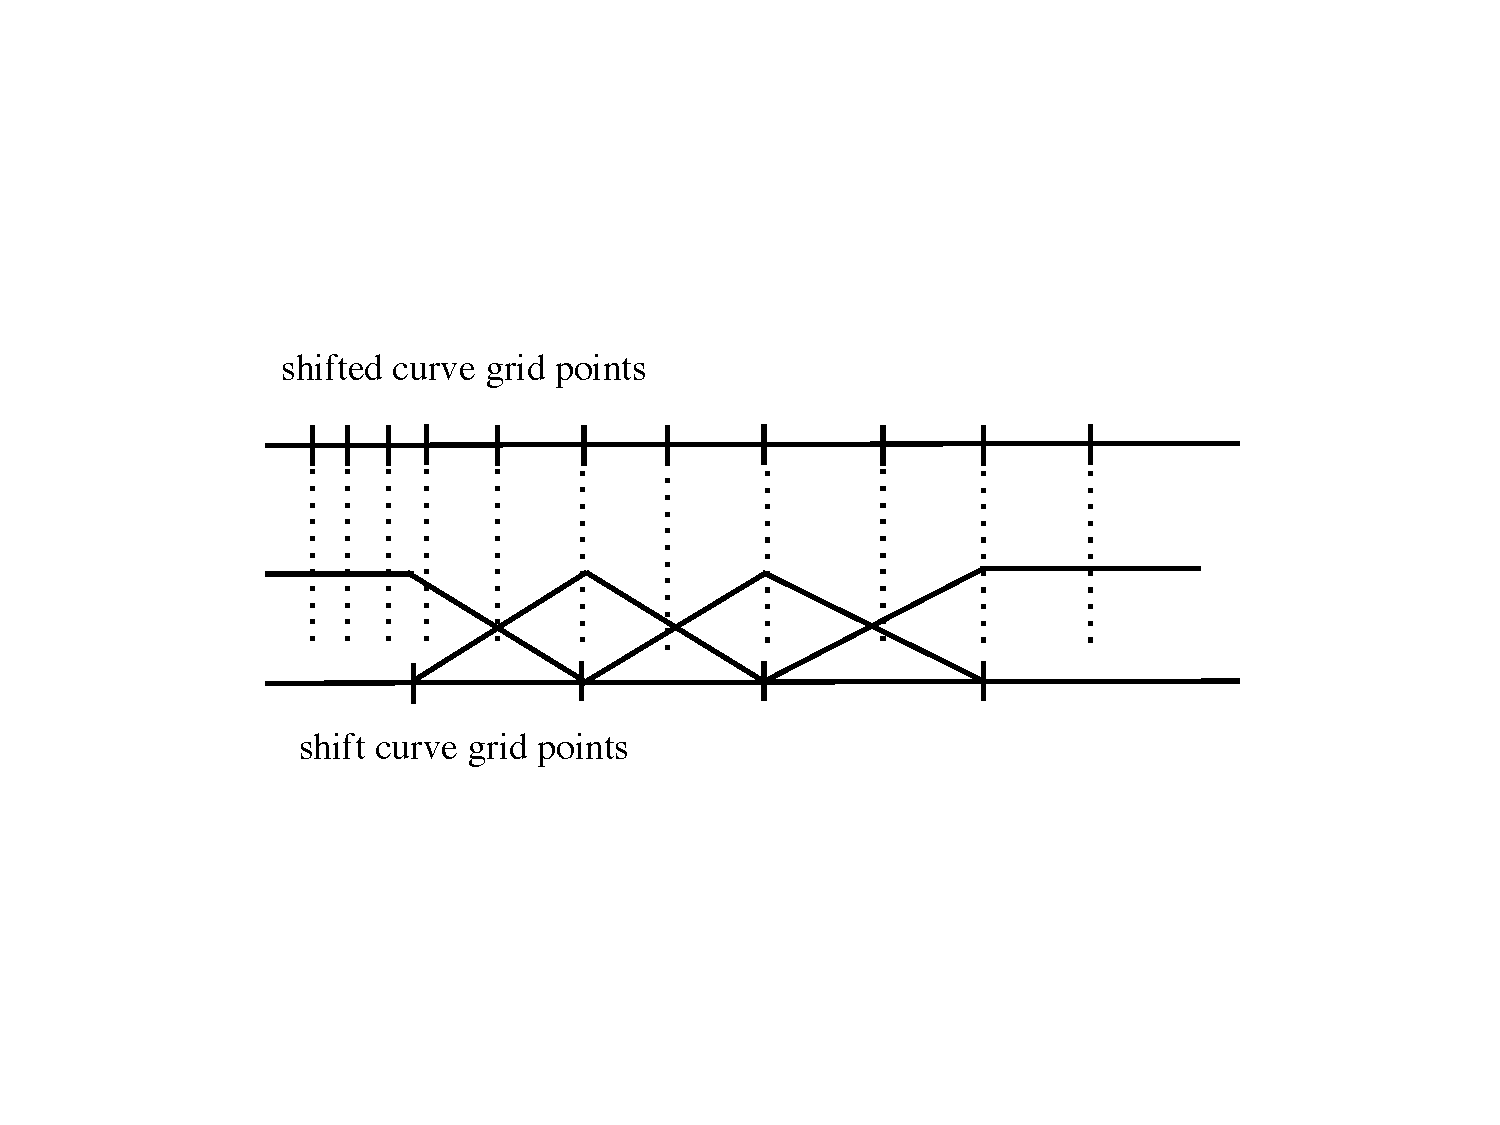
\includegraphics[scale=0.6]{shiftcurve.pdf}
\end{center}
\caption{1-d shift curve (bottom) applied to a more granular underlying curve (top). }
\label{fig_shiftcurve}
\end{figure} 

Shifts at the left and right end of the shift curve are extrapolated flat, i.e. applied to all data of the original curve to the left and to the right of the shift curve ends. In between, all shifts are distributed linearly as indicated to the left and right up to the adjacent shift grid points. As a result, a parallel shift of the all points on the shift curve yields a parallel shift of all points on the underlying curve.   \\

The two-dimensional case is covered in an analogous way, applying flat extrapolation at the boundaries and ``pyramidal-shaped'' linear interpolation for the bulk of the points. 

The details of the computation of sensitivities to implied volatilities in strike direction can be summarised as
follows, see also table \ref{sensi_config_overview} for an overview of the admissible configurations and the results
that are obtained using them.

\medskip
For {\em Swaption Volatilities}, the initial market setup can be an ATM surface only or a full cube. The simulation
market can be set up to simulate ATM only or to simulate the full cube, but the latter choice is only possible if a full cube is set
up in the initial market. The sensitivity set up must match the simulation setup with regards to the strikes (i.e. it
is ATM only if and only if the simulation setup is ATM only, or it must contain exactly the same strike spreads relative
to ATM as the simulation setup). Finally, if the initial market setup is a full cube, and the simulation / sensitivity
setup is to simulate ATM only, then sensitivities are computed by shifting the ATM volatility w.r.t. the given shift size and type and
shifting the non-ATM volatilities by the same absolute amount as the ATM volatility.

\medskip
For {\em Cap/Floor Volatilities}, the initial market setup always contains a set of fixed strikes, i.e. there is no
distinction between ATM only and a full surface. The same holds for the simulation market setup. The sensitivity setup
may contain a different strike grid in this case than the simulation market. Sensitivity are computed per expiry and
per strike in every case.

\medskip
For {\em Equity Volatilities}, the initial market setup can be an ATM curve or a full surface. The simulation market can
be set up to simulate ATM only or to simulate the full surface, where a full surface is allowed even if the initial market setup in an
ATM curve only. If we have a full surface in the initial market and simulate the ATM curve only in the simulation market, sensitivities
are computed as in the case of Swaption Volatilities, i.e. the ATM volatility is shifted w.r.t. the specified shift size
and type and the non-ATM volatilities are shifted by the same absolute amount as the ATM volatility. If the simulation
market is set up to simulate the full surface, then all volatilities are shifted individually using the specified shift size and type. In
every case the sensitivities are aggregated on the ATM bucket in the sensitivity report.

\medskip
For {\em FX Volatilities}, the treatment is similar to Equity Volatilities, except for the case of a full surface
definition in the initial market and an ATM only curve in the simulation market. In this case, the pricing in the
simulation market is using the ATM curve only, i.e. the initial market's smile structure is lost.

\medskip
For {\em CDS Volatilities} only an ATM curve can be defined.

\medskip
In all cases the smile dynamics is ``sticky strike'', i.e. the implied vol used for pricing a deal does not change if
the underlying spot price changes.

\begin{table}[hbt]
  \scriptsize
  \begin{center}
    \begin{tabular}{l | l | l | l | l | l}
      \hline
      Type & Init Mkt. Config. & Sim. Mkt Config. & Sensitivity Config. & Pricing & Sensitivities w.r.t. \\
      \hline
      Swaption & ATM & Simulate ATM only & Shift ATM only & ATM Curve & ATM Shifts \\
      Swaption & Cube & Simulate Cube & Shift Smile Strikes & Full Cube & Smile Strike Shifts\footnote{smile
                                                                          strike spreads must match simulation market configuration} \\
      Swaption & Cube & Simulate ATM only & Shift ATM only & Full Cube & ATM Shifts\footnote{smile is shifted in parallel\label{sensismileparallel}} \\
      \hline
      Cap/Floor & Surface & Simulate Surface & Shift Smile Strikes & Full Surface & Smile Strike Shifts \\
      \hline
      Equity & ATM & Simulate ATM only & Shift ATM only & ATM Curve & ATM Shifts \\
      Equity & ATM & Simulate Surface & Shift ATM only & ATM Curve & Smile Strike Shifts\footnote{result sensitivities
                                                                     are aggregated on ATM\label{sensiaggatm}} \\
      Equity & Surface & Simulate ATM only & Shift ATM only & Full Surface & ATM Shifts\textsuperscript{\ref{sensismileparallel}} \\
      Equity & Surface & Simulate Surface & Shift ATM only & Full Surface & Smile Strike Shifts\textsuperscript{\ref{sensiaggatm}} \\
      \hline
      FX & ATM & Simulate ATM only & Shift ATM only & ATM Curve & ATM Shifts \\
      FX & ATM & Simulate Surface & Shift ATM only & ATM Curve & Smile Strike Shifts\textsuperscript{\ref{sensiaggatm}} \\
      FX & Surface & Simulate ATM only & Shift ATM only & ATM Curve & ATM Shifts \\
      FX & Surface & Simulate Surface & Shift ATM only & Full Surface & Smile Strike Shifts\textsuperscript{\ref{sensiaggatm}} \\
      \hline
      CDS & ATM & Simulate ATM only & Shift ATM only & ATM Curve & ATM Shifts \\
    \end{tabular}
    \caption{Admissible configurations for Sensitivity computation in ORE}
    \label{sensi_config_overview}
  \end{center}
  \end{table}

\subsection{Par Sensitivity Analysis}
\label{app:par_sensi}

The ``raw'' sensitivities in ORE are generated in a computationally convenient domain (such as zero rates, caplet/floorlet volatilities, integrated hazard rates, inflation zero rates). These raw sensitivities are typically further processed in risk analytics such as VaR measures. On the other hand, for hedging purposes one is rather interested in sensitivities with respect to fair rates of hedge instruments such as Forward Rate Agreements, Swaps, flat Caps/Floors, CDS, Zero Coupon Inflation Swaps. \\

It is possible to generate par sensitivities from raw sensitivities using the chain rule as follows, and this is the approach taken in ORE. Recall for example the fair swap rate $c$ for some maturity as a function of zero rates $z_i$ in a single curve setting:
$$
c = \frac{1 - e^{-z_n\,t_n}}{\sum_{i=1}^n \delta_i\,e^{-z_i\, t_i}}
$$
More realistically, a given fair swap rate might be a function of the zero rates spanning the discount and index curves in the chosen currency. In a multi currency curve setting, that swap rate might even be a function of the zero rates spanning a foreign (collateral) currency discount curve, foreign and domestic currency index curves. Generally, we can write any fair par rate $c_i$ as function of raw rates $z_j$,
$$
c_i \equiv c_i(z_1, z_2, ..., z_n)
$$
This function may not be available in closed form, but numerically we can evaluate the sensitivity of $c_i$ with respect to changes in all raw rates,
$$
\frac{\partial c_i}{\partial z_j}.
$$
These sensitivities form a {\em Jacobi} matrix of derivatives. Now let $V$ denote some trade's price. Its sensitivity with respect a raw rate change $\partial V/\partial z_k$ can then be expressed in terms of sensitivities w.r.t. par rates using the chain rule
$$
\frac{\partial V}{\partial z_j} = \sum_{i=1}^n \frac{\partial V}{\partial c_i}\,\frac{\partial c_i}{\partial z_j},
$$
or in vector/matrix form
$$
\nabla_z V = C \cdot \nabla_c V, \qquad C_{ji} = \frac{\partial c_i}{\partial z_j}.
$$
Given the raw sensitivity vector $\nabla_z V$, we need to invert the Jacobi matrix $C$ to obtain the par rate sensitivity vector
$$
\nabla_c V = C^{-1} \cdot \nabla_z V.
$$

We then compute the Jacobi matrix $C$ by
\begin{itemize}
\item setting up par instruments with links to all required term structures expressed in terms of raw rates
\item ``bumping'' all relevant raw rates and numerically computing the par instrument's fair rate shift for each bump
\item thus filling the Jacobi matrix with finite difference approximations of the partial derivatives $\partial c_i/\partial z_j$.
\end{itemize}

The par rate conversion supports the following par instruments:
\begin{itemize}
\item Deposits
\item Forward rate Agreements
\item Interest Rate Swaps (fixed vs. ibor)
\item Overnight Index Swaps
\item Tenor Basis Swaps (ibor vs. ibor)
\item Overnight Index Basis Swaps (ibor vs. OIS)
\item FX Forwards
\item Cross Currency Basis Swaps
\item Credit Default Swaps
\item Caps/Floors
\end{itemize}


\subsection{Value at Risk}\label{sec:app_var}

For the computation of the parametric, or variance-covariance VaR, we rely on a second order sensitivity-based P\&L approximation

\begin{eqnarray}\label{taylorPl2}
  \pi_S & = & \sum_{i=1}^n D^i_{T_i}\,V\cdot Y_i 
        + \frac{1}{2} \sum_{i,j=1}^n D^{i,j}_{T_i,T_j}\,V\cdot Y_i\cdot Y_j
\end{eqnarray}

with 
\begin{itemize}
\item portfolio value $V$
\item random variables $Y_i$ representing risk factor returns; these are assumed to be multivariate normally distributed with zero mean
and covariance matrix matrix $C = \{ \rho_{i,k} \sigma_i \sigma_k \}_{i,k}$, where $\sigma_i$ denotes the standard
deviation of $Y_i$; covariance matrix $C$ may be estimated using the Pearson estimator on historical return data
$\{ r_i(j) \}_{i,j}$. Since the raw estimate might not be positive semidefinite, we apply a salvaging algorithm to
ensure this property, which basically replaces negative Eigenvalues by zero and renormalises the resulting matrix, see
\cite{corrSalv};
\item first or second order derivative operators $D$, depending
on the market factor specific shift type $T_i \in \{ A,R,L \}$ (absolute shifts, relative shifts, absolute log-shifts), i.e.
\begin{eqnarray*}\label{derivs}
  D^i_A \,V(x) &=& \frac{\partial V(x)}{\partial x_i} \\
  D^i_R \,V(x) = D^i_L f(x) &=& x_i\frac{\partial V(x)}{\partial x_i}
\end{eqnarray*}
and using the short hand notation
\begin{equation*}
  D^{i,j}_{T_i,T_j} V(x) = D^i_{T_i} D^j_{T_j} V(x)
\end{equation*}
In ORE, these first and second order sensitivities are computed as finite difference
approximations (``bump and revalue'').
\end{itemize}

To approximate the $p$-quantile of $\pi_S$ in \eqref{taylorPl2} ORE offers the techniques outlined below.

\subsubsection*{Delta Gamma Normal Approximation}
 
The distribution of \eqref{taylorPl2} is non-normal due to the second order terms. 
The delta gamma normal approximation in ORE computes mean $m$ and variance $v$ of the portfolio value change $\pi_S$ (discarding moments higher than two) following \cite{alexander} and provides a simple VaR estimate 
$$
VaR = m + N^{-1}(q)\,\sqrt{v}
$$
for the desired quantile $q$ ($N$ is the cumulative standard normal distribution). Omitting the second order terms in \eqref{taylorPl2} yields the delta normal approximation.
 
\subsubsection*{Cornish-Fisher Expansion}

The first four moments of the distribution of $\pi_S$ in \eqref{taylorPl2} can be computed in closed form using the covariance matrix $C$ and the sensitivities of first and second order $D_i$
and $D_{i,k}$, see e.g. \cite{alexander}. Once these moments are known, an approximation to the true quantile of $\pi_S$ can be computed using the Cornish-Fisher expansion, see also [7], which in practice often gives a decent approximation of the true value, but may also show bigger differences in certain configurations.

\subsubsection*{Saddlepoint Approximation}

Another approximation of the true quantile of $\pi_S$ can be computed using the Saddlepoint approximation using results from \cite{Lugannani} and \cite{Daniels}. This method typically produces more accurate results than the Cornish-Fisher method, while still being fast to evaluate.

\subsubsection*{Monte Carlo Simulation}

By simulating a large number of realisations of the return vector $Y=\{ Y_i \}_i$ and computing the corresponding
realisations of $\pi_S$ in \eqref{taylorPl2} we can estimate the desired quantile as the quantile of the empirical
distribution generated by the Monte Carlo samples. Apart from the Monte Carlo Error no approximation is involved in this
method, so that albeit slow it is well suited to produce values against which any other approximate approaches can be tested. Numerically, the simulation is implemented using a Cholesky Decomposition
of the covariance matrix $C$ in conjunction with a pseudo random number generator (Mersenne Twister) and an
implementation of the inverse cumulative normal distribution to transform $U[0,1]$ variates to $N(0,1)$ variates.

\end{appendix}

%========================================================
%\section{References}
%========================================================

\begin{thebibliography}{*}

\bibitem{ORE} \url{http://www.opensourcerisk.org}

\bibitem{QL} \url{http://www.quantlib.org}
 
\bibitem{QRM} \url{http://www.quaternion.com}

\bibitem{acadia} \url{http://www.acadia.inc}

\bibitem{quantlib-install} \url{http://quantlib.org/install/vc10.shtml}

%\bibitem{confluence} https://confluence.atlassian.com/bitbucket/set-up-git-744723531.html

\bibitem{git-download} \url{https://git-scm.com/downloads}

\bibitem{boost-binaries} \url{https://sourceforge.net/projects/boost/files/boost-binaries}

\bibitem{boost} \url{http://www.boost.org}

\bibitem{jupyter} \url{http://jupyter.org}

\bibitem{Anaconda} \url{https://docs.continuum.io/anaconda}

\bibitem{LO} \url{http://www.libreoffice.org}

%\bibitem{xlwings} \url{http://www.xlwings.org}

\bibitem{bcbs128} Basel Committee on Banking Supervision, {\em International Convergence of Capital Measurement and
    Capital Standards, A Revised Framework}, \url{http://www.bis.org/publ/bcbs128.pdf}, June 2006

\bibitem{bcbs189} Basel Committee on Banking Supervision, {\em Basel III: A global regulatory framework for more
    resilient banks and banking systems}, \url{http://www.bis.org/publ/bcbs189.pdf}, June 2011

\bibitem{d325} Basel Committee on Banking Supervision, {\em Review of the Credit Valuation Adjustment Risk Framework}, \url{https://www.bis.org/bcbs/publ/d325.pdf}, 2015

\bibitem{d424} Basel Committee on Banking Supervision, {\em Basel III: Finalising post-crisis reforms}, \url{https://www.bis.org/bcbs/publ/d424.pdf}, 2017

\bibitem{BrigoMercurio} Damiano Brigo and Fabio Mercurio, {\em Interest Rate Models: Theory and Practice, 2nd Edition},
  Springer, 2006.

\bibitem{Pykhtin2010} Michael Pykhtin, {\em Collateralized Credit Exposure}, in Counterparty Credit Risk, (E. Canabarro,
  ed.), Risk Books, 2010

\bibitem{PykhtinRosen} Michael Pykhtin and Dan Rosen, {\em Pricing Counterparty Risk at the Trade Level and CVA
    Allocations}, Finance and Economics Discussion Series, Divisions of Research \& Statistics and Monetary Affairs,
  Federal Reserve Board, Washington, D.C., 2010

\bibitem{Gregory12} Jon Gregory, {\em Counterparty Credit Risk and Credit Value Adjustment, 2nd Ed.}, Wiley Finance,
  2013.

\bibitem{Gregory15} Jon Gregory, {\em The xVA Challenge, 3rd Ed.}, Wiley Finance, 2015.

\bibitem{Lichters} Roland Lichters, Roland Stamm, Donal Gallagher, {\em Modern Derivatives Pricing and Credit Exposure
    Analysis, Theory and Practice of CSA and XVA Pricing, Exposure Simulation and Backtesting}, Palgrave Macmillan,
  2015.

\bibitem{Anfuso2016} Fabrizio Anfuso, Daniel Aziz, Paul Giltinan, Klearchos Loukopoulos, {\em A Sound Modelling and
    Backtesting Framework for Forecasting Initial Margin Requirements},
  \url{http://papers.ssrn.com/sol3/papers.cfm?abstract_id=2716279}, 2016

\bibitem{Andersen2016} Leif B. G. Andersen, Michael Pykhtin, Alexander Sokol, {\em Rethinking Margin Period of Risk},
  http://papers.ssrn.com/sol3/papers.cfm?abstract\_id=2719964, 2016

  % \bibitem{SIMM}{SIMM Methodology\\ \tiny
  %   http://www2.isda.org/attachment/ODM1Mw==/ISDA\%20SIMM\%20Methodology\_7\%20April\%202016\_v3.15\%20(PUBLIC).pdf}

  % \bibitem{SIMM_Data_Standards}{SIMM Risk Data Standards\\ \tiny
  %   https://www2.isda.org/attachment/ODQzMg==/Risk\%20Data\%20Standards\_24\%20May\%202016\_v1.22\%20(PUBLIC).pdf}

  % \bibitem{OO} http://www.openoffice.org

\bibitem{Andersen_Piterbarg_2010} Andersen, L., and Piterbarg, V. (2010): Interest Rate Modeling, Volume I-III
  
\bibitem{LichtersEtAl} Peter Caspers, Paul Giltinan, Paul; Lichters, Roland; Nowaczyk , Nikolai. {\em Forecasting Initial Margin Requirements – A Model Evaluation}, Journal of Risk Management in Financial Institutions, Vol. 10 (2017), No. 4, \url{https://ssrn.com/abstract=2911167}

\bibitem{corrSalv} R. Rebonato and P. Jaeckel, The most general methodology to create a valid correlation matrix for
  risk management and option pricing purposes, The Journal of Risk, 2(2), Winter 1999/2000,
  \url{http://www.quarchome.org/correlationmatrix.pdf}

\bibitem{alexander} Carol Alexander, Market Risk Analysis, Volume IV, Value at Risk Models, Wiley 2009

\bibitem{Lugannani} Lugannani, R.and S.Rice (1980), Saddlepoint Approximations for the Distribution of the Sum of
  Independent Random Variables, Advances in Applied Probability, 12,475-490.

\bibitem{Daniels} Daniels, H. E. (1987), Tail Probability Approximations, International Statistical Review, 55, 37-48.

\end{thebibliography}

\newpage
\addcontentsline{toc}{section}{Todo}
\listoftodos[Todo]
%\todos

\end{document}
